\documentclass{book}
\usepackage{physics}
\usepackage{graphicx}
\usepackage{caption}
\usepackage{amsmath}
\usepackage{bm}
\usepackage{authblk}
\usepackage{empheq}
\usepackage{amsfonts}
\usepackage{esint}
\usepackage[makeroom]{cancel}
\usepackage{dsfont}
\usepackage{centernot}
\usepackage{mathtools}
\usepackage{bigints}
\usepackage{amsthm}
\theoremstyle{definition}
\newtheorem{defn}{Definition}[section]
\newtheorem{prop}{Proposition}[section]
\newtheorem{rmk}{Remark}[section]
\newtheorem{thm}{Theorem}[section]
\newtheorem{exmp}{Example}[section]
\newtheorem{prob}{Problem}[section]
\newtheorem{sln}{Solution}[section]
\newtheorem*{prob*}{Problem}
\newtheorem{exer}{Exercise}[section]
\newtheorem*{exer*}{Exercise}
\newtheorem*{sln*}{Solution}
\usepackage{empheq}
\usepackage{hyperref}
\usepackage{tensor}
\usepackage{xcolor}
\hypersetup{
	colorlinks,
	linkcolor={black!50!black},
	citecolor={blue!50!black},
	urlcolor={blue!80!black}
}


\newcommand*\widefbox[1]{\fbox{\hspace{2em}#1\hspace{2em}}}

\newcommand{\p}{\partial}
\newcommand{\R}{\mathbb{R}}
\newcommand{\C}{\mathbb{C}}
\newcommand{\lag}{\mathcal{L}}
\newcommand{\nn}{\nonumber}
\newcommand{\ham}{\mathcal{H}}
\newcommand{\M}{\mathcal{M}}
\newcommand{\I}{\mathcal{I}}
\newcommand{\K}{\mathcal{K}}
\newcommand{\F}{\mathcal{F}}
\newcommand{\w}{\omega}
\newcommand{\lam}{\lambda}
\newcommand{\al}{\alpha}
\newcommand{\be}{\beta}
\newcommand{\x}{\xi}

\newcommand{\G}{\mathcal{G}}

\newcommand{\f}[2]{\frac{#1}{#2}}

\newcommand{\ift}{\infty}

\newcommand{\lp}{\left(}
\newcommand{\rp}{\right)}

\newcommand{\lb}{\left[}
\newcommand{\rb}{\right]}

\newcommand{\lc}{\left\{}
\newcommand{\rc}{\right\}}


\newcommand{\V}{\mathbf{V}}
\newcommand{\U}{\mathcal{U}}
\newcommand{\Id}{\mathcal{I}}
\newcommand{\D}{\mathcal{D}}
\newcommand{\Z}{\mathcal{Z}}

%\setcounter{chapter}{-1}


\makeatletter
\renewcommand{\@chapapp}{Part}
%\renewcommand\thechapter{$\bf{\ket{\arabic{chapter}}}$}
%\renewcommand\thesection{$\bf{\ket{\arabic{section}}}$}
%\renewcommand\thesubsection{$\bf{\ket{\arabic{subsection}}}$}
%\renewcommand\thesubsubsection{$\bf{\ket{\arabic{subsubsection}}}$}
\makeatother



\usepackage{subfig}
\usepackage{listings}
\captionsetup[lstlisting]{margin=0cm,format=hang,font=small,format=plain,labelfont={bf,up},textfont={it}}
\renewcommand*{\lstlistingname}{Code \textcolor{violet}{\textsl{Mathematica}}}
\definecolor{gris245}{RGB}{245,245,245}
\definecolor{olive}{RGB}{50,140,50}
\definecolor{brun}{RGB}{175,100,80}
\lstset{
	tabsize=4,
	frame=single,
	language=mathematica,
	basicstyle=\scriptsize\ttfamily,
	keywordstyle=\color{black},
	backgroundcolor=\color{gris245},
	commentstyle=\color{gray},
	showstringspaces=false,
	emph={
		r1,
		r2,
		epsilon,epsilon_,
		Newton,Newton_
	},emphstyle={\color{olive}},
	emph={[2]
		L,
		CouleurCourbe,
		PotentielEffectif,
		IdCourbe,
		Courbe
	},emphstyle={[2]\color{blue}},
	emph={[3]r,r_,n,n_},emphstyle={[3]\color{magenta}}
}

\begin{document}
\begin{titlepage}\centering
 \clearpage
 \title{\textsc{\bf{CLASSICAL FIELD THEORY}}\\\smallskip - A Quick Guide -\\}
 \author{\bigskip Huan Q. Bui}
 \affil{Colby College\\$\,$\\ PHYSICS \& MATHEMATICS\\ Statistics \\$\,$\\Class of 2021\\}
 \date{\today}
 \maketitle
 \thispagestyle{empty}
\end{titlepage}

\newpage

\subsection*{Preface}
\addcontentsline{toc}{subsection}{Preface}

Greetings,\\

\textit{Classical Field Theory, A Quick Guide to} is compiled based on my independent study PH491/2: Topics in Classical Field Theory notes with professor Robert Bluhm. Sean Carroll's \textit{Spacetime and Geometry: An Introduction to General Relativity}, along with other resources, serves as the main guiding text. This text also references a number of other texts such as \textit{Quantum Field Theory} by Ryder, \textit{Quantum Field Theory} by Mandl and Shaw, \textit{Gauge Theories Of The Strong, Weak, and Electromagnetic Interactions} by Quigg, \textit{A First Book of Quantum Field Theory} by A. Lahiri and P. B. Pal, \textit{Quantum Field Theory in a Nutshell} by Zee.   \\

This text is a continuation of \textit{General Relativity and Cosmology, A Quick Guide to}. Familiarity with classical mechanics, linear algebra, vector calculus, and especially general relativity is expected. There will be a quick review of general relativity where important concepts are revisited and derivations highlighted, but familiarity with basic notions such as geodesics, Christoffel symbols, the Riemann curvature tensors, etc. is assumed. \\ 

Note: As a consequence of being developed from a variety of sources, there will be some overlapping among the sections. However, the objective of each section is unique.\\

Enjoy!


\newpage

\tableofcontents

\newpage
\chapter{Introduction to the Lagrangian and the Principle of Least Action}
\begin{prop}
	All fundamental physics obeys least action principles.
\end{prop}
The action $S$ is defined as
\begin{align}
S = \int_{a}^{b}\mathcal{L}\,dt.
\end{align}
where $\mathcal{L}$ is called the Lagrangian.\\

Refer for Farlow's \textit{Partial Differential Equation}, page 353, for detailed explanation of Lagrange's calculus of variations.\\

I will derive the Euler-Lagrange equation(s) here, but we are not going to use it in the following subsection for the introduction to field theory for now. \\
\begin{align}
\frac{\partial \mathcal{L}}{\partial \phi} - \partial_\mu\frac{\partial \mathcal{L}}{\partial(\partial_\mu \phi)} = 0.
\end{align}
\section{A Classical-Mechanical Example}
In this subsection we take a look at how the Lagrangian formulation of classical mechanics can give rise to Newton's second law of motion. In mechanics, the Lagrangian often takes the form:
\begin{align}
\mathcal{L} = K - V,
\end{align}
where $K$ is the kinetic energy, and $V$ is the potential energy. Let us consider a simple example where
\begin{align}
K &= \frac{1}{2}m\dot{x}^2\\
V &= V(x).
\end{align}
Variations on the Lagrangian gives
\begin{align}
\delta \mathcal{L} &= \delta\left( \frac{1}{2}m\dot{x}^2 - V(x) \right)\\
&= m\dot{x}\delta \dot{x} - \frac{dV}{dx}\delta x\\
&= m\dot{x}\dot{\delta x} - \frac{dV}{dx}\delta x\\
&= m \left( -\ddot{x}\delta x + \frac{d}{dt}\dot{x}\delta x \right) - \frac{dV}{dx}\delta x\\
&= -m\ddot{x}\delta x - m\frac{d}{dt}\dot{x}\delta x - \frac{dV}{dx}\delta x. 
\end{align}
It follows that the variations on the action gives
\begin{align}
\delta S = \int_{a}^{b}\delta L \,dt = -\int_a^b\left( m\ddot{x} + \frac{dV}{dx} \right)\delta x\,dt.
\end{align}
The principle of least action requires $\delta S = 0$ for all $\delta x$. Therefore it follows that
\begin{align}
m\ddot{x} + \frac{dV}{dx} = 0,
\end{align}
which is simply Newton's second law of motion in disguise. \\

Before we move on, we should note that in order for the Lagrangian formulation to work in electromagnetism or in general relativity, we need to promote the Lagrangian to its relativistic version where the Lagrangian is given by
\begin{align}
L = \int_a^b\mathcal{L}\,d^3x.
\end{align}
$\mathcal{L}$ is called the Lagrangian density, but we can colloquially refer to it as ``the Lagrangian.'' The relativistic action hence takes the form
\begin{align}
S = \int \mathcal{L}\,d^4x,
\end{align}
where $d^4x$ implies integrating over all spacetime.

\newpage
\chapter{Group Theory: a quick guide in a quick guide}
\begin{enumerate}
	\item Consider an N-dimensional vector with complex elements. A gauge transformation that takes $\vert z\vert^2 \to \vert z \vert^2$ (modulus preserving) is call a U(N) gauge transformation. The letter ``U'' denotes ``unitary.'' These kinds of transformations can be represented by a unitary matrix, which is defined as a matrix whose conjugate transpose is the same as its inverse. If $z\to Uz$, then 
	\begin{align}
	\vert z\vert^2 \to (Uz)^\dagger(Uz) = z^\dagger U^\dagger U z =z^\dagger z =\vert z\vert^2,
	\end{align} 
	hence modulus preserving.\\
	
	Note that the transformation $e^{i\alpha}$ is unitary. It is simply a 1$\times$1 unitary matrix. This immediately implies that complex scalars have a U(1) gauge invariance.\\
	
	The special group of U(N) transformations is denoted SU(N), which represents those with $\det U= 1$. 
	\item Consider another N-dimensional real-valued-element vector. We denote the group of orthogonal transformations O(N). Orthogonal transformations are orthogonal, i.e., length-preserving. 
	\begin{align}
	(Ox)^\top(Ox) = x^\top O^\top O x = x^\top x = \vec{x}^2
	\end{align} 
	Once again, we denote the special group of the O(N) the SO(N) group. This group represents transformations with $\det O = 1$. The Lorentz group is a sub-group of SO(N), as the norm is defined differently, nevertheless it is still length-preserving. We call the Lorentz group SO(3,1), signifying that one sign is different from the other three. 
\end{enumerate}



\newpage

\chapter{Introduction to Classical Field Theory}
\section{Relativistic Notation}
Throughout this text, we will use the particle physics' Minkowski spacetime metric tensor:
\begin{align}
\eta_{\mu\nu} = \begin{pmatrix}
1&0&0&0\\
0&-1&0&0\\
0&0&-1&0\\
0&0&0&-1
\end{pmatrix}.
\end{align}
We shall assume knowledge of inner products and index-lowering/raising operations (please refer to \textit{General Relativity \& Cosmology: A Quick Guide to}) for more details about this ``indexing'' business. \\

Quick notes: the four-dimensional generalization of the gradient operator $\nabla$ transforms like a four-vector. If $\phi(x)$ is a scalar function, so is
\begin{align}
\delta \phi = \frac{\p \phi}{\p x^\mu}\delta x^\mu
\end{align}
and so
\begin{align}
\frac{\p \phi}{\p x^\mu} \equiv \p_\mu \phi \equiv \phi,_\mu.
\end{align}
Similarly, we also have something for the contravariant four-vector:
\begin{align}
\frac{\p \phi}{\p x_\mu} \equiv \p^\mu \phi \equiv \phi,^\mu.
\end{align}
Lastly, we define the \textbf{d'Alembertian} as:
\begin{align}
\square \equiv \frac{\p^2}{\p t^2} - \p^\mu \p_\mu.
\end{align}
These will come in handy when we ``vary'' the action and the Lagrangian - but more on this later. 

\section{Classical Lagrangian Field Theory}
In classical field theory, we are interested in fields, or systems of fields. We can consider a system which requires several fields, $\phi_r(x)$, where $r=1,\dots,N$. We are also interested in the Lagrangian density, which has a more general form than we have seen in the first section when we are still in the realm of Newtonian physics:
\begin{align}
\lag = \lag(\phi_r, \phi_{r,a}),
\end{align}
where we have used the covariant notation to denote derivatives of $\phi$ with respect to the coordinates. The action, as integrated over some region $\Omega$ of four-spacetime, is then given by
\begin{align}
S(\Omega) = \int_\Omega \lag(\phi, \phi_{r,a})\,d^4x.
\end{align}
Now, consider a variation in the field
\begin{align}
\phi_r(x) \to \phi_r(x) + \delta \phi_r(x)
\end{align}
with the requirement that
\begin{align}
\delta \phi_r(x) 0
\end{align}
 on the boundary of $\Omega$. As we will explore later on, the field $\phi$ can be real or complex. In the case of the complex field, we can simply treat $\phi$ and its complex conjugate $\phi^*$ as two independent fields. However, whether $\phi$ is complex or not should not matter in what we are doing now, which is requiring that the variation in the action to take a stationary value, i.e.,
 \begin{align}
 \delta S = 0.
 \end{align}
So,
\begin{align}
0 = \delta S &= \int_\Omega  d^4x\,\left\{ \frac{\p\lag}{\p\phi_r}\delta \phi_r + \frac{\p\lag}{\p\phi_{r,a}}\delta \phi_{r,a}    \right\}\\
&= \int_\Omega d^4x\, \left\{ \frac{\p\lag}{\p\phi_r} - \frac{\p}{\p x^a}\left( \frac{\p\lag}{\p\phi_{r,a}} \right) \right\}\delta \phi_r +  \int_\Omega d^4x\,\frac{\p}{\p x^a}\left(\frac{\p\lag}{\p\phi_{r,a}}\p \phi_r \right)
\end{align}
where the second line simply comes from doing integration by parts and the covariant notation:
\begin{align}
\delta \phi_{r,a} = \frac{\p}{\p x^a}\delta \phi_r.
\end{align}
Now, the second term on the second line can be re-written under Gauss-Ostrogradsky's theorem as
\begin{align}
\int_\Omega d^4x\,\frac{\p}{\p x^a}\left(\frac{\p\lag}{\p\phi_{r,a}}\p \phi_r \right) = 
\int_{\delta \Omega}d^3x\,  \frac{\p\lag}{\p\phi_{r,a}}\p \phi_r
\end{align}
where the $\p_a$ denotes a divergence and $\delta \Omega$ denotes the boundary of the region in spacetime. But notice that since we require the variation to vanish at the boundary of $\Omega$, this integral simply vanishes, so the variation in the action becomes
\begin{align}
0 = \delta S = \int_\Omega d^4x\, \left\{ \frac{\p\lag}{\p\phi_r} - \frac{\p}{\p x^a}\left( \frac{\p\lag}{\p\phi_{r,a}} \right) \right\}\delta \phi_r.
\end{align}
Now, because this equality has to hold for any variation $\delta \phi_r$, it must be true that the integrand has to be zero. We arrive at the Euler-Lagrange equation:
\begin{align}
\frac{\p\lag}{\p\phi_r} - \frac{\p}{\p x^a}\left( \frac{\p\lag}{\p\phi_{r,a}} \right) = 0.
\end{align}

\section{Quantized Lagrangian Field Theory (primer)}
While the focus of this text is classical field theory, it can be worthwhile to have a little primer on what quantized Lagrangian field theory looks like. The main difference between classical and quantized Lagrangian field theory is the ``degree of freedom'' in the field. In classical field theory, we deal with systems with a continuously infinite number of degrees of freedom, i.e. at any point in spacetime, the field $\phi$ is assigned some value. In quantized field theory, we consider an ``approximation'' of this by imagining a system with a countable number of degrees of freedom, and then go to the continuum limit.\\

Consider flat spacetime, at an instance $t = Constant$. Let us now make space discrete by thinking of space as ``cells'' of equal volume called $\delta x_i$ where $i$ is just another index. Let the value of the field within each cell by the value of the field at the center of the cell. So now the system is discrete and can be described by a discrete set of generalized coordinates:
\begin{align}
q_{ri}(t) \equiv \phi_r(\mathbf{x}_i, t)
\end{align} 
where $q_{ri}(t)$ simply represents the value of the field $\phi_r$ at cell $\mathbf{x}_i$ at time $t$. Now, since the idea of the derivative no longer holds in the discrete world, the new Lagrangian density takes into account the difference in the field values between neighboring cells. This gives the \textit{Lagrangian}, $L$, NOT the \textit{Lagrangian density} (the Lagrangian density is denoted $\lag$):
\begin{align}
L(t) = \sum_{i} \delta \mathbf{x}_i \lag_i (\phi_r(i,t), \dot{\phi}_r(i,t), \phi_r(i',t))
\end{align} 
Now, recall from classical mechanics that the second term in the Euler-Lagrange equation represents the momentum, so we define the \textbf{momentum conjugate} to $q_{ri}$ as
\begin{align}
p_{ri} &= \frac{\p L}{\p \dot{q}_{ri}}\\
&= \frac{\p L}{\p \dot{\phi}_r(i,t)}\\
&= \frac{\p}{\p \dot{\phi}_r(i,t)}\sum_{i} \delta \mathbf{x}_i \lag_i \\
&= \pi_r(i,t)\delta \mathbf{x}_i
\end{align}
where 
\begin{align}
\pi_r(i,t) = \frac{\p\lag_i}{\p \dot{q}_r(i,t)} =\frac{\p\lag_i}{\p \dot{\phi}_r(i,t)}
\end{align}
is called the \textbf{canonical momenta}. This definition makes sense by analogy to classical mechanics, as $q_{ri}$ is just the coordinates. So, the Hamiltonian of the discrete system is given by
\begin{align}
H &= \sum_{i}p_{i}\dot{q}_{ri} - L\\
&= \sum_{i}\delta\mathbf{x}_i \left\{\pi_r(i,t)\dot{\phi}_r(i,t) - \lag_i \right\}.
\end{align}
Now, letting the difference go to zero, i.e, $\delta \mathbf{x}_i \to 0$, which makes
\begin{align}
\pi_r(x) = \frac{\p\lag_i}{\p \dot{\phi}_r(i,t)} \to \frac{\p\lag_i}{\p \dot{\phi}_r},
\end{align}
i.e., 
\begin{align}
\pi_r(i,t) \to \pi_r(\mathbf{x}_i,t),
\end{align}
in which case the Lagrangian turns from a sum into an integral
\begin{align}
L(t) = \int d^3x\, \lag(\phi_r, \phi_{r,a})
\end{align}
and so does the Hamiltonian
\begin{align}
H = \int d^3x\, \mathcal{H}(x),
\end{align}
where the Hamiltonian density is given by (again, turned from a sum into an integral)
\begin{align}
\mathcal{H}(x) = \pi_r(x)\dot{\phi_r}(x) - \lag(\phi_r, \phi_{r,a}).
\end{align}
\section{Symmetries and Conservation Laws (primer)}
Recall the Heisenberg's equation of motion of an operator $O(t)$:
\begin{align}
i\hbar \frac{dO(t)}{dt} = [O(t), H],
\end{align}
where $[.,.]$ denotes the commutator. Note that
\begin{align}
[O, H] = 0
\end{align}
if $O$ is a constant of motion, which often stem from invariance properties of systems under groups of transformation such as translation or rotations. These invariances relate to conservation laws, which we will explore in much more detail in the next sections. Consider an example with a wavefunction $\Psi$ and an operator $O$ undergoing a Lorentz transformation:
\begin{align}
\ket{\Psi} &\to \ket{\Psi'} = U\ket{\Psi}\\
O &\to O' = UOU^\dagger.
\end{align}
$U$ is a unitary transformation, which ensure that (i) the operator equations are covariant, and (ii) probability amplitudes and eigenvalues of operators (observables) are invariant (unitary matrices are length-preserving).\\

We can consider another example of a rotation in the complex plane:
\begin{align}
U = e^{i\alpha T}
\end{align}
where $U$ can be thought of as a unitary, continuous, 1$\times$1 transformation, and $T = T^\dagger$. For an infinitesimal transformation
\begin{align}
U \approx 1 + i\delta \alpha T
\end{align}
and hence
\begin{align}
O' = O \delta O = UOU^\dagger = (1+i\delta \alpha T)O(1-i\delta \alpha T),
\end{align}
which we can show to be equivalent to
\begin{align}
\delta O = i\delta \alpha[T,O].
\end{align}
So, if the operator $O$ is the Hamiltonian $H$, and by requiring the theory to be invariant under variations, i.e., $\delta H = 0$, which means
\begin{align}
[T,H] = 0,
\end{align}
which implies that $T$ is a constant of motion. \\

For a field theory derived from a Lagrangian density, we can construct conserved quantities from the invariance of $\lag$ under symmetry transformations. We have a prescription to do this where very first step is to show that we can construct a function $f^a$ of the field operators and derivatives such that
\begin{align}
\frac{\p f^a}{\p x^a} = 0.
\end{align}
where $a$ are just indices, and $x^0 \equiv t$. We will show how this is possible by first assuming that, well, it is possible - in which case if we define 
\begin{align}
F^a(t) = \int d^3x\, f^a(\mathbf{x},t) = Constant.
\end{align}
(this equation really hints to us that something is conserved over time... hence a requirement to construct conserved quantities) then by $\p f^a/\p x^a = 0$ we have
\begin{align}
\frac{dF^0}{dt} &= \frac{d}{dt} \int d^3x\, f^0(\mathbf{x},t)\\
&= \frac{d}{dt}Constant - \frac{d}{dt} \p_j f^j(\mathbf{x},t),\,\,\,\,\,\, j = 1,2,3\\
&= -\int d^3x\, \p_j f^j(\mathbf{x},t)\\
&= 0.
\end{align}
This means
\begin{align}
F^0 = \int d^3x\, f^0(\mathbf{x},t) = Constant,
\end{align}
i.e, $F^0$ is a conserved quantity we are talking about. But what exactly are the quantities $f$ and $F$ and how can we interpret them? As we go along, it will make more sense to call $f^a$ the \textit{conserved current}. We will also explore Noether's theorem that relates transformation symmetries and conservations later in the following sections.\\

Let us apply this result to the transformation (or rather, the variation):
\begin{align}
\phi_r(x) \to \phi'_r(x) = \phi_r(x) + \delta \phi_r(x).
\end{align}
This leads the variation of the Lagrangian to take the form
\begin{align}
\delta \lag &= \frac{\p \lag}{\p \phi_r}\delta \phi_r + \frac{\p\lag}{\p\phi_{r,a}}\delta \phi_{r,a}\\
&= \frac{\p \lag}{\p \phi_r}\delta \phi_r + \frac{\p\lag}{\p_a(\p\phi_r)}\delta \p_a(\phi_r)\\
&= \left(0 + \frac{\p\lag}{\p(\p_a\phi_r)}  \right)\delta \phi_r + \frac{\p\lag}{\p_a(\p\phi_r)}\delta \p_a(\phi_r)\\
&= \delta \phi_r\p_a \frac{\p\lag}{\p(\p_a\phi_r)} +  \frac{\p\lag}{\p(\p_a\phi_r)}\p_a\delta \phi_r\\
&= \delta \phi_r\p_a \frac{\p\lag}{\p_a(\p\phi_r)} +  \frac{\p\lag}{\p_a(\p\phi_r)}\p_a\delta \phi_r \\
&= \frac{\p}{\p x^a}\left( \frac{\p\lag}{\p_a(\p\phi_r)}\delta \phi_r \right)\\
&= \frac{\p}{\p x^a}\left( \frac{\p\lag}{\p\phi_{r,a}}\delta \phi_r \right)
\end{align}
where the third line comes from the Euler-Lagrange equation. Now, since we require $\delta \lag =0$, in hopes of deriving a conserved quantity, we can match $f$ to the last term in the equality:
\begin{align}
f^a = \frac{\p\lag}{\p\phi_{r,a}}\delta \phi_r = \frac{\p\lag}{\p_a(\p\phi_r)}\delta \phi_r,
\end{align}
in which case
\begin{align}
F^a = \int d^3x\, f^a(x,t) = \int d^3x\, \frac{\p\lag}{\p_a(\p\phi_r)}\delta \phi_r,
\end{align}
so
\begin{align}
F^0 &= \int d^3x\, \frac{\p\lag}{\p_0(\p\phi_r)}\delta \phi_r\\
& = \int d^3x\, \frac{\p\lag}{\p\dot{\phi}_r}\delta \phi_r\\
& = \int d^3x\, \pi_r(x)\delta \phi_r(x)
\end{align}
where $\pi_r$ is the momentum as defined earlier.\\

Now, some interesting things can happen is our field is complex. Recall that we can treat a complex fields as two independent fields. Consider the following transformations:
\begin{align}
\phi_r\ to \phi'_r = e^{i\epsilon}\phi_r \approx (1 + i\epsilon)\phi_r\\
\phi^\dagger_r \to \phi\dagger'_r e^{0ie\epsilon}\phi^\dagger_r \approx (1-i\epsilon)\phi^\dagger_r
\end{align}
where $\epsilon$ is real, and suppose that $\lag$ is invariant under this transformation. The transformations, assuming that $\epsilon$ is very small, give
\begin{align}
\delta \phi_r &= i\epsilon\phi_r\\
\delta \phi^\dagger_r &= -i\epsilon\phi^\dagger_r.
\end{align}
If this is the case, then $F^0$ can be written as
\begin{align}
F^0 = \int d^3x\, \pi_r(x)\delta \phi_r(x) = i\epsilon\int d^3x\, [\pi_r(x)\phi_r(x) - \pi_r^\dagger(x) \phi^\dagger_r(x)].
\end{align}
Now, recall that $F^0$ is simply some constant. So if we define $Q$ as an ``educated'' scalar multiplication of $F^0$, then $Q$ should also be a conserved quantity just like $F^0$, which we have shown. So, let 
\begin{align}
Q = -\frac{iq}{\hbar}\int d^3x\, [\pi_r(x)\phi_r(x) - \pi_r^\dagger(x) \phi^\dagger_r(x)],
\end{align}
where $q$ is just another constant. There are two reasons why we might want to do this. First, we would like to introduce $q$ because we will ultimately show that it is the electric charge. And second, we want to introduce the term $i/\hbar$ because we can observe that the integrand looks suspiciously like it has something to do with a commutator. In fact, we will now evaluate the commutator $[Q,\phi_r(x)]$. However, there are important steps and concepts we need to understand before doing this.\\

First, recall the Heisenberg uncertainty principle can be written in commutator form
\begin{align}
[\hat{x},\hat{p}] = i\hbar
\end{align}
where $\hat{x}$ is just the position operator, and $\hat{p}$ is the momentum operator. Now, while we are not actually dealing with position and momentum operators, we are dealing the \textbf{canonical coordinate} $\phi_r$ and \textbf{canonical momenta} $\pi_r$, to which the canonical commutation relations still apply:
\begin{align}
[\hat{x}_i,\hat{\pi}_j] &= i\hbar \delta^i_j\\
[\hat{\pi}_i,\hat{\pi}_j] &= [\hat{x}_i,\hat{x}_j] = 0
\end{align}
Specifically in our discrete case, 
\begin{align}
[\phi_r(i,t), \pi_s(j',t)] &= i\hbar\frac{\delta^r_s \delta ^{j'}_j}{\delta \mathbf{x}_j}\\
[\phi_r(j,t),\phi_s(j',t)] &= [\pi_r(j,t), \pi_s(j',t)] = 0.
\end{align}
In the continuous case:
\begin{align}
[\phi_r(\mathbf{x},t), \pi_s(\mathbf{x}',t)] &= i\hbar\delta^r_s \delta(\mathbf{x} - \mathbf{x}')\\
[\phi_r(\mathbf{x},t),\phi_s(\mathbf{x'},t)] &= [\pi_r(\mathbf{x},t),\pi_s(\mathbf{x'},t)] = 0.
\end{align}
Now, back to our case. We want to find 
\begin{align}
[Q,\phi_r(x)].
\end{align}

(more to come... this section in Mandl and Shaw is actually pretty long and I don't know what the ``narrative'' is. I'll come back to this later.)

\newpage
\chapter{Gauge Invariance}
\section{Introduction}
From studying Maxwell's equations, we know that there is more than one way to choose a vector potential $A_\mu$ that describes the same electromagnetic field. This freedom is called \textit{gauge invariance}. We will explore the idea of gauge invariance  in the context of a continuous symmetry of the Lagrangian, which leads to the conservation of electric charge and other important consequences under Noether's theorem.\\

In the subsequent subsections, we will explore and try to understand the idea of gauge invariance. We will start out with gauge invariance in classical electrodynamics. Then, we will look briefly at phase invariance in quantum mechanics and ultimately field theory.  
\section{Gauge Invariance in Classical Electrodynamics}
Recall the second of Maxwell's equations, written in differential form:
\begin{align}
\div{\mathbf{B}} = 0.
\end{align}
Following from a vector calculus identity, this means the magnetic field can be expressed as a curl of some vector potential, called $\mathbf{A}$:
\begin{align}
\div{\mathbf{B}} = \div{\curl\mathbf{A}} = 0.
\end{align}
Now, we also know that the curl of a conservative vector field is zero, it is also true that
\begin{align}
\curl{(\mathbf{A} + \grad{\Lambda})}= \curl{\mathbf{A}} + \curl{\grad{\Lambda}} = \curl{\mathbf{A}}.
\end{align}
It follows that this new vector potential $\mathbf{A} + \grad{\Lambda}$ also describes the same magnetic field $\mathbf{B}$:
\begin{align}
\mathbf{B} = \curl{(\mathbf{A} + \grad{\Lambda})} = \curl{\mathbf{A}}.
\end{align}

Next, consider Faraday-Lenz law:
\begin{align}
\curl{\mathbf{E}} = -\frac{\p \mathbf{B}}{\p t}.
\end{align}
Since $\mathbf{B} = \curl{\mathbf{A}}$, this can be re-written as:
\begin{align}
\curl{\left(\mathbf{E} + \frac{\p \mathbf{A}}{\p t}\right)} = 0.
\end{align}
This suggests that 
\begin{align}
\mathbf{E} + \frac{\p \mathbf{A}}{\p t} 
\end{align}
is some conservative vector field, which we shall identity as $-\grad{V}$, where $V$ is the scalar potential:
\begin{align}
\mathbf{E} + \frac{\p \mathbf{A}}{\p t}  = -\grad{V}.
\end{align}
Now, in order for the electric field $\mathbf{E}$ to remain invariant under the transformation
\begin{align}
\mathbf{A} \to \mathbf{A} + \grad{\Lambda},
\end{align}
we must require that
\begin{align}
\mathbf{E'} &= \mathbf{E}\\
-\grad{V'} - \frac{\p \mathbf{A'}}{\p t} &= -\grad{V} - \frac{\p \mathbf{A}}{\p t}\\
-\grad{V'} - \frac{\p }{\p t}\left( \mathbf{A} + \grad{\Lambda} \right) &= -\grad{V} - \frac{\p \mathbf{A}}{\p t}\\
\grad{V'} &= \grad{V} + \frac{\p }{\p t}\grad{\Lambda}\\
\grad{V'} &= \grad{V} + \grad{\left( \frac{\p \Lambda}{\p t}\right)},
\end{align}
i.e,
\begin{align}
V' = V + \frac{\p \Lambda}{\p t}.
\end{align}
So, the scalar potential has to undergo the transformation
\begin{align}
V \to V + \frac{\p \Lambda}{\p t}.
\end{align}

Now, if we define the 4-vector potential as
\begin{align}
A^\mu = (V,\mathbf{A}),
\end{align}
then everything we have done so far can be encoded in the 4-curl of $A^\mu$, which we define as the anti-symmetric electromagnetic field strength tensor
\begin{align}
F^{\mu\nu} = -F^{\nu\mu} = \p^\mu A^\nu - \p^\nu A^\mu = \begin{pmatrix}
0 & -E_1 & -E_2 & -E_3\\
E_1 & 0 & -B_3 & B_2\\
E_2 & B_3 & 0 & -B_1\\
E_3 & -B_2 & B_1 & 0
\end{pmatrix}.
\end{align}
We can verify that $F^{\mu\nu}$ is invariant under the transformation
\begin{align}
A^\mu \to A^\mu - \p^\mu\Lambda
\end{align}
or
\begin{align}
A_\mu \to A_\mu + \p_\mu \Lambda,
\end{align}
where $\Lambda(x)$ is an arbitrary scalar field of the coordinate. The fact that many different four-vector potentials yield the same electromagnetic fields, and thus describe the same physics, is a manifestation of the gauge invariance of classical electrodynamics.\\

From \textit{General Relativity \& Cosmology, A Quick Guide to...}, we have verified how the Maxwell's equations in covariant notation:
\begin{align}
\p_\mu F^{\mu\nu} &= -J^\nu\\
\p_\sigma F_{\mu\nu} + \p_\mu F_{\nu\sigma} + \p_\nu F_{\sigma\mu} &= 0
\end{align} 
where the \textit{4-current} $J^\nu$ is defined as
\begin{align}
J^\nu = (\p,\mathbf{J})
\end{align}
give rise to the same Maxwell's equations in differential form. Now, we look at two important consequences of these two covariant equations.\\

First, consider the 4-divergence of the 4-current. We can readily from the definition of $F^{\mu\nu}$ that 
\begin{align}
\p_\nu J^\nu &= -\p_\nu\p_\mu F^{\mu\nu}\\
 &= -\p_\nu\p_\mu(\p^\mu A^\nu - \p^\nu A^\mu)\\
 &= -\p_\nu\p_\mu\p^\mu A^\nu + \p_\nu\p_\mu\p^\nu A^\mu)\\
 &= [-\p_\nu\p_\mu + \p_\mu\p_\nu]\p^\mu A^\nu\\
 &= 0.
\end{align}
Note that operators $\p_\nu\p_\mu$ and $\p_\mu\p_\nu$ commute because they are just partial derivatives. This tells us that \textbf{the electromagnetic current is conserved}.\\

Second, 
\begin{align}
\p_\mu F^{\mu\nu} &= -J^\nu
\end{align}
can be expanded as
\begin{align}
\p_\mu \p^\mu A^\nu - \p_\mu \p^\nu A^\mu = J^\nu
\end{align}
and re-written as
\begin{align}
\square A^\nu - \p^\nu(\p_\mu A^\mu) = J^\nu.
\end{align}
In the absence of any sources, and in the Lorentz gauge where $\p_\mu A^\mu = 0$, this reduces to
\begin{align}
\square A^\nu = 0.
\end{align}
So $A^\nu$ satisfies the Klein-Gordon equation for a massless particle (photon). 


\section{Phase Invariance in Quantum Mechanics}
It is in fact possible for us to guess Maxwell's equations from a gauge principle based on the Schr\"odinger equation, even in the absence of electrodynamics knowledge. Let a wavefunction $\psi$ be given, recall that a quantum mechanical observable is of the form
\begin{align}
\langle \mathcal{O} \rangle = \int\psi^* \mathcal{O} \psi\, d^nx,
\end{align}
which can be readily verified to be invariant under the global phase rotation:
\begin{align}
\psi(x) \to e^{i\theta}\psi(x).
\end{align}
This result implies that there is no such thing as ``the absolute phase.'' Rather, the only thing we can measure is the \textit{relative phase} between wavefunctions, which is unaffected by global rotation.\\

Now, what about local rotation $e^{i\alpha(x)}$? Are we free to choose different phase conventions at different locations? Can quantum mechanics be formulated such that it is invariant under \textit{local}, i.e., spatio-dependent phase rotations
\begin{align}
\psi \to e^{i\alpha(x)}\psi?
\end{align}
The answer turns out to be yes, and we shall explore how this is done. Consider the same local transformation. Since the Schr\"odinger equation involves the derivatives of $\psi$, we should consider how it transforms:
\begin{align}
\p_\mu \psi(x) \to \p_\mu \psi' &= \p_\mu\left(e^{i\alpha(x)}\psi(x)\right)\\
&= i\left(\p_\mu\alpha(x)\right)\left(e^{i\alpha(x)}\psi(x)\right) + 
e^{i\alpha(x)}\p_\mu\psi(x)\\
&= e^{i\alpha(x)}\left[\p_\mu \psi(x) + i(\p_\mu \alpha(x))\psi(x) \right].
\end{align}
So there is an additional gradient term apart from just the phase change as we have seen before. The problem here is that our current notion of the derivation is not \textit{gauge-covariant}, just like how the ``normal'' derivative does not work in curved spacetime and has to be replaced by covariant derivative in general relativity. The same thing is happening here, and the ``fix'' is also the same. We shall change our notion of the derivative and define a new, \textit{gauge covariant} one as
\begin{align}
D_\mu \equiv \p_\mu + ieA_\mu
\end{align}
such that
\begin{align}
D_\mu\psi(x) \to D_\mu \psi'(x) = e^{i\alpha(x)}D_\mu \psi(x).
\end{align}
To find how $A_\mu$ transforms (it should because it acts like the Christoffel symbol in general relativity, connecting the coordinate systems), we let $D_\mu$ act on $\psi(x)$ in their respective frames, and require that
\begin{align}
D'_\mu\psi'(x') = e^{i\alpha(x)}D_\mu\psi(x).
\end{align} 
First, we look at the rotated frame:
\begin{align}
D'_\mu\psi'(x') &= \left( \p_\mu + ieA'_\mu \right)\psi(x) e^{i\alpha(x)}\\
&= \p_\mu \left(\psi(x) e^{i\alpha(x)} \right) + ieA'_\mu\psi(x) e^{i\alpha(x)}\\
&= e^{i\alpha(x)}\p_\mu\psi(x) + \psi(x) \left(\p_\mu e^{i\alpha(x)} \right) + ieA'_\mu \psi(x) e^{i\alpha(x)}\\
&= e^{i\alpha(x)}\left( \p_\mu \psi(x) + i\psi(x)\p_\mu \alpha(x) + ie A'_\mu \psi(x) \right).
\end{align}
Next, we look at the original frame:
\begin{align}
D_\mu \psi(x) &= \left(\p_\mu + ieA_\mu \right)\psi(x)\\
&= \p_\mu\psi(x) + ieA_\mu \psi(x).
\end{align}
Since $D'\psi'(x') = e^{i\alpha(x)}D_\mu\psi(x)$,
\begin{align}
\p_\mu\psi(x) + ieA_\mu \psi(x) &= \p_\mu \psi(x) + i\psi(x)\p_\mu \alpha(x) + ie A'_\mu \psi(x)\\
ieA_\mu &= i\p_\mu \alpha(x) + e A'_\mu.
\end{align}
Therefore, the transformation rule for $A_\mu$ must be
\begin{align}
A'_\mu = A_\mu - \frac{1}{e}\p_\mu\alpha(x).
\end{align}
This transformation rule has exactly the same form of a gauge transformation in electrodynamics, which we have discussed in the previous subsection
\begin{align}
A_\mu \to A_\mu + \p_\mu \Lambda.
\end{align} 
In fact, $A_\mu$ is the electromagnetic field 4-vector. Now, while the form is the same, there is an additional coupling constant $e$, which is the charge in natural units of the particle described by $\psi(x)$. Therefore, the form of the coupling $D_\mu\psi(x)$ between the electromagnetic field and matter is suggested, if not uniquely dictated, by local phase invariance. 



\section{Significance of Potentials in Quantum Theory}
In this subsection, we will look at the role of the vector potential $A_\mu$ in quantum mechanics, specifically quantum-mechanical interference phenomena. First, we will briefly discuss the Aharonov-Bohm effect. Second, we will show that the vector potential, though regarded as a purely mathematical device which lacks physical significance, does play a role in quantum mechanics. Third, we will learn a little bit about path-dependent phase factors in quantum mechanics. 
\subsection{The Aharonov-Bohm Effect \& The Physical Vector Potential}
The Ahanorov-Bohm effect shows that the vector potential is not just a mathematical construct to simplify calculations and that it does not have any physical significance. In 1959, Aharonov and Bohm proposed an experiment to resolve the question of the physical significance of the vector potential. The gist of the effect is that fact that wavefunctions of quantum mechanical objects acquire additional phase when traveling through space with no electromagnetic fields, only potentials. To show this, we first recall the Schr\"ondinger equation for a free particle:
\begin{align}
-\frac{\hbar^2}{2m}\nabla^2 \psi^0 = i\hbar \frac{\p \psi^0}{\p t}.
\end{align}
In the presence of a vector potential, the Schr\"odinger equation becomes
\begin{align}
\frac{(-i\hbar\nabla - e\mathbf{A})^2}{2m} \psi(x) = i\hbar \frac{\p \psi(x)}{\p t}.
\end{align}
The solution to this new Schr\"odinger is
\begin{align}
\psi(\mathbf{x},t) = \psi^0(\mathbf{x},t)e^{\frac{iS}{\hbar}}
\end{align}
where
\begin{align}
S = e\int \mathbf{A}\,d\mathbf{x}
\end{align}
is a line integral of $\mathbf{A}$ along the trajectory of the particle. Now, recall that
\begin{align}
\curl{\mathbf{A}} = \mathbf{B},
\end{align}
which means it is possible to have $\mathbf{A} \neq 0$ but $\mathbf{B} = 0$. So, if we allow particles to move in a potential, say around a vertical rod with a solenoidal $\mathbf{A}$, even without the magnetic field, there will be a phase difference between particles that go \textit{along} $\mathbf{A}$ and those that go \textit{against} $\mathbf{A}$. This creates a phase shift between the wavefunctions, giving rise to interference that can be shifted by turning on and off the magnetic field. We can argue this rigorously as follows. Let
\begin{align}
\psi^0(\mathbf{x},t) = \psi_1^0(\mathbf{x},t) + \psi_2^0(\mathbf{x},t)
\end{align}
represent the wavefucntion in the absence of a vector potential, where $\psi^0_1$ and $\psi^0_2$ denote the components of the beam that pass on the right or left of the solenoid:
\begin{figure}[h!]
	\centering
	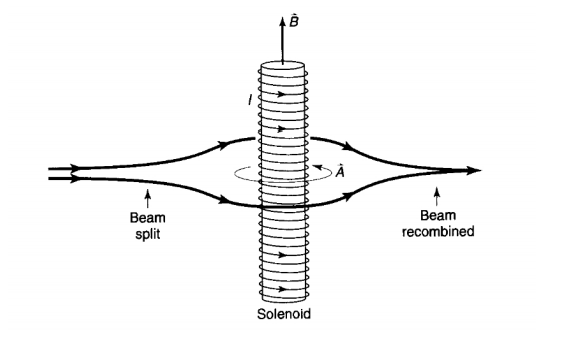
\includegraphics[scale=0.75]{bohm.png}
\end{figure}
When we turn the current on, there is a magnetic field $\mathbf{B}$ confined within the solenoid, i.e., there is no lateral magnetic field $\mathbf{B}$ on the side of the solenoid. So, according to the figure, electrons pass through a magnetic-field-free region before landing on the detector sheet. However, there exists a vector potential $\mathbf{A}$ outside of the solenoid, as the curl of $\mathbf{A}$ has to be such that the produced magnetic field $\mathbf{B}$ is contained within the coil. This can be illustrated mathematically by Stokes' theorem:
\begin{align}
\int_D \mathbf{B}\cdots \,d\mathbf{\sigma} = \int_{\sigma D}\mathbf{A}\cdot\,d\mathbf{x}.
\end{align}
The perturbed wavefunction as a result of passing through this region is
\begin{align}
\psi = \psi^0_1 e^{iS_1\hbar} + \psi^0_2 e^{iS_2/\hbar}
\end{align}
where 
\begin{align}
S_i = e\int_{\text{path } i}\mathbf{A}\cdot\,d\mathbf{x}.
\end{align}
It is clear now that the two components of the perturbed wavefunction has a phase difference of
\begin{align}
\phi = \frac{S_1-S_2}{\hbar} = \frac{e}{\hbar}\oint \mathbf{A}(\mathbf{x})\cdot\, d\mathbf{x} = \frac{e}{\hbar}\oint A^\mu\,dx_\mu,
\end{align}
which is dependent on the vector potential $\mathbf{A}$. Therefore, there is a physical effect from $\mathbf{A}$ even though the electrons do not experience any electromagnetic force. 

\subsection{Path-dependent Phase Factors}
Results from the Aharonov-Bohm experiment showed that knowing the electromagnetic field strength tensor $F^{\mu\nu}$ is not enough to determine all electrodynamic phenomena in quantum mechanics. In fact, a phase factor of the form
\begin{align}
e^{\frac{-ie}{\hbar}\oint A^\mu\,dx_\mu}
\end{align}
must be known in order to give correct predictions. Notice that the given integral is path-dependent line integral. 

\section{Phase Invariance in Field Theory}
In the previous sections we have seen somewhat of the connection between electromagnetic gauge invariance, and have generalized global phase invariance to local phase symmetry. Now, we will bring these results into Lagrangian field theory. Detailed derivations will not be focused here, as the main idea of this section is to understand what gauge transformation and symmetry are. So, we will mainly focus on results, and only derivative only when necessary. Consider the Lagrangian for the free complex scalar field: 
\begin{align}
\lag = \vert \p^\mu \phi \vert^2 = m^2\vert \psi \vert^2.
\end{align}
We will show that by the principle of least action $\phi$ and its complex conjugate satisfies the Klein-Gordon equation:
\begin{align}
(\square + m^2)\phi(x) &= 0\\
(\square + m^2)\phi^*(x) &= 0
\end{align}
Next, consider a global phase shift:
\begin{align}
\phi(x)&\to e^{iq\alpha}\phi(x)\\
\phi^*(x) &\to e^{-iq\alpha}\phi^*(x).
\end{align}
We can readily verify that the infinitesimal variations are
\begin{align}
\delta \phi &= iq(\delta \alpha)\phi\\
\delta(\p_\mu\phi) &= iq(\delta \alpha)\p_\mu\phi\\
\delta \phi^* &= -iq(\delta \alpha)\phi^*\\
\delta(\p_\mu\phi^*) &= -iq(\delta \alpha)\p_\mu\phi^*.
\end{align}
Global phase invariance requires the Lagrangian to remain unchanged, i.e.,
\begin{align}
\delta \lag = 0,
\end{align}
i.e.,
\begin{align}
\delta\lag &= \frac{\p \lag}{\p \phi}\delta \phi + \frac{\p \lag}{\p (\p_\mu\phi)}\delta (\p_\mu\phi) + \frac{\p \lag}{\p \phi^*}\delta \phi^* + \frac{\p \lag}{\p (\p_\mu\phi^*)}\delta (\p_\mu\phi^*)\\
&= \left[ \p_\mu \frac{\p \lag}{\p (\p_\mu\phi)}   \right]iq(\delta \alpha)\phi + \frac{\p\lag}{\p(\p_\mu\phi)}iq(\delta \alpha)\p_\mu\phi - (\phi\to \phi^*)\\
&= iq(\delta \alpha)\p_\mu \left[ \frac{\p\lag}{\p(\p_\mu \phi)}\phi - \frac{\p\lag}{\p(\p_\mu \phi^*)}\phi^* \right]\\ 
&\equiv 0. 
\end{align}
We can identity a conserved Noether's current (we will discuss Noether's theorem later, but the point here is to show the existence of a conserved quantity) as:
\begin{align}
J^\mu &= -iq\left[ \frac{\p\lag}{\p(\p_\mu \phi)}\phi - \frac{\p\lag}{\p(\p_\mu \phi^*)}\phi^* \right]\\
&= iq\left[\phi^*\p_\mu\phi - (\p_\mu\phi^*)\phi\right]\\
&\equiv iq\phi^*\bar{\p^\mu}\phi,
\end{align}
which satisfies
\begin{align}
\p_\mu J^\mu = 0.
\end{align}
So, we have shown the connection between global phase invariance and current conservation. But what if the transformation is local? Consider the following local phase rotation:
\begin{align}
\phi(x) \to e^{iq\alpha(x)}\phi(x).
\end{align}
The same ``problem'' arises as earlier in the section where we have some extra terms in the gradient of the scalar field:
\begin{align}
\p^\mu \phi \to e^{iq\alpha(x)}\left[ \p_\mu\phi +  iq(\p_\mu \alpha(x))\phi \right],
\end{align}
which necessitates the introduction of the gauge-covariant derivative
\begin{align}
D_\mu \equiv \p_\mu + iq A_\mu
\end{align}
such that
\begin{align}
D_\mu\phi \to e^{iq\alpha(x)}D_\mu \phi,
\end{align}
which demands the $A_\mu$ has to transform as
\begin{align}
A_\mu(x) \to A_\mu(x) - \p_\mu \alpha(x),
\end{align}
which we have verified earlier in the section. So, by requiring local phase symmetry (replacing $\p_\mu$ to $D_\mu$), we require some form of interaction between the gauge field (vector potential) $A_\mu$ and matter. 

\newpage
\chapter{Lagrangian Field Theory in Flat Spacetime}
\section{Real Scalar Fields}
A scalar field can be used to describe particles of spin 0. A scalar field has only one component, or one degree of freedom, making it the ``simplest case'' of the fields we will discuss. Let us now consider a moving field in one dimension, which has the form
\begin{align}
\phi(s) \sim e^{-i\mathbf{k}\cdot\mathbf{x}},
\end{align}
where
\begin{align}
\mathbf{k} &= K^\mu = (K^0, \vec{K})\\
\mathbf{x} &= X^\mu = (X^0, \vec{X}).
\end{align}
Remember that $K^\mu$ is the wavenumber vector, and $X^\mu$ is the position vector. Also recall that the metric is Minkowskian at this point of consideration (we are still in flat spacetime. General curved spacetime will come later):
\begin{align}
\eta_{\mu\nu} = \begin{pmatrix}
1 & 0 & 0 & 0\\
0 & -1 & 0 & 0\\
0 & 0 & -1 & 0\\
0 & 0 & 0 & -1
\end{pmatrix}.
\end{align} 
Doing the inner product of $X^\mu$ and $K^\mu$ gives
\begin{align}
\phi(x) = e^{-iK^0t + i\vec{k}\cdot\vec{x}}.
\end{align}
We shall choose ``natural units'' such that $\hbar = c = 1$. This gives
\begin{align}
\phi(x) = e^{-i\omega t}e^{i\vec{k}\cdot\vec{x}}.
\end{align}
Now, particles obey the following Einstein mass-energy equivalence:
\begin{align}
E^2 = m^2 + \vec{p}^2.
\end{align}
But because of our choice of units, $E = c\hbar K^0= K^0$, and $\vec{p} = \hbar \vec{k} = \vec{k}$. This gives
\begin{align}
\left( K^0\right)^2 - \vec{k}^2 &= m^2\\
K^\mu K_\mu &= m^2.
\end{align}
So, massive particles obey $K^\mu K_\mu = m^2$, while massless particles obey $K^\mu K_\mu = 0$. \\

Now, we might wonder how we know that the scalar field has the above form. The answer is derived from, you guessed it, the Lagrangian for a scalar field. Let us consider a single scalar field in classical mechanics where
\begin{align}
\text{Kinetic energy: } K &= \frac{1}{2}\dot{\phi}^2\\
\text{Gradient energy: } G &= \frac{1}{2}\left(\nabla \phi \right)^2\\
\text{Potential energy: } P &= V(\phi).
\end{align}
\textit{Note: I haven't found a satisfactory explanation to what a ``gradient energy'' is. I'll come back to this term later.} \\

We currently have three terms, but we would like our Lagrangian density to have the form $\mathcal{L} = K-V$. So, let us combine the kinetic energy and gradient energy terms into one:
\begin{align}
K' = \frac{1}{2}\dot{\phi}^2 - \frac{1}{2}\left(\nabla \phi \right)^2.
\end{align}
We shall verify that 
\begin{align}
K' = -\frac{1}{2}\left( \partial_\mu \phi\right)\left( \partial^\mu \phi\right) = \frac{1}{2}\dot{\phi}^2 - \frac{1}{2}\left(\nabla \phi \right)^2.
\end{align}
This turns out to be quite straightforward:
\begin{align}
\left( \partial_\mu \phi\right)\left( \partial^\mu \phi\right) &= \eta^{\mu\nu}\left( \partial_\mu \phi\right)\left( \partial_\nu \phi\right)\\
&= \left( \partial_0 \phi \right)^2 - \left(\partial_j\phi \right)^2\\
&= \dot{\phi}^2 - \left( \nabla \phi \right)^2.
\end{align}
So, a good choice of Lagrangian for our scalar field would be
\begin{align}
\mathcal{L} \sim K'-V = -\frac{1}{2}\left( \partial_\mu \phi\right)\left( \partial^\mu \phi\right) - V(\phi).
\end{align}
In order for the action to be extremized, i.e. $\delta S = 0$, we require that $\delta \mathcal{L} = 0$ for any $\delta \phi$. Varying $\mathcal{L}$ with respect to $\phi$ gives
\begin{align}
\delta \mathcal{L} &= \delta\left( -\frac{1}{2}\left( \partial_\mu \phi\right)\left( \partial^\mu \phi\right) - V(\phi)  \right)\\
&= -\frac{1}{2}\left( \partial_\mu \delta\phi\, \partial^\mu\phi + \partial_\mu\phi\,\partial^\mu\delta \phi \right) - \frac{dV(\phi)}{d\phi}\delta \phi\\
&= -\partial_\mu\delta \phi\, \partial^\mu\phi - \frac{dV(\phi)}{d\phi}\delta \phi.
\end{align}
Now, integration by parts tells us that
\begin{align}
\partial_\mu\left( \partial^\mu \phi\, \delta \phi \right) = \partial^\mu\partial_\mu\phi\, \delta \phi + \partial_\mu\delta\phi \,\partial^\mu\phi.
\end{align}
So,
\begin{align}
 \partial_\mu\delta \phi\, \partial^\mu\phi = \partial_\mu\left( \partial^\mu \phi\, \delta \phi \right) - \partial^\mu\partial_\mu\phi\, \delta \phi.
\end{align}
Therefore, variations on $\mathcal{L}$ is:
\begin{align}
\delta \mathcal{L} &= -\left[ \partial_\mu\left( \partial^\mu \phi\, \delta \phi \right) - \partial^\mu\partial_\mu\phi\, \delta \phi \right] - \frac{dV(\phi)}{d\phi}\delta \phi.
\end{align}
It follows that the action is
\begin{align}
S = \int_a^b \delta \mathcal{L}\,d^4x = \int^b_a \left\{ 
-\left[ \partial_\mu\left( \partial^\mu \phi\, \delta \phi \right) - \partial^\mu\partial_\mu\phi\, \delta \phi \right] - \frac{dV(\phi)}{d\phi}\delta \phi \right\}\,d^4x.
\end{align}
The total derivative term $\partial_\mu\left( \partial^\mu \phi\, \delta \phi \right)$ vanishes as we require the variations $\delta \phi = 0$ at $a$ and $b$. This leaves us with
\begin{align}
S = \int_a^b \left\{ 
 \partial^\mu\partial_\mu\phi - \frac{dV(\phi)}{d\phi} \right\}\,\delta \phi \,d^4x.
\end{align}
We require that this equality hold for any variation $\delta \phi$. So it must be true that
\begin{align}
\partial^\mu\partial_\mu\phi - \frac{dV(\phi)}{d\phi} = 0.
\end{align}
We introduce a new operator, the \textbf{d'Alembertian}:
\begin{align}
\square \equiv \partial^\mu\partial_\mu \equiv \partial_\nu\partial^\mu \equiv \frac{\partial^2}{\partial t^2} - \vec{\nabla}^2.
\end{align}
The requirement we just derived now becomes the \textbf{Klein-Gordon equation}:
\begin{align}
\square \phi - \frac{dV}{d\phi} = 0.
\end{align}
Remember that we are working with Lagrangian for a scalar field. It can easily be shown the connection between the Klein-Gordon equations and Newton's second law of motion, by separating the temporal and spatial derivatives from the d'Alembertian and rewriting a few things:
\begin{align}
\square \phi - \frac{dV}{d\phi} = \ddot{\phi} - \vec{\nabla}^2\phi - \frac{dV(\phi)}{d\phi} = 0.
\end{align}
We can see the time second derivative on the field $\phi$ and the $\phi$-derivative on the potential field resemble ``acceleration'' and ``force'' in Newton's second law.\\

Let us return to our original question of why a scalar field has the form $\phi  \sim e^{-i\mathbf{k}\cdot\mathbf{x}}$. From our derivation of the Klein-Gordon equation, we observe that a scalar field $\phi$ must be a solution to the Klein-Gordon equation. Now, we verify that
\begin{align}
\phi = e^{-i\mathbf{k}\cdot\mathbf{x}}
\end{align}
is a solution to the KG equation. Note that even though we are concerned with real scalar field for the time being, it is reasonable to have $\phi$ of that particular complex form, simply because it makes taking derivatives easier. One can certainly work with only the real part of $\phi$ and get the same result. Now, to check when $\phi$ satisfies the Klein-Gordon equation, we simply unpack the d'Alembertian and attack the derivatives step-by-step. The first derivative is
\begin{align}
\partial_\mu \phi &= \partial_\mu \left(e^{-i\mathbf{k}\cdot\mathbf{x}} \right)\\
&= -i\partial_\mu \left( \mathbf{k}\cdot\mathbf{x}\right)e^{-i\mathbf{k}\cdot\mathbf{x}}
\\
&= -i\partial_\mu \left(K_\nu X^\nu\right) e^{-iK_\alpha X^\alpha}\\
&= -iK_\nu\, \partial_\mu X^\nu\,\phi\\
&= -iK_\nu \delta^\nu_\mu \phi\\
&= -iK_\mu \phi 
\end{align} 
Next, we attack the second derivative:
\begin{align}
\partial^\mu \partial_\mu \phi &= \eta^{\mu\nu}\partial_\nu\partial_\mu\phi\\
&= \eta^{\mu\nu}\partial_\nu \left( -iK_\mu\phi \right)\\
&= -iK_\mu\eta^{\mu\nu}\left( -iK_\nu\phi \right)\\
&= (-i)^2 K^\mu K_\mu \phi.
\end{align}
If $K^\mu K_\mu = m^2$ (as we have shown before), then 
\begin{align}
\square \phi + m^2\phi = (-m^2 + m^2)\phi = 0, 
\end{align}
which satisfies the Klein-Gordon equation. So, as long as $K^\mu K_\mu = m^2$ is satisfied, $\phi$ of the given form is a solution to the KG equation and is a legitimate scalar field. \\

Without knowing the solution to the Klein-Gordon equation, we can also verify that the Klein-Gordon equation is the equation of motion via the Euler-Lagrange equation, which says that
\begin{align}
\frac{\p \lag}{\p \phi} - \p_\mu\left( \frac{\p \lag}{\p(\p_\mu \phi)} \right) = 0.
\end{align}
Recall the Lagrangian:
\begin{align}
\lag = \frac{1}{2}(\p_\mu\phi)(\p^\mu\phi) - V(\phi),
\end{align}
we get
\begin{align}
\frac{\p\lag}{\p\phi} &= -\frac{dV}{d\phi}\\
\frac{\p\lag}{\p(\p_\mu\phi)} &= \f{1}{2}\p^\mu\phi.
\end{align}
So the Euler-Lagrange equation gives:
\begin{align}
-\frac{dV}{d\phi} - \f{1}{2}\p_\mu(\p^\mu\phi) = 0.
\end{align}
If we reasonably take
\begin{align}
V(\phi) = \frac{1}{2}m^2\phi^2,
\end{align}
then we get $-m^2\phi - \square \phi = 0$, i.e.
\begin{align}
(\square + m^2)\phi = 0.
\end{align}



\section{Complex Scalar Fields and Electromagnetism}
\subsection{Gauge transformation of the first kind - Global Symmetry}
In this section, we will see how things ``come together.'' As real scalar fields describe massive neutral particles and how vector fields describe massless photons, complex scalar fields somehow fills in and completes the picture by bringing in the charge and somehow joins the real scalar and vector field pictures. At the end of this section, we will see how the ``full theory'' where the electromagnetic field with charge is described by a single Lagrangian. \\

If our scalar field is complex, we can think of it and its complex conjugate as:
\begin{align}
\phi &= \frac{\phi_r + i\phi_i}{\sqrt{2}}\\
\phi^* &= \frac{\phi_r - i\phi_i}{\sqrt{2}}.
\end{align}
Or, we can think of $\phi$ and $\phi^*$ as independent fields. Since the Lagrangian has to be real, plugging $\phi$ and $\phi^*$ into the Lagrangian introduced in the previous section gives:
\begin{align}
\lag = (\p_\mu \phi)(\p^\mu \phi)^* - m^2\phi^*\phi.
\end{align}
Without much inspection, we can see that the fields satisfy the Klein-Gordon equation:
\begin{align}
\begin{cases}
(\square + m^2)\phi &= 0\\
(\square + m^2)\phi^* &= 0.
\end{cases}
\end{align}
Now, we can ask ourselves: ``Is this Lagrangian invariant under the transformation
\begin{align}
\phi &\to e^{-i\Lambda}\phi\\
\phi^* &\to e^{i\Lambda}\phi^*,
\end{align}
where $\Lambda$ is a constant?'' Again, by inspection, the answer is yes, simply because the transformation is nothing but an orthogonal rotation (length preserving). And since because we changed the field the same way everywhere by a rotation induced by $e^{\pm i\Lambda}$ while the Lagrangian remains invariant, we say that the theory has a \textbf{global U(1) symmetry}. Global transformations like this one are called \textit{gauge transformation of the first kind}.
\subsection{Gauge transformation of the second kind - Local Symmetry}
Now, consider the case where the rotation operation $e^{\pm i \Lambda}$ has a spatio-dependence, i.e., $\Lambda \to \Lambda(x)$. We call this a \textit{gauge transformation of the second kind}. This leads to the fact that $\phi$ transform differently at different places. We want our theory to also be invariant under this ``local'' transformation. But first, we have to show that our previous Lagrangian no longer retains its gauge symmetry and try to come up with ways to ``fix'' the theory. Let us say that $\phi$ transforms as $\phi \to \phi e^{i\Lambda(x)}$, then
\begin{align}
\p_\mu \phi \to \p_\mu (\phi e^{i\Lambda(x)}) = i(\p_\mu \Lambda(x))\phi + e^{i\alpha}\p_\mu \phi.
\end{align}
It is already clear that 
\begin{align}
(\p_\mu \phi)(\p_\mu \phi)^* \not\to (\p_\mu \phi)(\p_\mu \phi)^* e^{i\Lambda(x)}
\end{align}
since there will always be some $\Lambda(x)$-dependent residual terms. We can stop here and surrender, but we can also ``fix'' our notion of the derivative (just like what we did in general relativity), introducing the \textbf{gauge-covariant derivative}:
\begin{align}
D_\mu = \p_\mu + iqA_\mu,
\end{align}
where $q$ is the charge, which acts as a \textit{coupling term} like the Christoffel symbols in general relativity, and $A_\mu$ is the vector potential, which is also the gauge field that has symmetry:
\begin{align}
A_\mu \sim A_\mu + \p_\mu\Lambda.
\end{align}
Once again, recall we have discussed in the gauge invariance section. By adding the 4-dimensional gradient of a scalar field $\Lambda$ (so adding the $\p_\mu \Lambda$ term), we are not changing the 4-dimensional curl of $A_\mu$, i.e. the electromagnetic field tensor $F^{\mu\nu}$ is divergence-free. We can refer to section on gauge invariance for more details about this is true. But focusing on the results here, if we cleverly (once again) pick $\Lambda$ such that
\begin{align}
\Lambda(x) = -\frac{\alpha(x)}{q}
\end{align}
then with the gauge transformations
\begin{align}
\begin{cases}
\phi \to \phi e^{i\Lambda(x)}\\
A_\mu \to A_\mu - \frac{1}{q}\p_\mu\Lambda(x)
\end{cases}
\end{align}
the new derivative $D_\mu\phi = (\p_\mu + iqA_\mu)\phi$ is transformed into
\begin{align}
&\to \left( \p_\mu  iq\left[ A_\mu -\frac{1}{q}\p_\mu\Lambda(x)  \right] \right)\phi e^{i\Lambda(x)}\\
&= e^{i\Lambda(x)}\left( \p_\mu\phi + i(\p_\mu\Lambda(x)\phi) + iqA_\mu \phi - i(\p_\mu \Lambda(x))\phi \right)\\
&= e^{i\Lambda(x)}(\p_\mu \phi + iqA_\mu\phi)\\
&= e^{i\Lambda(x)}D_\mu\phi.
\end{align}
So, $D_\mu\phi$ transforms correctly. Since we have added the electromagnetic vector potential to the theory, adding the electromagnetic field tensor term completes the classical field theory for the charged scalar field in electromagnetism. 
\begin{align}
\boxed{\lag = \vert D_\mu \phi\vert^2 - m^2\vert \phi\vert^2 - \frac{1}{4}F_{\mu\nu}F^{\mu\nu} }
\end{align}
In the next section, we will look at the underlying motivations for the choices we have made regarding ``fixing'' our notion of the derivatives and $\Lambda$.


\subsection{Motivations in the derivation of the E\&M Lagrangian}
In the previous section, we have look at the basics of gauge transformations and global and local symmetry. We have also come across a number of ``clever'' choices, but those choices have so far been unjustified. in this section, we will try to develop an understanding for ``why'' the complete Lagrangian of electromagnetism and matter has the following form
\begin{align}
\lag = \vert D_\mu \phi\vert^2 - m^2\vert \phi\vert^2 - \frac{1}{4}F_{\mu\nu}F^{\mu\nu} .
\end{align} 

First, we revisit the gauge transformation of the second kind, i.e., local gauge transformation where
\begin{align}
\phi \to \phi' = e^{i\Lambda(x)}\phi \approx (1-i\Lambda(x))\phi
\end{align}
for $\Lambda(x) \ll 1$. Variations on the field give
\begin{align}
\delta \phi &= -i\Lambda \phi
\end{align}
and
\begin{align}
\p_\mu \phi &\to \p_\mu \phi - i(\p_\mu\Lambda(x))\phi - i\Lambda(x)(\p_\mu \phi).
\end{align}
Therefore
\begin{align}
\delta(\p_\mu\phi) = -i\Lambda(\p_\mu\phi) - i(\p_\mu\Lambda)\phi.
\end{align}
We can do the same with the complex conjugate of $\phi$, giving
\begin{align}
\delta \phi^* &= i\Lambda \phi^*\\
\delta(\p_\mu\phi^*) &= i\Lambda(\p_\mu\phi^*) +  i(\p_\mu\Lambda)\phi^*.
\end{align}
Assuming that the Lagrangian for electromagnetism takes the form like that of the massive scalar field case:
\begin{align}
\lag = (\p_\mu\phi)(\p^\mu\phi^*) - m^2\phi^*\phi,
\end{align}
variations on the Lagrangian gives
\begin{align}
\delta \lag &= \delta[(\p_\mu\phi)(\p^\mu\phi^*)] - m^2 \delta(\phi^*\phi)\\
&= [\delta(\p_\mu\phi)](\p^\mu\phi^*) + (\p_\mu\phi)[\delta(\p^\mu\phi^*)] - m^2[(\delta \phi)\phi^* + \phi(\delta \phi^*)].
\end{align}
We can readily verify that $(\delta \phi)\phi^* + \phi(\delta \phi^*)$ is zero by the above identities:
\begin{align}
(\delta \phi)\phi^* + \phi(\delta \phi^*)&= -i\Lambda \phi \phi^* + \phi i\Lambda \phi^* = 0.
\end{align}
So we're left with
\begin{align}
\delta \lag&= [-i\Lambda(\p_\mu\phi) - i(\p_\mu\Lambda)\phi](\p^\mu\phi^*) + (\p_\mu\phi)[i\Lambda(\p_\mu\phi^*) +  i(\p_\mu\Lambda)\phi^*]\\
&= -i\Lambda(\p_\mu\phi)(\p^\mu\phi^*) - i(\p_\mu\Lambda)\phi (\p^\mu\phi^*)\\ 
&\,\,\,\,\,\,\,\,\,\,+ i\Lambda (\p^\mu\phi^*)(\p_\mu\phi) + i\phi^*(\p^\mu\Lambda)(\p_\mu\phi)\\
&= i\phi^*(\p^\mu\Lambda)(\p_\mu\phi) - i(\p_\mu\Lambda)\phi (\p^\mu\phi^*)\\
&= i\phi^*(\p_\mu\Lambda)(\p^\mu\phi) - i(\p_\mu\Lambda)\phi (\p^\mu\phi^*)\\
&= (\p_\mu\Lambda)[i\phi^*\p^\mu\phi - i\phi\p^\mu\phi^*].
\end{align}
By Noether's theorem, which we will into much more detail in the following sections:
\begin{align}
J^\mu &= \frac{\p\lag}{\p(\p_\mu\phi)}(-i\phi) + \frac{\p\lag}{\p(\p_\mu\phi^*)}(i\phi^*)\\
&= i(\phi^*\p^\mu\phi - \phi\p^\mu\phi^*).
\end{align}
So the variation in the Lagrangian becomes
\begin{align}
\delta \lag &= (\p_\mu\Lambda)J^\mu. 
\end{align}
Now, our ultimate goal is achieve some sort of invariance. But by the look of $\delta \lag$ we are already failing to have invariance. However, we can fix this, by adding terms to the Lagrangian such that this $J^\mu$ term goes away (this is exactly the idea of \textit{gauge invariance} which we have discussed earlier). So, consider
\begin{align}
\lag_1 &= -eJ^\mu A_\mu\\
&= -e[i\phi^*\p^\mu\phi - i\phi\p^\mu\phi^*]A_\mu.
\end{align}
where we have introduced the vector potential $A_\mu$. Recall in the section on gauge invariance we have require $A_\mu$ to transform as
\begin{align}
A'_\mu&= A_\mu + \frac{1}{e}\p_\mu\Lambda
\end{align}
in order to achieve gauge invariance. (Note that there is a subtle sign change due to different sign conventions, but the idea is the same). Thus variations on $A_\mu$ is given by
\begin{align}
\delta A_\mu = A'_\mu - A_\mu = \frac{1}{e}\p_\mu\Lambda
\end{align}

Plug this into the variation of this extra term $\lag_1$ we get
\begin{align}
\delta \lag_1&=-\delta[eJ^\mu A_\mu]\\
&= -e(\delta J^\mu)A_\mu -eJ^\mu(\delta A_\mu)\\
&= -e(\delta J^\mu)A_\mu - J^\mu\p_\mu\Lambda
\end{align}
We shall compute $\delta J^\mu$ here:
\begin{align}
\delta J^\mu &= i\delta  (\phi^*\p^\mu\phi - \phi\p^\mu\phi^*)\\
&= i[(\delta\phi^*)\p^\mu\phi + \phi^*\p^\mu(\delta\phi)- \phi(\p^\mu\delta\phi^*) - (\delta\phi)\p^\mu\phi^*]\\
&= i[i\Lambda\phi^*\p^\mu\phi - \phi^*\p^\mu (i\Lambda \phi)- \phi\p^\mu (i\Lambda\phi^*) + i\Lambda\phi\p^\mu\phi^*]\\
&= -\Lambda\phi^*\p^\mu\phi + \phi^*\p^\mu (\Lambda \phi) + \phi\p^\mu (\Lambda\phi^*) - \Lambda\phi\p^\mu\phi^*\\
&= -\Lambda\phi^*\p^\mu\phi + \Lambda\phi^*\p^\mu\phi + \phi^*\phi\p^\mu\Lambda + \phi \Lambda \p^\mu\phi^* + \phi \phi^*\p^\mu\Lambda - \Lambda\phi\p^\mu\phi^*\\
&= 2\phi^*\phi \p^\mu\Lambda.
\end{align}
So, variations on the modified Lagrangian is now
\begin{align}
\delta \lag + \delta \lag_1 &= (\p_\mu\Lambda)J^\mu -e(2\phi^*\phi\p^\mu\Lambda) - J^\mu(\p_\mu\Lambda)\\
&=  -2eA_\mu\phi^*\phi(\p^\mu\Lambda).
\end{align}
But it looks like we are \textit{still} achieving invariance. So, we have to repeat the procedure, adding more terms to the Lagrangian. Let's call this additional term $\lag_2$, defined as
\begin{align}
\lag_2 = e^2 A_\mu A^\mu\phi^*\phi.
\end{align}
Varying $\lag_2$ gives
\begin{align}
\delta \lag_2 &= \delta(e^2 A_\mu A^\mu\phi^*\phi)\\
&= e^2 \phi^*\phi A_\mu\delta A^\mu + e^2 \phi^*\phi A^\mu\delta A_\mu\\
&= 2e^2A_\mu(\p^\mu \Lambda)\phi^*\phi.
\end{align}
Now, we should achieve invariance:
\begin{align}
\delta \lag + \delta \lag_1 + \delta \lag_2 &= -2eA_\mu\phi^*\phi(\p^\mu\Lambda) + 2e^2A_\mu(\p^\mu \Lambda)\phi^*\phi\\
&= 0.
\end{align}
The total Lagrangian $\lag + \lag_1 + \lag_2$ is now invariant under local gauge transformation, but at the price of introducing the vector potential $A_\mu$, which couples to the current $J_\mu$ of the complex $\phi$ field. Now, $A_\mu$ must also be contributing to the Lagrangian, so we need to take into account for that contribution by requiring an additional (invariant) term that involves nothing but the electromagnetic field strength tensor:
\begin{align}
\lag_3 = -\frac{1}{4}F^{\mu\nu}F_{\mu\nu}.
\end{align}
So, the total Lagrangian becomes:
\begin{align}
\lag_{\text{tot}} &= \lag+ \lag_1 + \lag_2 + \lag_3\\
&= (\p_\mu\phi)(\p^\mu\phi^*) -ie(\phi^*\p^\mu\phi - \phi\p^\mu\phi^*)A_\mu\\
&\,\,\,\,\,\,\,\,\,\, e^2A_\mu A^\mu \phi^*\phi - m^2 \phi*\phi - \frac{1}{4}F^{\mu\nu}F_{\mu\nu}.
\end{align}
Some simplification gives
\begin{align}
\lag_{\text{tot}} = (\p_\mu\phi + ieA_\mu\phi)(\p^\mu\phi^* - ieA^\mu\phi^*) - m^2\phi^*\phi - \frac{1}{4}F^{\mu\nu}F_{\mu\nu}.
\end{align}
Now, the form of the Lagrangian is starting to look like the Lagrangian we wish to achieve in the beginning of this section. Indeed, we can see that our derivative has been slightly modified to include the vector potential:
\begin{align}
\p_\mu \to \p_\mu + ieA_\mu.
\end{align}
So we if define a new operator
\begin{align}
D_\mu = \p_\mu + ieA_\mu,
\end{align}
then we see that it is indeed invariant under local gauge transformations (as already been shown numerous times in this text). It is worthwhile, however, to show again, but in a slightly different light:
\begin{align}
\delta(D_\mu\phi) &= \delta(\p_\mu\phi) + ie(\delta A_\mu)\phi + ieA_\mu\delta \phi\\
&= -i\Lambda (\p_\mu\phi + ieA_\mu\phi)\\
&= -i\Lambda (D_\mu\phi).
\end{align}
In fact, this is true even without the approximation $\Lambda \ll 1$. To show this, we also have to take into account the transformation of $A_\mu \to A'_\mu$, i.e., the operators are not the same at different locations in space. But it can easily be done. In fact, we have shown this in the section on gauge invariance. \\

Now, we are getting really close to coming a full circle to justify the numerous of ``clever choices'' in the previous sections. However, we shall still be careful and look at a subtle difference:
\begin{align}
D_\mu \equiv \p_\mu + ieA_\mu
\end{align}
if applied to the scalar field $\phi$, while 
\begin{align}
D_\mu \equiv \p_\mu -ieA_\mu
\end{align}
if applied to the complex conjugate scalar field $\phi^*$. But the operator itself shouldn't know in advance what kind of function is being fed to it so that it can change accordingly. Also, the role of ``complex conjugate'' is exchangeable, thus a ``sign-varying'' definition of $D_\mu$ certainly does not work. To resolve this, we must recognize this: because $e$ is the electric charge, changing the sign of $e$ changes the sign of the charge. Now, because this goes hand-in-hand with the field $\phi$ and its complex conjugate $\phi^*$, i.e., whenever we have the complex conjugate, the sign of $e$ in the operator changes, we might as well associate the field $\phi$ with having the charge $e$, and the field $\phi^*$ with having the charge $-e$. To summarize, we simply note: $\phi$ describes a field with charge $e$, and $\phi^*$ describes a field with charge $-e$. So, we can now be satisfied with the Lagrangian for electromagnetism and classical field theory (in flat spacetime):
\begin{align}
\boxed{ \lag = (D_\mu\phi)(D^\mu\phi^*) - m^2 A_\mu A^\mu - \frac{1}{4}F^{\mu\nu}F_{\mu\nu}}
\end{align}

\subsection{A few remarks}
Here are a few key concepts we should clarify and make sure we understand correctly. These can be treated as important takeaways from this section. It also helps to have some ``intuitive'' grounding and a good ``narrative'' in mind when we talk about the theory. Sometimes, while the mathematics is straightforward, it can be tremendously difficult to interpret a theory and ``understand'' it. So, while not as technical as the other sections, this subsubsection serves to summarize and hopefully explain why we did what we have done and defined what we have defined. I hope this section sort of ``brings everything together'' before we move on to other topics. 
\begin{enumerate}
	\item $D_\mu\phi^*$ is a covariant derivative of $\phi^*$ not because we conjugated $D_\mu\phi$ but because it transforms in the same way that $\phi^*$ does under gauge transformations. We can readily verify this (in fact, we have verified this many times). 
	\item How can we be sure that $A_\mu$ is actually the vector potential? This is possibly a question that a careful reader would ask right from the beginning. But no worries, as we know for sure that $A_\mu$ must be the (compensating) vector potential. Why? Because of the definition of the electromagnetic field strength tensor as the 4-dimensional curl of $A_\mu$. 
	\item As a result of the previous item, we have a new interpretation for the electromagnetic field: The electromagnetic field is the gauge field which has to be introduced to guarantee invariance under local U(1) gauge transformations. 
	\item The Maxwell's inhomogeneous equations (i.e., not in a vacuum, i.e., there exists some current $\mathcal{J}^\mu$) arise as a result of varying the vector potential $A_\mu$, i.e., by requiring that $A_\mu$ satisfy the Euler-Lagrange equation for $A_\mu$:
	\begin{align}
	\frac{\p\lag}{\p A_\mu} - \p_\nu \left( \frac{\p\lag}{\p(\p_\nu A_\mu)} \right) = 0
	\end{align}
	where the Lagrangian is what we just derived
	\begin{align}
	\lag &= (D_\mu\phi)(D^\mu\phi) - m^2 A_\mu A^\mu - \frac{1}{4}F^{\mu\nu}F_{\mu\nu} \\
	&= (\p_\mu\phi + ieA_\mu\phi)(\p^\mu\phi^* - ieA^\mu\phi^*) - m^2\phi^*\phi - \frac{1}{4}F^{\mu\nu}F_{\mu\nu}
	\end{align}
	we obtain (which the unconvinced and diligent reader can and should readily verify by attacking the Lagrangian with derivatives)
	\begin{align}
	\p_\nu F^{\mu\nu} &= -ie(\phi^*\p^\mu\phi - \phi\p^\mu\phi^*) + 2e^2A^\mu\vert \phi\vert^2\\
	&= -ie(\phi^* D^\mu\phi - \phi D^\mu\phi^*)\\
	&= -e\mathcal{J}^\mu,
	\end{align}
	where the definition of the \textbf{covariant current} $\mathcal{J}^\mu$
	\begin{align}
	\mathcal{J}^\mu \equiv \phi^* D^\mu\phi - \phi D^\mu\phi^*
	\end{align} is ``covariantly motivated'' by the definition of $J^\mu$. Now, because
	\begin{align}
	\p_\mu (\p_\nu F^{\mu\nu}) &= \p_\mu\p_\nu (\p^\mu A^\nu - \p^\nu A^\mu)\\
	&= \p_\mu\p_\nu\p^\mu A^\nu - \p_\mu\p_\nu\p^\nu A^\mu\\
	&= \p_\mu\p_\nu\p^\mu A^\nu - \p_\nu\p_\mu\p^\mu A^\nu\\
	&= 0,
	\end{align}
	it must also be true that
	\begin{align}
	\p_\mu \mathcal{J}^\mu = 0,
	\end{align}
	i.e., the covariant current is \textbf{conserved} when the electromagnetic field is present, NOT the current $J^\mu$.
	\item We have shown very early in the section that the electromagnetic field is \textbf{massless}, but it is worth emphasizing this point. If we add the mass term:
	\begin{align}
	\lag_M = M^2A_\mu A^\mu
	\end{align}
	to the Lagrangian, we no longer get invariance under gauge transformation. This means that \textit{gauge invariance requires the electromagnetic field - the gauge field - to be massless}. This turns out to be very important particle physics. 
	\item What does the charge $e$ do in the theory? We can indeed think of $e$ as a coupling constant, as we have discussed. If we look at the Lagrangian, we can see clearly that the field $\phi$ couples to the electromagnetic field with strength $e$. So, it seems that the electric charge plays \textbf{two roles} in theory: (i) measuring the strength with which a particle interacts with electric and magnetic fields, and (ii) serves as a conserved quantity. These two roles in fact arise as a consequence of the ``gauge principle,'' which is also very important in particle physics. 
\end{enumerate}




\section{Vector Fields and Photons}
In this section, we will see how electromagnetism naturally arises from the previous section where we demand invariance of the action under gauge transformation of the second kind (local rotations). In particular, we will work with a Lagrangian density that describes the massless and neutral photon, and see how variations on the action gives rise to the Maxwell's equations. We will also confirm that fact that photons must be massless in the theory, by enforcing conditions on the vector potential $A_\mu$. The section is more of synopsis of the methods we have learned so far about variations on the action, gauge transformations, symmetries, and invariances. The goal of this section is to show the theory actually works to describe a physical, real, particle. We will be working with vector field in the formulation the action, but the main principles regarding variations and gauge-stuff are the same.  \\

Vector fields describe particles of spin 1 such as photons. Unlike real scalar fields $\phi$ where there is only one degree of freedom, a vector field is represented by $A_\mu$ with $\mu = 0,1,2,3$, hence having 4 degrees of freedom. Electromagnetism is a field theory where the relevant field is a vector field, $A_\mu$, called the vector potential.
\begin{align}
A_\mu = (A_0, \vec{A}).
\end{align}
The first component of the vector potential, $A_0$ is the electrostatic potential $V$ where $\vec{E} = -\vec{\nabla}V$. The other spatial components of $A_\mu$, forming $\vec{A}$, form the vector potential from which the magnetic field and full electric field is derived:
\begin{align}
\vec{B} &= \vec{\nabla}\times \vec{A}\\
\vec{E} &= -\vec{\nabla}V - \frac{\partial \vec{A}}{\partial t}
\end{align}

Let us consider the following Lagrangian density:
\begin{align}
\mathcal{L} = -\frac{1}{4}F_{\mu\nu}F^{\mu\nu} - j^\mu A_\mu,
\end{align}
where $j^\mu = (\rho, \vec{J})$ is a combination of the charge density and current density. The electromagnetic field strength tensor is given by:
\begin{align}
F^{\mu\nu} &= \partial^\mu A^\nu - \partial^\nu A^\mu \\
&= \begin{pmatrix}
0 & -E^1 & -E^2 & -E^3\\
E^1 & 0 & -B^3 & B^2 \\
E^2 & B^3 & 0 & -B^1\\
E^3 & -B^2 & B^1 & 0
\end{pmatrix}.
\end{align}
With this definition, we can also have an equivalent definition:
\begin{align}
F_{\mu\nu} = \partial_\mu A_\nu - \partial_\nu A_\mu.
\end{align}
Recall the cyclic identity (this can be readily verified - we in fact have covered this in the GR notes):
\begin{align}
\partial_\lambda F_{\mu\nu} + \partial_{\mu}F_{\nu\lambda} + \partial_{\nu}F_{\lambda\mu} = 0.
\end{align}
We can easily show that this identity yields two of four Maxwell's equations:
\begin{align}
\vec{\nabla}\times\vec{E} &= -\frac{\partial \vec{B}}{\partial t}\\
\vec{\nabla}\cdot\vec{B} &= 0.
\end{align}
The remaining Maxwell equations come from varying the action and minimizing the action: $\delta S = 0$ with respect to the vector potential $A_\mu$. Similar to what we have done before, we want to vary the Lagrangian. Now, the E\&M Lagrangian has two terms. The term involving the vector potential is simple:
\begin{align}
\delta \left( j^\mu A_\mu \right) = j^\mu\,\delta A_\mu 
\end{align}
true for all $\delta A_\mu$, so if the field strength tensor is zero, then $j^\mu = 0$. The term involving the field strength tensor is a little more complicated, but certainly doable:
\begin{align}
\delta\left( \frac{-1}{4}F^{\mu\nu}F_{\mu\nu} \right) 
&= \frac{-1}{4}\,\delta\left[\left( \partial^\mu A^\nu - \partial^\nu A^\nu  \right)\left( \partial_\mu A_\nu - \partial_\nu A_\mu \right)\right]\\
&= \frac{-1}{2}\,\delta\left( \partial^\mu A^\nu\,\partial_\mu A_\nu - \partial_\mu A_\nu\,\partial^\mu A^\nu\right)\\
&= \frac{-1}{2}\left( \partial^\mu\,\delta A^\nu\,\partial_\mu A_\nu  + 
\partial^\mu A^\nu\,\partial_\mu\,\delta A_\nu - \partial_\mu \,\delta A_\nu\,\partial^\mu A^\nu - \partial_\mu  A_\nu\,\partial^\mu \,\delta A^\nu \right).
\end{align}
Raising and lowering indices gives
\begin{align}
\delta\left( \frac{-1}{4}F^{\mu\nu}F_{\mu\nu} \right)  
&= \frac{-1}{2}\left( 
\partial^\mu\,\delta A^\nu\,\partial_\mu A_\nu  + 
\partial_\nu A_\mu\,\partial^\nu\,\delta A^\mu 
- \partial_\mu \,\delta A_\nu\,\partial^\mu A^\nu 
- \partial^\nu A^\mu\,\partial_\nu \,\delta A_\mu \right)\\
&= \partial^\nu\,\delta A^\mu\,\partial_\nu A_\mu - \partial_\mu \,\delta A_\nu\,\partial^\mu A^\nu.
\end{align}
We can again integrate by parts on the two terms similar to the following steps
\begin{align}
\partial^\nu\,\delta A^\mu\,\partial_\nu A_\mu &=  \partial^\nu(\partial_\mu A_\nu\,\delta A^\mu) -(\partial^\nu\partial_\mu A_\nu)\delta A^\mu = \partial_\mu(\partial^\nu A^\mu\,\delta A_\nu) -(\partial^\nu\partial_\mu A_\nu)\delta A^\mu
\\
\partial_\mu\,\delta A_\nu\partial^\mu A^\nu &= 
\partial_\mu (\partial^\mu A^\nu \,\delta A_\nu)
 - \partial_\mu(\partial^\mu A^\nu)\,\delta A_\nu  =
\partial_\mu (\partial^\mu A^\nu \,\delta A_\nu) 
 - \partial_\mu(\partial^\mu A^\nu)\,\delta A_\nu.
\end{align} 
and eliminate the total derivative from the action integral. Assuming that the term with the current density and vector potential is zero, we are eventually (after lowering/raising the indices correctly, of course) left with the requirement
\begin{align}
\partial_\mu(\partial^\mu A^\nu)\,\delta A_\nu - (\partial^\nu\partial_\mu A_\nu)\delta A^\mu
&\equiv 
\left(\square A^\mu - \partial^\mu\partial^\nu A_\nu \right)\,\delta A_\mu = 0
\end{align}
for all $\delta A_\mu$, which forces the following identity:
\begin{align}
\square A^\mu - \partial^\nu \partial^\mu A_\nu = \square A^\mu - \partial_\nu \partial^\mu A^\nu = \partial_\nu(\partial^\nu A^\mu - \partial^\mu A^\nu) = \partial_\nu F^{\mu\nu} = 0.
\end{align}
Now, with the current density and vector potential terms, we get the requirement 
\begin{align}
\partial_\nu F^{\mu\nu} = j^\mu. 
\end{align}
This identity gives the remaining two Maxwell's equations.\\

We can look at photons as an example. Photons do not carry a current/charge, so $j^\mu = 0$. Therefore the equation of motion can be derived from just
\begin{align}
\partial_\nu F^{\mu\nu} = 0.
\end{align}
Now, we have an interesting problem to think about: We know that photons can have 2 independent transverse polarizations, i.e. there are 2 massless modes for photons. However, $A^\mu$ has 4 degrees of freedom, not 2. So why does our theory require more than 2 degrees of freedom to describe a physical quantity that only has 2 degrees of freedom? The answer to this is that there are 2 degrees of freedom in $A_\mu$ that don't matter. The first is the $A_0$ factor - the electrostatic potential. Why $A_0$ does not matter in describing photons can be illustrated if we look at the case where $\mu = 0$:
\begin{align}
\square A_0 - \partial_0\,\partial^\nu A_\nu 
&= \partial^0\partial_0A_0 + \partial^j\partial_jA_0 - \partial_0\partial^0A_0-\partial_0\partial^jA_j\\ 
&=  \partial^j\partial_jA_0 - \partial_0\partial^jA_j \\
&=  0.
\end{align} 
We see that $A_0$ is not a propagating mode, or the \textbf{ghost} mode, or the \textbf{auxiliary} mode. This is actually a good thing in our theory. In fact, the Lagrangian is actually chosen such that the time second derivative vanishes. \\

Now that we have sort of explained why one degree of freedom of $A_\mu$ does not matter. What about the other one that shouldn't matter? The short answer to this is the keyword \textbf{gauge symmetry} in the theory. If we look back at how the field strength tensor is defined as the 4-dimensional curl of the vector potential $A_\mu$:
\begin{align}
F_{\mu\nu} = \partial_\mu A_\nu - \partial_\nu A_\mu.
\end{align}
As an aside, it makes sense to define the 4-dimensional curl this way, because the curl of a 2-vector field in two dimensions gives a scalar (a zero-index object), the curl of a 3-vector field in three dimensions gives a 3-vector field (a one-index object). So it is reasonable to define the 4-dimensional curl of a 4-vector field as a tensor (a two-index object). Now, back to our problem. We should also attempt to gauge transform
\begin{align}
A_\mu \rightarrow A'_\mu = A_\mu + \partial_\mu\Lambda(x),
\end{align}
then we observe that
\begin{align}
F'_{\mu\nu} &= \partial_\mu(A_\nu + \partial_\nu\Lambda(x)) - \partial_\nu(A_\mu + \partial_\mu\Lambda(x))\\
 &= \partial_\mu A_\nu - \partial_\nu A_\mu \\
 &= F^{\mu\nu},
\end{align}
i.e. there is a way to choose $\Lambda(x)$ such that we eliminate one $A_\mu$ mode, leaving just 4-1-1=2 modes.\\

The goal of the above gauge transformation is to pick a $\Lambda(x)$ to remove an extra degree of freedom in the theory. Let us suppose that $\p^\mu A_\mu \neq 0$, i.e. $A_\mu$ is NOT divergence-free. We can pick $\Lambda(x)$ such that after the transformation, $\p^\mu A'_\mu = 0$. Let's start from the very beginning, repeat what we just done earlier:
\begin{align}
A'_\nu = A_\nu + \p_\nu\Lambda.
\end{align}
It follows that
\begin{align}
\p^\nu A'_\nu &= \p^\nu(A_\nu + \p_\nu\Lambda)\\
&= \p^\nu A_\nu + \p^\nu \p_\nu \Lambda\\
&= \p^\nu A_\nu + \square\Lambda.
\end{align}
This suggests that if we pick $\Lambda(x)$ such that $\square\Lambda(x) = -\p^\nu A_\nu$ then in this gauge $\p^nu A'_\nu = 0$. After that, we can just drop the prime and get $\p^\nu A_\nu = 0$. As a consequence, in this fixed gauge, the equations of motion can be deduced from 
\begin{align}
\begin{cases}
\square A_\mu = 0\\
\p^\nu A_\nu = 0
\end{cases}
\end{align}
each of which adds one constraint, reducing the degree of freedom by 1. To solve for $A_\mu$, we can assume the form of $A_\mu$:
\begin{align}
A_\mu = \epsilon_\mu e^{-i\mathbf{k}\cdot\mathbf{x}},
\end{align}
where $\epsilon_\mu$ is called the \textbf{polarization vector}. Now, let us work with the first constraint $\square A = 0$. We can verify (below) that this constraint requires $K^\mu K_\mu = 0$, i.e. $K^\mu$ is a null vector in flat Minkowskian spacetime, i.e. it is light-like. 
\begin{align}
\square A_\mu &= \p_\mu \p^\mu A_\mu\\
&= \p_\mu\left( 
\eta^{\mu\nu}\p_\nu \epsilon_\mu e^{-i\mathbf{k}\cdot\mathbf{x}}
\right)\\
&= \p_\mu\left[\epsilon_\mu\eta^{\mu\nu}\left(\p_\nu  e^{-i\mathbf{k}\cdot\mathbf{x}}
\right)\right]\\
&= \p_\mu\left[\epsilon_\mu\eta^{\mu\nu}(-iK_\mu)\left(
e^{-i\mathbf{k}\cdot\mathbf{x}}\p_\nu X^\mu
\right)\right]\\
&= \p_\mu\left[\epsilon_\mu\eta^{\mu\nu}(-iK_\mu)\left(
e^{-i\mathbf{k}\cdot\mathbf{x}}\delta^\mu_\nu
\right)\right]\\
&= (-iK^\nu)\p_\mu A_\mu\\
&= 4(-iK^\nu)(-iK_\mu)A_\mu\\
&= 4(-i)^2 K_\mu K^\mu A_\mu\\
&= 0 \text{ if } K_\mu K^\mu = 0.
\end{align}
This requirement implies that the vector field $A_\mu$ is massless ($K^\mu K_\mu = 0$ rather than $m^2$ like in the scalar field example), which is a good thing, since we are working with electromagnetism and these mathematical objects ultimately describe electromagnetic waves - photons. \\

Next, the other constraint $\p^\nu A_\nu = 0$ motivates us to choose $\Lambda$ such that
\begin{align}
\square \Lambda = -\p^\nu A_\nu
\end{align}
so that $\p^\nu A'_\nu = 0$. However, this isn't enough information to choose $\Lambda$, because $\square \Lambda = -\p^\nu A_\nu$ alone cannot fix $\Lambda$. We also have to look at the gauge transformation of $A_\mu$ and make sure that the auxiliary part $A_0$ vanishes, then we have enough information to pick $\Lambda$. Let us start with the form of $A_\mu$:
\begin{align}
A_\mu = \epsilon_\mu e^{-i\mathbf{k}\cdot\mathbf{x}}.
\end{align}
We know that $\square A_\mu = 0$, so if we pick
\begin{align}
\Lambda = \lambda e^{-i\mathbf{k}\cdot\mathbf{x}}
\end{align}
then we are guaranteed $\square \Lambda = 0 = \p^\nu A_\nu$. So that is quite nice. But what is $\lambda$? We can only set $\lambda$ if we fix the value of $A_0$. It makes sense to set $A_0 = 0$ so that it vanishes. With this, we can perform a gauge transformation on $A_0$, set it to zero, and find $\lambda$:
\begin{align}
A_0 &\rightarrow A_0 + \p_0 \Lambda = 0\\
&\rightarrow e^{-i\mathbf{k}\cdot\mathbf{x}}(\epsilon_0 - i\lambda K_0) = 0\\
&\rightarrow \lambda = \frac{\epsilon_0}{i K_0}. 
\end{align}
So, if we pick 
\begin{align}
\Lambda = \frac{\epsilon}{i K_0}e^{-i\mathbf{k}\cdot\mathbf{x}}
\end{align}
then $A_0 = 0$ implies
\begin{align}
\p^\nu A_\nu = \p^0 A_0 + \vec{\nabla}\cdot\vec{A} = \vec{\nabla}\cdot\vec{A} = 0.
\end{align}
So, it turns out that we can simply complete gauge fixing by setting two additional constraints on $A_\mu$:
\begin{align}
\begin{cases}
A_0 = 0\\
\vec{\nabla}\cdot\vec{A} = 0,
\end{cases}
\end{align}
i.e., we require that the vector potential $A_\mu$ be divergence-free and to have a vanishing auxiliary mode. With this, we can the degree of freedom of $A_\mu$ from 4 from 2, making it a physical description. We shall show that can be done now. If we revisit the polarization vector
\begin{align}
\epsilon_\mu = (\epsilon_0, \epsilon_1, \epsilon_2, \epsilon_3)
\end{align}
and require that $A_0 = 0$, then obviously $\epsilon_0 = 0$. But since we also require $\vec{\nabla}\cdot\vec{A} = 0$, we have
\begin{align}
\vec{\nabla}\cdot\vec{A} &= \p_j A^j\\
&= \p_j \left( \epsilon^j e^{-i\mathbf{k}\cdot\mathbf{x}} \right)\\
&\propto A^j (-iK_j)\\
&= 0.
\end{align}
So, $\vec{k}\cdot\vec{A} = 0$, i.e., they are orthogonal vectors. Now, consider a photon traveling in the $z$-direction. Because $K_\mu k^\mu = 0$, we have
\begin{align}
K^\mu = (K,0,0,K).
\end{align}
Because $\vec{k}\cdot\vec{A} \propto \vec{k}\cdot\vec{\epsilon}$, it follows that $K\epsilon^3 = 0$, i.e., there is no longitudinal component in the polarization vector. Therefore,
\begin{align}
\epsilon_\mu = (0, \epsilon_1, \epsilon_2, 0).
\end{align}
So, the vector potential $A_\mu$ has the form
\begin{align}
A_\mu = \epsilon_\mu e^{-i\mathbf{k}\cdot\mathbf{x}} = \begin{pmatrix}
0\\\epsilon_1\\\epsilon_2\\0
\end{pmatrix}e^{-i\mathbf{k}\cdot\mathbf{x}}.
\end{align}
We can construct the independent modes of propagation as
\begin{align}
\begin{cases}
\epsilon^{(1)}_\mu = (0,1,0,0)^\top\\
\epsilon^{(2)}_\mu = (0,0,1,0)^\top,
\end{cases}
\end{align}
which give two physical transverse modes of the vector potential
\begin{align}
\begin{cases}
A^{(1)}_\mu = (0,1,0,0)^\top e^{-i\mathbf{k}\cdot\mathbf{x}} = \epsilon^{(1)}_\mu e^{-i\mathbf{k}\cdot\mathbf{x}}\\
A^{(2)}_\mu = (0,0,1,0)^\top e^{-i\mathbf{k}\cdot\mathbf{x}} = 
\epsilon^{(2)}_\mu e^{-i\mathbf{k}\cdot\mathbf{x}},
\end{cases}
\end{align}

All is good, but we might wonder why photons are massless. The answer depends on who we ask, but mathematically, it is the gauge symmetry requirement that ``makes'' photons massless. Suppose that the Lagrangian is of the form
\begin{align}
\lag = -\frac{1}{4}F_{\mu\nu}F^{\mu\nu}+ \frac{1}{2}m^2A_\mu A^\mu,
\end{align}
which suggests that the field is massive (hence the mass term $m$). Under gauge transformation,
\begin{align}
A_\mu \rightarrow A_\mu + \p_\mu \Lambda,
\end{align}
we have 
\begin{align}
\begin{cases}
F_{\mu\nu} \rightarrow F_{\mu\nu}\\
A_\mu A^\mu = (A_\mu + \p_\mu\Lambda)(A^\mu + \p^\mu\Lambda) \not\to A_\mu A^\mu
\end{cases}
\end{align}
So, the Lagrangian is no longer gauge-invariant. Therefore we claim that massive fields do not have gauge symmetry, i.e., we cannot have the mass term if we require mass invariance:
\begin{align}
\text{Massless field }\iff \text{ Gauge invariance}.
\end{align}
This also hints to us that mass comes from some mechanism that breaks gauge symmetry, which we will explore later on. 

\newpage

\chapter{Symmetries and Conservation Laws in Field Theory}

\section{Hamiltonian formalism (primer)}

\section{Overview of Noether's Theorem: A Consequence of Variational Principle}
So far, we have seen quite a lot of \textit{miraculous} coincidences, such as the fact that the Lagrangian somehow gives the Klein-Gordon equation and so on. We have also made a leap of faith from our traditional point-like description of particles $x^\mu$ to field-like descriptions $\phi$ and somehow the physics hasn't changed, i.e. we recognize that if the action is unchanged by a re-parameterization of $x^\mu$ and $\phi$, then there exist one or more conserved quantities. This is the idea of Noether's theorem. In this subsection we will get an overview of Noether's theorem and apply it to illustrate conservation rules.\\

Let us go back and redefine the Lagrangian such that it also depends on $x^\mu$ - so that we take into account the interaction of $\phi$ with the space $x^\mu$:
\begin{align}
\lag = \lag(\phi, \p_\mu\phi,x^\mu).
\end{align}
Next, recall our earlier definition of the variation:
\begin{align}
\phi'(x) = \phi(x) + \delta \phi(x).
\end{align}
This definition merely compares $\phi'$ and $\phi$ at the same location in spacetime. To get the full, total variation, we define:
\begin{align}
\Delta \phi &= \phi'(x') - \phi(x)\\
&= [\phi'(x') - \phi(x')] + [\phi(x') - \phi(x)]\\
&\approx \delta \phi + (\p_\mu \phi)\delta x^\mu.
\end{align}
So, the variation is now
\begin{align}
\delta S &= \int \lag(\phi',\p_\mu\phi',x'^\mu)\,d^4x' - \int \lag(\phi,\p_\mu\phi,x^\mu)\,d^4x\\
&= \int \lag(\phi',\p_\mu\phi',x'^\mu)J\left(\frac{x'}{x} \right) \,d^4x - \int \lag(\phi,\p_\mu\phi,x^\mu)\,d^4x,
\end{align}
where $J(x'/x)$ denotes the Jacobian - or the scaling factor:
\begin{align}
J\left(\frac{x'}{x} \right) = \det \left(\frac{\p x'^\mu}{\p x^\lambda}\right) =   \det \left(\frac{\p (x^\mu + \delta x^\mu)}{\p x^\lambda}\right).
\end{align}
So, the variation becomes
\begin{align}
\delta S = \int \delta \lag + \lag \p_\mu(\delta x^\mu) \,d^4x
\end{align}
where 
\begin{align}
\delta \lag = \frac{\p\lag}{\p\phi}\delta \phi + \frac{\p\lag}{\p(\p_\mu\phi)}\delta(\p_\mu\phi) + \frac{\p\lag}{\p x^\mu}\delta x^\mu.
\end{align}
Now, because $\delta(\p_\mu\phi) = \p_\mu(\delta \phi)$, the action variation becomes
\begin{align}
\delta S &= \int \left[\frac{\p\lag}{\p\phi}\delta \phi + \frac{\p\lag}{\p(\p_\mu\phi)}\p_\mu(\delta\phi) + \frac{\p\lag}{\p x^\mu}\delta x^\mu + \lag \p_\mu (\delta x^\mu)\right]\,d^4x\\
&= \int \left[\frac{\p\lag}{\p\phi}\delta \phi + \frac{\p\lag}{\p(\p_\mu\phi)}\p_\mu(\delta\phi) + \left(\frac{\p\lag}{\p x^\mu}\delta x^\mu + \lag \p_\mu (\delta x^\mu)\right)\right]\,d^4x\\
&= \int \left[\frac{\p\lag}{\p\phi}\delta \phi + \frac{\p\lag}{\p(\p_\mu\phi)}\p_\mu(\delta\phi) + \p_\mu(\lag\delta x^\mu)\right]\,d^4x.
\end{align}
Next, let us rewrite the second term in terms of the reverse-product rule:
\begin{align}
\frac{\p\lag}{\p(\p_\mu\phi)}\p_\mu(\delta\phi) = 
\p_\mu\left( \frac{\p\lag}{\p(\p_\mu\phi)}\delta \phi \right)
- \p_\mu\left(\frac{\p\lag}{\p(\p_\mu\phi)} \right)\delta \phi.
\end{align}
Assume that we are integrating over some region $R$ in spacetime, the action variation becomes
\begin{align}
\delta S &= 
\int_R \left[\frac{\p\lag}{\p\phi}\delta \phi + 
\p_\mu\left( \frac{\p\lag}{\p(\p_\mu\phi)}\delta \phi \right)
- \p_\mu\left(\frac{\p\lag}{\p(\p_\mu\phi)} \right)\delta \phi
+ \p_\mu(\lag\delta x^\mu)\right]\,d^4x\\
&= \int_R \left\{\delta \phi \left[\frac{\p\lag}{\p\phi} -  \p_\mu\left(\frac{\p\lag}{\p(\p_\mu\phi)} \right)\right] + \p_\mu\left[\left( \frac{\p\lag}{\p(\p_\mu\phi)}\delta \phi \right) +  (\lag\delta x^\mu) \right]\right\}\,d^4x.
\end{align}
Gauss' theorem says that integration over a divergence (recall that $\p_\mu$ denotes divergence) of a field over a region is equal to the integration of that field over the boundary of that region, so
\begin{align}
\delta S &=
\int_R \delta \phi \left[\frac{\p\lag}{\p\phi} -  \p_\mu\left(\frac{\p\lag}{\p(\p_\mu\phi)} \right)\right]\,d^4x + 
\int_{\p R} \left[\frac{\p\lag}{\p(\p_\mu\phi)}\delta \phi +  \lag\delta x^\mu \right]\,d\sigma_\mu.
\end{align}  
At this point, there are two routes to take. (1) If we restrict the variation to zero at the boundaries, we will end up with the Euler-Lagrange equations, which comes from setting the integrand of the first integral to zero:
\begin{align}
\frac{\p\lag}{\p\phi} -  \p_\mu\left(\frac{\p\lag}{\p(\p_\mu\phi)} \right) = 0.
\end{align}
(2) The other route we can take is not requiring the variation to be zero at the boundary. Doing a small ``add and subtract'' trick to the second integrand:
\begin{align}
\frac{\p\lag}{\p(\p_\mu\phi)}\delta \phi +  \lag\delta x^\mu 
&= \frac{\p\lag}{\p(\p_\mu\phi)}[\delta \phi +(\p_\nu\phi)\delta x^\nu ]+  \lag\delta x^\mu - \frac{\p\lag}{\p(\p_\mu\phi)}\p_\nu\phi\delta x^\nu\\
&= \frac{\p\lag}{\p(\p_\mu\phi)}[\delta \phi +(\p_\nu\phi)\delta x^\nu ] - \left[ \frac{\p\lag}{\p(\p_\mu\phi)}\p_\nu\phi
- \lag\delta^\mu_\nu\right]\delta x^\nu.
\end{align}
Recall that the total variation is defined as
\begin{align}
\Delta \phi \approx \delta \phi + (\p_\mu \phi)\delta x^\mu.
\end{align}
We define the second bracketed term as the \textit{energy-momentum tensor} (we will justify this later):
\begin{align}
\theta^\mu_\nu = \frac{\p\lag}{\p(\p_\mu\phi)}\p_\nu\phi
- \lag\delta^\mu_\nu.
\end{align}
So, once again, the action variation becomes:
\begin{align}
\delta S = \int_R \delta \phi \left[\frac{\p\lag}{\p\phi} -  \p_\mu\left(\frac{\p\lag}{\p(\p_\mu\phi)} \right)\right]\,d^4x + 
\int_{\p R} \left[\frac{\p\lag}{\p(\p_\mu\phi)}\Delta \phi - \theta^\mu_\nu\delta x^\nu \right]\,d\sigma_\mu.
\end{align}
Let the infinitesimal transformations be 
\begin{align}
\Delta \phi &= \Phi_\nu \delta \omega^\nu\\
\Delta x^\mu &= X^\mu_\nu\delta \omega^\nu \approx \delta x^\mu,
\end{align}
where $\Phi^\mu_\nu$ is a matrix and $\Phi_\nu$ is just a row vector. By requiring that $\delta S = 0$ and requiring that the Euler-Lagrange equation hold true, we get
\begin{align}
\int_{\p R} \left[\frac{\p\lag}{\p(\p_\mu\phi)}\Delta \phi - \theta^\mu_\nu\delta x^\nu \right]\,d\sigma_\mu &= 0\\
\int_{\p R} \left[\frac{\p\lag}{\p(\p_\mu\phi)}\Phi_\nu\delta \omega^\nu - \theta^\mu_\nu X^\nu_\mu \delta \omega^\nu \right]\,d\sigma_\mu &= 0\\
\int_{\p R} \left[\frac{\p\lag}{\p(\p_\mu\phi)}\Phi_\nu - \theta^\mu_\nu X^\nu_\mu \right]\delta \omega^\nu\,d\sigma_\mu &= 0.
\end{align}
Let us define 
\begin{align}
J^\mu_\nu = \frac{\p\lag}{\p(\p_\mu\phi)}\Phi_\nu - \theta^\mu_\nu X^\nu_\mu.
\end{align}
Now, because
\begin{align}
\int_{\p R} J^\mu_\nu \delta \omega^\nu\,d\sigma_\mu = 0
\end{align}
must hold for any arbitrary $\delta \omega^\nu$, we require
\begin{align}
\int_{\p R}J^\mu_\nu\,d\sigma_\mu = 0.
\end{align}
Now, recall Gauss' theorem one more time:
\begin{align}
\int_{\p R}J^\mu_\nu\,d\sigma_\mu = \int_R \p_\mu J^\mu_\nu\,d^4x.
\end{align}
This means $J^\mu_\nu$ is \textit{divergence-free}, i.e. $J^\mu_\nu$ is a \textit{conserved} quantity:
\begin{align}
\p_\mu J^\mu_\nu = 0.
\end{align}
We can think of $J^\mu_\nu$ as \textit{current}, whose existence is invariant under the given transformations. We can also calculate another conversed quantity called the ``charge''
\begin{align}
Q_\nu = \int_\sigma J^\mu_\nu\,d\sigma_\mu.
\end{align}
Let's look at $\mu=0$, i.e. assuming $t$ is constant:
\begin{align}
Q_\nu = \int_VJ^0_\nu\,d^3x.
\end{align}
Now, revisit Gauss' theorem:
\begin{align}
\int_V \p_0 J^0_\nu\,d^3x + \int_V \p_iJ^i_\nu\,d^3x&=0\\
\int_V \p_0 J^0_\nu\,d^3x + 0 &= 0\\
\frac{d}{dt}\int_V J^0_\nu\,d^3x &= \frac{dQ_\nu}{dt} = 0.
\end{align}
So \textit{charge} is conserved over time. This is the essence of \textit{Noether's theorem}.\\

Finally, let us justify the definition of $\theta^\mu_\nu$ as the energy-momentum tensor. We require that the laws of physics remain the same translationally, and the same in all time. So, let see what we get if we make the transformations
\begin{align}
X^\mu_\nu &= \delta^\mu_\nu\\
\Phi_\mu &= 0.
\end{align}
Now recall the definition of $J^\mu_\nu$, then apply the transformations to the definition:
\begin{align}
J^\mu_\nu &= \frac{\p\lag}{\p(\p_\mu\phi)}\Phi_\nu - \theta^\mu_\nu X^\nu_\mu\\
& = -\theta^\mu_\nu \delta ^\nu_\mu\\
& = -\theta^\mu_\nu.
\end{align}
And so the conservation law, by taking $\mu=0$, is
\begin{align}
\frac{d}{dt}\int \theta^0_\nu\,d^3x = \frac{d}{dt}P_\nu= 0.
\end{align}
Let us calculate the first component $P_0$ from the definition of $\theta^\mu_\nu$, to show (partly) that $P_\nu$ is the 4-momentum:
\begin{align}
P_0 &= \int\theta^0_0\,d^3x = \int\left\{\frac{\p \lag}{\p(\p_0\phi)} - \lag \right\} \,d^3x\\
& = \int \left\{
\frac{\p\lag}{\p\dot{\phi}}\dot{\phi} - \lag \right\}\,d^3x. 
\end{align}
The right-hand side the energy of the field. Next, we can show
\begin{align}
\int \theta^0_i\,d^3x
\end{align}
is the momentum from the fact that $\p\phi/\phi x^\mu$ is a 4-vector under Lorentz transformations. \\

Now, if we had assumed that the Lagrangian hadn't involved $x^\mu$, then we would have ended at the Euler-Lagrange equation, i.e. the system does not exchange energy and momentum with the outside. We condense that with the following proposition:\\

\begin{prop}
	Conservation of energy and momentum holds for a system whose Lagrangian does not depend of $x^\mu$.
\end{prop}

Now, let us look at the relationship between the energy-momentum tensor $\theta^\mu_\nu$ and the $x^\mu$-independent Lagrangian, which can be given by
\begin{align}
\lag = \frac{1}{2}g^{\mu\nu}(\p_\mu\phi)(\p_\nu\phi) - \frac{m^2}{2}\phi^2.
\end{align}
So $\theta^{\mu\nu}$ can be written as (some of the derivations can be found in the previous subsection):
\begin{align}
\theta^{\mu\nu} &= g^{\lambda\nu}\theta^\mu_\lambda \\
&= g^{\lambda\nu}\left( \frac{\p\lag}{\p(\p_\mu\phi)}\p_\lambda\phi - \delta^\mu_\lambda\lag \right)\\
&= g^{\lambda\nu}(g^{\mu\lambda}(\p_\lambda\phi) - \delta^\mu_\lambda\lag)\\
&= g^{\lambda\nu}(\p^\mu\phi\,\p_\lambda\phi - \delta^\mu_\lambda\lag)\\
&= (\p^\nu\phi)(\p^\mu\phi) - g^{\mu\nu}\lag.
\end{align}
We observe that $\mu$ and $\nu$ are exchangeable, hence $\theta^{\mu\nu}$ is symmetric. So, for a scalar field $\phi$ whose Lagrangian does not exchange energy and momentum with the external, then the energy-momentum tensor $\theta^{\mu\nu}$ is \textbf{symmetric}. However, in general $\theta^{\mu\nu}$ is not symmetric, in general, by definition. But, we can define the \textit{canonical energy-momentum tensor} as
\begin{align}
T^{\mu\nu} = \theta^{\mu\nu} + \p_\lambda f^{\lambda\mu\nu}
\end{align}
such that $\p_\mu T^{\mu\nu} = 0$ and $T^{\mu\nu}$ is symmetric. We will not go into detail about this, but the idea is similar to the three-dimensional case in vector calculus where the curl of a vector field is the same as the curl of that same vector field added to a gradient of some other scalar field. By adding the $f$ term, what we wish to accomplish is have $T$ be both divergence-free and symmetric. Now, why do we want the energy-momentum tensor to be symmetric? One of the reasons for this is that in general relativity, Einstein's field equation requires that the energy-momentum stress tensor be symmetric, because the Ricci tensor $R_{\mu\nu}$ and the metric tensor $g_{\mu\nu}$ are both symmetric.


\section{Noether's Theorem on Symmetries and Conservation Laws}

Informally, Noether's theorem states that every differentiable symmetry of the action of a physical system has a corresponding conservation law. In this subsection we will look at slightly different derivation of Noether's (first) theorem.\\

Consider a general action:
\begin{align}
S = \int_\Omega d^x\, \lag\left( \phi^A(x), \p_\mu \phi^A(x)\right).
\end{align}
Next, consider infinitesimal spacetime and a transformation:
\begin{align}
X^\mu \to X^{'\mu} = X^\mu + \delta X^\mu \nonumber \\
\phi^A(x) \to \phi^{'A}(x') = \phi^{'A}(x) + \delta \phi^{A}(x).
\end{align}
Then
\begin{align}
\delta S = \int_{\Omega'} d^4x'\, \lag\left( \phi^{'A}(x'), \p'_\mu \phi^{'A}(x') \right) - \int_\Omega d^4x\, \lag\left( \phi^A(x), \p_\mu \phi^A(x)\right).
\end{align}
Now we re-label $x' \to x$, since it is just a dummy variable in the integral:
\begin{align}
\delta S &= \int_{\Omega'} d^4x\, \lag\left( \phi^{'A}(x), \p'_\mu \phi^{'A}(x) \right) - \int_\Omega d^4x\, \lag\left( \phi^A(x), \p_\mu\phi^A(x)\right)\nonumber\\
&= \int_\Omega d^4x\left[\lag\left( \phi^{'A}(x), \p'_\mu \phi^{'A}(x) \right) - \lag\left( \phi^A(x), \p_\mu\phi^A(x)\right)\right] \nonumber\\
&\hspace{1cm} + \int_{\Omega' - \Omega} d^4x\, \lag\left(\phi^{'A}(x), \p_\mu\phi^{'A}(x) \right).
\end{align}

Note that
\begin{align}
\int_{\Omega'-\Omega}d^4x = \int_{\delta \Omega} dS_\lambda\,\delta X^\lambda.
\end{align}
So,
\begin{align}
\int_{\Omega' - \Omega} d^4x\, \lag\left(\phi^{'A}(x), \p_\mu\phi^{'A}(x) \right) = \int_{\delta \Omega} dS_\lambda\, \delta X^\lambda \lag\left(\phi^{'A}, \p_\mu \phi^{'A}\right),
\end{align}
where to leading order terms:
\begin{align}
\delta X^\lambda \lag\left(\phi^{'A}, \p_\mu \phi^{'A}\right) = \delta X^\lambda \lag\left(\phi^A, \p_\mu\phi^A\right).
\end{align}
By Gauss' law, 
\begin{align}
\int_{\delta \Omega} dS_\lambda\, \delta X^\lambda \lag\left(\phi^A, \p_\mu \phi^A \right)  = \int_\Omega d^4x\,\p_\lambda \left[ \delta X^\lambda \lag\left(\phi^A, \p_\mu\phi^A\right)\right],
\end{align}
where $\p_\mu$ denotes the divergence.\\

So we have, for the last term of $\delta S$,
\begin{align}
\int_{\Omega' - \Omega} d^4x\, \lag\left(\phi^{'A}(x), \p_\mu\phi^{'A}(x) \right) = \int_\Omega d^4x\,\p_\mu \left[ \delta X^\mu \lag \right]
\end{align}

Next, to simplify the $\lag'-\lag$ term, we define:
\begin{align}
\bar{\delta} f(x) &= f'(x) - f(x) \nonumber\\
&= \left[ f'(x') - f(x) \right] - \left[f'(x') - f'(x)\right]\nonumber\\
&= \delta f(x) - \p_\mu f(x)\delta X^\mu,
\end{align}
where $f'$ denotes a ``new'' $f$ rather than the derivative of $f$ and
\begin{align}
\delta f(x) = f'(x') - f(x)
\end{align}
and
\begin{align}
f'(x') &= f'(x+\delta x)\nonumber\\
&= f'(x) + \delta X^\mu \p_\mu f'(x)\nonumber\\
&\approx f'(x) + \delta X^\mu \p_\mu f(x).
\end{align}

Then we have
\begin{align}
&\lag\left(\phi^{'A}, \p'_\mu \phi^{'A}(x)\right) - \lag\left(\phi^A(x),\p_\mu\phi^A(x)\right) \nonumber\\
=\,\,\,&\lag\left(\phi^A(x) + \bar{\delta}\phi^A(x), \p_\mu\phi^A + \bar{\delta}\p_\mu\phi^A \right) - \lag\left(\phi^A(x), \p_\mu \phi^A(x)\right).
\end{align}
Since $\bar{\delta}$ and $\p_\mu$ commute, we have
\begin{align}
&\lag\left(\phi^{'A}, \p'_\mu \phi^{'A}(x)\right) - \lag\left(\phi^A(x),\p_\mu\phi^A(x)\right) \nonumber\\
=\,\,\,&\lag\left( \phi^A(x) + \bar{\delta}\phi^A(x), \p_\mu\phi^A + \p_\mu\bar{\delta}\phi^A\right) - \lag\left(\phi^A(x), \p_\mu \phi^A(x)\right)\nonumber\\
\approx\,\,\,& \lag\left(\phi^A, \p_\mu\phi^A\right) + \frac{\p \lag}{\p \phi^A}\bar{\delta}\phi^A + \frac{\p \lag}{\p (\p_\mu \phi^A)}\p_\mu (\bar{\delta}\phi^A) - \lag\left(\phi^A, \p_\mu\phi^A \right) \nn \\
=\,\,\,& \left(\frac{\p \lag }{\p \phi^A} - \p_\mu\frac{\p \lag}{\p( \p_\mu \phi^A) }\right)\bar{\delta}\phi^A + \left(\p_\mu \frac{\p \lag}{\p( \p_\mu \phi^A)}\bar{\delta}\phi^A + \frac{\p \lag}{\p( \p_\mu \phi^A)}\p_\mu\phi^A\right)\nn\\
=\,\,\, & \left(\frac{\p \lag }{\p \phi^A} - \p_\mu\frac{\p \lag}{\p( \p_\mu \phi^A )}\right)\bar{\delta}\phi^A + \p_\mu \left(\frac{\p \lag}{\p( \p_\mu \phi^A)}\bar{\delta}\phi^A\right),
\end{align}
where the last equality comes from doing reverse product rule.\\

Putting everything together,
\begin{align}
\delta S &= \int_\Omega d^4x\,\left[\left(\frac{\p \lag}{\p \phi^A} - \p_\mu \frac{\p \lag}{\p( \p_\mu\phi^A)}\right)\bar{\delta}\phi^A + \p_\mu \left(\frac{\p \lag}{\p(\p_\mu\phi^A)}\bar{\delta}\phi^A\right) +  \p_\mu \left(\delta X^\mu \lag\right)\right]\nn\\
&= \int_\Omega d^4x\, \left(\frac{\p \lag}{\p \phi^A} - \p_\mu \frac{\p \lag}{\p( \p_\mu\phi^A)}\right)\bar{\delta}\phi^A + \int_\Omega d^4x\, \p_\mu\left[\frac{\p \lag}{\p( \p_\mu \phi^A)} \bar{\delta}\phi^A + \lag \delta X^\mu\right].
\end{align}
Now, use $\bar{\delta}\phi^A \equiv \delta \phi^A - \p_\mu \phi^A \delta X^\mu$, then
\begin{align}
&\p_\mu\left[\frac{\p \lag}{\p( \p_\mu \phi^A)} \bar{\delta}\phi^A + \lag \delta X^\mu\right]\nn\\
=\,\,\, & \p_\mu \left[ \frac{\p \lag}{\p( \p_\mu\phi^A)}\delta \phi^A - \frac{\p \lag}{\p( \p_\mu \phi^A)}(\p_\nu \phi^A)( \delta X^\nu) + \lag \delta X^\mu\right]\nn\\
=\,\,\, & \p_\mu \left(\frac{\p \lag}{\p( \p_\mu\phi^A)}\delta \phi^A \right) - \p_\mu\left[\left(\frac{\p \lag}{\p( \p_\mu \phi^A)}\p^\nu\phi^A - \eta^{\mu\nu}\lag\right)\delta X_\nu\right].
\end{align}
Let us call
\begin{align}
\boxed{T^{\mu\nu} = \frac{\p \lag}{\p( \p_\mu\phi^A)}\p^\nu\phi^A - \eta^{\mu\nu}\lag}
\end{align}
the \textbf{energy-momentum stress tensor}. Then the variation in the action becomes
\begin{align}
\delta S = \int_\Omega d^4x\,\left(\frac{\p \lag}{\p \phi^A} - \p_\mu\frac{\p \lag}{\p( \p_\mu\phi^A)}\right)\bar{\delta}\phi^A + \int_\Omega d^4x\, \p_\mu\left(\frac{\p \lag}{\p( \p_\mu\phi^A)}\delta \phi^A - T^{\mu\nu}\delta X_\nu\right).
\end{align}
Let us define the \textbf{4-current}
\begin{align}
\boxed{J^\mu = \frac{\p \lag}{\p( \p_\mu\phi^A)}\delta \phi^A - T^{\mu\nu}\delta X_\nu}
\end{align}
Then we get
\begin{align}
\boxed{\delta S = \int_\Omega d^4x\,\left(\frac{\p \lag}{\p \phi^A} - \p_\mu\frac{\p \lag}{\p( \p_\mu\phi^A)}\right)\bar{\delta}\phi^A
+ \int_\Omega d^4x\,\p_\mu J^\mu}
\end{align}
where $\p_\mu J^\mu$ is the divergence of $J$. \\

If we require the action be invariant under transformations such as
\begin{align}
\phi^A \to \phi^A + \delta \phi^A
\end{align}
and/or 
\begin{align}
X^\mu \to X^\mu + \delta X^\mu
\end{align}
then $\delta S = 0$. And if $\phi^A$ is on shell and obeys the equations of motion, then the integrand in the first term of the action is also zero (this is just the Euler-Lagrange equation)
\begin{align}
\frac{\p \lag}{\p \phi^A} - \p_\mu\frac{\p \lag}{\p( \p_\mu\phi^A)} = 0.
\end{align}
These together give a conserved current, i.e. the four-current is divergence free:
\begin{align}
\boxed{\p_\mu J^\mu = 0}
\end{align}
This is a major stepping stone towards the result of Noether's first theorem:

\begin{thm}
	When a theory has a symmetry and the equations of motion hold, there exists a conserved quantity. 
\end{thm}

So what is this conserved quantity in the theory we are working with? Consider $\p_\mu J^\mu = 0$, then
\begin{align}
\int d^3x \, \p_\mu J^\mu &= 0\nn\\
\int d^3x \left(\p_0 J^0 + \p_j J^j\right) &= 0\nn\\
\frac{d}{dt}\int d^3x\, J^0 + \int d^3x\, \p_j J^j &= 0\nn\\
\frac{d}{dt}\int d^3x\, J^0 + \int d^3x\, \div{\vec{J}} &= 0.
\end{align}
Let $J^\mu = (\rho,\vec{J})$, where $\rho$ is the \textbf{charge density}, then
\begin{align}
\frac{d}{dt}\int d^3x\, \rho + \int d^3x\, \div{\vec{J}} &= 0\nn\\
\frac{dQ}{dt} + \int_S d\vec{A}\cdot \vec{J} &= 0,
\end{align}
where we have used Gauss' law on the second term. Now, since we want $\vec{J} \to \vec{0}$ on the boundary for the field to be physical, the second term on the left hand side is just going to be zero. This implies that
\begin{align}
\boxed{\frac{dQ}{dt} = 0}
\end{align}
We have the conservation of charge. \\

In the following subsubsection, we shall consider a few illuminating examples to see how for every symmetry, we can obtain a conserved quantity, as Noether's theorem says.\\

\subsection{Space-time translations}


The action constructed from relativistic fields is invariant under Lorentz transformations as well as translations of the coordinates. Consider the translation transformation:
\begin{align}
x^\mu \to x^\mu + a^\mu,
\end{align}
where $a^\mu$ is constant. Since the fields don't change at any point, we require that
\begin{align}
\delta \phi^A = 0.
\end{align}
Since we have shown 
\begin{align}
\p_\mu J^\mu = 0
\end{align}
has to hold, the definition
\begin{align}
J^\mu = \frac{\p \lag}{\p \p(\p_\mu \phi^A)}\delta \phi^A - T^{\mu\nu}\delta x_\nu
\end{align}
gives
\begin{align}
\p_\mu T^{\mu\nu} = 0.
\end{align}
This gives
\begin{align}
P^\nu = \frac{d}{dt}\int d^3x\, T^{0\nu} = \int d^3x\, \p_0 T^{0\nu} = - \int d^3x\, \p_i T^{i\nu} = 0,
\end{align}
i.e., we get a conservation law since we require $T^{i\nu}$ to vanish at $x \to \infty$:
\begin{align}
\boxed{P^\mu = \int d^3x\, T^{0\mu}}
\end{align}
which is nothing but the conservation of the 4-momentum of the field.




\subsection{Lorentz transformations}


Consider the infinitesimal Lorentz transformations:
\begin{align}
x^{'\mu} = x^\mu + \omega^{\mu\nu}x_\nu,
\end{align}
where $\omega^{\mu\nu}$ is independent of $x^\mu$. To keep $x^\mu x_\mu$ invariant, we require that $\omega^{\mu\nu}$ antisymmetric, i.e.,
\begin{align}
\omega^{\mu\nu} = -\omega^{\nu\mu}.
\end{align}
To express the field variation $\delta \phi^A$ under this infinitesimal transformation, we have to use the spin matrix:
\begin{align}
\Sigma^{\lambda\rho},
\end{align}
defined as
\begin{align}
\text{\textbf{INSERT DEFINITION HERE}}.
\end{align}



\textbf{THIS PART IS MISSING...}







\subsection{Internal symmetries}

Internal symmetries are those which relate different fields at the same space-time point. \textbf{EXPLAIN MORE} In this case, $\delta x^\mu = 0$. Consider th infinitesimal transformation
\begin{align}
\phi^A(x) \to \phi^A + f^A_\tau(x)\delta \epsilon_\tau, \hspace{0.5cm}r=1,2,\dots,p,
\end{align}
under which the action is invariant, where $delta \epsilon_\tau$ are infinitesimal parameters independent of space-time, and $f^A_\tau(x)$ are specified functions of the fields $\phi^A$ and their derivatives. The index $\tau$ is not summed over, but rather it indicates the type of symmetry. There maybe several independent symmetries in a system. We can treat them separately by defining the conserved current for the $r^{th}$ symmetry as
\begin{align}
J^\mu_r = \frac{\p \lag}{\p (\p_\mu\phi^A)}\frac{\delta \phi^A}{\delta \epsilon_r}.
\end{align}

\textbf{I STILL DON'T FULLY UNDERSTAND THESE CONCEPTS...}






















\newpage


\chapter{Spontaneous Symmetry Breaking}
\section{Introduction}
Spontaneous symmetry breaking is a mechanism where symmetry still holds dynamically but the solutions break symmetry. In other words, spontaneous symmetry breaking is a process in which a physical system in a symmetric state ends up in an asymmetric state. In particular, it can describe systems where the equations of motion or the Lagrangian obey symmetries, but the lowest-energy vacuum solutions do not exhibit that same symmetry. When the system goes to one of those vacuum solutions, the symmetry is broken for perturbations around that vacuum even though the entire Lagrangian retains that symmetry.\\

Consider the Lagrangian of a real scalar field $\phi$:
\begin{align}
\lag = \frac{1}{2}(\p_\mu\phi)(\p^\mu\phi) - V(\phi).
\end{align}
Suppose that the potential $V(\phi)$ is invariant under party transformations, i.e.,
\begin{align}
V(\phi) = V(-\phi),
\end{align}
Then by inspection the Lagrangian is also invariant under parity transformations:
\begin{align}
\lag' &= \frac{1}{2}(-\p_\mu\phi)(-\p^\mu\phi) - V(-\phi)\\
&= \frac{1}{2}(\p_\mu\phi)(\p^\mu\phi) - V(\phi)\\
&= \lag.
\end{align}
So symmetry is still preserved. We can consider such a potential $V(\phi)$ such that $V(\phi) = V(-\phi)$:
\begin{align}
V(\phi) = \frac{1}{2}m^2\phi^2 + \frac{1}{4}\lambda\phi^4
\end{align}
where $m^2 > 0, \lambda > 0$. If we plot $V(\phi)$ versus $\phi$, we see that there is a unique minimum at $\phi = 0$. 
\begin{figure}[h!]
	\centering
	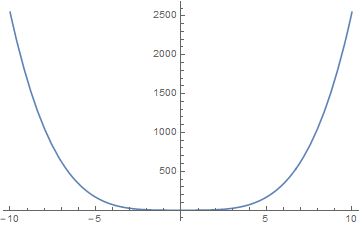
\includegraphics[scale=1]{curve2.png}
	\caption{Plot of potential $V(\phi\cdot \phi)$ with $m^2 > 0$. We notice a unique global minimum.}
\end{figure}

The ground state, or the state of lowest energy, in field theory is called the \textbf{vacuum expectation value}, denoted $\langle \phi \rangle$. In our example the state of lowest energy has zero energy, so
\begin{align}
\langle \phi \rangle  = 0.
\end{align}
Now, we look at whether at $\phi = 0$ there is still symmetry. To do this, we once again use variational methods, i.e., we look at small excitations around the vacuum:
\begin{align}
\phi = \langle \phi \rangle + \epsilon = 0+\epsilon = \epsilon.
\end{align}
In which case, the Lagrangian becomes
\begin{align}
\lag = \frac{1}{2}(\p_\mu\epsilon)(\p^\mu\epsilon) + \frac{1}{2}m^2\epsilon^2+\dots
\end{align}
where the higher order terms are neglected because we're only concerned with infinitesimal variations. Now, by the look of the Lagrangian, we know that the theory is describing a massive particle in real scalar field. So, we have reasons to suspect that excitations in a field gives rise to a particle. We will explore this idea much more deeply as we move on.\\

Now, let us suppose that 
\begin{align}
V(\phi) = -\frac{1}{2}m^2\phi^2 + \frac{1}{4}\lambda \phi^4
\end{align}
then the plot of $V(\phi)$ versus $\phi$ becomes Figure \ref{curve}.\\
\begin{figure}[h!]
	\centering
	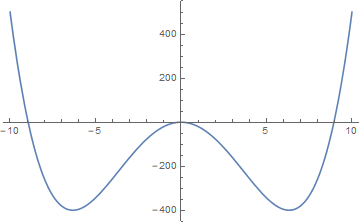
\includegraphics[scale=1]{curve.png}
	\caption{Plot of potential $V(\phi\cdot \phi)$ with $m^2 < 0$. We notice two global minima.}
	\label{curve}
\end{figure}



We observe that there are two possible vacuum solutions. So, we might wonder, well, which one is the vacuum solution? While either one \textit{can} be a solution, nature spontaneously picks one. Let us look at what which $\phi$'s does $V(\phi)$ obtain minimal values:
\begin{align}
\frac{dV}{d\phi} = m^2\phi + \lambda \phi^3 = 0,
\end{align}
i.e.,
\begin{align}
\langle \phi \rangle = \pm \sqrt{\frac{-m^2}{\lambda}}.
\end{align}
Now suppose that nature picks the positive $\phi$:
\begin{align}
\langle \phi \rangle = \sqrt{\frac{-m^2}{\lambda}} \equiv \mathcal{V}.
\end{align}
Now, we can shift to a field defined with respect to the vacuum expectation value:
\begin{align}
\phi' = \phi - \langle \phi \rangle = \phi - \mathcal{V}.
\end{align}
Then 
\begin{align}
\langle \phi' \rangle = 0.
\end{align}
In terms of the Lagrangian, the new Lagrangian is
\begin{align}
\lag = \frac{1}{2}(\p_\mu\phi')(\p^\mu\phi') - (-m^2)\left[ \frac{\phi'^4}{4\mathcal{V}^2} + \frac{\phi'^3}{\mathcal{V}} + \phi'^2 - \frac{\mathcal{V}^2}{4} \right],
\end{align}
which has no symmetry in terms of $\phi'$ (parity transformation). We say that the symmetry is hidden, since we always shift back to get symmetry.\\

Now, we can look at small excitations about $\langle \phi' \rangle$:
\begin{align}
\phi' = \langle \phi' \rangle + \epsilon = 0+\epsilon = \epsilon.
\end{align}
Plugging into the Lagrangian, we get
\begin{align}
\lag = \frac{1}{2}(\p_\mu\epsilon)(\p^\mu\epsilon) - \frac{1}{2}(-2m^2)\epsilon^2,
\end{align}
which acts as a massive particle scalar field with mass (note that we are still assuming $-2m^2 > 0$). Again, we see that by breaking symmetry, we get a massive particle. We shall verify this. Recall the Lagrangian:
\begin{align}
\lag = \frac{1}{2}(\p_\mu\phi)(\p^\mu\phi) - \frac{1}{2}m^2\phi^2 - \frac{1}{4}\lambda \phi^4.
\end{align}
Assume that
\begin{align}
\langle \phi \rangle = \sqrt{\frac{-m^2}{\lambda}} = \mathcal{V}.
\end{align}
Now let
\begin{align}
\phi = \langle \phi \rangle + \epsilon = \mathcal{V} + \epsilon,
\end{align}
where $\mathcal{V}$ is a constant, this gives
\begin{align}
\p_\mu \phi = \p_\mu\epsilon.
\end{align}
Putting everything together, the new $V(\phi)$ is
\begin{align}
V &= \frac{1}{2}m^2(\mathcal{V}+\epsilon)^2 + \frac{1}{4}\lambda(\mathcal{V}+\epsilon)^2 \\
&= \frac{1}{2}m^2(\mathcal{V}^2 + 2\mathcal{V}\epsilon + \epsilon^2) + \frac{1}{4}\lambda(\mathcal{V}^4 + 4\mathcal{V}^3\epsilon + 6\mathcal{V}^2\epsilon^2 + 4\mathcal{V}\epsilon^3 + \epsilon^4).
\end{align}
Keeping the linear terms
\begin{align}
V &\approx \epsilon(m^2 + \mathcal{V}) + \epsilon^2\left( \frac{1}{2}m^2 + \frac{3}{2}\lambda \mathcal{V}^2 \right) + \dots\\
&\approx \epsilon\mathcal{V}(m^2 + \lambda \mathcal{V}^2) + \epsilon^2(-m^2)\\
&\approx \epsilon \mathcal{V}\left( m^2 - \lambda \frac{m^2}{\lambda} \right) + \epsilon^2(-m^2).
\end{align}
So,
\begin{align}
V(\epsilon) \approx -\epsilon^2m^2 = \frac{1}{2}(-2m^2)\epsilon^2.
\end{align}
So the new Lagrangian is verified, as desired. We observe that $V(\epsilon)$ is symmetric around 0.\\

We observe that under a parity transformation, we still get symmetry. We call this \textbf{discrete symmetry}, to distinguish from \textbf{continuous symmetry} under smooth/continuous transformation.\\

\begin{thm}
	\textbf{Goldstone's Theorem:} In a theory with a continuous symmetry that is spontaneously broken, then there will be a massless particle, referred to as \textbf{Nambu-Goldstone mode}. 
\end{thm}
To illustrate the essence of this theorem, we consider two scalar fields written as a vector
\begin{align}
\phi = \begin{pmatrix}
\phi_1 \\ \phi_2
\end{pmatrix},
\end{align}
with an associated Lagrangian defined as
\begin{align}
\lag = \frac{1}{2}(\p_\mu\phi)\cdot(\p^\mu\phi) - V(\phi \cdot \phi).
\end{align}
This theory has a global $O(2)$ symmetry (continuous):
\begin{align}
\phi' = R\phi
\end{align}
where $R$ is just a rotation matrix, by a (continuous) angle $\theta$:
\begin{align}
R = \begin{pmatrix}
\cos\theta & -\sin\theta\\
\sin\theta & \cos\theta
\end{pmatrix}.
\end{align}
Under $R$, the dot product is invariant:
\begin{align}
\phi'^\top\cdot\phi' = (R\phi)^\top(R\phi) = \phi^\top R^\top R\phi = \phi^\top \phi.
\end{align}
So it is clear that the Lagrangian is invariant, as expected:
\begin{align}
\lag' = \lag.
\end{align}
Now, suppose that
\begin{align}
V(\phi\cdot\phi) = \frac{1}{2}m^2\phi\cdot\phi + \frac{1}{4}\lambda(\phi\cdot\phi)^2.
\end{align}
If $m^2 > 0$, then we can plot the potential $V(\phi)$:
\begin{figure}[h!]
	\centering
	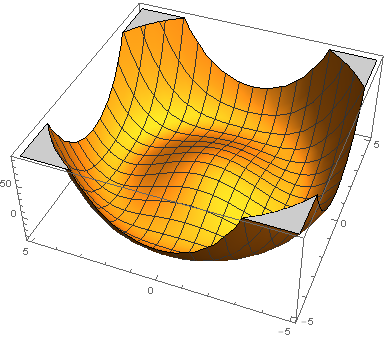
\includegraphics[scale=1]{hat.png}
\end{figure}
Again, we see that there is a unique vacuum solution:
\begin{align}
\langle \phi \rangle = \begin{pmatrix}
0\\0
\end{pmatrix}.
\end{align}
But what if $m^2 < 0$, we get a similar situation at last time, but now in three dimensions where we also have a circle of possible ground state. Now, let nature spontaneously picks a vacuum. We can pick
\begin{align}
\langle \phi \rangle = \begin{pmatrix}
\mathcal{V}\\0
\end{pmatrix}.
\end{align}
Again, let us look at an excitation about $\phi$ and shift:
\begin{align}
\phi' = \phi - \langle \phi \rangle = \begin{pmatrix}
\phi_1\\\phi_2
\end{pmatrix} - \begin{pmatrix}
\mathcal{V}\\0
\end{pmatrix} = 
\begin{pmatrix}
\phi_1 - \mathcal{V}\\\phi_2
\end{pmatrix}.
\end{align}
For small excitations, we can approximate:
\begin{align}
\phi' = \langle \phi'\rangle + \epsilon = \langle \phi' \rangle + \begin{pmatrix}
\eta \\ \xi
\end{pmatrix}=
\begin{pmatrix}
\eta \\ \xi
\end{pmatrix}.
\end{align}
Note that the shift makes $\langle \phi \rangle = 0$.\\

We can express the Lagrangian in terms of these, and find that 
\begin{enumerate}
	\item One field is massless, corresponding to the Nambu-Goldstone mode.
	\item The other is massive, corresponding to the Higgs particle. 
\end{enumerate}


\section{Continuous Global Symmetry}
Consider two scalar fields $\phi_1$ and $\phi_2$, written as
\begin{align}
\phi = \begin{pmatrix}
\phi_1 \\ \phi_2
\end{pmatrix}.
\end{align}
And consider the transformation $\phi' \to R\phi$ where $R$ is a rotation of angle $\theta$ where $\theta$ does not depend on $x$. We can look at the Lagrangian:
\begin{align}
\lag = \frac{1}{2}\p_\mu \phi \cdot \p^\mu \phi - V(\phi \cdot \phi).
\end{align}
For $m^2 < 0$, then 
\begin{align}
V(\phi\cdot \phi) = \frac{1}{2}m^2 \phi^2 + \frac{1}{4}\lambda\phi^2
\end{align}
has minimal value at
\begin{align}
\langle \phi \rangle^2 = \frac{-m^2}{\lambda} \equiv \mathcal{V}^2.
\end{align}
Let's pick 
\begin{align}
\langle \phi \rangle = \begin{pmatrix}
\mathcal{V}\\0
\end{pmatrix}
\end{align}
and do a shift
\begin{align}
\phi' = \phi - \langle \phi \rangle
\end{align}
so that 
\begin{align}
\langle \phi' \rangle = \begin{pmatrix}
0\\0
\end{pmatrix}.
\end{align}
Let us consider excitations around the vacuum:
\begin{align}
\phi' = \langle \phi \rangle + \begin{pmatrix}
\eta \\\zeta
\end{pmatrix} = \begin{pmatrix}
\eta \\ \zeta
\end{pmatrix}
\end{align}
and (again) a shift
\begin{align}
\phi = \langle \phi  \rangle + \phi' = \begin{pmatrix}
\mathcal{V} + \eta \\ \zeta 
\end{pmatrix}
\end{align}
which gives
\begin{align}
\phi \cdot \phi = (\mathcal{V} + \eta )^2 + \zeta^2
\end{align}
and 
\begin{align}
\p_\mu\phi = \p_\mu\phi' = \begin{pmatrix}
\p_\nu\eta\\\p_\mu\zeta
\end{pmatrix}.
\end{align}
We can now write the Lagrangian in terms of the excitations, dropping cubic and higher order terms. First, we find what the new potential looks like:
\begin{align}
V(\phi\cdot\phi) &= \frac{1}{2}m^2\phi^2 + \frac{1}{2}\lambda\phi^4\\
&= \frac{1}{2}m^2\left[ (\mathcal{V} + \eta )^2 + \zeta^2  \right] + \frac{1}{4}\lambda\left[ (\mathcal{V} + \eta )^2 + \zeta^2  \right]^2\\
&= \frac{1}{2}m^2\left[\mathcal{V}^2 + 2\mathcal{V}\eta +\eta^2 + \zeta^2\right] + \frac{1}{4}\lambda\left[\mathcal{V}^2 + 2\mathcal{V}\eta +\eta^2 + \zeta^2\right]^2\\
&= \frac{1}{2}m^2\left[\mathcal{V}^2 + 2\mathcal{V}\eta +\eta^2 + \zeta^2\right] + \frac{1}{4}\lambda\left[4\mathcal{V}^3\eta + 4\mathcal{V}^2\eta^2 + 2\mathcal{V}^2\zeta^2 + 2\mathcal{V}^2\eta^2+\dots\right]\\
&= \eta\left[\frac{1}{2}m^22\mathcal{V} + \frac{1}{4}\lambda4\mathcal{V}^3\right] + \eta^2\left[\frac{1}{2}m^2 + \frac{3}{2}\lambda \mathcal{V}^2\right] + \zeta^2 \left[ \frac{1}{2}m^2 + \frac{\lambda}{2}\mathcal{V}^2+\dots \right] + \dots
\end{align}
Recall that we have defined the minimum:
\begin{align}
\mathcal{V}^2 = -\frac{m^2}{\lambda}.
\end{align}
This gives
\begin{align}
V(\phi^2) &= \mathcal{V}\eta(m^2 + \lambda \mathcal{V}^2) + \eta^2\left[\frac{1}{2}m^2 - \frac{3}{2}m^2\right] + \frac{1}{2}\eta^2(m^2 - m^2).
\end{align}
To second order, this becomes
\begin{align}
V(\phi^2) = -m^2\eta^2 = \frac{1}{2}(-2m^2\eta^2).
\end{align}
So, the Lagrangian is
\begin{align}
\lag &= \frac{1}{2}\p_\mu\phi\p^\mu\phi - V(\phi \cdot \phi)\\
&= \frac{1}{2}\begin{pmatrix}
\p_\mu\eta & \p^\mu\zeta
\end{pmatrix}
\begin{pmatrix}
\p^\mu\eta\\ \p^\mu\zeta
\end{pmatrix} - \left[\frac{1}{2}(-2m^2\eta^2)\right] + \dots\\
&= \frac{1}{2}\left[\p_\mu\eta \p^\mu\eta + \p_\mu\zeta \p^\mu\zeta\right] - \frac{1}{2}(-2m^2)\eta^2+\dots
\end{align}
Notice that we started with two scalars $\phi = \begin{pmatrix}
\phi_1&\phi_2
\end{pmatrix}^\top$ and the wrong sign $m^2 < 0$. But after spontaneous symmetry breaking and a physical vacuum excitation, we have
\begin{align}
\lag = \boxed{\frac{1}{2}\p_\mu\eta \p^\mu\eta - \frac{1}{2}(-2m^2)\eta^2} + \boxed{\frac{1}{2}\p_\mu\zeta \p^\mu\zeta}
\end{align}
Observe that we a get 1 massive scalar field $\eta$ with mass $-2m^2 > 0$ and a massless scalar $\zeta$. The massive scalar field is what we will ultimately describe as the \textbf{Higgs boson}, while the massless field describes the Nambu-Goldstone mode. Let us revisit the Goldstone theorem:\\

\begin{thm}
	\textbf{Goldstone:} For every continuous global symmetry that is spontaneously broken, there emerges a massless particle. 
\end{thm}

For example, in electromagnetism, there is a U(1) local gauge symmetry. We have shown earlier that this gives rise to the massless photon.\\

There are slight ``exceptions'' to the rule, though. Some issues might arise when we try to describe the weak interaction. We would like to describe the force-carrying particles in the weak interactions as a gauge theory. SU(2) gives us 3 gauge fields. However, since the weak interaction is too weak and short-ranged, it was suspected that the weak force is carried by 3 massive vector fields. But, the problem is that, according to Goldstone's theorem, we can't have both a gauge symmetry and massive terms for the gauge fields. \\

\begin{rmk}
	Any interacting massless particle is detectable because it's got a long-range interaction. This implies that particles in Nambu-Goldstone modes are detectable. 
\end{rmk}

\section{An O(2) example}
So far, we have looked at spontaneous symmetry breaking of of a global gauge theory. Now, we will look at spontaneous symmetry breaking of a local gauge theory. This subsection is essentially about Higgs and others found a mechanism where the massless Nambu-Goldstone modes get ``eaten'' and the gauge fields acquire mass. \\

Consider a local O(2) transformation and consider (once again) 2 real scalar fields $\phi_1, \phi_2$, written as a vector.
\begin{align}
\phi = \begin{pmatrix}
\phi_1 \\ \phi_2
\end{pmatrix}.
\end{align}
The transformation is essentially a rotation, we shall call $R$. For the sake of simplicity, we can take $R$ as a 2$\times$2 matrix. So, the transformation has the form:
\begin{align}
\phi' = R(x)\phi = \begin{pmatrix}
\cos\alpha(x)&-\sin\alpha(x)\\\sin\alpha(x)&\cos\alpha(x)
\end{pmatrix}\begin{pmatrix}
\phi_1 \\ \phi_2
\end{pmatrix},
\end{align}
where the angle of rotation $\alpha$ depends on the coordinates (hence local). Also note that since the determinant of $R$ is 1, this transformation can also be classified as a special orthogonal transformation, belonging to SO(2), an abelian group.\\

To greatly simplify our notation, we can write the transformation $\phi \to \phi'$ as
\begin{align}
R = e^{i\alpha(x)T}
\end{align}
where $T$ is a $2\times 2$ generator. For this particular transformation, $T$ is Hermitian 
\begin{align}
T = \begin{pmatrix}
0 & i\\
-i & 0
\end{pmatrix}.
\end{align}
It might be useful later to observe that
\begin{align}
T^2 = T\\T^\top = -T \\ T^{\dagger} = T.
\end{align}
For small $\alpha(x)$, the transformation reduces into a much simpler form:
\begin{align}
R &\approx I + i\alpha(x)T\\
&= \begin{pmatrix}
1&0\\0&1
\end{pmatrix} + i\alpha(x)\begin{pmatrix}
0 & i\\-i&0
\end{pmatrix} = 
\begin{pmatrix}
1 -\alpha\\\alpha 1
\end{pmatrix}.
\end{align}
Let us return to our original Lagrangian:
\begin{align}
\lag = \frac{1}{2}\p_\mu\phi \cdot \p^\mu\phi - V(\phi\cdot \phi).
\end{align}
Let $\phi \to \phi' = R(x)\phi$, we get 
\begin{align}
\p_\mu\phi = \p_\mu\phi' = R\p_\mu\phi + (\p_\mu R)\phi.
\end{align}
Notice that there is no local symmetry here, which means we ought to fix this by changing the derivative (as before), i.e., we need to define a gauge-covariant derivative:
\begin{align}
D_\mu = \p_\mu + igA_\mu
\end{align}
where $g$ is a coupling constant and $A_\mu ~ TA_\mu$ is some (matrix) function (note that we are still working with matrices here). Formally, in order for $D_\mu$ to act on $\phi$, it has to be a 2$\times $2 matrix. So formally,
\begin{align}
\boxed{D_\mu = I\p_\mu + TigA_\mu}
\end{align} 
where $I$ is the identity matrix, and $T$ is the generator. Now, to obtain gauge invariance, we want $D_\mu\phi \to D'_\mu\phi' = RD_\mu\phi$ so that
\begin{align}
D_\mu\phi \cdot D^\mu\phi \to \left(RD_\mu\phi\right)^\top \left(RD^\mu\phi\right) &=  (D_\mu\phi)^\top R^\top R (D^\mu\phi)\\
&= (D_\mu\phi)^\top(D^\mu\phi)\\
&= (D_\mu\phi)\cdot(D^\mu\phi).
\end{align}
The question is: how must $A_\mu$ transform in order for this to hold? Recall what we have done in the previous sections when we required that $A_\mu$ transforms as
\begin{align}
A'_\mu = A_\mu + \p_\mu\Lambda
\end{align}
in order to get gauge invariance in electromagnetism. To find how $A_\mu$ has to transform here, we follow sort of a similar path, while keeping in mind that $A_\mu$ is actually a matrix. To do this, we first look at
\begin{align}
D'_\mu\phi' &= (\p_\mu + iqA'_\mu)R\phi\\
&= R\p_\mu\phi + (\p_\mu R)\phi + iqA'_\mu R\phi.
\end{align}
Since we require invariance, we set
\begin{align}
D'_\mu\phi' = RD_\mu\phi,
\end{align}
i.e., we set
\begin{align}
R\p_\mu\phi + (\p_\mu R)\phi + iqA'_\mu R\phi &= R(\p_\mu iqA_\mu)\phi 
\end{align}
which says
\begin{align}
R\p_\mu\phi + (\p_\mu R)\phi + iqA'_\mu R\phi &= R\p_\mu\phi  RiqA_\mu\phi,
\end{align}
which is satisfied if
\begin{align}
igA'_\mu R\phi = igRA_\mu - (\p_\mu R)\phi.
\end{align}
So,
\begin{align}
\frac{ig}{ig}A'_\mu R &= RA_\mu - \frac{1}{ig}\p_\mu R\\
A'_\mu RR^{-1} &= RA_\mu R^{-1} + \frac{i}{g}(\p_\mu R)R^{-1}.
\end{align}
But since $R^{-1}R = RR^{-1} = 1$,
\begin{align}
\boxed{A'_\mu = RA_\mu R^{-1} + \frac{i}{g}(\p_\mu R)R^{-1}}
\end{align}
This is the transformation rule for $A_\mu$ under a local O(2) gauge transformation.\\

Let us consider a quick educated example. With
\begin{align}
R &= e^{i\alpha(x)T}\\
R^{-1} &= e^{-i\alpha(x)T},
\end{align}
we get
\begin{align}
A_\mu \to A'_\mu &= RA_\mu R^{-1} + \frac{i}{g}(\p_\mu R)R^{-1}\\
&= e^{i\alpha(x)T}A_\mu e^{-i\alpha(x)T} + \frac{i}{g}\left(i(\p_\mu\alpha)TR\right)R^{-1}.
\end{align}
Recall that $A_\mu$ is a matrix. So, actually $A_\mu$ is written as
\begin{align}
A_\mu \equiv A_\mu T.
\end{align}
So, we actually have
\begin{align}
A'_\mu T = A_\mu T e^{i\alpha(x)T}e^{-i\alpha(x)T} - \frac{1}{g}(\p_\mu\alpha(x))T.
\end{align}
So, the function $A_\mu$ must obey
\begin{align}
A'_\mu = A_\mu - \frac{1}{g}(\p_\mu\alpha).
\end{align}
Looks familiar? You're right, because we have seen this before in studying the Maxwell's equations. If we define
\begin{align}
\Lambda(x) = - \frac{\alpha(x)}{g}
\end{align}
then we get the familiar transformation rule for $A_\mu$:
\begin{align}
A'_\mu = A_\mu + \p_\mu \lambda(x).
\end{align}
Note that, as a bonus we also get
\begin{align}
F_{\mu\nu} = \p_\mu A_\nu - \p_\nu A_\mu,
\end{align}
which implies an anti-symmetry in the electromagnetic field strength tensor
\begin{align}
F_{\mu\nu} = -F_{\nu\mu},
\end{align}
which carries a gauge invariance. Now that we know the transformation rule for $A_\mu$ and have defined $F_{\mu\nu}$ in such a way that it is gauge invariant, we can add it to the Lagrangian to make the theory (local O(2) gauge theory, that is) dynamical. The complete Lagrangian for this theory is then
\begin{align}
\lag = \frac{1}{2}(D_\mu\phi)\cdot(D^\mu\phi) - V(\phi\cdot\phi) - \frac{1}{4}F^{\mu\nu}F_{\mu\nu}.
\end{align}


But note that this is only true for the simple case of a $O(2)$ transformation. To find how $A_\mu$ transforms in general, we have to use the general, boxed equation that involves $R$ and $R^{-1}$. 


\section{Introduction to the Higgs Mechanism}
To summarize what we have been doing so far, consider (once again) the potential
\begin{align}
V(\phi\cdot\phi) = \frac{1}{2}m^2\phi^2 + \frac{1}{4}\lambda(\phi\cdot\phi)^2.
\end{align}
If $m^2 > 0$, then there is spontaneous symmetry breaking, i.e. we get massless $A_\mu$ with 2 modes of motion (we have shown this in the worked problems) and 2 massive scalar fields $\phi_1$ and $\phi_2$, i.e., two Nambu-Goldston modes and two massive modes.\\

On the other hand, if $m^2 < 0$, we get spontaneous symmetry breaking, and Goldstone theorem says that for a global symmetry, we get one massive Higgs scalar and one massless Nambu-Goldstone mode, totaling two rather than 4. (Note that this is not true for local symmetry)\\

Motivated by our recent example, now we will show how spontaneous symmetry breaking in O(2) can give rise to the Higgs mechanism. We will show that in this symmetry breaking process, the Nambu-Goldstone mode gets ``eaten'' (this is actually a technical term) and $A_\mu \to A'_\mu$, which is massive. Ultimately, we will show that we are left with a massive $A'_\mu$ with three modes and a massive Higgs scalar without any Nambu-Goldstone modes, totaling (once again) 4 modes.  \\

Recall the Lagrangian of the form
\begin{align}
\lag = \frac{1}{2}(D_\mu\phi)\cdot(D^\mu\phi) - V(\phi\cdot\phi) - \frac{1}{4}F^{\mu\nu}F_{\mu\nu}.
\end{align}
with 
\begin{align}
\phi = \begin{pmatrix}
\phi_1\\\phi_2
\end{pmatrix}
\end{align}
and
\begin{align}
D_\mu\phi = (\p_\mu \mathbb{I} - igTA_\mu).
\end{align}
We recall that this has an O(2) invariance with
\begin{align}
\begin{cases}
&\phi \to \phi' = R\phi\\
&A_\mu\to A\_\mu = RA_\mu R^{-1} + \frac{i}{g}(\p_\mu R)R^{-1}.
\end{cases}
\end{align}
To see how the Higgs mechanism comes about, we shall consider an illustrating example in O(2) with a re-parameterization of $\phi$. We shall write 
\begin{align}
\phi = R^{-1}\phi = R^{-1}\begin{pmatrix}
0\\\mathcal{V} + \mathcal{E}
\end{pmatrix}
\end{align}
and let
\begin{align}
\alpha = \frac{\zeta}{\mathcal{V}},
\end{align}
where these terms are defined in the previous subsection. With this, we get
\begin{align}
R^{-1} = e^{-i\alpha T} \approx \begin{pmatrix}
1 & \alpha \\
-\alpha & 1
\end{pmatrix}
=
\begin{pmatrix}
1 & \zeta/\mathcal{V}\\
-\zeta/\mathcal{V} & 1
\end{pmatrix}.
\end{align}
This gives us a new expression for $\phi$:
\begin{align}
\phi = R^{-1}\phi' = \begin{pmatrix}
1 & \zeta/\mathcal{V}\\
-\zeta/\mathcal{V} & 1
\end{pmatrix}\begin{pmatrix}
0\\\mathcal{V} + \mathcal{E}
\end{pmatrix} \approx \begin{pmatrix}
\zeta \\ \mathcal{V} + \mathcal{E}
\end{pmatrix}.
\end{align}
This is in fact the expression we obtained earlier in the previous subsection, where $\mathcal{E}$ denotes a small excitation. This re-parameterization is called the ``Unitary Gauge.''\\

Now, let us put this new $\phi$ into the Lagrangian:
\begin{align}
\lag = \frac{1}{2}D_\mu (R^{-1}\phi')\cdot D^{\mu}(R^{-1}\phi') - V(R^{-1}\phi' \cdot R^{-1}\phi') - \frac{1}{4}F_{\mu\nu}F^{\mu\nu}.
\end{align} 
Since this is gauge invariant, we can perform a gauge transformation:
\begin{align}
\begin{cases}
&\phi \to R\phi = R\circ R^{-1}\phi' = \phi'\\
&A_\mu \to A'_\mu,
\end{cases}
\end{align}
which gives
\begin{align}
\lag = \frac{1}{2}D'_\mu \phi' \cdot D^{'\mu}\phi' - V(\phi'\cdot \phi')- \frac{1}{4}F'_{\mu\nu}F^{'\mu\nu}.
\end{align}
Now, we note that 
\begin{align}
\phi'\cdot\phi' = (\mathcal{V} + \mathcal{E})^2,
\end{align}
so, keeping only the quadratic terms
\begin{align}
V(\phi'\cdot \phi') &= \frac{1}{2}m^2(\mathcal{V} + \mathcal{E})^2 + \frac{1}{4}\lambda (\mathcal{V} + \mathcal{E})^4\\
&=\mathcal{E}(m^2\mathcal{V} + \lambda \mathcal{V}^3) + \mathcal{E}^2\left(\frac{1}{2}m^2 + \frac{3}{2}\lambda \mathcal{V}^2 + \dots\right).
\end{align}
But because
\begin{align}
\mathcal{V}^2 = \frac{-m^2}{\lambda},
\end{align}
$V(\phi'\cdot \phi')$ simplifies to
\begin{align}
V(\phi' \cdot \phi') &\approx \mathcal{E}(-\lambda \mathcal{V}^3 + \lambda \mathcal{V}^3) + \mathcal{E}^2\left(\frac{1}{2}m^2 - \frac{3}{2}m^2 + \dots\right)\\
&\approx -\mathcal{E}^2m^2\\
&= \frac{1}{2}(-2m^2)\mathcal{E}^2.
\end{align}
We also need to look at how $D_\mu$ changes:
\begin{align}
D'_\mu &= (\mathbb{I}\p_\mu + ig TA'_\mu)\\
&= \begin{pmatrix}
\p_\mu & 0 \\
0& \p_\mu
\end{pmatrix} +
ig\begin{pmatrix}
0 & i \\
-i & 0
\end{pmatrix}A'_\mu\\
&= \begin{pmatrix}
\p_\mu & -igA'_\mu\\
igA'_\mu &  \p_\mu
\end{pmatrix}.
\end{align}
So,
\begin{align}
D'_\mu \phi' &= \begin{pmatrix}
\p_\mu & -igA'_\mu\\
igA'_\mu &  \p_\mu
\end{pmatrix}\begin{pmatrix}
0 \\ \mathcal{V} + \mathcal{E} \end{pmatrix}\\ &= \begin{pmatrix}
-gA'_\mu (\mathcal{V} + \mathcal{E})\\
\p_\mu \mathcal{E}
\end{pmatrix}.
\end{align}
Therefore,
\begin{align}
D'_\mu \phi' \cdot D^{'\mu}\phi' &= \begin{pmatrix}
-gA'_\mu (\mathcal{V} + \mathcal{E})\\
\p_\mu \mathcal{E}
\end{pmatrix}^\top\begin{pmatrix}
-gA^{'\mu} (\mathcal{V} + \mathcal{E})\\
\p^\mu \mathcal{E}
\end{pmatrix}\\
 &= g^2 A'_\mu A^{'\mu}(\mathcal{V} + \mathcal{E})^2 + \p_\mu \mathcal{E} \p^\mu \mathcal{E}.
\end{align}
Thus the Lagrangian becomes:
\begin{align}
\lag &= \frac{1}{2}\p_\mu\E\p^\mu\E - \frac{1}{2}(-2m^2)\mathcal{E}^2 - \frac{1}{4}F'_{\mu\nu}F^{'\mu\nu}\\ 
&\hspace{0.5cm}+ \frac{g^2\mathcal{V}^2}{2}A'_\mu A^{'\mu} + \frac{g^2}{2}(2\mathcal{E}\mathcal{V} + \mathcal{E}^2)A'_\mu A^{'\mu} + \dots 
\end{align}
What does this theory describe? We shall break this down term-by-term:
\begin{enumerate}
	\item The two terms:
	\begin{align}
	\frac{1}{2}\p_\mu\E\p^\mu\E - \frac{1}{2}(-2m^2)\mathcal{E}^2
	\end{align}
	which has $-m^2 > 0$ describe a massive scalar, spin 0 particle. This particle is called \textbf{the Higgs boson}. \\
	
	\item The next two terms:
	\begin{align}
	- \frac{1}{4}F'_{\mu\nu}F^{'\mu\nu} + \frac{g^2\mathcal{V}^2}{2}A'_\mu A^{'\mu}
	\end{align}
	describe a massive vector gauge field (recall what we have derived in the electromagnetism section)\\
	
	\item And the last (significant) term:
	\begin{align}
	\frac{g^2}{2}(2\mathcal{E}\mathcal{V} + \mathcal{E}^2)A'_\mu A^{'\mu}
	\end{align}
	is the interaction between $\mathcal{E}$ and $A'_\mu$.
\end{enumerate}

Now, notice that we do not have a massless Nambu-Goldstone mode (the $\zeta$ term is long gone). We say that this mode has got ``eaten'', resulting in $A_\mu$ becoming a massive $A'_\mu$. We can also count the degrees of freedom again to see what have changed. Recall that before spontaneous symmetry breaking, we have 2 modes for the massless vector field $A_\mu$ (the photon) and 2 massive modes for $\phi = \begin{pmatrix}
\phi_1 & \phi_2
\end{pmatrix}^\top$. So we had 4 in total. After spontaneous symmetry breaking, we have 1 degree of freedom for the massive scalar field $\mathcal{E}$, and 3 for the massive gauge field $A'_\mu$ (we will show why there are 3 degrees of freedom in the Worked Problems section). So, we also end up with 4 degrees of freedom, except without a massless mode. \\

Note that since O(2) is U(1) are very similar, we will not work out the details of spontaneous symmetry breaking of U(1) gauge theory here. This will serve as an exercise that will be covered in its entirety (theory derived from scratch) in the Worked Problems section. \\




































\newpage

\chapter{Gravitation and Lagrangian Formulation of General Relativity}

\section{Review of General Relativity \& Curved Spacetime}

\subsection{General Relativity}

Taking the speed of light, $c$, to be 1, the Einstein equation for general relativity is
\begin{align}
R_{\mu\nu} - \frac{1}{2}Rg_{\mu\nu} = 8\pi GT_{\mu\nu}.
\end{align}
Sometimes, it is more useful to write the Einstein's equation as
\begin{align}
R_{\mu\nu} = 8\pi G \left( T_{\mu\nu} - \frac{1}{2}Tg_{\mu\nu} \right).
\end{align}
In vacuum, where all components of the energy-momentum stress tensor are zero, the Einstein's equation becomes
\begin{align}
R_{\mu\nu} = 0.
\end{align}

\subsection{Curved Spacetime}
Perhaps the most important change as we go from flat to general curved spacetime is the notion of the ``derivative.'' In introduction to general relativity, we have introduced the \textbf{covariant derivative} and \textbf{absolute derivative}. We shall revisit the covariant derivative, as it will be important in the derivation of Lagrangian formulation of gravitation. The covariant derivative has the form - or forms, should I say:
\begin{align}
D_\mu w_\nu &= \p_\mu w_\nu - \Gamma^\lambda_{\mu\nu}w_\lambda\\
D_\mu v^\nu &= \p_\mu v^\nu + \Gamma^\nu_{\lambda\nu}v^\lambda.
\end{align}
Note the sign difference in the definitions. The covariant derivative is defined \textit{differently} for covariant and contravariant vectors. In fact, this follows if we define the covariant derivative for one kind of vectors.
\begin{propty}
	Strictly speaking, some of theses properties are required for the definition of the covariant derivative to make sense and work. 
	\begin{enumerate}
		\item Linearity: $D(U+V) = D(U) + D(V)$
		\item Product rule: $D(U\otimes V) = D(U)\otimes D(V)$
		\item Commutes with contractions: $D_\mu(\tensor{T}{^{\lambda}_{\lambda\rho}}) = \tensor{(DT)}{_\mu^\lambda_{\lambda\rho}}$
	\end{enumerate}
\end{propty} 
Next, recall the definition of the \textbf{Christoffel symbol}:
\begin{align}
\Gamma^{\lambda}_{\mu\nu} = \frac{1}{2}g^{\lambda\rho}\left(
   \p_{\mu}g_{\rho\nu}
 + \p_{\nu}g_{\mu\rho}
 - \p_{\rho}g_{\mu\nu}
 \right).
\end{align}
Now, consider a contravariant vector $V^\mu$, we can define the \textbf{divergence} in curved spacetime based on the flat 3-space definition
\begin{align}
\text{div}\vec{V} = \p_i V^i
\end{align}
by ``contracting'' an index and adding the Christoffel symbols:
\begin{align}
D_\mu V^\mu = \p_\mu V^\mu + \Gamma^\mu_{\mu\lambda}V^\lambda.
\end{align}
Next, invoking the definition of the Christoffel symbols, we can compute 
\begin{align}
\Gamma^\mu_{\mu\lambda} &= \frac{1}{2}g^{\mu\rho}(\p_\mu g_{\rho\lambda} + \p_\lambda g_{\rho\mu} - \p_\rho g_{\mu\lambda})\\
&= a
\end{align}

\section{Lagrangian Formulation}

\section{Overview}



The action is
\begin{align}
S = \int \lag (\Phi^i, D_\mu \Phi^i)\,d^nx.
\end{align}
$\lag$ is a density. 
\begin{align}
\lag = \sqrt{-g}\hat{\lag}
\end{align}
where $\hat{\lag}$ is a scalar and
\begin{align}
g = \det(g_{ij})
\end{align}
is the determinant of the metric tensor. The associated Euler-Lagrange equation is
\begin{align}
\frac{\p \hat{\lag}}{\p \Phi} - D_\mu \left( \frac{\p \hat{\lag}}{\p (D_\mu \Phi)}\right) = 0.
\end{align}
Recall Stokes' theorem:
\begin{align}
\int_\Sigma \nabla_\mu V^\mu \sqrt{\vert g\vert}\,d^nx = \int_{\p\Sigma} n_\mu V^\mu \sqrt{\vert \gamma \vert},d^{n-1}x.
\end{align}
Setting the variation equal to zero at the boundary and integrate by parts give
\begin{align}
\int A^\mu (D_\mu B)\sqrt{-g}\,d^nx = -\int (D_\mu A^\mu)B\sqrt{-g}\,d^n x + \text{ boundary terms}.
\end{align}
\begin{align}
S_\phi = \int \left[ -\frac{1}{2}g^{\mu\nu}(D_\mu \phi)(D_\nu\phi) - V(\phi) \right]\sqrt{-g}\,d^nx,
\end{align}
The equation of motion:
\begin{align}
\square \phi - \frac{dV}{d\phi} = 0.
\end{align}
The \textbf{covariant d'Alembertian} now becomes
\begin{align}
\square \equiv D^\mu D_\mu \equiv g^{\mu\nu}D_\mu D_\nu.
\end{align}
\textbf{The Hilbert action}
\begin{align}
S_H = \int \sqrt{-g}\,d^nx.
\end{align}



\subsection{Introduction to the Lagrangian Formulation of General Relativity}

Recall that the action in flat spacetime has the form:
\begin{align}
S = \int \lag \,d^4x.
\end{align}

This is due to the fact that the metric is just $\eta_{\mu\nu} = \text{diag}(1,-1,-1,-1)$. But in curved spacetime, however, the metric is $g_{\mu\nu} \neq \eta_{\mu\nu}$. In some sense we can find how the form of the action changes as we move from flat to general curved spacetime. Consider the transformation $x^\mu \to x^{\mu'}$, then $dx^\mu \to X^{\mu'}_\nu dx^\nu$. The Jacobian matrix for this transformation is 
\begin{align}
\lb X^{\mu'}_\nu \rb = \lb\f{\p x^{\mu'}}{\p x^\nu}\rb
\end{align} 
and
\begin{align}
g_{\mu'\nu'} = X^\alpha_{\mu'}X^\beta_{\nu'}g_{\alpha\beta}.
\end{align}
So the ``volume'' element becomes:
\begin{align}
d^4x \to  d^4x' = \bigg\vert \f{\p x^{\mu'}}{\p x^\nu}  \bigg\vert d^4x.
\end{align}
Since we want our volume element to be invariant, we have to compensate with a factor of 
\begin{align}\label{det}
g = \det(g_{\mu\nu}) = \vert g_{\mu\nu} \vert.
\end{align}
But we are not quite there yet. Notice that the metric tensor has the form
\begin{align}
[g_{\mu\nu}] = \begin{pmatrix}
+ &&&\\
&-&&\\
&&-&\\
&&&-
\end{pmatrix},
\end{align}
which means $\det(g_{\mu\nu}) < 0$. So, we use $-g > 0$. From Eq. \eqref{det}, we get that 
\begin{align}
g' = \bigg\vert \f{\p x}{\p x'} \bigg\vert^2 g.
\end{align}
So,
\begin{align}
g' = \bigg\vert \f{\p x'}{\p x} \bigg\vert^{-2} g,
\end{align}
which means
\begin{align}
\sqrt{-g'} = \bigg\vert \f{\p x'}{\p x} \bigg\vert^{-1}\sqrt{-g},
\end{align}
since $-g, -g' > 0$. Therefore,
\begin{align}
d^4 x \sqrt{-g} = d^4 x' \bigg\vert \f{\p x'}{\p x} \bigg\vert^{-1} \bigg\vert \f{\p x'}{\p x} \bigg\vert \sqrt{-g'} = d^4 x' \sqrt{-g'}.
\end{align} 
We have 
\begin{align}
d^4x\sqrt{-g} = d^4x' \sqrt{-g'}
\end{align}
as desired. Now, just for sanity check, we can return to flat spacetime where $g'_{\mu\nu} = g_{\mu\nu} = \eta_{\mu\nu} = \text{diag}(1,-1,-1,-1)$. Then, $-g = 1$ hence $\sqrt{-g} = 1$, which says $d^4x \sqrt{-g} = d^4x = d^4x' = d^4x'\sqrt{-g'}$. So, for curved spaces the action is given by
\begin{align}
\boxed{S = \int \,d^4x \sqrt{-g}\lag}
\end{align}


For pure gravity (no matter), the action is called the \textbf{Einstein-Hilbert action}
\begin{align}
\boxed{S = \int \, d^4x \sqrt{-g}\f{1}{16\pi G}R}
\end{align}
where $R$ is the \textbf{Ricci scalar}, defined by a contraction
\begin{align}
R = \tensor{R}{^\mu_\mu} = \tensor{R}{^{\mu\nu}_{\mu\nu}} = g^{\mu\nu} R_{\mu\nu} 
\end{align}
where $R_{\mu\nu}$ is defined in terms of other contractions
\begin{align}
R_{\mu\nu} = \tensor{R}{^\lambda_{\mu\lambda\nu}} = g^{\lambda \rho} R_{\rho\mu\lambda\nu}.
\end{align}
We also recall that
\begin{align}
\tensor{R}{^\rho_{\sigma\mu\nu}} = \p_\mu \Gamma^\rho_{\nu\sigma} - \p_\nu \Gamma^\rho_{\mu\sigma} + \Gamma^\rho _{\mu\lambda}\Gamma^\lambda_{\nu\sigma} - \Gamma^\rho_{\nu\lambda} \Gamma^\lambda_{\mu\sigma}
\end{align}
where the \textbf{Christoffel symbols} are defined in terms of the metric tensor:
\begin{align}
\Gamma^\lambda_{\mu\nu} = \f{1}{2}g^{\lambda\sigma}\lp \p_\mu g_{\nu\sigma} + \p_\nu g_{\sigma\mu} - \p_\sigma g_{\mu\nu} \rp.
\end{align}










\subsection{Variation on the metric tensor, without matter: $T_{\mu\nu} = 0$}

To find the physical laws or the equations of motion, we need to vary the action with respect to $g_{\mu\nu}$ and $g^{\mu\nu}$ since it is written in terms of the metric (the field of interest is the metric). To start, we must pick $g_{\mu\nu}$ or $g^{\mu\nu}$ as the fundamental field. The choice shouldn't matter, but for certain conveniences, we shall pick $g^{\mu\nu}$ as the fundamental field. 

Now, $g_{\mu\nu}$ (the metric tensor) and $g^{\mu\nu}$ (its inverse) obey
\begin{align}
g^{\mu\nu}g_{\nu\sigma} = \delta^\nu_\sigma,
\end{align}  
which is covariantly constant. So,
\begin{align}
(\delta g^{\mu\nu}) g_{\nu\sigma} + g^{\mu\nu}(\delta g_{\nu\sigma}) = 0,
\end{align}
i.e.,
\begin{align}
(\delta g^{\mu\nu}) g_{\nu\sigma} = -g^{\mu\nu}(\delta g_{\nu\sigma})
\end{align}
Multiplying with $g^{\sigma\rho}$ we get
\begin{align}
(\delta g^{\mu\nu})g_{\nu\sigma}g^{\sigma\rho} &= -g^{\mu\nu}g^{\sigma\rho}(\delta g_{\nu\sigma})\\
(\delta g^{\mu\nu})\delta^\nu_\rho &=  -g^{\mu\nu}g^{\sigma\rho}(\delta g_{\nu\sigma})
\end{align}
i.e.,
\begin{align}
\delta g^{\mu\rho} = -g^{\mu\nu}g^{\sigma\rho}\delta g_{\nu\sigma}.
\end{align}
We an rewrite this as
\begin{align}
\delta g^{\mu\nu} = -g^{\mu\alpha} g^{\nu\beta}\delta g_{\alpha\beta}.
\end{align}
Likewise, 
\begin{align}
\delta g_{\mu\nu} = -g_{\mu\alpha}g_{\nu\beta}\delta g^{\alpha\beta}.
\end{align}

Now, consider 
\begin{align}
\sqrt{-g}\lag \sim \sqrt{-g}R = \sqrt{-g}g^{\mu\nu}R_{\mu\nu}
\end{align}
We have,
\begin{align}
\delta(\sqrt{-g}\lag) &\sim \delta (\sqrt{-g} R)\nn\\
&=\delta\lb \sqrt{-g}g^{\mu\nu}R_{\mu\nu} \rb\nn\\
&= (\delta \sqrt{-g})g^{\mu\nu}R_{\mu\nu} + \sqrt{-g}(\delta g^{\mu\nu})R_{\mu\nu} + (\sqrt{-g})g^{\mu\nu}(\delta R_{\mu\nu}).  
\end{align}

First, we want to find $\delta \sqrt{-g}$ in terms of $\delta g^{\mu\nu}$. We already know that $g = \det(g_{\mu\nu})$, so we use the following identity for matrices
\begin{align}
\ln(\det(M)) = \Tr(\ln(M)),
\end{align}
which can be a fun exercise to verify. Varying this identity, we get
\begin{align}
\delta \ln(\det(M)) = \delta \Tr(\ln(M)),
\end{align}
i.e.,
\begin{align}
\f{1}{\det(M)}\delta \det(M) = \Tr(\delta \ln(M)) = \Tr(M^{-1}\delta M).
\end{align}
If we let $M = [g_{\mu\nu}]$ and $M^{-1} = [g^{\mu\nu}]$ then we have
\begin{align}
\ln(g) = \Tr(\ln[g_{\mu\nu}]).
\end{align}
Varying with respect to the metric, we get
\begin{align}
\f{1}{g}(\delta g) = \Tr(g^{\mu\nu}\delta g_{\mu\nu}).
\end{align}
But since $g^{\mu\nu}\delta g_{\mu\nu}$ is just a number, $\Tr(g^{\mu\nu}\delta g_{\mu\nu}) = g^{\mu\nu}\delta g_{\mu\nu}$. Hence,
\begin{align}
\boxed{\delta g = g g^{\mu\nu}\delta g_{\mu\nu} = -gg_{\mu\nu}\delta g^{\mu\nu}}.
\end{align}
Then
\begin{align}
\delta \sqrt{-g} &= \delta (-g)^{1/2\nn}\\
& = \f{1}{2}(-g)^{-1/2}\delta (-g) \nn\\
&= \f{-1}{2}\f{1}{\sqrt{-g}}\delta g \nn\\
&= \f{-1}{2}\f{1}{\sqrt{-g}}(-g)g_{\mu\nu}\delta g^{\mu\nu}\nn\\
&= \f{-1}{2}\sqrt{-g}g_{\mu\nu} \delta g^{\mu\nu}
\end{align}
i.e.,
\begin{align}
\boxed{\delta \sqrt{-g} = \f{-1}{2}\sqrt{-g}g_{\mu\nu} \delta g^{\mu\nu} = \f{1}{2}\sqrt{-g}g^{\mu\nu}\delta g_{\mu\nu}}
\end{align}
Now, what about $\delta R = \delta R_{\mu\nu}$? Recall that
\begin{align}
\delta (\sqrt{-g} R) &= (\delta \sqrt{-g})(g^{\mu\nu}R_{\mu\nu}) + \sqrt{-g}(\delta g^{\mu\nu})R_{\mu\nu} + (\sqrt{-g})g^{\mu\nu}(\delta R_{\mu\nu})\nn\\
&= (\delta \sqrt{-g})R + \sqrt{-g}(\delta g^{\mu\nu})R_{\mu\nu} + (\sqrt{-g})g^{\mu\nu}(\delta R_{\mu\nu})\nn\\
&= \f{-1}{2}\sqrt{-g}g_{\mu\nu}( \delta g^{\mu\nu})R + \sqrt{-g}(\delta g^{\mu\nu})R_{\mu\nu} + (\sqrt{-g})g^{\mu\nu}(\delta R_{\mu\nu})
\end{align} 
Since we have found $\delta \sqrt{-g}$ in terms of $\delta g^{\mu\nu}$, 
\begin{align}
\delta (\sqrt{-g}R ) = \sqrt{-g}\lp R_{\mu\nu} - \f{1}{2}g_{\mu\nu}R \rp\delta g^{\mu\nu} + \sqrt{-g}g^{\mu\nu}\delta R_{\mu\nu}.
\end{align}
We immediately recognize the Einstein tensor $G_{\mu\nu}$ 
\begin{align}
G_{\mu\nu} = R_{\mu\nu} - \f{1}{2}g_{\mu\nu}R.
\end{align}
From the Einstein equations, we know that 
\begin{align}
G_{\mu\nu} = 8\pi G T_{\mu\nu}.
\end{align}
But since there is no matter, $T_{\mu\nu} = 0$, i.e., $G_{\mu\nu} = 0$. So, if we do the variations correctly, we should get
\begin{align}
R_{\mu\nu} - \f{1}{2}g_{\mu\nu}R = 0.
\end{align}

It turns out that after some simplification
\begin{align}\label{R}
\boxed{\int \,d^4x \sqrt{-g}g^{\mu\nu}\delta R_{\mu\nu} = 0}
\end{align}
which means we don't have to worry about the third term in the expansion of $\delta \sqrt{-g}R$ that involves $\delta R_{\mu\nu}$. Therefore, with
\begin{align}
S = \int \,d^4x \sqrt{-g}\f{1}{16\pi G}R,
\end{align}
we have
\begin{align}
16\pi G \delta S = \int\,d^4x \sqrt{-g}\lp R_{\mu\nu} - \f{1}{2}g_{\mu\nu}R \rp\delta g^{\mu\nu} = 0,
\end{align}
since we require varying the action gives zero, which implies 
\begin{align}
\boxed{R_{\mu\nu} - \f{1}{2}g_{\mu\nu}R = 0}
\end{align}
as expected.\\


















\begin{exmp}
	Verify Eq. \eqref{R}.\\
	
	\begin{sln}
		We want to show that
		\begin{align}
		\int \,d^4x \sqrt{-g}g^{\mu\nu}\delta R_{\mu\nu} = 0.
		\end{align}
		Recall that the Ricci tensor is a contraction of the Riemann tensor, which is given by
		\begin{align}
		\tensor{R}{^\rho_{\sigma\mu\nu}} = \p_\mu \Gamma^\rho_{\nu\sigma} - \p_\nu \Gamma^\rho_{\mu\sigma} + \Gamma^\rho _{\mu\lambda}\Gamma^\lambda_{\nu\sigma} - \Gamma^\rho_{\nu\lambda} \Gamma^\lambda_{\mu\sigma}.
		\end{align}
		Consider arbitrary variations of the connection:
		\begin{align}
		\Gamma^\rho_{\nu\mu} \to \Gamma^\rho_{\nu\mu} + \delta \Gamma^\rho_{\nu\mu}.
		\end{align}
		Since $\delta \Gamma^\rho_{\nu\mu}$ is a difference between the two connections, it is a tensor. Hence we take its covariant derivative:
		\begin{align}
		D_\lambda (\delta \Gamma^\rho_{\nu\mu}) = \p_\lambda (\delta \Gamma^\rho_{\nu\mu}) + \Gamma^\rho_{\lambda\sigma} \delta \Gamma^\sigma_{\nu\mu} - \Gamma^\sigma_{\lambda\nu} \delta \Gamma^\rho_{\sigma\mu} - \Gamma^\sigma_{\lambda\mu} \delta \Gamma^\rho_{\nu\sigma}.
		\end{align}
		We can then show to first order (in \ref{exxer}) that
		\begin{align}\label{approx}
		\delta \tensor{R}{^\rho_{\mu\lambda\nu}} \approx D_\lambda (\delta \Gamma^\rho_{\nu\mu}) - D_\nu (\delta \Gamma^\rho_{\lambda\mu}),
		\end{align}
		so, variation on the contraction is
		\begin{align}
		\delta R_{\mu\nu} = \delta \tensor{R}{^\lambda_{\mu\lambda\nu}} \approx D_\lambda (\delta \Gamma^\lambda_{\nu\mu}) - D_\nu (\delta \Gamma^\lambda_{\lambda\mu}).
		\end{align}
		So we can write
		\begin{align}\label{step}
		\int \,d^4x \sqrt{-g}g^{\mu\nu}\delta R_{\mu\nu} &= \int \,d^4x \sqrt{-g}g^{\mu\nu} \lb D_\lambda (\delta \Gamma^\lambda_{\nu\mu}) - D_\nu (\delta \Gamma^\lambda_{\lambda\mu})  \rb\\
		&= \int \,d^4x \sqrt{-g}   D_\sigma \lb g^{\mu\nu} (\delta \Gamma^\sigma_{\nu\mu}) - g^{\mu\sigma} (\delta \Gamma^\lambda_{\lambda\mu})  \rb.
		\end{align}
		We will verify the second equality in \ref{exer}. Now,
		\begin{align}
		\delta \Gamma^\sigma_{\mu\nu} = -\f{1}{2}\lb g_{\lambda\mu}D_\nu (\delta g^{\lambda\sigma}) + g_{\lambda\nu} D_\mu (\delta g^{\lambda\sigma}) - g_{\mu\alpha}g_{\nu\beta} D^\sigma (\delta g^{\alpha\beta}) \rb.
		\end{align}
		Therefore,
		\begin{align}
		\int \,d^4x \sqrt{-g}g^{\mu\nu}\delta R_{\mu\nu} &= \int\,d^4x \sqrt{-g} D_\sigma \lb g_{\mu\nu}D^\sigma (\delta g^{\mu\nu}) - D_\lambda (\delta g^{\sigma\lambda}) \rb.
		\end{align}
		But notice that this result is an integral with respect to the natural volume element of the covariant divergence of a vector. So, by Stokes' theorem, this is equal to a boundary contribution at infinity, which we can (in a hand-wavy manner) set to zero by making the variation vanish at infinity, i.e., 
		\begin{align}
		\int \,d^4x \sqrt{-g}g^{\mu\nu}\delta R_{\mu\nu} &= 0,
		\end{align}
		as we wanted. So, this term does not contribute the action variation.  \qed \\
		
		
		
		
	\end{sln}
\end{exmp}

\begin{exmp}\label{exer}
	Verify the following approximation in Eq. \eqref{approx}
	\begin{align}
	\delta \tensor{R}{^\rho_{\mu\lambda\nu}} \approx D_\lambda (\delta \Gamma^\rho_{\nu\mu}) - D_\nu (\delta \Gamma^\rho_{\lambda\mu})
	\end{align}
	to first order.\\
	
	\begin{sln}
		\textbf{Do this} \qed\\
	\end{sln}
\end{exmp}









\begin{exmp}\label{exxer}
	Verify the equality used in Eq. \eqref{step}
	\begin{align}
	g^{\mu\nu} \lb D_\lambda (\delta \Gamma^\lambda_{\nu\mu}) - D_\nu (\delta \Gamma^\lambda_{\lambda\mu})\rb
	=
	D_\sigma \lb g^{\mu\nu} (\delta \Gamma^\sigma_{\nu\mu}) - g^{\mu\sigma} (\delta \Gamma^\lambda_{\lambda\mu})  \rb
	\end{align}
	
	\begin{sln}
		\textbf{Do this} \qed\\
	\end{sln}
\end{exmp}














With non-zero cosmological constant $\Lambda$ and no matter ($T_{\mu\nu} = 0$), the action simply becomes:
\begin{align}
S = \f{1}{16\pi G}\int \,d^4x \sqrt{-g}(R - 2\Lambda).
\end{align}
Then,
\begin{align}\label{ricci}
R_{\mu\nu} - \f{1}{2}g_{\mu\nu}R + \Lambda g_{\mu\nu} = 0.
\end{align}






\begin{exmp}
	Verify Eq. \eqref{ricci}.\\
	
	\begin{sln}
		We simply repeat what we have done before:
		\begin{align}
		16 \pi G (\delta S) &= \int \, d^4x \delta \lp \sqrt{-g}(R - 2\Lambda) \rp \nn\\
		&= \int \, d^4x \delta (\sqrt{-g} R) - 2\Lambda \delta \sqrt{-g} \nn\\
		&= \int \, d^4x \delta \lp\sqrt{-g} g^{\mu\nu}R_{\mu\nu}\rp- 2\Lambda \delta \sqrt{-g} \nn\\
		&= \int \, d^4x \delta \lp\sqrt{-g} g^{\mu\nu}R_{\mu\nu}\rp- 2\Lambda \delta \sqrt{-g} \nn\\
		&= \int \, d^4x \sqrt{-g} \lp R_{\mu\nu} - \f{1}{2}g_{\mu\nu}R \rp \delta g^{\mu\nu}- 2\Lambda \lp -\f{1}{2}\sqrt{-g} g_{\mu\nu} \rp \delta g^{\mu\nu} \nn\\
		&= \int \, d^4x \sqrt{-g}\lp R_{\mu\nu} - \f{1}{2}g_{\mu\nu}R + \Lambda g_{\mu\nu} \rp \delta g^{\mu\nu}\nn\\
		&= 0.
		\end{align}
		Since we require $\delta S = 0$,
		\begin{align}
		R_{\mu\nu} - \f{1}{2}g_{\mu\nu}R + \Lambda g_{\mu\nu} = 0
		\end{align}
		must hold. \qed \\
	\end{sln}
\end{exmp}

















\subsection{Variations on the metric tensor, with matter: $T_{\mu\nu} \neq 0$}

A natural question is how we can add matter into the action. It turns out that we simply add a matter Lagrangian to the Lagrangian density:
\begin{align}
S = \int\,d^4x \sqrt{-g}\lp \f{1}{16\pi G}(R - 2\Lambda) + \lag_{matter} \rp,
\end{align}
where the matter Lagrangian term $\lag_{matter}$ also involves the metric:
\begin{align}
\lag = -\f{1}{2}(\p_\mu\phi)g^{\mu\nu}(\p_\nu\phi) - \f{1}{2}m^2\phi^2,
\end{align}
where $\phi$ is a scalar field. One thing to notice is that there is an interaction between the field and the metric. This makes things a little more complicated. 

If we want to vary this action, we will have to include the term
\begin{align}
\delta \lp \sqrt{-g}\lb -\f{1}{2}(\p_\mu\phi)g^{\mu\nu}(\p_\nu\phi) - \f{1}{2}m^2\phi^2 \rb \rp.
\end{align}
These extra terms will contribute to $T_{\mu\nu}$. So we simply define
\begin{align}
\delta S = \delta S_g+ \delta S_M = \delta \lp\int\,d^4x \sqrt{-g}\f{1}{16\pi G}(R - 2\Lambda) + \int\,d^4x \sqrt{-g}\lag_M\rp
\end{align}
and 
\begin{align}
\boxed{\delta \lp \sqrt{-g}\lag_M \rp = -\f{1}{2}\sqrt{-g}T_{\mu\nu}\delta g^{\mu\nu}}
\end{align}
or
\begin{align}
\boxed{T_{\mu\nu} = \f{-2}{\sqrt{-g}}\f{\delta}{\delta g^{\mu\nu}} \lb \sqrt{-g}\lag_M \rb }
\end{align}
With that, for $\Lambda = 0$,
\begin{align}
\delta S &= \int\,d^4x \f{\sqrt{-g}}{16\pi G}\lp R_{\mu\nu} - \f{1}{2}g_{\mu\nu}R \rp \delta g^{\mu\nu} + \delta(\sqrt{-g}\lag_M)\nn\\
&= \int\,d^4x \lb \f{1}{16\pi G}\lp R_{\mu\nu} - \f{1}{2}g_{\mu\nu}R \rp - \f{1}{2}T_{\mu\nu} \rb\sqrt{-g}\delta g^{\mu\nu}\nn\\
&= 0.
\end{align}
Therefore,
\begin{align}
\f{1}{16\pi G}\lp R_{\mu\nu} - \f{1}{2}g_{\mu\nu}R \rp = \f{1}{2}T_{\mu\nu}.
\end{align}
So, we get the Einstein equations
\begin{align}
\boxed{R_{\mu\nu} - \f{1}{2}g_{\mu\nu}R = 8\pi G T_{\mu\nu}}
\end{align}
Now, if 
\begin{align}
\lag_M = -\f{1}{4}F^{\mu\nu}F_{\mu\nu}
\end{align}
then 
\begin{align}\label{em}
\sqrt{-g}\lag_M = -\f{1}{4}\sqrt{-g}F_{\mu\nu}g^{\mu\alpha}g^{\nu\beta}F_{\alpha\beta}
\end{align}
and we can show that
\begin{align}
F_{\mu\nu} = D_{\mu}A_\nu - D_\nu A_\mu = \p_\mu A_\nu - \p_\nu A_\mu.
\end{align}
We can vary this with respect to $g^{\mu\nu}$ to get $T^{\mu\nu}$ (which we can readily verify)
\begin{align}\label{stress}
\boxed{T_{\mu\nu} = F_{\mu\lambda}\tensor{F}{_\nu^\lambda} - \f{1}{4}g_{\mu\nu}F_{\alpha\beta}F^{\alpha\beta}}
\end{align}
We can actually check and see that this is actual energy-momentum stress tensor. For instance, 
\begin{align}
T_{00} \sim (\vec{E}^2 + \vec{B}^2) \sim \text{ Energy density}\\
T_{0j} \sim \text{Poynting vectors}.
\end{align}




















\begin{exmp}
	Verify Eq. \eqref{stress}.\\
	
	\begin{sln}
		We start from the definition of the energy-momentum stress tensor:
		\begin{align}
		T_{\mu\nu} = \f{-2}{\sqrt{-g}}\f{\delta}{\delta g^{\mu\nu}} \lb \sqrt{-g}\lag_M \rb.
		\end{align}
		To make the simplification a little easier, we shall assume $\delta$ is with respect to $g^{\mu\nu}$ implicitly, so we just write:
		\begin{align}
		\f{-1}{2}\sqrt{-g}T_{\mu\nu}\delta g^{\mu\nu} = \delta\lb \sqrt{-g}\lag_M \rb
		\end{align}
		instead. By \eqref{em}
		\begin{align}
		\delta\lb \sqrt{-g}\lag_M \rb &= \delta \lp  -\f{1}{4}\sqrt{-g}F_{\mu\nu}g^{\mu\alpha}g^{\nu\beta}F_{\alpha\beta} \rp \nn\\
		&= -\f{1}{4}(\delta \sqrt{-g})F_{\alpha\beta}F^{\alpha\beta} -\f{1}{4}\sqrt{-g}\delta\lp F_{\mu\nu}g^{\mu\alpha}g^{\nu\beta}F_{\alpha\beta} \rp.
		\end{align}
		We know that
		\begin{align}
		\delta \sqrt{-g} = -\f{1}{2}\sqrt{-g} g_{\mu\nu}\delta g^{\mu\nu}.
		\end{align}
		And,
		\begin{align}
		\delta \lp F_{\mu\nu}g^{\mu\alpha}g^{\nu\beta}F_{\alpha\beta} \rp &= g^{\nu\beta}F_{\mu\nu}F_{\alpha\beta}\delta g^{\mu\alpha} + g^{\mu\alpha}F_{\mu\nu}F_{\alpha\beta}\delta g^{\nu\beta}.
		\end{align}
		With respect to $g^{\mu\nu}$:
		\begin{align}
		\delta \lp F_{\mu\nu}g^{\mu\alpha}g^{\nu\beta}F_{\alpha\beta} \rp
		&= g^{\nu\beta}F_{\mu\nu}F_{\alpha\beta}\delta g^{\mu\alpha} + g^{\mu\alpha}F_{\mu\nu}F_{\alpha\beta}\delta g^{\nu\beta}\nn\\
		&= F_{\mu\nu}F_{\alpha\beta}\lb \delta ^\nu_\alpha g^{\nu\beta} + \delta^\mu_\beta g^{\mu\alpha} \rb \delta g^{\mu\nu}\nn\\
		&= \lb F_{\mu\nu}F_{\alpha\beta}\delta^\nu_\alpha g^{\nu\beta} - F_{\nu\mu}F_{\alpha\beta}\delta^\mu_\beta g^{\mu\alpha} \rb\delta g^{\mu\nu}\nn\\
		&= \lb \tensor{F}{_\mu^\beta}F_{\nu\beta} - \tensor{F}{_\nu^\alpha}F_{\alpha\mu} \rb\delta g^{\mu\nu}\nn\\
		&= \lb \tensor{F}{_\mu^\beta}F_{\nu\beta} + \tensor{F}{_\nu^\alpha}F_{\mu\alpha} \rb\delta g^{\mu\nu}\nn\\
		&= 2\lp F_{\mu\lambda} \tensor{F}{_\nu^\lambda} \rp \delta g^{\mu\nu},
		\end{align}
		where we have used the anti-symmetric property of $F_{\mu\nu}$ (and $F^{\mu\nu}$) and $\lambda$ is a dummy variable replacing $\alpha, \beta$ in the contraction. So, putting everything together,
		\begin{align}
		T_{\mu\nu} &= \f{-2}{\sqrt{-g}}\f{\delta}{\delta g^{\mu\nu}} \lb \sqrt{-g}\lag_M \rb\nn\\
		&= \f{-2}{\sqrt{-g}}\lb \lp \f{1}{8}\sqrt{-g}g_{\mu\nu} F_{\alpha\beta}F^{\alpha\beta} \rp -\f{1}{4}\sqrt{-g}\lp ???  \rp\rb\nn\\
		&= -\f{1}{4}g_{\mu\nu}F_{\alpha\beta}F^{\alpha\beta} + \f{1}{2}\lb 2\lp F_{\mu\lambda} \tensor{F}{_\nu^\lambda} \rp \rb\nn\\
		&=  -\f{1}{4}g_{\mu\nu}F_{\alpha\beta}F^{\alpha\beta} + F_{\mu\lambda}\tensor{F}{_\nu^\lambda}.
		\end{align}
		Thus we have shown
		\begin{align}
		T_{\mu\nu} &= F_{\mu\lambda}\tensor{F}{_\nu^\lambda} -\f{1}{4}g_{\mu\nu}F_{\alpha\beta}F^{\alpha\beta}.
		\end{align}
		\qed \\
	\end{sln}
\end{exmp}


\section{Properties of Einstein Equations}

\newpage














\chapter{Diffeomorphism, Vierbein Formalism, and general spacetime symmetries}


\section{Overview of Diffeomorphisms and the Lie Derivative}

Loosely speaking, a diffeomorphism is a mapping of one manifold to another. It is an isomorphism of smooth manifolds. It is an invertible function that maps one differentiable manifold to another such that both the function and its inverse are smooth. \\

In general relativity, a diffeomorphism is a mapping of spacetime to itself. Before getting rigorous, we can think of a simple diffeomorphism as a mapping of point $P$ with $X^\mu$ to point $Q$ with $X^\mu+ \xi^\mu$. We would like to know how scalars,vectors, and tensors change under diffeomorphisms. It turns out that diffeomorphisms are tightly related to Lie algebra, and thus quite naturally changes in tensors are given by the Lie derivative. \\

General coordinate transformations are a type of diffeomorphism. Within general coordinate transformations, there are two kinds: \textbf{passive} and \textbf{active}. Passive transformations only change ``perspective'' roughly speaking, i.e., we only change the coordinates describing a tensor, while active transformations \textit{actively} alternate tensors. \\

An example of a passive transformation is rotation in coordinates by some angle $\theta$ - tilting our frame of reference. An example of an active transformation is a rotation of a vector $\vec{A}$ by an angle $-\theta$.

\begin{figure}[h!]
	\textbf{insert figure here}
\end{figure}


Here we see that the new components of $\vec{A}$ in $X'$ frame under a passive transformation are the same as the components of $A^{i'}$ of $\vec{A}'$ under an active transformation. \\

Symmetries always involve active transformations. With unbroken symmetries passive and active transformations are inverses of each other. \\

In general relativity, a diffeomorphism is an active transformation $A^\mu \to A'^\mu$ under moving or translating $X^\mu \to X^\mu \xi^\mu$. The passive version is a general transformation. Since this is invertible, the corresponding passive transformation is $X^\mu \to X^\mu -\xi^\mu$. We can use the inverse general coordinate transformation to find the form of the \textbf{Lie derivative}. Let $\lag_\xi$ denote a Lie derivative using $\xi^\mu$. Then under diffeomorphism,   
\begin{align*}
&A_\mu \to A_\mu + \lag_\xi A_\mu\\
&A^\mu \to A^\mu + \lag_\xi A^\mu.
\end{align*}
If $\delta S = 0$ under diffeomorphism, then the theory is diffeomorphism-invariant. General relativity \textit{is} diffeomorphism-invariant. \\

Let us consider an infinitesimal general coordinate transformation:
\begin{align}
X^{\mu'} = X^\mu - \xi^\mu.
\end{align}
Now, a vector under general coordinate transformation obeys 
\begin{align*}
A^{\mu'}(x') = J^{\mu'}_{\nu}A^\nu(x)
\end{align*}
where $J^{\mu'}_\nu$ denotes the Jacobian matrix whose elements are
\begin{align}
\boxed{J^{\mu'}_\nu = \f{\p X^{\mu'}}{\p X^\nu} = \f{\p}{\p X^\nu}\lp X^\mu - \xi^\mu \rp = \delta^{\mu}_\nu - \p_\nu \xi^\mu}
\end{align}
It follows that
\begin{align}
A^{\mu'}(x') = \lp \delta^\mu_\nu - \p_\nu \xi^\mu \rp A^\nu (x)
\end{align}
where we can Taylor expand $A^{\mu'}(x')$ at $x' = x-\xi$ to get
\begin{align}
A^{\mu'}(x-\xi) \approx A^{\mu'}(x) - \xi^\nu \p_\nu A^{\mu'}(x) + \dots
\end{align}
Then use the fact that 
\begin{align}
\xi^\nu \p_\nu A^{\mu'}(x) \approx \xi^\nu \p_\nu A^{\mu}(x) + \dots
\end{align}
we get
\begin{align}
A^{\mu'}(x') = A^{\mu'}(x) - \xi^\nu\p_\nu A^\mu(x) = A^\mu(x) - (\p_\nu\xi^\mu)A^\nu(x).
\end{align}
And therefore
\begin{align}
\boxed{A^{\mu'}(x) = A^{\mu}(x) - (\p_\nu\xi^\mu)A^\nu(x) + \xi^\nu (\p_\nu A^\mu(x))}
\end{align}
We require that this gives the same result as for the active diffeomorphism: $A^\mu(x) \to A'^{\mu}(x) = A^\mu(x) + \lag_\xi A^\mu(x)$. So the Lie derivative of a contravariant vector must be defined such that
\begin{align}
\boxed{ 
\lag_\xi A^\mu(x) = -(\p_\nu\xi^\mu)A^\nu(x)+ \xi^\nu (\p_\nu A^\mu(x))
}
\end{align}
We note that this definition does not involve parallel transport, which means the Christoffel symbols also don't appear. \\

For a scalar $\phi(x)$, under the diffeomorphism $X^\mu \to X^{\mu'} = X^\mu - \xi^\mu$, we know that 
\begin{align}
\phi(x) = \phi'(x') = \phi'(x-\xi)\approx \phi(x) - \xi^\nu\p_\nu\phi'(x)(x) \approx \phi'(x) - \xi^\nu\p_\nu \phi(x).
\end{align}
Therefore,
\begin{align}
\boxed{\phi'(x) = \phi(x) + \xi^\nu\p_\nu\phi(x)}
\end{align}
Under a diffeomorphism $X^\mu \to X^\mu + \xi^\mu$, we want
\begin{align}
\phi(x) \to \phi'(x') = \phi(x) + \lag_\xi \phi(x).
\end{align}
Thus, the Lie derivative of a scalar must be defined such that
\begin{align}
\boxed{\lag_\xi\phi(x) = \xi^\nu\p_\nu\phi(x)}
\end{align}
Next, we can find the form of the Lie derivative of a covariant vector, $A_\mu(x)$ by considering 
\begin{align}
A_{\mu'}(x') = J^\nu_{\mu'}A_\nu(x).
\end{align}
We can verify that
\begin{align}
\boxed{X^\nu_{\mu'}   = \delta^\nu_\mu + \p_\mu \xi^\nu }
\end{align}
by multiplying the Jacobian matrix and its inverse and show this is the identity matrix:
\begin{align}
J^\nu_{\mu'}J^{\mu'}_\gamma &= (\delta^\nu_\mu + \p_\mu \xi^\nu)(\delta^\mu_\gamma + \p_\gamma \xi^\mu)\\
&= \delta^{\nu}_\gamma - \p_\gamma \xi^\nu + \p_\gamma \xi^\nu \\
&= \delta^\nu_\gamma 
\end{align}\qed

So then
\begin{align}
A_{\mu'}(x') &= J^\nu_{\mu'}A_\nu(x)\\
&= (\delta^\nu_\mu + \p_\mu\xi^\nu )A_\nu(x)\\
&= A_\mu(x) +(\p_\mu \xi^\nu)A_\nu(x).
\end{align}
Once again, we Taylor expand at $x' = x-\xi$ to get 
\begin{align}
A_{\mu'}(x') &= A_{\mu'}(x-\xi)\\
& \approx A_{\mu'}(x) - \xi^\nu \p_\nu A_{\mu'}(x)\\
& \approx A_{\mu'}(x) - \xi^\nu \p_\nu A_{\mu}(x).
\end{align}
Then,
\begin{align}
A_{\mu'}(x) = A_{\mu}(x) + (\p_\mu\xi^\nu)A_\nu(x) - \xi^\nu(\p_\nu A_\mu(x)).
\end{align}
We claim that (and this is totally legitimate as we will show later when we look at the Lie derivative more rigorously) this result is the same as how $A_\mu(x) \to A_{\mu'}(x) = A_{\mu}(x) + \lag_\xi A_\mu(x)$ under the diffeomorphism $X^\mu \to X^\mu+\xi^\mu$. Thus, we get the Lie derivative of a covariant derivative:
\begin{align}
\boxed{\lag_\xi A_\mu(x) = (\p_\mu \xi^\nu)A_\nu(x)   + \xi^\nu \p_\nu A_\mu(x) }
\end{align}
Given these, we can now guess the form of the Lie derivative for a general tensor, say $\tensor{\tau}{^{\mu\nu}_\sigma}$:
\begin{align}
\boxed{\lag_\xi \tensor{\tau}{^{\mu\nu}_\sigma} = -(\p_\alpha\xi^\mu)\tensor{\tau}{^{\alpha\nu}_\sigma}
-(\p_\alpha \xi^\nu)\tensor{\tau}{^{\mu\alpha}_\sigma}
+(\p_\sigma \xi^\alpha)\tensor{\tau}{^{\mu\nu}_\alpha}
+ \xi^\alpha \p_\alpha \tensor{\tau}{^{\mu\nu}_\sigma}
 }
\end{align}
We will of course look at the most general case later when we look at the mathematics more carefully in Sean Carroll's book. \\

Next, let us look at the most important tensor the \textbf{metric tensor} $g_{\mu\nu}$. Under a diffeomorphism $g_{\mu\nu} \to g_{\mu\nu} + \lag_\xi g_{\mu\nu}$, we can show that the Lie derivative of the metric tensor has the following form, from definition 
\begin{align}
\lag_\xi g_{\mu\nu} = (D_\mu\xi^\alpha)g_{\alpha\nu} + (D_\nu \xi^\alpha)g_{\mu\alpha} + \xi^\alpha D_\alpha g_{\mu\nu}.
\end{align}
As an aside: the Lie derivative can be written completely in covariant derivatives (and not partial derivatives) and still remain equivalent, as we will show in an exercise. As a consequence, Lie derivatives of tensors and tensors. This fact comes in handy right now when we work with the metric tensor, which is covariantly constant, i.e., 
\begin{align}
D_{\alpha}g_{\mu\nu} = 0,
\end{align}
so not only can we drop the last term but we can also pull the metric tensor into the covariant derivative. And so the Lie derivative of $g_{\mu\nu}$ reduces to
\begin{align}
\lag_\xi g_{\mu\nu} = D_\mu \lp g_{\alpha\nu} \xi^\alpha \rp + D_\nu \lp g_{\mu\alpha}\xi^\alpha \rp .
\end{align}
But now the metric tensor acts on $\xi^{\alpha}$ and lower the index to a corresponding one, and thus the Lie derivative of the metric tensor has this very nice, symmetric form
\begin{align}
\boxed{ \lag_\xi g_{\mu\nu} = D_\mu \xi_\nu + D_\nu \xi_\mu }
\end{align}
And so under a diffeomorphism the metric tensor transforms as
\begin{align}
g_{\mu\nu} \to g_{\mu\nu} + \lag_\xi g_{\mu\nu} = g_{\mu\nu}+ D_\mu\xi_\nu + D_\nu \xi_\mu .
\end{align}
We notice that if we have not invoked the covariant derivatives, the we will not get this nicely simplified formula involving only partial derivatives. \\

Here is the following layout for what we will do next:
\begin{itemize}
	\item Look at the mathematics of diffeomorphism
	\item Look at some basic mathematics of Lie algebra
	\item See how diffeomorphisms are a symmetry of general relativity, and what it means to break diffeomorphism. 
\end{itemize}



\section{Spacetime Symmetry}

In this section we want to consider
\begin{enumerate}
	\item Global Lorentz Transformation in Minkowski spacetime (no gravity)
	\item Diffeomorphism in curved spacetime (with gravity)
	\item Local Lorentz Transformations in curved spacetime (with gravity)
\end{enumerate}

\subsection{Global Lorentz Transformations in Minkowski Spacetime}
We know that Lorentz Transformations are coordinate transformations $X^\mu \to X^{\mu'}$, given by
\begin{align}
X^{\mu'} = \Lambda^{\mu'}_\nu X^\nu,
\end{align}
where the $\Lambda^{\mu'}_\nu$ are constants. For vectors,
\begin{align}
V_{\mu'} = \Lambda^\nu_{\mu'}V_\nu \hspace{0.5cm} V^{\mu'} = \Lambda^{\mu'} = \Lambda^{\mu'}_\nu V^\nu.
\end{align}
The transformations also have inverses:
\begin{align}
\Lambda^{\mu'}_\nu A^{\nu}_{\alpha'} = \delta^{\mu'}_{\alpha'} = \delta^{\mu}_{\alpha} = \Lambda^\mu_{\nu'}\Lambda^{\nu'}_{\alpha}.
\end{align}
Also, 
\begin{align}
\eta_{\mu'\nu'} = \Lambda^\alpha_{\mu'}\Lambda^{\beta}_{\nu'}\eta_{\alpha\beta}
\end{align}
However, all this is from the passive point of view. Now, we want to look at the active Lorentz Transformations where $X^\mu$ doesn't change (i.e., no primed indices). Notice that we have been writing  $\Lambda^{\mu'}_\nu$ with one index on top of another. Now, distinguish $\tensor{\Lambda}{_\mu^\nu}$ versus $\Lambda^{\nu_\mu}$. But we keep the ``inverse'' identities:
\begin{align}
\tensor{\Lambda}{_\mu^\alpha} \tensor{\Lambda}{^\mu_\beta} = \delta^\alpha_\beta = \tensor{\Lambda}{^\alpha_\mu}\tensor{\Lambda}{_\beta^\mu}.
\end{align}
We must also keep
\begin{align}
\eta_{\mu\nu} \to \tensor{\Lambda}{_\mu^\alpha}\tensor{\Lambda}{_\nu^\beta}\eta_{\alpha\beta} = \eta_{\mu\nu},
\end{align}
i.e., the Minkowski metric is unchanged, as expected, since we haven't changed anything major yet.\\

Now, consider infinitesimal Lorentz Transform 
\begin{align}
\begin{cases}
\tensor{\Lambda}{_\mu^\nu} = \delta^\nu_\mu + \tensor{\epsilon}{_\mu^\nu}\\
\tensor{\Lambda}{^\mu_\nu} = \delta^\mu_\nu + \tensor{\epsilon}{^\mu_\nu}
\end{cases}
\end{align}
where $\tensor{\epsilon}{_\mu^\nu}$ is a small and constant, and we neglect squared terms. We have that 
\begin{align}
\tensor{\Lambda}{_\mu^\alpha}\tensor{\Lambda}{^\mu_\beta} &= (\delta^\alpha_\mu + \tensor{\epsilon}{_\mu^\alpha})(\delta^\mu_\nu + \tensor{\epsilon}{^\mu_\nu})\\
&= \delta^\alpha_\nu + \tensor{\epsilon}{^\alpha_\nu} + \tensor{\epsilon}{_\nu^\alpha} + \mathcal{O},
&= \delta^\alpha_\nu,
\end{align}
provided that $\tensor{\epsilon}{^\alpha_\beta} = -\tensor{\epsilon}{_\beta^\alpha}$. We also have that
\begin{align*}
\tensor{\Lambda}{^\mu_\alpha}\tensor{\Lambda}{_\nu^\alpha}
&= (\delta^\mu_\alpha + \tensor{\epsilon}{^\mu_\alpha})(\delta^\alpha_\nu + \tensor{\epsilon}{_\nu^\alpha})\\
&= \delta^\mu_\nu + \tensor{\epsilon}{^\mu_\nu} + \tensor{\epsilon}{_\nu^\mu} + \mathcal{O}\\
&= \delta^\mu_\nu,
\end{align*}
provided that $\tensor{\epsilon}{^\mu_\nu} = -\tensor{\epsilon}{_\nu^\mu}$. Furthermore,
\begin{align*}
\eta_{\mu\nu} 
&= \tensor{\Lambda}{_\mu^\alpha}\tensor{\Lambda}{_\nu^\beta}\eta_{\alpha\beta}\\
&= \eta_{\mu\nu} + \tensor{\epsilon}{_\mu^\alpha}\eta_{\alpha\nu} + \tensor{\epsilon}{_\nu^\beta}\eta_{\mu\beta}\\
&= \eta_{\mu\nu} + \tensor{\epsilon}{_{\mu\nu}} + \tensor{\epsilon}{_{\nu\mu}}\\
&= \eta_{\mu\nu},
\end{align*}
since 
\begin{align*}
\boxed{\tensor{\epsilon}{_{\mu\nu}} = -\tensor{\epsilon}{_{\nu\mu}}}
\end{align*}
So, we conclude that the Minkowski is unchanged if the above equality holds. The parameters $\epsilon_{\mu\nu}$ are anti-symmetric and 4-dimensional, and hence has 6 independent components. \\

With this, we can summarize how things transform under infinitesimal Lorentz transformations:
\begin{enumerate}
	\item Scalars: $\phi \to \phi$, i.e., invariant.
	\item Coordinates: $X^\mu$'s don't change. 
	\item $d^4x$ doesn't change.
	\item Minkowski metric is invariant: $\eta_{\mu\nu} \to \eta_{\mu\nu}$.
\end{enumerate}

However, all dynamical vectors and tensors change:
\begin{align}
\begin{cases}
A_\mu \to A_\mu + \tensor{\epsilon}{_\mu^\nu}A_\nu\\
A^\mu \to A^\mu + \tensor{\epsilon}{^\mu_\nu}A^\nu
\end{cases}.
\end{align}
For a tensor:
\begin{align}
\tensor{\tau}{^{\mu\nu}_\lambda} \to \tensor{\tau}{^{\mu\nu}_\lambda}
+\tensor{\epsilon}{^\mu_\alpha}\tensor{\tau}{^{\alpha\nu}_\lambda}
+\tensor{\epsilon}{^\nu_\alpha}\tensor{\tau}{^{\mu\alpha}_\lambda}
+\tensor{\epsilon}{_\lambda^\alpha}\tensor{\tau}{^{\mu\nu}_\alpha}.
\end{align}
Now, when will 
\begin{align}
S = \int \,d^4x \, \lag
\end{align}
be invariant, i.e., ($\delta S = 0$) under global Lorentz transformations? If $\lag$ is a scalar function then under a global Lorentz transformation, $\lag\to\lag$. So, then we must have $S \to S$, or $\delta S = 0$, which says we have a symmetry.

\begin{exmp}
	Is
	\begin{align}
	\lag = \f{1}{2}(\p_\mu\phi)(\p^\mu\phi) - \f{1}{2}m^2\phi^2
	\end{align}
	 a scalar under Lorentz transformations? 
	 
	 \begin{sln}
	 	Under Lorentz transformation, $\phi \to \phi$, $\phi^2 \to \phi^2$, and so $\f{1}{2}m^2\phi^2 \to \f{1}{2}m^2\phi^2$. Now,
	 	\begin{align}
	 	\begin{cases}
	 	\p_\mu \phi \to \p_\mu\phi + \tensor{\epsilon}{_\mu^\alpha}\p_\alpha\phi\\
	 	\p^\mu\phi \to \p^\mu\phi + \tensor{\epsilon}{^\mu_\alpha}\p^\alpha \phi
	 	\end{cases}.
	 	\end{align}
	 	So,
	 	\begin{align}
	 	(\p_\mu\phi)(\p^\mu\phi)
	 	&= (\tensor{\epsilon}{_\mu^\alpha}\p_\alpha\phi + \p_\mu\phi)(\tensor{\epsilon}{^\mu_\alpha}\p^\alpha\phi + \p^\mu\phi)\\
	 	&= \mathcal{O} + (\p_\mu\phi)(p^\mu\phi) + (\p_\mu\phi)(\tensor{\epsilon}{^\mu_\alpha}\p^\alpha\phi) + (\p^\mu\phi)(\tensor{\epsilon}{_\mu^\alpha}\p_\alpha\phi)\\
	 	&= (\p_\mu\phi)(\p^\mu\phi) + \epsilon^{\mu\alpha}(\p_\alpha\phi)(\p_\mu\phi) + \epsilon^{\mu\alpha}(\p_\alpha\phi)(\p_\mu\phi).
	 	\end{align}
	 	Now,
	 	\begin{align}
	 	\epsilon^{\mu\alpha}(\p_\alpha\phi)(\p_\mu\phi) &= -\epsilon^{\alpha\mu}(\p_\mu\phi)(\p_\alpha\phi)\\
	 	&= -\epsilon^{\alpha\mu}(\p_\alpha\phi)(\p_\mu\phi).
	 	\end{align}
	 	So,
	 	\begin{align}
	 	\epsilon^{\mu\nu}(\p_\alpha\phi)(\p_\mu\phi) = 0.
	 	\end{align}
	 	And thus,
	 	\begin{align}
	 	(\p_\mu\phi)(\p^\mu\phi) \to (\p_\mu\phi)(\p^\mu\phi).
	 	\end{align}
	 	
	 	\begin{exmp}
	 		Show that
	 		\begin{align}
	 		\lag = -\f{1}{4}F_{\mu\nu}F^{\mu\nu} + m^2A_\mu A^\mu
	 		\end{align}
	 		is a scalar under global Lorentz transformation. 
	 		
	 		\begin{sln}
	 			Use the fact that $F_{\mu\nu}$ is a tensor, so that 
	 			\begin{align}
	 			F_{\mu\nu} \to F_{\mu\nu} + \tensor{\epsilon}{_\mu^\alpha}F_{\alpha\nu} + \tensor{\epsilon}{_\nu^\alpha}F_{\mu\alpha}.
	 			\end{align}
	 			Likewise, for $A_\mu A^\mu$. Next, show that $\lag \to \lag$. 
	 		\end{sln}\qed
	 	\end{exmp}
	 	
	 	
	 \end{sln}
\end{exmp} 

\subsection{Diffeomorphism in Curved Spacetime}
\begin{align}
S = \int \,d^4x \,\sqrt{-g}\lag.
\end{align}
Under diffeomorphism with $\xi^\mu$, scalars and tensors transform with changes given by the Lie derivatives. 
\begin{enumerate}
	\item Scalars: 
	\begin{align}
	&\phi \to \phi + \xi^\alpha \p_\alpha \phi\\
	&\phi \to \phi + \xi^\alpha D_\alpha \phi.
	\end{align}
	
	\item Covariant vectors: 
	\begin{align}
	&A_\mu \to A_\mu + (\p_\mu\xi^\alpha)A_\alpha + \xi^\alpha \p_\alpha A_\mu\\
	&A_\mu \to A_\mu + (D_\mu\xi^\alpha)A_\alpha + \xi^\alpha D_\alpha A_\mu.
	\end{align}
	
	\item Contravariant vectors:
	\begin{align}
	&A^\mu \to A^\mu - (\p_\alpha \xi^\mu)A^\alpha + \xi^\alpha \p_\alpha A^\mu\\
	&A^\mu \to A^\mu - (D_\alpha \xi^\mu)A^\alpha + \xi^\alpha D_\alpha A^\mu.
	\end{align}
	
	\item Tensors:
	\begin{align}
	\tensor{\tau}{^\mu_\nu} \to \tensor{\tau}{^\mu_\nu} - (D_\alpha\xi^\mu)\tensor{\tau}{^\alpha_\nu} + (D_\nu\xi^\alpha)\tensor{\tau}{^\mu_\alpha} + \xi^\alpha D_\alpha\tensor{\tau}{^\mu_\nu}.
	\end{align}	
	
\end{enumerate}

Now, 
\begin{align}
g_{\mu\nu} \to g_{\mu\nu} + D_\mu\xi_\nu + D_\nu \xi_\mu.
\end{align}
So this means $\sqrt{-g}$ also transforms. In fact, we can find the identities:
\begin{align}
\boxed{\Gamma^\mu_{\mu\nu} = \f{1}{\sqrt{-g}}\p_\nu \sqrt{-g}}
\end{align}
\textbf{DERIVATION IS LEFT AS EXERCISE}. And with this we can show that
\begin{align}
\boxed{D_\mu V^\mu = \f{1}{\sqrt{-g}}\p_\mu \lp\sqrt{-g}V^\mu\rp}
\end{align}
\textbf{DERIVATION IS LEFT AS EXERCISE}. With these identities, the Lie derivative of $\sqrt{-g}$ can be found. 
\begin{align}
\sqrt{-g} \to \sqrt{-g} + \p_\alpha\lp \sqrt{-g}\xi^\alpha \rp.
\end{align}
And thus this says
\begin{align}
\boxed{\lag_\xi \sqrt{-g} = \p_\alpha\lp \sqrt{-g}\xi^\alpha \rp = \sqrt{-g}D_\mu\xi^\mu }
\end{align}
If $\lag$ is a scalar under diffeomorphism, then 
\begin{align}
\lag \to \lag + \xi^\alpha\p_\alpha\lag.
\end{align}
But what about the action $S$? Under diffeomorphism, since $d^4x$ doesn't change,
\begin{align}
S &\to \int\,d^4x\, \lb \sqrt{-g} + \p_\alpha \lp \sqrt{-g}\xi^\alpha \rp \rb (\lag + \xi^\alpha \p_\alpha \lag)\\
&= \int\,d^4x\,\sqrt{-g}\lag + \int\,d^4x\, \lb \sqrt{-g}\xi^\alpha \p_\alpha \lag + \p_\alpha \lp \sqrt{-g}\xi^\alpha \rp \lag \rb\\
&= S + \int\,d^4x\,\p_\alpha \lp \sqrt{-g}\xi^\alpha\lag \rp.
\end{align}
Thus, using Gauss' theorem in four dimensions
\begin{align}
S \to S + \int_{\p\Omega} \,d^3x\, \hat{n}_\alpha \lp \sqrt{-g}\xi^\alpha\lag \rp.
\end{align}
As we push the 3-dimensional surface to infinity where $\xi^\alpha = 0$, $S \to S$, and thus $\delta S = 0$. The action is unchanged under diffeomorphism, and hence we also have a symmetry in general relativity. 



\subsection{Local Lorentz Transformation \& Vierbein Formalism}
Lorentz symmetry are local symmetries in local  frames. Local Lorentz frames exist at every point, so we can always coordinate transform into a local Lorentz frame at a point $P$, so that the metric is Minkowskian, i.e., 
\begin{align}
g_{\mu\nu} \to g_{\mu'\nu'} = X^\alpha_{\mu'}X^\beta_{\nu'}g_{\alpha\beta} = \eta_{\mu'\nu'}
\end{align}
at point $P$. However, if there is curvature, then $\tensor{R}{^{\lambda'}_{\mu'\nu'\sigma'}} \neq 0$ at $P$ still holds, since the Riemann curvature tensor depends on $\p\Gamma$, the partial derivatives of the Christoffel symbols. 

There is another way, though, to go without using a coordinate transformation. That is to use \textbf{Vierbeins}. 

Roughly speaking, \textbf{Vierbeins} are local vectors in a tangent space that performs ``a change of basis.''
\begin{align}
\boxed{g_{\mu\nu} = \tensor{e}{^a_\mu}\tensor{e}{^b_\nu}\eta_{ab}}
\end{align}
With Vierbeins, we can redefined general relativity by making them dynamical. Any tensor can be written as
\begin{align}
A_\mu = \tensor{e}{_\mu^a}A_a
\end{align}
where $A_\mu$ is a component in local Lorentz basis. There's also the concept of an inverse Vierbein:
\begin{align}
\tensor{e}{^\mu_a}\tensor{e}{_\nu^a} = \delta^\mu_\nu\\
\tensor{e}{^\mu_a}\tensor{e}{_\mu^b} = \delta^a_b.
\end{align}
Then, 
\begin{align}
g^{\mu\nu} = \tensor{e}{^\mu_a}\tensor{e}{^\nu_b}\eta^{ab}.
\end{align}
It is easy to verify that $g^{\mu\alpha}g_{\alpha\nu} = \delta^\mu_\nu$:
\begin{align}
g^{\mu\alpha}g_{\alpha\nu} &= \tensor{e}{^\mu_c}\tensor{e}{^\alpha_d}\eta^{cd}\tensor{e}{_\alpha^f}\tensor{e}{_\nu^g}\eta_{fg}\\
&= \tensor{e}{^\mu_c}\delta_d^f\tensor{e}{_\nu^g}\eta^{cd}\eta_{fg}\\
&= \tensor{e}{^\mu_c}\tensor{e}{_\nu^g}\eta^{cf}\eta_{fg}\\
&= \tensor{e}{^\mu_c}\tensor{e}{_\nu^g}\delta^c_g\\
&= \tensor{e}{^\mu_c}\tensor{e}{_\nu^c}\\
&= \delta^\mu_\nu.
\end{align}\qed

Next, we can also look at the determinant of $g_{\mu\nu}$, where $g_{\mu\nu} = \tensor{e}{_\mu^a}\tensor{e}{_\nu^b}\eta_{ab} = \tensor{e}{_\mu^a}\eta_{ab}\tensor{e}{_\nu^b}$:
\begin{align}
g &= \det(g) \\
&= e \lp \det(\eta) e \rp\\
&= e (-1) e\\
&= e^2.
\end{align}
Therefore,
\begin{align}
\boxed{\sqrt{-g} = e}
\end{align}
So, the action under Vierbein formalism is
\begin{align}
\boxed{S = \int\,\sqrt{-g}\,d^4x \lag(g_{\mu\nu}, A_\mu ,\dots) = \int\,e\,d^4x\lag(\tensor{e}{_\mu^a}, A_a,\dots)}
\end{align}

One of the advantages of the Vierbein formalism is the ability to incorportate \textbf{spinors} that describe Fermions into the action and Lagrangian. Spinors are neither vectors nor tensors nor scalars. In other words, there are no vector/tensor representation for Fermions. They are just spinors - a completely different mathematical object. There is no problem dealing with Fermions in special relativity, since special relativity has spinor representation under the Lorentz group. However, general relatibity has no representation for these under diffeomorphisms if we don't use Vierbeins.

In particular, in the relativistic quantum theory developed by Paul Dirac, the Dirac Lagrangian is given by
\begin{align}
\lag = i (\p_\mu \bar{\psi})\gamma^\mu\psi,
\end{align} 
which is a mixture of spinors and vectors, where $\gamma^\mu$ is the four-component spinor. The theory actually makes use of a four components, with two describing ordinary Fermions, while the other two describes anti-particles. \\

Back to general relativity. Vierbeins allow us to include Fermions into general relativity, making them vectors in spacetime. Since there is no unique local Lorentz basis at any point $P$, we can rotate or boost. And so, these vectors in spacetime must follows transformation rules:
\begin{align}
\tensor{e}{_\mu^a} \to \tensor{e}{_\mu^a} + \tensor{\epsilon}{^a_b}\tensor{e}{_\mu^b}.
\end{align}
But Vierbeins are also vectors under diffeomorphisms:
\begin{align}
\tensor{e}{_\mu^a} \to \tensor{e}{_\mu^a} + (D_\mu \xi^\alpha)\tensor{e}{_\alpha^a} + \xi^\alpha D_\alpha \tensor{e}{_\mu^a}.
\end{align}
With these, we can also look at how the metric transforms. First, under diffeomorphism:
\begin{align}
g_{\mu\nu} 
&= \tensor{e}{_\mu^a}\tensor{e}{_\nu^b}\eta_{ab}\\
&\to 
\lp \tensor{e}{_\mu^a} + (D_\mu \xi^\alpha)\tensor{e}{_\alpha^a} + \xi^\alpha D_\alpha \tensor{e}{_\mu^a} \rp
\lp \tensor{e}{_\nu^b} + (D_\nu \xi^\alpha)\tensor{e}{_\alpha^b} + \xi^\alpha D_\alpha \tensor{e}{_\mu^b} \rp 
\eta_{ab}.
\end{align}
Expand this out to first order, we get
\begin{align}
g_{\mu\nu} &\to g_{\mu\nu} + (D_\mu \xi^\alpha)\tensor{e}{_\alpha^a}\tensor{e}{_\nu^b}\eta_{ab} 
 + \xi^\alpha D_\alpha \tensor{e}{_\mu^a}\tensor{e}{_\nu^b}\eta_{ab} \nn \\
&\hspace{0.5cm} + \tensor{e}{_\mu^a}(D_\nu \xi^\alpha)\tensor{e}{_\alpha^b}\eta_{ab} 
+ \tensor{e}{_\mu^a}\xi^\alpha D_\alpha \tensor{e}{_\mu^b}\eta_{ab}\\
&= g_{\mu\nu} + (D_\mu \xi^\alpha)g_{\alpha\nu} + (D_\nu \xi^\alpha)_{\mu\alpha} + \xi^\alpha D_\alpha\lp \tensor{e}{_\mu^a}\tensor{e}{_\nu^b}\eta_{ab} \rp\\
&= g_{\mu\nu} + (D_\mu \xi^\alpha)g_{\alpha\nu} + (D_\nu \xi^\alpha)_{\mu\alpha} + \xi^\alpha D_\alpha g_{\mu\nu}\\
&= g_{\mu\nu} +  (D_\mu \xi^\alpha)g_{\alpha\nu} + (D_\nu \xi^\alpha)_{\mu\alpha}\\
&= g_{\mu\nu} + \lag_\xi g_{\mu\nu}
\end{align}
as expected, where we have used the fact that the metric is covariantly constant. On other hand, what about under local Lorentz transformations?
\begin{align}
g_{\mu\nu} &= \tensor{e}{_\mu^a}\tensor{e}{_\nu^b}\eta_{ab}\\
&\to \lp \tensor{e}{_\mu^a} + \tensor{\epsilon}{^a_c}\tensor{e}{_\mu^b} \rp
\lp \tensor{e}{_\nu^b} + \tensor{\epsilon}{^b_c}\tensor{e}{_\nu^c} \rp\eta_{ab}\\
&= g_{\mu\nu} + \tensor{\epsilon}{^a_c}\tensor{e}{_\mu^b}\tensor{e}{_\nu^b}\eta_{ab} +  \tensor{e}{_\mu^a}\tensor{\epsilon}{^b_c}\tensor{e}{_\nu^c}\eta_{ab} + \dots\\
&= g_{\mu\nu} + \tensor{\epsilon}{_{bc}}\tensor{e}{_\mu^b}\tensor{e}{_\nu^b} +  \tensor{e}{_{ac}}\tensor{\epsilon}{^b_c}\tensor{e}{_\nu^c}\\
&= g_{\mu\nu} + \tensor{\epsilon}{_{bc}}\tensor{e}{_\mu^b}\tensor{e}{_\nu^b} +  \tensor{e}{_{bc}}\tensor{\epsilon}{^b_c}\tensor{e}{_\nu^c}\\
&= g_{\mu\nu} + \epsilon_{bc}\lp \tensor{e}{_\mu^b}\tensor{e}{_\nu^b} + \tensor{\epsilon}{^b_c}\tensor{e}{_\nu^c}\rp\\
&= g_{\mu\nu} + \epsilon_{cb}\lp \tensor{e}{_\mu^c}\tensor{e}{_\nu^c} + \tensor{\epsilon}{^c_b}\tensor{e}{_\nu^b}\rp.
\end{align}
But due the anti-symmetry in Lorentz transformations:
\begin{align}
\epsilon_{bc} = -\epsilon_{cb}
\end{align}
it must hold that 
\begin{align}
-\lp \tensor{e}{_\mu^b}\tensor{e}{_\nu^b} + \tensor{\epsilon}{^b_c}\tensor{e}{_\nu^c}\rp = \lp \tensor{e}{_\mu^c}\tensor{e}{_\nu^c} + \tensor{\epsilon}{^c_b}\tensor{e}{_\nu^b}\rp
\end{align}
which means
\begin{align}
\tensor{e}{_\mu^c}\tensor{e}{_\nu^c} + \tensor{\epsilon}{^c_b}\tensor{e}{_\nu^b} = 0,
\end{align}
and so
\begin{align}
g_{\mu\nu} \to g_{\mu\nu}
\end{align}
under local Lorentz transformations. Therefore, the metric is invariant under local Lorentz transformation, as we wanted. Now, note that the metric has 10 independent components due to its symmetry: $g_{\mu\nu} = g_{\nu\mu}$. Meanwhile, the Vierbeins have 16 independent components. These 6 extra components are Lorentz degrees of freedom. This means we can make 6 local Lorentz transformations with $\epsilon_{ab} = \epsilon_{ba}$, i.e., we can gauge away 6 of these components using local Lorentz transformations, giving 10 effectively independent components. 

Now, if we consider how a Lagrangian made entire out of scalars, how would it transform under local Lorentz transformations using the Vierbeins? Consider $\lag = A_\mu A^\mu $, then under the Vierbein formalism:
\begin{align}
A_\mu A^\mu = \lp\tensor{e}{_\mu^a }A_a \rp\lp \tensor{e}{^\mu_b}A^b \rp.
\end{align}
Under local Lorentz transformations,
\begin{align}
A_\mu A^\mu &\to 
\lp \tensor{e}{_\mu^a} + \tensor{\epsilon}{^a_c}\tensor{e}{_\mu^c} \rp
\lp A_a + \tensor{\epsilon}{_a^c}A_c \rp
\lp \tensor{e}{^\mu_b} + \tensor{\epsilon}{_b^c}\tensor{e}{^\mu_c} \rp
\lp A^b + \tensor{\epsilon}{^b_c}A^c \rp
\nn\\
&= 
A_\mu A^\mu + \tensor{\epsilon}{^a_c}\tensor{e}{_\mu^c}A_a\tensor{e}{^\mu_b}A^b 
+ \tensor{e}{_\mu^a}\tensor{\epsilon}{_a^c}A_c\tensor{e}{^\mu_b}A^b \nn\\
&\hspace{0.5cm}
+ \tensor{e}{_\mu^a}A_a\tensor{\epsilon}{_b^c}\tensor{e}{^\mu_c}A^b 
+  \tensor{e}{_\mu^a} A_a\tensor{e}{^\mu_b}\tensor{\epsilon}{^b_c}A^c.
\end{align}
Now, notice that
\begin{align}
\tensor{\epsilon}{^a_c}\tensor{e}{_\mu^c}A_a\tensor{e}{^\mu_b}A^b 
+ \tensor{e}{_\mu^a}\tensor{\epsilon}{_a^c}A_c\tensor{e}{^\mu_b}A^b 
=& \epsilon_{ac}\lp \tensor{e}{_\mu^c}A^c\tensor{e}{^\mu_b}A^b + \tensor{\epsilon}{_a^c}A^a\tensor{e}{^\mu_b}A^b \rp\\
=& \epsilon_{ca}\lp \tensor{e}{_\mu^a}A^a\tensor{e}{^\mu_b}A^b + \tensor{\epsilon}{_c^a}A^a\tensor{e}{^\mu_b}A^b \rp\\
=& -\epsilon_{ac}\lp \tensor{e}{_\mu^c}A^c\tensor{e}{^\mu_b}A^b + \tensor{\epsilon}{_a^c}A^a\tensor{e}{^\mu_b}A^b \rp\\
=& 0.
\end{align}
Therefore, if the action is given in terms of scalars:
\begin{align}
S = \int\,e\,d^4x\,\lag(g_{\mu\nu}, \phi, A_\mu,\dots)
\end{align}
where the Lagrangian is a scalar, then the action is invariant under local Lorentz transformations. But without Vierbeins, Fermions are not allowed in the theory. Under the Vierbein formalism, we not only have a scalar action that is invariant under local Lorentz transformations, but also Fermions incorporated into the theory. \\

But there is more to the story. We can ask about what happens to derivatives in the Vierbein formalism. In the general relativity that we are familiar with, we have seen the notion of the covariant derivative:
\begin{align}
D_\mu A_\nu = \p_\mu A_\nu - \Gamma^\lambda_{\mu\nu}A_\lambda.
\end{align}
But what about $D_\nu \tensor{e}{_\mu^a}$? It turns out that this is not a tensor under both local Lorentz transformations and diffeomorphism unless we change the definition of the derivative once again. To make this work, we need a second type of connection:
\begin{align}
D_\nu \tensor{e}{_\mu^a} = \p_\nu \tensor{e}{_\mu^a} - \Gamma^\lambda_{\nu\mu}\tensor{e}{_\lambda^a} + \tensor{\omega}{_\nu^a_b}\tensor{e}{_\mu^b}
\end{align}
where $\omega$ is called the \textbf{spin connection}, which makes $D_\nu \tensor{e}{_\mu^a}$ a tensor. It also turns out that
\begin{align}
\tensor{\omega}{_\nu^{ab}} = -\tensor{\omega}{_\nu^{ba}},
\end{align}
and so there are 24 independent components for the spin connection. We can then bring the definition of the spin connection to the Riemann curvature tensor, which has the following form
\begin{align}
\tensor{R}{^\lambda_{\mu\nu\sigma}} = \Gamma\Gamma - \Gamma\Gamma + \p\Gamma - \p\Gamma.
\end{align}
Adding the spin connection gives us \textbf{torsion}, and the Riemann space becomes Riemann-Cartan space. 


\subsection{Riemann-Cartan spacetime}

Note: This subsubsection is taken from Robert Bluhm's notes.

In graviattional theories that include fields with intrinsic spin, such as spin-$\f{1}{2}$ fermions, a new geometrical quantity known as torsion $\tensor{T}{^\lambda_{\mu\nu}}$ can be introduced. It is defined as
\begin{align}
\boxed{\tensor{T}{^\lambda_{\mu\nu}} = \tensor{\Gamma}{^\lambda_{\mu\nu}} - \tensor{\Gamma}{^\lambda_{\nu\mu}}}
\end{align}
In general relativity, where the connection $\tensor{\Gamma}{^\lambda_{\mu\nu}}$ is symmetric, the torsion $\tensor{T}{^\lambda_{\mu\nu}}$ simply vanishes. So in which case(s) does the torsion not vanish? The curvature tensor is the relevant geometrical quantity in general relativity, which is sourced by energy-momentum. The spacetime in general relativity that we have been dealing with so far is (pseudo)-Riemannian. However, as we have pointed out earlier, general relativity theory in this space cannot include fermions. When spin is present, this acts as a source of spacetime torsion, and the resulting spacetime generalizes to hat is called a Riemann-Cartan spacetime.  

In a gravitational theory in Riemann-Cartan spacetime using vierbein formalism, both the vierbein and the spin connection are treated as independent fields. Thus a generic action can be written as
\begin{align}
S = \int\,d^4x\, e \lag(\tensor{e}{_\mu^a}, \tensor{\omega}{_\mu^a_b}, \phi, \psi, A^\mu, D_{\mu}\psi,\dots),
\end{align}
where $e = \sqrt{-g}$  and $\phi, \psi, A^\mu, D_{\mu}\psi,\dots$ denote conventional matter fields and their derivatives. If this action is varied with respect to the vierbein, the result is Einstein's equations relating the curvature to the energy momentum density. Alternatively, if the action is varied with respect to the spin connection, the result is the equations relation the torsion with the spin density. 

Using a vierbein treatment and allowing a Riemann-Cartan geometry, it becomes straightforward to introduce fermions. The starting point is the usual description in terms of Dirac theory in special relativity. Quantities such as the Dirac matrices $\gamma^a$ are defined in a local Lorentz frame where the matrix is Minkowskian $\eta_{ab}$. The vierbein is then used to define the corresponding quantity in the spacetime frame, for example, the Dirac matrices become $\tensor{e}{^\mu_a}\gamma^a$. Partial derivatives acting on fermions fields become covariant derivatives involving the spin connection,
\begin{align}
\p_\mu \psi \to D_\mu\psi = \p_\mu\psi + \f{i}{4}\omega_{\mu ab}\sigma^{ab}\psi,
\end{align} 
where $\sigma^{ab}$ is the commutation $\f{i}{2}[\gamma^a, \gamma^b]$. 

The Lagrangian in the vierbein formalism must be a scalar with respect to both diffeomorphism and local Lorentz transformations. For tensor quantities, scalar combinations of tensors can be combined using either spacetime components or local components. For example, a quadratic mass term for a vector field can be written as
\begin{align}
\lag &= A^\mu g_{\mu\nu}A^\nu\\
&= \tensor{e}{^\mu_a}A^a \tensor{e}{_\mu^c}\tensor{e}{_\nu^d}\eta_{cd}\tensor{e}{^\nu_b}A^b\\
&= \delta^c_a A^a \eta_{cd}\delta^d_b A^b\\
&= A^a \eta_{ab}A^b,
\end{align}
which we have shown before. So, the vierbein drops out of scalar combinations that do not involve derivatives, so that the combination can be witten in terms of the local components $A^a$ and the local metric $\eta_{ab}$. 

In deriving the equations of motion of the a gravitational theory involving tensor quantities, such as a vector, it must there be decided whether the basic quantities to vary in the scalar Lagrangian are the spacetime components $A^\mu$ or the local quantities $A^a$. This choice affects how the vierbein appears. It therefore also affects the definition of the energy-momentum in a vierbein formalism, which is obtained inside the action as
\begin{align}
T^{\mu^\mu}_e = \f{1}{e} e^{\nu a} \f{\delta(e\lag)}{\delta\tensor{e}{_\mu^a}}.
\end{align}
The result of varying with respect to th vierbein is Einstein's equations (with $\Lambda = 0$),
\begin{align}
G^{\mu\nu} = 8\pi GT^{\mu\nu}_e.
\end{align}
In general, he form of the energy-momentum tensor in the vierbein formalism $T^{\mu\nu}_e$ will differ from that of the energy-momentum obtained using the metric. This is especially the case when there is torsion. However, for consistency, the energy-momentum tensor $T^{\mu\nu}_e$ is a vierbein treatment must be divergence-free,
\begin{align}
D_\mu T^{\mu\nu}_e = 0,
\end{align} 
meaning that it is still a conserved quantity. 


























\newpage








\chapter{Linearized Gravity}

\section{The metric}


We suppose that the gravitational field is weak enough to be decomposable into a Minkowski metric ($\eta_{\mu\nu} = \text{diag}(-1,+1,+1,+1)$)plus a small perturbation:
\begin{align}
g_{\mu\nu} = \eta_{\mu\nu} + h_{\mu\nu} \text{ where } \abs{h_{\mu\nu}} \ll 1.
\end{align}
Because $h_{\mu\nu}$ is small, we can ignore anything of order two or higher in $h_{\mu\nu}$. Recall that we were able to show 
\begin{align}
g^{\mu\nu} = \eta^{\mu\nu} - h^{\mu\nu},
\end{align}
where $h^{\mu\nu} \approx \eta^{\mu \alpha}\eta^{\nu\beta}h_{\alpha\beta}$, when we looked at the Newtonian limit of GR. Just a refresher, we did this by first showing that $g^{\mu\nu}g_{\nu\lambda} = \delta^{\mu}_{\lambda}$ to first order, assuming that products with $h$ terms can be taken to be 0. \\

We can think of linearized GR as a theory of a symmetric tensor field $h_{\mu\nu}$ propagating on a flat background spacetime. This theory is Lorentz invariant, i.e, under a Lorentz transformation, $x^{\mu'} = \Lambda^{\mu'}_{\mu} x^{\mu}$, the flat metric $\eta_{\mu'\nu'} = \eta_{\mu\nu}$ is invariant, while the perturbation transforms as
\begin{align}
h_{\mu'\nu'} = \Lambda^{\mu'}_\nu \Lambda^{\nu'}_\nu h_{\mu\nu},
\end{align}
which follows the Lorentz transformation. \\

In the next sections, we will re-derive the necessary mathematical objects to construct an equation of motion. 


\section{The Christoffel symbols and Einstein tensor}


Under the perturbation $g_{\mu\nu} \approx \eta_{\mu\nu} + h_{\mu\nu}$, the Christoffel symbols can be re-evaluated:
\begin{align}
\Gamma^{\rho}_{\mu\nu} &= \f{1}{2}g^{\rho\lambda} \lp \p_\mu g_{\nu\lambda} + \p_\nu g_{\lambda\mu} - \p_\lambda g_{\mu\nu} \rp \\ 
&= \f{1}{2}\eta^{\rho\lambda}\lp \p_\mu h_{\nu\lambda} + \p_\nu h_{\lambda\mu} - \p_\lambda h_{\mu\nu} \rp.
\end{align}
This result comes from the fact that higher order terms are zero, and that the Minkowski metric is a constant. With this, we can find the Riemann tensor:
\begin{align}
\tensor{R}{^\mu_{\nu\lambda\sigma}}= \p_\lambda \Gamma^\mu_{\nu\sigma} - \p_\sigma \Gamma^\mu_{\nu\lambda} + \Gamma^{\rho}_{\nu\sigma} \Gamma^{\mu}_{\rho\lambda}- \Gamma^{\rho}_{\nu\lambda} \Gamma^{\mu}_{\rho\sigma}.
\end{align}
Next, we lower an index for convenience by 
\begin{align}
R_{\rho\nu\lambda\sigma} = g_{\mu\rho} \tensor{R}{^\mu_{\nu\lambda\sigma}} \approx \eta_{\mu\rho} \tensor{R}{^\mu_{\nu\lambda\sigma}}
\end{align}
then observe that all the $\Gamma^2$ terms contain higher orders of $h_{\mu\nu}$ and its derivatives. So we simply ignore these $\Gamma^2$ terms and keep only the $\Gamma$'s. After a bit of index-renaming, we get
\begin{align}
R_{\mu\nu\rho\sigma} =&\,\,\eta_{\mu\lambda}\lp \p_\rho \Gamma^\lambda_{\nu\sigma} - \p_\sigma \Gamma^\lambda_{\nu\rho} \rp\\
=&\,\, \eta_{\mu\lambda}\lc \p_\rho 
\lb 
\f{1}{2}\eta^{\lambda\alpha}\lp \p_\nu h_{\sigma\alpha} + \p_\sigma h_{\alpha\nu} - \p_\alpha h_{\nu\sigma} \rp
\rb \right. \nn \\
&\left.- \p_\sigma 
\lb 
\f{1}{2}\eta^{\lambda\beta}\lp \p_\nu h_{\rho\beta} + \p_\rho h_{\beta\nu} - \p_\beta h_{\nu\rho} \rp
\rb  
\rc\\
=&\,\, \f{1}{2}\lc 
\p_\rho \lp \p_\nu h_{\sigma\mu} + \p_\sigma h_{\mu\nu} - \p_\mu h_{\nu\sigma} \rp
-
\p_\sigma\lp \p_\nu h_{\rho\mu} + \p_\rho h_{\mu\nu} - \p_\mu h_{\nu\rho} \rp
\rc\\
=& \,\, \boxed{\f{1}{2}\lp \p_\rho\p_\nu h_{\mu\sigma} + \p_\sigma\p_\mu h_{\nu\rho} - \p_\sigma\p_\nu h_{\mu\rho} - \p_\rho \p_\mu h_{\nu\sigma} \rp}
\end{align}
where we got from 6 terms to 4 terms because the $h_{\mu\nu}$ terms canceled. With this, we can compute the Ricci tensor, by contracting the Riemann tensor over $\mu$ and $\rho$ with the following rule
\begin{align}
R_{ab} = g^{cd}R_{cadb}.
\end{align}
Applying this rule to $R_{\mu\nu\rho\sigma}$, we obtain
\begin{align}
R_{\nu\sigma} &= \eta^{\mu\rho}R_{\mu\nu\rho\sigma} \\ 
&= \f{1}{2}\eta^{\mu\rho}\lp  \p_\rho\p_\nu h_{\mu\sigma} + \p_\sigma\p_\mu h_{\nu\rho} - \p_\sigma\p_\nu h_{\mu\rho} - \p_\rho \p_\mu h_{\nu\sigma}  \rp \\
&= \f{1}{2}\lp \p_\rho \p_\nu \tensor{h}{^\rho_\sigma} + \p_\sigma\p_\mu \tensor{h}{^\mu_\nu} - \p_\sigma\p_\nu \eta^{\mu\rho}h_{\mu\rho} - \p_\rho\p^\rho h_{\nu\rho}\rp.
\end{align}
Now, we notice a contraction $h = \eta^{\mu\rho}h_{\mu\rho}$. Plus, we also see that the first two terms are actually summations, so let us replace the repeated indices with $\sigma$. We also notice that we have $\p_\rho \p^\rho = \square$. Finally, let us make $\nu\to \mu$ and $\sigma \to \nu$, in order to get
\begin{align}
\boxed{R_{\mu\nu} = \f{1}{2}
\lp 
\p_\sigma\p_\mu \tensor{h}{^\sigma_\nu} + \p_\nu \p_\sigma \tensor{h}{^\sigma_\mu}
- \p_\mu\p_\nu h - \square h_{\mu\nu}
\rp}
\end{align}


Let us contract the Ricci tensor again to get the Ricci scalar:
\begin{align}
R &= \tensor{R}{^\mu_\mu}\\
&= \eta^{\mu\nu}R_{\mu\nu}\\
&= \eta^{\mu\nu}\lb \f{1}{2}
\lp 
\p_\sigma\p_\mu \tensor{h}{^\sigma_\nu} + \p_\nu \p_\sigma \tensor{h}{^\sigma_\mu}
- \p_\mu\p_\nu h - \square h_{\mu\nu}
\rp \rb\\
&=  \f{1}{2}\lp \p_\sigma \p_\mu h^{\sigma\mu} + \p_\nu\p_\sigma h^{\sigma\nu} - \p_\mu \p^\mu h - \square h \rp\\
&= \p_\sigma \p_\mu h^{\sigma\mu} - \square h.
\end{align}
Re-assigning the indices by letting $\sigma \to \mu$ and $\mu\to\nu $ gives
\begin{align}
\boxed{R = \p_\mu \p_\nu h^{\mu\nu} - \square h}
\end{align}

 
Finally, we put everything together to obtain the Einstein tensor:
\begin{align}
G_{\mu\nu} &= R_{\mu\nu} - \f{1}{2}\eta_{\mu\nu}R
\end{align}
We get
\begin{align}
\boxed{G_{\mu\nu} = \f{1}{2}\lp  \p_\sigma\p_\mu \tensor{h}{^\sigma_\nu} + \p_\nu \p_\sigma \tensor{h}{^\sigma_\mu}- \p_\mu\p_\nu h - \square h_{\mu\nu} - \eta_{\mu\nu}\p_\rho\p_\lambda h^{\rho\lambda} + \eta_{\mu\nu}\square h  \rp}
\end{align}

In this weak field limit, the action is given by
\begin{align}
S = \int d^4x\, \sqrt{-g}\lag = \int d^4x\, \lag
\end{align}
where
\begin{align}
\lag = \f{1}{2}\lb(\p_\mu h^{\mu\nu})(\p_\nu h) - (\p_\mu h^{\rho\sigma})(\p_\rho \tensor{h}{^\mu_\sigma}) + \f{1}{2} \eta^{\mu\nu}(\p_\mu h^{\rho\sigma})(\p_\nu h_{\rho\sigma})   - \f{1}{2} \eta^{\mu\nu}(\p_\mu h)(\p_\nu h) \rb.
\end{align}


We know that when requiring $\delta S = 0 \iff \delta S / \delta h^{\mu\nu} = 0$, i.e., the variational derivative of $S$ with respect to $h^{\mu\nu}$ is zero, we get the Einstein tensor $G_{\mu\nu}$ given by
\begin{align}
G_{\mu\nu} &= R_{\mu\nu} - \f{1}{2}\eta_{\mu\nu}R \nonumber\\
&= \f{1}{2}\lp  \p_\sigma\p_\mu \tensor{h}{^\sigma_\nu} + \p_\nu \p_\sigma \tensor{h}{^\sigma_\mu}- \p_\mu\p_\nu h - \square h_{\mu\nu} - \eta_{\mu\nu}\p_\rho\p_\lambda h^{\rho\lambda} + \eta_{\mu\nu}\square h  \rp
\end{align}

Let's check this in xACT, as an exercise in indexing and of course in using xACT. Here are the things we will need to do, in order: (1) importing the packages, (2) defining the manifold, (3) turning on the metric variations option, (4) defining the metric $\eta_{\mu\nu}$ (don't worry about making it Minkowskian), (5) defining the perturbation $h_{\mu\nu}$, (6) defining the Lagrangian, (7) taking the variational derivative of the Lagrangian with VarD (assuming $\sqrt{-\eta} = 1$, of course).
\begin{lstlisting}
... (import packages here)
...
DefManifold[M4, 4, {a, b, c, d, e, f, i, k, l, m, n}]

DefMetricPerturbation /. Options@DefMetric

DefMetric[-1, \[Eta][-a, -b], CD, {"%", "\[Del]"}]

DefMetricPerturbation[\[Eta], h, \[Epsilon]]

Lag := (1/
2)*((CD[-m][h[LI[1], m, n]])*(CD[-n][h[LI[1], -c, c]]) - (CD[-m][
h[LI[1], c, d]])*(CD[-c][h[LI[1], m, -d]]) + (1/2)*\[Eta][m, 
n]*(CD[-m][h[LI[1], c, d]])*(CD[-n][h[LI[1], -c, -d]]) - (1/
2)*\[Eta][m, 
n]*(CD[-m][h[LI[1], c, -c]])*(CD[-n][h[LI[1], d, -d]]))

(VarD[h[LI[1], c, d], CD][Lag*Sqrt[-Det\[Eta][]]]/
Sqrt[-Det\[Eta][]]) /. delta[-LI[1], LI[1]] -> 1 // 
ExpandPerturbation // ContractMetric // ToCanonical
\end{lstlisting}
Here's what we get:
\begin{figure}[!htb]
	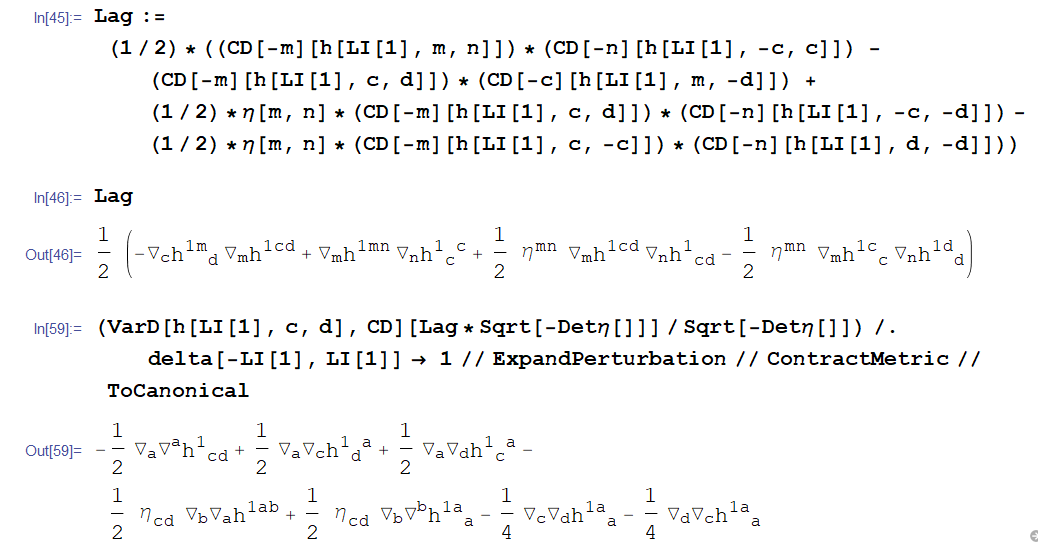
\includegraphics[scale=0.4]{lag-weak}
\end{figure}

Putting this back into \LaTeX{} after doing some manual contractions/simplifications, plus noting that the covariant derivative here is just the regular partial derivatives, we find that
\begin{align}
G_{\mu\nu} = \f{1}{2}\lp -\square h_{\mu\nu} + \p_\sigma \p_\nu \tensor{h}{^\sigma_\mu}  
+ \p_\sigma \p_\mu \tensor{h}{^\sigma_\nu} 
- \eta_{\mu\nu}\p_\lambda \p_\sigma h^{\lambda\sigma} + \eta_{\mu\nu}\square h - \p_\mu\p_\nu h\rp
\end{align}
which matches exactly with the Einstein tensor $G_{\mu\nu}$ provided earlier.\\


Note that when calling the perturbation metric $h_{\mu\nu}$ in xACT, make sure that you are calling it by \textbf{h[LI[order],-m,-n]}, so that xACT knows you \textit{mean} to call the perturbation metric.\\



Thus we confirm that the Lagrangian above gives the correct Einstein tensor. But how is it found? Consider a general coordinate transformation:
\begin{align}
x'^\mu \to x^\mu - \epsilon^\mu(x).
\end{align}
Then the metric changes according to 
\begin{align}
g'^{\mu\nu} = \f{\p x'^\mu}{\p x^a} \f{\p x'^\nu}{\p x^b} g^{ab},
\end{align}
where, as before,
\begin{align}
g^{\mu\nu} = \eta^{\mu\nu} - h^{\mu\nu} +\dots
\end{align}
How does $h_{\mu\nu}$ transform under this transformation? Well, we first have that
\begin{align}
\f{\p x'^\mu}{\p x^a}= \f{\p}{\p x^a} (x^\mu - \epsilon^\mu(x)) = \delta^\mu_a - \p_a \epsilon^\mu.
\end{align}
And so treating $\p_\mu \epsilon_\nu$ as the same order as $h^{\mu\nu}$ we find
\begin{align}
g'^{\mu\nu} &= \f{\p x'^\mu}{\p x^a} \f{\p x'^\nu}{\p x^b}\lp \eta^{ab} - h^{ab} \rp\nn\\
&= (\delta^\mu_a - \p_a\epsilon^\mu)(\delta^\nu_b - \p_b\epsilon^\nu)\lp \eta^{ab} - h^{ab} \rp\nn\\
&\approx (\delta^\mu_a - \p_a\epsilon^\mu)(\eta^{a\nu} - h^{a\nu} - (\p_b e^\nu)\eta^{ab}+\dots\nn)\\
&\approx \eta^{\mu\nu} - h^{\mu\nu} - (\p_a \epsilon^\nu)\eta^{\mu a} - (\p_b \epsilon^\mu)\eta^{b\nu}.
\end{align}
Next, we lower the index to get $h'_{\mu\nu}$:
\begin{align}
\eta_{c\mu}\eta_{d\nu}g'^{\mu\nu} &= \eta_{c\mu}\eta_{d\nu}\lp \eta^{\mu\nu} - h^{\mu\nu} - (\p_a \epsilon^\nu)\eta^{\mu a} - (\p_b \epsilon^\mu)\eta^{b\nu} \rp\nn\\
\eta_{cd} - h'_{cd} &= \eta_{cd} - h_{cd} - (\p_a \epsilon_d)\delta^a_c - (\p_b\epsilon_c)\delta^b_c\nn\\
h'_{cd} &= h_{cd} + \p_c \epsilon_d +  \p_d \epsilon_c. 
\end{align}
And so we have
\begin{align}
\boxed{h'_{\mu\nu}= h_{\mu\nu} + \p_\mu \epsilon_\nu + \p_\nu \epsilon_\mu}
\end{align}
and of course as a side product:
\begin{align}
\boxed{h'^{\mu\nu} = h^{\mu\nu} + \p^\mu \epsilon^\nu + \p^\nu \epsilon^\mu}
\end{align}
and so the infinitesimal change in $h_{ab}$ or $h^{ab}$ is
\begin{align}
&\boxed{\delta h_{\mu\nu} = \p_\mu \epsilon_\nu + \p_\nu \epsilon_\mu}\\
&\boxed{\delta h^{\mu\nu} = \p^\mu \epsilon^\nu + \p^\mu \epsilon^\mu}
\end{align}
which, by the way, are actually the Lie derivatives of the perturbative metric $h_{\mu\nu}$ and its inverse $h^{\mu\nu}$. These formulas represent the change of the metric perturbation under an infinitesimal diffeomorphism along the vector field $\epsilon^\mu$. \\ 

Since we want to get $G_{\mu\nu}$ that is linear in $h_{\mu\nu}$, we look for quadratic terms in $h$ and in $\p$. Lorentz invariance tells us that there are four possible terms. So the action has the form
\begin{align}
\boxed{S = \int d^4x\,(a\p_\lambda h^{\mu\nu}\p^\lambda h_{\mu\nu} + b \p_\lambda \tensor{h}{^\mu_\mu} \p^\lambda \tensor{h}{^\nu_\nu} + c\p_\lambda h^{\lambda \nu}\p^\mu h_{\mu\nu} + d\p^\mu\tensor{h}{^\lambda_\lambda}\p^\nu h_{\mu\nu} )}
\end{align}
where $a,b,c,d$ are unknown constants. Next, we require that $\delta S / \delta h_{\mu\nu} =0 $ with $\delta h_{\mu\nu} = \p_\mu \epsilon_\nu + \p_\nu \epsilon_\mu$. This should give 3 equations with 4 unknowns. Upon writing three unknowns in terms of the remaining unknown we can find the form of the Lagrangian. In the end, we should be able to fix the action up to an overall constant factor.\\

With $\delta S = 0$, we bring the $\delta$ into the integrand and let $\delta \lag = 0$. The next step is to do variational derivatives with respect to $h_{\mu\nu}$ on each term in the integrand. We shall proceed, first with the first term:
\begin{align}
\delta(\p_\lambda h^{\mu\nu}\p^\lambda h_{\mu\nu}) &= \p_\lambda (\delta h^{\mu\nu})(\p^\lambda h_{\mu\nu}) + (\p_\lambda h^{\mu\nu})\p^\lambda( \delta h_{\mu\nu} )\nn\\
&= \p_\lambda (\p^\mu \epsilon^\nu + \p^\nu \epsilon^\mu)(\p^\lambda h_{\mu\nu}) + (\p_\lambda h^{\mu\nu})\p^\lambda (\p_\mu \epsilon_\nu + \p_\nu \epsilon_\mu)\nn\\
&= \p_\lambda (\p^\mu \epsilon^\nu + \p^\nu \epsilon^\mu)(\p^\lambda h_{\mu\nu}) + (\p^\lambda h_{\mu\nu})\p_\lambda (\p^\mu \epsilon^\nu + \p^\nu \epsilon^\mu)\nn\\
&= 2\p_\lambda (\p^\mu \epsilon^\nu + \p^\nu \epsilon^\mu)(\p^\lambda h_{\mu\nu})\nn\\
&= 4[\p_\lambda (\p^\mu \epsilon^\nu)](\p^\lambda h_{\mu\nu}),
\end{align}
where the fourth equality follows from the symmetry $\mu\leftrightarrow \nu$ in a summation. Zee says 
\begin{align}
[\p_\lambda (\p^\mu \epsilon^\nu)](\p^\lambda h_{\mu\nu}) \sim \epsilon^\nu \p^2 \p^\mu h_{\mu\nu}
\end{align}
from ``integrating by parts'' freely. It turns out we have to integrate by parts twice to get this equality. We shall proceed with the first integration by parts with respect to some measure $d\omega$ which we are not going to worry about. We shall also assume that everything vanishes when evaluated at infinity and that differential operators such as $\delta, \p_\alpha, \p^\beta, \square$ commute.
\begin{align}
\int d\omega \, \p_\lambda[(\p^\mu \epsilon^\nu)(\p^\lambda h_{\mu\nu})] &= \int d\omega\, [\p_\lambda(\p^\mu\epsilon^\nu)](\p^\lambda h_{\mu\nu}) + \int d\omega\, (\p^\mu\epsilon^\nu)(\p_\lambda \p^\lambda h_{\mu\nu}) \nn\\
(\p^\mu \epsilon^\nu)(\p^\lambda h_{\mu\nu})\bigg\vert_{-\infty}^\infty&= \int d\omega\, [\p_\lambda(\p^\mu\epsilon^\nu)](\p^\lambda h_{\mu\nu}) + \int d\omega\, (\p^\mu\epsilon^\nu)(\p_\lambda \p^\lambda h_{\mu\nu})\nn\\
0  &=  \int d\omega\, [\p_\lambda(\p^\mu\epsilon^\nu)](\p^\lambda h_{\mu\nu}) + \int d\omega\, (\p^\mu\epsilon^\nu)(\p_\lambda \p^\lambda h_{\mu\nu})\nn\\
\implies [\p_\lambda(\p^\mu \epsilon^\nu)] (\p^\lambda h_{\mu\nu})  &= -\p^\mu \epsilon^\nu \p_\lambda \p^\lambda h_{\mu\nu}.
\end{align}
We evaluate this term (again) by integration by parts, again over some arbitrary measure $d\omega$ we won't worry about:
\begin{align}
\p^\mu (\epsilon^\nu \p_\lambda \p^\lambda h_{\mu\nu})\bigg\vert_{-\infty}^\infty &= \int d\omega\, \p^\mu \epsilon^\nu \p_\lambda \p^\lambda h_{\mu\nu} + \int d\omega\,  \epsilon^\nu \p_\lambda \p^\lambda \p^\mu h_{\mu\nu}\nn\\
0 &= \int d\omega\, \p^\mu \epsilon^\nu \p_\lambda \p^\lambda h_{\mu\nu} + \int d\omega\,  \epsilon^\nu \p_\lambda \p^\lambda \p^\mu h_{\mu\nu}\nn\\
\implies -\p^\mu \epsilon^\nu \p_\lambda \p^\lambda h_{\mu\nu} &= \epsilon^\nu \underbrace{\p_\lambda \p^\lambda}_{\square} \p^\mu h_{\mu\nu}.
\end{align}
And so, we have for the first term:
\begin{align}
\boxed{\delta (\p_\lambda h^{\mu\nu} \p^\lambda h_{\mu\nu}) = 4e^\nu \square \p^\mu h_{\mu\nu}} 
\end{align}


Moving on the second term:
\begin{align}
\delta[(\p_\lambda h)( \p^\lambda h)] &= \delta[(\p_\lambda \tensor{h}{^\mu_\mu})( \p^\lambda \tensor{h}{^\nu_\nu})]\nn\\
&= (\p_\lambda \delta\tensor{h}{^\mu_\mu})( \p^\lambda \tensor{h}{^\nu_\nu}) + (\p_\lambda \tensor{h}{^\mu_\mu})( \p^\lambda \delta\tensor{h}{^\nu_\nu}).
\end{align}
We notice that this term is very similar to the first term, except for the ``position of the index of $h$.'' That is to say, we are finding $\delta$ of the contraction. However, we can always write
\begin{align}
&\tensor{h}{^\mu_\mu} = \eta_{\mu x}h^{\mu x}\\
&\tensor{h}{^\nu_\nu} = \eta^{\nu y}h_{\nu y}.
\end{align}
From here we can do some mental prepping for what to come: the metric is constant in the eyes of $\delta$, so we can just pull the $\eta$'s out to the left and treat them as constants. By doing this, we're left with $\eta^{\mu x}\eta_{\nu y}$ times a term of the form similar to the first term except for the appearance of the indices $x,y$. However, by symmetry arguments, we should be able to get
\begin{align}
\delta[(\p_\lambda h)( \p^\lambda h)] = 4\epsilon^\nu \square \p_\nu h
\end{align}
where the factor of $4$ is explicitly shown here for reasons we will see later. We shall see why this is true. First we write the contractions in terms of the original tensor $h$ times the metric 
\begin{align}
\delta[(\p_\lambda h)( \p^\lambda h)] &= \lp\eta_{\mu x}\eta^{\nu y}\rp\delta[(\p_\lambda h^{\mu x})(\p^\lambda h_{\nu y})].
\end{align}
Invoking the fact that
\begin{align}
&\delta h^{ab} = \p^a \epsilon^b + \p^b \epsilon^a \nn\\
&\delta h_{ab} = \p_a \epsilon_b + \p_b \epsilon_a 
\end{align}
and the $b\leftrightarrow a$ symmetry argument in a summation, we find
\begin{align}
\delta[(\p_\lambda h)( \p^\lambda h)] &= 2\lp\eta_{\mu x}\eta^{\nu y}\rp [(\p_\lambda \p^\mu \epsilon^x)(\p^\lambda h_{\nu y}) + (\p^\lambda h_{\mu x})(\p_\lambda \p^\nu \epsilon^y)]\nn\\
&= 2\lp\eta_{\mu x}\eta^{\nu y}\rp [(\p_\lambda \p^\mu \epsilon^x)(\p^\lambda h_{\nu y}) + (\p_\lambda h^{\mu x})(\p^\lambda \p_\nu \epsilon_y)]\nn\\
&= 4\lp\eta_{\mu x}\eta^{\nu y}\rp[(\p_\lambda \p^\mu \epsilon^x)(\p^\lambda h_{\nu y})]\nn\\
&= 4(\p_\lambda \p^\mu \epsilon_\mu)(\p^\lambda h)\nn\\
&= 4(\p_\lambda \p_\mu \epsilon^\mu)(\p^\lambda h).
\end{align}
Time to integrate by parts (again over some measure $d\omega$ we won't worry about)
\begin{align}
\p_\lambda[(\p_\mu \epsilon^\mu)(\p^\lambda h)]\bigg\vert_{-\infty}^\infty  &= \int d\omega\,(\p_\lambda \p_\mu \epsilon^\mu)(\p^\lambda h) + \int d\omega\,(\p_\mu \epsilon^\mu)\square h\nn\\
0 &= \int d\omega\,(\p_\lambda \p_\mu \epsilon^\mu)(\p^\lambda h) + \int d\omega\,(\p_\mu \epsilon^\mu)\square h\nn\\
\implies (\p_\lambda \p_\mu \epsilon^\mu)(\p^\mu h) &= -(\p_\mu \epsilon^\mu)\square h.
\end{align}
We integrate by parts again:
\begin{align}
\p_\mu[\epsilon^\mu \square h]\bigg\vert_{-\infty}^\infty &= \int d\omega\,(\p_\mu \epsilon^\mu)\square h + \int d\omega\, e^\mu \square \p_\mu h\nn\\
0 &= \int d\omega\,(\p_\mu \epsilon^\mu)\square h + \int d\omega\, \epsilon^\mu \square \p_\mu h\nn\\
\implies (\p_\mu \epsilon^\mu)\square h &=-\epsilon^\mu \square \p_\mu h.
\end{align}
So we have for the second term
\begin{align}
\boxed{\delta[(\p_\lambda h)( \p^\lambda h)] = 4\epsilon^\nu \square \p_\nu h}
\end{align}
Very nice! What about the third term? We claim:
\begin{align}
\delta[(\p_\lambda h^{\lambda \nu})( \p^\mu h_{\mu\nu})] = 2\epsilon^\nu\square\p^\mu h_{\mu\nu} + 2\epsilon^\nu \p_\nu \p^\lambda  \p^\mu h_{\mu\lambda}.
\end{align}
The only way to verify this is integration by parts (surprise!). But first we have to let $\delta$ act on the $h$'s and write things out in terms of $\epsilon$'s:
\begin{align}
\delta[(\p_\lambda h^{\lambda \nu})( \p^\mu h_{\mu\nu})] = (\p_\lambda(\p^\lambda \epsilon^\nu + \p^\nu \epsilon^\lambda))(\p^\mu h_{\mu\nu}) + (\p_\lambda h^{\lambda\nu})(\p^\mu(\p_\mu \epsilon_\nu + \p_\nu \epsilon_\mu)).
\end{align}
We will treat these two terms differently, despite the symmetry. For the first term, we simply integrate by parts twice to get
\begin{align}
(\p_\lambda(\p^\lambda \epsilon^\nu + \p^\nu \epsilon^\lambda))(\p^\mu h_{\mu\nu}) &= 2(\p_\lambda\p^\lambda \epsilon^\nu)(\p^\mu h_{\mu\nu}) \nn\\
&= -2(\p^\lambda \epsilon^\nu)(\p_\lambda\p^\mu h_{\mu\nu}) \nn\\
&= 2(\epsilon^\nu)(\p^\lambda \p_\lambda\p^\mu h_{\mu\nu})\nn\\
&= 2(\epsilon^\nu)\square\p^\mu h_{\mu\nu}.
\end{align}
We recognize that, for the second term, by exchanging the indices  $\mu \to \nu \to \lambda \to \mu$, then appropriately lowering and raising the indices on the second term, then use the $\lambda \leftrightarrow \nu$ symmetry argument in the Lie derivative summation, we get
\begin{align}
(\p_\mu h^{\mu\lambda})(\p^\nu(\p_\lambda \epsilon_\nu + \p_\nu \epsilon_\lambda)) &= (\p^\mu h_{\mu\lambda})(\p_\nu(\p^\lambda \epsilon^\nu + \p^\nu \epsilon^\lambda))\nn\\
&= 2(\p^\mu h_{\mu\lambda})(\p_\nu\p^\lambda \epsilon^\nu).
\end{align}
From here, we will integrate by parts twice to get what we want. I won't be showing all the steps here because we can now do this integration by parts ``internally:''
\begin{align}
2(\p^\mu h_{\mu\lambda})\p_\nu (\p^\lambda \epsilon^\nu) = -2(\p_\nu\p^\mu h_{\mu\lambda})(\p^\lambda \epsilon^\nu) = 2\epsilon^\nu \p^\lambda \p_\nu \p^\mu h_{\mu\lambda} = 2\epsilon^\nu \p_\nu \p^\lambda  \p^\mu h_{\mu\lambda},
\end{align} 
where the last equality follows from the fact that these differential operators commute. Recognize the pattern in the first two equalities? Every time we integrate by parts, we essentially let one derivative act on another factor (say let $\p_\nu$ act on the $\p h$ instead of on $\epsilon$). Since the total derivative is zero when evaluated at infinity, this new quantity is equal to minus the original quantity. We keep doing this until all derivatives are sandwiched between $\epsilon^\nu$ and $h_{\mu\lambda}$. \\

So we have for the third term
\begin{align}
\boxed{\delta[(\p_\lambda h^{\lambda \nu})( \p^\mu h_{\mu\nu})] = 2\epsilon^\nu\square\p^\mu h_{\mu\nu} + 2\epsilon^\nu \p_\nu \p^\lambda  \p^\mu h_{\mu\lambda}}
\end{align}

What about the fourth term? Once again we have a contraction, which means we need to write it out in terms of the metric $\eta$, then pull it outside of the derivative since it is just a constant in the eyes of $\delta$. We also invoke the symmetry argument once again with derivatives of the $\epsilon$'s. So,
\begin{align}
\delta[\p^\mu\tensor{h}{^\lambda_\lambda}\p^\nu h_{\mu\nu} ] &= \delta[\eta_{\lambda x}\p^\mu h^{\lambda x}  \p^\nu h_{\mu\nu}]\nn\\
&= (\eta_{\lambda x})\delta[ \p^\mu h^{\lambda x} \p^\nu h_{\mu\nu}]\nn\\
&= (\eta_{\lambda x})\lc \p^\mu(\p^\lambda \epsilon^x + \p^x \epsilon^\lambda)\p^\nu h_{\mu\nu} + \p^\mu h^{\lambda x}  \p^\nu (\p_\mu \epsilon_\nu + \p_\nu \epsilon_\mu) \rc\nn\\
&= 2(\p^\mu\p^\lambda \epsilon_\lambda) \p^\nu h_{\mu\nu} + (2\p^\mu h) \p^\nu(\p_\mu\epsilon_\nu).
\end{align}
Integrate by parts the first term (twice) to get
\begin{align}
2 (\p^\mu \p^\lambda \epsilon_\lambda)\p^\nu h_{\mu\nu} = 2\epsilon_\lambda \p^\lambda \p^\mu \p^\nu h_{\mu\nu}.
\end{align}
Integrate by parts the second term (twice) to get
\begin{align}
(2\p^\mu h) \p^\nu(\p_\mu\epsilon_\nu) &= 2\epsilon^\nu \square \p_\nu h.
\end{align}
So we have
\begin{align}
\boxed{\delta[\p^\mu\tensor{h}{^\lambda_\lambda} \p^\nu h_{\mu\nu}] = 2\epsilon_\lambda \p^\lambda \p^\mu \p^\nu h_{\mu\nu} + 2\epsilon_\nu\square \p^\nu h =  2\epsilon^\lambda \p_\lambda \p^\mu \p^\nu h_{\mu\nu}  + 2\epsilon^\nu\square \p_\nu h}
\end{align}
Very nice! Putting everything we've done so far together, we find
\begin{align}
&\,\delta(a\p_\lambda h^{\mu\nu}\p^\lambda h_{\mu\nu} + b \p_\lambda h \p^\lambda h + c\p_\lambda h^{\lambda \nu}\p^\mu h_{\mu\nu} + d\p^\mu h \p^\nu h )\nn\\
= &\,4a(\epsilon^\nu \square \p^\mu h_{\mu\nu}) + 4b(\epsilon^\nu \square \p_\nu h) + c (2\epsilon^\nu\square\p^\mu h_{\mu\nu} + 2\epsilon^\nu \p_\nu \p^\lambda  \p^\mu h_{\mu\lambda}) \nn \\ &\,\,\,\,\,+ 2d(\epsilon^\lambda \p_\lambda \p^\mu\p^\nu h_{\mu\nu}) + 2d(\epsilon^\nu \square \p_\nu h)\nn\\
= &\,(4a+2c)(\epsilon^\nu \square \p^\mu h_{\mu\nu}) + (4b + 2d)(\epsilon^\nu \square \p_\nu h) + (2c+ 2d)(\epsilon^\nu \p_\nu \p^\lambda\p^\mu h_{\lambda\mu})\nn\\
= & \,0.
\end{align} 
When holds when we let $a = 1/2$, then $c = -1$, so $d = 1$, which implies $b = -1/2$.
Thus the correct action up to an overall factor is
\begin{align}
\boxed{S = \int d^4x\, \f{1}{2}\p_\lambda h^{\mu\nu}\p^\lambda h_{\mu\nu} -\f{1}{2} \p_\lambda h \p^\lambda h -\p_\lambda h^{\lambda \nu}\p^\mu h_{\mu\nu} + \p^\mu h\p^\nu h}
\end{align}
So we have successfully constructed the linearized action.\\

Thus even if we had never heard of the Einstein-Hilbert action we could still determine the action gravity in the weak field limit by requiring that the action be invariant under the transformation
\begin{align}
x^\mu \to x'^\mu - \epsilon^\mu(x)
\end{align}
or equivalently 
\begin{align}
\delta h_{\mu\nu} = h'_{\mu\nu} - h_{\mu\nu} = \p_\mu \epsilon_\nu +\p_\nu \epsilon_\mu. 
\end{align}
So based on our argument in the previous section, we can now write the weak field expansion of the action $S$ as
\begin{align}
\boxed{S_{\text{wfg}} = \int d^4x\, \lp \f{1}{32\pi G}\mathcal{I} - \f{1}{2}h_{\mu\nu}T^{\mu\nu} \rp}
\end{align}
where
\begin{align}
\mathcal{I} = \f{1}{2}\p_\lambda h^{\mu\nu}\p^\lambda h_{\mu\nu} -\f{1}{2} \p_\lambda h \p^\lambda h -\p_\lambda h^{\lambda \nu}\p^\mu h_{\mu\nu} + \p^\mu h\p^\nu h
\end{align}
and $T_{\mu\nu}$ is the stress-energy tensor associated with matter. 






\subsubsection{Graviton propagator}


From the previous section we see that the weak field action $S_{\text{wfg}}$ has the same quadratic structure of all the field theories we have studied, and so the graviton propagator is once again the inverse of a differential operator. But just as in Maxwell's theory the relevant differential operator in the Einstein-Hilbert theory does not have an inverse because of the ``gauge invariance,'' i.e., under a transformation the action remains invariant. In other terms, we see that the kernel of the differential operator is not trivial, i.e., it is not one-to-one and therefore cannot have a well-defined inverse. \\

To deal with this, we need to rely on the Faddeev-Popov method. Recall that the Faddeev-Popov method allows us to split our integration over physically distinct configurations and those over gauge orbits.\\

We observe that by adding 
\begin{align}
\lp \p^\mu h_{\mu\nu} - \f{1}{2}\p_\nu \tensor{h}{^\lambda_\lambda} \rp^2
\end{align}
to the invariant Lagrangian
\begin{align}
\f{1}{2}\p_\lambda h^{\mu\nu}\p^\lambda h_{\mu\nu} -\f{1}{2} \p_\lambda \tensor{h}{^\mu_\mu} \p^\lambda \tensor{h}{^\nu_\nu} -\p_\lambda h^{\lambda \nu}\p^\mu h_{\mu\nu} + \p^\mu \tensor{h}{^\lambda_\lambda}\p^\nu h_{\mu\nu}
\end{align}
we get
\begin{align}
&\,\f{1}{2}\p_\lambda h^{\mu\nu}\p^\lambda h_{\mu\nu} -\f{1}{2} \p_\lambda \tensor{h}{^\mu_\mu} \p^\lambda \tensor{h}{^\nu_\nu} -\cancel{\p_\lambda h^{\lambda \nu}\p^\mu h_{\mu\nu}} + \cancel{\p^\mu \tensor{h}{^\lambda_\lambda}\p^\nu h_{\mu\nu}}\nn\\
&\,\,\,\,\,+ \cancel{(\p^\mu h_{\mu\nu})(\p^\lambda h_{\lambda \nu})} - \cancel{\p^\mu h_{\mu\nu}\p_\nu \tensor{h}{^\lambda_\lambda}} + \f{1}{4}(\p_\nu h)(\p^\nu h)\nn\\
=&\, \f{1}{2}\p_\lambda h^{\mu\nu}\p^\lambda h_{\mu\nu} -\f{1}{4} \p_\lambda \tensor{h}{^\mu_\mu} \p^\lambda \tensor{h}{^\nu_\nu}. 
\end{align}
the weak field action effectively becomes
\begin{align}
\boxed{S_\text{wfg} = \int d^4x\, \f{1}{2}\lb \f{1}{32\pi G}\lp \p_\lambda h^{\mu\nu} \p^\lambda h_{\mu\nu} - \f{1}{2}\p_\lambda h\p^\lambda h \rp - h_{\mu\nu}T^{\mu\nu} \rb}
\end{align}
Why is this addition justified? Recall in the subsection \textit{Gauge Invariance: A Photon Can Find No Rest} where we introduced the Faddeev-Popov trick, we find that by adding $(\p A)^2$ to the Lagrangian we were able to replace the original action by a new action whose Lagrangian contains has a differential operator with an inverse. We are doing a similar thing here. \\

But of course we can't just add whatever we want to the Lagrangian and expect it to describe the same physics. One way to keep the Lagrangian the same is to require whatever we are adding to be zero. In our case, the freedom in choosing $h_{\mu\nu}$ makes this a necessary condition, which means
\begin{align}
\p^\mu h_{\mu\nu} - \f{1}{2}\p_\nu \tensor{h}{^\lambda_\lambda}  = 0 \iff \boxed{\p^\mu h_{\mu\nu} = \f{1}{2}\p_\nu \tensor{h}{^\lambda_\lambda}}
\end{align} 
This is called the \textbf{harmonic gauge condition}. It turns out that this is the linearized version of
\begin{align}
\p_\mu \lp \sqrt{-g}g^{\mu\nu} \rp = 0.
\end{align}


With these results, we can write the action as
\begin{align}
S_\text{wfg} &= \int d^4x\, \f{1}{2}\lb \f{1}{32\pi G}\lp \p_\lambda h^{\mu\nu} \p^\lambda h_{\mu\nu} - \f{1}{2}\p_\lambda h\p^\lambda h \rp - h_{\mu\nu}T^{\mu\nu} \rb\nn\\
%&= \int d^4x\, \f{1}{2}\lb \f{1}{32\pi G}\lp \p_\lambda h^{\mu\nu} \p^\lambda h_{\mu\nu} - \p^\mu h_{\mu\nu} \p^\lambda h \rp - h_{\mu\nu}T^{\mu\nu} \rb\nn\\
&= \boxed{\f{1}{32\pi G}\int d^4x\, \lb h^{\mu\nu}K_{\mu\nu;\lambda\sigma}(-\p^2)h^{\lambda\sigma} + \mathcal{O}(h^3) \rb}
\end{align}
where
\begin{align}
\boxed{K_{\mu\nu;\lambda\sigma} \equiv \f{1}{2}(\eta_{\mu\lambda}\eta_{\nu\sigma} +\eta_{\mu\sigma}\eta_{\nu\lambda} - \eta_{\mu\nu}\eta_{\lambda\sigma}  )}
\end{align}
where we regard $\lambda\nu$ and $\lambda\sigma$ as two indices. We can work backwards to check writing the action in this form makes sense, but let's not worry too much about that for now.\\

Note that we are dealing with matrices acting in a linear space spanned by symmetric two-index tensors. Thus, the identity matrix is actually
\begin{align}
I_{\mu\nu;\lambda\sigma} \equiv \f{1}{2}(\eta_{\mu\lambda}\eta_{\nu\sigma} + \eta_{\mu\sigma}\eta_{\nu\sigma}).
\end{align}
We can check that
\begin{align}
K_{\mu\nu;\lambda\sigma} \tensor{K}{^{\lambda\sigma}_{;\rho\omega}} = I_{\mu\nu;\rho\omega},
\end{align}
so that
\begin{align}
K^{-1} = K,
\end{align}
similar to how $\eta^{\mu\nu} = \eta_{\mu\nu}$. Thus in the harmonic gauge the graviton propagator in flat spacetime, in momentum space, is given by (up to Newton's constant)
\begin{align}
\boxed{\D_{\mu\nu;\lambda\sigma}(k) = \f{1}{2}\f{K_{\mu\nu;\lambda\sigma}}{k^2 + i\epsilon} = \f{1}{2}\f{\eta_{\mu\lambda}\eta_{\nu\sigma} +\eta_{\mu\sigma}\eta_{\nu\lambda} - \eta_{\mu\nu}\eta_{\lambda\sigma}}{k^2 + i\epsilon}}
\end{align}
where the final $k^2$ comes from the $\p^2$ in the Lagrangian when moving to momentum space, as always.  \\

So there is our graviton propagator, in the weak field limit.




\subsubsection{Newton from Einstein}

Suppose we want to find the equation of motion corresponding to the action given above
\begin{align}
S_\text{wfg} &= \int d^4x\, \f{1}{2}\lb \f{1}{32\pi G}\lp \p_\lambda h^{\mu\nu} \p^\lambda h_{\mu\nu} - \f{1}{2}\p_\lambda h\p^\lambda h \rp - h_{\mu\nu}T^{\mu\nu} \rb.
\end{align}
To find the equation of motion for this theory we take the variational derivative of $S_\text{wfg}$ with respect to $h^{\mu\nu}$. \\

We will rely on xACT to do this. Assuming that the rest has been setup correctly, we will just define the effective Lagrangian, vary it with respect to $h_{\mu\nu}$, and set everything to zero.
\begin{lstlisting}
In[15]:= DefTensor[T[m, n], M4]

During evaluation of In[15]:= ** DefTensor: Defining tensor T[m,n]. 

In[16]:= DefConstantSymbol[G]

During evaluation of In[16]:= ** DefConstantSymbol: Defining constant symbol G. 

In[19]:= LagEff := (1/
2)*( (1/(32*Pi*G))*(CD[-l][h[LI[1], m, n]]*
CD[l][h[LI[1], -m, -n]] - (1/2)*CD[-l][h[LI[1], a, -a]]*
CD[l][h[LI[1], b, -b]]) - h[LI[1], -m, -n]*T[m, n] )

In[20]:= LagEff

Out[20]= 1/2 (- h[
xAct`xTensor`LI[1], -m, -n]  T[m, n] + (-(1/2) CD[-l][
h[
xAct`xTensor`LI[1], a, -a]] CD[l][
h[
xAct`xTensor`LI[1], b, -b]] + CD[-l][
h[
xAct`xTensor`LI[1], m, n]] CD[l][
h[
xAct`xTensor`LI[1], -m, -n]])/(32 G \[Pi]))

In[23]:= (VarD[h[LI[1], c, d], CD][LagEff*Sqrt[-Det\[Eta][]]]/
Sqrt[-Det\[Eta][]]) == 0 /. delta[-LI[1], LI[1]] -> 1 // 
ExpandPerturbation // ContractMetric // ToCanonical
\end{lstlisting}
We quickly find
\begin{figure}[!htb]
	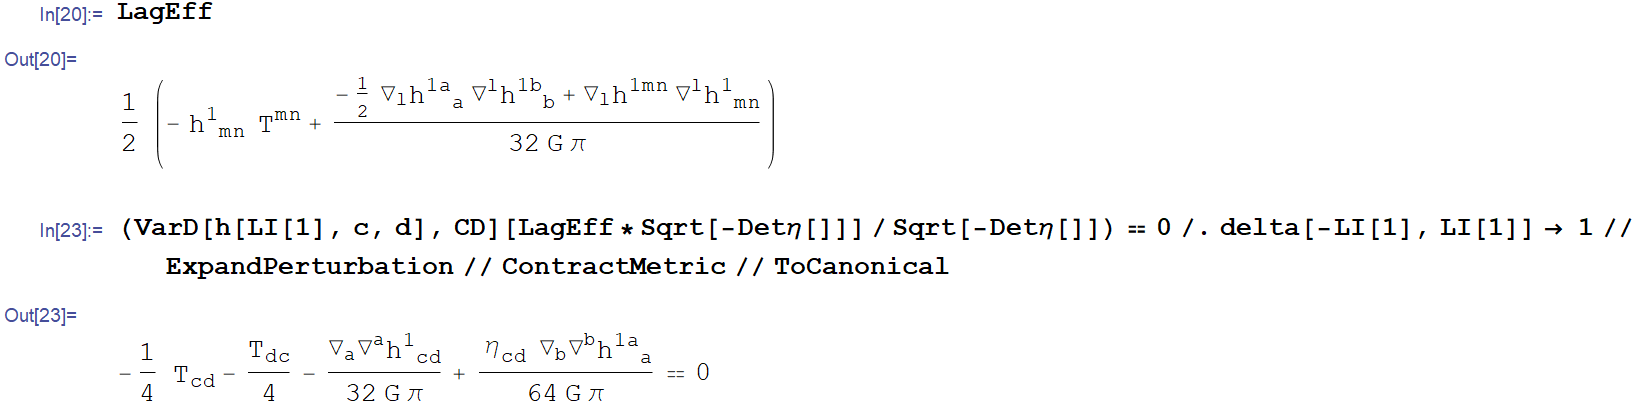
\includegraphics[scale=0.3]{newton-einstein}
\end{figure}
Since the stress-energy tensor is symmetric, we can combine $T_{cd}$ and $T_{dc}$ in the output to get the Euler-Lagrange equation of motion:
\begin{align}
\boxed{\f{1}{32\pi G}(- 2 \square h_{\mu\nu} + \eta_{\mu\nu} \square h) - T_{\mu\nu} = 0}
\end{align}
Easy! Contracting this (i.e., taking the trace):
\begin{align}
\eta_{\mu\nu}\lb\f{1}{32\pi G}(- 2 \square h_{\mu\nu} + \eta_{\mu\nu} \square h) - T_{\mu\nu}\rb &= \f{1}{32\pi G}\lp -2\square h + 4 \square h \rp - T \nn\\
&= \f{1}{16\pi G} \square h - T \nn\\
&= 0.
\end{align}
Therefore
\begin{align}
\square h = 16\pi GT = 16\pi G \eta^{\mu\nu}T_{\mu\nu}.
\end{align}
And so plugging things back into the Euler-Lagrange equation we can find 
\begin{align}
\boxed{\square h_{\mu\nu} = -16\pi G \lp T_{\mu\nu} - \f{1}{2}\eta_{\mu\nu}T \rp}
\end{align}
In the static limit, $T_{00}$ is the dominant component of the stress-energy tensor, and so this equality reduces to
\begin{align}
\boxed{\laplacian{\phi}= 4\pi GT_{00}}
\end{align}
where the Newtonian gravitational potential is $\phi \equiv h_{00}/2$. We have just derived Poisson's equation for $\phi$.











\newpage













\section{Massive Gravity}

\subsection{A Brief History}

Massive gravity has a long-winded history. In 1939, Fierz-Pauli wrote down a linearized massive gravity theory for massive spin-2 field $h_{\mu\nu}$. ($j = 2, m_j = -2,-1,0,1,2$). \\

Later in 1970, van Dam, Veltman, and Zakharov (vDVZ) discovered what called the vDVZ discontinuity. They showed that in the $m\to 0$ limit, Fierz-Pauli theory no longer agrees with GR.\\

Then, in 1872 Vainshtein studied non-linear Fierz-Pauli and found a screening mechanism where near some object like the sun for $r < r_V \sim (M / m^4 M_{Pl}^2)^{1/5} = \Lambda_5$ agreement with GR is obtained in the $m \to 0$ limit. \\

In the same year, however, Boulware \& Desen showed that in the nonlinear regime, a ghost mode emerges (BD ghost).\\

In 2003, Arkani-Hamed et al wrote a expository \href{https://arxiv.org/pdf/hep-th/0210184.pdf}{\underline{paper}} on this theory. We will spend some time on this paper.\\

Then, in 2010, de Rham-Gabadadze-Tolley (dRGT) found that for a special non-linear potential in place of the Fierz-Pauli mass term the DB ghost goes away. This new theory is valid up to $\Lambda_5$ cutoff scale. This theory also has self-accelerating solutions. This implies less need for dark energy.



\newpage


\subsection{Quick review of Field Dimensions}
Here we will quickly go over basic field dimensions. We first establish the natural units: $\hbar = c = 1$. With this $E \sim m \sim p \sim \omega$ GeV. $x\sim t \sim 1/E$. We will use mass dimension $m$ as units. With this.
\begin{align}
[x] = [t] =  [K]^{-1} = m^{-1}.
\end{align} 
The action looks something like
\begin{align}
S = \int d^4x\, dt \lag.
\end{align}
$S$ has units of $\hbar = J\cdot s$, so $S$ has no units. So
\begin{align}
[S] = [K]^{0} = m^0.
\end{align}
We can figure out field dimensions from $S$. Relativistically,
\begin{align}
S = \int d^4x\,\lag.
\end{align}
The action is dimensionless, while $[d^4x] = [K]^{-4}$. So
\begin{align}
[\lag] = [K]^{4}.
\end{align}
Now suppose for the scalar field theory
\begin{align}
\lag = \p \phi \p \phi
\end{align}
schematically. Then because $[\p] = [t]^{-1} = [x]^{-1} = [K]$, we find that
\begin{align}
[\phi]= [K].
\end{align}
So, scalars have mass dimension of 1. \\

Next, we look at vector field theory with
\begin{align}
\lag \sim F^{\mu\nu}F_{\mu\nu}
\end{align}
where 
\begin{align}
F_{\mu\nu} = \p_\mu A_\nu - \p_\nu A_\mu.
\end{align}
Since $[\lag] = [K]^4$ and $[\p]= [K]$, we find
\begin{align}
[A_\mu] = [K].
\end{align}
So vector fields also have mass dimension 1. What about a mass term? Suppose
\begin{align}
\lag = \f{1}{2}\p_\mu \phi \p6\mu \phi- \f{1}{2}m^2 \phi^2.
\end{align}
We see that $[m] = [K] = m$ is consistent with $[\phi] = m$ and $[\lag] = [K]^4 = m^4$.\\

What about gravity? What is the dimension of the metric? Well, we look at
\begin{align}
ds^2 = g_{\mu\nu}dX^\mu dX^\nu.
\end{align}
There are two units of length on both sides of the equation so
\begin{align}
[g_{\mu\nu}] = [K]^0,
\end{align}
i.e. assuming Cartesian coordinates, the metric is dimensionless. What about the connections? Christoffel symbols have the form
\begin{align}
\Gamma \sim g \p g.
\end{align}
So 
\begin{align}
[\Gamma] = [\p] = [K].
\end{align}
Riemann curvature tensors look like
\begin{align}
\tensor{R}{^a_{bcd}} \sim \Gamma^2 + \p \Gamma + \dots
\end{align}
so 
\begin{align}
[\tensor{R}{^a_{bcd}}] = [K]^2.
\end{align}
So we find that 
\begin{align}
[\lag_{grav}] = [\tensor{R}{^\mu_\mu}] \neq [K]^4.
\end{align}
It turns out that
\begin{align}
[\lag] \sim \f{1}{16\pi G}[R] = [K]^4.
\end{align}
This means 
\begin{align}
[G] = [K]^{-2}.
\end{align}
This says the Newton's gravitational constant $G$ has mass$^{-2}$ units. With this we can define
\begin{align}
G \equiv \f{1}{m^2_{Pl}},
\end{align}
where $m_{Pl}$ is the Planck mass. In GeV units, $m_{Pl} \sim 10^{19}$ GeV, which is very large, making $G$ very small. \\

Lastly, we notice that gravity has a dimensional constant in its kinetic term, while other fields do not. This makes quantizing/renormalizing gravity difficult. 











\newpage
\subsection{Fierz-Pauli Massive Gravity}

This section focuses on various aspects of Fierz-Pauli massive gravity. The content is based on this \href{https://arxiv.org/abs/1105.3735}{\underline{paper}} by Kurt Hinterbichler. This is my exposition of part II. of the paper, which gives an overview of the original Fierz-Pauli massive gravity. I will follow the paper's layout through and fill in the details wherever I feel necessary.


\subsubsection{The Action \& Fierz-Pauli Tuning}



Recall from earlier we have worked both ways to show the action in linearized gravity (without $T_{\mu\nu}$) up to some overall constant factor is:
\begin{align}
S_{Zee} = \int d^Dx\, \f{1}{2}\p_\lambda h^{\mu\nu}\p^\lambda h_{\mu\nu} -\f{1}{2} \p_\lambda h \p^\lambda h -\p_\lambda h^{\lambda \nu}\p^\mu h_{\mu\nu} + \p^\mu h\p^\nu h_{\mu\nu}.
\end{align}
This is the action obtained from Zee's construction. But to stay close this paper, I will use Sean Carroll's action instead:
\begin{align}
S_{SC} = \int d^Dx\, -\f{1}{2}\p_\lambda h_{\mu\nu} \p^\lambda h^{\mu\nu} + \p_\mu h_{\nu\lambda}\p^\nu h^{\mu\lambda} - \p_\mu h^{\mu\nu}\p_\nu h + \f{1}{2}\p_\lambda h \p^\lambda h.
\end{align}
This action is exactly the same as what Carroll has, up to index permutations.\\

We are familiar with this action, as it describes the (well-known by now) weak field limit. The Fierz-Pauli action is just this with an additional mass term:
\begin{align}
\int d^Dx\, -\f{1}{2}m^2\lp h_{\mu\nu}h^{\mu\nu} - h^2 \rp
\end{align}
hence the name ``massive gravity.'' The full action, then, is
\begin{empheq}[box=\widefbox]{align}
S_{FP} = \int d^Dx\, &-\f{1}{2}\p_\lambda h_{\mu\nu} \p^\lambda h^{\mu\nu} + \p_\mu h_{\nu\lambda}\p^\nu h^{\mu\lambda}\nn\\& - \p_\mu h^{\mu\nu}\p_\nu h + \f{1}{2}\p_\lambda h \p^\lambda h -\f{1}{2}m^2\lp h_{\mu\nu}h^{\mu\nu} - h^2 \rp
\end{empheq}
We wish to show that this action describes a massive spin 2 field (5 d.o.f $= 2s+1$). In the $m=0$ case, we recover the linearized Einstein-Hilbert action with the gauge symmetry:
\begin{align}
\delta h_{\mu\nu} = \p_\mu \epsilon_\nu + \p_\nu \epsilon_\mu
\end{align}
where once again 
\begin{align}
\delta h_{\mu\nu} = h'_{\mu\nu} - h_{\mu\nu}. 
\end{align}
We have actually seen how the action can be constructed from this gauge symmetry.\\

With $m\neq 0$, however, the gauge symmetry is violated. It is clear that
\begin{align}
\delta\lb \f{1}{2}m^2\lp h^{\mu\nu}h_{\mu\nu} + h^2 \rp  \rb &= \f{1}{2}m^2 \lb (\p^\mu \epsilon^\nu + \p^\nu \epsilon^\mu)h_{\mu\nu} + h^{\mu\nu}(\p_\mu\epsilon_\nu + \p_\nu\epsilon_\mu ) - \delta h^2 \rb\nn\\
&= \f{1}{2}m^2\lb 2(\p^\mu \epsilon^\nu + \p^\nu \epsilon^\mu)h_{\mu\nu} - \delta(\tensor{h}{^\mu_\mu}\tensor{h}{^\nu_\nu}) \rb\nn\\
&= \f{1}{2}m^2\lb 4(\p^\mu \epsilon^\nu) h_{\mu\nu} - \eta_{\mu a}\eta^{\nu b}\delta(h^{\mu a}h_{\nu b}) \rb\nn\\
&= \f{1}{2}m^2\lb 4(\p^\mu \epsilon^\nu) h_{\mu\nu} - \eta_{\mu a}\eta^{\nu b}\lc 2(\p^\mu\epsilon^a)h_{\nu b} + 2(\p_\nu \epsilon_b)h^{\mu a}\rc \rb\nn\\
&= \f{1}{2}m^2\lb 4(\p^\mu \epsilon^\nu) h_{\mu\nu} - 4(\p^\mu \epsilon_\mu)h \rb\nn\\
&= 2m^2[(\p^\mu \epsilon^\nu) h_{\mu\nu} - (\p^\mu \epsilon_\mu)h],
\end{align}
which is linearly independent with other terms in the variational Lagrangian $\delta \lag$. This says that
\begin{align}
\delta \lag = 0 \iff m^2 = 0.
\end{align}
But obviously since we explicitly set $m\neq 0$, we must have that $\delta \lag \neq 0$ under $\delta h_{\mu\nu} = \p_\mu \epsilon_\nu + \p_\nu \epsilon_\mu$. So we say the mass term violates this gauge symmetry.\\

The relative coefficient $-1$ between $h^2$ and $h_{\mu\nu}h^{\mu\nu}$ contractions is called the \textit{Fierz-Pauli tuning}. This number is not enforced by any known symmetry. However, any deviation from it, i.e., for any combination
\begin{align}
h_{\mu\nu}h^{\mu\nu} - (1-a)h^2, \quad a \neq 0
\end{align}
results in the action describing a scalar ghost with mass
\begin{align}
\boxed{m_g^2 = -\f{3-4a}{2a}m^2}
\end{align}
and negative kinetic energy in addition to the massive spin 2. We shall show why this is the case with a 2-step argument partially inspired by \href{http://indico.ictp.it/event/a11178/session/6/contribution/3/material/0/0.pdf}{\underline{A. Nicolis}} from ICTP. In Step 1, we show that the Fierz-Pauli tuning has to be $-1$ to avoid ghosts. In Step 2, we argue how the ghost of $m_{g}^2$ is obtained when $a\neq 0$ by a Hamiltonian analysis, inspired by \href{https://arxiv.org/pdf/1105.3735.pdf}{\underline{Kurt Hinterbichler}} and \href{https://digitalcommons.colby.edu/cgi/viewcontent.cgi?article=1721&context=honorstheses}{Greg Seyfarth}. \\


\textit{Step 1:} To this end, we consider the action (without matter, i.e., $T^{\mu\nu} = 0$) of the form
\begin{align}
S = \int d^Dx\, \lb\lag_{m=0,\text{linear}} - \f{1}{2}m^2(h_{\mu\nu}h^{\mu\nu} - (1-a)h^2)\rb
\end{align}

The linearized equations of motion follow from varying the action with respect to $h_{\mu\nu}$. The linearized Lagrangian gives the Einstein tensor (without matter) $G_{\mu\nu}$, while the massive terms gives 
\begin{align}
\f{\delta}{\delta h_{\mu\nu}} \lc \f{1}{2}m^2\lp h_{\mu\nu}h^{\mu\nu} - (1-a)h^2 \rp \rc &=
\f{1}{2}m^2 \lp h^{\mu\nu} - (1-a) h \eta^{\mu\nu} h_{\mu\nu} \rp\nn\\
&= \f{1}{2}m^2 \lp h^{\mu\nu} - (1-a)\eta^{\mu\nu} h \rp.
\end{align}
Covariantly, (to match the lower indices of $G_{\mu\nu}$), this is 
\begin{align}
-\f{1}{2}m^2 \lp h_{\mu\nu} - (1-a)\eta_{\mu\nu} h \rp.
\end{align}
So the equation of motion reads
\begin{align}
\boxed{G_{\mu\nu, \text{linear}} + \f{1}{2}m^2 \lp h_{\mu\nu} - (1-a)\eta_{\mu\nu}h \rp = 0}
\end{align}
(Notice that we have made no assumptions about $\delta h_{\mu\nu}$, i.e., we are not assuming the gauge symmetry $\delta h_{\mu\nu} = \p_\mu \epsilon_\nu + \p_\nu \epsilon_nu$ is satisfied. In fact, we just showed that this theory violates this gauge symmetry.)\\

It is instructive then to compare this equation of motion to what we would have for a massive spin-1 field $A_\mu$:
\begin{align}
\p_\mu F^{\mu\nu} + m^2 A^\nu = J^\nu.
\end{align}
where
\begin{align}
F^{\mu\nu} \equiv \p^\mu A^\nu - \p^\nu A^\mu
\end{align}
and $J^\mu$ is the current. A massive spin-1 particle has $2s+1= 2+1 = 3$ degrees of freedom, which should show up in the $J^\mu = 0$ equation of motion as three wave solutions with independent polarizations. But we note that $A^\mu$ has 4 components - one too many. However, because $\p_\nu \p_\mu F^{\mu\nu} = 0$ due to the anti-symmetry of $F^{\mu\nu}$ (we can verify this just by inspection), if $J^\mu = 0 \implies \p_\mu J^\mu = 0$ then we must have
\begin{align}
m^2 \p_\mu A^\mu = 0 \iff \p_\mu A^\mu = 0 \text{ if } m^2\neq 0.
\end{align} 
The divergence of $A^\mu$ being zero is a gauge fix which adds an extra constraint on $A^\mu$, hence eliminating the fourth degree of freedom. \\

Back to the massive gravity case. A massive spin-2 particle has $2s+1 = 2\times 2 + 1 = 5$ degrees of freedom. Now, because $h_{\mu\nu}$ is a $4\times 4$ symmetric tensor, there are 10 independent components. However, when there is no matter, i.e., $T^{\mu\nu} = 0$, we actually have a gauge fix which obeys:
\begin{align}\label{gauge-fix}
&G_{\mu\nu} + \f{1}{2}m^2 \lp h_{\mu\nu} - (1-a)\eta_{\mu\nu}h \rp = 0\nn\\
\implies\,\,\, &\p^\mu \lc G_{\mu\nu} + \f{1}{2}m^2 \lp h_{\mu\nu} - (1-a)\eta_{\mu\nu}h \rp \rc = 0.
\end{align}
But because the Einstein tensor $G_{\mu\nu}$ is divergenceless in the absence of a source, i.e.,
\begin{align}
\p^\mu G_{\mu\nu} = 0,
\end{align}
which follows from Bianchi identities involving the Ricci tensor and scalar. Of course for the worrisome reader a quick check doesn't hurt:
\begin{lstlisting}
Lag := (1/
2)*((CD[-m][h[LI[1], m, n]])*(CD[-n][h[LI[1], -c, c]]) - (CD[-m][
h[LI[1], c, d]])*(CD[-c][h[LI[1], m, -d]]) + (1/2)*\[Eta][m, 
n]*(CD[-m][h[LI[1], c, d]])*(CD[-n][h[LI[1], -c, -d]]) - (1/
2)*\[Eta][m, 
n]*(CD[-m][h[LI[1], c, -c]])*(CD[-n][h[LI[1], d, -d]]))

CD[c][(VarD[h[LI[1], c, d], CD][Lag*Sqrt[-Det\[Eta][]]]/
Sqrt[-Det\[Eta][]])] /. delta[-LI[1], LI[1]] -> 1 // 
ExpandPerturbation // ContractMetric // 
ToCanonical // Simplification
\end{lstlisting}
\begin{figure}[!htb]
	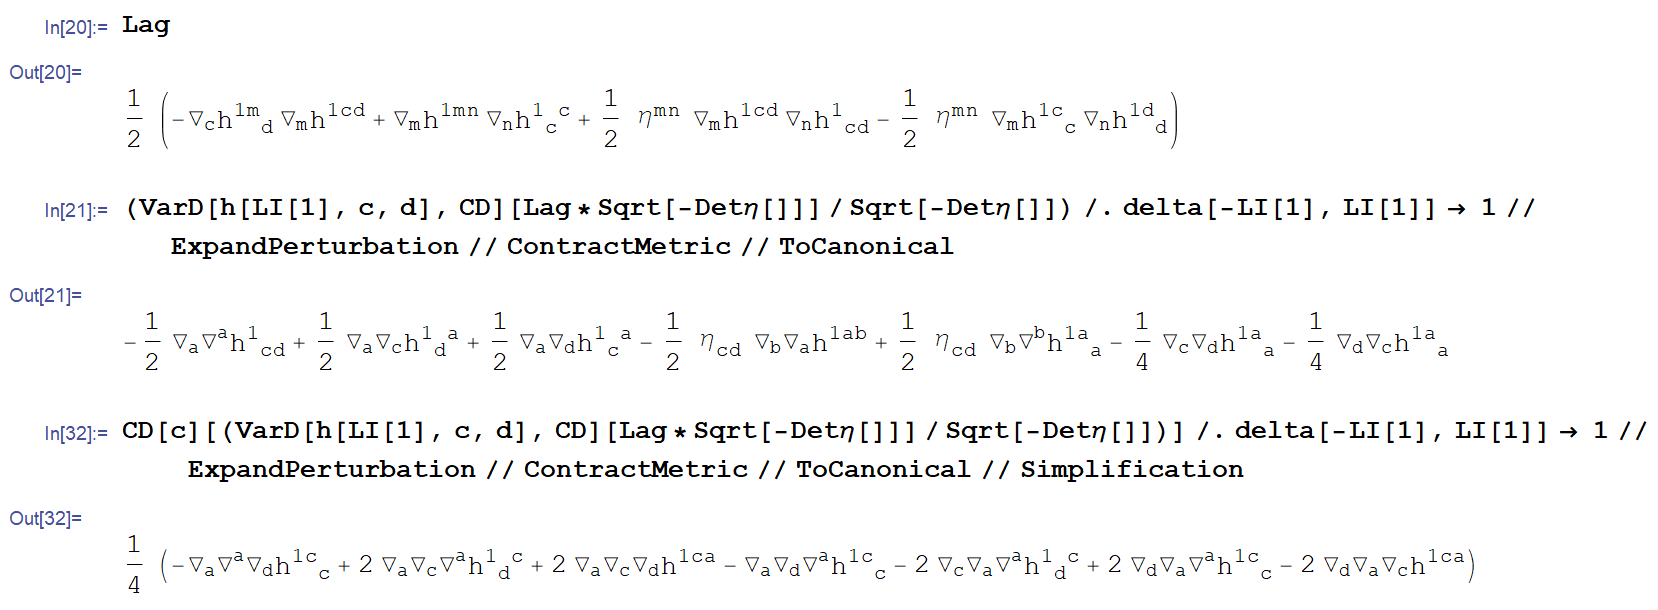
\includegraphics[scale=0.25]{CDG}
\end{figure}
So yes $\p^\mu G_{\mu\nu}$ is in fact identically zero. Thus, we must have that
\begin{align}\label{gauge-1}
\p^\mu \lc \f{1}{2}m^2 \lp h_{\mu\nu} - (1-a)\eta_{\mu\nu}h \rp \rc= 0 &\iff \boxed{\p^\mu h_{\mu\nu} - (1-a)\eta_{\mu\nu}\p^\mu h = 0}
\end{align}
Next, just like how we can write 
\begin{align}
A_\mu \sim \xi_\mu e^{ik\cdot x}
\end{align}
for the wave solution to the spin-1 field where $\xi_\mu$ is the polarization \textit{vector}, let us write
\begin{align}
h_{\mu\nu} \sim \xi_{\mu\nu}e^{ik\cdot x}
\end{align}
where $\xi_{\mu\nu}$ is the graviton's polarization tensor. With this we have
\begin{align}
\boxed{\xi_{\mu\nu}k^\mu - (1-a)\tensor{\xi}{^\mu_\mu}k_\nu = 0}
\end{align}
This is four equations for $\nu = 0,1,2,3$ which brings the number of degrees of freedom down from 10 to $10 - 4 = 6$ degrees of freedom. There is now one too many. How do we get rid of this? The answer lies in the factor $(1-a)$ and the contraction of $G^{\mu\nu}$.\\

Recall from \eqref{GGG} that
\begin{align}
G_{\mu\nu} = \f{1}{2}\lp -\square h_{\mu\nu} + \p_\sigma \p_\nu \tensor{h}{^\sigma_\mu}  
+ \p_\sigma \p_\mu \tensor{h}{^\sigma_\nu} 
- \eta_{\mu\nu}\p_\lambda \p_\sigma h^{\lambda\sigma} + \eta_{\mu\nu}\square h - \p_\mu\p_\nu h\rp,
\end{align}
which we have found by varying $\lag_{\text{linear}}$ in xACT with respect to $h_{\mu\nu}$. We wish to contract $G_{\mu\nu}$, with xACT as well:
\begin{lstlisting}
Lag := (1/
2)*((CD[-m][h[LI[1], m, n]])*(CD[-n][h[LI[1], -c, c]]) - (CD[-m][
h[LI[1], c, d]])*(CD[-c][h[LI[1], m, -d]]) + (1/2)*\[Eta][m, 
n]*(CD[-m][h[LI[1], c, d]])*(CD[-n][h[LI[1], -c, -d]]) - (1/
2)*\[Eta][m, 
n]*(CD[-m][h[LI[1], c, -c]])*(CD[-n][h[LI[1], d, -d]]))

(VarD[h[LI[1], c, d], CD][Lag*Sqrt[-Det\[Eta][]]]/
Sqrt[-Det\[Eta][]]) /. delta[-LI[1], LI[1]] -> 1 // 
ExpandPerturbation // ContractMetric // ToCanonical

\[Eta][c, 
d] (VarD[h[LI[1], c, d], CD][Lag*Sqrt[-Det\[Eta][]]]/
Sqrt[-Det\[Eta][]]) /. delta[-LI[1], LI[1]] -> 1 // 
ExpandPerturbation // ContractMetric // ToCanonical
\end{lstlisting}
\begin{figure}[!htb]
	\centering
	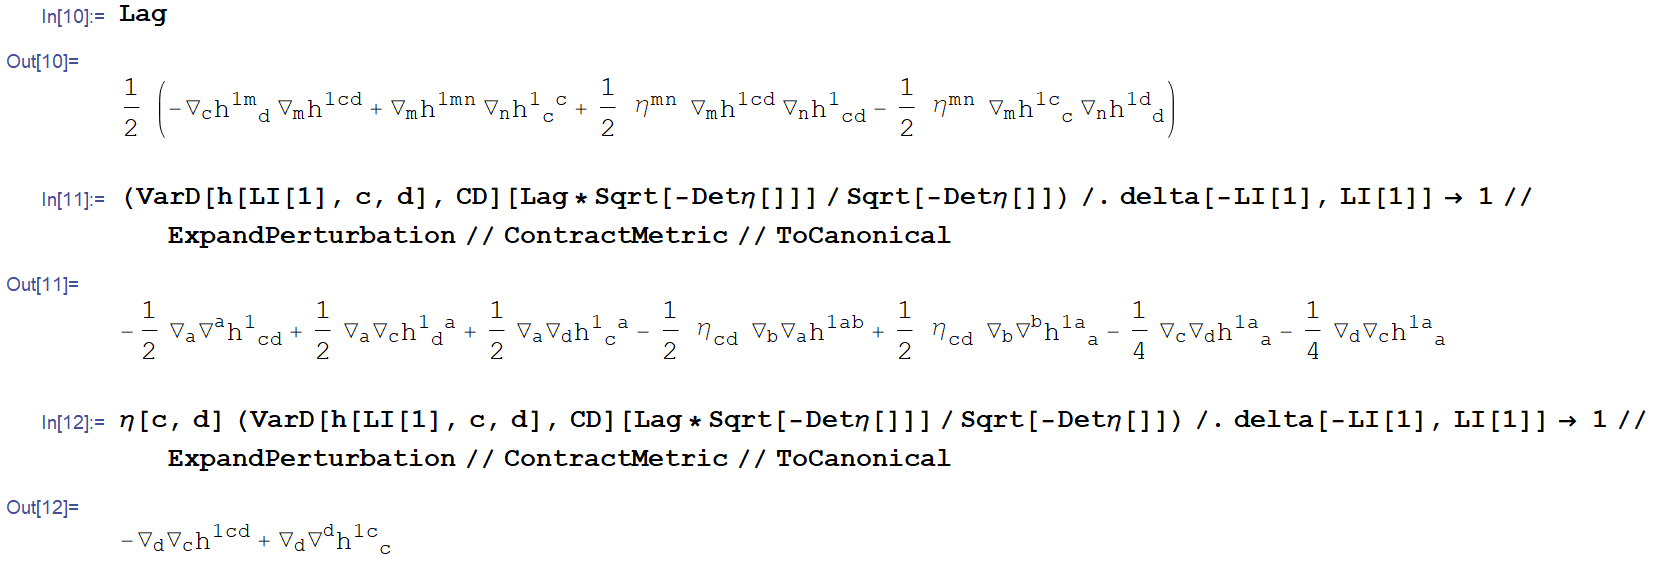
\includegraphics[scale=0.28]{Gcontract}
\end{figure}

This reads nicely as
\begin{align}\label{munuG}
\boxed{G=  \eta^{\mu\nu}G_{\mu\nu} = \p_\mu \p_\nu h^{\mu\nu} - \square h}
\end{align}
From the gauge fix in \eqref{gauge-fix}, we must have that
\begin{align}\label{munuH}
G = \eta^{\mu\nu}G_{\mu\nu} &= -\f{1}{2}m^2\eta^{\mu\nu}[ h_{\mu\nu} -(1-a)\eta_{\mu\nu}h ]\nn\\
&= -\f{1}{2}m^2 [h - 4(1-a)h]\nn\\
&= \boxed{\f{1}{2}m^2 (3 - 4a)h}
\end{align}
If we choose $a = 0$, then it follows from this equality that
\begin{align}
G =\f{1}{2}m^2h 
\end{align}
and from \eqref{gauge-1} that   
\begin{align}
\p^\mu h_{\mu\nu} - \p_\nu h = 0 \implies \p_\mu \p_\nu h^{\mu\nu} - \square h = 0.
\end{align}
But these combined give us $h = 0 \iff \tensor{h}{^\mu_\mu} \iff \tensor{\xi}{^\mu_\mu} = 0$. Aha! With the trace of $\xi_{\mu\nu}$ being zero, the number of polarizations is now $6-1 = 5$, as desired. This choice of the Fierz-Pauli tuning is now justified.\\



















\textit{Step 2.} Here we will show that when $a\neq 0$, the theory describes a massive spin 2 \textit{and} and a ghost scalar field with
\begin{align}
m_g^2  = -\f{3-4a}{2a}m^2.
\end{align}
Let us first show the motivation for defining the ghost scalar mass in this fashion. We have that \eqref{gauge-1} reads
\begin{align}
\p^\mu h_{\mu\nu} - (1-a)\eta_{\mu\nu}\p^\mu h = 0.
\end{align}
We wish to establish a relationship between $\square h$ and $\p^\mu \p^\nu h_{\mu\nu}$ for reasons we will see later. This means we should take $\p^\nu$ of the equation above. This gives
\begin{align}
\p^\nu \p^\mu h_{\mu\nu} - (1-a)\eta_{\mu\nu}\p^\nu \p^\mu h = 0.
\end{align}
But this equation simply screams
\begin{align}\label{just-then}
\p_\mu \p_\nu h^{\mu\nu} - (1-a)\square h = 0.
\end{align}

Nice! Now, from \eqref{munuG} and \eqref{munuH} we also know that
\begin{align}\label{just-now}
\p_\mu \p_\nu h^{\mu\nu} - \square h = -\f{1}{2}m^2(3-4a)h.
\end{align}
Therefore, we have from \eqref{just-now} and \eqref{just-then}
\begin{align}
-\f{1}{2}m^2 (3-4a) h + \square h = (1-a)\square h.
\end{align}
This simplifies to
\begin{align}
-\f{1}{2}m^2 (3-4a) h = -a\square h.
\end{align}
This equation is now begging to be put into Klein-Gordon form:
\begin{align}
\boxed{\lp -\f{1}{2a}m^2(3-4a) + \square \rp h = 0}
\end{align}
It only makes sense that we cast the mass term as $m_g^2$. And whatever this theory is, it is describing a massive scalar field with
\begin{align}
\boxed{m_g^2 = -\f{3-4a}{2a}m^2 }
\end{align}
Our next task is to show this is actually a ghost field. To this end, we invoke Hamiltonian analysis of Fierz-Pauli massive gravity with the $(1-a)$ coefficient. We first cast the Lagrangian 
\begin{align}
\lag = &-\f{1}{2}\p_\lambda h_{\mu\nu} \p^\lambda h^{\mu\nu} + \p_\mu h_{\nu\lambda}\p^\nu h^{\mu\lambda}\nn\\& - \p_\mu h^{\mu\nu}\p_\nu h + \f{1}{2}\p_\lambda h \p^\lambda h -\f{1}{2}m^2\lp h_{\mu\nu}h^{\mu\nu} - h^2 \rp
\end{align}
into Hamiltonian form. We start by Legendre transforming this Lagrangian only with respect to the spatial components of the perturbation metric, $h_{ij}$. The canonical momenta are defined as
\begin{align}
\pi_{ij} = \f{\p \lag}{\p \dot{h}_{ij}} \equiv \f{\p \lag}{\p (\p_0 h_{ij})}
\end{align}
where $\p$ is just the regular partial derivative. To evaluate this, we can expand out $\lag$ in terms of $\mu =0$ objects and $\mu = i = 1,2,3$ objects. If \href{https://digitalcommons.colby.edu/cgi/viewcontent.cgi?article=1721&context=honorstheses}{\underline{Greg Seyfarth}} is correct, then (deep breath now):
\begin{empheq}[box=\widefbox]{align*}
\lag = &\f{1}{2}(h_{jk,0})^2 + (h_{0k,j})^2 - \f{1}{2}(h_{jk,l})^2 - (h_{0k,j})(h_{0j,k}) - 2(h_{0j,k})(h_{jk,0})\nn\\
&+ (h_{kj,l})(h_{lj,k}) + (h_{0k,k})(h_{jj,0}) - \f{1}{2}(h_{jj,0})(h_{kk,0}) - (h_{00,l})(h_{jj,l})  \nn\\
&+\f{1}{2}(h_{jj,l})(h_{kk,l}) + (h_{0j,j})(h_{kk,0}) + (h_{jk,j})(h_{00,k}) - (h_{jk,j})(h_{ll,k}) \nn\\
& - \f{1}{2}m^2 \lb a h^2_{00} - 2h_{0j}^2 + h^2_{jk} + 2(1-a)h_{00}h_{ll} - (1-a)h^2_{ll} \rb.
\end{empheq}
To get these square terms in the Lagrangian it is necessary to integrate by parts and cancel like terms. I will not try to reproduce this since it is purely index manipulation.\\

Varying this Lagrangian gives equations of motions. Varying with respect to $h_{00}$ gives
\begin{align}
h_{jj,kk} - h_{jk,jk} - am^2h_{00} - m^2(1-a)h_{ll} - 0.
\end{align}
Varying with respect to $h_{0j}$ gives
\begin{align}
-h_{0j,kk} + h_{0k,jk} + h_{jk,0k} - h_{kk,0j} + m^2 h_{0j} = 0.
\end{align}
Varying with respect to $h_{jk}$ gives
\begin{align}
0= &\,\,\,h_{jk,00} - h_{jk,ll} - (h_{0j,0k} + h_{0k,0j}) + (h_{lk,lj} + h_{lj,lk})\nn\\
&\,\,\, + \delta_{jk}(2h_{0l,0l} - h_{ll,00} - h_{00,ll} + h_{mm,ll}- h_{lm,lm})\nn\\
&\,\,\,+ h_{00,jk} - h_{ll,jk} + m^2 h_{jk} + m^2(1-a)\delta_{jk}h_{00} - m^2(1-a)\delta_{jk}h_{ll}. 
\end{align}
With this, the Hamiltonian is
\begin{empheq}[box=\widefbox]{align*}
\ham &= \pi^{\mu\nu} h_{\mu\nu,0} - \lag \nn\\
&= \f{1}{2}(\pi_{jk})^2 - \f{1}{4}(\pi_{ll})^2 + 2 h_{0k,j}\pi_{jk} + \f{1}{2}(h_{jk,l})^2\nn\\
&\,\,\,\, -h_{jk,l}h_{lj,k} + h_{00,l}h_{kk,l} - \f{1}{2}h_{jj,l}h_{kk,l} - h_{jk,j}h_{00,k}+ h_{jk,j}h_{ll,k}\nn\\
&\,\,\,\, + \f{1}{2}m^2[ah^2_{00} - 2h^2_{0j} + h^2_{jk} + 2(1-a)h_{00}h_{ll}h - (1-a)h^2_{ll}].  
\end{empheq}
After a number of substitutions that I won't worry about too much here, the final form of the Hamiltonian is given by
\begin{empheq}[box=\widefbox]{align*}
\ham = &\f{1}{2}(\pi_{jk})^2 - \f{1}{4}(\pi_{ll})^2 + \f{1}{2}(\epsilon_{ijk} h_{kl,j})^2 -\f{1}{2}h_{jk,k}^2 + \f{1}{2}h^2_{jj,l} \nn\\
&\,\,\, + \f{1}{2}m^2[-ah^2 + h^2_{ll} + 2h_{0j}^2 + h^2_{jk}]
\end{empheq}
where $\epsilon_{ijk}$ is the Levi-Civita symbol.\\


The terms in the square brackets correspond to the Fierz-Pauli mass term in the original Lagrangian, while the rest of the terms come from the Lagrangian that gives the original Einstein tensor. We are interested in the square bracket terms when looking for ghosts in the theory. \\

When $a=0$, the square bracket becomes
\begin{align}
\f{1}{2}m^2[-ah^2 + h^2_{ll} + 2h_{0j}^2 + h^2_{jk}] \to \f{1}{2}m^2[h^2_{ll} + 2h_{0j}^2 + h^2_{jk}].
\end{align}
This term is positive-definite, which is good. But what about the other terms in the Hamiltonian? Well, we know that the rest of the Hamiltonian comes directly from the Lagrangian without the massive term. We also know that this piece of the theory is very well-behaved since we have a number of equations of motions and constraints to keep the degree of freedom correct. Thus, to see if the current theory contains ghost it suffices to look only at the massive term's contribution to the Hamiltonian. \\

Since we have already seen how $a= 0$ gives a well-behaved theory. Let's now consider $a\neq 0$. When $a\neq 0$, the modified Klein-Gordon equation looks like
\begin{align}
\lp -\f{3-4a}{2a}m^2 + \square\rp h = (\square + m_g^2)h = 0. 
\end{align}
Clearly the energy relation is 
\begin{align}
E^2 - p^2 = -m_g^2,
\end{align}
which has the wrong sign, i.e., the (ghostly) mass is imaginary. We might try to remedy this problem by requiring that
\begin{align}
\f{3-4a}{2a} > 0 \iff 0 < a < \f{3}{4}.
\end{align}
But this ensures that the coefficient of $h^2$ in the term
\begin{align}
\f{1}{2}m^2[-ah^2 + h^2_{ll} + 2h_{0j}^2 + h^2_{jk}]
\end{align}
is always negative, rendering the Hamiltonian non-positive-definite. We also can't constrain $h$ in order to bring the degree of freedom down from 6 to 5. This means that when $a\neq 0$ we have (1) an imaginary mass, (2) non-positive definite Hamiltonian, and (3) and extra degree of freedom in the theory. This creates a ghost mode in the theory.\\ \qed

With that we have showed how the tuning $a = 0$ is justified, and how a massive scalar ghost mode appears (with negative kinetic energy) in the theory when $a \neq 0$. As a little aside, when $a\neq0$ and $a$ is small, the mass $m_g^2$ goes like $\sim 1/a$. This goes to infinity as the Fierz-Pauli tuning is approached, rendering it non-dynamical.


























\subsubsection{Free solutions and Graviton mode functions}

In this section we find the space of equations of motion, i.e. solutions to $\delta S = 0$. We will then show that it transforms as a massive spin 2 representation of the Lorentz group, i.e. showing that the action propagates precisely one massive graviton (we will understand what this means later). To this end, we consider the Fierz-Pauli action with the correct Fierz-Pauli tuning:
\begin{align}
S_{FP} = \int d^Dx\, &-\f{1}{2}\p_\lambda h_{\mu\nu} \p^\lambda h^{\mu\nu} + \p_\mu h_{\nu\lambda}\p^\nu h^{\mu\lambda}\nn\\& - \p_\mu h^{\mu\nu}\p_\nu h + \f{1}{2}\p_\lambda h \p^\lambda h -\f{1}{2}m^2\lp h_{\mu\nu}h^{\mu\nu} - h^2 \rp.
\end{align}  
Setting $\delta S = 0 \iff \delta \lag / \delta h^{\mu\nu} = 0$, i.e., the variational derivative of the integrand with respect to the inverse metric perturbation $h^{\mu\nu}$ is zero. We can readily to this in xACT:
\begin{lstlisting}
LagFP := -((CD[-m][h[LI[1], m, n]])*(CD[-n][
h[LI[1], -c, c]]) - (CD[-m][h[LI[1], c, d]])*(CD[-c][
h[LI[1], m, -d]]) + (1/2)*\[Eta][m, 
n]*(CD[-m][h[LI[1], c, d]])*(CD[-n][h[LI[1], -c, -d]]) - (1/
2)*\[Eta][m, 
n]*(CD[-m][h[LI[1], c, -c]])*(CD[-n][h[LI[1], d, -d]])) - (1/
2)*M^2*(h[LI[1], m, n]*
h[LI[1], -m, -n] - (1 - 0) h[LI[1], c, -c]*h[LI[1], d, -d])

(VarD[h[LI[1], c, d], CD][LagFP*Sqrt[-Det\[Eta][]]]/
Sqrt[-Det\[Eta][]]) == 0 /. delta[-LI[1], LI[1]] -> 1 // 
ExpandPerturbation // ContractMetric // ToCanonical
\end{lstlisting}
to get
\begin{figure}[!htb]
	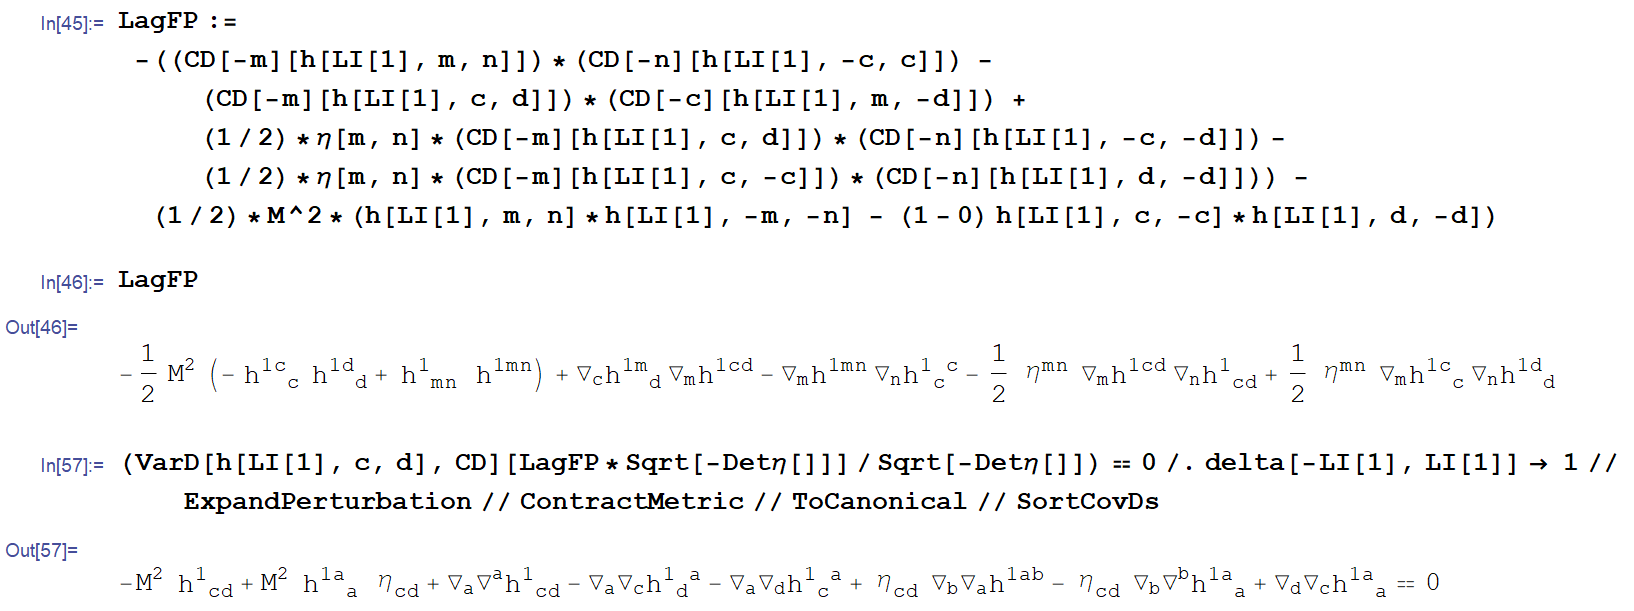
\includegraphics[scale=0.26]{free-soln}
\end{figure}\\
which says
\begin{align}
\f{\delta \lag}{\delta h^{\mu\nu}} &= \square h_{\mu\nu} - \p_\lambda \p_\mu \tensor{h}{^\lambda_\nu} - \p_\lambda \p_\nu \tensor{h}{^\lambda_\mu} + \eta_{\mu\nu}\p_\lambda \p_\sigma h^{\lambda\sigma} + \p_\mu \p_\nu h - \eta_{\mu\nu}\square h  \nn\\
&\,\,\,\,\,- m^2(h_{\mu\nu} - \eta_{\mu\nu}h)\nn\\
&= 0.
\end{align}

Okay, to get what constraints this equation gives us we first let $\p^\mu$ act on this equation:
\begin{lstlisting}
CD[c][(VarD[h[LI[1], c, d], CD][LagFP*Sqrt[-Det\[Eta][]]]/
Sqrt[-Det\[Eta][]])] /. delta[-LI[1], LI[1]] -> 1 // 
ExpandPerturbation // ContractMetric // 
ToCanonical // Simplification
\end{lstlisting}
\begin{figure}[!htb]
	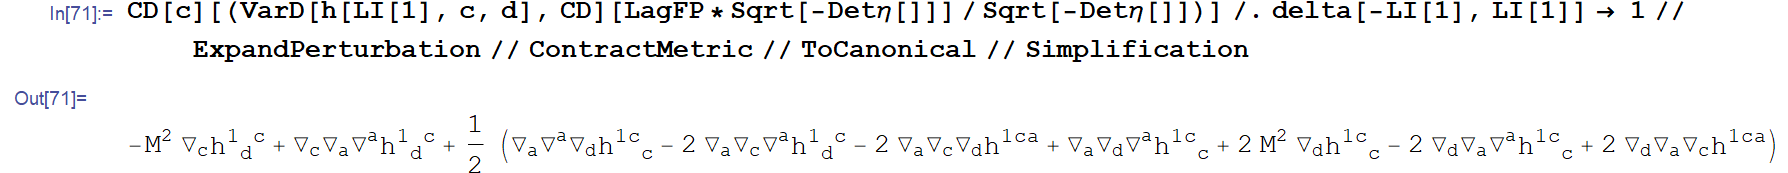
\includegraphics[scale=0.26]{covD}
\end{figure}
Looking at this expression (which equals 0) for a while we can see that all terms without the $m^2$ factor cancel, which makes sense because $\p^\mu G_{\mu\nu} = 0$ where $G^{\mu\nu}$ is the Einstein tensor in the massless case. This expression then just simplify to
\begin{align}
\boxed{\p^\mu h_{\mu\nu} - \p_\nu h = 0 \iff \p_\mu h^{\mu\nu} - \p^\nu h = 0}
\end{align}
Plugging this back into the equation of motion, we find
\begin{align}
0 &= \square h_{\mu\nu} - \p_\lambda \p_\mu \tensor{h}{^\lambda_\nu} - \p_\lambda \p_\nu \tensor{h}{^\lambda_\mu} + \eta_{\mu\nu}\p_\lambda \p_\sigma h^{\lambda\sigma} + \p_\mu \p_\nu h - \eta_{\mu\nu}\square h - m^2(h_{\mu\nu} - \eta_{\mu\nu}h)\nn\\
&= \square h_{\mu\nu} - \p_\mu \p^\lambda h_{\lambda\nu} - \p_\nu \p^\lambda h_{\lambda\mu} + \eta_{\mu\nu}\p_\lambda \p^\lambda h + \p_\mu \p_\nu h - \eta_{\mu\nu}\square h - m^2(h_{\mu\nu} - \eta_{\mu\nu}h)\nn\\
&= \square h_{\mu\nu} - \p_\mu \p_\nu h - \p_\nu \p_\mu h + \cancel{\eta_{\mu\nu}\square h} + \p_\mu \p_\nu h - \cancel{\eta_{\mu\nu}\square h} - m^2(h_{\mu\nu} - \eta_{\mu\nu}h)\nn\\
&= \square h_{\mu\nu} - \p_\mu \p_\nu h - m^2(h_{\mu\nu} - \eta_{\mu\nu}h).
\end{align}
So we have
\begin{align}
\boxed{\square h_{\mu\nu} - \p_\mu \p_\nu h - m^2(h_{\mu\nu} - \eta_{\mu\nu}h) = 0}
\end{align}
Contracting we find that $\boxed{h=0}$
\begin{align}
0 &= \eta^{\mu\nu}\lp \square h_{\mu\nu} - \p_\mu \p_\nu h - m^2(h_{\mu\nu} - \eta_{\mu\nu}h) \rp\nn\\
&= \square h - \square h - m^2(h - 4h) \iff h = 0.
\end{align}
But this just says
\begin{align}
\p^\mu h_{\mu\nu} = \p_\nu h = 0 \implies (\square - m^2)h_{\mu\nu} = 0.
\end{align}
And so just to summarize, we have
\begin{align}
\boxed{(\square - m^2)h_{\mu\nu} = 0; \quad \p^\mu h_{\mu\nu} = 0; \quad h = 0}
\end{align}
It turns out that these three equations and the original equation of motion $\delta \lag = 0$ are equivalent statements. However, when put into this form (involving three simple equations), degree-of-freedom-counting is much easier. For $D = 4$, the first equation describe the evolution for a ten-component symmetric tensor $h$. The second equation reduces 4 more d.o.f. The last equation sets the trace, hence killing the last d.o.f, making $h_{\mu\nu}$ have only 5 d.o.f. In total, we are left with the 5 real space d.o.f of a 4-dimensional spin 2 particle ($5 = 2s+1 = 2\times 2 + 1$). \\

Next, we wish to solve for $h_{\mu\nu}$ firstly from the Klein-Gordon equation. This turns out to be a reasonably easy differential equation whose general solution has the form
\begin{align}
\boxed{h^{\mu\nu}(x) = \int \f{d^d\mathbf{p}}{\sqrt{(2\pi)^d 2\omega_\mathbf{p}}} \lb h^{\mu\nu}(\mathbf{p})e^{ip\cdot x} + {h^{\mu\nu}}^*(\mathbf{p})e^{-ip\cdot x}\rb}
\end{align}  
Here $\mathbf{p}$ are the spatial momenta:
\begin{align}
\omega_\mathbf{p} = \sqrt{\mathbf{p}^2 +m^2},
\end{align}
and the $D$ momenta $p^\mu$ are on shell so that $p^\mu =(\omega_\mathbf{p}, \mathbf{p})$. We then express the Fourier coefficients $h^{\mu\nu}(\mathbf{p})$ in terms of basis symmetric tensors indexed by $\lambda$:
\begin{align}
h^{\mu\nu}(\mathbf{p}) = a_{\mathbf{p},\lambda}\bar{\mathbf{\epsilon}}^{\mu\nu}(\mathbf{p},\lambda)
\end{align}
where
\begin{align}
\bar{\mathbf{\epsilon}}^{\mu\nu}(\mathbf{p},\lambda) = L^\mu_\alpha(p)L^\nu_\beta(p)\bar{\mathbf{\epsilon}}^{\alpha\beta}(\mathbf{k},\lambda).
\end{align}
Here $L^\mu_\alpha(p)$ are boosts of the form
\begin{align}
&L^i_j(p) = \delta^i_j + \f{1}{\abs{\mathbf{p}}^2}(\gamma - 1)\mathbf{p}^i\mathbf{p}^j\nn\\
&L^i_0(p) = L^0_i(\mathbf{p}) = \f{\mathbf{p}^i}{\abs{\mathbf{p}}}\sqrt{\gamma^2 - 1}\nn\\
&L^0_0(p) = \gamma = \f{p^0}{m}  = \sqrt{\abs{p}^2 + \f{m^2}{m}}
\end{align}
such that the momentum $k$ is taken from $k^\mu = (m,0,0,0)$ to $p$ where $p^\mu = L^\mu_\alpha(p) k^\alpha$. This stand boost choose for us the basis at $\mathbf{p}$, relative to that at $\mathbf{k}$. \\

With $\p_\mu h^{\mu\nu} = (\p/\p x^\mu)h^{\mu\nu}  = 0$ we have
\begin{align}
0 &= \p_\mu \lc \int \f{d^d\mathbf{p}}{\sqrt{(2\pi)^d 2\omega_\mathbf{p}}} \lb h^{\mu\nu}(\mathbf{p})e^{ip\cdot x} + {h^{\mu\nu}}^*(\mathbf{p})e^{-ip\cdot x}\rb  \rc\nn\\
&= \int \f{d^d\mathbf{p}}{\sqrt{(2\pi)^d 2\omega_\mathbf{p}}}
\lb ip_\mu  h^{\mu\nu}(\mathbf{p})e^{ip_\mu x^\mu} + h.c. \rb\nn\\
&\implies p_\mu h^{\mu\nu}(\mathbf{p}) = 0\nn\\
&\implies L^\sigma_\mu(p)k_\sigma \lp a_{\mathbf{p},\lambda}\bar{\mathbf{\epsilon}}^{\mu\nu}(\mathbf{p},\lambda)\rp = 0\nn\\
&\implies k_\sigma L^\sigma_\mu(p)L^\mu_\alpha(p)L^\nu_\beta(p)\bar{\mathbf{\epsilon}}^{\alpha\beta}(\mathbf{k},\lambda) =0 \nn\\
&\implies k_\sigma \delta^\sigma_\alpha(p)L^\nu_\beta(p)\bar{\mathbf{\epsilon}}^{\alpha\beta}(\mathbf{k},\lambda) =0 \nn\\
&\implies k_\alpha L^\nu_\beta(p)\bar{\mathbf{\epsilon}}^{\alpha\beta}(\mathbf{k},\lambda) =0 \nn\\
&\implies k_\alpha\bar{\mathbf{\epsilon}}^{\alpha\beta}(\mathbf{k},\lambda) =0 \nn\\
&\implies \boxed{k_\mu \bar{\mathbf{\epsilon}}^{\mu\nu}(\mathbf{k},\lambda) = 0  }
\end{align} 
We also have the condition $h=0$, which implies
\begin{align}
0 &= \eta_{\mu\nu}\int \f{d^d\mathbf{p}}{\sqrt{(2\pi)^d 2\omega_\mathbf{p}}} \lb h^{\mu\nu}(\mathbf{p})e^{ip\cdot x} + {h^{\mu\nu}}^*(\mathbf{p})e^{-ip\cdot x}\rb\nn\\
&\implies \eta_{\mu\nu}a_{\mathbf{p},\lambda}\bar{\mathbf{\epsilon}}^{\mu\nu}(\mathbf{p},\lambda) = 0\nn\\
&\implies \eta_{\mu\nu}a_{\mathbf{p},\lambda}L^\mu_\alpha(p)L^\nu_\beta(p)\bar{\mathbf{\epsilon}}^{\alpha\beta}(\mathbf{k},\lambda) = 0\nn\\
&\implies \dots (\text{requires writing out when $\alpha=\mu$, $\beta=\nu$, etc.})\nn\\
&\implies \boxed{\eta_{\mu\nu}\bar{\mathbf{\epsilon}}^{\mu\nu}(\mathbf{k},\lambda) = 0}
\end{align}
These two conditions imply that $\bar{\mathbf{\epsilon}}^{\mu\nu}(\mathbf{k},\lambda)$ is purely spatial, i.e.
\begin{align}
\boxed{\bar{\epsilon}^{0\mu}(\mathbf{k},\lambda) = \bar{\epsilon}^{0\mu}(\mathbf{k},\lambda)   = 0}
\end{align}
i.e.,
\begin{align}
[\bar{\mathbf{\epsilon}}^{\mu\nu}] = \begin{pmatrix}
0 &0&0&0\\
0&\bar{\mathbf{\epsilon}}^{11}&\bar{\mathbf{\epsilon}}^{12}&\bar{\mathbf{\epsilon}}^{13}\\
0&\bar{\mathbf{\epsilon}}^{12}&\bar{\mathbf{\epsilon}}^{22}&\bar{\mathbf{\epsilon}}^{23}\\
0&\bar{\mathbf{\epsilon}}^{13}&\bar{\mathbf{\epsilon}}^{23}&\bar{\mathbf{\epsilon}}^{33}\\
\end{pmatrix}
\end{align}
and that $\bar{\mathbf{\epsilon}}^{\mu\nu}(\mathbf{k},\lambda)$ is traceless, i.e.,
\begin{align}
\boxed{\bar{\mathbf{\epsilon}}^i_i(\mathbf{k},\lambda) = 0}
\end{align}
Hence, this basis is a collection of $d(d+1)/2$ symmetric, traceless spatial tensors with index $\lambda = 1,\dots,d(d+1)/2$. \\

We demand further that this is an orthonormal basis:
\begin{align}
\boxed{\bar{\mathbf{\epsilon}}^{\mu\nu}(\mathbf{k},\lambda)\bar{\mathbf{\epsilon}}^*_{\mu\nu}(\mathbf{k},\lambda') = \delta_{\lambda\lambda'}}
\end{align}


\textit{(some things about group theory here... in order to make conditions work for $\mathbf{p}$ and not $\mathbf{k}$..., i.e.,}
\begin{align}
\boxed{p_\mu \mathbf{\epsilon}^{\mu\nu}(\mathbf{p},\lambda) = 0; \quad \eta_{\mu\nu}\mathbf{\epsilon}^{\mu\nu}(\mathbf{p},\lambda) = 0}
\end{align}

\textit{I will get back to this later)}\\

In any case, the general solution $h^{\mu\nu}(x)$ can now be written in term of the new $\mathbf{p}$-dependent basis:
\begin{align}
h^{\mu\nu}(x) = \int \f{d^d\mathbf{p}}{\sqrt{(2\pi)^d 2\omega_\mathbf{p}}} \sum_\lambda a_{\mathbf{p},\lambda} \mathbf{\epsilon}^{\mu\nu}(\mathbf{p},\lambda)e^{ip\cdot x} + a^*_{\mathbf{p},\lambda} \mathbf{\epsilon}^{*\mu\nu}(\mathbf{p},\lambda)e^{-ip\cdot x}
\end{align}
























\subsubsection{The Propagator}

There is a treatment of the F-P propagator in A. Zee's book which I have reproduced in one of sections in \textit{Gravity as Field Theory}. But in any case, I will reproduce the derivation here (plus some details) following Hinterbichler's paper. \\

The recall the full Fierz-Pauli action:
\begin{empheq}[box=\widefbox]{align}
S_{FP} = \int d^Dx\, &-\f{1}{2}\p_\lambda h_{\mu\nu} \p^\lambda h^{\mu\nu} + \p_\mu h_{\nu\lambda}\p^\nu h^{\mu\lambda}\nn\\& - \p_\mu h^{\mu\nu}\p_\nu h + \f{1}{2}\p_\lambda h \p^\lambda h -\f{1}{2}m^2\lp h_{\mu\nu}h^{\mu\nu} - h^2 \rp
\end{empheq}
We wish to write this action in the form
\begin{align}
S = \int d^Dx\,\f{1}{2}h_{\mu\nu}\mathcal{O}^{\mu\nu,\alpha\beta}h_{\alpha\beta}
\end{align}
so as to resemble quantum field theory where the action appearing in the generating function 
\begin{align}
\Z = \zeta \int \mathfrak{D}[\phi] e^{i\int d^4x \lag[\phi]}\sim e^{\f{-i}{2}JA^{-1}J} \equiv e^{\f{-i}{2}\iint d^4xd^4y J(x)\D(x-y)J(y)}
\end{align}
where $J(\cdot)$ is the source and $\D(x-y) \equiv A^{-1}$ is the propagator and $A$ is the original differential operator in the Lagrangian. By analogy, the graviton propagator $\D_{\alpha\beta,\mu\nu}$ is defined to be the inverse of the second-order differential operator $\mathcal{O}^{\mu\nu,\alpha\beta}$. The goal of this section is to obtain an expression for $\D_{\alpha\beta,\mu\nu}$.\\

We wish to turn $S_{FP}$ into the form involving $\mathcal{O}^{\mu\nu,\alpha\beta}$ where $\mathcal{O}^{\mu\nu,\alpha\beta}$ is some operator. The comma here doesn't mean (covariant) derivatives of any kind. It is there just to remind us that $\mu\nu$ and $\alpha\beta$ can be treated as two (pair of) indices. To write the action this way we are required to integrate the integrand of $S_{FP}$ by parts so that every term in the resulting integrand looks like $h_{\mu\nu}\diamondsuit^{\mu\nu,\alpha\beta}h_{\alpha\beta}$ where $\diamondsuit^{\mu\nu,\alpha\beta}$ is some operator. There are five terms so let's hope things don't get out of hand (they don't). The first term can be re-written as
\begin{align}
\int d^Dx\, \f{1}{2} \lp -\p_\lambda h_{\mu\nu}\p^\lambda h^{\mu\nu} \rp 
&= \int d^Dx\, \f{1}{2}\lp h_{\mu\nu} \square \eta^{\mu\alpha}\eta^{\nu\beta}h_{\alpha\beta} \rp\nn\\
&= \int d^Dx\, \f{1}{2}\lp h_{\mu\nu} \square \tensor{\eta}{^{(\mu}_\alpha}\tensor{\eta}{^{\nu)}_{\beta}}h^{\alpha\beta} \rp
\end{align}
where the little brackets denote the symmetry in $\mu \leftrightarrow \nu$, meaning that we can swap $\mu$ and $\nu$ as we please. \\

The second term is the trickiest:
\begin{align}
\int d^Dx\, \lp\p_\mu h_{\nu\lambda}\p^\nu h^{\mu\lambda}\rp &= \int d^Dx\, \lp - h_{\nu\lambda}\p_\mu \p^\nu h^{\mu\lambda}\rp \nn\\
&= \int d^Dx\, \lp -h_{\mu\nu}\p^\alpha \p^\mu \eta^{\nu\beta}h_{\alpha\beta} \rp\nn\\
&= \int d^Dx\, \lb h_{\mu\nu}\lp - \p^\mu \p^\alpha \eta^{\nu\beta} - \p^\nu \p^\beta \eta^{\mu\alpha} + \p^\alpha \p^\beta \eta^{\mu\nu}  \rp h_{\alpha\beta} \rb\nn\\
&= \int d^Dx\, \lb h_{\mu\nu} \lp -2\p^{(\mu} \p^{(\alpha} \tensor{\eta}{^{\nu)\beta)}} + \p^\alpha \p^\beta \eta^{\mu\nu}  \rp h_{\alpha\beta} \rb\nn\\
&= \int d^Dx\, \lb h_{\mu\nu} \lp -2\p^{(\mu} \p_{(\alpha} \tensor{\eta}{^{\nu)}_{\beta)}} + \p_\alpha \p_\beta \eta^{\mu\nu}  \rp h^{\alpha\beta} \rb,
\end{align}
where we're treating $\mu$ and $\nu$ are one pair and $\alpha$ and $\beta$ as another pair. The last three terms are quite easy:
\begin{align}
\int d^Dx\, \lp-\p_\mu h^{\mu\nu}\p_\nu h \rp 
&= \int d^Dx\, \lp h^{\mu\nu}\p_\mu\p_\nu h \rp  \nn\\
&= \int d^Dx\, \lp h_{\mu\nu}\p^\mu\p^\nu \eta^{\alpha\beta}h_{\alpha\beta} \rp  \nn\\
&= \int d^Dx\, \lp h_{\mu\nu}\p^\mu\p^\nu \eta_{\alpha\beta}h^{\alpha\beta} \rp.
\end{align}
\begin{align}
\int d^Dx\, \f{1}{2}\lp \p_\lambda h \p^\lambda h \rp
&= \int d^Dx\, \f{1}{2}\lp \p_\lambda h \p^\lambda h \rp\nn\\ 
&= \int d^Dx\, \f{1}{2}\lp -h\square h \rp\nn\\
&= \int d^Dx\, \f{1}{2}\lp -h_{\mu\nu}\square \eta^{\mu\nu}\eta^{\alpha\beta}h_{\alpha\beta} \rp\nn\\
&= \int d^Dx\, \f{1}{2}\lp -h_{\mu\nu}\square \eta^{\mu\nu}\eta_{\alpha\beta}h^{\alpha\beta} \rp.
\end{align}
\begin{align}
\int d^Dx\, -\f{m^2}{2}\lp h_{\mu\nu}h^{\mu\nu} - h^2 \rp
&= \int d^Dx\, \f{-m^2}{2}\lp h_{\mu\nu}h^{\mu\nu} - h^2 \rp\nn\\
&= \int d^Dx\, \f{-m^2}{2}\lb h_{\mu\nu}\lp\eta^{\mu\alpha}\eta^{\nu\beta}  - \eta^{\mu\nu}\eta^{\alpha\beta}\rp h_{\alpha\beta}  \rb \nn\\
&= \int d^Dx\, \f{-m^2}{2}\lb h_{\mu\nu}\lp\eta^{\mu\alpha}\eta^{\nu\beta}  - \eta^{\mu\nu}\eta^{\alpha\beta}\rp h_{\alpha\beta}  \rb \nn\\
&= \int d^Dx\, \f{-m^2}{2}\lb h_{\mu\nu}\lp\tensor{\eta}{^{(\mu}_\alpha}\tensor{\eta}{^{\nu)}_\beta}  - \eta^{\mu\nu}\eta_{\alpha\beta}\rp h^{\alpha\beta}  \rb.
\end{align}
Putting everything together we have
\begin{align}
\boxed{\tensor{\mathcal{O}}{^{\mu\nu}_{\alpha\beta}} = \lp \tensor{\eta}{^{(\mu}_\alpha}\tensor{\eta}{^{\nu)}_\beta}  - \eta^{\mu\nu}\eta_{\alpha\beta} \rp (\square - m^2) -2\p^{(\mu} \p_{(\alpha} \tensor{\eta}{^{\nu)}_{\beta)}} + \p_\alpha \p_\beta \eta^{\mu\nu} + \p^\mu\p^\nu \eta_{\alpha\beta}}
\end{align}


This operator $\mathcal{O}$ is a second order differential operator. By the symmetry in the index-pairs: $\mu\nu$ and $\alpha\beta$, we have the following property:
\begin{align}
\mathcal{O}^{\mu\nu,\alpha\beta} = \mathcal{O}^{\nu\mu,\alpha\beta} = \mathcal{O}^{\mu\nu,\beta\alpha} = \mathcal{O}^{\nu\mu,\beta\alpha}.
\end{align}
There's nothing surprising about this. It is just a fact that might be useful later. \\

With this operator, the equation of motion can now be written succinctly as
\begin{align}
\boxed{\f{\delta \lag}{\delta h_{\mu\nu}} = \mathcal{O}^{\mu\nu,\alpha\beta}h_{\alpha\beta}= 0} 
\end{align}

Recall in QFT where the propagator $\D$ is defined as the inverse of the differential operator $A$, we do the same thing here and define the propagator $\D_{\alpha\beta,\sigma\lambda}$ as the inverse of $\mathcal{O}^{\mu\nu,\alpha\beta}$:
\begin{align}
\boxed{\mathcal{O}^{\mu\nu,\alpha\beta}\D_{\alpha\beta,\sigma\lambda} = \f{i}{2}\lp \delta^\mu_\sigma \delta^\nu_\lambda + \delta^\nu_\sigma\delta^\mu_\lambda \rp}
\end{align}
which obeys the same index symmetries as $\mathcal{O}$.\\

To derive an expression for $\D$, we first write $\mathcal{O}$ in momentum space:
\begin{align}
\tensor{\mathcal{O}}{^{\mu\nu}_{\alpha\beta}}(\p \to ip) = &-\lp \tensor{\eta}{^{(\mu}_\alpha}\tensor{\eta}{^{\nu)}_\beta}  - \eta^{\mu\nu}\eta_{\alpha\beta} \rp (p^2 + m^2)\nn\\
&+2p^{(\mu} p_{(\alpha} \tensor{\eta}{^{\nu)}_{\beta)}} - p_\alpha p_\beta \eta^{\mu\nu} - p^\mu p^\nu \eta_{\alpha\beta}
\end{align}
where $\p \to ip$ denotes replacing $\p$ by $ip$ when we go to momentum space. \\

Upon inspection, we can solve for $\D$ and find
\begin{align}
\boxed{\D_{\alpha\beta,\sigma\lambda} = \f{-i}{p^2 +m^2}\lb \f{1}{2}\lp P_{\alpha\sigma}P_{\beta\lambda} + P_{\alpha\lambda}P_{\beta\sigma} \rp - \f{1}{D-1}P_{\alpha\beta}P_{\sigma\lambda} \rb}
\end{align}
where
\begin{align}
P_{\alpha\beta} = \eta_{\alpha\beta} + \f{p_\alpha p_\beta}{m^2}.
\end{align}
I won't into the details about how we can obtain this. I will just say that we can readily verify that $\D$ is indeed the inverse of the $\mathcal{O}$, in momentum space. \\

When the momentum is large, the propagator behaves as $\sim p^2 / m^4$ (rather than $1/p^2$ in the meson theory, say), and so we can't verify if the theory is renormalizable or not using the conventional power counting method. We will see later how to overcome this difficulty by rewriting the theory in a way in which all propagators go similar to $\sim 1/p^2$ at high energy.   \\

We might learn something from comparing this propagator to the propagator in the $m=0$ case. In the $m=0$ case, the action can be written as
\begin{align}
S_{m=0} = \int d^Dx\, \f{1}{2}h_{\mu\nu}\mathcal{E}^{\mu\nu,\alpha\beta}h_{\al\be}
\end{align} 
where now the differential operator $\mathcal{E}$ is just the operator $\mathcal{O}$ evaluated at $m=0$:
\begin{align}
\tensor{\mathcal{E}}{^{\mu\nu}_{\alpha\beta}} &= \tensor{\mathcal{O}}{^{\mu\nu}_{\alpha\beta}}({m=0})\nn\\
&=  \lp \tensor{\eta}{^{(\mu}_\alpha}\tensor{\eta}{^{\nu)}_\beta}  - \eta^{\mu\nu}\eta_{\alpha\beta} \rp \square -2\p^{(\mu} \p_{(\alpha} \tensor{\eta}{^{\nu)}_{\beta)}} + \p_\alpha \p_\beta \eta^{\mu\nu} + \p^\mu\p^\nu \eta_{\alpha\beta}
\end{align}
This propagator also inherits the usual index symmetry: $\mu \leftrightarrow \nu$ and $\alpha \leftrightarrow \beta$. Letting $\mathcal{E}$ act on some symmetric tensor $Z_{\alpha\beta}$ we find
\begin{align}
\mathcal{E}^{\mu\nu,\alpha\beta}Z_{\alpha\beta} &= \tensor{\mathcal{E}}{^{\mu\nu}_{\alpha\beta}}Z^{\alpha\beta}\nn\\
&= \lc\lp \tensor{\eta}{^{(\mu}_\alpha}\tensor{\eta}{^{\nu)}_\beta}  - \eta^{\mu\nu}\eta_{\alpha\beta} \rp \square -2\p^{(\mu} \p_{(\alpha} \tensor{\eta}{^{\nu)}_{\beta)}} + \p_\alpha \p_\beta \eta^{\mu\nu} + \p^\mu\p^\nu \eta_{\alpha\beta}\rc Z^{\alpha\beta}\nn\\
&= \square Z^{\mu\nu} - \eta^{\mu\nu}\square Z -2\p^{(\mu} \p_{(\alpha} \tensor{\eta}{^{\nu)}_{\beta)}}Z^{\alpha\beta} + \p^\mu\p^\nu Z + \eta^{\mu\nu}\p_\alpha\p_\beta Z^{\alpha\beta}\nn\\
&= \square Z^{\mu\nu} - \eta^{\mu\nu}\square Z -2\p^{(\mu} \p_{\alpha} \tensor{Z}{^{\nu)\alpha}} + \p^\mu\p^\nu Z + \eta^{\mu\nu}\p_\alpha\p_\beta Z^{\alpha\beta}.
\end{align}

Now, recall that the $m=0$ action has the gauge symmetry
\begin{align}
\delta h_{\mu\nu} = \p_\mu \epsilon_\nu + \p_\nu \epsilon_\mu
\end{align}
which is broken when $m\neq 0$, which implies that the operator $\mathcal{E}$ is not invertible (has non-trivial kernel, i.e. there are distinct solutions to the same problem). In order to find the propagator (of equivalently the inverse of the differential operator), we must impose a gauge. We in fact have seen this gauge before in Zee's and Sean Carroll's treatment of massive gravity. The necessary gauge condition is called the harmonic gauge or de Donder gauge or Lorenz gauge:
\begin{align}
\p^\mu h_{\mu\nu} - \f{1}{2}\p_\nu h = 0.
\end{align}   
We also know that in this gauge the equation of motion reads
\begin{align}\label{no-source}
\square h_{\mu\nu} - \f{1}{2}\eta_{\mu\nu}\square h  =0.
\end{align}
The Lagrangian associated with this gauge condition has an additive gauge-fixing term
\begin{align}
\lag_{GF} = -\lp \p^\nu h_{\mu\nu} - \f{1}{2}\p_\mu h \rp^2,
\end{align}
which we also have seen in Zee's treatment. This term actually follows from the Faddeev-Popov gauge fixing process, but I won't go into too much detail here (for reference, please refer to \textit{Gravity as a Field Theory} in one of the earlier sections). \\

When we write the gauge-fixed action as
\begin{align}
S = \int d^Dx\, (\lag + \lag_{GF}) = \int d^Dx\, \f{1}{2}h_{\mu\nu}\tilde{\mathcal{O}}^{\mu\nu,\alpha\beta}h_{\alpha\beta}
\end{align}
where, from our results in \textit{Gravity and Beyond}
\begin{align}
\lag + \lag_{GF} &= -\f{1}{2}\p_\lambda h^{\mu\nu}\p^\lambda h_{\mu\nu} +\f{1}{4} \p_\lambda \tensor{h}{^\mu_\mu} \p^\lambda \tensor{h}{^\nu_\nu} \nn\\
&= \f{1}{2}h_{\mu\nu}\square h^{\mu\nu} - \f{1}{4}h\square h
\end{align}
where some slight discrepancies in the signs of the Lagrangian here and in the earlier sections arise due to whether we vary $\lag$ with respect to  $h_{\mu\nu}$ or $h^{\mu\nu}$ (proof: a quick check in xACT). The second inequality is obtained from integrating the first line by parts (hence the minus signs). \\

With this, the new differential operator is (compare this to what we found earlier and see that they match!)
\begin{align}
\tilde{\mathcal{O}}^{\mu\nu,\alpha\beta} = \square\lb \f{\eta^{\mu\alpha}\eta^{\nu\beta} + \eta^{\mu\beta}\eta^{\nu\alpha} - \eta^{\mu\nu}\eta^{\alpha\beta}}{2}\rb
\end{align}
Going to momentum space and requiring 
\begin{align}
\tilde{\mathcal{O}}^{\mu\nu,\alpha\beta} \D_{\alpha\beta,\sigma\lambda} = \f{i}{2}\lp \delta^\mu_\sigma \delta^\nu_\lambda + \delta^\nu\sigma \delta^\mu_\lambda \rp,
\end{align}
i.e., that $\D$ is the inverse of the $\tilde{\mathcal{O}}$, we find (once again we can check with \textit{Gravity and Beyond} to see these results match up to a factor of $i$ or a minus sign due to the identity convention):
\begin{align}
\boxed{\D_{\alpha\beta,\sigma\lambda} = \f{-i}{p^2}\lb \f{1}{2}\lp \eta_{\alpha\sigma}\eta_{\beta\lambda} + \eta_{\alpha\lambda}\eta_{\beta\sigma} \rp - \f{1}{D-2}\eta_{\alpha\beta}\eta_{\sigma\lambda} \rb}
\end{align}
Notice that this propagator grows as $\sim 1/p^2$ for high energy, which is good, except this is the massless case. Comparing this result to the massive propagator, and ignoring terms that blow up when $m \to 0$, we observe a difference in the coefficient of the last term, even as $m\to 0$. When $D=4$, it is $1/2$ for the massless case and $1/3$ for the massive case:
\begin{align}
&\f{1}{D-1} \to \f{1}{4-1} = \f{1}{3}\quad \text{massive}\nn\\
&\f{1}{D-2} \to \f{1}{4-2} = \f{1}{2}\quad \text{massless}
\end{align}
This is the first hint of the vDVZ discontinuity (and various other problems that arise later).  





\newpage



\subsection{Fierz-Pauli Massive Gravity with Source}

\subsubsection{General solution to the sourced equations}

In this section we introduce a source into the action and repeat what we did in the source-free case: writing down the action, finding the equation of motion and the constraints described by it.\\


First, we add a fixed external symmetric source $T^{\mu\nu}$ to the action: 
\begin{empheq}[box=\widefbox]{align*}
S_{FP} = \int d^Dx\, &-\f{1}{2}\p_\lambda h_{\mu\nu} \p^\lambda h^{\mu\nu} + \p_\mu h_{\nu\lambda}\p^\nu h^{\mu\lambda}\nn\\& - \p_\mu h^{\mu\nu}\p_\nu h + \f{1}{2}\p_\lambda h \p^\lambda h -\f{1}{2}m^2\lp h_{\mu\nu}h^{\mu\nu} - h^2 \rp + \kappa h_{\mu\nu}T^{\mu\nu}
\end{empheq}
where
\begin{align}
\boxed{\kappa = M_P^{-(D-2)/2}}
\end{align}
is the coupling strength to the source, chosen in accord with the general relativity definition $T^{\mu\nu} = (2/\sqrt{-g})\delta L / \delta g_{\mu\nu}$ as well as the normalization $\delta g_{\mu\nu} = 2\kappa h_{\mu\nu}$.\\

The equation of motion now becomes (upon varying $\lag$ with respect to $h_{\mu\nu}$ and setting the variational derivative to zero):
\begin{align}
-\kappa T_{\mu\nu} = &\square h_{\mu\nu} - \p_\lambda \p_\mu \tensor{h}{^\lambda_\nu} -\p_\lambda \p_\nu \tensor{h}{^\lambda_\mu} + \eta_{\mu\nu}\p_\lambda\p_\sigma h^{\lambda\sigma} \nn \\ &+ \p_\mu \p_\nu h - \eta_{\mu\nu}\square h - m^2\lp h_{\mu\nu} - \eta_{\mu\nu}h \rp 
\end{align} 
When $m=0$, in which case we must have the conservation condition
\begin{align}
\p^\mu T_{\mu\nu} = 0
\end{align}
since $\p^\mu$ acting on the right-hand side when $m=0$ gives zero. When $m\neq 0$, however, $\p^\mu T_{\mu\nu} \neq 0$. In fact, letting $\p^\mu$ act on the entire equation we find the condition
\begin{align}\label{eom}
\boxed{\p^\mu h_{\mu\nu} - \p_\nu h = \f{\kappa}{m^2}\p^\mu T_{\mu\nu}}
\end{align}
whose left-hand side follows from earlier works. This is the equation of motion, whose solution can be written as a sum of a particular solution and a homogeneous solution.\\

Plugging this back into the equation of motion we find
\begin{align}
&\square h_{\mu\nu} - \p_\mu \p_\nu h - m^2\lp h_{\mu\nu} - \eta_{\mu\nu}h\rp\nn\\ = &-\kappa T_{\mu\nu} + \f{\kappa}{m^2}\lb \p^\lambda \p_\mu T_{\nu\lambda} + \p^\lambda \p_\nu T_{\mu\lambda} - \eta_{\mu\nu}\p_\mu\p_\nu T^{\mu\nu} \rb
\end{align}
Contracting this gives
\begin{align}
\square h - \square h - m^2\lp h - Dh \rp = -\kappa T + \f{\kappa}{m^2} \lb T + T - D \p_\mu\p_\nu T^{\mu\nu} \rb 
\end{align}
i.e.,
\begin{align}
\boxed{h = -\f{\kappa}{m^2(D-1)}T - \f{\kappa}{m^4}\f{D-2}{D-1}\p_\mu \p_\nu T^{\mu\nu}}
\end{align}
here $D$ is the dimension of the space we are working with. I suppose we can assume we're working in 4-dimensional spacetime, so $D$ can be set to $4$, but not necessarily. The term $\p_\mu \p_\nu T^{\mu\nu}$ can be abbreviated as $\p \p T$, denoting a double divergence. \\

Plugging this $h$ into \eqref{eom} we find
\begin{align}
\boxed{\p^\mu h_{\mu\nu} = -\f{\kappa}{m^2 (D-1)}\p_\nu T+ \f{\kappa}{m^2}\p^\mu T_{\mu\nu} - \f{\kappa}{m^4}\f{D-2}{D-1}\p_\nu \p \p T}
\end{align}
Finally, we want to know what $(\square - m^2)h_{\mu\nu}$ looks like. It turns out that (I won't go into the details here because it is relatively easy to find this):
\begin{empheq}[box=\widefbox]{align}
(\square - m^2)h_{\mu\nu}= &-\kappa \lb T_{\mu\nu} - \f{1}{D-1}\lp \eta_{\mu\nu} - \f{\p_\mu \p_\nu}{m^2}T \rp \rb\nn\\ &+ \f{\kappa}{m^2}\lb \p^\lambda \p_\mu T_{\nu\lambda} + \p^\lambda \p_\nu T_{\mu\lambda} \right. \nn\\
& \left. -\f{1}{D-1}\lp \eta_{\mu\nu} + (D-2)\f{\p_\mu \p_\nu}{m^2}\rp \p \p T \rb
\end{empheq}
These three boxed equations are the three constraints analogous to what we have found before, except here a source is present. We can also see that, just as before, these three equations combined is equivalent to the original equation of motion.\\

We can go a bit further and contract the last condition to find
\begin{align}
(\square - m^2)\underbrace{\lp h + \f{\kappa}{m^2(D-1)}T + \f{\kappa}{m^4}\f{D-2}{D-1}\p \p T \rp}_{f} = 0.
\end{align}
But of course the function $f$ here is zero because of the first condition, so there's nothing new here. However, we can look at things differently and assume that
\begin{align}
(\square - m^2)f =0\implies f =0.
\end{align}
Under this assumption the first condition is implied, and so is the second condition. With this, we may obtain solutions by Fourier transforming only the third boxed equation. Solutions can also be obtained by applying the propagator to the Fourier transform of the source (since the propagator is in momentum space).\\

We are often interested in sources that are conserved, i.e., $\p_\mu T^{\mu\nu} =0$. When the source is conserved, and under the assumption $(\square - m^2)f = 0\implies f=0$, we are left with a single equation:
\begin{align}
\boxed{(\square - m^2)h_{\mu\nu} = -\kappa \lb T_{\mu\nu} - \f{1}{D-1}\lp \eta_{\mu\nu} - \f{\p_\mu \p_\nu}{m^2} \rp T  \rb}
\end{align}
The general solution for a conserved source is then
\begin{align}\label{soln}
\boxed{h_{\mu\nu}(x) = \kappa\int \f{d^D p}{(2\pi)^D}e^{ipx}\f{1}{p^2 + m^2} \lb T_{\mu\nu}(p) - \f{1}{D-1}\lp \eta_{\mu\nu} + \f{p_\mu p_\nu}{m^2} \rp T(p) \rb}
\end{align}
where
\begin{align}
T^{\mu\nu}(p) = \int d^D x e^{-ipx}T^{\mu\nu}(x)
\end{align}
is the inverse Fourier transform of the source. 








\subsubsection{Solution for a point source ($m\neq 0$)}

We will now focus to $D=4$ so that 
\begin{align}
\kappa = M_P^{-(D-2)/2} = \f{1}{M_P}.
\end{align}
We consider as a source the stress tensor of a mass $M$ point particle at rest at the origin:
\begin{align}
\boxed{T^{\mu\nu}(x) = M \delta^\mu_0 \delta^\nu_0 \delta^3(\mathbf{x})}
\end{align} 
In momentum space this is 
\begin{align}
\boxed{T^{\mu\nu}(p) = 2\pi M \delta^\mu_0 \delta^\nu_0 \delta(p^0) \implies T(p) = \eta_{\mu\nu}T^{\mu\nu}(p) = 2\pi M \eta_{00}\delta(p^0)}
\end{align}
upon taking the Fourier transform of the $T^{\mu\nu}(x)$.\\

This source is conserved, by inspection. Using \eqref{soln}, we find (using the metric convention $\eta_{\mu\nu} = (-\,+\,+\,+)$)
\begin{align}
h_{00}(x) &= \f{1}{M_P}\int \f{d^4p}{(2\pi)^4}e^{ipx}\f{1}{p^2 + m^2}\lb T_{00}(p') - \f{1}{3}\lp \eta_{00} + \f{p_0^2}{m^2} \rp T(p') \rb\nn\\
&= \f{1}{M_P}\int \f{d^4p}{(2\pi)^4}e^{ipx}\f{1}{p^2 + m^2}\lb T_{00}(p') - \f{1}{3}\lp \eta_{00} + \f{p_0^2}{m^2} \rp \lp 2\pi M \eta_{00}\delta(p^{0'})  \rp \rb\nn\\
&= \f{M}{M_P}\int \f{d^4p}{(2\pi)^3}e^{ipx}\f{1}{p^2 + m^2}\lb \delta(p^{0'}) - \f{1}{3}\lp -1 + \underbrace{\f{p_0^2}{m^2}}_{1} \rp \delta(p^{0'}) \rb\nn\\
&= \f{2M}{3M_P}\int \f{d^4p}{(2\pi)^3}e^{ipx}\f{1}{p^2 + m^2}\delta(p^0)\nn\\
&= \f{2M}{3M_P}\int \f{d^3\mathbf{p}}{(2\pi)^3}e^{i\mathbf{p}\cdot \mathbf{x}}\f{1}{\mathbf{p}^2 + m^2}.
\end{align}
Thus we have
\begin{align}
\boxed{h_{00}(x) = \f{2M}{3M_P}\int \f{d^3\mathbf{p}}{(2\pi)^3}e^{i\mathbf{p}\cdot \mathbf{x}}\f{1}{\mathbf{p}^2 + m^2}}
\end{align}

We also have
\begin{align}
h_{0i}(x) &= \f{1}{M_P}\int \f{d^4p}{(2\pi)^4}e^{ipx}\f{1}{p^2 + m^2}\lb T_{00}(p) - \f{1}{3}\lp \eta_{0i} + \f{p_0p_i}{m^2} \rp T(p') \rb\nn\\
&= \f{1}{M_P}\int \f{d^4p}{(2\pi)^4}e^{ipx}\f{1}{p^2 + m^2}\lb T_{0i}(p) - \f{1}{3}\lp  \f{p_0p_i}{m^2} \rp \lp 2\pi M \eta_{00}\delta(p^{0'})  \rp \rb\nn\\
&= \f{1}{M_P}\int \f{d^4p}{(2\pi)^4}e^{ipx}\f{1}{p^2 + m^2}\lb 0 + 0 \rb\nn\\
&= 0
\end{align}
and so
\begin{align}
\boxed{h_{0i}(x) = 0}
\end{align}
And finally,
\begin{align}
h_{ij}(x) &= \f{1}{M_P}\int \f{d^4p}{(2\pi)^4}e^{ipx}\f{1}{p^2 + m^2}\lb T_{ij}(p) - \f{1}{3}\lp \eta_{ij} + \f{p_i p_j}{m^2} \rp T(p') \rb\nn\\
&= \f{1}{M_P}\int \f{d^4p}{(2\pi)^4}e^{ipx}\f{1}{p^2 + m^2}\lb 0 - \f{1}{3}\lp \delta_{ij} + \f{p_i p_j}{m^2} \rp \lp 2\pi M \eta_{00}\delta(p^{0'})  \rp \rb\nn\\
&= \f{M}{3M_P}\int \f{d^4p}{(2\pi)^3}e^{ipx}\f{1}{p^2 + m^2}\lb \lp \delta_{ij} + \f{p_i p_j}{m^2} \rp  \delta(p^{0'})   \rb\nn\\
&= \f{M}{3M_P}\int \f{d^3\mathbf{p}}{(2\pi)^3}e^{i\mathbf{p}\cdot \mathbf{x}}\f{1}{\mathbf{p}^2 + m^2} \lp \delta_{ij} + \f{p_i p_j}{m^2} \rp.
\end{align}
So,
\begin{align}
\boxed{h_{ij}(x) = \f{M}{3M_P}\int \f{d^3\mathbf{p}}{(2\pi)^3}e^{i\mathbf{p}\cdot \mathbf{x}}\f{1}{\mathbf{p}^2 + m^2} \lp \delta_{ij} + \f{p_i p_j}{m^2} \rp}
\end{align}


Recalling \eqref{inverse-sq} in \textit{From field to particle}, we have actually done the $h_{00}(x)$ integral. So we will just write (by analogy)
\begin{align}
{h_{00}(x) = \f{2M}{3M_P}\int \f{d^3\mathbf{p}}{(2\pi)^3}e^{i\mathbf{p}\cdot \mathbf{x}}\f{1}{\mathbf{p}^2 + m^2}= \f{2M}{3M_P}\f{1}{4\pi}\f{e^{-mr}}{r}}
\end{align}
which suggests going to spherical coordinates with $r$ being the norm of the vector $x^i$, i.e., $r = \sqrt{x_ix^i}$, integrated from $0$ to $\infty$. \\

To evaluate the $h_{ij}(x)$ integral, we can differentiate under the integral sign the integrand of $h_00(x)$ without respect to $x^i$ and $x^j$ to bring down $p_i$ and $p_j$:
\begin{align}
\p_i \p_j \lp e^{i p_\alpha x^\alpha} \f{1}{p_\beta p^\beta + m^2}\rp  =  \p_i \lb i p_j e^{i p_\alpha x^\alpha} \f{1}{p_\beta p^\beta + m^2}\rb=  -p_ip_j e^{i\mathbf{p}\cdot \mathbf{x}}\f{1}{\mathbf{p}^2 + m^2}.
\end{align} 
This, with $r = \sqrt{x_\alpha x^\alpha}$, gives
\begin{align}
\int \f{d^3\mathbf{p}}{(2\pi)^3}\f{e^{i\mathbf{p}\cdot \mathbf{x}} p_i p_j}{\mathbf{p}^2 + m^2} &= -\p_i\p_j \int \f{d^3\mathbf{p}}{(2\pi)^3}e^{i\mathbf{p}\cdot \mathbf{x}}\f{1}{\mathbf{p}^2 + m^2} \nn\\
&= -\p_i \p_j \f{1}{4\pi}\f{e^{-mr}}{r} \nn\\
&= -\p_i \p_j \f{1}{4\pi}\f{e^{-m\sqrt{x_\alpha x^\alpha}}}{\sqrt{x_\alpha x^\alpha}} = -\p_i \p_j \f{1}{4\pi}\f{e^{-m\sqrt{\eta_{\alpha\beta}x^\alpha x^\beta}}}{\sqrt{\eta_{\alpha\beta}x^\alpha x^\beta}}\nn\\
&= -\p_i \lb \f{1}{4\pi} \lp -\frac{e^{-m r} (m r+1)}{r^2} \rp \underbrace{\p_j \sqrt{\eta_{\alpha\beta}x^\alpha x^\beta}}_{x^j/r}   \rb\nn\\
&= -\p_i \lb \f{1}{4\pi} \lp -\frac{e^{-m r} (m r+1)}{r^2} \rp \f{x^j}{r}  \rb\nn\\
&= -\p_i \lb \f{1}{4\pi} \lp -\frac{e^{-m r} (m r+1)}{r^3} \rp x^j  \rb\nn\\
&= \f{1}{4\pi}\lb  \frac{-e^{-m r} \left(m^2 r^2+3 m r+3\right)}{r^4}  \f{x^i}{r} x^j +  \frac{e^{-m r} (m r+1)}{r^3}  \delta_{ij} \rb\nn\\
&= \f{1}{4\pi}\f{e^{-mr}}{r}\lb \f{1}{r^2}(1+mr)\delta_{ij} - \underbrace{\f{1}{r^4}(3+3mr + m^2r^2)x_ix_j}_{\spadesuit_{ij}}\rb\nn\\
&\equiv \f{1}{4\pi}\f{e^{-mr}}{r}\lb \f{1}{r^2}(1+mr)\delta_{ij} - \spadesuit_{ij}\rb.
\end{align}
Thus we have
\begin{align}
h_{ij}(x) &= \f{M}{3M_P}\lc \delta_{ij}\f{1}{4\pi}\f{e^{-mr}}{r}\lp 1 + \f{1}{m^2r^2}(1+mr) \rp - \f{\spadesuit_{ij}}{m^2} \rc\nn\\
&= \f{M}{3M_P}\lc \delta_{ij}\f{1}{4\pi}\f{e^{-mr}}{r}\f{1+mr+m^2r^2}{m^2r^2} - \f{\spadesuit_{ij}}{m^2} \rc\nn\\
\end{align}
Putting these results into the expressions for $h_{00}$, $h_{0i}$, and $h_{ij}$ we find
\begin{empheq}[box=\widefbox]{align*}
&h_{00}(r) = \f{2M}{3M_P}\f{1}{4\pi}\f{e^{-mr}}{r}\nn\\
&h_{0i}(r) = 0\nn\\
&h_{ij}(r) = \f{M}{3M_P}\f{1}{4\pi}\f{e^{-mr}}{r}\lb \f{1+mr+m^2r^2}{m^2r^2} \delta_{ij} - \f{1}{m^2 r^4}(3+3mr + m^2r^2)x_ix_j \rb
\end{empheq}
We note the Yukawa suppression factors $e^{-mr}$ characteristic of a massive field. \\

Now that we have all the components of $h_{\mu\nu}$, for future reference, we will record these expressions in spherical coordinates for the spatial variables. Using the identity:
\begin{align}
\boxed{\lb F(r)\delta_{ij} +  G(r)x_i x_j \rb\, dx^idx^j = \lb F(r) + r^2 G(r)\rb\,dr^2 + F(r)r^2\,d\Omega^2}
\end{align}
which can be readily verified using $r = \sqrt{\eta_{\alpha\beta}x^\alpha x^\beta}$, we can rewrite the line element in spherical coordinates as
\begin{align}
h_{\mu\nu}\,dx^\mu dx^\nu &= h_{00}\,dx^0dx^0 + 0 + 0 + h_{ij}\,dx^idx^j\nn\\
&= \underbrace{\f{2M}{3M_P}\f{1}{4\pi}\f{e^{-mr}}{r}}_{-B(r)}\, dt^2 \nn\\
&\quad + \f{M}{3M_P}\f{1}{4\pi}\f{e^{-mr}}{r}\lb \f{1+mr+m^2r^2}{m^2r^2} \delta_{ij} - \f{3+3mr + m^2r^2}{m^2 r^4}x_ix_j \rb\,dx^idx^j\nn\\
&= -B(r)\,dt^2 +  \underbrace{\f{M}{3M_P}\f{1}{4\pi}\f{e^{-mr}}{r}\f{1+mr+m^2r^2}{m^2r^2}}_{A(r)}\delta_{ij}\,dx^idx^j \nn\\
&\quad\underbrace{- \f{M}{3M_P}\f{1}{4\pi}\f{e^{-mr}}{r}\f{1}{m^2r^4}(3+3mr+m^2r^2)}_{G(r)}x_ix_j\,dx^idx^j\nn\\
&= -B(r)\,dt^2 + \lb  A(r) + r^2 G(r) \rb\,dr^2 + A(r)r^2\,d\Omega^2\nn\\
&= -B(r)\,dt^2 \underbrace{-\f{M}{3M_P}\f{1}{4\pi}\f{e^{-mr}}{r}\frac{2 (m r+1)}{m^2 r^2}}_{C(r)}\,dr^2 + A(r)r^2\,d\Omega^2  \nn\\
&= - B(r)\,dt^2 + C(r)\,dr^2 + A(r)r^2\,d\Omega^2.
\end{align}
To summarize: we have successfully written $h_{\mu\nu}(x)$ line element in spherical coordinates $h_{\mu\nu}(x) \to h_{\mu\nu}(r)$
\begin{align}
\boxed{h_{\mu\nu}\,dx^\mu dx^\nu - B(r)\,dt^2 + C(r)\,dr^2 + A(r)r^2\,d\Omega^2}
\end{align}
where
\begin{empheq}[box=\widefbox]{align*}
B(r) &= -\f{2M}{3M_P}\f{1}{4\pi}\f{e^{-mr}}{r}\nn\\
C(r) &= -\f{2M}{3M_P}\f{1}{4\pi}\f{e^{-mr}}{r}\frac{1 + mr}{m^2 r^2}  \nn\\
A(r) &= \f{M}{3M_P}\f{1}{4\pi}\f{e^{-mr}}{r}\f{1+mr+m^2r^2}{m^2r^2} 
\end{empheq}
When $r\ll 1/m$ these expressions reduce to
\begin{empheq}[box=\widefbox]{align*}
B(r) &= -\f{2M}{3M_P}\f{1}{4\pi r}\nn\\
C(r) &= -\f{2M}{3M_P}\f{1}{4\pi m^2 r^3}  \nn\\
A(r) &= \f{M}{3M_P}\f{1}{4\pi m^2 r^3} 
\end{empheq}

\subsubsection{Solution for a point source $m = 0$}
For comparison, we compute the point source solution for the massless case as well. We choose the Lorenz gauge (or harmonic gauge) as before
\begin{align}
\p^\mu h_{\mu\nu} - \f{1}{2}\p_\nu h = 0,
\end{align} 
in which the equation of motion simplifies to 
\begin{align}\label{new-eom}
\square h_{\mu\nu} - \f{1}{2}\eta_{\mu\nu}\square h = -\kappa T_{\mu\nu}
\end{align}
which can be easily obtained by taking into account for an addition source term in equation \eqref{no-source}. Contracting this equation gives
\begin{align}
\square h - \f{D}{2}\square h = -\kappa T\implies \square h = \f{2}{D-2}\kappa T
\end{align}
which upon back-substitution gives
\begin{align}
\square h_{\mu\nu} = -\kappa \lb T_{\mu\nu} - \f{1}{D-2}\eta_{\mu\nu}T \rb.
\end{align}
With these, we can solve \eqref{new-eom} by Fourier transforming (just as we did before with the sourced solution with $m=0$):
\begin{align}\label{new-soln}
\boxed{h_{\mu\nu}(x) = \kappa \int \f{d^Dp}{(2\pi)^D} e^{ip\cdot x}\f{1}{p^2}\lb T_{\mu\nu}(p) - \f{1}{D-2}\eta_{\mu\nu}T(p) \rb}
\end{align}         
where
\begin{align}
T^{\mu\nu}(p) = \int d^Dx\, e^{-ip\cdot x}T^{\mu\nu}(x) 
\end{align}
is the Fourier transform of the source. We can readily see this is a solution by evaluating $\square h_{\mu\nu}$. \\

When $D=4$ and $T^{\mu\nu}(x)$ is a point source - a point particle of mass M at the origin of the same form as before:
\begin{align}
T^{\mu\nu}(x) = M\delta^\mu_0\delta^\nu_0\delta^3(x) \iff T^{\mu\nu}(p) = 2\pi M\delta^\mu_0 \delta^\nu_0\delta(p^0),
\end{align}
then the general solution we found \eqref{new-soln} tells us that
\begin{empheq}[box=\widefbox]{align*}
&h_{00}(r) = \f{M}{2M_P}\int \f{d^3\mathbf{p}}{(2\pi)^3}e^{i\mathbf{p}\cdot\mathbf{x}}\f{1}{\mathbf{p}^2}  = \f{M}{2M_P}\f{1}{4\pi r}\nn\\
&h_{0i}(r) = 0\nn\\
&h_{ij}(r) = \f{M}{2M_P}\int \f{d^3\mathbf{p}}{(2\pi)^3}e^{i\mathbf{p}\cdot \mathbf{x}}\f{1}{\mathbf{p}^2}\delta_{ij} = \f{M}{2M_P}\f{1}{4\pi r}\delta_{ij}.
\end{empheq}
For later reference, we record his result in spherical spatial coordinates as well. Using the same identity
\begin{align}
\lb F(r)\delta_{ij} +  G(r)x_i x_j \rb\, dx^idx^j = \lb F(r) + r^2 G(r)\rb\,dr^2 + F(r)r^2\,d\Omega^2
\end{align}
to get spherical coordinates we find a metric of the form
\begin{align}\label{mass}
h_{\mu\nu}\,dx^\mu dx^\nu = -B(r)\,dt^2 + C(r)\,dr^2 + A(r)r^2\,d\Omega^2
\end{align}
with
\begin{empheq}[box=\widefbox]{align*}
&B(r) = -\f{M}{2M_P}\f{1}{4\pi r}\nn\\
&C(r) = +\f{M}{2M_P}\f{1}{4\pi r}\nn\\
&A(r) = +\f{M}{2M_P}\f{1}{4\pi r}\nn
\end{empheq}
The procedure for obtaining this is exactly the same as we just did for the $m\neq 0$ sourced equation, except things are much simpler because we don't have the $x_ix_j$ term to worry about. One can verify this just by inspection.



\subsubsection{The vDVZ discontinuity emerges}
In this section we introduce the vDVZ discontinuity which results from the studying a solution to the point-source + mass gravity problem. A more detailed treatment of the vDVZ discontinuity (including its origin) will be provided in later sections where we discuss the St\"{u}kelberg's trick/formalism.\\




We wish to show how the vDVZ continuity comes about in the simple problem of massive gravity + a point source. To this end, we extract some physical prediction from the point source solution. Let us assume we have a test particle moving in this field, and that this test particle responds to $h_{\mu\nu}$ the same way that a test particle in GR responds to the metric deviation $\delta g_{\mu\nu} = (2/M_P)h_{\mu\nu}$. \\

Given $h_{\mu\nu}$ of the form
\begin{align}
\boxed{h_{\mu\nu} = M_P\begin{bmatrix}
	-2\phi(r) &&&\\
	&-2\psi(r)&&\\
	&&-2\psi(r)&\\
	&&&-2\psi(r)
	\end{bmatrix}}
\end{align}
i.e.,
\begin{align}
&h_{00}/M_P = -2\phi(r) \nn\\
&h_{ij}/M_P = -2\psi(r)\delta_{ij} \nn\\
&h_{0i}/M_P = 0 
\end{align}
then the Newtonian potential experienced by the particle is given by $\phi(r)$. Why is this true? We can refer back to the chapter on the weak field limit of GR (in the \href{https://huanqbui.com/LaTeX projects/HuanBui_GR/HuanBui_GR.pdf}{\underline{GR notes}}) and find that following the definition of acceleration $\mathbf{a} \equiv \grad{\Phi}$ where $\Phi$ is the Newtonian potential,
\begin{align}
\mathbf{a}\sim \f{d^2X^i}{d\tau^2} = \lp \f{dt}{d\tau} \rp^2\f{d^2X^i}{dt^2} \sim \f{1}{2}\eta^{i\sigma}(\p_\sigma h_{00})\lp \f{dt}{d\tau} \rp^2
\end{align}
where we have \textit{naturally} set $c = 1$ and using the fact that the geodesic equation for light in this limit reads
\begin{align}
0 = \f{d^2X^\mu}{d\tau^2} + \Gamma^{\mu}_{\nu\sigma}\f{dX^\nu}{d\tau}\f{dX^\sigma}{d\tau} \sim \f{d^2X^\mu}{d\tau^2} + \Gamma^{\mu}_{00}\f{dX^0}{d\tau}\f{dX^0}{d\tau} = \f{d^2X^\mu}{d\tau^2} + \Gamma^{\mu}_{00}\lp\f{dt}{d\tau}\rp^2
\end{align}
with
\begin{align}
\Gamma^\mu_{00} = \f{1}{2}\eta^{\mu\sigma}\lp \p_0 h_{\sigma 0} + \p_0 h_{\sigma 0} - \p_\sigma h_{00} \rp \sim \f{-1}{2}\eta^{\mu\sigma}\p_\sigma h_{00}.
\end{align}
With this, we see that because
\begin{align}
\mathbf{a} \sim  \f{1}{2}\eta^{i\sigma}(\p_\sigma h_{00}) = \f{-1}{2}\delta^{ij}(\p_j h_{00}) = \f{-1}{2}\grad{h_{00}}
\end{align}
And so it makes sense that $h_{00}$, or the function $\phi(r)$ in our example, is responsible for the Newtonian potential. \\

Furthermore, if 
\begin{align}
\psi(r) = \gamma\phi(r)
\end{align} 
where $\gamma$ is called the parameterized post-Newtonian (PPN) parameter, then if 
\begin{align}
\phi(r) = \f{-k}{r},
\end{align}
resembling the inverse-square potential, then the angle for the bending of light at impact parameter $b$ around a heavy source is given by
\begin{align}\label{light}
\boxed{\hat{\alpha} = \f{2(1+\gamma)GM}{b}}
\end{align}
We shall verify, derive, and apply this result. We will first consider the massless gravity case to derive the expression, then apply it to the massive case.\\

\noindent \underline{\textit{Verification \& derivation of \eqref{light} for massless gravity:}} This derivation will rely on Sean Carroll's Chapter 7, \textit{Spacetime \& Geometry}. We have obtained the general expression for $h_{\mu\nu}$ for massless gravity in the previous section. For convenience, I will reproduce them here:
\begin{empheq}[box=\widefbox]{align*}
&h_{00}(x) = \f{M}{2M_P}\int \f{d^3\mathbf{p}}{(2\pi)^3}e^{i\mathbf{p}\cdot\mathbf{x}}\f{1}{\mathbf{p}^2}  = \f{M}{2M_P}\f{1}{4\pi r}\nn\\
&h_{0i}(x) = 0\nn\\
&h_{ij}(x) = \f{M}{2M_P}\int \f{d^3\mathbf{p}}{(2\pi)^3}e^{i\mathbf{p}\cdot \mathbf{x}}\f{1}{\mathbf{p}^2}\delta_{ij} = \f{M}{2M_P}\f{1}{4\pi r}\delta_{ij}.
\end{empheq}
We can just read off $\phi(r)$ and $\psi(r)$ from the expressions of $h_{\mu\nu}$, using $1/M_P^2 = 16\pi G$:
\begin{align}
&h_{00}(r) = \f{M}{2M_P}\f{1}{4\pi r} \implies \boxed{\phi(r) = \f{-GM}{r}}\nn\\
&h_{ij}(r) = \f{M}{2M_P}\f{1}{4\pi r}\delta_{ij} \implies \boxed{\psi(r) = \f{-GM}{r}}
\end{align}
So, $\gamma = 1$ and thus we expect the bending angle to be 
\begin{align}
\boxed{\alpha = \f{4GM}{b}}
\end{align}
We wish to verify this. To this end, we revisit $h_{\mu\nu}$, ``formally'':
\begin{align}
\boxed{h_{\mu\nu}= \begin{bmatrix}
	-2\phi(r) & &&\\
	&-2\phi(r)&&\\
	&&-2\phi(r)&\\
	&&&-2\phi(r)
	\end{bmatrix}}
\end{align}
Now consider the path of a photon (or any massless particle) through this geometry. We want to solve the perturbed geodesic equation for a null trajectory $x^\mu(\lambda)$. The geometry we consider is shown as follows:
\begin{figure}[!htb]
	\centering
	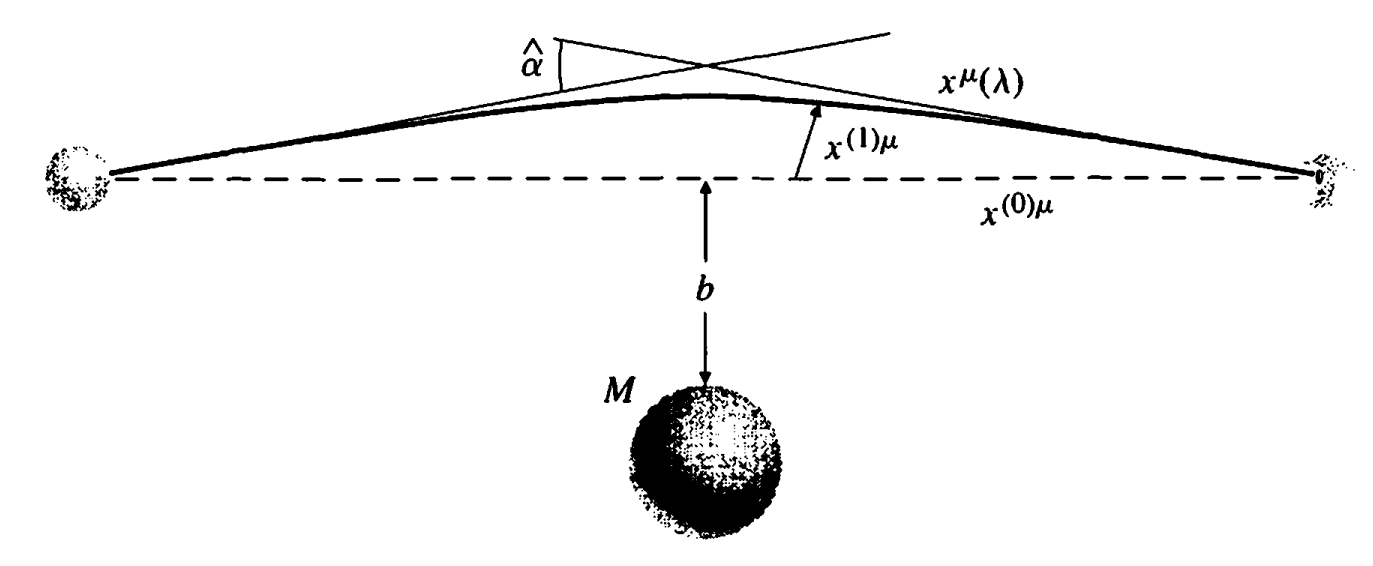
\includegraphics[scale=0.3]{bend}
	\caption{A deflected geodesic $x^\mu(\lambda)$, decomposed into a background geodesic $x^{(0)\mu}$ and a perturbation $x^{(1)u}$. The deflection angle $\hat{\alpha}$ represents (minus) the amount by which the wave vector rotates along the path. A single mass $M$ with impact parameter $b$ is depicted, although the setup is more general.}
\end{figure}

It's important to remember that we consider the metric perturbation as a field defined on a flat background spacetime. With this, we can decompose the geodesic into a background path plus a perturbation:
\begin{align}
x^\mu(\lambda) = x^{(0)\mu}(\lambda) + x^{(1)\mu}(\lambda)
\end{align}
where of course $x^{(0)\mu}(\lambda)$ is just the null (straight) path which solves the flat background geodesic equation. We want to solve for $x^{(1)\mu}(\lambda)$. To do this, we assume that the potential $\phi$ is approximately constant along the background and true geodesics, i.e., $x^{(1)i}\p_i \phi \ll \phi$. This is reasonable assumption, since $x^{(1)\mu}(\lambda)$ is necessarily small. \\

For convenience we denote the derivative of the vector of the background path as $k^\mu$, and the derivative of the deviation vector as $l^\mu$:
\begin{align}
k^\mu \equiv \f{dx^(0)^\mu}{d\lambda}; \quad l^\mu \equiv \f{dx^{(1)\mu}}{d\lambda}.
\end{align}
The null path obeys the condition:
\begin{align}\label{null}
0 &= g_{\mu\nu}\f{dx^\mu}{d\lambda}\f{dx^\nu}{d\lambda}\nn\\
&= \lp \eta_{\mu\nu} + h_{\mu\nu} \rp\f{d\lp x^{(0)\mu} + x^{(1)\mu} \rp}{d\lambda}\f{d\lp x^{(0)\nu} + x^{(1)\nu} \rp}{d\lambda}\nn\\
&= \boxed{\lp \eta_{\mu\nu} + h_{\mu\nu} \rp(k^\mu + l^\mu)(k^\nu + l^\nu)}
\end{align}
At zeroth order we only have 
\begin{align}
\eta_{\mu\nu}k^\mu k^\nu = 0 \implies {\lp k^0\rp}^2 = \vec{k}^2 \equiv k^2.
\end{align}
This defines the constant $k$. At first order, we have
\begin{align}\label{orth}
2\eta_{\mu\nu}k^\mu l^\nu + h_{\mu\nu}k^\mu k^\nu = 0 \implies \boxed{-kl^0 + \vec{l}\cdot \vec{k} = 2k^2 \phi(r)}
\end{align}
since $\lp k^0\rp^2 = \vec{k}^2 = k^2$. Now, we turn to the perturbed geodesic equation:
\begin{align}
\f{d^2 x^\mu}{d\lambda^2} + \Gamma^\mu_{\rho\sigma}\f{dx^\rho}{d\lambda}\f{dx^\sigma}{d\lambda} = 0.
\end{align}
With $\eta_{\mu\nu} = \text{diag}(-\,+\,+\,+)$, the relevant Christoffel symbols are
\begin{align}
&\Gamma^0_{0i} = \Gamma^i_{00} = \p_i \phi\nn\\
&\Gamma^i_{jk} = \delta_{jk}\p_i \phi - \delta_{ik}\p_j\phi - \delta_{ij}\p_k \phi.
\end{align}
The zeroth-order equation simple tells us that $x^{(0)\mu}$ is a straight trajectory, while at first-order we have
\begin{align}
\boxed{\f{d l^\mu}{d\lambda} = -\Gamma^\mu_{\rho\sigma}k^\rho k^\sigma}
\end{align}
When $\mu= 0$, we have
\begin{align}
\boxed{\f{d l^0}{d\lambda} = -2k(\vec{k}\cdot \grad{\phi})}
\end{align}
while the spatial components read
\begin{align}\label{rotate}
\boxed{\f{d\vec{l}}{d\lambda}} &= -2k^2\lp \grad - \vec{\nabla}_\parallel \rp  \phi \nn\\
&\equiv -2k^2\vec{\nabla}_\perp \phi = \boxed{-2k^2\lp \grad{\phi} - k^{-2}(\vec{k}\cdot \grad{\phi})\vec{k} \rp}
\end{align}
where $\vec{\nabla}_\perp$ denotes the gradient of $\phi$ along the deviation and $\vec{\nabla}_\parallel$ denotes the gradient of $\phi$ along the path. \\


Next, we notice that
\begin{align}
l^0 &= \int \f{dl^0}{d\lambda}\,d\lambda\nn\\
&= -2k\int (\vec{k}\cdot \grad{\phi})\,d\lambda\nn\\
&= -2k\int \lp \f{d \vec{x}^{(0)}}{d\lambda}\cdot \grad{\phi}\rp\,d\lambda\nn\\
&= -2k\int \grad{\phi}\cdot d\vec{x}^{(0)}\nn\\
&= -2k\int \p_x \phi \,(\hat{x}\cdot \hat{x})\, d{x}^{(0)}\nn\\
&= -2k \phi.
\end{align}
We can fix the constant of integration by demanding that $l^0 \iff \phi= 0$. It follows from \eqref{orth} that
\begin{align}
\vec{l}\cdot \vec{k} &= 2k^2\phi+ kl^0\nn\\
&=2k^2\phi - 2k^2\phi \nn\\
&= 0.
\end{align}
Thus $\vec{k}\perp \vec{l}$, to first order. This makes intuitive sense if we think about it a little bit.\\

Now, the deflection angle $\hat{\alpha}$ is the amount by which the original spatial wave vector is deflected as it travels from a source to the observer. It is a two-dimensional vector in the plane perpendicular to $\vec{k}$ (by figure) and hence is (anti)-parallel to $\vec{l}$. And by the figure, we can write
\begin{align}
\hat{\alpha} = -\f{\Delta \vec{l}}{k},
\end{align}
where the minus sign accounts for the fact that the deflection angle is measured by an observer looking backward along the photon path. The rotation of the wave vector $\Delta \vec{l}$ can be calculated using \eqref{rotate}:
\begin{align}
\Delta \vec{l} &= \int \f{d\vec{l}}{d\lambda}\,d\lambda \nn\\
&= -2k^2 \int -2k^2\vec{\nabla}_\perp \phi\,d\lambda.
\end{align}  
And with $s = k\lambda$ denoting the physical spatial distance traversed we have
\begin{align}
\boxed{\hat{\alpha} = 2\int \vec{\nabla}_\perp \phi\,ds}
\end{align}
We also have
\begin{align}
\phi(r) = \f{-GM}{r} \implies \phi(x) = \f{-GM}{\sqrt{x^2 + b^2}},
\end{align}
and
\begin{align}
\vec{\nabla}_\perp \phi = \f{d}{db}\phi(x)\hat{b} = \f{GM}{(b^2 + x^2)^{3/2}}\vec{b}.
\end{align}
Putting everything together, followed by a change of variables, we get
\begin{align}
\boxed{\hat{\alpha} = 2GMb\int_{-\infty}^\infty \f{dx}{(b^2 + x^2)^{3/2}} = \f{4GM}{b} = \f{2(1+1)GM}{b}}
\end{align}
and so $\gamma=1$ as desired. The integral from $-\infty$ to $\infty$ assumes that both source and observer are very far from the deflecting mass. \\

What if the form of $h_{\mu\nu}$ is 
\begin{align}
{h_{\mu\nu}= \begin{bmatrix}
	-2\phi(r) & &&\\
	&-2\gamma\phi(r)&&\\
	&&-2\gamma\phi(r)&\\
	&&&-2\gamma\phi(r)
	\end{bmatrix}}?
\end{align}
It is not difficult in this case to recalculate the Christoffel symbols, again using $\eta = \text{diag}(-\,+\,+\,+)$ for consistency:
\begin{align}
&\Gamma^\mu_{00} = \p_i \phi\nn\\
&\Gamma^i_{jk} =  \gamma\lp \delta_{jk}\p_i \phi - \delta_{ik}\p_j \phi - \delta_{ij}\p_k \phi\rp.
\end{align}
Repeating the procedure in the previous paragraphs we find from the null path condition \eqref{null} at zeroth order
\begin{align}
\eta_{\mu\nu}k^\mu k^\nu = 0\implies k^2 = \vec{k}^2 = \lp k^0 \rp^2
\end{align}
and at first order, because $\lp k^0 \rp^2 = \vec{k}^2 = k^2$,
\begin{align}
2\eta_{\mu\nu}k^\mu l^\nu + h_{\mu\nu}k^\mu k^\nu = 0 \implies -kl^0 + \vec{l}\cdot \vec{k} = 2(1+\gamma)k^2\phi(r).
\end{align}    
This factor of $(1+\gamma)$ will reappear when we find the spatial component $d\vec{l}/d\lambda$ since it is embedded in the new Christoffel symbol $\Gamma^i_{\mu\nu}$ (I know this must be true, but I won't verify...)
\begin{align}
\boxed{\f{d\vec{l}}{d\lambda} = -2(1+\gamma)k^2 \vec{\nabla}_\perp \phi}
\end{align}
From here and the rest of the procedure, this factor $(1+\gamma)$ is carried throughout (even to the part where we show $\vec{l}\perp \vec{k}$) and eventually end up in the final integral:
\begin{align}
\boxed{\hat{\alpha} = 2(1+\gamma)GMb\int_{-\infty}^\infty \f{dx}{(b^2 + x^2)^{3/2}} = \f{2(1+\gamma)GM}{b}}
\end{align}
So we're done with the massless case. \qedhere \\














\noindent \underline{\textit{Application of \eqref{light}, massive gravity:}}

In the massive case, the metric $h_{\mu\nu}$ has the form
\begin{empheq}[box=\widefbox]{align*}
&h_{00}(r) = \f{2M}{3M_P}\f{1}{4\pi}\f{e^{-mr}}{r}\nn\\
&h_{0i}(r) = 0\nn\\
&h_{ij}(r) = \f{M}{3M_P}\f{1}{4\pi}\f{e^{-mr}}{r}\lb \f{1+mr+m^2r^2}{m^2r^2} \delta_{ij} - \f{1}{m^2 r^4}(3+3mr + m^2r^2)x_ix_j \rb
\end{empheq}
which is not quite the right form to read off the Newtonian potential and light bending. To simplify things, we notice that while the massive gravity action is not gauge invariant, we assumed tat the coupling to the test particle is that of GR, i.e., this coupling is  gauge invariant. We can argue that we are free to make a gauge transformation on the solution $h_{\mu\nu}$, and there will be no effect on the test particle. To simplify the metric above, i.e. hopefully making it more ``uniformly diagonal'' we can go back to the general expression for $h_{ij}$
\begin{align}
h_{ij}(x) = \f{M}{3M_P}\int \f{d^3\mathbf{p}}{(2\pi)^3}e^{i\mathbf{p}\cdot \mathbf{x}}\f{1}{\mathbf{p}^2 + m^2} \lp \delta_{ij} + \f{p_i p_j}{m^2} \rp
\end{align}
and notice that the term $p_ip_j/m^2$ is pure gauge. This means under some gauge transformation, we can ignore this term (why?). With this, our metric is equivalent to the metric:
\begin{align}
&h_{00}(r) = \f{2M}{3M_P}\f{1}{4\pi}\f{e^{-mr}}{r}\nn\\
&h_{0i}(r) = 0\nn\\
&h_{ij}(r) = \f{M}{3M_P}\f{1}{4\pi}\f{e^{-mr}}{r}
\end{align}
In the small mass limit, this metric becomes
\begin{empheq}[box=\widefbox]{align*}
&h_{00}(r) = \f{2M}{3M_P}\f{1}{4\pi r}\nn\\
&h_{0i}(r) = 0\nn\\
&h_{ij}(r) = \f{M}{3M_P}\f{1}{4\pi r}\delta_{ij}
\end{empheq}
which means when we read off the fields $\phi$ and $\psi$ we find 
\begin{align}
h_{00}(r) = \f{2M}{3M_P}\f{1}{4\pi r} \implies \boxed{\phi(r) = -\f{4}{3}\f{GM}{r}}\nn\\
h_{ij}(r) = \f{M}{3M_P}\f{1}{4\pi r}\delta_{ij} \implies \boxed{ \psi(r) = -\f{2}{3}\f{GM}{r}}
\end{align}
for massive gravitons.\\

The Newtonian potential $\phi$ is larger then for the massless case. The PPN parameter is
\begin{align}
\boxed{\gamma = \f{\psi(r)}{\phi(r)} = \f{1}{2}}
\end{align} 
and thus the magnitude of the light bending angle for light incident at impact parameter $b$ is reduced by $25\%$:
\begin{align}
\boxed{\hat{\alpha} = \f{2(1+ 1/2)GM}{b} = \f{3GM}{b} \neq \f{4GM}{b}}
\end{align}
when we scale $\phi$ so that it matches with the Newtonian potential, even in the massless limit (note that this formula is obtained from the massless theory, so we can only use it here in the massless limit). \\

What this all means is that linearized massive gravity, even in the massless limit, gives predictions which are order 1 different from linearized GR. This is the vDVZ discontinuity. It is present in other physical predictions as well, such as emission of gravitational radiation. Sean Carroll's Chapter 7,\textit{Spacetime \& Geometry} goes over how to derive gravitation radiation (gravitational wave), but we won't worry about that.


















\newpage

\subsection{The St\"{u}ckelberg Trick}

There are a number of ways the St\"{u}ckelberg trick has appeared in literature. Some refer to it as an approach or trick. Some don't even refer to it at all. In this section, we look at some approaches to introducing and using the St\"{u}kelberg trick in the context of massive gravity.\\

We have seen that there is a discontinuity in the physical prediction of linear massless gravity and the massless limit of linear massive gravity, known as the vDVZ discontinuity. We will see explicitly that the correct massless limit of massive gravity is not massless gravity, but rather massless gravity plus extra degrees of freedom. The extra degrees of freedom are a massless vector and a massless scalar, which couples to the trace of the energy momentum tensor. This extra scalar coupling is responsible for the vVDZ discontinuity. \\

Recall the Lagrangian:
\begin{empheq}[box=\widefbox]{align*}
S_{FP} = \int d^Dx\, &-\f{1}{2}\p_\lambda h_{\mu\nu} \p^\lambda h^{\mu\nu} + \p_\mu h_{\nu\lambda}\p^\nu h^{\mu\lambda}\nn\\& - \p_\mu h^{\mu\nu}\p_\nu h + \f{1}{2}\p_\lambda h \p^\lambda h -\f{1}{2}m^2\lp h_{\mu\nu}h^{\mu\nu} - h^2 \rp + \kappa h_{\mu\nu}T^{\mu\nu}
\end{empheq}
Taking the $m\to 0$ straight away here does not yield a smooth limit, since degrees of freedom are lost. To find the correct limit, the \textit{trick} is to introduce new fields and gauge symmetries into the massive theory in a way that does not alter the theory. This is called the St\"{u}ckelberg trick. Once this is done, a limit can be found in which no degrees of freedom are gained or lost. 

\subsubsection{Motivation}

The goal of the St\"{u}kelberg trick is to make a massive theory gauge invariant. As we have seen, the massive term in the Fierz-Pauli action breaks diffeomorphism. The St\"{u}kelberg mechanism is the introduction of new field(s) to a reveal a symmetry of a gauge-fixed theory. \\

In general, dynamical tensors $K_{\mu\nu}$ transform under diffeomorphisms as
\begin{align}
K_{\mu\nu} \to &\,\,K_{\mu\nu} + \lag_3 K_{\mu\nu} \nn\\
&= K_{\mu\nu} + (\p_\mu \epsilon^\alpha)K_{\alpha\nu} + (\p_\nu \epsilon^\alpha)K_{\mu\alpha} + \epsilon^\alpha \p_\alpha K_{\mu\nu}.
\end{align}
However, nondynamical background $\bar{K}_{\mu\nu}$ obeys
\begin{align}
\bar{K}_{\mu\nu} \to \bar{K}_{\mu\nu}.
\end{align}

In the context of massive gravity, in the nonlinear regime, we want to couple a mass to $g_{\mu\nu}$. But we also want to avoid $g^{\mu\nu}g_{\mu\nu} = 4$, so we must introduce a nondynamical background $\bar{K}_{\mu\nu}$ such that the mass terms become $\sim (\bar{K}^{\mu\nu}g_{\mu\nu})^2$, which break diffeomorphism.  \\

St\"{u}kelberg's trick puts back diffeomorphism invariance while introducing 4 scalars $\phi^a, a = 0,1,2,3$ such that we gain/lose no degree of freedom. To do this, we can replace
\begin{align}
\bar{K}_{\mu\nu}(x) \to \p_\mu \phi^a \p_\nu \phi^b \bar{K}_{ab}(\phi(x)).
\end{align}
Here $\phi^a$ is a dynamical scalar with which we can restore diffeomorphism invariance in the theory. (We will see later why we would like to make this replacement/definition.)\\

How is diffeomorphism restored? Well first we can fix
\begin{align}
\phi^a = \delta^a_\alpha x^\alpha,
\end{align} 
where $x^\alpha$ is literally just the coordinate, such that
\begin{align}
\p_\mu \phi^a = \delta^a_\alpha \delta^\alpha_\mu = \delta^a_\mu.
\end{align}
So we have
\begin{align}
\p_\mu \phi^a\p_\nu \phi^b \bar{K}_{ab}(\phi) &= \delta^a_\mu \delta^b_\nu \bar{K}_{ab} \nn\\
&= \bar{K}_{\mu\nu}(x).
\end{align}
So we see this choice of gauge fixing gives the desired transformation. Next, suppose we look at excitations of the form
\begin{align}
\phi^a = \delta^a_\alpha(x^\alpha +\pi^\alpha)
\end{align}
where $\pi^\alpha$ are fields that are like th Nambu-Goldstone modes, then
\begin{align}
\p_\mu \phi^a &= \delta^a_\mu + \p_\mu \pi^\alpha \delta^a_\alpha\nn\\
&= \delta^a_\mu + \p_\mu \pi^a.
\end{align}
With this,
\begin{align}
\p_\mu \phi^a \p_\nu \phi^b \bar{K}_{ab} &= (\delta^a_\mu + \p_\mu \pi^a)(\delta^b_\nu + \p_\nu \pi^b)\bar{K}_{ab}(x+\pi)\nn\\
&\approx  (\delta^a_\mu + \p_\mu \pi^a)(\delta^b_\nu + \p_\nu \pi^b)(\bar{K}_{ab} + \pi^\alpha \p_\alpha K_{ab}(x) + \dots)\nn\\
&\approx \bar{K}_{\mu\nu} + (\p_\mu \pi^a)\bar{K}_{a\nu} + (\p_\nu \pi^b)\bar{K}_{\mu b} + \pi^\alpha \p_\alpha \bar{K}_{\mu\nu} + \dots
\end{align}
up to first order in $\pi$. The first approximation is just an affine approximation of $\bar{K}_{ab}$. This puts the Nambu-Goldstone modes back into the theory with explicit breaking, when $\pi^\mu$ are like Nambu-Goldstone modes. This turns out to have local symmetry. We can always gauge fix so that $\p^\mu \to 0$ and get back the original theory. \\

A lot of this seems very arbitrary and sort of ``out-of-nowhere.'' But rest assured, as we will see what we are actually doing by introducing $\phi^a$ and how this trick works in the next section.






\subsubsection{The St\"{u}ckelberg's Trick - a Vector Example (Hinterbichler)}

To see how the trick works, we consider a simple case of the theory of a massive photon $A_\mu$ coupled to a (not necessarily conserved) source $J_\mu$:
\begin{align}
S = \int d^Dx\, -\f{1}{4}F_{\mu\nu}F^{\mu\nu} - \f{1}{2}m^2 A_\mu A^\mu + A_\mu J^\mu.
\end{align}
where of course
\begin{align}
F_{\mu\nu} = \p_\mu A_\nu - \p_\nu A_\mu
\end{align}
is the anti-symmetric EM stress-tensor. The mass term break the would-be gauge invariance:
\begin{align}
A_\mu \to A_\mu + \p_\mu \Lambda \iff \delta A_\mu = \p_\mu \Lambda,
\end{align}
and for $D=4$ this theory describes the 3 degrees of freedom of a massive spin 1 particle. The propagator for this theory is given by
\begin{align}
\f{-i}{p^2 + m^2}\lp \eta_{\mu\nu} +\f{p_\mu p_\nu}{m^2} \rp
\end{align}
which is not quite as nice as the usual massless photon propagator (Maxwell theory) due to $m\neq 0$, and is similar to $\sim 1/m^2$ for large momenta. This property invalidates the usual power-counting arguments.\\

The limit $m\to 0$ of the Lagrangian above is not a smooth limit because we lose a degree of freedom: for $m=0$ we have Maxwell's EM theory which propagates only with 2 degrees of freedom. Also, the limit fails to exist unless $J^\mu$ is conserved. \\

Here's how the St\"{u}ckelberg trick works. The trick consists of introducing a new scalar field $\phi$ such  tat the new action has gauge symmetry but is still dynamically equivalent to the original action. It will give a different $m\to 0$ smooth limit such that no degrees of freedom are gained or lost. \\

Let us begin by introducing  a field $\phi$ by making the replacement:
\begin{align}
A_\mu \to A_\mu + \p_\mu \phi
\end{align}
following the pattern of the gauge symmetry we want to introduce. This is \textit{not} a change of field variables, a decomposition of $A_\mu$, nor a gauge transformation (remember, this new theory breaks gauge invariance). Rather, we are creating a new Lagrangian from th old one, by the addition of a new field $\phi$. $F_{\mu\nu}$ is invariant under this replacement because the replacement is similar to a gauge transformation under which $F_{\mu\nu}$ is invariant. The only thing that changes is the mass term and the coupling to the source. Following some simple algebra, the action becomes
\begin{align}
S = \int d^Dx\, -\f{1}{4}F_{\mu\nu}F^{\mu\nu} -\f{1}{2}m^2\lp A_\mu + \p_\mu \phi \rp^2 + A_\mu J^\mu - \phi \p_\mu J^\mu
\end{align} 
where we have integrated by parts in the coupling to the source. The new action now has the gauge symmetry:
\begin{align}
\delta A_\mu = \p_\mu \Lambda; \quad \delta \phi = -\Lambda.
\end{align}
By fixing the gauge $\phi = 0$, called the unitary gauge, we recover the original Lagrangian:
\begin{align}
S = \int d^Dx\, -\f{1}{4}F_{\mu\nu}F^{\mu\nu} - \f{1}{2}m^2 A_\mu A^\mu + A_\mu J^\mu.
\end{align}
This tells us that the action with $\phi = 0$ and $\phi \neq 0$ are equivalent theories. They both describe the 3 d.o.f of a massive spin 1 in 4-dimensional spacetime. The new Lagrangian just has more fields and symmetries. Pro tip: when introducing new fields, make sure to introduce new symmetries so as to conserve degrees of freedom. \\

The St\"{u}ckelberg trick uses redundancy (introduces new fields as well as new symmetries) to fix theories. The St\"{u}ckelberg trick adds and removes extra gauge symmetry in a way that does not mess with the manifest Lorentz invariance and locality. \\

Now, consider the new theory again:
\begin{align}
S = \int d^Dx\, -\f{1}{4}F_{\mu\nu}F^{\mu\nu} -\f{1}{2}m^2\lp A_\mu + \p_\mu \phi \rp^2 + A_\mu J^\mu - \phi \p_\mu J^\mu.
\end{align} 
By normalizing $\phi \to m^{-1}\phi$, we get
\begin{align}
S = \int d^Dx\, \f{-1}{4}F_{\mu\nu}F^{\mu\nu} -\f{m^2}{2} A_\mu A^\mu - mA_\mu \p^\mu \phi - \f{1}{2}\p_\mu \phi \p^\mu \phi + A_\mu J^\mu-\f{1}{m}\phi \p_\mu J^\mu.
\end{align}
The gauge symmetries after this normalization is:
\begin{align}
\delta A_\mu = \p_\mu \Lambda; \quad \delta \phi = -m\Lambda.
\end{align}
Now, consider the $m\to 0$ limit. If $\p_\mu  J^\mu \neq 0$, i.e., the current is not conserved, then when $m \ll 1$, the scalar field $\phi$ couples strongly with the divergence of source, and the limit does not exist. This requires us to assume the current to be conserved: $\p_\mu J^\mu = 0$. This implies the new theory in the $m\to 0$ limit is 
\begin{align}
\lag = -\f{1}{4}F_{\mu\nu}F^{\mu\nu} - \f{1}{2}\p_\mu \phi \p^\mu \phi + A_\mu J^\mu,
\end{align}
endowed with the gauge symmetries ($m=0$):
\begin{align}
\delta A_\mu = \p_\mu \Lambda; \quad \delta \phi = 0.
\end{align}
The degrees of freedom turn out to be conserved in the limit. For $D=4$ two of the 3 degrees of freedom go into the massless vector,and one goes into the scalar. \\

We can fix a Lorentz-like gauge:
\begin{align}
\p_\mu A^\mu + m\phi = 0
\end{align}
which along with the gauge symmetries: $\delta A_\mu = \p_\mu \Lambda; \quad \delta \phi = -m\Lambda$ satisfies $(\square - m^2)\Lambda = 0$. From Fadeev-Popov, we add a this gauge fixing term (which is zero) to the action to get
\begin{align}
S+ S_{GF} &= S + \int d^Dx\, -\f{1}{2}\lp \p_\mu A^\mu + m\phi \rp^2\nn\\
&= \dots\nn\\
&= \boxed{\int d^Dx\, \f{1}{2}A_\mu (\square - m^2)A^\mu + \f{1}{2}\phi(\square - m^2)\phi + A_\mu J^\mu - \f{1}{m}\phi \p_\mu J^\mu}
\end{align} 
From there, we can pick out the propagators for $A_\mu$ and $\phi$ in momentum space respectively:
\begin{align}
\boxed{\D_{A_\mu}(p) = \f{-i\eta_{\mu\nu}}{p^2 + m^2}; \quad \D_{\phi}(p) = \f{-i}{p^2 + m^2}}
\end{align}
These go as $\sim 1/p^2$ at high momenta. So, we are able to restore good high energy behavior of the theory propagators. 
























\subsubsection{Graviton St\"{u}ckelberg's Trick \& The origin of the vDVZ discontinuity (Hinterbichler)}

Now, let us consider the massive gravity action, which is made up of the massless piece, plus the mass term, plus the source coupling term:
\begin{align}
\boxed{S = \int d^Dx\, \lag_{m=0} - \f{1}{2}m^2\lp h_{\mu\nu}h^{\mu\nu} - h^2 \rp + \kappa h_{\mu\nu}T^{\mu\nu}}
\end{align}
We want to preserve (or restore(?)) the diffeomorphism:
\begin{align}
\delta h_{\mu\nu} = \p_\mu \epsilon_\nu + \p_\nu \epsilon_\mu = \p_{(\mu}\epsilon_{\nu)}
\end{align}
present in the $m=0$ case, so we introduce a St\"{u}ckelberg field $A_\mu$ patterned after the gauge transformation/symmetry:
\begin{align}\label{stuck}
\boxed{h_{\mu\nu} \to h_{\mu\nu} + \p_\mu A_\nu + \p_\nu A_\mu}
\end{align}
What does the action look like following this transformation? Some quick manipulations give
\begin{empheq}[box=\widefbox]{align*}
S = \int d^Dx\, &\lag_{m=0} - \f{1}{2}m^2\lp h_{\mu\nu}h^{\mu\nu} - h^2 \rp - \f{1}{2}m^2 F_{\mu\nu}F^{\mu\nu}\nn\\
&-2m^2\lp h_{\mu\nu} \p^\mu A^\nu - h\p_\mu A^\mu \rp + \kappa h_{\mu\nu}T^{\mu\nu} - 2\kappa A_\mu \p_\nu T^{\mu\nu}
\end{empheq}
where we notice that $\lag_{m=0}$ term is invariant under this transformation (since it is the originally gauge-invariant Lagrangian). Other terms are not invariant under the transformation above in $h_{\mu\nu}$. We also note that we are setting $F_{\mu\nu} = \p_\mu A_\nu - \p_\mu A_\nu$, and that we integrated the last term by parts to bring the $\p$ inside to act on $T^{\mu\nu}$ instead of on $A_\mu$. \\

Just as before, we observe two gauge symmetries:
\begin{align}
\delta h_{\mu\nu} = \p_\mu \epsilon_\nu + \p_\nu \epsilon_\mu; \quad \delta A_\mu = -\epsilon_\mu.
\end{align}
Fixing the gauge $A_\mu = 0$ gives back the massive gravity action (without extra fields, etc.). At this point, if we try to repeat what we did before: rescaling $A_\mu \to m^{-1}A_\mu$, we will fail because when the $m\to 0$ limit is taken, we end up with a massless graviton and a massless photon for a total of 4 degrees of freedom - one less than the desired value of 5. \\

Instead, we go further and introduce a St\"{u}ckelberg field $\phi$ and consider the transformation:
\begin{align}
A_\mu \to A_\mu + \p_\mu \phi,
\end{align}
under which the action above becomes:
\begin{empheq}[box=\widefbox]{align*}
S = \int d^Dx\, &\lag_{m=0} - \f{1}{2}m^2\lp h_{\mu\nu}h^{\mu\nu} - h^2 \rp - \f{1}{2}m^2 F_{\mu\nu}F^{\mu\nu}\nn\\
&-2m^2\lp h_{\mu\nu} \p^\mu A^\nu - h\p_\mu A^\mu \rp -2m^2\lp h_{\mu\nu}\p^\mu \p^\nu \phi - h\square \phi \rp\nn\\
&+\kappa h_{\mu\nu}T^{\mu\nu} - 2\kappa A_\mu \p_\nu T^{\mu\nu} + 2\kappa \phi \p \p T
\end{empheq}
where 
\begin{align}
\p \p T \equiv \p_\mu \p_\nu T^{\mu\nu}.
\end{align}
With the introduction of the scalar field $\phi$, we must also include two more gauge symmetries to the theory, giving 4 total gauge symmetries, which follow from the redefinition \eqref{stuck} 
\begin{align}
\begin{cases}
\delta h_{\mu\nu} = \p_\mu \epsilon_\nu + \p_\nu\epsilon_\mu\nn\\
\delta A_\mu = -\epsilon_\mu \nn\\
\delta A_\mu= \p_\mu \Lambda\nn\\
\delta \phi = -\Lambda.
\end{cases}
\end{align}
Once again, by fixing the gauge $\phi = 0$ we get back the previous Lagrangian. \\

Now, we scale:
\begin{align}
A_\mu &\to \f{1}{m}A_\mu\nn\\
\phi &\to \f{1}{m^2}\phi.
\end{align}
The action changes accordingly as
\begin{empheq}[box=\widefbox]{align*}
S = \int d^Dx\, &\lag_{m=0} - \f{1}{2}m^2\lp h_{\mu\nu}h^{\mu\nu} - h^2 \rp - \f{1}{2} F_{\mu\nu}F^{\mu\nu}\nn\\
&-2m\lp h_{\mu\nu} \p^\mu A^\nu - h\p_\mu A^\mu \rp -2\lp h_{\mu\nu}\p^\mu \p^\nu \phi - h\square \phi \rp\nn\\
&+\kappa h_{\mu\nu}T^{\mu\nu} - \f{2}{m}\kappa A_\mu \p_\nu T^{\mu\nu} + \f{2}{m^2}\kappa \phi \p \p T,
\end{empheq}
and the gauge transformations become:
\begin{align}
\begin{cases}
\delta h_{\mu\nu} = \p_\mu \epsilon_\nu + \p_\nu\epsilon_\mu\nn\\
\delta A_\mu = -m\epsilon_\mu \nn\\
\delta A_\mu = \p_\mu \Lambda\nn\\
\delta \phi = -m\Lambda.
\end{cases}
\end{align}
which is quite obvious since we just rescaled things. Now, in the $m \to  0$ limit, we can see that $A_\mu$ and $\phi$ are strongly coupled to the divergence of the source $\p T$ and $\p \p T$. So suppose that the source $T$ is conserved, in which case $\p_\mu T^{\mu\nu} = 0$, then in this limit the theory takes the form
\begin{align}
\boxed{S = \int d^Dx\, \lag_{m=0}  - \f{1}{2} F_{\mu\nu}F^{\mu\nu}  -2\lp h_{\mu\nu}\p^\mu \p^\nu \phi - h\square \phi \rp +\kappa h_{\mu\nu}T^{\mu\nu} }
\end{align} 
This theory has 5 degrees of freedom: a scalar-tensor vector theory where the vector is completely decoupled ($A_\mu$ is completely contained and isolated in the $F_{\mu\nu}$ term) but the scalar is kinetically mixed with the tensor (the mixed term is the one with $h_{\mu\nu}$ and $\phi$). \\


To unmix the coupling between the tensor field $h_{\mu\nu}$ and the scalar field $\phi$ we introduce a field definition:
\begin{align}\label{new-hh}
\boxed{h_{\mu\nu} = h'_{\mu\nu} + \pi \eta_{\mu\nu}}
\end{align}
where $\pi$ is some scalar field. Under this field substitution, the massless Lagrangian becomes:
\begin{align}
\lag_{m=0}(h) &= -\f{1}{2}\p_\lambda h_{\mu\nu} \p^\lambda h^{\mu\nu} + \p_\mu h_{\nu\lambda}\p^\nu h^{\mu\lambda} - \p_\mu h^{\mu\nu}\p_\nu h + \f{1}{2}\p_\lambda h \p^\lambda h \nn\\
&= \dots\nn\\
&= \lag_{m=0}(h') + (D-2)\lb \p_\mu \pi \p^\mu h' - \p_\mu \pi \p_\nu h'^{\mu\nu} + \f{1}{2}(D-1)\p_\mu \pi \p^\mu \pi \rb.
\end{align}
Now, by setting
\begin{align}
\pi = \f{2}{D-2}\phi,
\end{align}
we can unmix the $h-\phi$ coupling in the original Lagrangian. After some simplifications, we obtain the new action following the field substitution:
\begin{align}
\boxed{S = \int d^Dx\,\lag_{m=0}(h') - \f{1}{2}F_{\mu\nu}F^{\mu\nu} - 2\f{D-2}{D-1}\p_\mu \phi \p^\mu \phi + \kappa h'_{\mu\nu}T^{\mu\nu} + \f{2}{D-2}\kappa \phi T}
\end{align}
The gauge symmetries in this theory are
\begin{align}
\begin{cases}
\delta h'_{\mu\nu} = \p_\mu \epsilon_\nu + \p_\nu \epsilon_\mu \nn\\
\delta A_\mu = 0\nn\\
\delta A_\mu = \p_\mu \Lambda\nn\\
\delta \phi = 0.
\end{cases}
\end{align}
which follow from the field redefinition \eqref{new-hh}. With $D=4$, there are 5 degrees of freedom: two in a canonical massless graviton, two in a canonical massless vector, and one in a canonical massless scalar. \\

However, notice that there is still a coupling between the scalar $\phi$ and the trace of the source $T$ (even) in the $m=0$ limit. This is the origin of the vDVZ discontinuity. When we consider the trajectory of light, we set $T=0$, so this does not affect the bending of light. However, this extra scalar degree of freedom affects the Newtonian potential. We actually have seen this earlier. To reconcile the disagreement in the predicted bending angle of light $\hat{\alpha} \sim 4GM/b \neq 3GM/b$, we will have to rescale the gravitational constant $G$ which affects the Newtonian potential.\\

In the $m\neq 0$ regime with not necessarily conserved source, under the field redefinition:
\begin{align}\label{new-h}
\boxed{h_{\mu\nu} = h'_{\mu\nu} + \f{2}{D-2}\phi \eta_{\mu\nu}}
\end{align}
which follows from setting $\pi = 2\phi/(D-2)$, the full action is given by (ready?)
\begin{empheq}[box=\widefbox]{align*}
S = &\int d^Dx\, \lag_{m=0}(h') - \f{1}{2}m^2 \lp h'_{\mu\nu}h'^{\mu\nu} - h'^2 \rp - \f{1}{2}F_{\mu\nu}F^{\mu\nu}\nn\\
&+ 2\f{D-1}{D-2}\phi \lp \square + \f{D}{D-2}m^2 \rp\phi - 2m\lp h'_{\mu\nu}\p^\mu A^\nu - h' \p_\mu A^\mu \rp + \kappa h'_{\mu\nu}T^{\mu\nu} \nn\\
&+ 2\f{D-1}{D-2}\lp m^2 h'\phi+ 2m \phi \p_\mu A^\mu \rp  +  \f{2}{D-2}\kappa \phi T - \f{2}{m}\kappa A_\mu \p_\nu T^{\mu\nu} + \f{2}{m^2}\kappa \phi \p \p T.
\end{empheq}
(whose verification is left as an ``index-swimming'' exercise to the reader). This theory has the following gauge symmetries:
\begin{align}
\begin{cases}
\delta h'_{\mu\nu} = \p_\mu \epsilon_\nu + \p_\nu \epsilon_\mu + \f{2}{D-2}m \Lambda \eta_{\mu\nu}\nn\\
\delta A_\mu = -m\epsilon_\mu\nn\\
\delta A_\mu = \p_\mu \Lambda\nn\\
\delta \phi = -m\Lambda.
\end{cases}
\end{align}
It looks like the gauge symmetries has drastically changed, but if we look carefully there is not much going on here. From the field redefinition we can see how the first gauge symmetry is obtained:
\begin{align}
h_{\mu\nu} = h'_{\mu\nu} + \f{2}{D-2}\phi \eta_{\mu\nu} \implies \delta h'_{\mu\nu} &= \delta h_{\mu\nu} - \f{2}{D-2}(\delta \phi) \eta_{\mu\nu}\nn\\
&= \p_\mu \epsilon_\nu + \p_\nu \epsilon_\mu - \f{2}{D-2}(\delta \phi) \eta_{\mu\nu}\nn\\
&= \p_\mu \epsilon_\nu + \p_\nu \epsilon_\mu + \f{2}{D-2}m\Lambda \eta_{\mu\nu}
\end{align}
which follows from the fact that
\begin{align}
\delta \phi = -m\Lambda
\end{align}
after defining $A_\mu \to A_\mu + \p_\mu \phi$, and rescaling $A_\mu \to (1/m)A_\mu$ and $\phi \to (1/m^2)\phi$. In any case, these are minor details we don't have to worry about too much. \\

Now, remember that in order to find the propagators for these fields (scalar $\phi$, vector $A_\mu$, and tensor $h_{\mu\nu}$), we must be able to invert the differential operators that correspond to each field in the Lagrangian. Since there are gauge symmetries, these differential operators don't have trivial kernel (i.e. not invertible). This requires some gauge-fixing to allow for operator inversion. There are 2 gauge conditions we would like to fix: one in $\Lambda$ and one in $\epsilon_\mu$. These are the residual ``degrees of freedom'' that we need to eliminate for things to be invertible. \\

We can try to fix the $\epsilon_\mu$ symmetry first. From the gauge symmetries, we observe that if we say
\begin{align}
\p^\nu h'_{\mu\nu} - \f{1}{2}\p_\mu h' + mA_\mu = 0
\end{align}
then we can fix the $\epsilon_\mu$ symmetry up to a residual transformation satisfying
\begin{align}
(\square - m^2)\epsilon_\mu = 0,
\end{align}
which is good, except it is invariant under $\Lambda$ transformations. This requires fixing the $\Lambda$ symmetry. We observe that by fixing 
\begin{align}
\p_\mu A^\mu + m\lp \f{1}{2}h' + 2\f{D-1}{D-2}\phi \rp = 0
\end{align} 
we fix the $\Lambda$ symmetry up to a residual transformation satisfying 
\begin{align}
(\square - m^2)\Lambda = 0.
\end{align}

Thus, we impose the following gauge conditions:
\begin{empheq}[box=\widefbox]{align*}
\p^\nu h'_{\mu\nu} - \f{1}{2}\p_\mu h' + mA_\mu = 0\nn\\
\p_\mu A^\mu + m\lp \f{1}{2}h' + 2\f{D-1}{D-2}\phi \rp = 0
\end{empheq}


Once we have these two gauges, we can add the following gauge-fixing terms (which are just zeros by gauge-fixing)
\begin{align}
\boxed{S_{GF1} = \int d^Dx\, -\lp \p^\nu h'_{\mu\nu} - \f{1}{2}\p_\mu h' + mA_\mu  \rp^2 }
\end{align}
and
\begin{align}
\boxed{S_{GF2} = \int d^Dx\, -\lb \p_\mu A^\mu + m\lp \f{1}{2}h' + 2\f{D-1}{D-2}\phi \rp  \rb^2 }
\end{align}
to the full action (just as we have done before with the original harmonic gauge) to obtain
\begin{empheq}[box=\widefbox]{align*}
S + S_{GF1} + S_{GF2} &= \int d^Dx\, \lb \f{1}{2}h'_{\mu\nu}\lp \square - m^2\rp h'^{\mu\nu} - \f{1}{4}h'\lp \square - m^2 \rp h'\rb\nn\\
&+ \lb A_\mu \lp \square - m^2 \rp A^\mu \rb+ \lb 2\f{D-1}{D-2}\phi   \lp \square - m^2 \rp\phi \rb\nn\\
&\kappa h'_{\mu\nu}T^{\mu\nu} + \f{2}{D-2}\kappa \phi T - \f{2}{m}\kappa A_\mu \p_\nu T^{\mu\nu} + \f{2}{m^2}\kappa \phi \p \p T
\end{empheq}
Recall that the sole purpose of doing this is so that we can write the integrand (the Lagrangian) in terms of the fields and propagators (refer to the part about gauge harmonic for details). In other words, by adding these gauge-fixing terms, we in effect ``diagonalize'' the action. \\

With the action in propagator form, we can read off the propagators of $h'_{\mu\nu}$, $A_\mu$, and $\phi$ respectively:
\begin{align}
\D[h](p) = \f{-i}{p^2 + m^2}\lb \f{1}{2}\lp \eta_{\alpha\sigma}\eta_{\beta\lambda} + \eta_{\alpha\lambda}\eta_{\beta\sigma} \rp - \f{1}{D-2}\eta_{\alpha\beta}\eta_{\sigma\lambda} \rb,
\end{align}
\begin{align}
\D[A](p) = \f{1}{2}\f{-i\eta_{\mu\nu}}{p^2+m^2},
\end{align}
\begin{align}
\D[\phi](p) = \f{D-2}{4(D-1)}\f{-i}{p^2+m^2}
\end{align}
which all behave as $\sim 1/p^2$ at high momenta, so we can apply the usual power-counting methods. These propagators might look a bit unusual, but when we set $D=4$,
\begin{align}
\D[h](p) = \f{-i}{p^2 + m^2}\f{1}{2}\lb \eta_{\alpha\sigma}\eta_{\beta\lambda} + \eta_{\alpha\lambda}\eta_{\beta\sigma}  - \eta_{\alpha\beta}\eta_{\sigma\lambda} \rb,
\end{align}
\begin{align}
\D[A](p) = \f{1}{2}\f{-i\eta_{\mu\nu}}{p^2+m^2},
\end{align}
and
\begin{align}
\D[\phi](p) = \f{1}{6}\f{-i}{p^2+m^2}
\end{align}
we see that these are the propagators we have seen before, and the differential operator-containing terms in the action can be written as
\begin{align}
\int d^Dx\, \f{1}{2} f_{\dots} \mathcal{O}^{\dots} f_{\dots}
\end{align}
for each corresponding field $f$ (scalars, vectors, tensors, etc.) where $\mathcal{O}^{\dots}$ is the inverse of the spatial propagator $\D[f](x)$. I won't worry too much about the details here, because we're not getting any new insights.  












\newpage


\subsection{Nonlinear Massive Gravity}

Up to this point, we have studied only the linear theory of massive gravity, which is determined by the requirement that it propagates only one massive spin 2 degree of freedom. We now turn to the study of the possible interactions and non-linearities for massive gravity. 


\subsubsection{Massive General Relativity}



Recall the original Einstein-Hilbert action for gravity:
\begin{align}
S = \f{1}{16\pi G}\int d^Dx\, \sqrt{-g}R\equiv \int d^Dx\, \sqrt{-g}M_P^2R
\end{align}
where $R$ is the Ricci scalar, and $M_P \equiv 1/4\pi G$ is the Planck mass. By Hinterbichler's convention, however, $M_P^2 \equiv 1/8\pi G$, so we will be following this convention and write
\begin{align}
S = \f{1}{2\kappa^2}\int d^Dx\, \sqrt{-g}R
\end{align}
where $\kappa  \equiv 1/M_P$ in Hinterbichler's convention. \\

What we want in a full theory of massive gravity is some nonlinear theory whose linear expansion around some background is the massive Fierz-Pauli theory. This theory is no longer GR (or Einstein gravity) in general, because we no longer have an obvious gauge invariance constraint.\\

Our first modification to the original GR is adding the Fierz-Pauli term to the full nonlinear GR action. Doing this implies that all nonlinear interactions are due to GR. The addition of the Fierz-Pauli term is given by
\begin{align}
\boxed{S = \f{1}{2\kappa^2}\int d^Dx\, \lb \sqrt{-g}R - \sqrt{-g^{(0)}}\f{1}{4}m^2 g^{(0)\mu\alpha}g^{(0)\nu\beta}\lp h_{\mu\nu}h_{\alpha\beta} - h_{\mu\alpha}h_{\nu\beta} \rp \rb}
\end{align}
where 
\begin{align}
\boxed{h_{\mu\nu} = g_{\mu\nu} - g^{(0)}_{\mu\nu}}
\end{align}
The Lagrangian now explicitly depends on a fixed metric $g^{(0)}_{\mu\nu}$, called the \textit{absolute metric}, on which the massive graviton $h_{\mu\nu}$ propagates. This means contraction, raising, and lowering of indices of $h_{\mu\nu}$ are done via $g^{(0)}_{}\mu\nu$, and not $g_{\mu\nu}$, which is the full metric. This is similar to what we had before, where $\eta_{\mu\nu}$ was responsible general ``index-manipulation.'' The presence of this absolute metric in the mass term breaks the diffeomorphism invariance of the Einstein-Hilbert term. \\

Varying this action with respect to $g_{\mu\nu}$ (the full metric, NOT the perturbation $h_{\mu\nu}$), we find the following equation of motion
\begin{align}
\boxed{0 = \sqrt{-g}\lp R^{\mu\nu} - \f{1}{2}Rg^{\mu\nu} \rp + \sqrt{-g^{(0)}}\f{m^2}{2}\lp g^{(0)\mu\alpha}g^{(0)\nu\beta}h_{\alpha\beta} - g^{(0)\alpha\beta}h_{\alpha\beta}g^{(0)\mu\nu}\rp}
\end{align} 
(\textbf{Fun Exercise: How was this found?}) We see that because we're varying with respect to the full metric $g_{\mu\nu}$, which contracts (and raises and lowers, etc.) the indices of $R_{\mu\nu}$, we just get back the Einstein tensor $G^{\mu\nu} \equiv R^{\mu\nu} - (1/2)Rg^{\mu\nu}$ for the first term in the action. The second term is bit more tricky. I will get back to how we take the variational derivative of the second term with respect to $g_{\mu\nu}$ later when I have time. We actually don't have to worry too much about this result, since we are interested in a much more general Fierz-Pauli potential. In addition to this, we will later see that we can in fact raise/lower indices of $h$ using $g_{\mu\nu}$, except we must also find the correct relationship between the coefficients in the $g^{(0)}_{\mu\nu}$ and the $g_{\mu\nu}$ variational derivatives.\\

In any case, we observe that if the absolute metric $g^{(0)}_{\mu\nu}$ satisfies the Einstein equations, then $g^{(0)}_{\mu\nu} = g^{\mu\nu} \iff h_{\mu\nu} = 0$ is a solution. In this case, we just get back the original GR. When dealing with massive gravity and more complicated nonlinear solutions thereof, we can have two background structures. On one hand, we can have the \textit{absolute metric}, which breaks diffeomorphism. On the other, there is the background metric, which is a solution to the full nonlinear equations, about which we may expand the action. Often the solution metric we are expanding around will be the same as the absolute metric, but if we were expanding around a different solution, say a black hole, there would be two distinct structures: the black hole solution and the absolute metric.  \\

We are interested in more general interactions beyond the action provided above. We will be adding interaction terms with no derivatives, since these are most important at low energies. The most general such potential which reduces to Fierz-Pauli at quadratic order involves adding terms cubic and higher in $h_{\mu\nu}$ in all possible ways. With this, we write in general:
\begin{align}\label{general-massive}
\boxed{S = \f{1}{2\kappa^2}\int d^Dx\, \lb \sqrt{-g}R - \sqrt{-g^{(0)}}\f{1}{4}m^2 U(g^{(0)},h) \rb}
\end{align}
The interaction potential $U$ is the most general one that reduces to Fierz-Pauli at linear order. The power series representation of this potential $U$ is given by
\begin{align}
U(g^{(0)},h) &= \sum^N_{n=2}U_n(g^{(0)},h) \nn\\
&= U_2(g^{(0)},h) + U_3(g^{(0)},h) + U_4(g^{(0)},h) + U_5(g^{(0)},h) + \dots
\end{align}
where just as before
\begin{align}
U_2(g^{(0)},h) &= g^{(0)\mu\alpha}g^{(0)\nu\beta}\lp h_{\mu\nu}h_{\alpha\beta} - h_{\mu\alpha}h_{\nu\beta} \rp   \nn\\
&= \underbrace{g^{(0)\mu\alpha}g^{(0)\nu\beta}h_{\mu\nu}h_{\alpha\beta}}_{\equiv [h^2]} - \underbrace{g^{(0)\mu\alpha}h_{\mu\alpha}g^{(0)\nu\beta}h_{\nu\beta}}_{\equiv [h]^2}\nn\\
&= [h^2] - [h]^2
\end{align}
and further
\begin{align}
U_3(g^{(0)},h) &= C_1[h^3] + C_2[h^2][h] + C_3[h]^3\nn\\
U_4(g^{(0)},h) &= D_1[h^4] + D_2[h^3][h] + D_3[h^2]^2 + D_4[h^2][h]^2 + D_5[h]^4\nn\\
U_5(g^{(0)},h) &= F_1[h^5] + F_2[h^4][h] + F_3[h^3][h]^2 + F_4[h^3][h^2]\nn\\ &\,\,\,\,\,\,+ F_5[h^2]^2[h] + F_6[h^2][h]^3 + F_7[h]^5\nn\\
&\vdots
\end{align}
The square bracket indicates a trace, with indices raised with $g^{(0)\mu\nu}$:
\begin{align}
&[h] = g^{(0)\mu\nu}h_{\mu\nu},\nn\\
&[h^2] = g^{(0)\mu\nu}h_{\mu\nu}g^{(0)\alpha\beta}h_{\alpha\beta} \nn\\
&\vdots
\end{align}
The coefficients $C_k$ are generic. Note that the dimension of $\vec{C_k}$ in $U_n(g^{(0)},h)$ whenever $n>D$ is actually redundant by 1, not $n$, because of Cayley-Hamiltonian theorem, which guarantees that existence of combination of the contractions (the combination that is the characteristic polynomial $\lag_h^{TD}(h)$) that annihilates $U_n(g^{(0)}_h)$. This means one of the coefficients in $U_n(g^{(0)},h)$ whenever $n>D$ can be set to zero. \\

For convenience, we will want to reorganize the terms in the potential by raising and lowering with the full metric $g^{\mu\nu}$ rather than the absolute metric $g^{(0)\mu\nu}$, so that we get a common factor of $\sqrt{-g}$ in the action. Under this ``transformation'' we can write the action in terms of the new potential $V(g,h) = U(g^{(0)},h)$:
\begin{align}\label{general-pot}
\boxed{S = \f{1}{2\kappa^2}\int d^Dx\, \lb \sqrt{-g}\lp R - \f{1}{4}m^2 V(g,h) \rp \rb}
\end{align}
where just as before:
\begin{align}
\boxed{V(g,h) = \sum^N_{n=2}V_n(g,h) = V_2(g,h) + V_3(g,h) + V_4(g,h) + V_5(g,h) + \dots}
\end{align}
with 
\begin{align}
V_2(g^{(0)},h) &= g^{\mu\alpha}g^{\nu\beta}\lp h_{\mu\nu}h_{\alpha\beta} - h_{\mu\alpha}h_{\nu\beta} \rp   \nn\\
&= \underbrace{g^{\mu\alpha}g^{\nu\beta}h_{\mu\nu}h_{\alpha\beta}}_{\equiv \langle h^2\rangle } - \underbrace{g^{\mu\alpha}h_{\mu\alpha}g^{\nu\beta}h_{\nu\beta}}_{\equiv \langle h \rangle ^2}= \langle h^2\rangle  - \langle h\rangle ^2\nn\\
V_3(g,h) &= C_1\langle h^3 \rangle  + C_2\langle h^2\rangle \langle h\rangle + C_3\langle h\rangle^3\nn\\
V_4(g,h) &= D_1\langle h^4\rangle  + D_2\langle h^3\rangle \langle h\rangle + D_3\langle h^2\rangle^2 + D_4\langle h^2\rangle\langle h\rangle^2 + D_5\langle h\rangle^4\nn\\
V_5(g,h) &= F_1\langle h^5\rangle  + F_2\langle h^4\rangle\langle h\rangle + F_3\langle h^3\rangle \langle h\rangle^2 + F_4\langle h^3\rangle\langle h^2\rangle\nn\\ &\,\,\,\,\,\,+ F_5\langle h^2\rangle^2\langle h\rangle + F_6\langle h^2\rangle\langle h\rangle^3 + F_7\langle h\rangle^5\nn\\
&\vdots
\end{align}
where the angled brackets are traces with he indices raised with respect to $g^{\mu\nu}$ (not $g^{(0)\mu\nu}$ anymore). It does not matter if we use the full or absolute metric, as long as we correctly relate the coefficients of the two by expanding the inverse full metric and the full determinant in powers of $h_{\mu\nu}$ raise with the absolute metric. The full metric in terms of a power series in $h$ is:
\begin{align}
\boxed{g^{\mu\nu} = g^{(0)\mu\nu} - h^{\mu\nu} + h^{\mu\lambda}\tensor{h}{_\lambda^\nu} - h^{\mu\lambda}\tensor{h}{_\lambda^\sigma}\tensor{h}{_\sigma^\nu} + \dots}
\end{align}
We can actually verify this in xACT with the following commands:
\begin{lstlisting}
Per = Perturbed[g0[a, b], 3] // ExpandPerturbation

FirstOrderOnly1 = h[LI[n_], __] :> 0 /; n > 1;

Per /. FirstOrderOnly1
\end{lstlisting}
The first command gives the 3rd order perturbation of $g^{\mu\nu}$. Now, we want to express the inverse of $g_{\mu\nu} = g^{(0)}_{\mu\nu} + h_{\mu\nu}$ as a power series in $h^{\mu\nu}$. The problem is the first command in xACT gives us the full expansion including higher perturbative $h_{\mu\nu}$ terms, which we don't want. This is where the first command comes in and sets every $h^{\mu\nu}$ of order higher than 1 (in the perturbation sense, not powers of $h$) to zero. The third command applies this condition to the output of the first command and gives:
\begin{figure}[!htb]
	\centering
	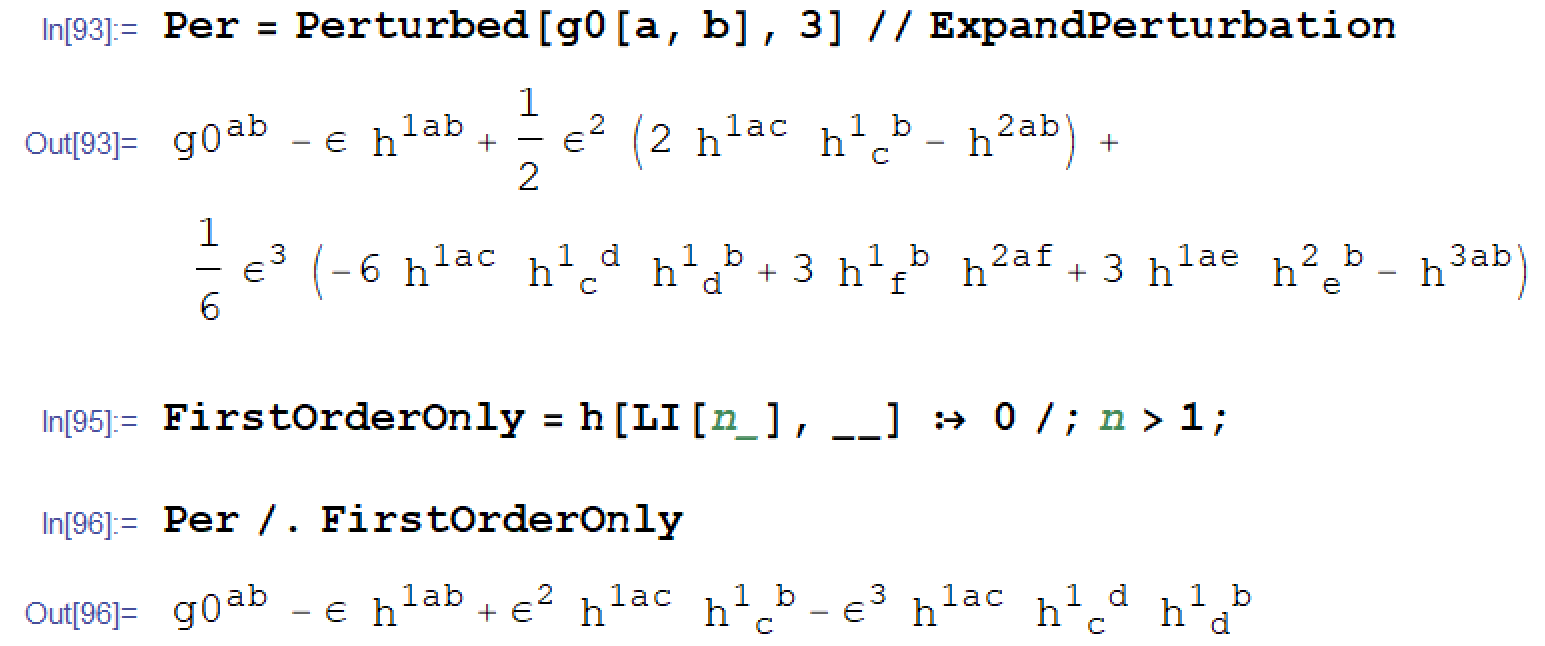
\includegraphics[scale=0.25]{first-order}
\end{figure}



By setting $\epsilon = 1$ we get the desired expansion above. Presumably we should be able to get expansions to very orders of $h$ this way. Let's try order 5:
\begin{figure}[!htb]
	\centering
	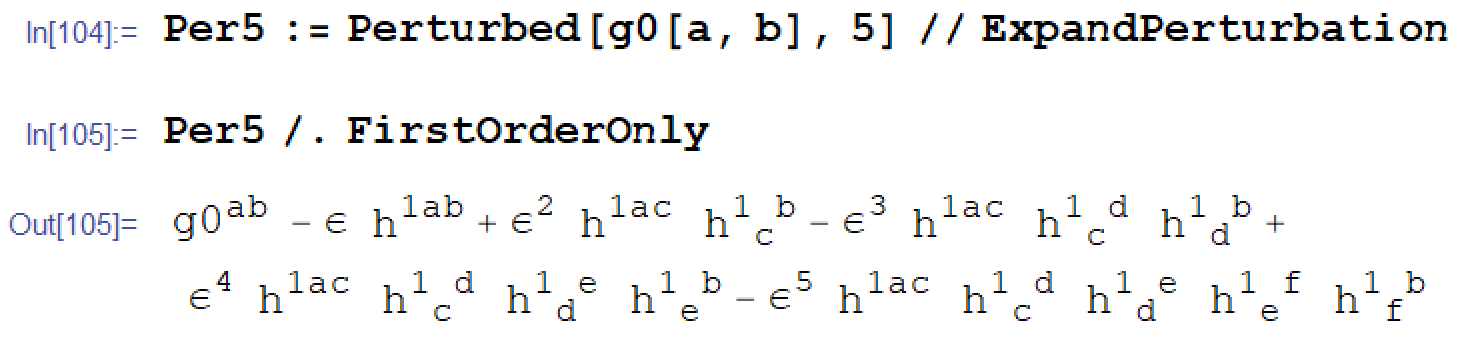
\includegraphics[scale=0.25]{order5}
\end{figure}

in more readable symbols:
\begin{align}
g^{\mu\nu} = g^{(0)\mu\nu} -h^{ab} + h^{ac}\tensor{h}{_c^b} - h^{ac}\tensor{h}{_c^d}\tensor{h}{_d^b} + h^{ac}\tensor{h}{_c^d}\tensor{h}{_d^e}\tensor{h}{_e^b} - h^{ac}\tensor{h}{_c^d}\tensor{h}{_d^e}\tensor{h}{_e^f}\tensor{h}{_f^b} + \dots
\end{align}

We also need to expand the determinant. Hinterbichler says:
\begin{align}
\boxed{\sqrt{-g} = \sqrt{-g^{(0)}}\lb 1 + \f{1}{2}h - \f{1}{4}\lp h^{\mu\nu}h_{\mu\nu} - \f{1}{2}h^2 \rp + \dots \rb}
\end{align}
but I will need to reproduce this somehow, by hand or by xACT. (\textbf{Exercise})\\

We also have the following useful identity:
\begin{align}
\boxed{\langle h^n \rangle = \sum^\infty_{l=0}(-1)^l {{l+n-1}\choose{l}} [h^{l+n}]}
\end{align}
for writing the determinant of $g_{\mu\nu}$ as an expansion in $h_{\mu\nu}$. 






\newpage
\subsubsection{Spherical solutions and the Vainshtein radius}

Next, we look at static spherical solutions. Let $D=4$, and for definiteness we pick the action
\begin{align}
{S = \f{1}{2\kappa^2}\int d^Dx\, \lb \sqrt{-g}R - \sqrt{-g^{(0)}}\f{1}{4}m^2 g^{(0)\mu\alpha}g^{(0)\nu\beta}\lp h_{\mu\nu}h_{\alpha\beta} - h_{\mu\alpha}h_{\nu\beta} \rp \rb}
\end{align}
where the mass term is minimal. We will attempt to find spherically symmetric solutions to the equation of motion
\begin{align}
{0 = \sqrt{-g}\lp R^{\mu\nu} - \f{1}{2}Rg^{\mu\nu} \rp + \sqrt{-g^{(0)}}\f{m^2}{2}\lp g^{(0)\mu\alpha}g^{(0)\nu\beta}h_{\alpha\beta} - g^{(0)\alpha\beta}h_{\alpha\beta}g^{(0)\mu\nu}\rp}
\end{align} 
which we took for granted (good to check/reproduce). We will also assume that the absolute metric is Minkowskian:
\begin{align}
g^{(0)}_{\mu\nu}dx^\mu dx^\nu = -dt^2 + dr^2 + r^2 d\Omega^2
\end{align}
where we're using the $(-,+,+,+)$ convention. We thus consider a spherically symmetric solution (hopefully a good ansatz) whose line element is
\begin{align}
g_{\mu\nu}dx^\mu dx^\nu = -B(r)dt^2 + C(r)dr^2+ A(r)r^2d\Omega^2.
\end{align}
Here we're of course assuming (and hoping) that our ansatz works and is diagonal, or else we will get mixed $r,t,\Omega$ terms in the line element. \\

Next, we recall the identity:
\begin{align}
[F(r)\delta_{ij} + G(r)x_ix_j]dx^idx^j = [F(r) + r^2 G(r)]dr^2 + F(r)r^2d\Omega^2.
\end{align}
Based on the ansatz, we have the following:
\begin{align}
&A(r) \equiv F(r)\nn\\
&C(r) \equiv F(r) + r^2 G(r)
\end{align}
Now, we recall from last time where we found a spherical solution to the easier problem involving $h_{\mu\nu}$. We started with the matrix elements $h_{00}$, $h_{0i}$, and $h_{ij}$ and expressed these in terms of the appropriate $F(r), G(r), -B(r)$. Here we're doing kind of the reverse process where we're starting with the spherical ansatz. Now, we wish to use the equations of motion to write down the relationship among these spherical solutions $F(r), G(r), -B(r)$. How do we do this?\\

Since we've assumed the solution is diagonal, we can rely on the $tt,rr$, and $\theta\theta \equiv \phi\phi$ equations of motion. In order to get the desired results in the end, we can set
\begin{align}
&g_{00}(r) = -B(r)\nn\\
&g_{0i}(r) = 0\nn\\
&g_{ij}(r) = A(r)\delta_{ij} + G(r)x_ix_j 
\end{align}
and define 
\begin{align}
C(r) \equiv A(r) + r^2 G(r).
\end{align}
As matrices:
\begin{align}
\boxed{[g_{\mu\nu}]_{\text{Cartesian}} = \begin{pmatrix}
	-B(r) &&&\\
	&A(r) + x^2G(r)&xyG(r)&xzG(r)\\
	&yxG(r)&A(r)+ y^2G(r)&yzG(r)\\
	&zxG(r)&zyG(r)&A(r)+ z^2G(r)
	\end{pmatrix}}
\end{align}
and
\begin{align}
[g^{(0)}_{\mu\nu}]_{\text{Spherical}} = \begin{pmatrix}
-1 &&&\\
&1& & \\
&&r^2&\\
&&&r^2 \sin^2\theta \end{pmatrix}
\end{align}
We start by evaluating $\sqrt{-g}$. This can be done in Mathematica:
\begin{lstlisting}
In[2]:= Det[{{-B, 0, 0, 0},
{0, A + x^2*G, x*y*G, x*z*G},
{0, y*x*G, A + y^2*G, y*z*G},
{0, z*x*G, z*y*G, A + z^2*G}}]

Out[2]= -B (A^3 + A^2 G x^2 + A^2 G y^2 + A^2 G z^2)
\end{lstlisting}
The output says the determinant of the $[g_{\mu\nu}]$ matrix is 
\begin{align}
-B(r)A^2(r)\lb A + \underbrace{(x^2 + y^2 + z^2)}_{r^2}G(r) \rb = -A^2B\underbrace{(A+r^2G)}_{C(r)} = -A^2BC.  
\end{align}
So, ${\sqrt{-g} = \sqrt{A^2BC}}$.  Next, we want to evaluate $\sqrt{-g^{(0)}}$. However, note that $[g_{\mu\nu}^{(0)}]$ is in spherical coordinates, while $[g_{\mu\nu}]$ is in Cartesian coordinates. We wish to be consistent, so we will just evaluate $\sqrt{-g^{(0)}}$ ``by analogy'' by reading off the numbers from the line element. Because
\begin{align}
g^{(0)}_{\mu\nu}dx^\mu dx^\nu &= -dt^2 + dr^2 + r^2 d\Omega^2 \nn\\
&= -(1)dt^2 + \lp 1 + 0 r^2 \rp dr^2 + (1)r^2d\Omega^2\nn\\
\text{and }  g_{\mu\nu}dx^\mu dx^\nu &= -B(r)dt^2 + C(r)dr^2+ A(r)r^2d\Omega^2\nn\\
&= -B(r)dt^2 + \lp A(r) + G(r) r^2 \rp dr^2+ A(r)r^2d\Omega^2
\end{align}
and because $\sqrt{-g} = \sqrt{A^2BC}$, we just have $\sqrt{-g^{(0)}} = \sqrt{-1} = 1$, in Cartesian coordinates, as expected. We're also writing the line element wrt $g^{(0)}$ like above so that it resembles the form of $[g_{\mu\nu}]$:
\begin{align}
\boxed{[g^{(0)}_{\mu\nu}]_{\text{Cartesian}} = \begin{pmatrix}
	-1 &&&\\
	&1 + 0x^2&0xy&0xz\\
	&0yx&1+0y^2&0yz\\
	&0zx&0zy&1+0z^2
	\end{pmatrix} = \begin{pmatrix}
	-1 &&&\\
	&1&&\\
	&&1&\\
	&&&1
	\end{pmatrix}}
\end{align}
which is also expected. Throughout the derivations, we will be using the boxed matrices as our metrics, both of which are in Cartesian coordinates. \\

With this, we first consider the $tt$ equation:
\begin{align}
{0 = \sqrt{-g}\lp R^{00} - \f{1}{2}Rg^{00} \rp + \sqrt{-g^{(0)}}\f{m^2}{2}\lp g^{(0)0\alpha}g^{(0)0\beta}h_{\alpha\beta} - g^{(0)\alpha\beta}h_{\alpha\beta}g^{(0)00}\rp}
\end{align}
We will unpack the second term first. Recall that
\begin{align}
h_{\mu\nu} = g_{\mu\nu} - g_{\mu\nu}^{(0)}.
\end{align}
So
\begin{align}
g^{(0)0\alpha}g^{(0)0\beta}h_{\alpha\beta} &= g^{(0)0\alpha}g^{(0)0\beta}\lp g_{\al\be} - g_{\al\be}^{(0)} \rp\nn\\
&= \underbrace{g^{(0)00}g^{(0)00}}_{1}\lp g_{00} - g_{00}^{(0)} \rp\nn\\
&= -B(r) + 1,
\end{align}
and
\begin{align}
g^{(0)\alpha\beta}h_{\alpha\beta}g^{(0)00} &= g^{(0)\alpha\beta}g^{(0)00}\lp g_{\al\be} - g_{\al\be}^{(0)}  \rp\nn\\
&= \sum^4_{\alpha=0}\lb g^{(0)\alpha\al}g^{(0)00}\lp g_{\al\al} - g_{\al\al}^{(0)}  \rp  \rb\nn\\
&= \lp-B+1\rp  - \lp A + x^2G -1  \rp -  \lp A + y^2G - 1 \rp - \lp A + z^2G - 1 \rp\nn\\
&= (-B+1) - (3A + r^2G -3).
\end{align}
And so we have successfully dealt with the second term:
\begin{align}
&\sqrt{-g^{(0)}}\f{m^2}{2}\lp g^{(0)0\alpha}g^{(0)0\beta}h_{\alpha\beta} - g^{(0)\alpha\beta}h_{\alpha\beta}g^{(0)00}\rp\nn\\
= &\,\f{m^2}{2}\lb (-B + 1) - (-B+1) - (3A + r^2G-3) \rb\nn\\
= &\,\f{m^2}{2}(-3A - r^2G + 3) \nn\\
= &\,\f{m^2}{2}\lp -3A + 3 - r^2 \f{C-A}{r^2}\rp\nn\\
= &\,\boxed{\f{m^2}{2}\lp  2A + C - 3\rp}
\end{align}
Now comes the difficult part of unpacking the Ricci tensor and scalar. We wish to evaluate the term
\begin{align}
R^{00} - \f{1}{2}Rg^{00}
\end{align}
for $\mu = \nu = 0$. First, $g^{00} = -1/B$ trivially. But what about $R^{00}$ and $R$? We will rely on Mathematica. Part of the calculations is done based on the Mathematica code provided by \href{https://arxiv.org/pdf/0904.4184.pdf}{\underline{Catalogue of Spacetimes}}. \\

\href{https://huanqbui.com/LaTeX projects/HuanBui_QM/Cartesian_Vainshtein.nb}{\underline{Here}} is the link to the notebook, which contains just the calculations for the $tt$ equation. There will be another notebook with the spherical calculations for the other $rr,\theta\theta\equiv \phi\phi$ equations as well. \textit{I'm writing this from the future... the solution below is found using Cartesian coordinates instead of spherical. While it is correct (and I have checked many times to make sure it was correct) it is very, very, cumbersome. The new notebook contains the spherical calculations for this $tt$ equation as well. If the reader is curious and wants to download a notebook to view the calculations, I recommend downloading the other notebook, link in the section where we derive the $rr$-equation.} The notebook requires no additional packages. It should run on any basic Mathematica installation. \\

We first clear some symbols, define the dimensions, metric, etc:
\begin{lstlisting}
Clear[coord, metric, inversemetric, affine, t, x, y, z]

r := Sqrt[x^2 + y^2 + z^2]

n := 4

coord := {t, x, y, z}

metric := {{-B[r], 0, 0, 0},
{0, A[r]+x^2*(-A[r]+C[r])/r^2, x*y*(-A[r]+C[r])/r^2, x*z*(-A[r] + C[r])/r^2},
{0, y*x*(-A[r]+C[r])/r^2, A[r]+y^2*(-A[r]+C[r])/r^2, y*z*(-A[r] + C[r])/r^2},
{0, z*x*(-A[r]+C[r])/r^2, z*y*(-A[r]+C[r])/r^2, A[r] + z^2*(-A[r]+C[r])/r^2}}
\end{lstlisting}
Note that the metric $g_{\mu\nu}$ we should be using here must be in terms of $B(r), A(r), C(r)$, since we ultimately want solutions in terms of these functions. In matrix form, $[g_{\mu\nu}]$ is
\begin{align}
\boxed{[g_{\mu\nu}] = \begin{pmatrix}
	-B &&&\\
	&A + x^2\lp \f{C-A}{r^2} \rp&xy\lp \f{C-A}{r^2} \rp&xz\lp \f{C-A}{r^2} \rp\\
	&yx\lp \f{C-A}{r^2} \rp&A+ y^2\lp \f{C-A}{r^2} \rp&yz\lp \f{C-A}{r^2} \rp\\
	&zx\lp \f{C-A}{r^2} \rp&zy\lp \f{C-A}{r^2} \rp&A+ z^2\lp \f{C-A}{r^2} \rp
	\end{pmatrix}}
\end{align}
It is easy to check that $\sqrt{-g} = \sqrt{A^2BC}$ by brute forcing in Mathematica. I won't reproduce the results here. \\

Next, we find the inverse metric, in order to set up for calculations of Christoffel symbols, Riemann, Ricci tensors, and the Ricci scalar. 
\begin{lstlisting}
inversemetric := Simplify[Inverse[metric]]
\end{lstlisting}
Every now and then, we define ``rules''  to force-simplify things. \\

Next, we calculate Christoffel symbols of the 2nd kind:
\begin{lstlisting}

Calculating the Christoffel symbols of the second kind: 

rule1 = {A[Sqrt[
x^2 + y^2 + z^2]] + (x^2 + y^2 + z^2) G[Sqrt[
x^2 + y^2 + z^2]] -> C[r]};

affine := affine = 
Simplify[Table[(1/2) Sum[
inversemetric[[Mu, Rho]] (D[metric[[Rho, Nu]], coord[[Lambda]]] + 
D[metric[[Rho, Lambda]], coord[[Nu]]] - 
D[metric[[Nu, Lambda]], coord[[Rho]]]), {Rho, 1, n}], {Nu, 1, 
n}, {Lambda, 1, n}, {Mu, 1, n}]]

listaffine := 
Table[If[UnsameQ[affine[[Nu, Lambda, Mu]], 
0], {Style[
Subsuperscript[\[CapitalGamma], Row[{coord[[Nu]], coord[[Lambda]]}], 
coord[[Mu]]], 18], "=", Style[affine[[Nu, Lambda, Mu]], 14]}], {Lambda, 
1, n}, {Nu, 1, Lambda}, {Mu, 1, n}]

Simplify[TableForm[Partition[DeleteCases[Flatten[listaffine], Null], 3], 
TableSpacing -> {1, 2}] /. rule1]
\end{lstlisting}

This outputs an entire table of nontrivial Christoffel symbols which we won't worry about. Here's a snippet of the output:
\begin{figure}[!htb]
	\centering
	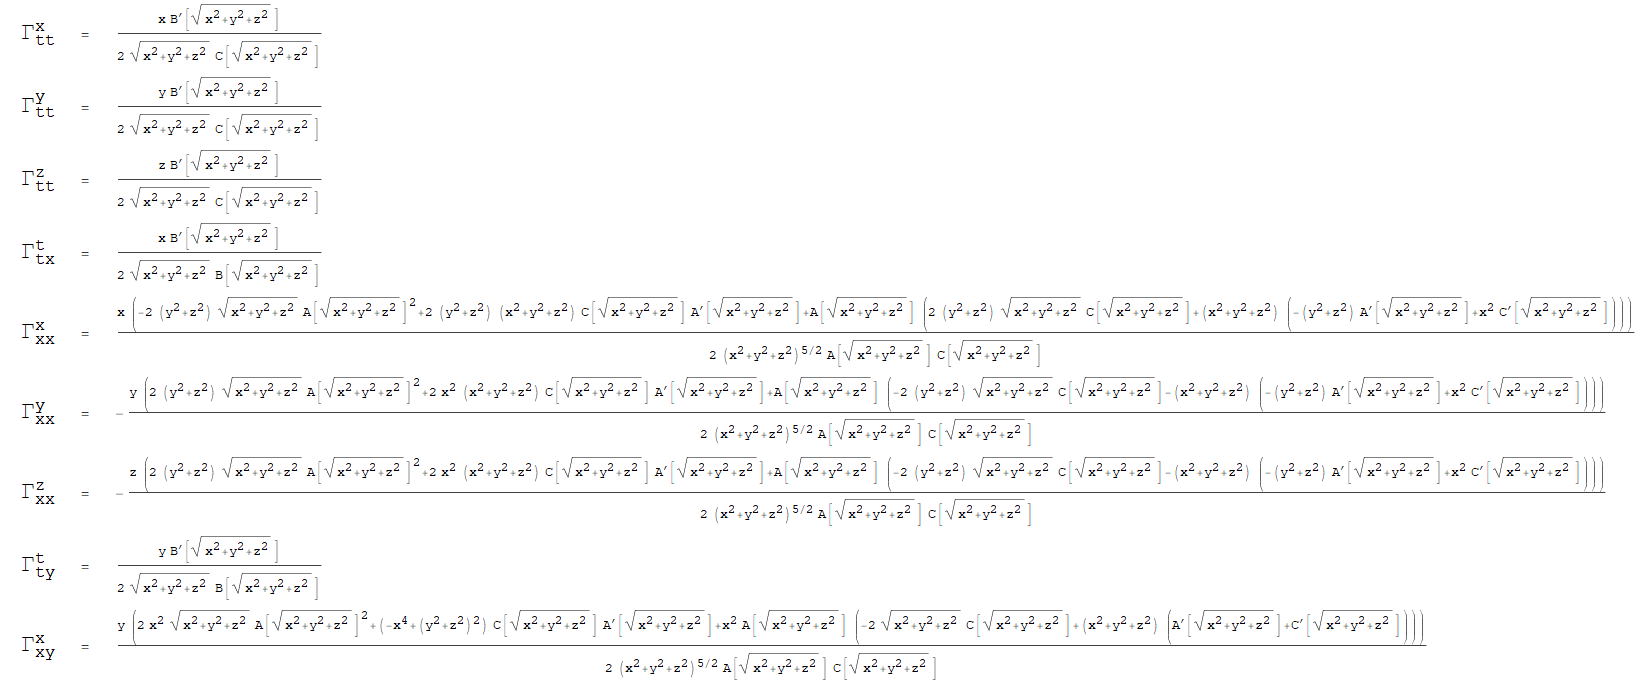
\includegraphics[scale=0.3]{christoffel}
\end{figure}

Next, we define and compute the lower-index Riemann tensors:
\begin{lstlisting}
Defining the Riemann tensor.

riemann := 
riemann = Table[
D[affine[[Nu, Sigma, Mu]], coord[[Rho]]] - 
D[affine[[Nu, Rho, Mu]], coord[[Sigma]]] + 
Sum[affine[[Rho, Lambda, Mu]] affine[[Nu, Sigma, Lambda]] - 
affine[[Sigma, Lambda, Mu]] affine[[Nu, Rho, Lambda]], {Lambda, 1, 
n}], {Mu, 1, n}, {Nu, 1, n}, {Rho, 1, n}, {Sigma, 1, n}]



Defining the Riemann tensor with lower indices.

riemannDn := 
riemannDn = 
Table[Simplify[
Sum[metric[[Mu, Kappa]] riemann[[Kappa, Nu, Rho, Sigma]], {Kappa, 1, 
n}]], {Mu, 1, n}, {Nu, 1, n}, {Rho, 1, n}, {Sigma, 1, n}]

listRiemann := 
Table[If[UnsameQ[riemannDn[[Mu, Nu, Rho, Sigma]], 
0], {Style[
Subscript[R, 
Row[{coord[[Mu]], coord[[Nu]], coord[[Rho]], coord[[Sigma]]}]], 16], 
"=", riemannDn[[Mu, Nu, Rho, Sigma]]}], {Nu, 1, n}, {Mu, 1, Nu}, {Sigma, 
1, n}, {Rho, 1, Sigma}]

Simplify[Simplify[
TableForm[Partition[DeleteCases[Flatten[listRiemann], Null], 3], 
TableSpacing -> {2, 2}] /. rule1] /. rule1]
\end{lstlisting}

There are (obviously) a lot of them. Here are some:
\begin{figure}[!htb]
	\centering
	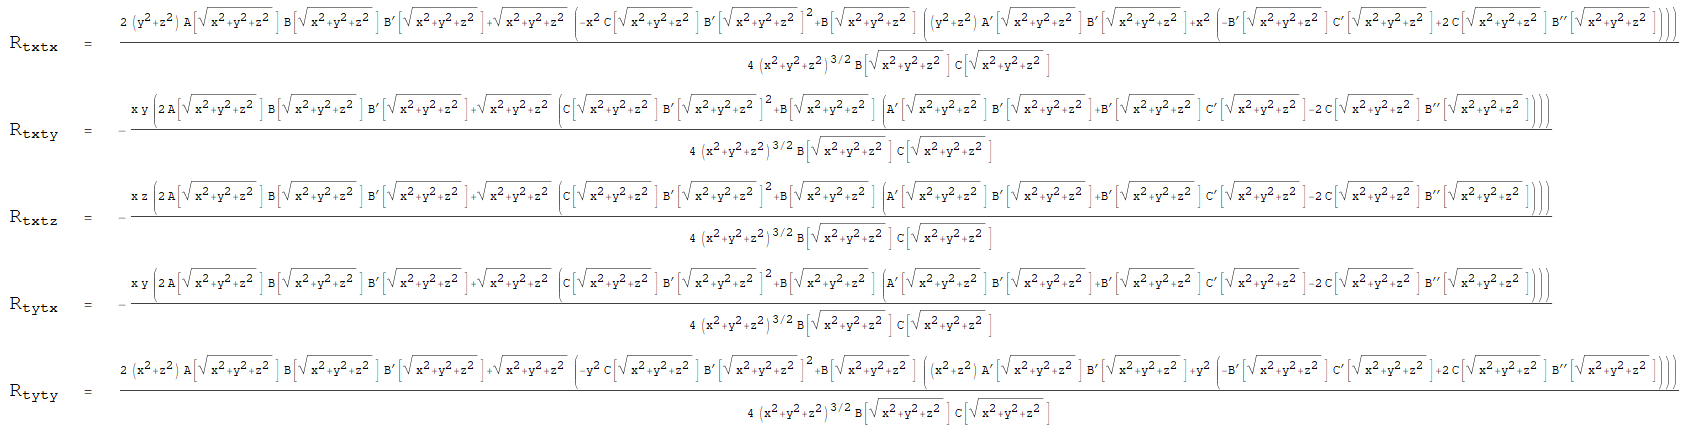
\includegraphics[scale=0.25]{riemann}
\end{figure}

Almost there... Next, we define the Ricci tensors:
\begin{lstlisting}
Defining Ricci tensor:

ricci := ricci = 
Table[Simplify[Sum[riemann[[Rho, Mu, Rho, Nu]], {Rho, 1, n}]], {Mu, 1, 
n}, {Nu, 1, n}]

listRicci := 
Table[If[UnsameQ[ricci[[Mu, Nu]], 
0], {Style[Subscript[R, Row[{coord[[Mu]], coord[[Nu]]}]], 16], "=", 
Style[ricci[[Mu, Nu]], 16]}], {Nu, 1, 4}, {Mu, 1, Nu}]

TableForm[Partition[DeleteCases[Flatten[listRicci], Null], 3], 
TableSpacing -> {1, 2}]
\end{lstlisting}
There aren't too many of these, but no expression is short enough to fit the width of the page, so I will just include $R_{tt}$ and truncated versions of $R_{xx}, R_{yy},\dots$
\begin{figure}[!htb]
	\centering
	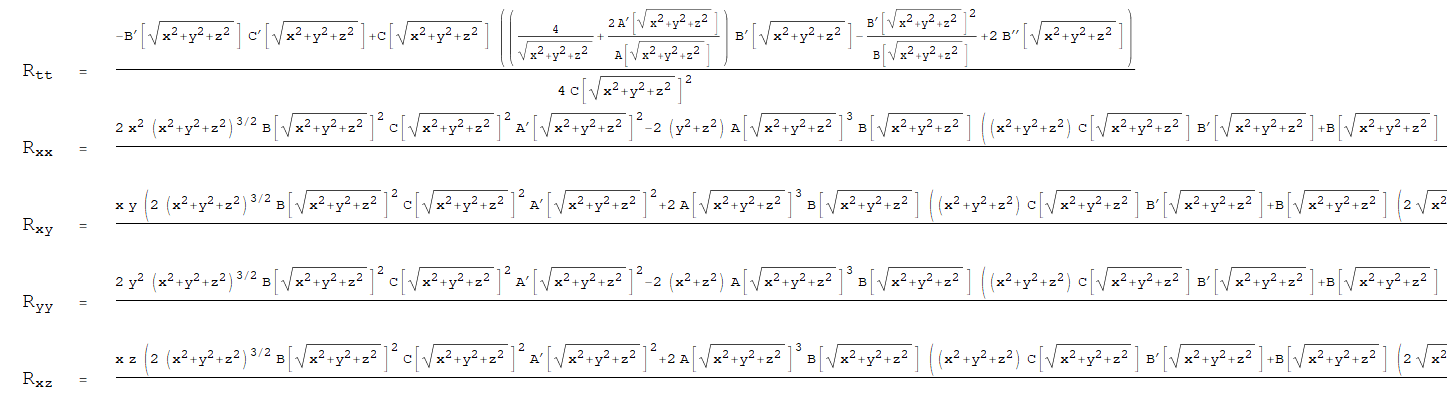
\includegraphics[scale=0.3]{riccitensors}
\end{figure}

Okay. Moving on to the last item: the Ricci scalar.
\begin{lstlisting}
Defining Ricci scalar:

ricciscalar := 
ricciscalar = 
Simplify[Sum[
Sum[inversemetric[[Mu, Nu]] ricci[[Nu, Mu]], {Mu, 1, n}], {Nu, 1, n}]]

Simplify[Simplify[ricciscalar]]
\end{lstlisting}
The output isn't very useful to work with:
\begin{figure}[!htb]
	\centering
	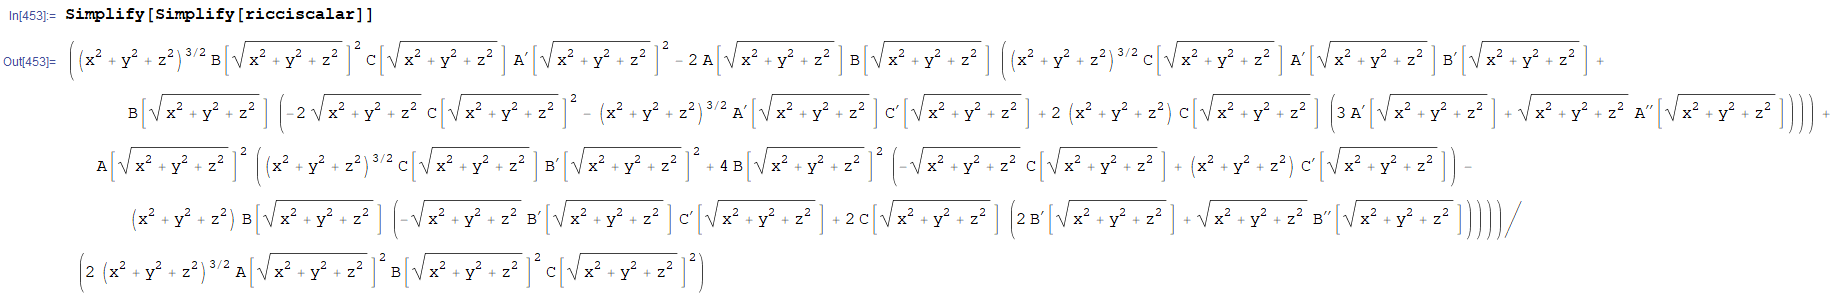
\includegraphics[scale=0.25]{ricciscalar}
\end{figure}
so we will define more rules to simplify it to a useful form:
\begin{lstlisting}
rule2 = {Sqrt[x^2 + y^2 + z^2] -> R};

rule3 = {(x^2 + y^2 + z^2)^(-1/2) -> R^(-1)};

rule4 = {(x^2 + y^2 + z^2)^(3/2) -> R^3};

rule5 = {(x^2 + y^2 + z^2) -> R^2};

rule6 = {Sqrt[R^2]^(-1) -> R^(-1)};

RR = Simplify[
Simplify[Simplify[
Simplify[
Simplify[
Simplify[Simplify[ricciscalar] /. rule1] /. rule2] /. 
rule3] /. rule4] /. rule5] /. rule6]

(1/(2 R^2 A[R]^2 B[R]^2 C[
R]^2))(R^2 B[R]^2 C[R] Derivative[1][A][R]^2 + 
2 A[R] B[R] (-R^2 C[R] Derivative[1][A][R] Derivative[1][B][R] + 
B[R] (2 C[R]^2 + R^2 Derivative[1][A][R] Derivative[1][C][R] - 
2 R C[R] (3 Derivative[1][A][R] + 
R (A^\[Prime]\[Prime])[R]))) + 
A[R]^2 (R^2 C[R] Derivative[1][B][R]^2 - 
4 B[R]^2 (C[R] - R Derivative[1][C][R]) + 
R B[R] (R Derivative[1][B][R] Derivative[1][C][R] - 
2 C[R] (2 Derivative[1][B][R] + R (B^\[Prime]\[Prime])[R]))))
\end{lstlisting}
In symbols:
\begin{figure}[!htb]
	\centering
	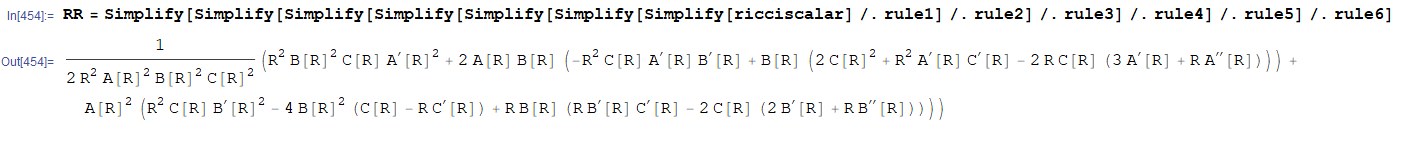
\includegraphics[scale=0.32]{ricciscalar1}
\end{figure}

Now, we want the quantity, which is LeftTerm minus RightTerm
\begin{align}
R^{00} - \f{1}{2}Rg^{00} \equiv \text{LeftTerm} - \text{RightTerm}. 
\end{align}
The \textbf{LeftTerm} is obtained from raising the indices of $R_{\mu\nu}$. This turned out not to be very difficult, because $g^{0\nu}$ entries are all zero except at $\nu = 0$ where $g^{00} = -1/B$. We need two of these to raise the indices of $R_{\mu\nu}$, so as a result we have $R^{00} = (1/B^2)R_{00}$. The \textbf{Rtt} term in the code below is just $R^{00}$.

\begin{lstlisting}
LeftTerm := 
Simplify[Simplify[
Simplify[
Simplify[
Simplify[Simplify[Rtt /. rule1] /. rule2] /. rule3] /. 
rule4] /. rule5] /. rule6];

RightTerm := 
Simplify[Simplify[
Simplify[
Simplify[
Simplify[Simplify[(1/2)*RR*(-1/B[R]) /. rule1] /. rule2] /. 
rule3] /. rule4] /. rule5] /. rule6];

LeftTerm - RightTerm
\end{lstlisting} 

The \textbf{RightTerm} is just $(1/2)Rg^{00}$. The output is
\begin{figure}[!htb]
	\centering
	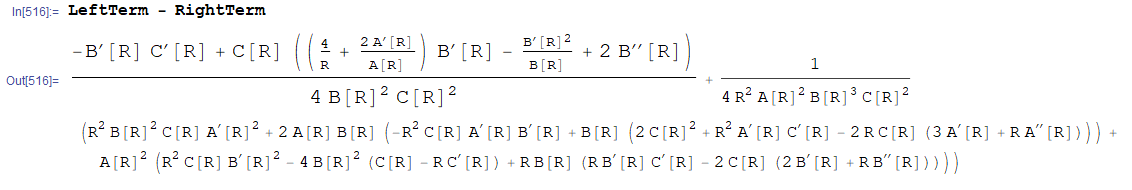
\includegraphics[scale=0.3]{leftright}
\end{figure}

Next, we define more rules to help with simplifying things:
\begin{lstlisting}
rule7 = {(2 C[R]^2 + R^2 Derivative[1][A][R] Derivative[1][C][R] - 
2 R C[R] (3 Derivative[1][A][R] + R (A^\[Prime]\[Prime])[R])) ->
STUFF1};

Simplify[LeftTerm - RightTerm /. rule7]

rule8 = {R^2 C[R] Derivative[1][A][R]^2 -> STUFF2};

Simplify[Simplify[LeftTerm - RightTerm /. rule7] /. rule8]

rule9 = {-4 A[R]^2 (C[R] - R Derivative[1][C][R]) -> STUFF3};

Simplify[Simplify[
Simplify[LeftTerm - RightTerm /. rule7] /. rule8] /. rule9]

rule10 = {2 STUFF1 A[R] -> STUFF4};

Simplify[Simplify[
Simplify[Simplify[LeftTerm - RightTerm /. rule7] /. rule8] /. 
rule9] /. rule10]

rule11 = {STUFF2 + STUFF3 + STUFF4 -> STUFF5};

Simplify[Simplify[
Simplify[
Simplify[Simplify[LeftTerm - RightTerm /. rule7] /. rule8] /. 
rule9] /. rule10] /. rule11]
\end{lstlisting}


We expand the final output and look for things to cancel:
\begin{lstlisting}

Simplify[Simplify[
Simplify[
Simplify[Simplify[LeftTerm - RightTerm /. rule7] /. rule8] /. 
rule9] /. rule10] /. rule11] // ExpandAll

\end{lstlisting}
\begin{figure}[!htb]
	\centering
	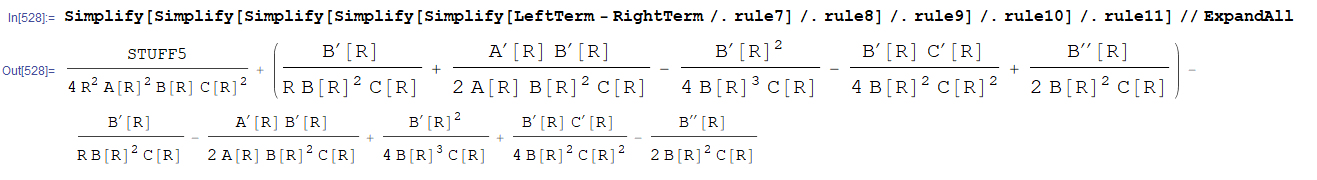
\includegraphics[scale=0.3]{outputt}
\end{figure}

Do you see where things cancel? \\
\begin{figure}[!htb]
	\centering
	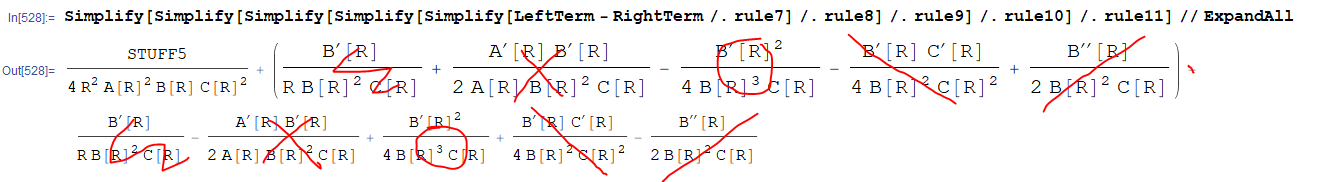
\includegraphics[scale=0.3]{outputtt}
\end{figure}




So we're left with just
\begin{align}
R^{00} - \f{1}{2}Rg^{00} = \f{r^2C(A')^2 - 4A^2(C-rC') + 2A\lp 2C^2+r^2A'C'-2r(3A'+rA'')C \rp}{4r^2A^2BC^2}.
\end{align}
Next, we bring in the square root of minus the determinant of $g$:
\begin{align}
&\sqrt{-g}\lp R^{00} - \f{1}{2}Rg^{00} \rp \nn\\
= &\sqrt{A^2BC} \f{r^2C(A')^2 - 4A^2(C-rC') + 2A\lp 2C^2+r^2A'C'-2r(3A'+rA'')C \rp}{4r^2A^2BC^2}.
\end{align}

And... we have the $tt$ equation:
\begin{align}
0 &= \sqrt{-g}\lp R^{00} - \f{1}{2}Rg^{00} \rp + \sqrt{-g^{(0)}}\f{m^2}{2}\lp g^{(0)00\al}g^{(0)0\be}h_{\al\be} - g^{(0)\al\be}h_{\al\be}g^{(0)00} \rp \nn\\
0 &= \sqrt{A^2BC}\lc{r^2C(A')^2 - 4A^2(C-rC') + 2A\lp 2C^2+r^2A'C'-2r(3A'+rA'')C \rp}\rc\nn\\
&\quad  + \f{m^2}{2}\lp  2A + C - 3\rp(4r^2A^2BC^2)
\end{align}
The simplified form, the \textbf{$tt$ equation} is:
\begin{empheq}[box=\widefbox]{align}
0 &=  4BC^2m^2r^2A^3 + [2B(C-3)C^2m^2r^2 - 4\sqrt{A^2BC}(C-rC')]A^2 \nn\\
&\quad\quad 2\sqrt{A^2BC}[2C^2-2r(3A'+rA'')C+r^2A'C']A + C\sqrt{A^2BC}r^2(A')^2
\end{empheq}

Next, we find the $rr$ equation. It is at this point that we realized we've been doing things the HARD WAY by working in Cartesian coordinates. There's a reason, however. In Cartesian coordinates, the determinant of $g_{\mu\nu}$ does not have dependence on $r$ and $\sin\theta$. In spherical coordinates, there is dependence on $\theta$, but I think that because the $\sin\theta$ term appears in both the determinant of the $g$ metric and the Minkowskian metric, we can just ignore it because the LHS must be zero.\\

In any case, we learned something by taking the Cartesian route. We will soon see how well-behaved things become once we go to spherical coordinates. I have uploaded a \href{https://huanqbui.com/LaTeX projects/HuanBui_QM/SphericalSolution_Vainshtein.nb}{\underline{new Mathematica notebook}} with the actual, full, spherical solution. This notebook contains the derivation of the $tt$ equation as well.  \\

From here on, we will be using metrics in spherical coordinates. From the specified line elements, the metrics are:
\begin{align}
\boxed{[g_{\mu\nu}] = \begin{pmatrix}
	-B &&&\\
	&C&&\\
	&&Ar^2&\\
	&&&Ar^2\sin^2\theta
	\end{pmatrix}}
\end{align}
and
\begin{align}
\boxed{[g^{(0)}_{\mu\nu}] = \begin{pmatrix}
	-1 &&&\\
	&1&&\\
	&&r^2&\\
	&&&r^2\sin^2\theta
	\end{pmatrix}}
\end{align}

Let us redefine everything in terms of spherical coordinates in the notebook and go over the calculations again. Trust me this will be quick.
\begin{lstlisting}
Clear[coord, metric, inversemetric, affine, t, r, \[Theta], \[Phi]]

n := 4

coord := {t, r, \[Theta], \[Phi]}

metric := {{-B[r], 0, 0, 0},
{0, C[r], 0, 0},
{0, 0, r^2*A[r], 0},
{0, 0, 0, r^2*Sin[\[Theta]]^2*A[r]}}

inversemetric := Simplify[Inverse[metric]]


Calculating the Christoffel symbols of the second kind: 

affine := affine = 
Simplify[Table[(1/2) Sum[
inversemetric[[Mu, Rho]] (D[metric[[Rho, Nu]], coord[[Lambda]]] + 
D[metric[[Rho, Lambda]], coord[[Nu]]] - 
D[metric[[Nu, Lambda]], coord[[Rho]]]), {Rho, 1, n}], {Nu, 1, 
n}, {Lambda, 1, n}, {Mu, 1, n}]]

listaffine := 
Table[If[UnsameQ[affine[[Nu, Lambda, Mu]], 
0], {Style[
Subsuperscript[\[CapitalGamma], Row[{coord[[Nu]], coord[[Lambda]]}], 
coord[[Mu]]], 18], "=", Style[affine[[Nu, Lambda, Mu]], 14]}], {Lambda, 
1, n}, {Nu, 1, Lambda}, {Mu, 1, n}]

Simplify[TableForm[Partition[DeleteCases[Flatten[listaffine], Null], 3], 
TableSpacing -> {1, 2}] /. rule1]
\end{lstlisting}


Here are the Christoffel symbols in spherical coordinates:
\begin{figure}[!htb]
	\centering
	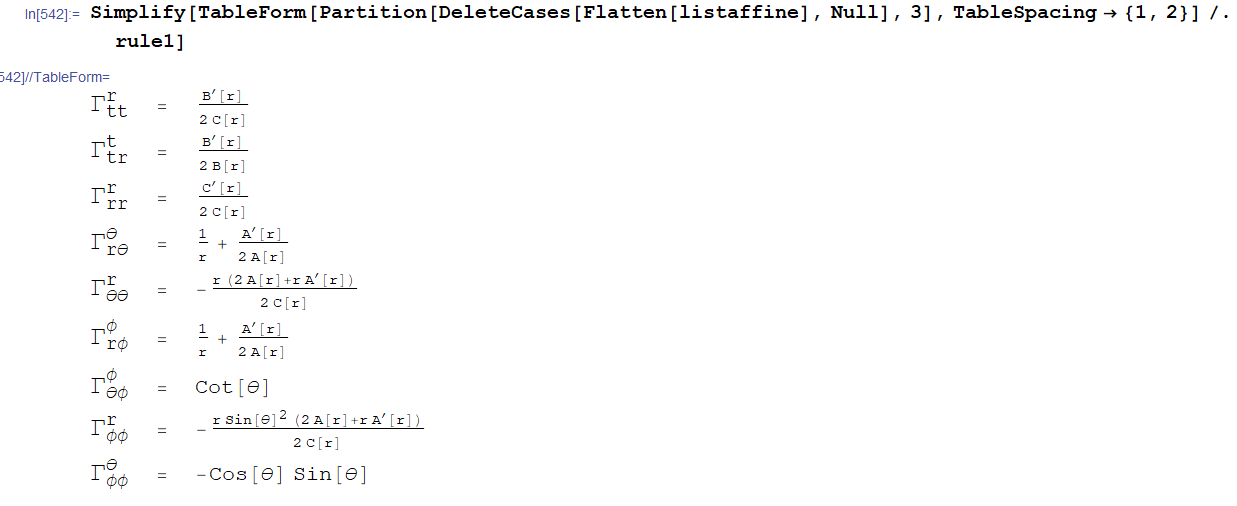
\includegraphics[scale=0.3]{sphericalchristoffel}
\end{figure}

Let the calculations continue...
\begin{lstlisting}
Defining the Riemann tensor.

riemann := 
riemann = Table[
D[affine[[Nu, Sigma, Mu]], coord[[Rho]]] - 
D[affine[[Nu, Rho, Mu]], coord[[Sigma]]] + 
Sum[affine[[Rho, Lambda, Mu]] affine[[Nu, Sigma, Lambda]] - 
affine[[Sigma, Lambda, Mu]] affine[[Nu, Rho, Lambda]], {Lambda, 1, 
n}], {Mu, 1, n}, {Nu, 1, n}, {Rho, 1, n}, {Sigma, 1, n}]



Defining the Riemann tensor with lower indices.

riemannDn := 
riemannDn = 
Table[Simplify[
Sum[metric[[Mu, Kappa]] riemann[[Kappa, Nu, Rho, Sigma]], {Kappa, 1, 
n}]], {Mu, 1, n}, {Nu, 1, n}, {Rho, 1, n}, {Sigma, 1, n}]

listRiemann := 
Table[If[UnsameQ[riemannDn[[Mu, Nu, Rho, Sigma]], 
0], {Style[
Subscript[R, 
Row[{coord[[Mu]], coord[[Nu]], coord[[Rho]], coord[[Sigma]]}]], 16], 
"=", riemannDn[[Mu, Nu, Rho, Sigma]]}], {Nu, 1, n}, {Mu, 1, Nu}, {Sigma, 
1, n}, {Rho, 1, Sigma}]

Simplify[Simplify[
TableForm[Partition[DeleteCases[Flatten[listRiemann], Null], 3], 
TableSpacing -> {2, 2}] /. rule1] /. rule1]
\end{lstlisting}

\begin{figure}[!htb]
	\centering
	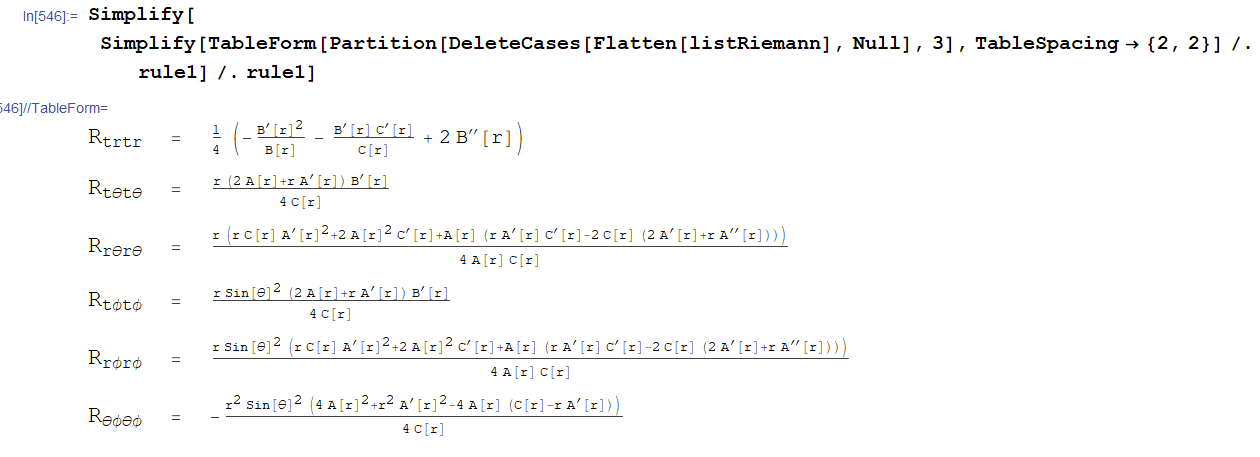
\includegraphics[scale=0.4]{sphericalriemann}
\end{figure}


Then comes the Ricci quantities:
\begin{lstlisting}
Defining Ricci tensor:

ricci := ricci = 
Table[Simplify[Sum[riemann[[Rho, Mu, Rho, Nu]], {Rho, 1, n}]], {Mu, 1, 
n}, {Nu, 1, n}]

listRicci := 
Table[If[UnsameQ[ricci[[Mu, Nu]], 
0], {Style[Subscript[R, Row[{coord[[Mu]], coord[[Nu]]}]], 16], "=", 
Style[ricci[[Mu, Nu]], 16]}], {Nu, 1, 4}, {Mu, 1, Nu}]

TableForm[Partition[DeleteCases[Flatten[listRicci], Null], 3], 
TableSpacing -> {1, 2}]

Defining Ricci scalar:

ricciscalar := 
ricciscalar = 
Simplify[Sum[
Sum[inversemetric[[Mu, Nu]] ricci[[Nu, Mu]], {Mu, 1, n}], {Nu, 1, n}]]

Simplify[Simplify[ricciscalar]]

RR = Simplify[ricciscalar]
\end{lstlisting}

Here's the output:
\begin{figure}[!htb]
	\centering
	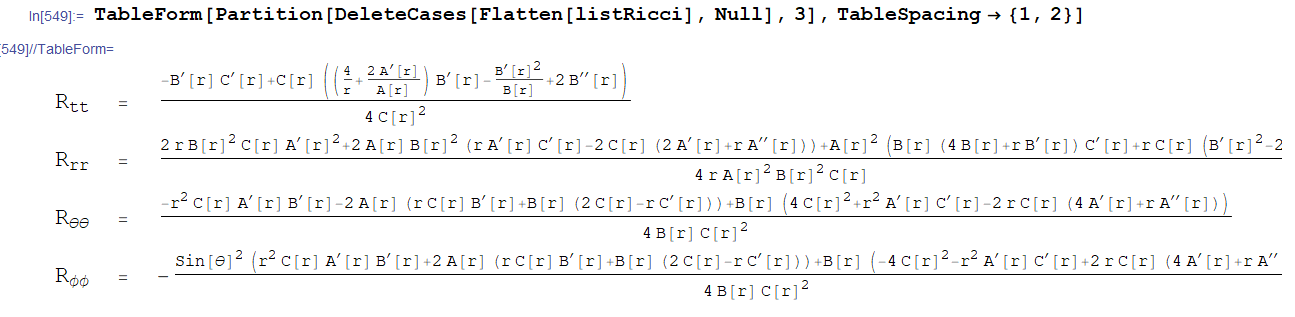
\includegraphics[scale=0.4]{sphericalricci}
	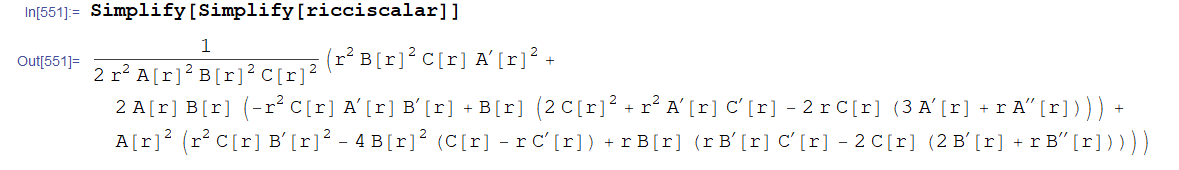
\includegraphics[scale=0.4]{sphericalricciscalar}
\end{figure}


Next we consider $R_{rr}$. We want $R^{rr}$, so we simply multiplying $R_{rr}$ by $1/C^2$, because $g_{\mu\nu}$ is diagonal in spherical coordinates. We first consider the term
\begin{align}
R^{rr} - \f{1}{2}Rg^{rr}.
\end{align}
To this end we repeat the process with the LeftTerm and RightTerm earlier to get
\begin{lstlisting}
LeftTerm := 
Simplify[Simplify[
Simplify[Simplify[Simplify[Simplify[Rrr/C[r]^2]]]]]];

RightTerm := 
Simplify[Simplify[
Simplify[Simplify[Simplify[Simplify[(1/2)*RR*(1/C[r])]]]]]];

Simplify[LeftTerm - RightTerm] // ExpandAll // ExpandAll
\end{lstlisting}
\begin{figure}[!htb]
	\centering
	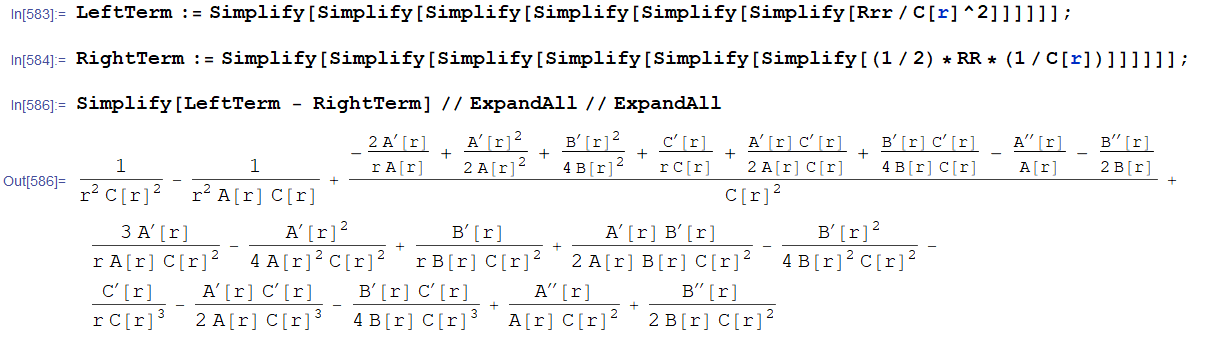
\includegraphics[scale=0.4]{sphericalleftright}
\end{figure}

Of course things cancel again!  Simplifying gives
\begin{figure}[!htb]
	\centering
	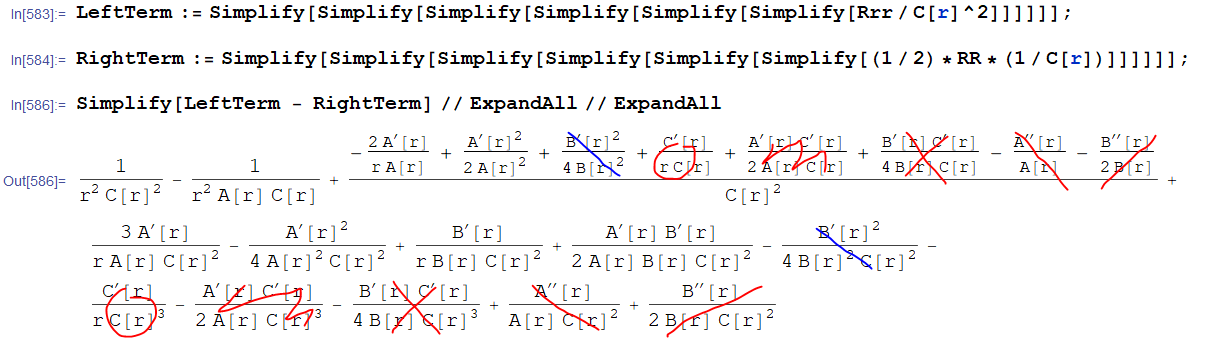
\includegraphics[scale=0.4]{sphericalleftrightcancel}
\end{figure}
\begin{figure}[!htb]
	\centering
	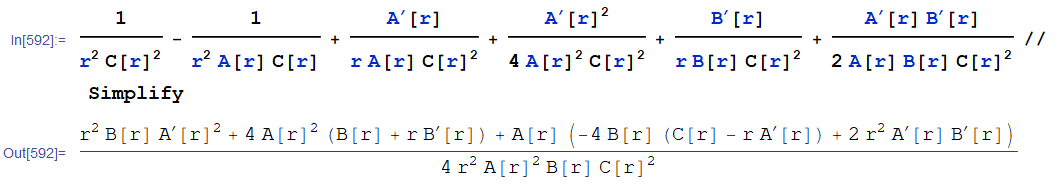
\includegraphics[scale=0.4]{simplified}
\end{figure}

\newpage

Next, we consider the term
\begin{align}
\sqrt{-g^{(0)}}\f{m^2}{2}\lp g^{(0)1\al}g^{(0)1\be}h_{\alpha\beta} - g^{(0)\al\be}h_{\al\be}g^{(0)11}  \rp.
\end{align}
Of course the first term is just going to be $h_{11} = C-1$. The second term has some contractions with factors of sines and $r^2$ floating around. But we can do this quickly by ignoring everything that is not the functions $A,B,C$. We can do this because when we multiplying the inverses $g^{(0)\mu\nu}$ with $h_{\mu\nu}$, the $r^2$ and sine factors automatically cancel out. The result is
\begin{align}
\sqrt{-g^{(0)}}\f{m^2}{2}\lp g^{(0)1\al}g^{(0)1\be}h_{\alpha\beta} - g^{(0)\al\be}h_{\al\be}g^{(0)11}  \rp &= \f{-m^2}{2}\lp 2(A-1) - (-B+1) \rp\nn\\
&= \boxed{\f{-m^2(2A+B-3)}{2}}
\end{align}
Putting everything together, we will find the $rr$ equation:
\begin{align}
0 &= \sqrt{-g}\lp R^{rr} - \f{1}{2}Rg^{rr} \rp + \sqrt{-g^{(0)}}\f{m^2}{2}\lp g^{(0)1\al}g^{(0)1\be}h_{\alpha\beta} - g^{(0)\al\be}h_{\al\be}g^{(0)11}  \rp\nn\\
0 &= \f{r^2B(A')^2 + 4A^2(B+rB') + A[-4B(C-rA')+2r^2A'B']}{A^2BC^2r^2}\nn\\
&\quad\quad - \f{2m^2(2A+B-3)}{\sqrt{A^2BC}}
\end{align}
Simplifying this gives the $rr$ equation:
\begin{empheq}[box=\widefbox]{align}
0 &= \f{4(B+rB')A^2 + [2r^2A'B'-4B(C-rA')]A + Br^2(A')^2 }{A^2BC^2r^2}\nn\\
&\quad\quad - \f{2(2A+B-3)m^2}{\sqrt{A^2BC}}
\end{empheq}

Finally, to get the $\theta\theta\equiv\phi\phi$ equation, we go through the process above once more. To make things a little easier, I'll just derive the $\theta\theta$ equation with $R_{\theta\theta}$ instead of $R^{\theta\theta}$. This way, I don't have to worry about factors of contractions, etc. 

\begin{figure}[!htb]
	\centering
	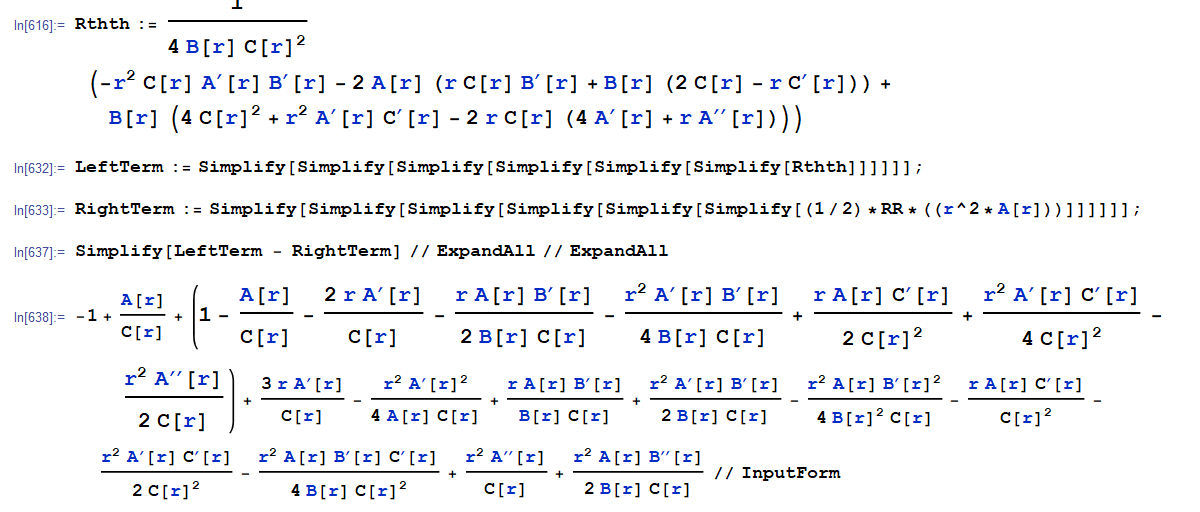
\includegraphics[scale=0.4]{theta}
\end{figure}
This simplifies to 
\begin{figure}[!htb]
	\centering
	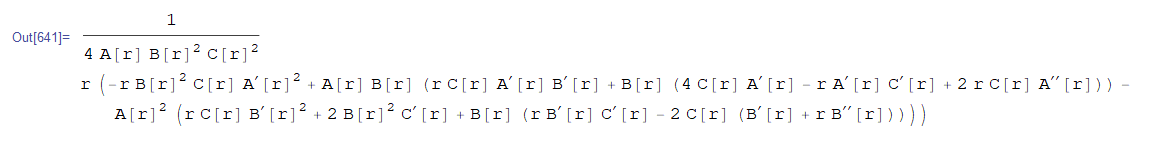
\includegraphics[scale=0.4]{thetasimplified}
\end{figure}


On to the $\sqrt{g^{(0)}}$ terms, we compute
\begin{align}
\sqrt{-g^{(0)}}\f{m^2}{2}\lp g^{(0)2\al}g^{(0)2\be}h_{\alpha\beta} - g^{(0)\al\be}h_{\al\be}g^{(0)22}  \rp.
\end{align}

I won't show the rest of the calculations here. The $\theta\theta\equiv \phi\phi$ equation is
\begin{empheq}[box=\widefbox]{align}
0 &= -2B^2C^2m^2rA^4 - 2B^2C^2(B+C-3)m^2rA^3\nn\\
& - \sqrt{A^2BC}\{2C'B^2 + [rB'C' - 2C(B'+rB'')]B + Cr(B')^2  \}A\nn\\
& +B\sqrt{A^2BC}[CrA'B'+B(4CA'-rC'A'+2CrA'')]A - B^2C\sqrt{A^2BC}r(A')^2.
\end{empheq}
I'll just put the other two equations here, for convenience. The $rr$ equation is
\begin{empheq}[box=\widefbox]{align}
0 &= \f{4(B+rB')A^2 + [2r^2A'B'-4B(C-rA')]A + Br^2(A')^2 }{A^2BC^2r^2}\nn\\
&\quad\quad - \f{2(2A+B-3)m^2}{\sqrt{A^2BC}}
\end{empheq}
The $tt$ equation is
\begin{empheq}[box=\widefbox]{align}
0 &=  4BC^2m^2r^2A^3 + [2B(C-3)C^2m^2r^2 - 4\sqrt{A^2BC}(C-rC')]A^2 \nn\\
&\quad\quad 2\sqrt{A^2BC}[2C^2-2r(3A'+rA'')C+r^2A'C']A + C\sqrt{A^2BC}r^2(A')^2
\end{empheq}


The next step is to solve for $A(r), B(r), C(r)$. To do this we first expand them in the flat space regime, where
\begin{align}
&B_0(r) = 1\\
&A_0(r) = 1\\
&C_0(r) = 1.
\end{align}
To obtain higher order terms, we introduce the expansion
\begin{align}
&B(r) = B_0(r) + \epsilon B_1(r) + \epsilon^2 B_2(r) + \dots\\
&C(r) = C_0(r) + \epsilon C_1(r) + \epsilon^2 C_2(r) + \dots\\
&A(r) = A_0(r) + \epsilon A_1(r) + \epsilon^2 A_2(r) + \dots
\end{align}
Plugging this into the equations we just found and collecting terms of $\mathcal{O}(\epsilon), \mathcal{O}(\epsilon^2),\dots$. This allows us to solve for $B_1,A_1,C_1$, then $B_2,A_2,C_2$, and so on. At $\mathcal{O}(\epsilon)$, we define the expansions in Mathematica only up to $\mathcal{O}(\epsilon)$. (Note: there are probably other ways to do this, but I like it this way. In addition, I will stop including the code because the notebook can be downloaded via the link above. I will just include important outputs from now on. )
\begin{figure}[!htb]
	\centering
	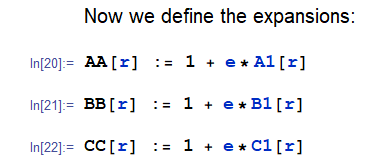
\includegraphics[scale=0.5]{expand}
\end{figure}
Next, we define the $tt,rr,\theta\theta$ equations, using these new function(al)s. (Again, there's probably a more clever and more efficient way to do this, but my method works so far so I'll stick with it.)  
\begin{figure}[!htb]
	\centering
	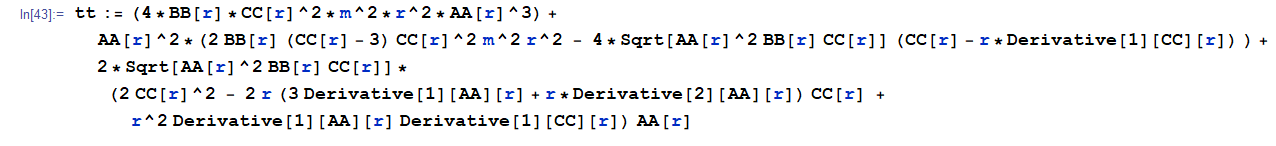
\includegraphics[scale=0.4]{tt}
	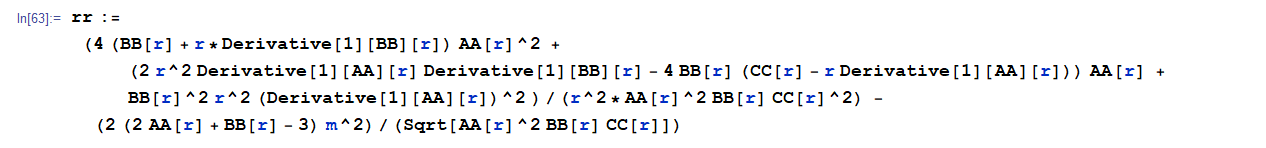
\includegraphics[scale=0.4]{rr}
	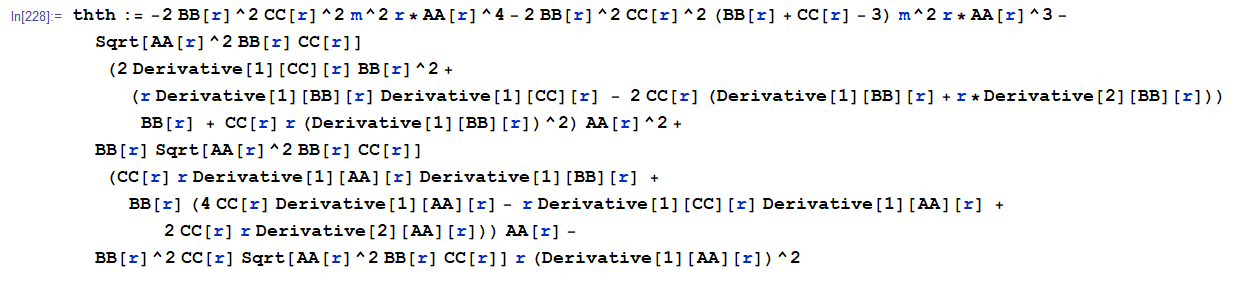
\includegraphics[scale=0.4]{thth}
\end{figure}
Once that is done, we must define some rules for simplification. Some of these rules are for helping Mathematica simplify, but some are also important when we extract out $\mathcal{O}(\epsilon)$ terms. 
\begin{lstlisting}
rule12 = {Sqrt[(1 + e A1[r])^2 (1 + e B1[r]) (1 + e C1[r])] -> 1};

rule13 = {Derivative[1][AA][r] -> e*Derivative[1][A1][r]};

rule14 = {(AA^\[Prime]\[Prime])[r] -> e*Derivative[2][A1][r]};

rule15 = {(CC^\[Prime]\[Prime])[r] -> e*Derivative[2][C1][r]};

rule16 = {Derivative[1][CC][r] -> e*Derivative[1][C1][r]};

rule17 = {Sqrt[(1 + e A1[r])^2 (1 + e B1[r]) (1 + e C1[r])]^(-1) -> 1};

rule18 = {(1 + e A1[r])^2 (1 + e B1[r]) (1 + e C1[r]) -> 1};

rule19 = {((1 + e A1[r])^2 (1 + e B1[r]) (1 + e C1[r])^2)^(-1) -> 1};

rule20 = {Derivative[1][BB][r] -> e*Derivative[1][B1][r]};

rule21 = {(BB^\[Prime]\[Prime])[r] -> e*Derivative[2][B1][r]};
\end{lstlisting}
With these rules, we proceed to collect the $\mathcal{O}(\epsilon)$ terms in each equation:
\begin{lstlisting}
ttSim := Coefficient[
tt /. rule12 /. rule13 /. rule14 /. rule15 /. rule16, e] // Simplify

rrSim := rr /. rule12 /. rule13 /. rule14 /. rule15 /. rule16 /. 
rule17 /. rule18 /. rule19 /. rule20 /. rule21

rrSimSim = 
Coefficient[rrSim /. rule12 /. rule13 /. rule14 /. rule15 /. rule16, 
e] // Simplify

ththSim := 
thth /. rule12 /. rule13 /. rule14 /. rule15 /. rule16 /. rule17 /. 
rule18 /. rule19 /. rule20 /. rule21

thSimSim = 
Coefficient[
ththSim /. rule12 /. rule13 /. rule14 /. rule15 /. rule16 /. 
rule17 /. rule18 /. rule19 /. rule20 /. rule21, e] // Simplify
\end{lstlisting}

Some equations are stubborn and require multiple simplifying, but the result is quite satisfying. Here are the coefficients of $\epsilon$ in the $tt,rr,\theta\theta$ equations, respectively:
\begin{figure}[!htb]
	\centering
	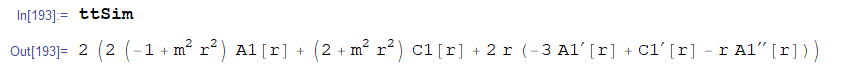
\includegraphics[scale=0.4]{e1}
	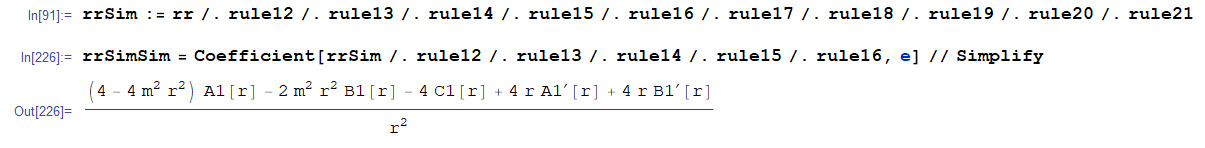
\includegraphics[scale=0.4]{e2}
	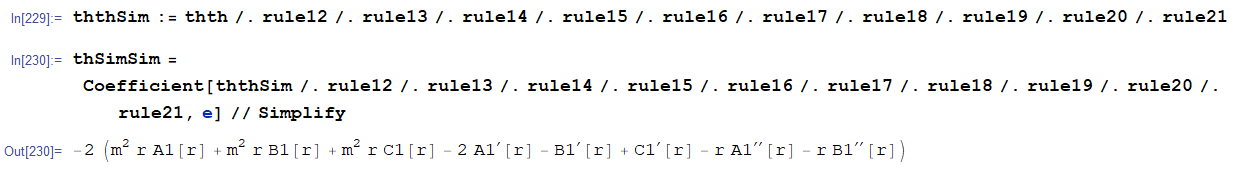
\includegraphics[scale=0.4]{e3}
\end{figure}
Now, these coefficients must all be zero when $A,B,C$ solve the $tt,rr,\theta\theta$ equations, so we have (in more readable symbols):
\begin{align}
&2(m^2r^2-1)A_1+(m^2r^2+2)C_1+2r(-3A_1'+C_1'-rA_1'')= 0\\
&\f{-1}{2}B_1m^2+\lp \f{1}{r^2}-m^2 \rp A_1 + \f{r(A_1'+B_1')-C_1}{r^2} = 0\\
&rA_1m^2+rB_1m^2+rC_1m^2-2A_1'-B_1'+C_1'-rA_1''-rB_1''=0
\end{align}
Okay. To solve for $A_1,B_1,C_1$, we start with simultaneously solving three equations algebraically for $A_1,A_1',A_1''$ in terms of $B,C$ are their derivatives. To do this, we use Mathematica's NSolve:
\begin{lstlisting}
NSolve[{ttSim == 0, rrSimSim == 0, thSimSim == 0}, {A1[r], 
Derivative[1][A1][r], Derivative[2][A1][r]}] // 
Simplify // FullSimplify
\end{lstlisting}
Here I'm storing the solutions in new variables for ease of access:
\begin{figure}[!htb]
	\centering
	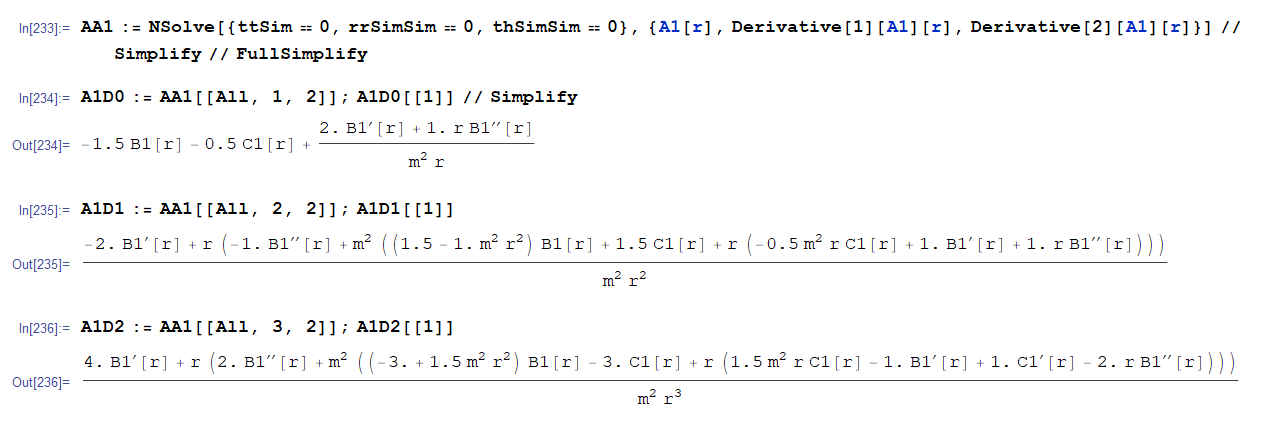
\includegraphics[scale=0.4]{AA}
\end{figure}
Once this is done, we write down two equations: (1) $A_1' = \p_r A_1$, and (2) $A_1''=\p_r A_1$, then proceed to algebraically solve this system for $C_1$ and $C_1'$ in terms of $B_1$ and its derivatives. I will only the include the input.
\begin{figure}[!htb]
	\centering
	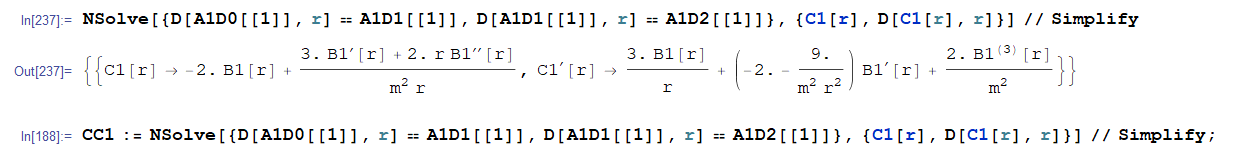
\includegraphics[scale=0.4]{CC}
\end{figure}
Finally, settings $C_1' - \p_r C_1 = 0$, we get a second-order differential equation for $B_1(r)$:
\begin{figure}[!htb]
	\centering
	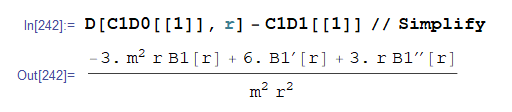
\includegraphics[scale=0.4]{BB}
\end{figure}
Of course this simplifies to 
\begin{align}
\boxed{-3rB_1m^2 + 6B_1' + 3rB_1'' = 0}
\end{align}
This can be DSolve'd easily in Mathematica:
\begin{lstlisting}
DSolve[-3 m^2 r B1[r] + 6 Derivative[1][B1][r] + 
3 r (B1^\[Prime]\[Prime])[r] == 0, B1[r], r]
\end{lstlisting}
which says
\begin{align}
B_1(r) = \mathfrak{C_1}\f{e^{-mr}}{r} + \mathfrak{C_2}\f{e^{mr}}{2mr}
\end{align}
where $\mathfrak{C_1}$ and $\mathfrak{C_2}$ are integration constants. Now, when $m\to 0$, $B_1(r)$ must remain finite, so we rule out the other linearly independent solution. This gives 
\begin{align}
{B_1(r) = -\f{8GM}{3}\f{e^{-mr}}{r}}
\end{align}
where the integration constant has been chosen so that we agree with the solution \eqref{mass} obtained from the Green's function. \\

From here, it is \textit{very easy} to get $C_1, A_1$ from $B_1$, because we already solved for these in terms of $B$ and $B,C$ respectively:
\begin{figure}[!htb]
	\centering
	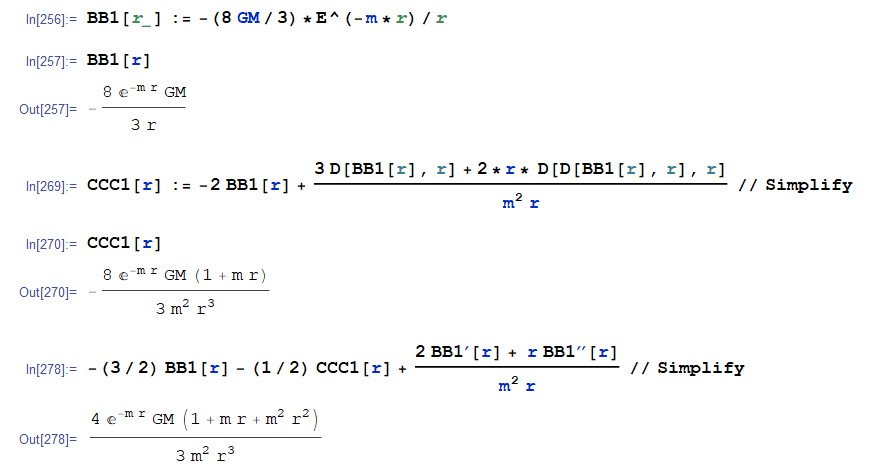
\includegraphics[scale=0.4]{ABC}
\end{figure}
\begin{empheq}[box=\widefbox]{align}
B_1(r) &= -\f{8GM}{3}\f{e^{-mr}}{r}\\
C_1(r) &= -\f{8GM}{3}\f{e^{-mr}}{r}\f{1+mr}{m^2r^2}\\
A_1(r) &= \f{4GM}{3}\f{e^{-mr}}{r}\f{1+mr+m^2r^2}{m^2r^2}
\end{empheq}

So, the $\mathcal{O}(\epsilon)$ problem is done, so we move on to the $\mathcal{O}(\epsilon^2)$ problem. The procedure will be exactly the same, so I will just put the code-outputs here without saying much. Some new rules will be defined along the way to help Mathematica with simplification. Also, so as not to completely ruin the previous code for the $\mathcal{O}(\epsilon)$ problem, I will be using slightly different names for some functions. Thanks to Hinterbichler himself, I will be using a different function, \texttt{SeriesCoefficient[ ]}, for expanding and collecting the $\mathcal{O}(\epsilon^2)$ terms. This is a better way to do things than using just the naive \texttt{Coefficient[..., $\epsilon^2$]} function. First, we redefine the expansions:
\begin{figure}[!htb]
	\centering
	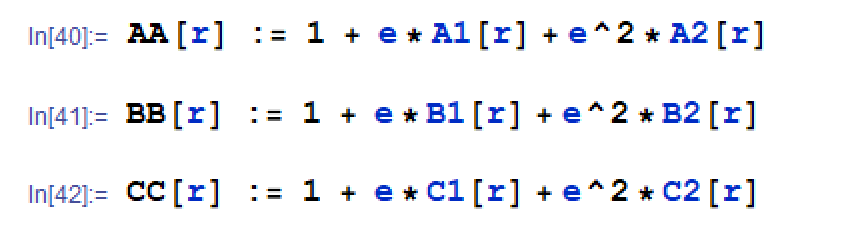
\includegraphics[scale=0.25]{expansions}
\end{figure}

Then we start with our original $tt$, $rr$, and $\theta\theta$ equations:
\begin{figure}[!htb]
	\centering
	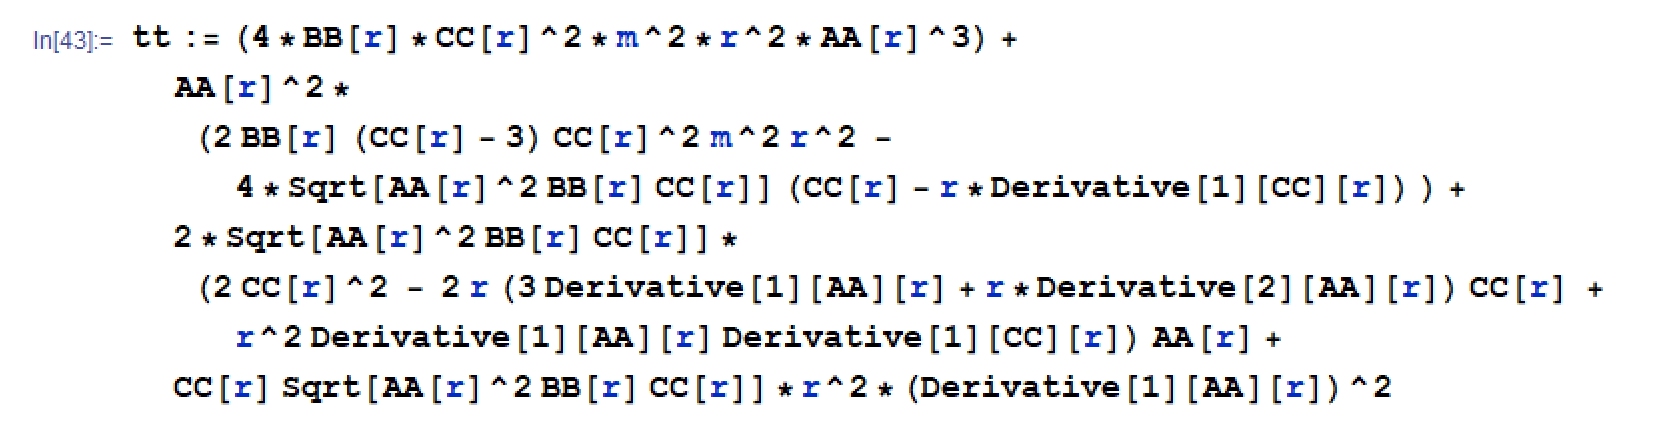
\includegraphics[scale=0.25]{tt2}
\end{figure}


\begin{figure}[!htb]
	\centering
	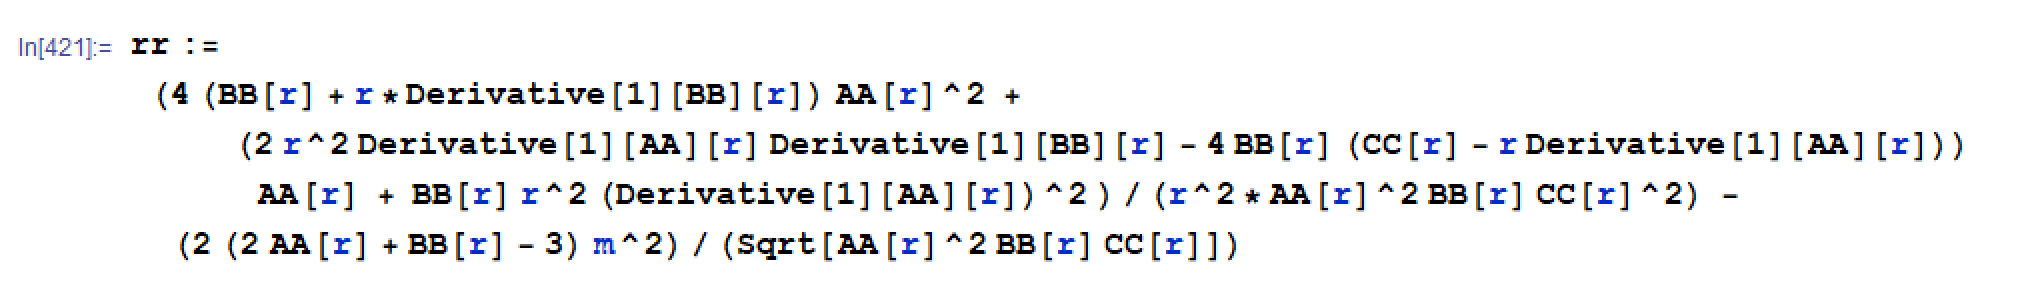
\includegraphics[scale=0.25]{rr2}
	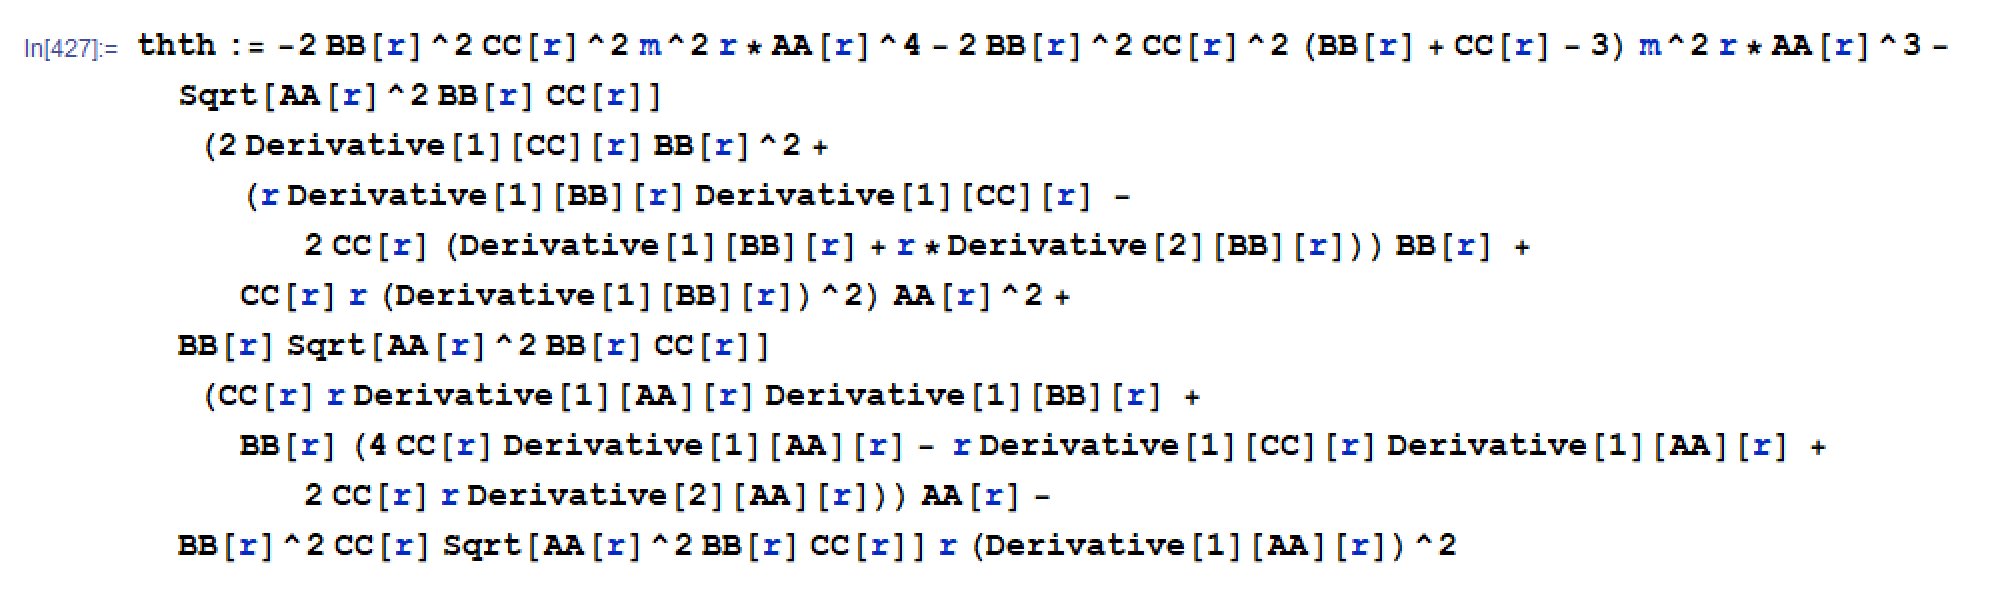
\includegraphics[scale=0.25]{thth2}
\end{figure}

To make Mathematica appropriately expand the series expansion of $B,C,A$ in these equations, we define 
\begin{figure}[!htb]
	\centering
	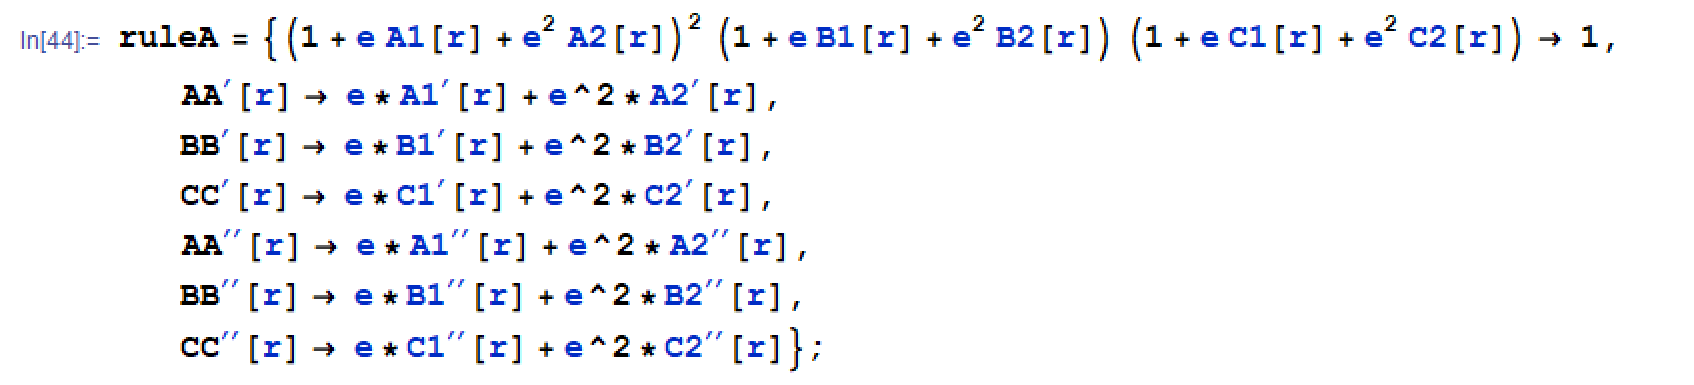
\includegraphics[scale=0.3]{ruleA}
\end{figure}\\



With this, the $tt$ equation, under the solved $B_1, C_1, A_1$ is given by
\begin{figure}[!htb]
	\centering
	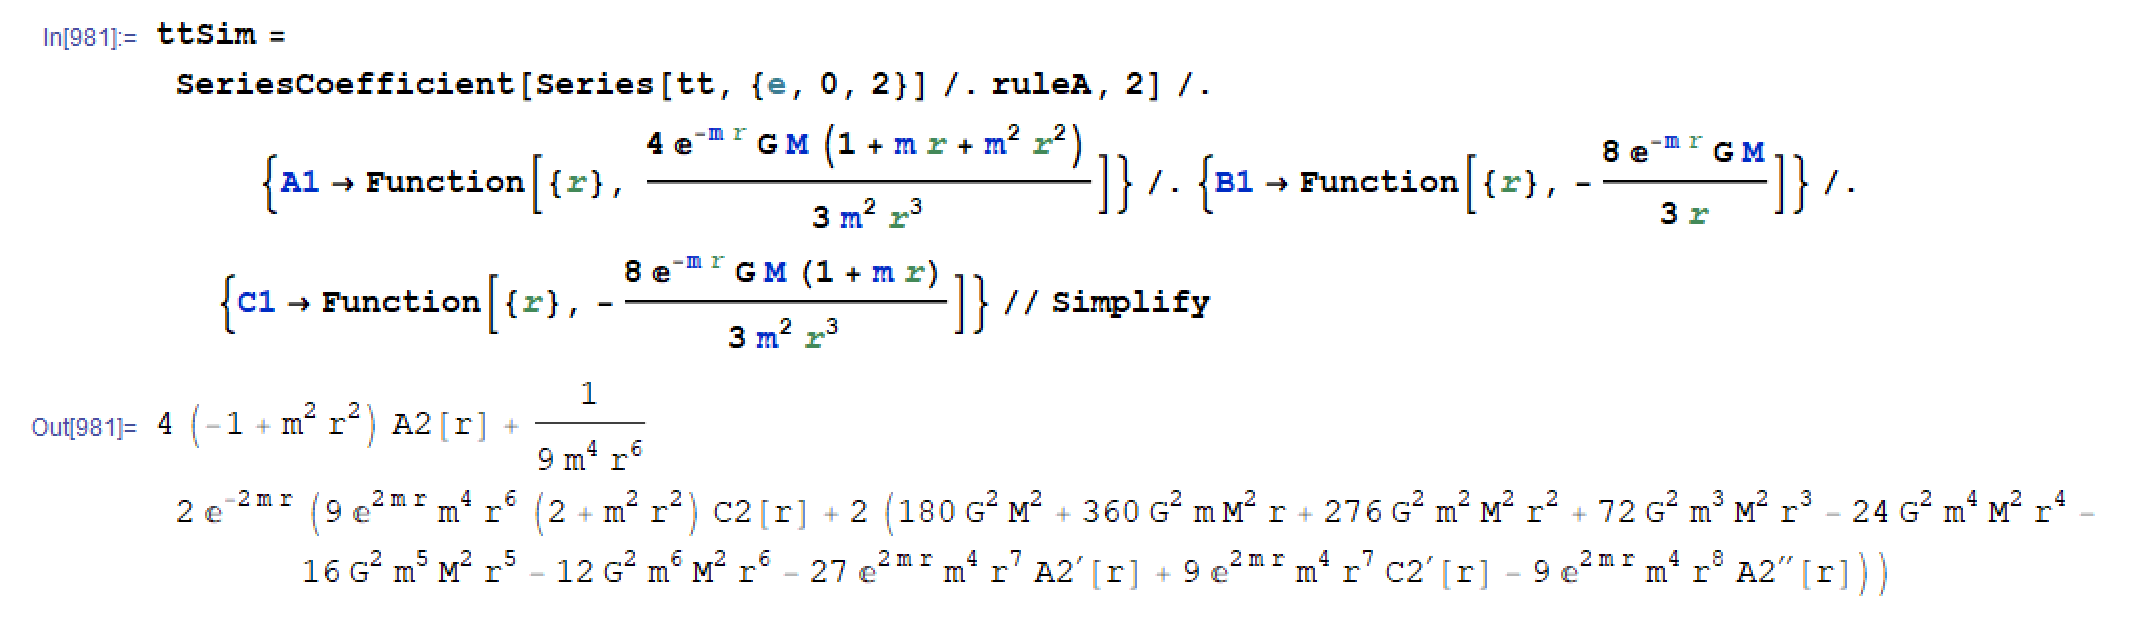
\includegraphics[scale=0.2]{tt2Sim}
\end{figure}\\




Notice that we're now using \texttt{SeriesCoefficient[]} instead of \texttt{Coefficient} like last time. We write
\begin{align}
0 = 
4 (-1 + m^2 r^2) A_2[r] +  \f{1}{9m^4r^6}
2 e^{-2 m r} \lb 9 e^{2 m r} m^4 r^6 (2 + m^2 r^2) C_2[r] + \right. \nn\\ 
\left.  2 \lp   180 G^2 M^2 + 360 G^2 m M^2 r + 276 G^2 m^2 M^2 r^2 + 
72 G^2 m^3 M^2 r^3\right. \right. \nn\\ 
\left. - 24 G^2 m^4 M^2 r^4 - 16 G^2 m^5 M^2 r^5 - 
12 G^2 m^6 M^2 r^6 \right.\nn\\
\left.  - 27 e^{2 m r} m^4 r^7 A_2'[r] + 
9 e^{2 m r} m^4 r^7 C_2'[r] - 
9 e^{2 m r} m^4 r^8 A_2''[r]    \rp \left.    \rb
\end{align}


We do a similar thing for the $rr$ equation:
\begin{figure}[!htb]
	\centering
	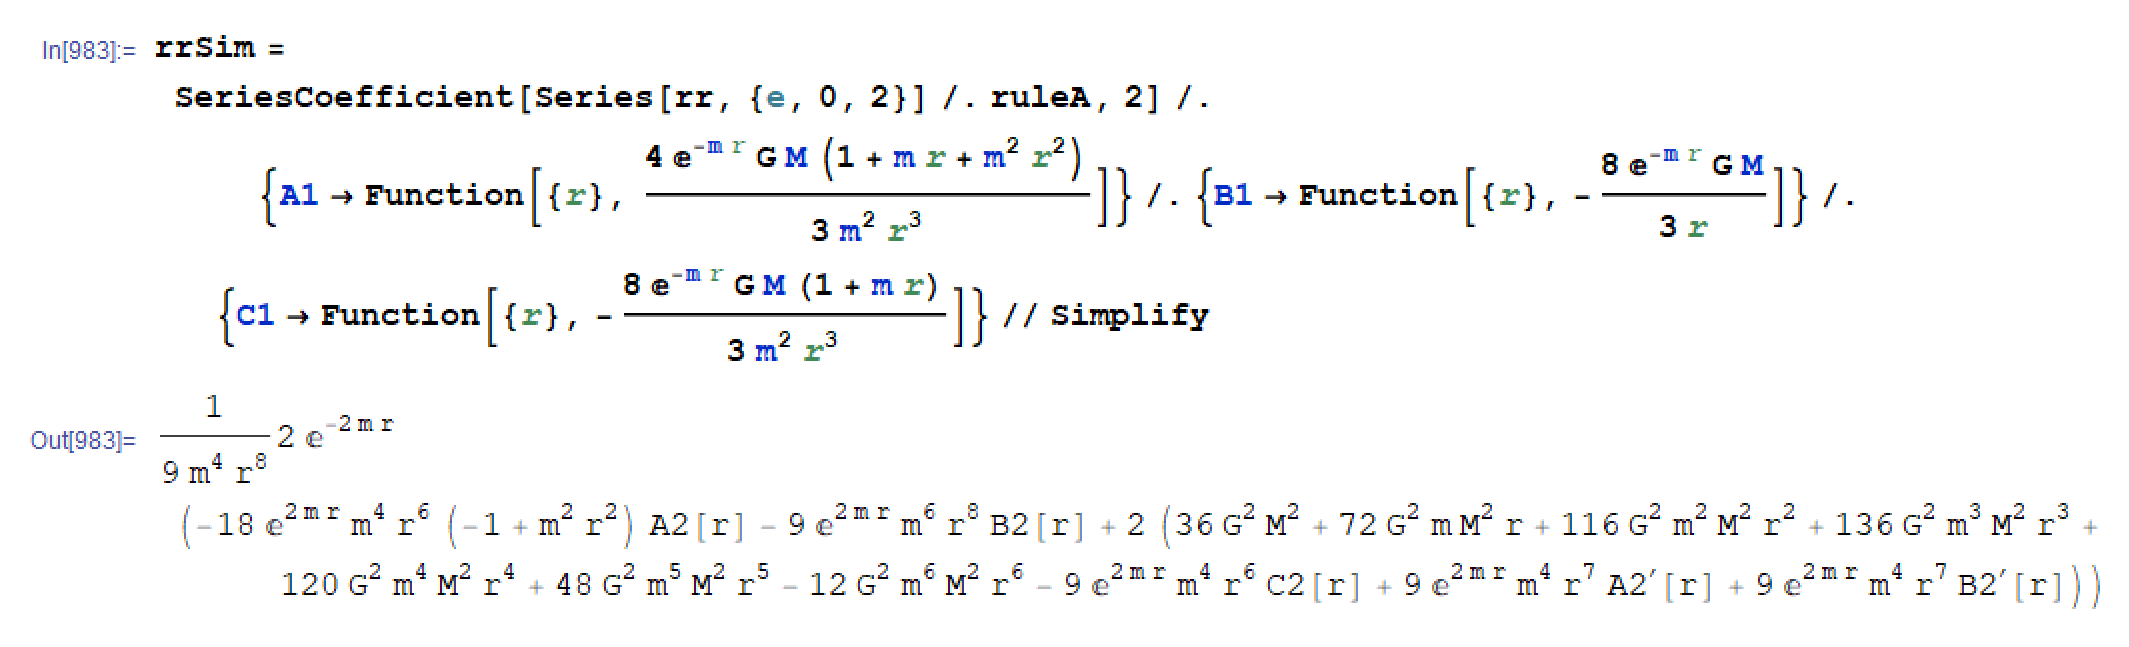
\includegraphics[scale=0.25]{rr2Sim}
\end{figure}
We write
\begin{align}
0 = \f{1}{9 m^4 r^8} 2 e^{-2 m r} \lb -18 e^{2 m r}
m^4 r^6 (-1 + m^2 r^2) A_2[r] - 9 e^{2 m r} m^6 r^8 B_2[r] \right.\nn\\ 
\left. + 
2 \lp 36 G^2 M^2 + 72 G^2 m M^2 r + 116 G^2 m^2 M^2 r^2 + 
136 G^2 m^3 M^2 r^3 \right. \right. \nn\\
\left. + 120 G^2 m^4 M^2 r^4 + 
48 G^2 m^5 M^2 r^5 - 12 G^2 m^6 M^2 r^6 \right.\nn\\
\left. -  9 e^{2 m r} m^4 r^6 C_2[r] + 
9 e^{2 m r} m^4 r^7 A_2'[r] + 
9 e^{2 m r} m^4 r^7 B_2'[r]\rp \left. \rb
\end{align}

Same thing for the $\theta\theta$ equation:
\begin{figure}[!htb]
	\centering
	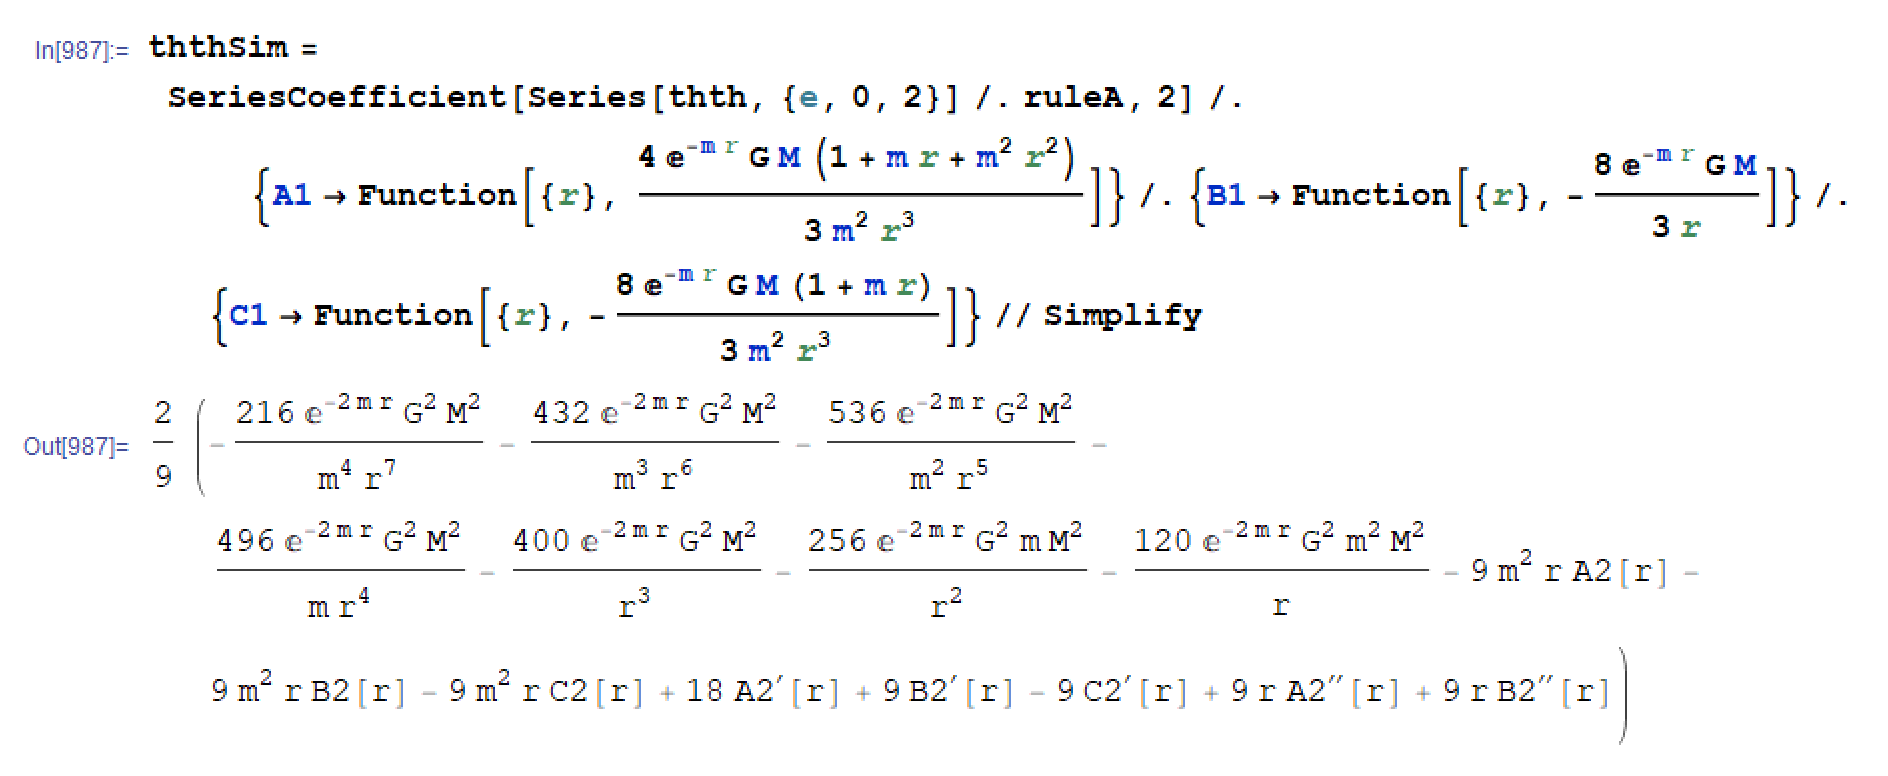
\includegraphics[scale=0.25]{thth2Sim}
\end{figure}
We write
\begin{align}
0 = \f{2}{9} \lb -\f{216e^{-2mr}G^2M^2}{m^4 r^7} 
-\f{432e^{-2mr}G^2M^2}{m^3 r^6}
-\f{536 e^{-2mr}G^2M^2}{m^2 r^5}
-\f{496 e^{-2mr}G^2M^2}{m r^4}  \right. \nn\\
\left. - \f{400 e^{-2 m r} G^2 M^2}{r^3} 
- \f{256 e^{-2 m r}G^2 m M^2}{r^2} 
- \f{120 e^{-2 m r} G^2 m^2 M^2}{r} - 9 m^2 r B_2[r] 
\right. \nn\\
\left. - 9 m^2 r A_2[r] - 9 m^2 r C_2[r] + 18 A_2'[r] + 9 B_2'[r] - 9 C_2'[r] + 9 r A_2''[r] + 9r B_2''[r] \rb 
\end{align}

Solving $tt=0, rr=0, \theta\theta = 0$ for $A_2, A_2', A_2''$ we get
\begin{figure}[!htb]
	\centering
	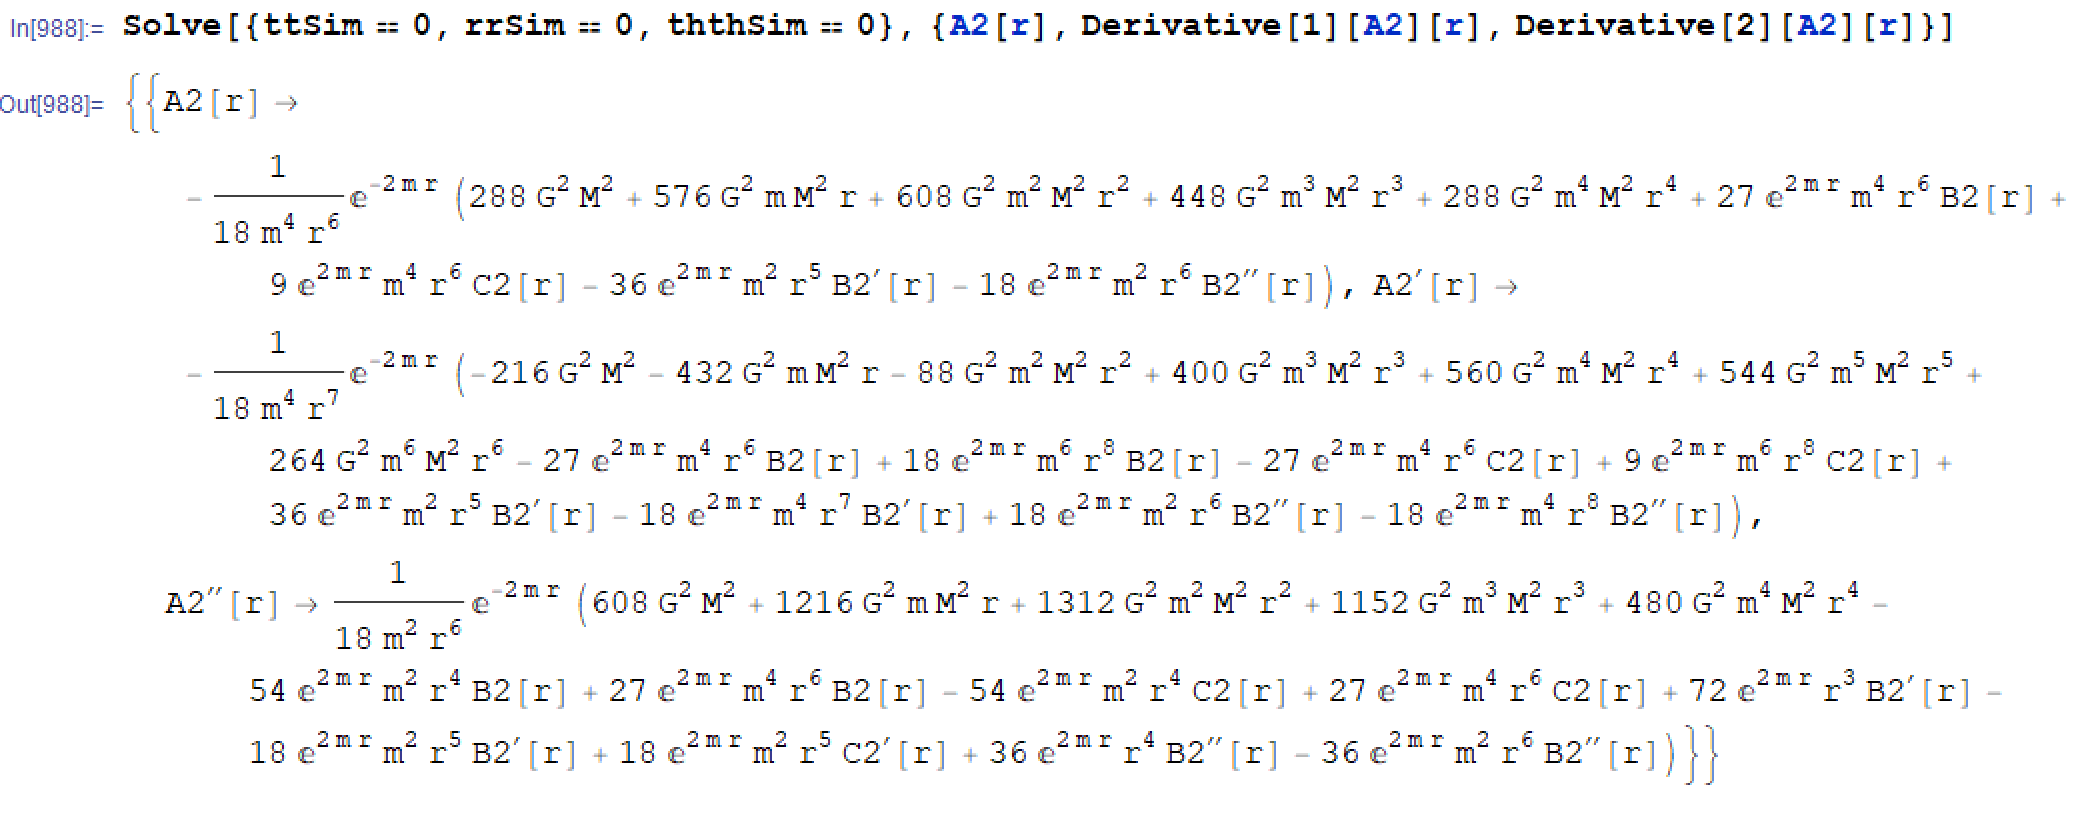
\includegraphics[scale=0.25]{A2}
	\includegraphics[scale=0.25]{A2bis}
\end{figure}\\


\newpage
Then we solve for $C_2, C_2'$ from the $A_2$ equations:
\begin{figure}[!htb]
	\centering
	\includegraphics[scale=0.2]{C2}
\end{figure}\\


Setting $C_2' = (\p_r)C_2$ we get the equation for $B_2$:
\begin{figure}[!htb]
	\centering
	\includegraphics[scale=0.17]{B2_new}
\end{figure}\\





We are only interested in the leading order term for $B_2$, we so find it. Plugging $B_2$ back into the $C_2$ and $A_2$ equations and taking their leading terms we get
\begin{figure}[!htb]
	\centering
	\includegraphics[scale=0.17]{A2B2C2}
\end{figure}\\



\newpage

With these, we set $\epsilon \to 1$ plug them back into the original expansion. After some factorizations we get
\begin{empheq}[box=\widefbox]{align}
B(r) &= 1 - \f{8}{3}\f{GM}{r}\lp 1 - \f{1}{6}\f{GM}{m^4r^5} + \dots\rp\nn\\
C(r) &= 1- \f{8}{3}\f{GM}{m^2r^3}\lp 1 - 14\f{GM}{m^4r^5} + \dots \rp\nn\\
A(r) &= 1 + \f{4}{3}\f{GM}{m^2r^3}\lp 1 - 4\f{GM}{m^4r^5} + \dots \rp
\end{empheq}

where the dots represent higher powers in the nonlinearity parameter $\epsilon$. The nonlinearity expansion is an expansion in the parameter $r_V/r$, with
\begin{align}
\boxed{r_V \equiv \lp \f{GM}{m^4} \rp^{1/5}}
\end{align}
is known as the \textbf{Vainshtein} radius. Notice that with this procedure, we can go on to extract solutions at $\mathcal{O}(\epsilon^n)$. However, we won't do that for now.\\







When $m\to 0$, $r_V \to \infty$, and hence the radius beyond which the solution can be trusted gets pushed out to infinity. Vainshtein argued (in 1972) that this perturbation expansion breaks down and says nothing about the true nonlinear behavior of masive gravity in the massless limit. Thus there was reason to hope that the vDVZ discontinuity was merely an artifact of linear perturbation theory, and that the true nonlinear solutions showed a smooth limit. 



\newpage
\subsubsection{Nonlinear Hamiltonian \& The Boulware-Deser mode}

We'll skip this section entirely. 










\newpage


\subsection{The Nonlinear St\"{u}ckelberg Formalism}


In this section we extend the St\"{u}ckelberg trick to full nonlinear order. This allows us to trace the breakdown in the linear expansion to strong coupling of the longitudinal mode. It also tells us about quantum corrections, the scale of the effective field theory and where it breaks down.  




\subsubsection{St\"{u}kelberg for gravity and the restoration of diffeomorphism invariance}


In this subsubsection we construct the full nonlinear gravitational St\"{u}ckelberg. The paper by Arkani-Hamed et. al. introduces this extensively. \\

The full finite gauge transformation for gravity is
\begin{align}
g_{\mu\nu}(x) \to \f{\p f^\al}{\p x^\mu} \f{\p f^\be}{\p x^\nu} g_{\al\be}(f(x))
\end{align}
where $f(x)$ is any arbitrary gauge function, which must be a diffeomorphism. In massive gravity, gauge invariance is broken only by the mass term. To restore invariance, we introduce a St\"{u}ckelberg field $Y^\mu(x)$ and apply it to the metric $g_{\mu\nu}$:
\begin{align}
\boxed{g_{\mu\nu}(x) \to G_{\mu\nu} = \f{\p Y^\al}{\p x^\mu} \f{\p Y^\be}{\p x^\nu} g_{\al\be}(Y(x))}
\end{align}

The Einstein-Hilbert term $\sqrt{-g}R$ does not change under this substitution, because it is gauge invariant. The substitution looks similar to a gauge transformation with gauge parameter $Y^\mu$, so no $Y$ fields are introduced into the Einstein-Hilbert part of the action.\\

The graviton mass term, however, picks up dependence on $Y's$ in such a way that it will not be invariant under the following gauge transformation:
\begin{align}
&g_{\mu\nu}(x)\to\f{\p f^\al}{\p x^\mu} \f{\p f^\be}{\p x^\nu} g_{\al\be}(f(x))\\
& Y^\mu(x) \to f^{-1}(Y(x))^\mu
\end{align}
with $f(x)$ being the gauge function. This is because the combination $G_{\mu\nu}$ is gauge invariance. To see this we transform $g_{\mu\nu}$:
\begin{align}\label{transf}
G_{\mu\nu} = \p_\mu Y^\al \p_\nu Y^\be g_{\al\be}(Y(x)) \to \p_\mu Y^\al \p_\nu Y^\be [???]
\end{align}
How does $g_{\al\be}(Y(x))$ transform under $f$? To correctly do this transformation, we can start with transforming something easy first, say the scalar field, $\phi$. We know that $\phi(x)$ transforms under $f$ as $\phi \to \phi(f(x))$. We wish to know how $\phi(Y(x))$ transforms under $f$. Well,
\begin{align}
\phi(Y(x)) \equiv \int \,dy \, \phi(y)\delta(y - Y(x)).
\end{align}
Now that $\phi$ has coordinate dependence, $y$, we now how coordinate transforms under $f$: $y\to f(y)$. So, under $f$,
\begin{align}
\phi(Y(x)) \equiv \int \,dy \, \phi(y)\delta(y - Y(x)) \to  \int \,dy \, \phi(f(y))\delta(y - Y(x)) = \phi(f(Y(x))).
\end{align}
You can repeat this procedure for the metric. We know that under $f$,
\begin{align}
g_{\mu\nu} \to \p_\mu f^\al \p_\nu f^\be g_{\al\be}(f(x))
\end{align}
so $g_{\al\be}(Y(x))$ transforms as
\begin{align}
g_{\al\beta}(Y(x)) \to \lp\p_\al f^\lambda\vert_Y\rp \lp \p_\be f^\sigma\vert_Y\rp g_{\lambda\sigma}(f(Y(x))). 
\end{align}
where $\vert_Y$ denotes ``evaluated at $Y$.'' With this, we can complete Eq. \eqref{transf}:
\begin{align}
G_{\mu\nu} = \p_\mu Y^\al \p_\nu Y^\be g_{\al\be}(Y(x)) \to \p_\mu Y^\al \p_\nu Y^\be \lb \p_\al f^\lambda\vert_Y \p_\beta f^\sigma\vert_Y g_{\lambda\sigma}(f(Y(x))) \rb
\end{align}
But that's not all, we want to pull back, using $f^{-1}$, to get $g_{\lambda\sigma}(Y(x))$. To this end, we simple replace instances of $Y$ by $f^{-1}(Y)$, so that the transformation continues as
\begin{align}
G_{\mu\nu} &\to \p_\mu Y^\al \p_\nu Y^\be \lb \p_\al f^\lambda\vert_Y \p_\beta f^\sigma\vert_Y g_{\lambda\sigma}(f(Y(x))) \rb\nn\\
&\to \p_\mu [f^{-1}(Y)]^\al \p_\nu [f^{-1}(Y)]^\be \lb \p_\al f^\lambda\vert_{f^{-1}(Y)} \p_\beta f^\sigma\vert_{f^{-1}(Y)} g_{\lambda\sigma}(f([f^{-1}(Y)])) \rb\nn\\
&= \p_\mu [f^{-1}(Y)]^\al \p_\nu [f^{-1}(Y)]^\be \lb \p_\al f^\lambda\vert_{f^{-1}(Y)} \p_\beta f^\sigma\vert_{f^{-1}(Y)} g_{\lambda\sigma}(Y(x))) \rb\nn\\
&= (\p_\rho [f^{-1}]^\al\vert_Y)( \p_\mu Y^\rho)( \p_\tau [f^{-1}]^\be\vert_Y)( \p_\nu Y^\tau) ( \p_\al f^\lambda\vert_{f^{-1}(Y)})( \p_\beta f^\sigma\vert_{f^{-1}(Y)}) g_{\lambda\sigma}(Y(x))) \nn\\
& \quad\text{(just the chain rule)}\nn\\
&= \delta^\lambda_\rho \delta^\sigma_\tau\p_\mu Y^\rho \p_\nu Y^\tau g_{\lambda\sigma}(Y(x))
\end{align}
where we have used the fact that 
\begin{align}
(\p_\rho [f^{-1}]^\al\vert_Y)( \p_\al f^\lambda\vert_{f^{-1}(Y)}) = \delta^\lambda_\rho
\end{align}
which relies on the calculus fact:
\begin{align}
\p_x f^{-1}(X) = \f{1}{f'(f(x))}.
\end{align}
Putting everything together, we see that
\begin{align}
G_{\mu\nu} \to \dots \to \dots &= \delta^\lambda_\rho \delta^\sigma_\tau\p_\mu Y^\rho \p_\nu Y^\tau g_{\lambda\sigma}(Y(x)) \nn\\
&=\p_\mu Y^\lambda \p_\nu Y^\sigma g_{\lambda\sigma}(Y(x)) \nn\\
&= G_{\mu\nu},
\end{align}
i.e.,
\begin{align}
\boxed{g_{\mu\nu} \to G_{\mu\nu} \to \p_\mu Y^\lambda \p_\nu Y^\sigma g_{\lambda\sigma}(Y(x)) \equiv G_{\mu\nu}}
\end{align}
which says that the combination $G_{\mu\nu}$ is gauge invariant. \\

Now, we expand $Y$ about the identity function
\begin{align}
Y^\al(x) = x^\al + A^\al(x).
\end{align}
Then the gauge-invariant combination $G_{\mu\nu}$ expands as
\begin{align}\label{xpand}
G_{\mu\nu} &= \f{\p Y^\al(x)}{\p x^\mu(x)} \f{\p Y^\be}{\p x^\nu} g_{\al\be}(Y(x))\nn\\
&= \f{\p (x^\al + A^\al)}{\p x^\mu} \f{\p(x^\be + A^\be)}{\p x^\nu} g_{\al\be}(x+A)\nn\\
&= (\delta^\al_\mu + \p_\mu A^\al)(\delta^\be_\nu + \p_\nu A^\be)\lp g_{\al\be} + A^\mu \p_\mu g_{\al\be} + \f{1}{2}A^\mu A^\nu \p_\mu \p_\nu g_{\al\be} +  \text{ h.o.t.s.} \rp\nn\\
&= g_{\mu\nu} + A^\lambda \p_\lambda g_{\mu\nu} + \p_\mu A^\al g_{\al\nu} + \p_\nu A^\al g_{\al\mu} + \f{1}{2} A^\al A^\be \p_\al\p_\be g_{\mu\nu}\nn\\
&\quad  + \p_\mu A^\al \p_\nu A^\beta g_{\al\be} + \p_\mu A^\al A^\be \p_\be g_{\al\nu} + \p_\nu A^\al A^\be \p_\be g_{\mu\al} + \text{h.o.t.s.}
\end{align}

Next, we look at the infinitesimal transformation properties of $g,A,G,Y$ under the infinitesimal general coordinate transforms generated by
\begin{align}
f(x) = x + \xi(x) \implies f^{-1}(x) \approx x - \xi(x)
\end{align}
which is a diffeomorphism. The transformations of $g,A,G,Y$ are given by taking the the Lie derivatives (for more information, refer to the \href{https://huanqbui.com/LaTeX projects/Classical_Fields_Theory/HuanBui_ClassicalFieldTheory.pdf}{\underline{CFT notes}}) - ``C'' for \textit{classical}. The metric tensor transforms via the Lie derivative rule for tensors:
\begin{align}
\boxed{\delta g_{\mu\nu} = \xi^\lambda \p_\lambda g_{\mu\nu} + \p_\mu \xi^\lambda g_{\lambda\nu} + \p_\nu \xi^\lambda g_{\mu\lambda}}
\end{align}
To find how $Y$ transforms under $f$, we just plug $Y$ into the transformation $f$:
\begin{align}
Y^\mu(x) \to f^{-1}(Y(x))^\mu \approx  Y^\mu(x) - \xi^\mu (Y(x))
\end{align}
which gives
\begin{align}
\boxed{\delta Y^\mu = -\xi^\mu (Y)}
\end{align}
and
\begin{align}
\boxed{\delta A^\mu = -\xi(x+A) = -\xi^\mu - A^\al \p_\al \xi^\mu - \f{1}{2}A^\al A^\be \p_\al\p_\be \xi^\mu - \text{ h.o.t.s.}}
\end{align}
The $A^\mu$ are the Goldstone bosons that nonlinearly carry the broken diffeomorphism invariance in massive gravity. The gauge-invariant combination $G_{\mu\nu}$ is of course gauge-invariant:
\begin{align}
\boxed{\delta G_{\mu\nu} = 0} 
\end{align}

With these, we can now St\"{u}ckelberg the general massive gravity action of the form of Eq. \eqref{general-massive}:
\begin{align}
\boxed{S = \f{1}{2\kappa^2}\int d^Dx\, \lb \sqrt{-g}R - \sqrt{-g^{(0)}}\f{1}{4}m^2 U(g^{(0)},h) \rb}
\end{align}
where interaction potential $U$ is the most general one that reduces to Fierz-Pauli at linear order. The Einstein-Hilbert term is intact, while in the mass term we write all $h_{\mu\nu}$'s with lower indices to get rid of the dependence on the absolute metric $g^{(0)}_{\mu\nu}$ (which is also the background metric). We then replace all occurrences of $h_{\mu\nu}$ with$H_{\mu\nu}$ given by
\begin{align}
\boxed{H_{\mu\nu}(x) = G_{\mu\nu}(x) - g^{(0)}_{\mu\nu}(x)}
\end{align}
We then expand $G_{\mu\nu}$ in terms of $A^\lambda$ and $g_{\mu\nu}$ as in Eq. \eqref{xpand} and $Y^\mu$ as $x^\mu + A^\mu(x)$. To linear order in $h_{\mu\nu} \equiv g_{\mu\nu} - g^{(0)}_{\mu\nu}$ and $A_\mu$ we have
\begin{align}
\boxed{H_{\mu\nu} = h_{\mu\nu} + \nabla_\mu^{(0)}A_\nu + \nabla^{(0)}_\nu A_\mu}
\end{align}
where indices on $A$ are lowered with $g^{(0)}_{\mu\nu}$ and $\nabla^{(0)}_\lambda$ denotes covariant derivatives under the absolute metric $g_{\mu\nu}^{(0)}$. (\textit{The derivation is left as an index-manipulation exercise}.)\\

When the background metric is flat, i.e. $g^{(0)}_{\mu\nu} \equiv \eta_{\mu\nu}$, the expansion is
\begin{align}\label{H}
\boxed{H_{\mu\nu} = h_{\mu\nu} + \p_\mu A_\nu + \p_\nu A_\mu + \p_\mu A^\al \p_\nu A_\al + \text{ h.o.t.s.}}
\end{align}
(\textit{Once again, the derivation is left as an exercise in index manipulation}.) The higher order terms are terms with at least one power of $h$. \\

As in the linear case, we also want to introduce a $U(1)$ gauge symmetry, so let
\begin{align}
A_\mu \to A_\mu + \p_\mu \phi.
\end{align}
With this, the expansion for the flat background metric takes the form
\begin{align}
H_{\mu\nu} &= h_{\mu\nu} + \p_\mu A_\nu + \p_\nu A_\mu + 2\p_\mu \p_\nu \phi + \p_\mu A^\al \p_\nu A_\al \nn\\
&\quad \p_\mu A^\al \p_\nu \p_\al \phi + \p_\mu\p^\al \phi \p_\nu A_\al + \p_\mu \p^\al \phi \p_\nu \p_\al \phi + \text{ h.o.t.s.}
\end{align}
Similarly, higher order terms are terms with at least one power of $h$. The gauge transformation rules in this case are
\begin{align}
&\delta h_{\mu\nu} = \p_\mu \xi_\nu + \p_\nu \xi_\mu + \lag_\xi h_{\mu\nu}\\
&\delta \phi = -\Lambda\\
&\delta A_\mu = \p_\mu \Lambda -\xi_\mu - A^\al \p_\al \xi_\mu -\f{1}{2}A^\al A^\be \p_\al \p_\be \xi_\mu - \text{ h.o.t.s.}
\end{align}
where $\lag_\xi$ denotes the Lie derivative. 




\subsubsection{Another way to St\"{u}ckelberg}

In the last section we introduced gauge invariance and the St\"{u}ckelberg fields by replacing the metric $g_{\mu\nu}$ by the invariant combination $G_{\mu\nu}$. This method is good when we have a potential arranged in the form Eq. \eqref{general-massive}. One draw back of this method is that the St\"{u}ckelberg expansion involves an infinite number of terms of higher order in $h_{\mu\nu}$. This is not good when we want to keep track of the $h_{\mu\nu}$'s.\\


In this section, we introduce the St\"{u}ckelberg fields through the background metric $g^{(0)}_{\mu\nu}$, then allow $g_{\mu\nu}$ to transform covariantly. This method is suite to a potential arranged in the form Eq. \eqref{general-pot}:
\begin{align}
\boxed{S = \f{1}{2\kappa^2}\int d^Dx\, \lb \sqrt{-g}\lp R - \f{1}{4}m^2 V(g,h) \rp \rb}
\end{align}
where the difference between this and the previous arrangement is the lack of dependence on $\sqrt{-g^{(0)}}$. This method contains to higher powers of $h_{\mu\nu}$. \\

The replacement to make is 
\begin{align}
\boxed{g_{\mu\nu}^{(0)} \to g_{\al\be}^{(0)} \p_\mu Y^\al \p_\nu Y^\beta}
\end{align}


The $Y^\al(x)$ being introduced are the four St\"{u}ckelberg fields, which despite the index $\al$ are to transform as \textit{scalars} under diffeomorphisms, i.e. 
\begin{align}
Y^\al(x) \to Y^\al(f(x)) \iff \delta Y^\al = \xi^\nu \p_\nu Y^\al
\end{align}
where the second equality follows from Lie derivative rules for infinitesimal transformations (again, see the \href{https://huanqbui.com/LaTeX projects/Classical_Fields_Theory/HuanBui_ClassicalFieldTheory.pdf}{\underline{CFT notes}} for details).\\

In other words, $Y^\al$ does not transform like a vector, despite the index. With this transformation rule, it is easy to see that the replaced $g^{(0)}_{\mu\nu}$, namely, $g_{\al\be}^{(0)} \p_\mu Y^\al \p_\nu Y^\beta$ transforms similar to a metric tensor. \\

This is nice when we are working with the potential of the form Eq. \eqref{general-pot}. First, we lower all indices on the $h_{\mu\nu}$'s in the potential, so that the background metric $g_{\mu\nu}^{(0)}$ appears only through $h_{\mu\nu} \equiv g_{\mu\nu} - g_{\mu\nu}^{(0)}$. Once that this done, we replace all occurrences of $h_{\mu\nu}$ with
\begin{align}
\boxed{h_{\mu\nu} \to H_{\mu\nu} = g_{\mu\nu} - g_{\al\be}^{(0)}\p_\mu Y^\al \p_\nu Y^\be}
\end{align}
Next, we once again expand $Y^\al$ about the identity function:
\begin{align}
Y^\al = x^\al - A^\al
\end{align}
and using $g_{\mu\nu} = g_{\mu\nu}^{(0)} + h_{\mu\nu}$ we have
\begin{align}
\boxed{H_{\mu\nu} = h_{\mu\nu} + g_{\nu\al}^{(0)} \p_\mu A^\al + g_{\mu\al}^{(0)}\p_\nu A^\al - g_{\al\be}^{(0)}\p_\mu A^\al \p_\nu A^\be    }
\end{align}
We note the sign difference in the quadratic term in $A$ compared with Eq. \eqref{H}. \\

Under infinitesimal gauge transformation we have
\begin{align}
&\delta A^\al = -\xi^\al + \xi^\nu \p_\nu A^\al\\
&\delta h_{\mu\nu} = \nabla_\mu^{(0)}\xi_\nu + \nabla_\nu^{(0)}\xi_\mu + \lag_\xi h_{\mu\nu}
\end{align}
where $\lag_\xi$ denotes the Lie derivative. The covariant derivatives are again with respect to $g_{\mu\nu}^{(0)}$. Indices are also lowered/raised with the absolute metric $g_{\mu\nu}^{(0)}$. To linear order, the transformations are
\begin{align}
&\delta A^\al = \xi^\al\\
&\delta h_{\mu\nu} =  \nabla_\mu^{(0)}\xi_\nu + \nabla_\nu^{(0)}\xi_\mu.
\end{align}

When the background is flat, i.e. $g^{(0)}_{\mu\nu} \equiv \eta_{\mu\nu}$, then the replacement becomes
\begin{align}
\boxed{h_{\mu\nu} \to H_{\mu\nu} = h_{\mu\nu} + \p_\mu A_\nu + \p_\nu A_\mu - \p_\mu A^\al \p_nu A^\al}
\end{align}
which is exact. This is unlike Eq. \eqref{H} where there exist higher order terms in $h_{\mu\nu}$. \\

We follow this by (once again) introducing a $U(1)$ symmetry: $A_\mu \to A_\mu + \p_\mu \phi$ to extract the helicity 0 mode. The full expansion this in case (still $g^{(0)}_{\mu\nu} = \eta_{\mu\nu}$) becomes
\begin{align}
H_{\mu\nu} = &h_{\mu\nu} + \p_\mu A_\nu + \p_\nu A_\mu + 2\p_\mu\p_\nu \phi + \p_\mu A^\al \p_\nu A^\al \nn\\
&\quad  \p_\mu A^\al \p_\nu \p_\al \phi + \p_\mu \p^\al \phi \p_\nu A_\al + \p_\mu \p^\al \phi \p_\nu \p_\al \phi.
\end{align}

The gauge transformation rules in this case are
\begin{align}
&\delta h_{\mu\nu} = \p_\mu \xi_\nu + \p_\nu \xi_\mu  + \lag_\xi h_{\mu\nu}\\
&\delta A_\mu = \p_\mu \Lambda - \xi_\mu + \xi^\nu \p_\nu A_\mu\\
&\delta \phi = -\Lambda.
\end{align}






































\newpage

\subsubsection{St\"{u}ckelberg formalism by Arkani-Hamed et al. (extra)}


In this section, we look at how \href{https://arxiv.org/pdf/hep-th/0210184.pdf}{\underline{Arkani-Hamed et al.}} formulates the St\"{u}kelberg's trick as ``building blocks for gravity in theory space.''\\

Their construction of the scalar fields $\phi^a$ we just saw is based on ``sites'' and ``links.'' Sites are endowed with different four-dimensional general covariances (GC). Links are actually link fields with suitable non-linear transformation properties. \\

For every site $j$ there is a general coordinate invariance $GC_j$. Each of these invariances is denoted $x^\mu_j \to f^\mu_j(x_j)$ where $x_j$ are the coordinates. We assume (reasonably) that the transformations $f_j$ are smooth and invertible.\\

Link fields allow us to compare objects on different sites, which obey their local $GC_j$. Recall that a field $\psi(x)$ is a scalar field if it transforms under $GC$ given by a transformation $f$ as
\begin{align}
\phi'(x) = \phi(f(x)) = \phi \circ f.
\end{align}
Similarly, a vector $a_\mu(x)$ transforms under $GC$ given by $f$ as
\begin{align}
a'_\mu = \f{\p f^\alpha}{\p x^\mu}(x)a_\alpha(f(x)).
\end{align}
We see how this rule generalizes for tensors. \\

Now, suppose we want to compare two distinct sites $i,j$ with two different coordinate invariances $GC_i$ and $GC_j$. To do this, we need a mapping from site $i$ to site $j$. Define this mapping as the link field $Y_{j\leftarrow i}$, or $Y_{ji}$ for short. Schematically, this is 
\begin{figure}[!htb]
	\centering
	\includegraphics[scale=0.3]{link}
\end{figure}



These are not just any $Y_{ji}$, of course. They have to obey the transformation
\begin{align}
Y_{ji} \to f_j^{-1} \circ Y_{ji} \circ f_i
\end{align}
where the $f_k$'s are the local $GC$ transformations at $i,j$.\\

Suppose we want to compare two fields $\psi_i$ on site $i$ and $\psi_j$ on site $j$. A logical thing to do is transform $\psi_j$ into some field $\Psi$ in $i$ using $Y_{ji}$:
\begin{align}
\Psi = \psi_j \circ Y_{ji}.
\end{align}
Note that $\Psi$ is in $i$ because its input is in $i$. And so this new field $\Psi$ transforms under $GC_i$ as
\begin{align}
\Psi \to \Psi \circ f_i = \Psi(f_i(x^\mu)).
\end{align}
By the same arguments as before, we can generalize this rule to higher-rank tensors using $Y_{ji}$. For a vector field $a_{j\mu}$ in $j$, we can form a new vector field $A_\mu$ in $i$ of the form
\begin{align}
A_\mu(x_i) = \f{\p Y^\alpha}{\p x_i^\mu}(x_i) a_{j\alpha}(Y_{ji}(x_i)).
\end{align}
For a tensor, say $g_{j\mu\nu}(x_i)$ in $j$, we can form a new tensor $G_{\mu\nu}$ in $i$ of the form
\begin{align}
G_{\mu\nu}(x_i) = \f{\p Y^\alpha}{\p x_i^\mu}\f{\p Y^\beta}{x_i^\nu}g_{j\alpha\beta}(Y_{ji}(x_i)).
\end{align}
These transform under $GC_i$ of course, since they live in $i$.\\

So far the construction has been quite abstract, but this screams diffeomorphism invariance, for we require the fields/tensors on one site formed from fields/tensors on another site to transform correctly under the respective general coordinate invariances. \\

Let us consider a special example where we expand $Y$ and $G$ in terms of pions and see how the two general coordinate invariances are realized explicitly. Suppose that $Y_{ji}$ is just the identity map, i.e.,
\begin{align}
Y_{ji}^\mu(x_i) = x^\mu_i.
\end{align}
Then of course $f_i = f_j$ since now $Y_{ji}$ is just a map from a space to itself. Now, let us expand $Y$ around $x$ as
\begin{align}
Y^\alpha(x) = x^\alpha + \pi^\alpha 
\end{align}
where we have dropped indices to avoid drowning in indices later. This is called \textbf{Glodstone boson expansion}, and it is exactly what we ust introduced in the previous section. Here $Y$ plays the role of the scalar fields $\phi$. \\

With this expansion, any tensor $\bar{K}_{\mu\nu}$ in $i$ can be expanded in terms of a tensor $g^j_{\alpha \beta}$ in $j$ as
\begin{align}
\bar{K}_{\mu\nu} &= \f{\p Y^\alpha (x)}{\p x^\mu}\f{\p Y^\beta (x)}{\p x^\nu} K^j_{\alpha\beta}(Y(x)) \nn\\
&= \f{\p (x^\alpha + \pi^\alpha)}{\p x^\mu}\f{\p (x^\beta + \pi^\beta)}{\p x^\nu} K^j_{\alpha\beta}(x + \pi) \nn\\
&= (\delta^\alpha_\mu + \p_\mu\pi^\alpha)(\delta^\beta_\nu + \p_\nu \pi^\beta)\lp K^j_{\alpha\beta} + \pi^\mu \p_\mu K^j_{\alpha\beta} + \f{1}{2}\pi^\mu \pi^\nu \p_\mu \p_\nu K^j_{\alpha\beta} + \dots \rp\nn\\
&= K^j_{\mu\nu} + \pi^\lambda (\p_\lambda g^j_{\alpha\nu}) + (\p_\mu\pi^\alpha)K^j_{\alpha\nu} + (\p_\nu \pi^\alpha)K^j_{\alpha\mu} + \f{1}{2}\pi^\alpha\pi^\beta \p_\alpha\p_\beta K^j_{\mu\nu} \nn\\
&\hspace{0.5cm} + (\p_\mu \pi^\alpha)(\p_\nu \p^\beta)K^j_{\alpha\beta} + (\p_\mu \pi^\alpha)\pi^\beta \p_\beta K^j_{\alpha\nu} + (\p_\nu \pi^\alpha)\pi^\beta \p_\beta K^j_{\mu\alpha} + \dots
\end{align}








\newpage





\subsection{St\"{u}ckelberg Analysis of Interacting Massive Gravity}










\subsubsection{Decoupling limit and breakdown of linearity}


\newpage

\subsubsection{Ghosts}



\newpage
\subsubsection{Resolution of the vDVZ discontinuity and the Vainshtein mechanism}



\newpage
\subsubsection{Quantum corrections and the effective theory}












\newpage




\section{The $\Lambda_3$ theory}






\subsection{Tuning interactions to raise the cutoff}


\newpage


\subsection{The appearance of Galileons and the absence of ghosts}



\newpage

\subsection{The Vainshtein radius}



\newpage



\subsection{Th Vainshtein mechanism in the $\Lambda_3$ theory}



\newpage

\subsection{Quantum corrections in the $\Lambda_3$ theory}



\newpage



















































\newpage


\section{xACT Tutorial}

If you're already here, you know what xACT is and what you might need it for. This tutorial is for getting started with some basic xACT computations/manipulations.



\subsection{Importing packages}

Please follow the online instructions for installation. This tutorial assumes a correct installation of \textbf{xACT}. Quick debugging tip: if somethings goes wrong with xACT while you're working with in mathematica, just download a new copy of xACT and overwrite xACT in the installation folder. That should go the trick almost always.\\

Three xACT packages we will need for now are \textbf{xTensor}, \textbf{xPert}, and \textbf{xTras}. xTensor extends Mathematica's capabilities in abstract tensor calculus, most useful for general relativity. However, note that xTensor does not do component calculations. It only handles symbol manipulations, including arbitrary symmetries, covariant derivatives, etc. Once a metric is defined, xTensor also defines all the associated tensors: Riemann, Ricci, Einstein, Weyl, etc. With each tensor, we can contract all the way down to scalars. \\

xPert allows for doing perturbations on a metric. With xPert, we can define a Lagrangian and vary it \textit{with respect to fields} to get equations of motion, etc. xPert handles higher-order perturbations quite well, as we will see later in this tutorial. xPert is probably useful for linearized gravity, etc.\\

xTras allows for doing variations with respect to fields. This is useful for, say, obtaining Einstein's field equations by varying the Lagrangian with respect to the (inverse) metric. \\

Let's get started. First, we will go ahead and \textbf{import} the necessary packages. Run the following commands:
\begin{lstlisting}
<< xACT`xTensor`
\end{lstlisting}
and
\begin{lstlisting}
<< xACT`xPert`
\end{lstlisting}
The correct corresponding outputs are
\begin{lstlisting}[language=mathematica]
<< xACT`xTensor`
------------------------------------------------------------
Package xAct`xTensor`  version 1.1.3, {2018,2,28}

CopyRight (C) 2002-2018, Jose M. Martin-Garcia, 
under the General Public License.
------------------------------------------------------------

These packages come with ABSOLUTELY NO WARRANTY; for details type Disclaimer. 
This is free software, and you are welcome to redistribute it under certain 
conditions. See the General Public License for details.
------------------------------------------------------------
\end{lstlisting}
and
\begin{lstlisting}
<< xACT`xPert`
------------------------------------------------------------

Package xAct`xPert`  version 1.0.6, {2018,2,28}

CopyRight (C)2005-2018, David Brizuela, Jose M. Martin-Garcia and Guillermo A.
Mena Marugan, under the General Public License.

------------------------------------------------------------

These packages come with ABSOLUTELY NO WARRANTY; for details type Disclaimer. 
This is free software, and you are welcome to redistribute it under certain 
conditions. See the General Public License for details.

------------------------------------------------------------

** Variable $CovDFormat changed from Prefix to Postfix

** Option AllowUpperDerivatives of ContractMetric changed from False to True

** Option MetricOn of MakeRule changed from None to All

** Option ContractMetrics of MakeRule changed from False to True

\end{lstlisting}







\newpage


\subsection{xTensor Basics}

For more information about this package, please check this \href{http://www.xact.es/Documentation/HTML/HTMLLinks/}{\underline{link}} for the correct documentation.


\subsubsection{Defining the Basics}

There are a number things we need to define before doing anything. The \textbf{manifold} must be defined first:
\begin{lstlisting}
DefManifold[M4, 4, {a, b, c, d, e, f, g, h, i, j, k, l}]
\end{lstlisting}
The output is
\begin{lstlisting}
DefManifold[M4, 4, {a, b, c, d, e, f, g, h, i, j, k, l}]

** DefManifold: Defining manifold M4. 

** DefVBundle: Defining vbundle TangentM4. 
\end{lstlisting}

Just to translate the command into English: the command defines a new 4-dimensional manifold called M4, with a list of indices. The number of indices are arbitrary, but the more the merrier so we don't run out of indices. However, be careful not to use these indices to call something else, like `g' for metric, for instance.\\



Once that is done can we define the \textbf{metric}:
\begin{lstlisting}
DefMetric[-1, gg[-i, -j], cd, {";", "\[Del]"}]
\end{lstlisting}
Translation: The -1 stands for the signature of the metric. ``gg'' is the name of the metric. We can use ``g'' but remember that it has been taken in the manifold definition. ``cd'' is what we call the covariant derivative. ``/[Del]'' is the symbol denoting the covariant derivative. We will see this later.\\


The correct output should be
\begin{lstlisting}
DefMetric[-1, gg[-i, -j], cd, {";", "\[Del]"}]

** DefTensor: Defining symmetric metric tensor gg[-i,-j]. 

** DefTensor: Defining antisymmetric tensor epsilongg[-a,-b,-c,-d]. 

** DefTensor: Defining tetrametric Tetragg[-a,-b,-c,-d]. 

** DefTensor: Defining tetrametric Tetragg\[Dagger][-a,-b,-c,-d]. 

** DefCovD: Defining covariant derivative cd[-i]. 

** DefTensor: Defining vanishing torsion tensor Torsioncd[a,-b,-c]. 

** DefTensor: Defining symmetric Christoffel tensor Christoffelcd[a,-b,-c]. 

** DefTensor: Defining Riemann tensor Riemanncd[-a,-b,-c,-d]. 

** DefTensor: Defining symmetric Ricci tensor Riccicd[-a,-b]. 

** DefCovD:  Contractions of Riemann automatically replaced by Ricci.

** DefTensor: Defining Ricci scalar RicciScalarcd[]. 

** DefCovD:  Contractions of Ricci automatically replaced by RicciScalar.

** DefTensor: Defining symmetric Einstein tensor Einsteincd[-a,-b]. 

** DefTensor: Defining Weyl tensor Weylcd[-a,-b,-c,-d]. 

** DefTensor: Defining symmetric TFRicci tensor TFRiccicd[-a,-b]. 

** DefTensor: Defining Kretschmann scalar Kretschmanncd[]. 

** DefCovD:  Computing RiemannToWeylRules for dim 4

** DefCovD:  Computing RicciToTFRicci for dim 4

** DefCovD:  Computing RicciToEinsteinRules for dim 4

** DefTensor: Defining weight +2 density Detgg[]. Determinant.
\end{lstlisting}



There are a few interesting things we can pay attention to in the output. It is clear that xACT has also defined associated tensors like the Riemann, Ricci tensor, Ricci scalars, Christoffel symbols, etc. It also defined the determinant, called ``Detgg[]''. This will be useful when we write down the Lagrangian.\\


With this, we can nwo define some simple objects: scalars, contravariant vectors, and covariant vectors:
\begin{lstlisting}
DefTensor[s[], M4]

** DefTensor: Defining tensor s[]. 

DefTensor[contra[i], M4]

** DefTensor: Defining tensor contra[i]. 

DefTensor[covar[-i], M4]

** DefTensor: Defining tensor covar[-i]. 
\end{lstlisting}
Here the ``-index'' denotes a subscript, and ``index'' denotes a superscript. Defining something without giving indices makes a scalar. Note that we have to include the manifold in each of the definitions above. \\

Next, we can define a two-index tensor:
\begin{lstlisting}
DefTensor[T[-i, -j], M4, Antisymmetric[{-i, -j}]];

** DefTensor: Defining tensor T[-i,-j]. 
\end{lstlisting}

Here, we are allowed to impose symmetry/antisymmetry on the defined tensor. With our example here, the tensor is anti-symmetric, so we would expect that
\begin{align}
T_{ij} = -T_{ji}.
\end{align}
we can verify this:
\begin{lstlisting}
In[308]:= T[-i, -j] + T[-j, -i] // ToCanonical

Out[308]= 0
\end{lstlisting}

The \textbf{ToCanonical} command allows you to impose symmetry/anti-symmetry on the outputs. This is basically a ``smart simplification'' command. 




\subsubsection{Covariant Derivatives}

There is not much we can do with the covariant derivatives. Except showing that it's there in the definition of the metric. For example, we can do
\begin{align}
\nabla_i T_{jl}
\end{align}
in xACT with the following command:
\begin{lstlisting}
In[312]:= cd[-i][T[-j, -l]]
\end{lstlisting}

We can also do a multiple covariant derivative using ``@'' to denote a composition of two derivatives:
\begin{lstlisting}
In[313]:= cd[-a]@cd[-b]@cd[-c]@T[-d, -e] // ToCanonical

Out[313]= cd[-a][cd[-b][cd[-c][T[-d, -e]]]]
\end{lstlisting}
In more readable symbols, this is just
\begin{align}
\nabla_a \nabla_b \nabla_c T_{de}.
\end{align}

But of course, we haven't evaluated this. To actually evaluate this expression, we use the \textbf{SortCovsD} command, which writes everything out in terms of the Riemann tensor:
\begin{lstlisting}
In[314]:= cd[-a]@cd[-b]@cd[-c]@T[-d, -e] // ToCanonical // SortCovDs

Out[314]= - Riemanncd[-c, -b, -e, f] cd[-a][
T[-d, -f]] - Riemanncd[-c, -b, -d, f]  cd[-a][
T[-f, -e]] - T[-f, -e]  cd[-b][
Riemanncd[-c, -a, -d, f]] - T[-d, -f]  cd[-b][
Riemanncd[-c, -a, -e, f]] - Riemanncd[-c, -a, -e, f]  cd[-b][
T[-d, -f]] - Riemanncd[-c, -a, -d, f]  cd[-b][
T[-f, -e]] - Riemanncd[-b, -a, -e, f]  cd[-c][
T[-d, -f]] - Riemanncd[-b, -a, -d, f]  cd[-c][
T[-f, -e]] + cd[-c][
cd[-b][
cd[-a][
T[-d, -e]]]] - Riemanncd[-b, -a, -c, f]  cd[-f][
T[-d, -e]] - Riemanncd[-c, -b, -a, f]  cd[-f][
T[-d, -e]]
\end{lstlisting}

Not to worry, to actual Mathematica output looks much better:
\begin{figure}[!htb]
	\includegraphics[scale=0.25]{sortcovsd}
\end{figure}

It is possible for new users that the following output is obtained:
\begin{figure}[!htb]
	\includegraphics[scale=0.25]{dollars0}
\end{figure}

This is because the dollar signs are not screened off. To fix this, simply write
\begin{lstlisting}
$PrePrint = ScreenDollarIndices;
\end{lstlisting}
then run the code again. 
\begin{figure}[!htb]
	\includegraphics[scale=0.25]{dollars}
\end{figure}
Ta-da!\\


One small test we can run is to check whether the covariant derivative of the metric is zero:
\begin{align}
\nabla_c g_{ab} = g_{ab;c} = 0.
\end{align}
We run the following command:
\begin{lstlisting}
In[419]:= cd[-a][gg[c, d]]

Out[419]= 0.
\end{lstlisting}
Makes sense.







\subsubsection{Contract Everything}


We know that the Ricci tensor is a contraction of the Riemann tensor:
\begin{align}
R_{bd} = g^{ac}R_{abcd}.
\end{align}
Let's verify this in xACT with the \textbf{ContractMetric} command. We also use the \textbf{InputForm} command to see what xACT actually \textit{thinks} the output is.
\begin{lstlisting}
In[309]:= gg[i, k] Riemanncd[-i, -j, -k, -l] // ContractMetric // InputForm

Out[309]= Riccicd[-j, -l]
\end{lstlisting}
We can see that xACT is smart enough to recognize the output is a Ricci tensor.\\

Good, what about getting the Ricci scalar? We know that
\begin{align}
R = g^{\mu\nu}R_{\mu\nu}.
\end{align}
Once again we can check this with/against xACT
\begin{lstlisting}
In[311]:= gg[j, l] Riccicd[-j, -l] // ContractMetric // InputForm

Out[311]//InputForm=RicciScalarcd[]
\end{lstlisting}
or without the InputForm command:
\begin{figure}[!htb]
	\includegraphics[scale=0.25]{ricci}
\end{figure}


\subsubsection{Verifying Bianchi's Second Identity}

Bianchi's Second Identity is given by
\begin{align}
R_{abcd;e} + R_{abde;c} + R_{abec;d} = 0 \iff
\nabla_e R_{abcd} + \nabla_c R_{abde} + \nabla_d R_{abec} = 0.
\end{align}
To do this in xACT, we first redefine out covariant derivative
\begin{lstlisting}
DefCovD[CD[-a], {";", "\[Del]"}]

** DefCovD: Defining covariant derivative CD[-a]. 
** DefTensor: Defining vanishing torsion tensor TorsionCD[a,-b,-c]. 
** DefTensor: Defining symmetric Christoffel tensor ChristoffelCD[a,-b,-c]. 
** DefTensor: Defining Riemann tensor RiemannCD[-a,-b,-c,d].
Antisymmetric only in the first pair.
** DefTensor: Defining non-symmetric Ricci tensor RicciCD[-a,-b]. 
** DefCovD:  Contractions of Riemann automatically replaced by Ricci.
\end{lstlisting}
\begin{figure}[!htb]
	\includegraphics[scale=0.2]{covar}
\end{figure}


Next, we establish a term:
\begin{lstlisting}
term1 = Antisymmetrize[CD[-e][RiemannCD[-c, -d, -b, a]], {-c, -d, -e}]
\end{lstlisting}
\begin{figure}[!htb]
	\includegraphics[scale=0.2]{term1}
\end{figure}
The \textbf{AntiSymmetrize[expr, $\{i1,\dots, in\}$]} command antisymmetrizes \textit{expr} with respect to the $n$ free indices $i1,\dots,in$. By convention the result has a factor ($1/n!$) multiplying.\\
It follows that the right hand side is 3 times this term:
\begin{lstlisting}
bianchi2 = 3 term1 // ToCanonical
\end{lstlisting}
\begin{figure}[!htb]
	\includegraphics[scale=0.2]{bianchi2}
\end{figure}
To actually evaluate this, we first expand bianchi2 in terms of the Christoffel symbols:
\begin{lstlisting}
exp1 = bianchi2 // CovDToChristoffel
\end{lstlisting}
\begin{figure}[!htb]
	\includegraphics[scale=0.2]{bianchi-chris}
\end{figure}
To \textit{actually} evaluate this, we will have to write the leftover Riemann tensors in terms of the Christoffel symbols:
\begin{lstlisting}
exp2 = exp1 // RiemannToChristoffel
\end{lstlisting}
\begin{figure}[!htb]
	\includegraphics[scale=0.2]{rietochris}
\end{figure}

And finally, we \textit{canonicalize} everything (i.e., imposing symmetries of Christoffel symbols) to get zero:
\begin{lstlisting}
In[322]:= exp3 = exp2 // ToCanonical

Out[322]= 0
\end{lstlisting}

Not bad at all!























\newpage



\subsection{xPert Basics}






Assuming that the reader has successfully imported the xPert package, let's get started. For more information about this package, please check this \href{http://www.xact.es/Documentation/HTML/HTMLLinks/}{\underline{link}} for the correct documentation.


\subsubsection{Pert, Perturbation, Perturbed, \& Order Selection}


In order to do anything, we must have had a metric already defined. In this tutorial, I will be using the ``gg'' metric from the previous section. \\

To start, we will define a perturbation $h_{\mu\nu}$ to the metric and the amplitude of this perturbation, called $\epsilon$. To do this in xPert, we write
\begin{lstlisting}
DefMetricPerturbation[gg, pert, \[Epsilon]]

** DefParameter: Defining parameter \[Epsilon]. 

** DefTensor: Defining tensor pert[LI[order],-a,-b]. 
\end{lstlisting}
What the second line in the output is telling us is that it has also defined perturbations of all orders $h_{\mu\nu}^n$, where $n$ is the order. With this, we can recall any perturbation order using the command suggested in the output. \\

In order to make this ``pert'' variable printed as $h_{\mu\nu}$ in the subsequent outputs, we will enforce:
\begin{lstlisting}
PrintAs[pert] ^= "h";
\end{lstlisting}

In general, this can be done such that the output is more readable. But if the reader is very efficient with reading terribly-named variables, no such enforcement is necessary.\\

From here, there are many many things we can do. First, let's look what the second-order perturbation looks like, based on the second output of the perturbation definition. We expect this to be $h_{\mu\nu}^2$. To do this, we use the command \textbf{pert[LI[order], -a,-b]} where -a, -b are the subscripts.
\begin{lstlisting}
In[327]:= pert[LI[2], -a, -b]
\end{lstlisting}
\begin{figure}[!htb]
	\includegraphics[scale=0.25]{h2}
\end{figure}
Not surprising. Equivalently, we can also run the following command and get the same output
\begin{lstlisting}
Perturbation[gg[-a, -b], 2]
\end{lstlisting}
Here, we're basically wanting to looking at perturbation of the metric of a certain order. \\


Okay, so given a perturbation $h_{\mu\nu}$ of the metric, $g_{\mu\nu}$, what can we say about the perturbation of the inverse metric, $g^{\mu\nu}$? Recall the result from GR:
\begin{align}
g_{\mu\nu} \approx \eta_{\mu\nu} + h_{\mu\nu} \implies g^{\mu\nu} \approx \eta^{\mu\nu} - h^{\mu\nu}.
\end{align}
Let's see if we get the same thing from xACT by running the command
\begin{lstlisting}
Perturbation[gg[a, b], 1]
\end{lstlisting}
However, the output is not very illuminating:
\begin{figure}[!htb]
	\includegraphics[scale=0.25]{inv-pert}
\end{figure}

We have to \textbf{ExpandPerturbation} to get a readable output:
\begin{figure}[!htb]
	\includegraphics[scale=0.25]{inv-pert-exp}
\end{figure}


This is exactly what we expected. We note that the \textbf{Perturbation[...]} command only gives us the perturbation part but not the entire perturbed metric. This is fine, but it is something to keep in mind. \\


But what if we wanted second, third, fourth, etc. order perturbations? while this gets much more cumbersome to do by hand, xACT handles perturbations extremely efficiently. We basically run the code again, only changing the perturbation order:
\begin{lstlisting}
Perturbation[gg[a, b], 2] // ExpandPerturbation

Perturbation[gg[a, b], 4] // ExpandPerturbation
\end{lstlisting}

Second-order perturbation:
\begin{figure}[!htb]
	\includegraphics[scale=0.25]{second-pert}
\end{figure}

Fourth-order perturbation:
\begin{figure}[!htb]
	\includegraphics[scale=0.25]{fourth-pert}
\end{figure}



Like I have mentioned, the \textbf{Perturbation[...]} command only gives the perturbation piece of the new metric. To get the full, newly perturbed, metric, we use the \textbf{Perturbed[gg[-a,-b], order]} command. For example, the perturbed metric, up to third order is
\begin{lstlisting}
Perturbed[gg[-a, -b], 3]
\end{lstlisting}
\begin{figure}[!htb]
	\includegraphics[scale=0.3]{third-perted}
\end{figure}
$\,$\\
The perturbed inverse metric up to third order is
\begin{lstlisting}
Perturbed[gg[a, b], 3] // ExpandPerturbation
\end{lstlisting}
\begin{figure}[!htb]
	\includegraphics[scale=0.3]{third-ptbr}
\end{figure}




Just for sanity check, we can get the first-order perturbed metric and inverse metric with
\begin{lstlisting}
Perturbed[gg[-a, -b], 1]

Perturbed[gg[a, b], 1] // ExpandPerturbation
\end{lstlisting}
\begin{figure}[!htb]
	\includegraphics[scale=0.3]{first-pert}
\end{figure}

Very nice!\\


There is also a way for us to pick out only the low-order perturbations in a higher-order perturbed metric. With the following command, we are able to pick out only the first-order perturbations from a third-order perturbed metric: 
\begin{lstlisting}
firstorderonly = pert[LI[n_], __] :> 0 /; n > 1; 
Perturbed[gg[-a, -b], 3] /. firstorderonly
\end{lstlisting}
\begin{figure}[!htb]
	\includegraphics[scale=0.3]{pickout}
\end{figure}








\subsubsection{Review of Variational Derivatives}

Let’s do a quick review of the variational derivative. In mathematics, the variational derivative is referred to as the functional derivative. Here we will consider
variational derivative in the context of Lagrangian mechanics.\\

Suppose we have an ordinary functional action in flat 3d:
\begin{align}
S[\phi] = \int dt\,\lag[\phi(t),\dot{\phi}(t),t].
\end{align}


The variational derivative of the action is given by $\delta S/ \delta t$. Since we require this derivative to vanish at the extrema, we obtain the Euler-Lagrange by setting
the integrand to zero:

\begin{align}
\f{\delta S}{\delta y} = 0 \implies \f{\delta }{\delta \phi} \lp \lag[\phi(t),\dot{\phi}(t),t] \rp  = \boxed{\f{\p \lag}{\p \phi} - \f{d}{dt}\f{\p \lag}{\p \dot{\phi}} = 0}
\end{align}


In general, for
\begin{align}
J[y(x)] = \int dx\,f[x,y(x),y''(x),\dots,y^{(n)}(x)],
\end{align}
the variational derivative of $J$ with respect to $y$ is given by
\begin{align}
\boxed{\f{\delta J}{\delta y} = \f{\p f}{\p y} - \f{d}{dx}\f{\p f}{\p y'} + \f{d^2}{dx^2}\f{\p f}{\p y''} - \dots + (-1)^{n-1}\f{d^n}{dx^n}\f{\p f}{\p y^{(n)}}}
\end{align}

In general relativity, we no longer get the regular $d/dx$ derivatives. Instead, we work with covariant derivatives. This means the Lagrangian density in a general action
\begin{align}
S[\phi] = \int d^4x\, \sqrt{-g}\hat{\lag}
\end{align}
depends on the field, the covariant derivative of the field, and the ``independent variable'' $x^\nu$ a vector in spacetime.
\begin{align}
\hat{\lag} = \hat{\lag}[\phi(x^\nu), \nabla_\mu \phi(x^\nu), x^\nu].
\end{align}
With this, when we take the variational derivative of $S[\phi]$ with respect to the
field $\phi$ and set it to zero to obtain an equation of motion, we have to change the
regular $d/dx$ derivatives to covariant derivatives (which depend on Christoffel
symbols):

\begin{align}
\f{\delta S}{\delta y} = 0 \implies \boxed{\f{\p (\hat{\lag}\sqrt{-g})}{\p \phi} - \nabla_\mu \lp \f{\p (\hat{\lag}\sqrt{-g})}{\p(\nabla_\mu \phi)} \rp = 0}
\end{align}
Note that we can actually skip a step here and remove the $\sqrt{-g}$ term because it is a constant in this problem (we are varying the field). However, the $\sqrt{-g}$ will become important (i.e., has non-trivial derivative) when we do variations with respect to the metric. This has been done in \href{https://huanqbui.com/LaTeX projects/Classical_Fields_Theory/HuanBui_ClassicalFieldTheory.pdf}{\underline{the CFT notes}}, but we will do it again using xACT later in the section on xTras.\\

Here we will just recall how the covariant derivative is defined in GR. The covariant derivative of a contravariant vector $\lambda^a$ with respect to a contravariant
vector $x^c$ is given by
\begin{align}
\boxed{\lambda_{a;c} \equiv \nabla_c \lambda^a = \f{\p \lambda^a}{\p x^c} + \Gamma^a_{bc}\lambda^b \equiv \p_c \lambda^a + \Gamma^a_{bc}\lambda^b}
\end{align}
With reviews out of the way, we will look at how to define and use variational derivatives in xACT. First, we notice that variational derivatives are
taken with respect to some field/metric, and are defined alongside with some
covariant derivative (associated with existing Christoffel symbols, metric, etc).
This means to get a variational derivative (\textbf{varD}) we will need (1) the field/metric
and (2) the existing covariant derivative (\textbf{CovD}).
\\

Here are some examples of the VarD command:
\begin{lstlisting}
s /: VarD [metricg [a_,b_], PD][s[], rest_] := - rest/2 metricg[-a,-b]s[]

Length [result = Expand @ VarD [metricg [a,b], PD][ s[]rs]]

result = VarD [MaxwellA[a], PD][s[] %]
\end{lstlisting}

In the next section(s), we will encounter an example where we vary a Lagrangian
with respect to a scalar field in a perturbed metric to obtain an equation of
motion.














\subsubsection{Scalar Fields, Lagrangian, Varying the Lagrangian}

Here's the layout of this subsection. We would like to, in the end, get some kind of physical result we are familiar with such as conservation of energy or the Einstein field equation or some sort of equation of motion that we know exists. \\

Let's first set up some theory before actually doing the calculations and getting lost in the symbols. Consider the Lagrangian for the scalar field $\phi$:
\begin{align}
\lag = \sqrt{-g} \lp \f{m^2 R}{2} - V(\phi) - \f{1}{2}\nabla_b \phi \nabla^b \phi \rp.
\end{align}
We would like to input this into xACT and look at a the perturbed Lagrangian when we perturb the metric. In order to do this, we first define the scalar field $\phi$, the potential $V(\phi)$, and the constant mass, $m$: 
\begin{lstlisting}
DefScalarFunction[V]
** DefScalarFunction: Defining scalar function V. 
DefConstantSymbol[massP]
** DefConstantSymbol: Defining constant symbol massP. 
PrintAs[massP] ^= "m";
\end{lstlisting}
With this we can define the Lagrangian:
\begin{lstlisting}
L = Sqrt[-1*Detgg[]]*(massP^2*RicciScalarcd[]/2 - 
V[sf[]] - (1/2)*cd[-b][sf[]]*cd[b][sf[]])
\end{lstlisting}
xACT gives us a nice symbolic output of the Lagrangian, which matches what we want:
\begin{figure}[!htb]
	\includegraphics[scale=0.2]{lag-xact}
\end{figure}


Before actually doing any variations, we also have to define the variation of the scalar field and make it appear as $\delta \phi$
\begin{lstlisting}
DefTensorPerturbation[pertsf[LI[order]], sf[], M4]
PrintAs[pertsf] ^= "\[Delta]\[Phi]";
\end{lstlisting}
\begin{figure}[!htb]
	\includegraphics[scale=0.2]{var-scalar}
\end{figure}

Time to do some variations. This requires the \textbf{Perturbation} command:
\begin{lstlisting}
varL = L // Perturbation
\end{lstlisting}


\begin{figure}[!htb]
	\includegraphics[scale=0.19]{varL1}
\end{figure}


To get the full expression, we have to expand on the result:
\begin{lstlisting}
varL = L // Perturbation // ExpandPerturbation
\end{lstlisting}
\begin{figure}[!htb]
	\includegraphics[scale=0.19]{varL2}
\end{figure}

There are a bunch of terms with the metric flying around, so we will contract with the metric:
\begin{lstlisting}
varL = L // Perturbation // ExpandPerturbation // ContractMetric
\end{lstlisting}
\begin{figure}[!htb]
	\includegraphics[scale=0.19]{varL3}
\end{figure}


Finally, we enforce canonical relations to remove the leftover abundant terms:
\begin{lstlisting}
varL = L // Perturbation // ExpandPerturbation // ContractMetric // 
ToCanonical
\end{lstlisting}
\begin{figure}[!htb]
	\includegraphics[scale=0.19]{varL4}
\end{figure}


Now that we have the perturbed Lagrangian. What we want next the equation of motion. Recall that the action is given by
\begin{align}
S = \int d^4x\,\lag = \int d^4x \,\sqrt{-g} \hat{\lag}.
\end{align}
The associated Euler-Lagrange equation is
\begin{align}
\boxed{\f{\p \hat{\lag}}{\p \phi} - D_\mu \lp \f{\p \hat{\lag}}{\p(D_\mu \phi)} \rp = \f{\delta \hat{\lag}}{\delta \phi} = 0}
\end{align}
We translate this equation as ``the variational derivative of $\hat{\lag}$ with respect to the field is zero.'' With our current Lagrangian density:
\begin{align}
\lag = \sqrt{-g} \lp \f{m^2 R}{2} - V(\phi) - \f{1}{2}\nabla_b \phi \nabla^b \phi \rp,
\end{align} 
the Lagrangian of which we want to take derivatives is 
\begin{align}
\hat{\lag} = \f{1}{\sqrt{-g}}\lag = \f{m^2 R}{2} - V(\phi) - \f{1}{2}\nabla_b \phi \nabla^b \phi .
\end{align}
It follows that the equation of motion is obtained from taking variational derivative of $\hat{\lag}$ with respect to $\phi$ and set it to zero.\\

Next, recall from Section 8.2 of \href{https://huanqbui.com/LaTeX projects/Classical_Fields_Theory/HuanBui_ClassicalFieldTheory.pdf}{\underline{the CFT notes}} that the equation of motion for the scalar field theory is 
\begin{align}
\boxed{\nabla^\mu \nabla_\mu \phi - \f{dV}{d\phi} = 0}
\end{align}
We would like to obtain this result, using only xACT. \\

Let's start by taking the variational derivative of $\hat{\lag}$ with respect to $\phi$ and set it to zero. We do this with a simple command:
\begin{lstlisting}
0 == VarD[pertsf[LI[1]], cd][varL]/Sqrt[-Detgg[]]
\end{lstlisting}
\begin{figure}[!htb]
	\includegraphics[scale=0.25]{varDivL1}
\end{figure}
where we explicitly divide the original $\lag$ by $\sqrt{-g}$ to get $\hat{\lag}$, then take the variational derivative of $\hat{\lag}$. The variation derivative is define by two objects: the field with respect to which the derivative is taken, and the covariant derivative associated with the metric. This is because as we saw before
\begin{align}
\boxed{\f{\p \hat{\lag}}{\p \phi} - D_\mu \lp \f{\p \hat{\lag}}{\p(D_\mu \phi)} \rp = \f{\delta \hat{\lag}}{\delta \phi}}
\end{align}
To simply the output above, we impose canonical relations:
\begin{lstlisting}
0 == VarD[pertsf[LI[1]], cd][varL]/Sqrt[-Detgg[]] // ToCanonical
\end{lstlisting}
\begin{figure}[!htb]
	\includegraphics[scale=0.25]{varDivL2}
\end{figure}
By enforcing the Kronecker delta relation:
\begin{lstlisting}
delta[-LI[1], LI[1]] -> 1;
\end{lstlisting}
This simplifies to the equation of motion we wanted:
\begin{figure}[!htb]
	\includegraphics[scale=0.25]{varDivL3}
\end{figure}\\

So things work as we wanted.










\newpage



\subsection{xTras Basics: Metric Variations}

xTras handles variations with respect to the (inverse) metric. Two of its commands that we will be using here are: \textbf{VarD} and \textbf{VarL}. VarD stands for variational derivative, whose definition includes the (inverse) metric and the associated covariant derivative. For our purposes, VarD acts on the Lagrangian $\lag = \sqrt{-g}\hat{\lag}$. VarL is also a variational derivative, except that it acts on the Lagrangian \textit{density} $\hat{\lag}$. 


















The output of VarD[$\lag$] and VarL[$\hat{\lag}$] should only differ by a factor of $\sqrt{-g}$. By default,
\begin{align}
&\text{VarD[g[-a,-b]], CD}[\lag] \text{ returns } \f{\delta \lag}{\delta g_{ab}} \\ 
&\text{VarL[g[-a,-b]], CD}[\hat{\lag}] \text{ returns } \f{1}{\sqrt{-g}}\f{\delta (\sqrt{-g}\hat{\lag})}{\delta g_{ab}}
\end{align} 
where of course $\lag = \sqrt{-g}\hat{\lag}$ as always. \\

Of course, we can also do variations with respect to the inverse metric. 
\begin{align}
&\text{VarD[g[a,b]], CD}[\lag] \text{ returns } \f{\delta \lag}{\delta g^{ab}} \\ 
&\text{VarL[g[a,b]], CD}[\hat{\lag}] \text{ returns } \f{1}{\sqrt{-g}}\f{\delta (\sqrt{-g}\hat{\lag})}{\delta g^{ab}}
\end{align} 


With this, we can head over to Mathematica. \\

The first we'd like to do is import the packages. To avoid possible package-missingness, we will just go ahead and import all three packages we know: xTensor, xPert, and now xTras.
\begin{lstlisting}
<< xACT`xTensor`
<< xACT`xPert`
<< xACT`xTras`
\end{lstlisting}
There is nothing interesting to see in the outputs of these commands so I won't go into them now. \\


The next thing to do is of course defining the manifold on which is the metric will be defined:
\begin{lstlisting}
DefManifold[M4, 4, {a, b, c, d, e, i, j, k, l, m, n, p}]

** DefManifold: Defining manifold M4. 

** DefVBundle: Defining vbundle TangentM4. 
\end{lstlisting}


Here we have are to give as many indices as we can, so why not.\\

Next, we would like to define the metric. But before doing so, we have to \textbf{allow} for metric perturbation in the metric definition. This is the feature in xTras that the other packages don't have. Once this is done, we can define the metric as usual:
\begin{lstlisting}
In[5]:= DefMetricPerturbation /. Options@DefMetric

Out[5]= True

In[6]:= DefMetric[-1, g[-a, -b], CD, {";", "\[Del]"}]

During evaluation of In[6]:= ** DefTensor: Defining symmetric
metric tensor g[-a,-b]. 

<<< truncated output here >>>

During evaluation of In[6]:= ** DefTensor: Defining weight +2 density Detg[].

During evaluation of In[6]:= ** DefParameter: Defining parameter
PerturbationParameterg. 

During evaluation of In[6]:= ** DefTensor: Defining tensor
Perturbationg[LI[order],-a,-b]. 
\end{lstlisting}

We notice that at the very end of the output the tensor Perturbationg[LI[order],-a,-b] is defined. This allows us to do Lagrangian variations with respect to the metric. \\

Now that we have the metric. We can construct some (simple enough) Lagrangians and try to obtain some equation of motions.


\subsubsection{Example: Einstein Field Equations, $\Lambda \neq 0$}

First we construct the Lagrangian from $\hat{\lag}$. We will do variations with VarD and VarL. We expect to get the same equation of motion either way.

In theory, we have
\begin{align}
\hat{\lag} = (R - 2\Lambda) \hspace{1cm} \lag = \sqrt{-g}\hat{\lag}.
\end{align}

And so in Mathematica:


\begin{lstlisting}
DefConstantSymbol[\[CapitalLambda]]

** DefConstantSymbol: Defining constant symbol \[CapitalLambda]. 

LagHatCosmo := LagHatRicci - 2*\[CapitalLambda]

LagCosmo := Sqrt[-Detg[]]*(LagHatRicci - 2*\[CapitalLambda])

eom3 := VarD[g[-a, -b], CD][LagCosmo]

eom3/Sqrt[-Detg[]] == 0 // ContractMetric

eom4 := VarL[g[-a, -b], CD][LagHatCosmo]

eom4 == 0 // ContractMetric
\end{lstlisting}

To get the equation of motion in the correct form when working with ${\lag}$, we will need to divide out $\sqrt{-g}$ in the end because it's not taken care of by VarD.\\

Not surprisingly, we get
\begin{figure}[!htb]
	\includegraphics[scale=0.2]{EinsteinFieldsInv}
\end{figure}

For the forgetful reader, the Einstein field equation is given by
\begin{align}
R^{\mu\nu} - \f{1}{2}g^{\mu\nu}R + \Lambda g^{\mu\nu} = 0
\end{align}
where $R^{\mu\nu}$ is the Ricci (upper?) tensor, $g^{\mu\nu}$ is the inverse metric, $\Lambda$ is the cosmological constant, and $R$ is the Ricci scalar. \\

In the other covariant form with the inverse metric, the Einstein field equations look exactly the same, except for the inverted indices:
\begin{align}
R_{\mu\nu} - \f{1}{2}g_{\mu\nu}R + \Lambda g_{\mu\nu} = 0
\end{align}

This could be obtained in exactly the same fashion with xACT, except that the metric used in VarD and VarL are now the inverse metric:
\begin{lstlisting}
eom3 := VarD[g[a, b], CD][LagCosmo]

eom3/Sqrt[-Detg[]] == 0 // ContractMetric

eom4 := VarL[g[a, b], CD][LagHatCosmo]

eom4 == 0 // ContractMetric
\end{lstlisting}
\begin{figure}[!htb]
	\includegraphics[scale=0.2]{EinsteinFields}
\end{figure}




\subsubsection{Example: The weak field action}


From Sean Carroll's \textit{Spacetime \& Geometry}, or from the \href{https://huanqbui.com/LaTeX projects/Classical_Fields_Theory/HuanBui_ClassicalFieldTheory.pdf}{\underline{CFT notes}}, we have seen the weak field action:
\begin{align}
S = \int d^4x\, \sqrt{-g}\lag = \int d^4x\, \lag
\end{align}
where
\begin{align}
\lag = \f{1}{2}\lb(\p_\mu h^{\mu\nu})(\p_\nu h) - (\p_\mu h^{\rho\sigma})(\p_\rho \tensor{h}{^\mu_\sigma}) + \f{1}{2} \eta^{\mu\nu}(\p_\mu h^{\rho\sigma})(\p_\nu h_{\rho\sigma})   - \f{1}{2} \eta^{\mu\nu}(\p_\mu h)(\p_\nu h) \rb.
\end{align}

We know that when requiring $\delta S = 0 \iff \delta S / \delta h^{\mu\nu} = 0$, i.e., the variational derivative of $S$ with respect to $h^{\mu\nu}$ is zero, we get the Einstein tensor $G_{\mu\nu}$ given by
\begin{align}
G_{\mu\nu} &= R_{\mu\nu} - \f{1}{2}\eta_{\mu\nu}R \nonumber\\
&= \f{1}{2}\lp  \p_\sigma\p_\mu \tensor{h}{^\sigma_\nu} + \p_\nu \p_\sigma \tensor{h}{^\sigma_\mu}- \p_\mu\p_\nu h - \square h_{\mu\nu} - \eta_{\mu\nu}\p_\rho\p_\lambda h^{\rho\lambda} + \eta_{\mu\nu}\square h  \rp
\end{align}

Let's check this in xACT, as an exercise in indexing and of course in using xACT. Here are the things we will need to do, in order: (1) importing the packages, (2) defining the manifold, (3) turning on the metric variations option, (4) defining the metric $\eta_{\mu\nu}$ (don't worry about making it Minkowskian), (5) defining the perturbation $h_{\mu\nu}$, (6) defining the Lagrangian, (7) taking the variational derivative of the Lagrangian with VarD (assuming $\sqrt{-\eta} = 1$, of course).
\begin{lstlisting}
... (import packages here)
...
DefManifold[M4, 4, {a, b, c, d, e, f, i, k, l, m, n}]

DefMetricPerturbation /. Options@DefMetric

DefMetric[-1, \[Eta][-a, -b], CD, {"%", "\[Del]"}]

DefMetricPerturbation[\[Eta], h, \[Epsilon]]

Lag := (1/
2)*((CD[-m][h[LI[1], m, n]])*(CD[-n][h[LI[1], -c, c]]) - (CD[-m][
h[LI[1], c, d]])*(CD[-c][h[LI[1], m, -d]]) + (1/2)*\[Eta][m, 
n]*(CD[-m][h[LI[1], c, d]])*(CD[-n][h[LI[1], -c, -d]]) - (1/
2)*\[Eta][m, 
n]*(CD[-m][h[LI[1], c, -c]])*(CD[-n][h[LI[1], d, -d]]))

(VarD[h[LI[1], c, d], CD][Lag*Sqrt[-Det\[Eta][]]]/
Sqrt[-Det\[Eta][]]) /. delta[-LI[1], LI[1]] -> 1 // 
ExpandPerturbation // ContractMetric // ToCanonical
\end{lstlisting}
Here's what we get:
\begin{figure}[!htb]
	\includegraphics[scale=0.4]{lag-weak}
\end{figure}

Putting this back into \LaTeX{} after doing some manual contractions/simplifications, plus noting that the covariant derivative here is just the regular partial derivative, we find that
\begin{align}\label{Gmunu}
G_{\mu\nu} = \f{1}{2}\lp -\square h_{\mu\nu} + \p_\sigma \p_\nu \tensor{h}{^\sigma_\mu}  
+ \p_\sigma \p_\mu \tensor{h}{^\sigma_\nu} 
- \eta_{\mu\nu}\p_\lambda \p_\sigma h^{\lambda\sigma} + \eta_{\mu\nu}\square h - \p_\mu\p_\nu h\rp
\end{align}
which matches exactly with the Einstein tensor $G_{\mu\nu}$ provided earlier.\\


Note that when calling the perturbation metric $h_{\mu\nu}$ in xACT, make sure that you are calling it by \textbf{h[LI[order],-m,-n]}, so that xACT knows you \textit{mean} to call the perturbation metric.


































\newpage



\subsection{Undefining Basics: Playtime's Over!}

This is not a recommendation. This is something we \textit{have} to do before once we are done with a calculation session, unless we are absolutely sure you will not need a separate sheet for other calculations. \\

It looks like xACT remembers all definitions, even after we have deleted/put away an old Mathematica notebook and opened a new one. \\

To ask Mathematica for the currently defined objects, use the following command:
\begin{lstlisting}
?Global`*
\end{lstlisting}

This is will give a bunch of defined symbols and objects, some of which have been manually defined by the user. Our job now is to undefine these. To do this correctly, we have to do this in the correct order, as some of these objects' existence depends on others' existence. \\

First, we undefine all tensors (excluding the metric, including all scalars), all scalars, all scalar functions, and all constant symbols. These don't necessarily have be in any order.
\begin{lstlisting}
UndefTensor /@ {contra, covar}

UndefTensor[pert]

UndefTensor[pertsf]

UndefTensor[sf]

UndefTensor[T]

UndefTensor[s]
\end{lstlisting}

We then undefine all user-defined covariant derivatives
\begin{lstlisting}
UndefCovD[CD]
\end{lstlisting}

Then we undefine the scalar functions:
\begin{lstlisting}
UndefScalarFunction[V]
\end{lstlisting}
and constant symbols
\begin{lstlisting}
UndefConstantSymbol[massP]
\end{lstlisting}

Now can we undefine the metric:
\begin{lstlisting}
UndefMetric[gg]
\end{lstlisting}

Finally can we undefine the manifold:
\begin{lstlisting}
UndefManifold[M4]
\end{lstlisting}

With that, we can be sure nothing will go wrong the next time we launch a new notebook for GR calculations.

































































































































\newpage





























%
%\chapter{QUANTUM OPTICS}
%
%\newpage
%
%
%\section{Quantization of the Electromagnetic Field}
%
%\subsection{Quantization of a Single-mode Field}
%
%Consider the following simple yet important scenario: a radiation field confined to a one-dimensional cavity along the $z$-axis with perfectly conducting walls at $z=0$ and $z=L$. 
%\begin{figure}[!htb]
%	\centering
%	\includegraphics[scale=0.5]{em}
%\end{figure}
%
%
%Suppose that the field is a standing wave which vanishes on the boundary and is polarized in the $x$-direction. We also assume there is no source of radiation such as a charge or a current. The electric field then can be written as
%\begin{align}
%\mathbf{E}(\mathbf{r},t) = \mathbf{e}_xE_x(z,t)
%\end{align}
%where $\mathbf{e}_x$ is the polarization vector. The Maxwell's equations without source are
%\begin{align}
%\curl{\mathbf{E}} &= -\f{\p \mathbf{B}}{\p t}\\
%\curl{\mathbf{B}} &= \mu_0\epsilon_0\f{\p \mathbf{E}}{\p t}\\
%\div{\mathbf{E}} &= 0\\
%\div{\mathbf{B}} &= 0.
%\end{align}
%
%A single-mode field satisfying Maxwell’s equations and the boundary conditions is given by
%\begin{align}
%E_x(z,t) = \lp \f{2\omega^2}{V\epsilon_0} \rp^{1/2} q(t)\sin(kz).
%\end{align}
%$\omega$ is the frequency, $k = \omega/c$ is the wavenumber. The allowed frequencies are
%\begin{align}
%\omega_m = c\f{m \pi}{L},\hspace{0.5cm}  =1,2,\dots
%\end{align} 
%$V$ is the effective volume of the cavity and $q(t)$ is the time-dependent factor having the dimension of length. The magnetic field, from the second Maxwell equation, is
%\begin{align}
%\mathbf{B}(\mathbf{r},t) = \mathbf{e}_yB_y(z,t)
%\end{align}
%where
%\begin{align}
%B_y(z,t) = \lp \f{\mu_0\epsilon_0}{k} \rp\lp \f{2\omega^2}{V\epsilon_0} \rp^{1/2}\dot{q}(t)\cos(kz).
%\end{align}
%It will become clear that $q(t)$ plays the role of canonical position, and $\dot{q}(t) = p(t)$ plays the role of canonical momentum. The classical field energy (or the Hamiltonian $\ham$) of this single-mode field is then given by
%\begin{align}
%\ham &= \f{1}{2}\int\,dV \lb \epsilon_0 \mathbf{E}^2(\mathbf{r},t) + \f{1}{\mu_0}\mathbf{B}^2(\mathbf{r},t) \rb\\
%&= \f{1}{2}\int\,dV \lb \epsilon_0 E^2_x(z,t) + \f{1}{\mu_0}B_y^2(z,t) \rb
%\end{align}
%It turns out that (for $p(t) = \dot{q}(t)$), we have
%\begin{align}
%\boxed{\ham = \f{1}{2}\lp p^2 + \omega^2q^2 \rp}
%\end{align} 
%Now, we notice that we have the canonical variables $q$ and $p$. When we promote these variables to operators (so we can quantize the fields), these operators must satisfy the canonical commutation relation
%\begin{align}
%[\hat{q}, \hat{p}] = i\hbar \hat{\Id}.
%\end{align}
%
%
%
%We rewrite the fields and the Hamiltonian as operators:
%\begin{align}
%\hat{E}_x(z,t) &= \lp \f{2\omega^2}{V\epsilon_0} \rp^{1/2} \hat{q}(t)\sin(kz)\\
%\hat{B}_y(z,t) &= \lp \f{\mu_0\epsilon_0}{k} \rp\lp \f{2\omega^2}{V\epsilon_0} \rp^{1/2}\hat{p}(t)\cos(kz).\\
%\hat{\ham} &= \f{1}{2}\lp \hat{p}^2 + \omega^2\hat{q}^2 \rp.
%\end{align}
%The operators $\hat{q}$ and $\hat{p}$ correspond to observables because they are Hermitian. We can also introduce creation ($\hat{a}^\dagger$) and annihilation ($\hat{a}$) operators through combining $\hat{q}$ and $\hat{p}$:
%\begin{align}
%\hat{a} &= (2\hbar\omega)^{-1/2}(\omega\hat{q} + i\hat{p})\\
%\hat{a}^\dagger &= (2\hbar\omega)^{-1/2}(\omega\hat{q} - i\hat{p})
%\end{align}
%It is easy to show that the electric and magnetic field operators then become
%\begin{align}
%\hat{E}_x(z,t) &= \mathcal{E}_0(\hat{a} + \hat{a}^\dagger)\sin(kz)\\
%\hat{B}_y(z,t) &= \mathcal{B}_0\f{1}{i}(\hat{a} - \hat{a}^\dagger)\cos(kz)
%\end{align}
%where
%\begin{align}
%\mathcal{E}_0 = \sqrt{\f{\hbar\omega}{\epsilon_0 V}}, \hspace{0.5cm}
%\mathcal{B}_0 = \lp\f{\mu_0}{k}\rp\sqrt{\f{\epsilon_0\hbar\omega^3}{V}}
%\end{align}
%represents respectively the electric and magnetic field ``per photon.'' We notice that
%\begin{align}
%[\hat{a}, \hat{a}^\dagger] = \hat{\Id}
%\end{align}
%so the Hamiltonian takes the form
%\begin{align}
%\boxed{\hat{\ham} = \hbar\omega\lp \hat{a}^\dagger\hat{a} + \f{1}{2} \rp}
%\end{align}
%
%Now, what is the time dependent of these new operators? For an arbitrary operator $\hat{O}$, Heisenberg equation reads
%\begin{align}
%\f{d\hat{O}}{dt} = \f{i}{\hbar}[\hat{H},\hat{O}].
%\end{align}
%For the annihilation operator, this becomes
%\begin{align}
%\f{d\hat{a}}{dt} = \f{i}{\hbar}\lb \hbar\omega\lp \hat{a}^\dagger\hat{a} + \f{1}{2} \rp, \hat{a} \rb = -i\omega \hat{a}.
%\end{align}
%Thus,
%\begin{align}
%\boxed{\hat{a}(t) = \hat{a}(0)e^{i\omega t}}
%\end{align}
%Similarly for the creation operator, we have
%\begin{align}
%\boxed{\hat{a}^\dagger(t) = \hat{a}^\dagger(0) e^{i\omega t}}
%\end{align}
%
%Now, let $\ket{n}$ denote an energy eigenstate of the single mode field corresponding to energy $E_n$, then 
%\begin{align}
%\hat{\ham}\ket{n} = \hbar\omega\lp \hat{a}^\dagger\hat{a} + \f{1}{2} \rp\ket{n} = E_n\ket{n}.
%\end{align}
%Applying the creation operator $\hat{a}^\dagger$ from the left we have
%\begin{align}
%\hbar\omega\lp \hat{a}^\dagger\hat{a}^\dagger\hat{a} + \f{1}{2}\hat{a}^\dagger \rp\ket{n} = E_n\hat{a}^\dagger\ket{n}.
%\end{align}
%Using the commutation relation, we can write 
%\begin{align}
%\hat{a}\hat{a}^\dagger = \hat{\Id} + \hat{a}^\dagger\hat{a}.
%\end{align}
%Thus,
%\begin{align}
%E_n\hat{a}^\dagger\ket{n} &= \hbar\omega\lp \hat{a}^\dagger[-\hat{\Id} + \hat{a}\hat{a}^\dagger] + \f{1}{2}\hat{a}^\dagger \rp\ket{n}\\
%&= \hbar\omega\lp -\hat{a}^\dagger + \hat{a}^\dagger\hat{a}\hat{a}^\dagger + \f{1}{2}\hat{a}^\dagger \rp\ket{n}\\
%&= \hbar\omega\lp -\hat{\Id} + \hat{a}^\dagger\hat{a} + \f{1}{2}  \rp\hat{a}^\dagger\ket{n}.
%\end{align}
%This says we have a new eigen-equation:
%\begin{align}
%(E_n + \hbar\omega) \hat{a}^\dagger\ket{n} = \hbar\omega\lp \hat{a}^\dagger\hat{a} + \f{1}{2} \rp\hat{a}^\dagger\ket{n}
%\end{align}
%or equivalently,
%\begin{align}
%\boxed{\hat{H}\lb\hat{a}^\dagger\ket{n}\rb = (E_n + \hbar\omega)\lb\hat{a}^\dagger\ket{n}\rb}
%\end{align}
%This is the eigenvalue problem for the eigenstate $\hat{a}^\dagger\ket{n}$ with the energy eigenvalue $E_n + \hbar\omega$. It is clear now why $\hat{a}^\dagger$ is called the creation operator: it creates a ``quantum'' energy $\hbar\omega$. On the other hand, we can also show that
%\begin{align}
%\boxed{\hat{H}\lb\hat{a}\ket{n}\rb = (E_n - \hbar\omega)\lb\hat{a}\ket{n}\rb} 
%\end{align}
%It is clear that the operator $\hat{a}$ annihilates a quantum of energy. Now, because for the least energetic eigenstate
%\begin{align}
%\hat{a}\ket{0} = 0,
%\end{align}
%the Hamiltonian of the annihilation of the least energetic eigenstate is 
%\begin{align}
%\hat{\ham}\lb \hat{a}\ket{0} \rb  = (E_0 - \hbar\omega)\lb \hat{a}\ket{0}\rb = 0.
%\end{align}
%Therefore,
%\begin{align}
%\hat{\ham}\ket{0} = \hbar\omega\lp \hat{a}^\dagger\hat{a} + \f{1}{2}\rp\ket{0} = \f{1}{2}\hbar\omega\ket{0} = E_0\ket{0}.
%\end{align}
%Or equivalently, the zero-point energy is 
%\begin{align}
%E_0 = \hbar\omega
%\end{align}
%and the energy eigenvalues $E_{n+1} = E_n + \hbar\omega$ are
%\begin{align}
%\boxed{E_n = \hbar\lp n + \f{1}{2}\rp}
%\end{align}
%Note that this is just like the energy levels for the harmonic oscillator in an infinite well. Now, we observe that
%\begin{align}
%\hat{\ham}\ket{n} = \hbar\omega\lp \hat{a}^\dagger\hat{a} + \f{1}{2}\rp \ket{n} = E_n\ket{n} = \hbar\omega\lp n + \f{1}{2} \rp\ket{n},
%\end{align}
%i.e.,
%\begin{align}
%\hat{a}^\dagger\hat{a}\ket{n} = n\ket{n}.
%\end{align}
%It makes sense to call $\hat{a}^\dagger\hat{a}$ the ``number operator'' $\hat{n}$, so that 
%\begin{align}
%\hat{n}\ket{n} = n\ket{n}.
%\end{align}
%Next, the eigenstates must be normalized according to $\braket{n} = 1$. For the state $\hat{a}\ket{n}$ we have
%\begin{align}
%\hat{a}\ket{n} = c_n\ket{n-1}.
%\end{align}
%Taking the inner product with itself we have
%\begin{align}
%\lp\bra{n}\hat{a}^\dagger\rp\lp\hat{a}\ket{n}\rp &= \bra{n}\hat{a}^\dagger\hat{a}\ket{n}\\
%&= \bra{n}\hat{n}\ket{n}\\
%&= n\braket{n}\\
%&= \bra{n-1}c_n^*c_n\ket{n-1}.
%\end{align}
%This says $n = \abs{c_n}^2$. So we have
%\begin{align}
%\boxed{\hat{a}\ket{n} = \sqrt{n}\ket{n-1}}
%\end{align}
%Similarly, 
%\begin{align}
%\boxed{\hat{a}^\dagger\ket{n} = \sqrt{n+1}\ket{n+1}}
%\end{align}
%This says that $\ket{n}$ can be generated from the $\ket{0}$ state by applying the creation operator $\hat{a}^\dagger$ appropriately many times with the appropriate normalization:
%\begin{align}
%\boxed{\ket{n} = \f{{\lp\hat{a}^\dagger\rp}^n}{\sqrt{n!}}\ket{0}}
%\end{align}
%
%
%Next, because the eigenstates are orthonormal ($\braket{n'}{n} = \delta_{n'n}$ and $\braket{n}=1$) and form a complete set, i.e.,
%\begin{align}
%\sum^\infty_{n=0}\ket{n}\bra{n} = 1,
%\end{align} 
%the only non-vanishing matrix elements of the annihilation and creation operators are
%\begin{align}
%&\bra{n-1}\hat{a}\ket{n} = \sqrt{n}\braket{n-1} = \sqrt{n} \\
%&\bra{n+1}\hat{a}^\dagger\ket{n} = \sqrt{n+1}\braket{n+1} = \sqrt{n+1}
%\end{align}
%
%
%
%\subsection{Quantum Fluctuations of a Single-mode Field}
%Recall the electric field operator
%\begin{align}
%\hat{E}_x(z,t) &= \mathcal{E}_0(\hat{a} + \hat{a}^\dagger)\sin(kz).
%\end{align}
%The mean field is zero:
%\begin{align}
%\bra{n}\hat{E}_x(z,t)\ket{n} = \mathcal{E}_0\sin(kz)[\underbrace{\bra{n}\hat{a}\ket{n}}_{0} + \underbrace{\bra{n}\hat{a}^\dagger\ket{n}}_{0}] = 0
%\end{align}
%by orthonormality. However, the mean of the square of the field is not zero:
%\begin{align}
%\bra{n}\hat{E}^2_x(z,t)\ket{n} &= \mathcal{E}^2_0\sin^2(kz)\bra{n}{\lp\hat{a}^\dagger\rp}^2 + \hat{a}^2 + \hat{a}^\dagger\hat{a}+ \hat{a}\hat{a}^\dagger\ket{n}\\
%&= \mathcal{E}^2_0\sin^2(kz)\bra{n} 2\hat{a}^\dagger\hat{a} + 1  \ket{n} \\
%&= 2\mathcal{E}^2_0\sin^2(kz)\lp n + \f{1}{2}\rp.
%\end{align}
%So, the fluctuations in the field for the state $\ket{n}$ may be characterized by the variance
%\begin{align}
%\text{Var}[\hat{E}_x(z,t)] &= \text{E}[\hat{E}^2_x(z,t)] - \text{E}^2[\hat{E}_x(z,t)] \\ &= 2\mathcal{E}^2_0\sin^2(kz)\lp n + \f{1}{2}\rp.
%\end{align}
%And so the uncertainty of the field for the state $\ket{n}$ is
%\begin{align}
%\boxed{\sigma[\hat{E}_x(z,t)]= \sqrt{2\mathcal{E}_0}\sin(kz)\sqrt{n+ \f{1}{2}}}
%\end{align}
%Now, note that even at $n=0$, the field still has fluctuations. These are called ``vacuum fluctuations.'' Now the number states $\ket{n}$ are taken to represent a state of the field containing $n$ photons. Yet as we have seen, the average field is zero. This is all in accordance with the uncertainty principle because the number operator $\hat{n} = \hat{a}^\dagger\hat{a}$ does not commute with the electric field:
%\begin{align}
%[\hat{n}, \hat{E}_x] = \mathcal{E}_0 \sin(kz)(\hat{a}^\dagger - \hat{a}).
%\end{align}
%Thus $\hat{n}$ and $\hat{E}_x$ are complementary quantities for which their respective uncertainties obey the inequality
%\begin{align}
%\sigma[ n ]\cdot \sigma[ E_x ]\geq \f{1}{2}\mathcal{E}_0\abs{\sin(kz)}\abs{\langle \hat{a}^\dagger - \hat{a}\rangle}
%\end{align}
%This says that if the field is accurately known, then the number of photons in uncertain. 
%
%
%
%\subsection{Quadrature Operators for a Single-mode Field}
%
%When we explicitly include the time dependence of the electric field operator we have
%\begin{align}
%\hat{E}_x = \mathcal{E}_0 (\hat{a}e^{-\omega t} + \hat{a}^\dagger e^{i\omega t})\sin(kz)
%\end{align}
%where
%\begin{align}
%\hat{a}(0) \equiv \hat{a} \hspace{0.5cm} \hat{a}^\dagger(0) \equiv \hat{a}^\dagger.
%\end{align}
%
%Next, we define quadrature operators:
%\begin{align}
%&\hat{X}_1 = \f{1}{2}(\hat{a} + \hat{a}^\dagger)\\
%&\hat{X}_2 = \f{1}{2i}(\hat{a} - \hat{a}^\dagger).
%\end{align}
%With these definitions, we rewrite the time-dependent electric field operator as
%\begin{align}
%\hat{E}_x(t) = 2\mathcal{E}_0\sin(kz)[\hat{X}_1 \cos(\omega t) + \hat{X}_2\sin(\omega t)].
%\end{align}
%
%We observe that $\hat{X}_1$ and $\hat{X}_2$ are associated with field amplitudes oscillating $\pi/2$ out of phase. Essentially, $\hat{X}_1$ and $\hat{X}_2$ are position and momentum operators, only scaled to be dimensionless. These operators satisfy the commutation relation
%\begin{align}
%[\hat{X}_1, \hat{X}_2] = \f{i}{2},
%\end{align}
%which one can easily check. Next, by definition we have
%\begin{align}
%\bra{n}\hat{X}_1\ket{n} = \bra{n}\hat{X}_2\ket{n} = 0.
%\end{align}
%However, 
%\begin{align}
%\bra{n}\hat{X}_1^2\ket{n} &= \f{1}{4}\bra{n} \hat{a}^2 + (\hat{a}^\dagger)^2 + \hat{a}^\dagger\hat{a} + \hat{a}\hat{a}^\dagger \ket{n}\\
%&= \f{1}{4}\bra{n} 2\hat{a}^\dagger\hat{a} + 1 \ket{n}\\
%&= \f{1}{4}(2n + 1).
%\end{align}
%Similarly, 
%\begin{align}
%\bra{n}\hat{X}_2^2\ket{n} = \f{1}{4}(2n + 1).
%\end{align}
%Thus for a number state, the uncertainties in both quadratures are the same and furthermore the vacuum state ($n = 0$) minimizes the uncertainty product since
%\begin{align}
%\text{Var}[\hat{X}_1] = \text{Var}[\hat{X}_2] = \f{1}{4}.
%\end{align}
%
%From this section, we learn that the quanta of the single-mode cavity field are the excitations of energy in discrete amounts of $\hbar\omega$. These quantas (or photons) are not localized particles but rather are spread out over the entire mode volume. 
%
%
%
%
%
%
%
%
%
%
%
%
%
%
%
%
%
%\subsection{Multimode Fields}
%
%Now we generalize our results for the single-mode field to multi-mode fields. We again assume that there is no source of radiation. Let the vector potential $\mathbf{A}(\mathbf{r},t)$ be given such that
%\begin{align}\label{gauge}
%\div{\mathbf{A}(\mathbf{r},t)} = 0.
%\end{align}
%The vector potential gives the electric and magnetic fields by
%\begin{align}\label{EB}
%\mathbf{E}(\mathbf{r},t) &= -\f{\p \mathbf{A}(\mathbf{r},t)}{\p t}\\
%\mathbf{B}(\mathbf{r},t) &= \curl{\mathbf{A}(\mathbf{r},t)}.
%\end{align}
%The vector potential satisfies the wave equation
%\begin{align}\label{waves}
%\laplacian{\mathbf{A}(\mathbf{r},t)} - \f{1}{c^2}\f{\p^2 \mathbf{A}(\mathbf{r},t)}{\p t^2} = 0.
%\end{align}
%
%We now assume free space is a cubic cavity with perfectly reflecting walls of length $L$. We assume that $L \to \infty$, i.e., $L$ is much larger than the wavelength of the field. This allows us to impose boundary conditions:
%\begin{align}
%&e^{ik_x x} = e^{ik_x(x+L)}\\
%&e^{ik_y x} = e^{ik_y(y+L)}\\
%&e^{ik_z x} = e^{ik_z(z+L)}.
%\end{align}
%It follows that
%\begin{align}
%&k_x = \lp \f{2\pi}{L} \rp m_x, \hspace{0.5cm} m_x = 0, \pm 1, \pm 2, \dots\\
%&k_y = \lp \f{2\pi}{L} \rp m_y, \hspace{0.5cm} m_y = 0, \pm 1, \pm 2, \dots\\
%&k_z = \lp \f{2\pi}{L} \rp m_z, \hspace{0.5cm} m_z = 0, \pm 1, \pm 2, \dots
%\end{align}
%The wave vector is then
%\begin{align}
%\mathbf{k} = \f{2\pi }{L}\begin{bmatrix}
%m_x\\m_y\\m_z
%\end{bmatrix}.
%\end{align}
%The magnitude of this vector is related to the frequency $\omega_k$ according to $k = \omega_k / c$. A set of integers $(m_x , m_y , m_z)$ specifies a normal mode of the field (apart from polarization), the number of modes being infinite but denumerable. The total number of modes in the intervals $\Delta m_x, \Delta m_y, \Delta m_z$ is
%\begin{align}
%\Delta m = \Delta m_x \Delta m_y \Delta m_z = 2\lp \f{L}{2\pi} \rp^3 \Delta k_x \Delta k_y \Delta k_z
%\end{align}
%where the factor of $2$ takes into account two independent modes of polarization. With the assumption that $L$ is very large compared to the wavelengths, this becomes
%\begin{align}
%dm = 2\lp \f{V}{8\pi^3} \rp d k_x d k_y d k_z.
%\end{align}
%In spherical coordinates, 
%\begin{align}
%\mathbf{k} = k(\sin\theta\cos\phi, \sin\theta\sin\phi, \cos\theta),
%\end{align}
%and 
%\begin{align}
%dm = 2\lp \f{V}{8\pi^3} \rp k^2 \, dk d\Omega
%\end{align}
%where
%\begin{align}
%d\Omega = \sin\theta \,d\theta d\phi.
%\end{align}
%With $k = \omega_k/c$,
%\begin{align}
%dm = 2\lp \f{V}{8\pi^3} \rp \f{\omega^2_k}{c^3} \, d\omega_k d\Omega.
%\end{align}
%Integrating over all solid angles gives $\int \,d\Omega = 4\pi$, so the number of modes in all directions from $k \to k + dk$ is 
%\begin{align}
%2\lp \f{V}{8\pi^3} \rp k^2 \cdot (4\pi) \, dk = V \f{k^2}{\pi^2}\,dk = V \rho_k \,dk
%\end{align}
%where $\rho_k = k^2/\pi^2$ and $\rho_k \,dk$ is the number of modes per unit volume. Integrating in the same fashion but with $\omega_k$ gives the number of modes in all directions from $\omega_k \to \omega_k + d\omega_k$:
%\begin{align}
%V \lp \f{\omega_k^2}{\pi^2 c^3} \rp\,d\omega_k = V \rho(\omega_k)\,d\omega_k
%\end{align}
%where now $\rho(\omega_k)$ is also the mode density. \\
%
%The vector potential can be written as a superposition on plane waves in the form
%\begin{align}
%\mathbf{A}(\mathbf{r},t) = \sum_{\mathbf{k},s}\mathbf{e}_{\mathbf{k}s} \lb A_{\mathbf{k}s}(t)e^{i\mathbf{k}\cdot\mathbf{r}} + A_{\mathbf{k}s}^* e^{-i\mathbf{k}\cdot \mathbf{r}} \rb 
%\end{align}
%where $A_{\mathbf{k}s}$ is the complex amplitude of the field and $\mathbf{e}_{\mathbf{k}s}$ is a real polarization vector. The sum over $k$ simply means the sum over the set of integers $(m_x , m_y , m_z)$ and the sum over $s$ is the sum over the two independent polarizations. These polarizations must be orthogonal:
%\begin{align}
%\mathbf{e}_{\mathbf{k}s} \cdot \mathbf{e}_{\mathbf{k}s'} = 0
%\end{align}
%and the \textit{transversality} condition must be satisfied:
%\begin{align}
%\mathbf{k}\cdot\mathbf{e}_{\mathbf{k}s} = 0,
%\end{align}
%which is just says that the polarization is orthogonal to the propagation. The polarization vectors $\mathbf{e}_{\mathbf{k}1}$ and $\mathbf{e}_{\mathbf{k}2}$ form a right-handed system:
%\begin{align}
%\mathbf{e}_{\mathbf{k}1}\times \mathbf{e}_{\mathbf{k}2} = \f{\mathbf{k}}{\abs{\mathbf{k}}} = \mathbf{\kappa}.
%\end{align}
%In free space, we make the transition from ``discrete'' modes to a continuum of modes, thus the sum becomes an integral:
%\begin{align}
%\sum_{\mathbf{k}} \to \f{V}{\pi^2}\int k^2\,dk.
%\end{align}
%From \eqref{gauge} and \eqref{waves} and $\omega_k = kc$, we get
%\begin{align}
%\f{d^2 A_{\mathbf{k}s}}{dt^2} + \omega_k^2 A_{\mathbf{k}s} =0. 
%\end{align}
%The solution to this is of course
%\begin{align}
%A_{\mathbf{k}s}(t) = A_{\mathbf{k}s}(0)e^{-i\omega_k t} = A_{\mathbf{k}s}e^{-i\omega_k t}.
%\end{align}
%From this and \eqref{EB} we can derive the electric and magnetic fields:
%\begin{align}
%&\mathbf{E}(\mathbf{r},t) = i\sum_{\mathbf{k},s} \omega_k \mathbf{e}_{\mathbf{k}s} \lb A_{\mathbf{k}s}e^{i(\mathbf{k}\cdot\mathbf{r} - \omega_k t)} - A_{\mathbf{k}s}^* e^{-i(\mathbf{k}\cdot\mathbf{r} - \omega_k t)}\rb\\
%&\mathbf{B}(\mathbf{r},t) = \f{i}{c}\sum_{\mathbf{k},s} \omega_k (\mathbf{\kappa} \times \hat{\mathbf{e}}_{\mathbf{k}s}) \lb A_{\mathbf{k}s}e^{i(\mathbf{k}\cdot\mathbf{r} - \omega_k t)} - A_{\mathbf{k}s}^* e^{-i(\mathbf{k}\cdot\mathbf{r} - \omega_k t)}\rb.
%\end{align}
%The electromagnetic Hamiltonian is given by
%\begin{align}
%\ham = \f{1}{2}\int_V \lp \epsilon_0 \mathbf{E}\cdot \mathbf{E} + \f{1}{\mu_0} \mathbf{B}\cdot\mathbf{B} \rp\,dV.
%\end{align}
%The periodic boundary conditions result in
%\begin{align}
%\int_0^L e^{\pm i k_x x}\,dx = \begin{cases}
%L,\hspace{0.5cm} k_x = 0\\
%0,\hspace{0.5cm} k_x \neq 0
%\end{cases}
%\end{align}
%same for $y$ and $z$. Collectively we write this as
%\begin{align}
%\int_V e^{\pm i(\mathbf{k} - \mathbf{k}')\cdot\mathbf{r}} \, dV = \delta_{\mathbf{k}\mathbf{k}'}V.
%\end{align}
%So the contribution to the Hamiltonian from the electric field is
%\begin{align}
%\f{1}{2}\int_V \epsilon_0 \mathbf{E}\cdot\mathbf{E}\,dV = &\epsilon_0 V \sum_{\mathbf{k}s}\omega_k^2 A_{\mathbf{k}s}(t)A^*_{\mathbf{k}s}(t) \\
%& - \underbrace{\f{1}{2}\epsilon_0 V\sum_{\mathbf{k}ss'}\omega^2_k \mathbf{e}_{\mathbf{k}s}\cdot \mathbf{e}_{-\mathbf{k}s'}\lb A_{\mathbf{k}s}(t)A_{\mathbf{k}s'}(t) + A^*_{\mathbf{k}s}(t)A^*_{-\mathbf{k}s'}(t) \rb}_R.
%\end{align}
%To obtain the magnetic contribution we use the identity
%\begin{align}
%(\mathbf{A}\times \mathbf{B})\cdot (\mathbf{C}\times \mathbf{D}) = (\mathbf{A}\cdot\mathbf{C})(\mathbf{B}\cdot \mathbf{D}) - (\mathbf{A}\cdot\mathbf{D})(\mathbf{B}\cdot\mathbf{C}).
%\end{align}
%This gives
%\begin{align}
%(\mathbf{\kappa}\times \mathbf{e}_{\mathbf{k}s})\cdot(\mathbf{\kappa}\times \mathbf{e}_{\mathbf{k}s'}) &= \delta_{ss'}\\
%(\mathbf{\kappa}\times \mathbf{e}_{\mathbf{k}s})\cdot(-\mathbf{\kappa}\times \mathbf{e}_{-\mathbf{k}s'}) &= -\mathbf{e}_{\mathbf{k}s}\cdot \mathbf{e}_{-\mathbf{k}s'}.
%\end{align}
%With this we get the contribution from the magnetic field
%\begin{align}
%\f{1}{2}\int_V \f{1}{\mu_0}\mathbf{B}\cdot\mathbf{B}\,dV = &\epsilon_0 V \sum_{\mathbf{k}s}\omega^2_k A_{\mathbf{k}s}(t)A^*_{\mathbf{k}s}(t) + R.
%\end{align}
%Thus the Hamiltonian is
%\begin{align}
%\ham &= 2\epsilon_0 V \sum_{\mathbf{k}s} \omega^2_k A_{\mathbf{k}s}(t)A^*_{\mathbf{k}s}(t)\\
%&= 2\epsilon_0 V \sum_{\mathbf{k}s} \omega^2_k A_{\mathbf{k}s}(0)e^{-i\omega_k t}A^*_{\mathbf{k}s}(0)e^{i\omega_k t}\\
%&= 2\epsilon_0 V \sum_{\mathbf{k}s} \omega^2_k A_{\mathbf{k}s}A^*_{\mathbf{k}s}.
%\end{align}
%To quantize the field, the canonical variables $q_{\mathbf{k}s}$ and $p_{\mathbf{k}s}$ must be introduced:
%\begin{align}
%A_{\mathbf{k}s} &= \f{1}{2\omega_k \sqrt{\epsilon_0 V}}[\omega_k q_{\mathbf{k}s} + ip_{\mathbf{k}s}]\\
%A^*_{\mathbf{k}s} &= \f{1}{2\omega_k \sqrt{\epsilon_0 V}}[\omega_k q_{\mathbf{k}s} - ip_{\mathbf{k}s}]
%\end{align}
%such that when we can re-write the Hamiltonian as
%\begin{align}
%\ham = \f{1}{2}\sum_{\mathbf{k}s} \lp p^2_{\mathbf{k}s} + \omega_k^2q_{\mathbf{k}s}^2\rp.
%\end{align}
%
%To quantize the field, we promote these canonical variables to operators:
%\begin{align}
%\boxed{\hat{\ham} = \f{1}{2}\sum_{\mathbf{k}s} \lp \hat{p}^2_{\mathbf{k}s} + \omega_k^2\hat{q}_{\mathbf{k}s}^2\rp}
%\end{align}
%where 
%\begin{align}
%\lb\hat{q}_{\mathbf{k}s}, \hat{q}_{\mathbf{k}'s'}\rb &= 0 = \lb\hat{p}_{\mathbf{k}s}, \hat{p}_{\mathbf{k}'s'}\rb \\
%\lb\hat{q}_{\mathbf{k}s}, \hat{p}_{\mathbf{k}'s'}\rb &= i\hbar\delta_{\mathbf{kk}'}\delta_{ss'}.
%\end{align}
%The annihilation and creation operators are defined in a similar fashion as in the case of a single-mode field:
%\begin{align}
%\hat{a}_{\mathbf{k}s} &= (2\hbar\omega_k)^{-1/2}(\omega_k \hat{q}_{\mathbf{k}s} + i\hat{p}_{\mathbf{k}s})\\
%\hat{a}^\dagger_{\mathbf{k}s} &= (2\hbar\omega_k)^{-1/2}(\omega_k \hat{q}_{\mathbf{k}s} - i\hat{p}_{\mathbf{k}s})
%\end{align}
%which satisfy
%\begin{align}
%\lb\hat{a}_{\mathbf{k}s}, \hat{a}_{\mathbf{k}'s'}\rb &= 0 = \lb\hat{a}^\dagger_{\mathbf{k}s}, \hat{a}^\dagger_{\mathbf{k}'s'}\rb\\
%\lb \hat{a}_{\mathbf{k}s}, \hat{a}^\dagger_{\mathbf{k}'s'}  \rb &= \delta_{\mathbf{kk}'}\delta_{ss'}.
%\end{align}
%Finally, we define a similar operator for the mode $\mathbf{k}s$ as the ``number'' operator before
%\begin{align}
%\hat{n}_{\mathbf{k}s} = \hat{a}^\dagger_{\mathbf{k}s} \hat{a}_{\mathbf{k}s}.
%\end{align}
%With these, the Hamiltonian (operator) can be written as
%\begin{align}
%\hat{\ham} = \sum_{\mathbf{k}s}\hbar\omega_k \lp \hat{a}_{\mathbf{k}s}^\dagger\hat{a}_{\mathbf{k}s} + \f{1}{2} \rp = \sum_{\mathbf{k}s} \omega_k \lp \hat{n}_{\mathbf{k}s} +\f{1}{2} \rp.
%\end{align}
%For simplicity, we associate a $j^\text{th}$ mode with $\mathbf{k}_js_j$. We let
%\begin{align}
%\hat{a}_{\mathbf{k}_j s_j} &\equiv \hat{a}_j\\
%\hat{a}^\dagger_{\mathbb{k}_j s_j} &\equiv \hat{a}^\dagger_j\\
%\hat{n}_{\mathbf{k}_j s_j} &\equiv \hat{n}_j.
%\end{align}
%Now we can write the Hamiltonian as
%\begin{align}
%\boxed{\hat{\ham} = \sum_j \hbar\omega_j \lp \hat{n}_j + \f{1}{2} \rp}
%\end{align}
%
%A multimode photon number state is a (tensor) product of the number states $\ket{n_{\mathbf{k}s}} \equiv \ket{n_j}$ of all the modes which we write as
%\begin{align}
%\ket{n_1}\ket{n_2}\ket{n_3}\dots \equiv \ket{n_1n_2n_3\dots} = \ket{\{ n_j \}}.
%\end{align}
%This is an eigenstate of the Hamiltonian:
%\begin{align}
%\hat{\ham}\ket{\{ n_j \}} = E\ket{\{ n_j \}}.
%\end{align}
%We can show that energy eigenvalue is
%\begin{align}
%\boxed{E = \sum_j \hbar\omega_j \lp n_j + \f{1}{2} \rp}
%\end{align}
%Because the Hamiltonian is Hermitian (as always) the eigenstates are orthogonal:
%\begin{align}
%\bra{n_1n_2n_3\dots}\ket{n'_1n'_2n'_3\dots} = \delta_{n_1n'_1}\delta_{n_2n'_2}\delta_{n_3n'_3}\dots
%\end{align}
%The actions of the annihilation and creation operator are as expected and similar to what we have seen before:
%\begin{align}
%&\boxed{\textbf{Annihilation: } \hat{a}_j \ket{n_1,n_2,\dots,n_j,\dots} = \sqrt{n_j}\ket{n_1,n_2,\dots,n_j - 1,\dots}}\\
%&\boxed{\textbf{Creation: } \hat{a}^\dagger_j \ket{n_1,n_2,\dots,n_j,\dots} = \sqrt{n_j + 1}\ket{n_1,n_2,\dots,n_j + 1,\dots}}
%\end{align}
%
%
%The vacuum multimode is denoted
%\begin{align}
%\ket{\{ 0 \}} = \ket{0_10_20_3\dots 0_j\dots}
%\end{align}
%for which
%\begin{align}
%\hat{a}_j \ket{\{ 0 \}} = 0 \hspace{0.5cm} \text{for all }j.
%\end{align}
%Once again, like in the single-mode case, a multimode number state can be generated by applying the creation operator. Any number state can be written as some creation operator applied to the multimode vacuum:
%\begin{align}
%\ket{\{ n_j \}} = \prod_{j} \f{(\hat{a}^\dagger_{j})^{n_j}}{\sqrt{n_j !}}\ket{\{ 0 \}}.
%\end{align}
%
%Now, we notice that the creation/annihilation operators $\hat{a}_{\mathbf{k}s}$/$\hat{a}^\dagger_{\mathbf{k}s}$ are very much like the vector potential amplitude $A_{\mathbf{k}s}$. Indeed, upon quantization of the field, the amplitudes can be promoted to operators as well:
%\begin{align}
%\hat{A}_{\mathbf{k}s} = \lp \f{\hbar}{2\omega_k \epsilon_0 V} \rp^{\f{1}{2}}\hat{a}_{\mathbf{k}s}.
%\end{align}
%With this, we are able to rewrite the vector potential, electric, and magnetic fields in terms of the creation and annihilation operators:
%\begin{align}
%&\hat{\mathbf{A}}(\mathbf{r},t) = \sum_{\mathbf{k}s}\lp\f{\hbar}{2\omega_k \epsilon_0 V}\rp^{\f{1}{2}} \mathbf{e}_{\mathbf{k}s} \lb \hat{a}_{\mathbf{k}s}e^{i(\mathbf{k}\cdot\mathbf{r} - \omega_k t)}
%+ \hat{a}^\dagger_{\mathbf{k}s}e^{-i(\mathbf{k}\cdot\mathbf{r} - \omega_k t)}  \rb\\
%&\hat{\mathbf{E}}(\mathbf{r},t) = i\sum_{\mathbf{k}s}\lp\f{\hbar\omega_k}{2\epsilon_0 V}\rp^{\f{1}{2}} \mathbf{e}_{\mathbf{k}s} \lb \hat{a}_{\mathbf{k}s}e^{i(\mathbf{k}\cdot\mathbf{r} - \omega_k t)}
%- \hat{a}^\dagger_{\mathbf{k}s}e^{-i(\mathbf{k}\cdot\mathbf{r} - \omega_k t)}  \rb\\
%&\hat{\mathbf{B}}(\mathbf{r},t) = \f{i}{c}\sum_{\mathbf{k}s} (\mathbf{\kappa} \times \mathbf{e}_{\mathbf{k}s})\lp\f{\hbar\omega_k}{2 \epsilon_0 V}\rp^{\f{1}{2}} \mathbf{e}_{\mathbf{k}s} \lb \hat{a}_{\mathbf{k}s}e^{i(\mathbf{k}\cdot\mathbf{r} - \omega_k t)}
%- \hat{a}^\dagger_{\mathbf{k}s}e^{-i(\mathbf{k}\cdot\mathbf{r} - \omega_k t)}  \rb.
%\end{align}
%
%
%
%The annihilation and creation operators are to be understood as Heisenberg picture operators evaluated at $t=0$. The time-dependent annihilation operator for a free field is given by  
%\begin{align}
%\hat{a}_{\mathbf{k}s}(t) = \hat{a}_{\mathbf{k}s}(0)e^{-i\omega_k t}.
%\end{align}
%With this the electric field can be written as
%\begin{align}
%\hat{\mathbf{E}}(\mathbf{r},t) = i\sum_{\mathbf{k}s}\lp \f{\hbar\omega_k}{2\epsilon_0 V} \rp^{\f{1}{2}} \mathbf{e}_{\mathbf{k}s}   \lb \hat{a}_{\mathbf{k}s}(t)e^{i\mathbf{k}\cdot\mathbf{r}} - \hat{a}^\dagger_{\mathbf{k}s}(t)e^{-i\mathbf{k}\cdot\mathbf{r}} \rb.
%\end{align}
%where the $e^{\pm i \omega_k t}$ term is absorbed into the operator. Alternatively, the field can be written in a different form:
%\begin{align}
%\hat{\mathbf{E}}(\mathbf{r},t) = \hat{\mathbf{E}}^{(+)}(\mathbf{r},t) + \hat{\mathbf{E}}^{(-)}(\mathbf{r},t)
%\end{align}
%where
%\begin{align}
%\hat{\mathbf{E}}^{(+)}(\mathbf{r},t) = i\sum_{\mathbf{k}s}\lp \f{\hbar\omega_k}{2\epsilon_0 V} \rp^{\f{1}{2}}\mathbf{e}_{\mathbf{k}s}\hat{a}_{\mathbf{k}s}(t)e^{ i\mathbf{k}\cdot\mathbf{r}}.
%\end{align}
%Of course,
%\begin{align}
%\hat{\mathbf{E}}^{(+)}(\mathbf{r},t) = \lb \hat{\mathbf{E}}^{(-)}(\mathbf{r},t) \rb^\dagger.
%\end{align}
%
%Similar expressions can be obtained for the magnetic field. However, because the magnetic field is ``weaker'' than the electric field by a factor of $1/c$, we generally neglect the magnetic field in most matter-field interactions (as most interactions are through the electric dipole). $\hat{\mathbf{E}}^{(+)}(\mathbf{r},t)$ is called the \textit{positive frequency part} of the field as it contained all terms oscillate as $e^{-i\omega t}$ for $\omega > 0$. The opposite is for $\hat{\mathbf{E}}^{(-)}(\mathbf{r},t)$. We notice that $\hat{\mathbf{E}}^{(+)}(\mathbf{r},t)$ is a collective annihilation operator while the latter is a collective creation operator. \\
%
%The last observation we make is the following. For a single-mode plane wave field the electric field is
%\begin{align}
%\hat{E}(\mathbf{r},t) = i\lp \f{\hbar\omega_k}{2\epsilon_0 V} \rp^{\f{1}{2}}\mathbf{e}_x\lb \hat{a} e^{i\mathbf{k}\cdot\mathbf{r} - i\omega t} - \hat{a}^\dagger e^{-i\mathbf{k}\cdot\mathbf{r} + i\omega t} \rb.
%\end{align}
%In most of quantum optics, the spatial variation of the field over the dimensions of the atomic system may be negligible, i.e., the length characteristic of the size of the atom is often much smaller than a typical wavelength:
%\begin{align}
%\f{\lambda}{2\pi} = \f{1}{\abs{k}} \gg \abs{\mathbf{r}_\text{atom}}.
%\end{align}
%With this, we can make an approximation:
%\begin{align}
%e^{\pm i\mathbf{k}\cdot\mathbf{r}} \approx 1 \pm i\mathbf{k}\cdot\mathbf{r}
%\end{align}
%which says we replace the exponential by unity for $\abs{\mathbf{r}}$ is negligible. Under this approximation, 
%\begin{align}\label{dipoleE}
%\boxed{\hat{\mathbf{E}}(\mathbf{r},t)  \approx \hat{\mathbf{E}}(t) = i \lp \f{\hbar\omega_k}{2\epsilon_0 V} \rp^{\f{1}{2}}\mathbf{e}_x \lb \hat{a}e^{-i\omega t} - \hat{a}^\dagger e^{i\omega t} \rb}
%\end{align}
%This is called the \textbf{``dipole'' approximation}. 
%
%
%
%
%%\newpage
%%
%%\section{Coherent States}
%
%\newpage
%
%\section{Emission and Absorption of Radiation by Atoms}
%
%\subsection{Atom-field interactions}
%Suppose we have an atom in no external field. The Hamiltonian of an electron bound to this atom is given by
%\begin{align}
%\hat{\ham}_0 = \f{1}{2m}\hat{\mathbf{P}}^2 + V(r)
%\end{align}
%where $V(r)$ is the Coulomb interaction between the electron and nucleus and $r = \abs{\mathbf{r}}$ is the distance to the core. In the configuration space representation, 
%\begin{align}
%&\hat{\mathbf{P}} = -i \hbar \nabla\\
%&\hat{\mathbf{r}}\ket{\mathbf{r}} = \mathbf{r}\ket{\mathbf{r}}.
%\end{align}
%The wave functions are given by
%\begin{align}
%\psi(\mathbf{r}) = \bra{\mathbf{r}}\ket{\psi}.
%\end{align}
%We assume that the energy eigenstates $\ket{k}$ of $\hat{\ham}_0$ satisfy the time-independent Schr\"{o}dinger equation:
%\begin{align}
%\hat{\ham}_0 \ket{\psi}_k^{(0)}(\mathbf{r}) = E_k \psi_k^{(0)}(\mathbf{r}) 
%\end{align}
%where 
%\begin{align}
%\bra{\mathbf{r}}\ket{k} = \psi_k^{(0)}(\mathbf{r})
%\end{align}
%are known. In the presence of external fields the Hamiltonian is modified to
%\begin{align}
%\hat{\ham}(\mathbf{r},t) = \f{1}{2m}\lb \hat{\mathbf{P}} + e\mathbf{A}(\mathbf{r} , t) \rb^2 - e\Phi(\mathbf{r},t) + V(r)
%\end{align}
%where $\mathbf{A}(\mathbf{r},t)$ and $\Phi(\mathbf{r},t)$ are the vector and scalar potentials, respectively, $-e$ is the electron charge. The electric and magnetic fields are given by
%\begin{align}
%&\mathbf{E}(\mathbf{r},t) = -\grad{\Phi(\mathbf{r},t)} - \f{\p \mathbf{A}(\mathbf{r},t)}{\p t}\\
%&\mathbf{B}(\mathbf{r},t) = \curl{\mathbf{A}(\mathbf{r},t)}
%\end{align}
%which we can easily show to be invariant under the following gauge transformations
%\begin{align}\label{gaug}
%&\Phi'(\mathbf{r},t) = \Phi(\mathbf{r},t) - \f{\p \chi(\mathbf{r},t)}{\p t}\\
%&\mathbf{A}'(\mathbf{r},t) = \mathbf{A}(\mathbf{r},t) + \grad{\chi(\mathbf{r},t)}.
%\end{align}
%The time-dependent Schr\"{o}dinger equation is
%\begin{align}
%\hat{\ham}(\mathbf{r},t)\psi(\mathbf{r},t) = i\hbar\f{\p \psi(\mathbf{r},t)}{\p t}.
%\end{align}
%To eventually simplify the form of the atom-field interaction, we define a unitary operator $\hat{R}$ such that
%\begin{align}
%\psi'(\mathbf{r},t) = \hat{R}\psi(\mathbf{r},t)
%\end{align}
%where
%\begin{align}
%\hat{\ham}' \psi'  = i\hbar \f{\p \psi'}{\p t}.
%\end{align}
%We can show that the new Hamiltonian relates to the old Hamiltonian as 
%\begin{align}
%\hat{\ham}' = \hat{R}\hat{\ham}\hat{R}^\dagger + i\hbar \f{\p \hat{R}}{\p t}\hat{R}^\dagger.
%\end{align}
%Our goal is to choose 
%\begin{align}
%\hat{R} = e^{-ie\chi(\mathbf{r},t)/\hbar},
%\end{align}
%so that with $\hat{\mathbf{P}}^2 = -i\hbar \nabla$:
%\begin{align}
%\hat{\ham}' =\f{1}{2m}\lb \hat{\mathbf{P}}^2 + e\mathbf{A}' \rb^2 - e\Phi' + V(r),
%\end{align}
%where the new vector and scalar potentials $\mathbf{A}'$ and $\Phi'$ depend on the gauge field $\chi$ as \eqref{gaug}. This form of the Hamiltonian is not desirable because of the interaction terms $\hat{\mathbf{P}} \cdot \mathbf{A}$ and $\mathbf{A}^2$. To remedy this, we can first make a definite choice of gauge, namely the Coulomb gauge, for which $\Phi = 0$ and $\div{\mathbf{A}} = 0$. Now with $\mathbf{A'} = \mathbf{A} + \grad{\chi}$ and $\Phi' = \Phi - \p \chi / \p t = - \p \chi / \p t$, the new Hamiltonian has the form
%\begin{align}\label{newHam}
%\hat{\ham}' = \f{1}{2m}\lb \hat{\mathbf{P}} + e\lp\mathbf{A} + \grad{\chi}\rp \rb^2 + e\f{\p \chi}{\p t} +V(r).
%\end{align}
%The vector potential $\mathbf{A}$ for no sources near the atom satisfies the wave equation
%\begin{align}
%\laplacian{\mathbf{A}} - \f{1}{c^2}\f{\p^2 \mathbf{A}}{\p t^2} = 0,
%\end{align}
%whose solution is simply a wave propagating wave
%\begin{align}
%\mathbf{A} = \mathbf{A}_0 e^{i(\mathbf{k}\cdot\mathbf{x} - \omega t)} + c.c.
%\end{align}
%where $\abs{\mathbf{k}} = 2\pi/\lambda$ is the wave vector of the radiation. For $\abs{\mathbf{r}}$ a typical atomic length ($10^{-10}$ m) and $\lambda$ of typical optical wavelengths ($10^{-7}$ m), the product $\mathbf{k}\cdot\mathbf{r} \ll 1$ so that over the extend of the atom $\mathbf{A}$ can be taken to be uniform, i.e.,
%\begin{align}
%\mathbf{A}(\mathbf{r},t) \approx \mathbf{A}(t).
%\end{align} 
%This is very much like the idea we discussed before regarding the electric field $\mathbf{E}$ in the quantization of the EM field. This is also called the \textbf{dipole approximation}. Now, the Hamiltonian in \eqref{newHam} has coupled terms, and we would like to remove $\nabla \chi$ from the coupling between itself and $\mathbf{A}$ and between $\mathbf{A}$ and $\hat{\mathbf{P}}$. One very good way to do this is finding $\chi$ such that
%\begin{align}
%\nabla \chi = - \mathbf{A}(\mathbf{r},t) \approx \mathbf{A}(t).
%\end{align}
%Such a $\chi(\mathbf{r},t)$ is
%\begin{align}
%\chi(\mathbf{r},t) = - \mathbf{A}(t)\cdot \mathbf{r}.
%\end{align}
%With this choice, we have (since $\nabla \mathbf{r} = \mathbf{1}$)
%\begin{align}
%&\nabla \chi(\mathbf{r},t) = -\mathbf{A}(t)\\
%&\f{\p \chi}{\p t}(\mathbf{r},t) = -\mathbf{r}\cdot \f{\p \mathbf{A}(t)}{\p t} = -\mathbf{r}\cdot \mathbf{E}(t).
%\end{align}
%The new Hamiltonian is now ``decoupled":
%\begin{align}
%\boxed{\hat{\ham}' = \underbrace{\f{1}{2m}\hat{\mathbf{P}}^2 + V(r)}_{\text{field-free}} \underbrace{-e\mathbf{r}\cdot \mathbf{E}(t)}_{\text{dipole int.}}}
%\end{align}
%This new Hamiltonian contains only one interaction term (within the dipole approximation) as opposed to two terms as before. $-e\mathbf{r}$ is called the \textbf{dipole moment}, denoted $\mathbf{d}$. We can of course promote it to an operator, so that the Hamiltonian in the presence of an external field can be written as
%\begin{align}
%\boxed{\hat{\ham} = \hat{\ham}_0 - \hat{\mathbf{d}}\cdot\mathbf{E}(t)}
%\end{align}
%where $\hat{\ham}_0 = \hat{\mathbf{P}}^2/2m + V(r)$ is of course the field-free Hamiltonian. 
%
%
%
%\subsection{Interaction of an atom with a classical field}
%
%So far we have not specified whether the interacting field is classical or quantum mechanical. The derivation we just looked at is valid for both classical and quantum fields. However, we will eventually show that the atom behaves differently in each case. 
%
%Let us first look at the the atom-field interaction with a classical field. Suppose the field is given by
%\begin{align}
%\mathbf{E}(t) = \mathbf{E}_0 \cos(\omega t)
%\end{align}
%where the dipole approximation $\mathbf{k}\cdot\mathbf{r} \ll 1$ has already been made (so that the field is uniform over the atom). Suppose that $\omega$ is the frequency of the radiation, and the field is abruptly turned on at $t = 0$. Assume that the initial state of the atom is $\ket{i}$ where
%\begin{align}
%\hat{\ham}_0 \ket{i} = E_i\ket{i}. 
%\end{align}
%For time $t > 0$, the state vector $\ket{\psi}(t)$ is a linear combination of all uncoupled states $\ket{k}$:
%\begin{align}\label{exp}
%\ket{\psi(t)} = \sum_k C_k(t) e^{-iE_k t/\hbar}\ket{k}
%\end{align}
%where
%\begin{align}
%\sum_k \abs{C_k(t)}^2= 1.
%\end{align}
%The time-dependent Schro\"{o}dinger equation is
%\begin{align}
%i\hbar \f{\p \ket{\psi(t)}}{\p t} = \lp \hat{\ham}_0 + \hat{\ham}^{(I)} \rp\ket{\psi(t)}
%\end{align}
%where
%\begin{align}
%\hat{\ham}^{(I)} = -\hat{\mathbf{d}}\cdot\mathbf{E}(t).
%\end{align}
%Substituting the expansion \eqref{exp} into the time-dependent SE, them multiplying from the left by $\bra{l}e^{-E_l t/\hbar}$ gives
%\begin{align}
%i\hbar \bra{l}e^{-E_l t/\hbar} \f{\p}{\p t}\sum_k C_k(t) e^{-iE_k t/\hbar}\ket{k} = \bra{l}e^{-i E_l t/\hbar} \lp \hat{\ham}_0 + \hat{\ham}^{(I)} \rp \sum_k C_k(t) e^{-iE_k t/\hbar}\ket{k}.
%\end{align}
%This simplifies to 
%\begin{align}
%\dot{C}_l(t) - \f{i}{\hbar}\sum_k C_k(t)\bra{l}\hat{\ham}^{(I)}\ket{k} e^{-i (E_l - E_k)t\hbar}.
%\end{align}
%Defining
%\begin{align}
%\omega_l = \f{E_l - E_K}{\hbar}
%\end{align}
%as the transition frequencies between levels $l$ and $k$ gives a set of couple-first-order differential equations for the amplitudes
%\begin{align}\label{dif}
%\dot{C}_l(t)=  - \f{i}{\hbar}\sum_k C_k(t)\bra{l}\hat{\ham}^{(I)}\ket{k} e^{-i\omega_l t}.
%\end{align}
%The initial condition is $C_i(0) = 1$: $\ket{i}$ is the only state initially populated. As time goes forward, the population in $\ket{i}$ will decrease and move to some unpopulated $\ket{f}$. The probability of the transition $i \to f$ is given by
%\begin{align}
%P_{i\to f}(t) = C^*(f)C_f(t) = \abs{C_f(t)}^2. 
%\end{align}
%For simple cases, these probabilities can be solved analytically or even numerically for more complex cases. However, for the ``weak'' field where $\abs{\bra{f}\hat{\mathbf{d}\cdot\mathbf{E}_0}\ket{i}}$ is small, we can use the time-dependent perturbation theory to approach the problem. For bookkeeping purposes we shall write the interaction Hamiltonian as $\lambda \hat{\ham}^{(1)}$ where $0 \leq \lambda \leq 1$. (At the end of the calculations we often take $\lambda \to 1$.) We then expand the probability amplitude for, say, the state $\ket{l}$ in the power series
%\begin{align}
%C_l(t) = \sum_{n = 0}^\infty \lambda^n C_l^{(n)}(t).
%\end{align} 
%Inserting this expansion into \eqref{dif} and equating the like powers of $\lambda$ we obtain up to second order
%\begin{align}
%&\dot{C}_l^{(0)} = 0\\
%&\dot{C}_l^{(1)} = -\f{i}{\hbar}\sum_k C_k^{(0)}(t)\ham^{(I)}_{lk}(t)e^{i\omega_{lk}t}\\
%&\dot{C}_l^{(2)} = -\f{i}{\hbar}\sum_k C_k^{(1)}(t)\ham^{(I)}_{lk}(t)e^{i\omega_{lk}t}
%\end{align}
%where
%\begin{align}
%\ham^{(I)}_{lk}(t) = \bra{l}\hat{\ham}^{(I)}(t)\ket{k} = \bra{l}- \hat{\mathbf{d}} \cdot\mathbf{E}(t)\ket{k}.
%\end{align}
%We observe the pattern relating the $n^{th}$ order to the $n+1^{th}$ order:
%\begin{align}
%\dot{C}_l^{(n+1)} = -\f{i}{\hbar}\sum_k C_k^{(n)}(t)\ham^{(I)}_{lk}(t)e^{i\omega_{lk}t}.
%\end{align}
%The essential assumption underlying the perturbation-theory approach is that the driving field is so weak that the atomic populations change very little. That is, if $C_i(0) = 1$ and $C_f(0) = 0$ then for $t > 0$, a good approximation is $C_i(t) \approx 1$ and $C_f(t) \ll 1$. Thus, for the expression of $\dot{C}^{(1)}_l$ the only surviving term is for the state $k$ to be the initial state $i$. This gives
%\begin{align}
%\dot{C}_f^{(1)}(t) = -\f{i}{\hbar} C_i^{(0)}(t)\ham^{(I)}_{fi}(t)e^{i\omega_{fi}t}.
%\end{align}   
%Integrating this gives
%\begin{align}\label{c1}
%{C}_f^{(1)}(t) = -\f{i}{\hbar}\int_0^t C_i^{(0)}(t')\ham^{(I)}_{fi}(t')e^{i\omega_{fi}t'}\,dt'.
%\end{align}
%Following a similar line of reasoning we get for $\dot{C}_l^{(2)}$
%\begin{align}
%\dot{C}_l^{(2)}(t) &= -\f{i}{\hbar}\sum_l \int_0^t C_l^{(1)}(t')\ham^{(I)}_{fl}(t')e^{i\omega_{fl}t'}\,dt'.
%\end{align}
%Now replacing $C_l^{(1)}$ with \eqref{c1} we get
%\begin{align}\label{c2}
%{C}_l^{(2)}(t) &= -\f{i}{\hbar}\sum_l \int_0^t 
%\lp -\f{i}{\hbar}\int_0^{t'} C_i^{(0)}(t'')\ham^{(I)}_{fi}(t'')e^{i\omega_{fi}t''}\,dt''  \rp
%\ham^{(I)}_{fl}(t')e^{i\omega_{fl}t'}\,dt'\\
%&= \lp \f{-i}{\hbar} \rp^2 \sum_l \int_0^t\,dt' \int_0^{t'}\,dt'' \lp \ham^{(I)}_{fl}(t')e^{i\omega_{fl}t'}\rp \ham^{(I)}_{fi}(t'')e^{i\omega_{fi}t''} 
%\end{align}
%We see that while \eqref{c1} gives the transition probability amplitude from $\ket{i}\to \ket{f}$, \eqref{c2} gives the transition probability amplitude from $\ket{i} \to \ket{\{ l \}} \to \ket{f}$. The total transition probability from $\ket{i}$ to $\ket{f}$ is then the square of the sum of the amplitudes:
%\begin{align}
%P_{i\to f}(t)  = \abs{ \sum_{n=0}^\infty C^{(n)}_f(t)}^2.
%\end{align}
%
%
%The dipole moment operator $\hat{\mathbf{d}} = -e\mathbf{r}$ has non-vanishing matrix elements only between states of opposite parity. Thus the first-order correction to the amplitude of the initial state (where $f=i$) vanishes:
%\begin{align}
%{C}_i^{(1)}(t) = -\f{i}{\hbar}\int_0^t C_i^{(0)}(t')\ham^{(I)}_{ii}(t')e^{i\omega_{ii}t'}\,dt' = 0,
%\end{align}
%since 
%\begin{align}
%\bra{i}\hat{\ham}^{(I)}(t)\ket{i} = 0.
%\end{align}
%Thus, to first order, 
%\begin{align}
%C_i(t) = C_i^{(0)}(t) = 1.
%\end{align}
%Thus, by \eqref{c1}
%\begin{align}
%{C}_f^{(1)}(t) &= -\f{i}{\hbar}\int_0^t C_i^{(0)}(t')\ham^{(I)}_{fi}(t')e^{i\omega_{fi}t'}\,dt' \\
%&= -\f{i}{\hbar}\int_0^t \ham^{(I)}_{fi}(t')e^{i\omega_{fi}t'}\,dt'.
%\end{align}
%Now, with
%\begin{align}
%\hat{\ham}^{(I)}(t) = - \hat{\mathbf{d}}\cdot \mathbf{E}_0 \cos(\omega t) = - \f{1}{2}\hat{\mathbf{d}}\cdot \mathbf{E}_0 \lp e^{i\omega t} + e^{-i\omega t} \rp,
%\end{align}
%the integral above becomes
%\begin{align}\label{amplitude}
%{C}_f^{(1)}(t) &= \lp-\f{i}{\hbar}\rp \lp-\f{1}{2}\rp \bra{f}\hat{\mathbf{d}}\cdot \mathbf{E}_0\ket{i}\int_0^t\lp e^{i\omega t} + e^{-i\omega t} \rp e^{i\omega_{fi}t'}\,dt'\\
%&= \boxed{\f{1}{2\hbar}\lp \hat{\mathbf{d}}\cdot\mathbf{E}_0 \rp_{fi}\cdot\lc \f{e^{i(\omega + \omega_{fi})t} - 1}{\omega + \omega_{fi}} 
%- \f{e^{i(\omega - \omega_{fi})t} - 1}{\omega - \omega_{fi}}\rc}
%\end{align}
%If $\omega \approx \omega_{fi}$, i.e., the field is near resonance then clearly the second term in the curly brackets dominates. With RWA (rotating wave approximation) we drop the first term. And so the transition probability to first order is
%\begin{align}
%\boxed{P^{(1)}_{i\to f}(t) = \abs{C^{(1)}_f(t)}^2 = \f{\abs{\lp \hat{\mathbf{d}}\cdot\mathbf{E}_0 \rp_{fi}}^2}{\hbar^2} \f{\sin^2(\Delta t/2)}{\Delta^2}}
%\end{align}
%where $\Delta = \omega - \omega_{fi}$ is called the detuning and we have used the identity
%\begin{align}
%e^{-i\theta - 1} &= \cos\theta t - i\sin\theta t - 1\\
%&=-2\sin^2 \f{\theta t}{2} - 2i\sin \f{\theta t}{2}\cos\f{\theta t}{2} \\
%&= -2\sin \f{\theta t}{2} \lp e^{i\theta t/2} \rp
%\end{align}
%so that
%\begin{align}
%\abs{ \f{-1}{2}\lp e^{i\Delta t} - 1 \rp }^2 = \sin^2 \f{\Delta t}{2}.
%\end{align}
%When $\Delta \neq 0$, the transition probability maximizes at
%\begin{align}
%\lp  P^{(1)}_{i \to f} \rp_{\text{max}} = \f{\abs{\lp \hat{\mathbf{d}}\cdot\mathbf{E}_0 \rp_{fi}}^2}{\hbar^2} \f{1}{\Delta^2}.
%\end{align}
%On resonance, i.e., $\Delta = 0$,
%\begin{align}\label{resonance}
%\lp  P^{(1)}_{i \to f} \rp_{\text{max}} = \f{\abs{\lp \hat{\mathbf{d}}\cdot\mathbf{E}_0 \rp_{fi}}^2}{\hbar^2} t^2.
%\end{align}
%Thus we have the following 
%\begin{figure}[!htb]
%	\centering
%	\includegraphics[scale=0.3]{p}
%	\includegraphics[scale=0.3]{t}
%\end{figure}
%For the perturbation approximation to be valid we require that $C^{(1)}_f(t) \ll 1$, which implies $P_{i \to f}^{(1)}(t) \ll 1$. For $\Delta \neq 0$, this places constraints on both $\abs{\lp \hat{\mathbf{d}}\cdot\mathbf{E}_0 \rp_{fi}}$ and $\Delta$. On resonance, \eqref{resonance} is only valid for a very short time. For the case of the transition probability as a function of $\Delta$, the width of the peak is proportional to $t^{-1}$ while the height is proportional to $t^2$. It turns out that the area is proportional to $t$:
%\begin{align}
%\int^{\infty}_{-\infty} \f{\sin^2 \Delta t/2}{\Delta^2} \,d\Delta = \f{\pi t}{2}
%\end{align}
%In the limit where $\Delta \approx 0$ and $t \gg 2\pi/\omega_{fi}$, the function in the integrand may be approximated by the Dirac delta function
%\begin{align}
%\lim_{t\to\infty}\f{\sin^2 \Delta t/2}{\Delta^2} = \f{\pi}{2}t\delta(\Delta).
%\end{align}
%In this case the transition probability is
%\begin{align}
%P^{(1)}_{i\to f}(t) = \f{\pi}{2}\abs{C^{(1)}_f(t)}^2 = \f{\abs{\lp \hat{\mathbf{d}}\cdot\mathbf{E}_0 \rp_{fi}}^2}{\hbar^2} t \delta(\Delta).
%\end{align}
%Now we define the time-independent transition probability \textbf{rate} as
%\begin{align}
%W_{i\to f} = \f{P^{(1)}_{i\to f}}{t} = \f{\pi}{2} \f{\abs{\lp \hat{\mathbf{d}}\cdot\mathbf{E}_0 \rp_{fi}}^2}{\hbar^2} \delta(\omega - \omega_{fi}).
%\end{align}
%In practice, the driving field will not be monochromatic so that a range of
%frequencies will have to be summed or integrated over to obtain the total transition rate.  If $[f]$ represents a set of accessible final states, then the transition rate for a monochromatic field is
%\begin{align}
%\boxed{W_{i\to [f]} = \f{\pi}{2}\sum_{[f]}\f{\abs{\lp \hat{\mathbf{d}}\cdot\mathbf{E}_0 \rp_{fi}}^2}{\hbar^2} \delta(\omega - \omega_{fi})}
%\end{align}
%This expression is often famously called Fermi's Golden Rule. Now suppose there is a broad range of frequencies. This means the amplitude of the light is now frequency dependent $\mathbf{E}_0 \to \mathbf{E}_0(\omega)$. Thus the transition probability rate induced by all the frequency components must be
%\begin{align}
%\f{P^{(1)}_{i\to f}}{t} &=  \int \, d\omega \f{\abs{\lp \hat{\mathbf{d}}\cdot\mathbf{E}_0 \rp_{fi}}^2}{\hbar^2} \f{\sin^2(\Delta t/2)}{\Delta^2}\\
%&= \f{1}{\hbar}\int \,d\omega \f{\sin^2(\Delta t/2)}{\Delta^2} \underbrace{\abs{\bra{f}\hat{\mathbf{d}\cdot\mathbf{E}_0(\omega)}\ket{i}}^2}_{F(\omega)}.
%\end{align}
%Now if $F(\omega)$ varies slowly with $\omega$ compared to $\f{\sin^2(\Delta t/2)}{\Delta^2}$ then we can take $F(\omega)$ to be its resonant value $F(\omega_{fi})$. With this we can take it out of the integral and get
%\begin{align}
%W_{i\to f} = \f{P^{(1)}_{i\to f}}{t} = \f{\pi}{2\hbar^2}F(\omega_{fi}).
%\end{align}
%The spread of the frequencies results in the dephasing of the oscillations as shown in the plot of transition probability versus time. This is due to the fact that the light in \textit{incoherent} (lacking the phase relations between the various frequency components). If the atom is driven by coherent light (like a laser), dephasing don't occur and the perturbative time-independent transition rates above generally do not adequately describe the dynamics. We will resolve this issue later. 
%
%
%
%
%
%
% 
%\subsection{Interaction of an atom with a quantized field \& Spontaneous emission}
%
%In the previous subsection, we did not make any assumption about the relative position of the states $i$ and $f$, i.e., whether $E_i$ is greater or less than $E_f$. We simply said that so long as $\mathbf{E}_0 \neq 0$ and $E_i \neq E_f$, there is some non-zero transition probability. In this section, we will now show that for the case $E_i > E_f$, when the field is quantized, transitions will occur even when no photons are present. This is called \textit{spontaneous emission}. This is one of many differences that appear when we treat the field quantum mechanically versus classically. \\
%
%Let us revisit the single-mode free space field given by \eqref{dipoleE} after dipole approximation (where we assumed the field is uniform over the atom):
%\begin{align}
%\hat{\mathbf{E}}(\mathbf{r},t)  \approx \hat{\mathbf{E}}(t) = i \lp \f{\hbar\omega_k}{2\epsilon_0 V} \rp^{\f{1}{2}}\mathbf{e} \lb \hat{a}e^{-i\omega t} - \hat{a}^\dagger e^{i\omega t} \rb.
%\end{align}
%But also recall that this free-space field is written in the Heisenberg picture (there is a time-dependence when the field operator is expressed in the Heisenberg basis). In the Schr\"{o}dinger picture, though, the field operator becomes
%\begin{align}
%\hat{\mathbf{E}} = i \lp \f{\hbar\omega_k}{2\epsilon_0 V} \rp^{\f{1}{2}}\mathbf{e} \lb \hat{a} - \hat{a}^\dagger \rb.
%\end{align}
%
%Now, the free-space Hamiltonian $\hat{\ham}_0$ must be
%\begin{align}
%\hat{\ham}_0 = \hat{\ham}_\text{atom} + \hat{\ham}_\text{field}
%\end{align}
%where $\hat{\ham}_\text{atom}$ is just the free-atom Hamiltonian as before and $\hat{\ham}_\text{field}$ is the free-space field Hamiltonian, which we have seen before as well:
%\begin{align}
%\hat{\ham}_\text{field} = \hbar\omega\lp \hat{a}^\dagger\hat{a} + \f{1}{2} \rp.
%\end{align}
%Now, because the zero-point energy term does not contribute to the dynamics, we will simply drop it. With this, the interaction Hamiltonian is given by
%\begin{align}
%\hat{\ham}^{(I)} = -\hat{\mathbf{d}} \cdot\hat{\mathbf{E}} = - i \lp \f{\hbar\omega_k}{2\epsilon_0 V} \rp^{\f{1}{2}}\lp \hat{\mathbf{d}}\cdot\mathbf{e} \rp \lp \hat{a} - \hat{a}^\dagger\rp.
%\end{align}
%Let us define
%\begin{align}
%\bm{\mathcal{E}}_0 = i \lp \f{\hbar\omega_k}{2\epsilon_0 V} \rp^{\f{1}{2}}\mathbf{e}.
%\end{align}
%From this,
%\begin{align}
%\hat{\ham}^{(I)} = - \hat{\mathbf{d}}\cdot\bm{\mathcal{E}}_0\lp \hat{a} - \hat{a}^\dagger\rp.
%\end{align}
%
%Now, because both the atomic and field systems are quantized, the states of the combined system is the product of the states of both the atom and field. Suppose initially we're given the initial state of the atom $\ket{a}$ and $n$ photons $\ket{n}$, then the initial state of the system is
%\begin{align}
%\ket{i} = \ket{a}\ket{n}. 
%\end{align} 
%The perturbation interaction of the quantized field causes a transition to the new state 
%\begin{align}
%\ket{f_1} = \ket{b}\ket{n-1}
%\end{align}
%where $n-1$ means that one photon has been absorbed by the atom to transition from $\ket{a}$ to $\ket{b}$, or to the state
%\begin{align}
%\ket{f_2} = \ket{b}\ket{n+1}
%\end{align}
%where $n+1$ means that one photon has been emitted by the atom to transition from $\ket{a}$ to $\ket{b}$. The energy of these states are
%\begin{align}
%&\text{for } \ket{i} = \ket{a}\ket{n}, \quad\quad\quad\, E_i = E_a + n\hbar\omega \\
%&\text{for } \ket{f_1} = \ket{b}\ket{n-1}, \quad E_i = E_b + (n-1)\hbar\omega \\
%&\text{for } \ket{f_2} = \ket{b}\ket{n+1}, \quad E_i = E_b + (n+1)\hbar\omega
%\end{align}
%where $E_a$ and $E_b$ are the energies of the atomic states $\ket{a}$ and $\ket{b}$. \\
%
%We observe that the interaction Hamiltonian (or the Hamiltonian associated with the perturbation) is time-independent. The matrix elements of this interaction can be calculated by finding
%\begin{align}
%\text{Absorption: } &\bra{f_1}\hat{\ham}^{(I)}\ket{i}\\
%\text{Emission: } &\bra{f_2}\hat{\ham}^{(I)}\ket{i}.
%\end{align}
%For absorption, we need a term in the interaction Hamiltonian that contains only the annihilation operator:
%\begin{align}
%\textbf{Absorption: } \bra{f_1}\hat{\ham}^{(I)}\ket{i}
%&= \bra{b, n-1}-\hat{\mathbf{d}}\cdot\bm{\mathcal{E}}_0(\hat{a})\ket{a,n}\\
%&= \bra{b,n-1}-\hat{\mathbf{d}}\cdot\bm{\mathcal{E}}_0 \sqrt{n}\ket{a,n-1}\\
%&= \bra{b}-\hat{\mathbf{d}}\cdot\bm{\mathcal{E}}_0\ket{a}\sqrt{n}\braket{n-1}\\
%&= \boxed{-\lp \hat{\mathbf{d}}\cdot\bm{\mathcal{E}}_0 \rp_{ba}\sqrt{n}}
%\end{align}
%Similarly, for emission
%\begin{align}
%\textbf{Emission: } \bra{f_2}\hat{\ham}^{(I)}\ket{i}
%&= \bra{b, n+1}-\hat{\mathbf{d}}\cdot\bm{\mathcal{E}}_0(-\hat{a}^\dagger)\ket{a,n}\\
%&= \bra{b,n+1}\hat{\mathbf{d}}\cdot\bm{\mathcal{E}}_0 \sqrt{n+1}\ket{a,n+1}\\
%&= \bra{b}\hat{\mathbf{d}}\cdot\bm{\mathcal{E}}_0\ket{a}\sqrt{n+1}\braket{n+1}\\
%&= \boxed{\lp \hat{\mathbf{d}}\cdot\bm{\mathcal{E}}_0 \rp_{ba}\sqrt{n+1}}
%\end{align}
%where
%\begin{align}
%\lp \hat{\mathbf{d}}\cdot\bm{\mathcal{E}}_0 \rp_{ba} = \bra{b}\hat{\mathbf{d}}\cdot\bm{\mathcal{E}}_0\ket{a} = \bra{b}\hat{\mathbf{d}}\ket{a}\cdot\bm{\mathcal{E}}_0 \equiv \mathbf{d}_{ba}\cdot\bm{\mathcal{E}}_0
%\end{align}
%is the dipole matrix element between states $\ket{b}$ and $\ket{a}$. \\
%
%It is worthy to compare this result to the semiclassical picture we saw in the last subsection. For the absorption case, there is nothing new: if no field then no absorption: 
%\begin{align}
%n=0 \implies \bra{f_1}\hat{\ham}^{(I)}\ket{i} = 0
%\end{align}
%since $\sqrt{n} = 0$. However, the emission case has no semiclassical counterpart: transitions may occur even when no photons are present:
%\begin{align}
%n=0 \centernot\implies \bra{f_2}\hat{\ham}^{(I)}\ket{i} = 0
%\end{align}
%since $\sqrt{n+1}\neq 0$. This is called \textbf{spontaneous emission}, which cannot be obtained from the semiclassical approach. If $n > 0$, the emission of an additional photon is called \textbf{stimulated emission}, which is essential for the operation of the ``light amplification by stimulated emission of radiation'' or LASER. \\
%
%We might also be interested in the ratio of the absorption/emission rates:
%\begin{align}\label{rates}
%\boxed{\f{\abs{\bra{f_2}\hat{\ham}^{(I)}\ket{i}}^2}{\abs{\bra{f_1}\hat{\ham}^{(I)}\ket{i}}^2}= \f{n+1}{n}}
%\end{align}
%
%It turns out that we can still use the perturbation method developed in the previous section to calculate the transition amplitudes, provided that me make appropriate modifications to account for the fact that the field is now quantized. The first difference is in the Hamiltonians:
%\begin{align}
%\hat{\ham}_0 = \hat{\ham}_\text{atom}  &\to \hat{\ham}_0 =  \hat{\ham}_\text{atom} + \hat{\ham}_\text{field}\\
%\hat{\ham}^{(I)}(t) = -\hat{\mathbf{d}}\cdot\mathbf{E}(t) &\to \hat{\ham}^{(I)}(t) = - \hat{\mathbf{d}}\cdot\bm{\mathcal{E}}_0\lp \hat{a} - \hat{a}^\dagger\rp
%\end{align}
%where of course
%\begin{align}
%\hat{\ham}_\text{field} = \hbar\omega\lp \hat{a}^\dagger\hat{a} + \f{1}{2} \rp
%\end{align}
%where we again leave out the zero-point energy term. \\
%
%Now, let us assume that the atom has only two levels $\ket{a}$ and $\ket{b}$. The state vector of the system can be written as
%\begin{align}
%\ket{\psi(t)} = &C_i(t)\ket{a}\ket{n}e^{-i\omega_a t}e^{-i n \omega t } \nonumber\\
%&+ C_{f_1}(t)\ket{b}\ket{n-1}e^{-i\omega_b t}e^{-i (n-1) \omega t } \nonumber\\
%&+ C_{f_2}(t)\ket{b}\ket{n+1}e^{-i\omega_b t}e^{-i (n+1) \omega t } 
%\end{align}
%where the first term is the initial state of the system, the second term is corresponds to absorption, and the third term corresponds to emission. We assume that $\ket{\psi(t)} = \ket{a}\ket{n}$, $C_i(0) = 1$, and $C_{f_1}(0) = C_{f_2}(0) = 0$. Following the perturbative method used before, we can get the first-order correction
%for the amplitudes $C_{f_1}$ and $C_{f_2}$ associated with the atom being in state $\ket{b}$:
%\begin{align}
%\text{Absorption: }&C_{f_1}^{(1)}(t) = -\f{i}{\hbar}\int_0^t \,dt' \bra{f_1}\hat{\ham}^{(I)}\ket{i}e^{i(\omega_{f_1} - \omega_i)t'}\\
%\text{Emission: }&C_{f_2}^{(1)}(t) = -\f{i}{\hbar}\int_0^t \,dt' \bra{f_2}\hat{\ham}^{(I)}\ket{i}e^{i(\omega_{f_2} - \omega_i)t'}.
%\end{align}
%And so the amplitude of the atom being in state $\ket{b}$ (to first-order of course) regardless of how it got there is the \textit{sum} of these amplitudes:
%\begin{align}\label{quantum_amp}
%C_f^{(1)}(t) &= C_{f_1}^{(1)}(t) + C_{f_2}^{(1)}(t)\\
%&= \f{i}{\hbar}\lp \hat{\mathbf{d}}\cdot\bm{\mathcal{E}}_0 \rp_{ba}\int^t_0 \,dt'  \sqrt{n}  e^{i(\omega_{f_1} - \omega_i)t'} 
%- \sqrt{n+1}  e^{i(\omega_{f_2} - \omega_i)t'}\\
%&= \boxed{\f{i}{\hbar}\lp \hat{\mathbf{d}}\cdot\bm{\mathcal{E}}_0 \rp_{ba}
%\lb \underbrace{\sqrt{n+1}\cdot\f{e^{i(\omega + \omega_{ba})t} - 1}{ \omega + \omega_{ba} }}_\text{Emission}  - \underbrace{\sqrt{n}\cdot\f{e^{i(\omega - \omega_{ba})t} - 1}{\omega - \omega_{ba}}}_{\text{Absorption}}\rb}
%\end{align}
%If $n\ll 1$ then $\sqrt{n+1} \approx \sqrt{n}$, in which case this result and \eqref{amplitude} are essentially the same and we get a correspondence between classical and quantum field amplitudes:
%\begin{align}
%\lp \mathbf{E}_0 \rp_\text{classical} \leftrightarrow \lp 2i\mathcal{E}_0\sqrt{n} \rp_\text{quantum}.
%\end{align}
%
%If $E_b > E_a$ ($\ket{b}$ is the excited state) and $\omega \approx \omega_{ba}$ then by RWA the first term in \eqref{quantum_amp} can be dropped as the second term dominates. There is nothing abnormal about this. However, if $E_a > E_b$ ($\ket{a}$ is the excited state) and $\omega \approx -\omega_{ba}$, then the second term of \eqref{quantum_amp} can be dropped (again under RWA). This leaves us with
%\begin{align}
%C_f^{(1)}(t) \approx \f{i}{\hbar}\lp \hat{\mathbf{d}}\cdot\bm{\mathcal{E}}_0 \rp_{ba}
%\lb \underbrace{\sqrt{n+1}\cdot\f{e^{i(\omega + \omega_{ba})t} - 1}{ \omega + \omega_{ba} }}_\text{Emission}\rb.
%\end{align}
%We notice that even when $n=0$, this does not vanish. In this case, the transition between $\ket{a}$ and $\ket{b}$ occurs through spontaneous emission. 
%
%
%
%
%\subsubsection{Field-theoretic derivation of the Planck's distribution}
%
%Suppose we have a collection of atoms interacting resonantly with a quantized field of frequency
%\begin{align}
%\omega = \f{E_a - E_b}{\hbar}
%\end{align}
%where $\ket{a}$ and $\ket{b}$ are atomic eigenstates with $E_a > E_b$. Let $N_a, N_b$ be the populations of atoms in $\ket{a}$ and $\ket{b}$ respectively. Let $W_\text{emis}$ and $W_\text{abs}$ be the transition rate due to photon emission and absorption respectively. We have the following set of differential equations:
%\begin{align}
%&\f{dN_a}{dt} = -N_a W_\text{emis} + N_b W_\text{abs}\\
%&\f{dN_b}{dt} = -N_b W_\text{abs} + N_a W_\text{emis}.
%\end{align}
%At thermal equilibrium:
%\begin{align}
%\f{dN_a}{dt} = 0 = \f{dN_b}{dt} \implies N_a W_\text{emis} = N_b W_\text{abs}.
%\end{align}
%From the relative rates in \eqref{rates}, we have
%\begin{align}\label{1}
%\f{N_b}{N_a} = \f{W_\text{emis}}{W_\text{abs}} = \f{n+1}{n}.
%\end{align}
%Now, according to Boltzmann statistics:
%\begin{align}\label{2}
%\f{N_b}{N_a} = e^{(E_a - E_b)/kT} = e^{\hbar\omega /kT}. 
%\end{align}
%From \eqref{1} and \eqref{2} we have
%\begin{align}
%\boxed{n = \f{1}{e^{\hbar\omega/kT} - 1}}
%\end{align}
%
%There's a slightly different derivation by Einstein (which was done even before quantum electrodynamics was invented), which takes into account as well the distinction between spontaneous and stimulated emission. We won't go into the details of this. 
%
%
%
%\subsection{The Rabi model}
%
%In the previous subsections we have used the perturbation theory approach to calculate transition probabilities. This approach assumes that the population in the initial state is essentially unchanged and the population in the final states are very small. This approach fails in cases of large population transfer, for example when there is a strong, near resonance (with one state and no other) laser field. In this case, the perturbation approach must be abandoned, only two dominant states remain, and the problem can solved ``exactly.'' This is the \textbf{Rabi model}. We note that the Rabi model is a \textit{semiclassical model}. The full quantum mechanical model is covered in the next subsection. \\
%
%Suppose our two levels are the ground $\ket{g}$ and excited state $\ket{e}$. The transition frequency is given by
%\begin{align}
%\omega_0 = \f{E_e - E_g}{\hbar} \approx \omega
%\end{align}
%where $\omega$ is the frequency of the driving field. Once again, the interaction Hamiltonian is given by
%\begin{align}
%\hat{\ham}^{(I)} = -\hat{\mathbf{d}}\cdot\mathbf{E}_0 \cos\omega t \equiv \hat{V}_0 \cos\omega t
%\end{align}
%where again the dipole approximation is already made. The state vector is a linear combination of the eigenstates:
%\begin{align}
%\ket{\psi(t)} = C_g(t)e^{-iE_gt/\hbar}\ket{g} + C_e(t)e^{-iE_et/\hbar}\ket{e}.
%\end{align}
%The Schr\"{o}dinger equation
%\begin{align}
%i\hbar \f{\p \ket{\psi(t)}}{\p t} &= \lp \hat{\ham}_0 + \hat{\ham}^{(I)} \rp \ket{\psi(t)}\\
%&=\lp \hat{\ham}_0 + \hat{V}_0 \cos\omega t \rp \ket{\psi(t)}
%\end{align}
%gives a system of differential equations:
%\begin{align}
%\begin{bmatrix}
%\dot{C}_g \\ \dot{C}_e
%\end{bmatrix}
%=
%\begin{bmatrix}
%0 &-\f{i}{\hbar}\bra{g}\hat{V}_0 \ket{e}e^{-i\omega_0 t} \\ 
%-\f{i}{\hbar}\bra{g}\hat{V}_0 \ket{e}e^{i\omega_0 t} & 0
%\end{bmatrix}
%\begin{bmatrix}
%C_g \\ C_e
%\end{bmatrix}
%\end{align}
%where the first equation is obtained by multiplying the SE from the left by $e^{i\omega_g t}\bra{g}$ and the fact that $\bra{i}\hat{V}_0\ket{j} = 0$ when $i = j$. Next, we assume that $\bra{g}\hat{V}_0 \ket{e}$ is real and $C_g(0) = 1, C_e(0) = 0$. Let us call
%\begin{align}
%\mathcal{V} = \bra{g}\hat{V}_0 \ket{e}
%\end{align}
%and approximate $\cos\omega t$ in exponentials and keep only the terms that oscillate at frequency $\omega - \omega_0$ to get
%\begin{align}
%&\dot{C}_g = -\f{i}{2\hbar}\mathcal{V}e^{i(\omega - \omega_0 )t}C_e\\
%&\dot{C}_e = -\f{i}{2\hbar}\mathcal{V}e^{-i(\omega - \omega_0 )t}C_g.
%\end{align}
%Taking the derivative of the second equation, plugging it into the first while applying RWA (eliminating terms with $\omega + \omega_0$) we get
%\begin{align}
%\ddot{C}_e + i(\omega - \omega_0 )\dot{C}_e + \f{1}{4}\f{\mathcal{V}^2}{\hbar^2}C_e = 0.
%\end{align}
%This differential equation is quite a classic. The general solution is
%\begin{align}
%C_e(t) = A_+ e^{i\lambda_+ t} + A_- e^{i\lambda_- t} 
%\end{align}
%where with $\Delta = \omega - \omega_0$,
%\begin{align}
%\lambda_{\pm} = \f{1}{2}\lb \Delta \pm \sqrt{ \Delta^2 + \f{\mathcal{V}^2}{\hbar^2}} \rb.
%\end{align}
%From the initial conditions, we also have that
%\begin{align}
%A_{\pm} = \mp \f{1}{2\hbar}\f{\mathcal{V}}{\sqrt{\Delta^2 + \f{\mathcal{V}^2}{\hbar^2}}}.
%\end{align}
%With this, the solution to the problem is
%\begin{align}
%&C_e(t) = i\f{\mathcal{V}}{\Omega_R \hbar}e^{i\Delta t/2}\sin\f{\Omega_R t}{2}\\
%&C_g(t) = e^{i\Delta t/2} \lc \cos\f{\Omega_R t}{2} - i\f{\Delta}{\Omega_R}\sin\f{\Omega_R t}{2} \rc
%\end{align}
%where
%\begin{align}
%\Omega_R = \sqrt{\Delta^2 + \f{\mathcal{V}^2}{\hbar^2}}
%\end{align}
%is called the \textbf{Rabi frequency}, or \textbf{Rabi rate}. \\
%
%The probability that the atom is in the excited state $\ket{e}$ is then
%\begin{align}
%\boxed{P_e(t) = \abs{C_e(t)}^2 = \f{\mathcal{V}^2}{\Omega_R^2\hbar^2}\sin^2\f{\Omega_R t}{2}}
%\end{align}
%On resonance, this probability is a perfect sine-squared:
%\begin{align}
%\boxed{P_e(t) = \sin^2\f{\mathcal{V}t}{2\hbar}}
%\end{align}
%where at $t= \pi \hbar / \mathcal{V}$ all the atomic population is transferred to the excited state. The following plot illustrates the population transfer and ``oscillation''
%\begin{figure}[!htb]
%	\centering
%	\includegraphics[scale=0.3]{rabi}
%\end{figure}
%
%The \textbf{atomic inversion} $W(t)$ is defined as the difference in population between the excited and ground states:
%\begin{align}
%W(t) = P_e(t) - P_g(t).
%\end{align}
%For the case of resonance ($\Delta = 0$) and that initially the atom is in the ground state, 
%\begin{align}
%W(t) = \sin^2 \f{\mathcal{V}t}{2\hbar} - \cos^2 \f{\mathcal{V}t}{2\hbar} = -\cos\f{\mathcal{V}t}{\hbar} = -\cos\Omega_R(\Delta = 0)t.
%\end{align}
%For $t = \pi\hbar/\mathcal{V}$, $W(\pi\hbar/\mathcal{V}) = 1$. This kind of population transfer is called the $\pi-$pulse. For $t = \pi\hbar/2\mathcal{V}$, $W(\pi\hbar/2\mathcal{V}) = 0$, which means the population is shared coherently between the ground and excited states, i.e., the system is in a perfect superposition:
%\begin{align}
%\ket{\psi(t)} = \f{1}{\sqrt{2}}\lp\ket{g} + i\ket{e} \rp.
%\end{align}
%
%
%
%
%
%
%
%
%
%
%\subsection{Fully quantum-mechanical model; the Jaynes–Cummings model}
%
%We move on to the quantum electrodynamics version of the Rabi model. In our previous discussion of the interaction between atoms and the quantized field, we assumed the field is single-mode. We again assume this, such that the single-mode cavity field can be written as
%\begin{align}
%\mathbf{\hat{E}} = \mathbf{e}\lp \f{\hbar\omega}{\epsilon_0 V} \rp^{1/2}\lp \hat{a} + \hat{a}^\dagger\rp\sin(kz)
%\end{align}
%where $\mathbf{e}$ is some arbitrary polarization vector. We also assume that the atom has two levels $\ket{g}$ and $\ket{e}$. The interaction Hamiltonian is given by
%\begin{align}
%\hat{\ham}^{(I)} = -\mathbf{\hat{d}} \cdot \mathbf{\hat{E}} = \hat{d} g (\hat{a} + \hat{a}^\dagger)
%\end{align}
%where
%\begin{align}
%\hat{d} &= \mathbf{d} \cdot \mathbf{e}\\
%g &=  \lp \f{\hbar\omega}{\epsilon_0 V} \rp^{1/2}\sin(kz).
%\end{align}
%
%For simplicity, let us introduce the atomic transition operators 
%\begin{align}
%\text{Excitation: } &\hat{\sigma}_+ = \ket{e}\bra{g}\\
%\text{De-excitation: } &\hat{\sigma}_- = \ket{g}\bra{e} = \hat{\sigma}_+^\dagger.
%\end{align}
%The inversion operator is given by
%\begin{align}
%\hat{\sigma}_3 = \ket{e}\bra{e} - \ket{g}\bra{g}.
%\end{align}
%We can verify that these operators obey the Pauli spin algebra:
%\begin{align}
%[\hat{\sigma}_+, \hat{\sigma}_-] &= \hat{\sigma}_3\\
%[\hat{\sigma}_3, \hat{\sigma}_\pm] &= 2\hat{\sigma}_\pm.
%\end{align}
%
%We know that the diagonal matrix elements of $\hat{d}$ is zero because $\bra{e}\hat{d}\ket{e} = \bra{g}\hat{d}\ket{g} = 0$. This means with $d = \bra{e}\hat{d}\ket{g}$, we can write in the basis
%\begin{align}
%\hat{d} &= d\ket{g}\bra{e} + d^*\ket{e}\bra{g}\\
%&= d\hat{\sigma}_- + d^*\hat{\sigma}_+\\
%&= d\lp \hat{\sigma}_- + \hat{\sigma}_+ \rp.
%\end{align}
%This gives the interaction Hamiltonian:
%\begin{align}
%\hat{\ham}^{(I)} = \hbar \lp \f{dg}{\hbar} \rp \lp \hat{\sigma}_- + \hat{\sigma}_+ \rp \lp \hat{a} + \hat{a}^\dagger \rp. 
%\end{align}
%Define the energy to be zero halfway between the states, then we have $E_e = -E_g$, and the free atomic Hamiltonian can be written as
%\begin{align}
%\hat{\ham}_0 = \f{\hbar}{2}\begin{bmatrix}
%E_e & \\ & E_g
%\end{bmatrix} 
%\end{align}
%or in the basis
%\begin{align}
%\hat{\ham}_0 = \f{1}{2}\hbar\omega_0 \lp \ket{e}\bra{e} - \ket{g}\bra{g} \rp = \f{1}{2}\hbar\omega_0 \hat{\sigma}_3 
%\end{align}
%where 
%\begin{align}
%E_e = -E_g = \f{1}{2}\hbar\omega_0
%\end{align}
%and of course $\omega_0$ is the transition frequency. The free-field Hamiltonian after dropping the zero-point energy term, again, is
%\begin{align}
%\hat{\ham}_F = \hbar\omega\hat{a}^\dagger\hat{a}.
%\end{align}
%So the total Hamiltonian is
%\begin{align}
%\hat{\ham} &= \hat{\ham}_0 + \hat{\ham}_F + \hat{\ham}^{(I)}\\
%&= \f{1}{2}\hbar\omega_0 \hat{\sigma}_3  + \hbar\omega\hat{a}^\dagger\hat{a} + \hbar \lp \f{dg}{\hbar} \rp \lp \hat{\sigma}_- + \hat{\sigma}_+ \rp \lp \hat{a} + \hat{a}^\dagger \rp.
%\end{align}
%Let us call
%\begin{align}
%\lambda = \f{dg}{h}.
%\end{align}
%It follows that
%\begin{align}
%\hat{\ham} = \f{1}{2}\hbar\omega_0 \hat{\sigma}_3  + \hbar\omega\hat{a}^\dagger\hat{a} + \hbar \lambda\lp  \hat{\sigma}_- + \hat{\sigma}_+ \rp \lp \hat{a} + \hat{a}^\dagger \rp.
%\end{align}
%Let us simplify this Hamiltonian with some approximations. We know that in the field-free case, the creation and annihilation operators evolve in time as
%\begin{align}
%\hat{a}(t) = \hat{a}(0)e^{-i\omega t} \hspace{0.5cm} \hat{a}^\dagger(t) = \hat{a}^\dagger(0)e^{i\omega t},
%\end{align}
%while in the free atomic case the excitation operators (which we can show) to evolve in time as
%\begin{align}
%\hat{\sigma}_{\pm}(t) = \hat{\sigma}_\pm(0)e^{\pm i \omega_0 t}.
%\end{align}
%This gives us some idea of the time dependency of the product of some of these operators:
%\begin{align}
%&\hat{\sigma}_+ \hat{a} \sim e^{i(\omega_0 - \omega)t}\\
%&\hat{\sigma}_- \hat{a}^\dagger \sim e^{-i(\omega_0 - \omega)t}\\
%&\hat{\sigma}_+ \hat{a}^\dagger \sim e^{i(\omega_0 + \omega)t}\\
%&\hat{\sigma}_- \hat{a} \sim e^{-i(\omega_0 + \omega)t}.
%\end{align}
%For $\omega_0 \approx \omega$ we can use RWA to ignore the last two terms. The term $\hat{\sigma}_+ \hat{a}^\dagger$ corresponds to the emission of a photon (the creation operator) as the atom goes from the ground to the excited state, while the term $\hat{\sigma}_- \hat{a}$ corresponds to the absorption of a photon (the annihilation operator) as the atom goes from the excited to ground state. It makes good sense to ignore these terms, so that we're left with the approximate Hamiltonian:
%\begin{align}
%\boxed{\hat{\ham} = \f{1}{2}\hbar\omega_0 \hat{\sigma}_3  + \hbar\omega\hat{a}^\dagger\hat{a} + \hbar \lambda\lp  \hat{\sigma}_+ \hat{a}  + \hat{\sigma}_-\hat{a}^\dagger \rp}
%\end{align}
%This is called the \textbf{Jaynes-Cummings model}. To solve the dynamics of the system, we first note a few constants. The first constants is the number of electrons, or the total probability of the atom being in either state $\ket{e}$ or $\ket{g}$:
%\begin{align}
%\hat{P}_E = \ket{e}\bra{e} + \ket{g}\bra{g} = 1.
%\end{align}
%and of course this quantity is conserved: 
%\begin{align}
%[\hat{\ham}, \hat{P}_E] \propto \f{d\hat{P}_E}{d t} = 0.
%\end{align}
%The excitation number is also unchanged: 
%\begin{align}
%\hat{N}_e = \hat{a}^\dagger\hat{a} + \ket{e}\bra{e} \implies [\hat{\ham}, \hat{N}_e] \propto \f{d\hat{N}_e}{dt} = 0.
%\end{align}
%This equation essentially says the number of electrons created corresponds to the transitions.\\
%
%With these constants we may break the Hamiltonian into two commuting parts:
%\begin{align}
%\hat{\ham} = \hat{\ham}_I + \hat{\ham}_{II}
%\end{align}
%where
%\begin{align}
%\hat{\ham}_I &= \hbar\omega \hat{N}_e + \hbar\lp \f{\omega_0}{2} - \omega \rp\hat{P}_E\\
%\hat{\ham}_{II} &= -\hbar\Delta + \hbar \lambda \lp \hat{\sigma}_+ \hat{a}  + \hat{\sigma}_-\hat{a}^\dagger \rp
%\end{align}
%All dynamics is contained in $\hat{H}_{II}$, while $\hat{\ham}_I$ contributes to (irrelevant) phase factors. Next, let us examine a few notable cases. 
%
%\subsubsection{Resonance: $\Delta = 0$}
%
%Let us assume that initially the atom is in the excited state $\ket{e}$ and the field is initially in the state $\ket{n}$. The initial atom-field state is
%\begin{align}
%\ket{i} = \ket{e}\ket{n}.
%\end{align}
%The energy of this state is of course
%\begin{align}
%E_i  = E_e + E_n = \f{1}{2}\hbar\omega + n\hbar\omega
%\end{align}
%where recall that we have set zero energy to be in the middle of the two states. This initial state $\ket{i}$ to coupled to and only to the final state $\ket{f} = \ket{g}\ket{n+1}$. The state vector is given by
%\begin{align}
%\ket{\psi(t)} = C_i(t) \ket{i} + C_f(t)\ket{f}
%\end{align}
%with $C_i(0) = 1$ and $C_f(0) = 0$. In the interaction picture, 
%\begin{align}
%i\hbar \f{d\ket{\psi(t)}}{dt} = \hat{\ham}_{II}\ket{\psi(t)}.
%\end{align}
%Plugging $\hat{\ham}_{II}$ in and solve we obtain
%\begin{align}
%\dot{C}_i &= -i\lambda \sqrt{n+1}C_f\\
%\dot{C}_f &= -i\lambda \sqrt{n+1}C_i. 
%\end{align}
%By eliminating $C_f$ and solving, we get 
%\begin{align}
%C_i(t) = \cos\lp  \lambda t \sqrt{n+1} \rp
%\end{align}
%and 
%\begin{align}
%C_f(t) =-i\sin\lp \lambda t \sqrt{n+1} \rp.
%\end{align}
%With this, the probability that the system is in the initial state is
%\begin{align}
%P_i(t) = C_i^*(t)C_i(t) = \cos^2 \lp  \lambda t \sqrt{n+1} \rp.
%\end{align}
%And the probability that the system is in the other state is of course
%\begin{align}
%P_f(t) = \sin^2\lp  \lambda t \sqrt{n+1} \rp.
%\end{align}
%The atom inversion is then
%\begin{align}
%W(t) = P_i(t) - P_f(t) = \cos\lp 2\lambda t \sqrt{n+1} \rp.
%\end{align}
%We may define a quantum electrodynamic Rabi frequency
%\begin{align}
%\boxed{\Omega(n) = 2\lambda\sqrt{n+1}}
%\end{align}
%This gives
%\begin{align}
%W(t) = \cos\lp \Omega(n)t \rp.
%\end{align}
%We notice that there's Rabi oscillation, which we also see in the classical case. However, there is still Rabi oscillation in the case of $n=0$. These is vacuum Rabi oscillation. They are the result of the atom spontaneously emitting a photon then re-absorbing it, re-emitting it, etc.: an example of reversible spontaneous emission.
%
%
%\subsubsection{Pure state}
%In this scenario we assume that the atom is initially in a superposition of $\ket{e}$ and $\ket{g}$. 
%\begin{align}
%\ket{\psi(t)}_\text{atom} =C_e\ket{e} + C_g\ket{g}.
%\end{align}
%The field is initially in the state
%\begin{align}
%\ket{\psi(t)}_\text{field} = \sum_{n=0}^\infty C_n\ket{n}.
%\end{align}
%Thus the initial state of the system is given by a tensor product
%\begin{align}
%\ket{\psi(t)} = \ket{\psi(0)}_\text{atom} \otimes \ket{\psi(0)}_\text{field}.
%\end{align}
%The solution to the Schr\"{o}dinger equation is now
%\begin{align}
%\ket{\psi(t)} = \sum^\infty_{n=0}\lc \lb C_e C_n \cos (\lambda t \sqrt{n+1}) - iC_gC_{n+1}\sin(\lambda t \sqrt{n+1}) \rb \ket{e} \right. \nonumber \\  \left.
%+ \lb -iC_eC_{n-1}\sin(\lambda t \sqrt{n}) + C_gC_n \cos(\lambda t \sqrt{n}) \rb 
% \rc \otimes \ket{n}.
%\end{align}
%This is an entangled state. Now, if $C_e = 1$ and $C_g = 0$ initially, then
%\begin{align}
%\ket{\psi(t)} = \ket{\psi_g(t)}\otimes \ket{g} + \ket{\psi_e(t)}\otimes \ket{e},
%\end{align}
%where
%\begin{align}
%&\ket{\psi_g(t)} = -i\sum^\infty_{n=0}C_n\sin(\lambda t \sqrt{n+1})\ket{n+1}\\
%&\ket{\psi_e(t)} = \sum^\infty_{n=0}C_n\cos(\lambda t \sqrt{n+1})\ket{n}.
%\end{align}
%The atomic inversion is then
%\begin{align}
%W(t) &= \bra{\psi(t)}\hat{\sigma}_3\ket{\psi(t)}\\
%&= \braket{\psi_e(t)} - \braket{\psi_g(t)}\\
%&= \sum^\infty_{n=0}\abs{C_n}^2 \cos(2\lambda t\sqrt{n+1}).
%\end{align}
%
%
%\subsection{The Density Operator approach (or the master equation's approach) }
%So far, we have considered only cases where the field and the atom are initially in pure states. The density operator approach allows us to solve for a more general case. Let us work in the interaction picture again where the interaction Hamiltonian is given by
%\begin{align}
%\hat{\ham}_I = \hbar\lambda \lp \hat{a}\hat{\sigma}_+ + \hat{a}^\dagger\hat{\sigma}_- \rp
%\end{align}
%Let us consider the density operator of the atom-field system at time $t$. As we know the density operator is defined to be
%\begin{align}
%\hat{\rho} = \ket{\psi}\bra{\psi}.
%\end{align}
%Applying the Schr\"{o}dinger equation to $\ket{\psi}$, we have
%\begin{align}
%i\hbar \f{d\ket{\psi}}{dt} = \hat{\ham}_I \ket{\psi}.
%\end{align}
%Now let us see what we get when we look at the time evolution of the density operator
%\begin{align}
%\f{d \hat{\rho}}{dt} &= \f{d\ket{\psi}}{dt} \bra{\psi} + \ket{\psi}\f{d\bra{\psi}}{dt}\\
%&= \lb \f{-i}{\hbar}\hat{\ham}_I\ket{\psi} \rb\bra{\psi} + \ket{\psi}\lb \f{i}{\hbar}\bra{\psi} \hat{\ham}_I \rb\\
%&= \f{-i}{\hbar}\lb \hat{\ham}_I\ket{\psi}\bra{\psi} - \ket{\psi}\bra{\psi}\hat{\ham}_I \rb\\
%&= \f{-i}{\hbar}\lb \hat{\ham}_I, \hat{\rho} \rb.
%\end{align}
%The solution to this (which we can quite easily verify) is 
%\begin{align}\label{rho}
%\hat{\rho}(t) = e^{-i\hat{\ham}_I t/\hbar}\hat{\rho}(0)e^{i\hat{\ham}_I t/\hbar} = \hat{U}_I(t)\hat{\rho}(0)\hat{U}_I^\dagger(t).
%\end{align} 
%Recall that the Hamiltonian can be expressed further in terms of the excitation/de-excitation, and inversion operators, whose matrix representations are
%\begin{align}
%\sigma_+ = \begin{bmatrix}
%0 & 1\\0 & 0
%\end{bmatrix}, \hspace{0.5cm}
%\sigma_- = \begin{bmatrix}
%0 & 0 \\ 1 & 0
%\end{bmatrix}, \hspace{0.5cm}
%\sigma_3 = \begin{bmatrix}
%1 & 0 \\ 0 & -1
%\end{bmatrix}
%\end{align}
%where we have used the convention
%\begin{align}
%\sigma_j = \begin{bmatrix}
%\bra{e}\hat{\sigma}_j\ket{e} & \bra{e}\hat{\sigma}_j\ket{g}\\
%\bra{g}\hat{\sigma}_j\ket{e} &
%\bra{g}\hat{\sigma}_j\ket{g} 
%\end{bmatrix}, \hspace{0.5cm} j = \pm, 3.
%\end{align}
%Let us re-write $\hat{U}_I(t)$ in terms of these operators:
%\begin{align}
%\hat{U}_I(t) = e^{-i\hat{H}_I t/\hbar} = e^{-i\lambda t (\hat{a}\hat{\sigma}_+ + \hat{a}^\dagger\hat{\sigma_-})}.
%\end{align}
%With this, we can write the evolution operator $\hat{U}_I$ in terms of cosines and sines as
%\begin{align}
%\hat{U}_I(t) = \begin{bmatrix}
%\hat{C}(t) & \hat{S}'(t) \\ \hat{S}(t) & \hat{C}'(t)
%\end{bmatrix}
%\end{align}
%where
%\begin{align}
%&\hat{C}(t) = \cos(\lambda t \sqrt{\hat{a}\hat{a}^\dagger})\\
%&\hat{S}(t) = -i\hat{a}^\dagger\f{\sin(\lambda t \sqrt{\hat{a}\hat{a}^\dagger})}{\sqrt{\hat{a}\hat{a}^\dagger}}\\
%&\hat{C}'(t) = \cos(\lambda t \sqrt{\hat{a}^\dagger\hat{a}})\\
%&\hat{S}'(t) =  -i\hat{a}\f{\sin(\lambda t \sqrt{\hat{a}^\dagger\hat{a}})}{\sqrt{\hat{a}^\dagger\hat{a}}}.
%\end{align}
%It is then easy to show that
%\begin{align}
%\hat{U}^\dagger_I(t) = \hat{U}_I(-t) = \begin{bmatrix}
%\hat{C}(t) & -\hat{S}'(t) \\ -\hat{S}(t) & \hat{C}'(t)
%\end{bmatrix}.
%\end{align}
%Now, suppose at $t=0$ the density operator for the atom-field system can be written as a tensor product of the field and atom parts (not entangled):
%\begin{align}
%\hat{\rho}(0) = \hat{\rho}^F(0)\otimes \hat{\rho}^A(0).
%\end{align}
%Next, suppose that our atom is initially in $\ket{e}$, such that by convention the atom's density matrix is
%\begin{align}
%\rho^A(0) = \begin{bmatrix}
%1 & 0 \\ 0 & 0
%\end{bmatrix}.
%\end{align}
%Thus for the system,
%\begin{align}
%\hat{\rho}(0) = \hat{\rho}^F(0) \otimes \begin{bmatrix}
%1 & 0 \\ 0 & 0
%\end{bmatrix} = \begin{bmatrix}
%\hat{\rho}^F(0) & 0 \\ 0 & 0 
%\end{bmatrix}.
%\end{align}
%Now by \eqref{rho},
%\begin{align}
%\hat{\rho}(t) = \begin{bmatrix}
%\hat{C}(t)\hat{\rho}^F(0)\hat{C}(t) & -\hat{C}(t)\hat{\rho}^F(0)\hat{S}'(t)\\
%\hat{S}(t)\hat{\rho}^F(0)\hat{C}(t) & -\hat{S}(t)\hat{\rho}^F(0)\hat{S}'(t)
%\end{bmatrix}.
%\end{align}
%
%To find the density operator of the field, we trace over the atomic states:
%\begin{align}
%\hat{\rho}^F(t) = \Tr_A \hat{\rho}(t) = \hat{C}(t)\hat{\rho}^F(0)\hat{C}(t) -\hat{S}(t)\hat{\rho}^F(0)\hat{S}'(t).
%\end{align}
%The matrix elements for the field are then
%\begin{align}
%\hat{\rho}^F_{nm} &\equiv \bra{n}\hat{\rho}^F(t)\ket{m} \\ 
%&= \bra{n} \hat{C}(t)\hat{\rho}^F(0)\hat{C}(t) \ket{m} - \bra{n} \hat{S}(t)\hat{\rho}^F(0)\hat{S}'(t) \ket{m}.
%\end{align}
%On the other hand, tracing over the field states (there are infinitely many) we obtain the density operator of the atom:
%\begin{align}
%\hat{\rho}^A(t) = \Tr_F \hat{\rho}(t) = \sum^\infty_{n=0} \bra{n}\hat{\rho}(t)\ket{n}.
%\end{align}
%The matrix elements are then
%\begin{align}
%\bra{i}\hat{\rho}^A(t)\ket{j} = \sum^\infty_{n=0}\bra{i,n} \hat{\rho}_F(t)\ket{j,n}
%\end{align}
%where $i,j = e,g$. The diagonal elements $\rho^A_{ee}$ and $\rho^A_{gg}$ are the populations of the excited and ground states and satisfy
%\begin{align}
%\rho^A_{gg}(t) + \rho^A_{ee}(t) = 1
%\end{align}
%for any time $t$. The atomic inversion is
%\begin{align}
%W(t) = \rho^A_{ee}(t) - \rho^A_{gg}(t) = 2\rho^A_{ee}(t) - 1.
%\end{align}
%We can find that
%\begin{align}
%\rho^A_{ee}(t) &= \sum^\infty_{n=0}\bra{n}\hat{C}(t)\hat{\rho}^F(0)\hat{C}(t)\ket{n}\\
%&= \sum^\infty_{n=0}\bra{n}\hat{\rho}^F(0)\ket{n}\cos^2(\lambda t \sqrt{n+1}).
%\end{align}
%\subsubsection{Pure state}
%If the field is initially in a pure state
%\begin{align}
%\ket{\psi_F(0)} = \sum^\infty_{n=0}C_n\ket{n},
%\end{align}
%then
%\begin{align}
%\hat{\rho}^F(0) = \ket{\psi_F}\bra{\psi_F},
%\end{align}
%which gives
%\begin{align}
%\rho^A_{ee}(t) = \sum^\infty_{n=0}\abs{C_n}^2\cos^2(\lambda t \sqrt{n+1}).
%\end{align}
%This gives the atomic inversion we have found before. 
%\subsubsection{Mixed state}
%However, if the field is initially in a thermal state (mixed state) where
%\begin{align}
%\hat{\rho}^F(0) = \hat{\rho}_{Th} = \sum P_n\ket{n}\bra{n}
%\end{align}
%where $P_n$ is probability. The atomic inversion in this case is
%\begin{align}
%W(t) = \sum^\infty_{n=0}P_n \cos(2\lambda t\sqrt{n+1}),
%\end{align}
%which is slightly different. 
%
%
%
%
%
%
%
%
%
%
%
%
%
%
%
%
%
%
%
%\newpage
%
%\section{Collective Atomic Interactions}
%
%
%
%\newpage
%
%
%\chapter{QUANTUM INFORMATION}
%
%\newpage
%
%
%
%\section{Cbits \& Qbits}
%\subsection{Quantum computer}
%\newpage
%\subsection{Cbits \& their states}
%\newpage
%\subsection{Reversible operations on Cbits}
%\newpage
%\subsection{Manipulating operations on Cbits}
%\newpage
%\subsection{Qbits \& their states}
%\newpage
%\subsection{Reversible operations on Qbits}
%\newpage
%\subsection{Circuit diagrams}
%\newpage
%\subsection{Measurement gates and the Born rule}
%\newpage
%\subsection{The generalized Born rule}
%\newpage
%\subsection{Measurement gates and state preparation}
%\newpage
%\subsection{Constructing arbitrary 1- and 2-Qbit state}
%\newpage
%\subsection{Summary}
%\newpage





%\chapter{Special Topics}
%
%\newpage
%
%\section{ONF experiment at JQI}
%
%This is the relevant \href{https://arxiv.org/pdf/1907.12017.pdf}{\underline{theory paper}} titled ``Non-Markovian collective emission from macroscopically separated emitters'' by Kanupriya et al. 
%
%\subsection{Introduction/Motivation}
%
%\begin{figure}[!htb]
%	\centering
%	\includegraphics[scale=0.5]{non-mark}
%\end{figure}
%
%Consider the following setup. We have two 2-level atoms (or emitters) in a collective state $\ket{eg}\pm\ket{ge}$ coupled to an optical waveguide. In the lab, this looks like a setup in the lab where two ensembles of atoms are trapped around an optical nanofiber. The lab setting is probably much more complex (as we have ensembles of atoms), but we will roll with this model for now. \\
%
%The atoms are a distance $d$ apart, with atom 1 at $d/2$ and atom 2 at $-d/2$, where $d$ is comparable to the coherence length, i.e.,
%\begin{align}
%d \sim \f{v_g}{\gamma}
%\end{align} 
%where $v_g$ is the group velocity of the field and $\gamma$ is the spontaneous emission rate. There will be several emission rates, so we label $\gamma_{3D}$ and $\gamma_{1D}$ the spontaneous emission rate into free space and guided modes, respectively. \\
%
%$\hat{a}(\omega)$ and $\hat{b}(\omega)$ are the annihilation operators for the right- and left-propagating waveguide modes, resp.  
%
%
%
%\subsection{Why Non-Markovian?}
%
%Because the atoms are macroscopically separated, there is a nontrivial retardation effect and feedback between the atoms. This calls for removing the Markovian assumption. \\
%
%To further see why the Markovian assumption fails, we consider the apparent ``superradiance paradox:'' Suppose $v_g /\gamma < d < v_g/(2\gamma)$. Given that superradiance is an interference effect, one would expect to observe superradiance emission if these is no way to distinguish which atom emitted the field. If the atoms radiate collectively at rate $2\gamma$, then the coherent length is $v_g/(2\gamma)$, which is too short (compared to $d$) for the fields to interfere. This suggests they would have emitted independently. On the other hand, if we assume they emit independently, then the coherence length $v_g/\gamma$ is longer than $d$ and thus interference (hence superradiance) should occur. This paradoxical picture invalidates the Markovian approximation. The conventional notion of an exponential decay defining the photon coherence length is no longer valid.  
%
%\subsection{Theory}
%
%Following the electric dipole and rotating wave approximations the atoms-field interaction Hamiltonian is given by
%\begin{align}
%H_{i} = \hbar \sum^2_{m=1} \int^\infty_0 d\omega\lc g(\omega)\hat{\sigma}^{(m)}_+ \lb \hat{a}(\omega)e^{i\omega x_m/v_g} + \hat{b}(\omega)e^{-i\omega x_m/v_g} \rb e^{-i(\omega - \omega_0)t} + hc \rc.
%\end{align}
%The interaction Hamiltonian in full is 
%\begin{align}
%H_i &= \hbar \int^\infty_0 d\omega\lc g(\omega)\hat{\sigma}^{(1)}_+ \lb \hat{a}(\omega)e^{i\omega x_1/v_g} + \hat{b}(\omega)e^{-i\omega x_1/v_g} \rb e^{-i(\omega - \omega_0)t} + h.c. \rc\nn\\
%& + \hbar \int^\infty_0 d\omega\lc g(\omega)\hat{\sigma}^{(2)}_+ \lb \hat{a}(\omega)e^{i\omega x_2/v_g} + \hat{b}(\omega)e^{-i\omega x_2/v_g} \rb e^{-i(\omega - \omega_0)t} + h.c. \rc.
%\end{align}
%Here, $x_1 = d/2$ and $x_2 = -d/2$ are the positions of the atoms along the waveguide. $\hat{\sigma}_+^{(m)}$ is the creation operator of an excitation in the $m^{th}$ atom, and $\hat{a}(\omega)$ and $\hat{b}(\omega)$ are the annihilation operators for the right- and left-propagating guided waves. $g(\omega)$ is the atom-field coupling strength. $\omega_0$ is the resonant frequency of the 2-level system. Finally, we assume a flat spectral density of the field modes around the resonance of the atoms, i.e., $g(\omega) \approx g(\omega_0)$.\\
%
%Suppose that the total atoms plus field system is initially in the single-excitation manifold and that the Hamiltonian preserves the total number of excitations, the ket at $t>0$ is given by
%\begin{align}
%\ket{\Psi(t)} = \sum^2_{m=1}c_m(t)\hat{\sigma}_+^{(m)}\ket{gg \lc 0\rc} + \int^\infty_0 d\omega \lb c_a(\omega,t)\hat{a}^\dagger(\omega) + c_b(\omega,t)\hat{b}^\dagger(\omega,t) \rb\ket{gg\lc 0\rc}.
%\end{align}
%Here $c_m$ is the excitation amplitude for the $m^{th}$ atom. $c_{a,b}(\omega,t)$ are the amplitudes for the guided filed modes with frequency $\omega$, resp. $\ket{gg\lc 0\rc}$ is the ground state of the total system, $\ket{0}$ is the vacuum state.    
%
%
%
%The evolution of the excitation amplitudes of the $m^{\text{th}}$ atom is given in terms of the coupled delayed differential equation
%\begin{align}
%\dot{c}_m(t) = -\f{\gamma}{2}\lb c_m(t) + \beta c_n(t - d/v_g)\Theta(t - d/v_g) e^{i\phi_p}\rb
%\end{align}
%for $m \neq n$, and $ \phi_p \equiv k_0 d = 2 p \pi$ is assumed for the field phase difference upon propagation, $\gamma \equiv \gamma_{1D} + \gamma_{3D}$ is the total spontaneous emission rate, $\gamma_{1D} = \beta \gamma \equiv 4\pi \abs{g(\omega_0)}^2$ is the spontaneous emission rate into the waveguide, where $\beta$ is the coupling efficiency. The first term in the equation above is the independent decay, while the second gives the retarded backaction via the field with delay $d/v_g$. \\
%
%For atoms in the super-($+$) or sub-radiant ($-$) states
%\begin{align}
%\ket{\phi_{\pm}} \equiv \f{1}{\sqrt{2}} \lp \ket{eg} \pm \ket{ge} \rp
%\end{align}
%the Laplace-transformed coefficients is given by
%\begin{align}
%\tilde{c}_{\pm}(s) \equiv \int^\infty_0 e^{-st}c_{m\pm}(t)\,dt = \f{1}{\sqrt{2}\gamma[\tilde{s} + 1/2 \pm \beta e^{-\eta \tilde{s}}/2]}
%\end{align}
%where $\tilde{s} \equiv s / \gamma$ and $\eta \equiv d\gamma/v_g$ is the separation normalized by the photon coherence length. When the atoms are slightly separated, i.e. $\eta \ll 1$, we find up to linear terms in $\eta$:
%\begin{align}
%\tilde{c}_{\pm}(s)\approx \f{1}{\sqrt{2}\gamma[\tilde{s}(1\mp \beta \eta/2) + \gamma/2(1\pm \beta)]}
%\end{align}
%which gives the effective spontaneous emission rate:
%\begin{align}
%\gamma^{\pm} \approx \f{1 \pm \beta}{1 \mp \beta\eta/2}\gamma.
%\end{align}
%When $0 < 0 \ll 1$, this can exceed the usual Dicke superradiant emission rate $2\gamma$ for $\beta = 1$. Also, when $\beta < 1$, the effective decay is slower than that for the coincident case. \\
%
%In general, for arbitrarily separated atoms, we must rely on the treatment of delay differential equations. The general expression for the excitation amplitudes of the atoms is 
%\begin{align}
%c_{\pm}(t) = \f{1}{\sqrt{2}}\sum_{n\in \mathbb{Z}} \alpha_n^{(\pm)} e^{-\gamma_n^{(\pm)}t/2}
%\end{align}
%where
%\begin{align}
%\alpha_n^{(\pm)} \equiv \lb 1 + W_n\lp \mp \f{\eta}{2}\beta e^{\eta/2} \rp \rb^{-1}
%\end{align}
%and the effective decay rate
%\begin{align}
%\gamma_n^{(\pm)} \equiv \gamma\lb 1 - \f{2W_n \lp \mp \f{\eta}{2}\beta e^{\eta/2} \rp}{\eta} \rb
%\end{align}
%where $W_n(x)$ is the $n^{\text{th}}$ branch of the Lambert $W$-function. \\
%
%When the initial state is superradiant, provided $\beta = 1$ the instantaneous decay rate can be up to $4.59 \gamma$, whereas in the Markovian regime constructive interference only allows for at most $2\gamma$. 
%
%
%\subsection{Experiment}
%
%How do we actually observe this non-Markovian effect in the lab? The short answer is it's complicated. Theory laid out by Kanupriya made a number of assumptions that are not readily realizable in the lab, such that the fact that the separation is some multiplied of $2\pi$, and so on. Also, we have 2 \textbf{ensembles} of atoms in the lab setting instead of 2 \textbf{atoms} as in the paper. This means there's both superradiance effects among the atoms at each ensemble as well as (possibly) superradiance effects between the two ensembles.\\
%
%Another challenge is the difficulty of picking out superradiance effects from the regular exponential decay. Here's the current excitation setup:
%
%\begin{align}
%\text{Insert scheme here}
%\end{align}
%
%Since we're detecting photons at the ends of the fiber, all photons from both decays profiles are accumulated into a single profile. While it's been observed that there's some interesting features at the supposed ``coherence length'' 
%
%\begin{align}
%\text{insert sample profile here}
%\end{align}
%
%we still can't tell if there's any superradiance or this is just a simple delay effect (without backaction, etc). \\
%
%Right now, the excitation beam is incident on the ensemble site, crossing the fiber like so
%\begin{align}
%\text{insert drawing here}
%\end{align}
%which is potentially disadvantageous because (1) the probability of atom-fiber coupling is low and (2) atoms are coupled to and decay into the vacuum instead of into the fiber. This would significantly reduce the probability of interference between the two atomic ensembles. 
%
%\begin{align}
%\text{scheme here}
%\end{align}
%
%Hyok proposes that we excite the atoms by sending the light into the fiber. This way, we are guaranteed that most atoms involved in the process are atoms near the ONF. One thing to worry about, though, is that as atoms emit photons (some of which goes into the fiber) the photons are radiatively-trapped by the surrounding atoms in the MOT. After some long time, these trapped photons can pile up and expect a high probability of coupling back into the ONF, ruining the decay profile. One way to avoid this is depumping the surrounding atoms away from the the atoms near the ONF (i.e. start by depumping then pump only atoms near the ONF back to the correct state), so that once the emitted photons are not trapped in the MOT cloud. 
%
%\begin{align}
%\text{explain by picture}
%\end{align}
%
%While the radiation-trapping photons might give rise to some interesting superradiance-backaction type phenomena, it's wiser for us to depump the surrounding the atoms to dark states. By doing so, we will also be able to observe fluorescence from the atoms near the ONF. This, along with detecting the decay profile at the ends of the fiber, gives us not only the collective but also the independent behavior of each ensemble. Hopefully this gives us enough information to piece out the superradiance effect.   \\
%
%Suggested reading: \href{https://journals.aps.org/prl/pdf/10.1103/PhysRevLett.96.010501}{\underline{Timing is Everything by M. Scully}}. This paper suggests that if we excited the atoms along with ONF using a beam guided by the ONF then the emitted photons will travel along the ONF in the same direction as the excitation beam, i.e., there's minimal backwards/scattered emission. There are assumptions made, but if we could achieve this we might get some insights into the problem. 
%
%


\end{document}



















\chapter{Worked Problems}

\section{Massive Vector Fields}
The goal of this problem set is to familiarize ourselves with varying the Lagrangian, as well as showing that there are 3 degrees of freedom to a massive vector gauge field. \\

Consider the following Lagrangian for problems 1-6. 
\begin{align}
\lag = -\frac{1}{4}F_{\mu\nu}F^{\mu\nu} + \frac{1}{2}m^2 A_\mu A^\mu
\end{align}
which describes a massive particle with a vector field.\\
\begin{prob}
	Verify that this Lagrangian does not have gauge symmetry under the gauge transformation $A_\mu \to A_\mu +\p_\mu \Lambda$, i.e. $\lag \not\to \lag$.\\
	\begin{sln}
		We simply brute force through the problem and show that $\lag' \neq \lag$, where:
		\begin{align}
		\lag' = -\frac{1}{4}F_{\mu\nu}F^{\mu\nu} + \frac{1}{2}m^2 A'_\mu A'^\mu.
		\end{align}
		Note that even though $F^{\mu\nu}$ is defined in terms of $A_\mu$, $F_{\mu\nu}$ is invariant under the gauge transformation because it is the 4-dimensional curl of $A_\mu$. We can verify this fact later. Focusing only on the massive term in the new Lagrangian:
		\begin{align}
		\lag' &= -\frac{1}{4}F_{\mu\nu}F^{\mu\nu} + \frac{1}{2}m^2 A'_\mu A'^\mu\\
		&= -\frac{1}{4}F_{\mu\nu}F^{\mu\nu} +\frac{1}{2}m^2(A_\mu + \p_\mu \Lambda)(A^\mu + \p^\mu \Lambda)\\
		&= \lag + \frac{1}{2}m^2(A_\mu \p^\mu\Lambda + A^\mu \p_\mu \Lambda + \p_\mu\Lambda \p^\mu \Lambda)
		\end{align}
		It is clear that our choice of the scalar field $\Lambda$ affects the form of the new Lagrangian. So, $\lag \neq \lag'$ in general. Therefore, the massive vector Lagrangian does not have gauge symmetry under the given gauge transformation.\\
		
		As an aside, we can verify that $F_{\mu\nu}\to F_{\mu\nu}$. The $F^{\mu\nu} \to F^{\mu\nu}$ identity will follow accordingly. 
		\begin{align}
		F'_{\mu\nu} &= \p_\mu A'_\nu - \p_\nu A'_\mu\\
		&= \p_\mu(A_\nu + \p_\nu\Lambda) - \p_\nu(A_\mu + \p_\mu\Lambda)\\
		&= F_{\mu\nu} + \p_\mu \p_\nu \Lambda - \p_\nu \p_\mu\Lambda\\
		&= F_{\mu\nu},
		\end{align}
		where $\p_\mu \p_\nu \Lambda - \p_\nu \p_\mu\Lambda=0$ because $\Lambda$ is a scalar (this is also true by index-swapping). So the electromagnetic field tensor has gauge symmetry under the given gauge transformation. \\
	\end{sln}
\end{prob}


\newpage


\begin{prob}
	Vary the action
	\begin{align}
	S = \int \lag\,d^4x
	\end{align}
	with respect to $A_\mu$ and show that the equations of motion are 
	\begin{align}
	\square A - \p_\mu \p^\nu A_\nu + m^2A_\mu = 0.
	\end{align}
	\begin{sln}
		The Lagrangian is given by
		\begin{align}
		\lag = -\frac{1}{4}F_{\mu\nu}F^{\mu\nu} + \frac{1}{2}m^2 A_\mu A^\mu.
		\end{align}
		Varying the term with the electromagnetic field tensor gives
		\begin{align}
		\delta\left(F^{\mu\nu}F_{\mu\nu} \right) 
		&= 2\delta\left[\left( \partial^\mu A^\nu - \partial^\nu A^\mu  \right)\left( \partial_\mu A_\nu - \partial_\nu A_\mu \right)\right]\\
		&= 2\delta\left( \partial^\mu A^\nu\,\partial_\mu A_\nu - \partial_\mu A_\nu\,\partial^\mu A^\nu\right)\\
		&= 2\left( \partial^\mu\,\delta A^\nu\,\partial_\mu A_\nu  + 
		\partial^\mu A^\nu\,\partial_\mu\,\delta A_\nu - \partial_\mu \,\delta A_\nu\,\partial^\mu A^\nu - \partial_\mu  A_\nu\,\partial^\mu \,\delta A^\nu \right)\\
		&= 2\left( 
		\partial^\mu\,\delta A^\nu\,\partial_\mu A_\nu  + 
		\partial_\nu A_\mu\,\partial^\nu\,\delta A^\mu 
		- \partial_\mu \,\delta A_\nu\,\partial^\mu A^\nu 
		- \partial^\nu A^\mu\,\partial_\nu \,\delta A_\mu \right)\\
		&= 4\left(\partial^\nu\,\delta A^\mu\,\partial_\nu A_\mu
		- \partial_\mu \,\delta A_\nu\,\partial^\mu A^\nu\right).
		\end{align}
		Next, we integrate by parts to get the boundary terms (which will vanish when we vary the action): 
		\begin{align}
		\partial^\nu\,\delta A^\mu\,\partial_\nu A_\mu &=  \partial^\nu(\partial_\mu A_\nu\,\delta A^\mu) -(\partial^\nu\partial_\mu A_\nu)\delta A^\mu = \partial_\mu(\partial^\nu A^\mu\,\delta A_\nu) -(\partial^\nu\partial_\mu A_\nu)\delta A^\mu
		\\
		\partial_\mu\,\delta A_\nu\partial^\mu A^\nu &= 
		\partial_\mu (\partial^\mu A^\nu \,\delta A_\nu)
		- \partial_\mu(\partial^\mu A^\nu)\,\delta A_\nu  =
		\partial_\mu (\partial^\mu A^\nu \,\delta A_\nu) 
		- \partial_\mu(\partial^\mu A^\nu)\,\delta A_\nu.
		\end{align}
		This gives
		\begin{align}
		\delta\left(-\frac{1}{4}F^{\mu\nu}F_{\mu\nu} \right) &= \partial_\mu(\partial^\mu A^\nu)\,\delta A_\nu - (\partial^\nu\partial_\mu A_\nu)\delta A^\mu\\ 
		&= \left(\square A^\mu - \p^\mu\p^\nu A_\nu \right)\,\delta A_\mu\\
		&= \left(\square A_\mu - \p_\mu \p^\nu A_\nu \right)\delta A^\mu
		\end{align}
		Finally, we vary the term with the vector potential $A_\mu$ with respect to $A_\mu$:
		\begin{align}
		\delta \left(\frac{1}{2}m^2 A_\mu A^\mu  \right) &= \frac{1}{2}m^2 \left( \delta A_\mu A^\mu + A_\mu \delta A^\mu \right)\\
		&=  \frac{1}{2}m^2 \left( \delta A_\mu A^\mu + A^\mu \delta A_\mu \right)\\
		&= \left(m^2 A^\mu\right)\delta A_\mu \\
		&= \left(m^2 A_\mu\right)\delta A^\mu.
		\end{align}
		Putting everything together, 
		\begin{align}
		\delta \lag = \left(\square A_\mu - \p_\mu \p^\nu A_\nu m^2A_\mu \right)\delta A^\mu.
		\end{align}
		Varying the action and requiring $\delta S = 0$ for all $\delta A^\mu$ forces $\delta \lag =0$. We arrive at the equations of motion
		\begin{align}
		\square A_\mu - \p_\mu \p^\nu A_\nu +  m^2A_\mu = 0
		\end{align}
		as desired.\\
	\end{sln}
\end{prob}

\newpage

\begin{prob}
	Take $\p^\mu$ of the Lagrangian and show that it gives a constraint: $\p^\mu A_\mu = 0$. Use this to simplify the equations of motion to
	\begin{align}
	\square A_\mu - m^2 A_\mu = 0.
	\end{align}
	
	\begin{sln}
		The given Lagrangian has no $x^\mu$ dependence, so we expect $\p^\mu \lag = 0$. We will show that this adds a constraint to $A^\mu$.
		\begin{align}
		\p^\mu\lag &= \p^\mu\left( -\frac{1}{4}F_{\mu\nu}F^{\mu\nu} + \frac{1}{2}m^2 A_\mu A^\mu \right)\\
		&= -\frac{1}{4}\,\p^\mu\left( F_{\mu\nu}F^{\mu\nu}\right) + \frac{1}{2}m^2\left(\p^\mu A_\mu A^\mu + A_\mu \p^\mu A^\mu \right)\\
		&= -\frac{1}{2}\,\p^\mu\left(\partial^\mu A^\nu\,\partial_\mu A_\nu - \partial_\mu A_\nu\,\partial^\mu A^\nu \right) + m^2A^\mu\p^\mu A_\mu\\
		&= -\frac{1}{2}\left[(\p^\mu\p^\mu A^\nu)(\p_\mu A_\nu) - (\p^\mu\p^\mu A^\nu)(\p_\mu A_\nu)\right.\\
		&\left.\,\,\,\,\,\,\,\,\,\, + (\square A_\nu)( \p^\mu A^\nu) - (\square A_\nu)( \p^\mu A^\nu)   \right] + 
		m^2A^\mu\p^\mu A_\mu.\\
		&= m^2A^\mu\p^\mu A_\mu.
		\end{align}
		Since $\p^\mu\lag = 0$, a massive $m\neq 0$ field is assumed, and $A^\mu$ is arbitrary, $\p^\mu A_\mu = 0$ must hold as desired. With this, the equations of motion become:
		\begin{align}
		\square A_\mu +  m^2A_\mu = 0.
		\end{align}
		Notice that the form of the equations of motion is exactly the same as that of the Klein-Gordon equation. 
	\end{sln}
\end{prob}

\newpage

\begin{prob}
	Look for a solution of the form
	\begin{align}
	A_\mu = \epsilon_\mu e^{-i\mathbf{k}\cdot\mathbf{x}},
	\end{align}
	where $\epsilon_\mu$ is the polarization vector, and show that it's a solution provided that
	\begin{align}
	K^\mu K_\mu = m^2,
	\end{align}
	i.e., the vector field is massive.\\
	
	\begin{sln}
		We use the simplified equation of motion from the previous problem:
		\begin{align}
		\square A_\mu + m^2 A_\mu &= \square\epsilon_\mu e^{-i\mathbf{k}\cdot\mathbf{x}} + m^2 \epsilon_\mu e^{-i\mathbf{k}\cdot\mathbf{x}}\\
		&= \epsilon_\mu\square e^{-iK_\alpha X^\alpha} + m^2 \epsilon_\mu e^{-iK_\alpha X^\alpha}\\
		&= \epsilon_\mu\p^\beta (-iK_\alpha)e^{-iK_\alpha X^\alpha}\p_\beta X^\alpha + m^2 \epsilon_\mu e^{-iK_\alpha X^\alpha}\\
		&= \epsilon_\mu(-iK_\beta)\eta^{\beta\gamma}\p_\gamma e^{-iK_\beta X^\beta} + m^2 \epsilon_\mu e^{-iK_\alpha X^\alpha}\\
		&= A_\mu\left[  
		(-iK_\beta)(-iK_\beta)\eta^{\beta\gamma}\delta^\beta_\gamma + m^2
		\right]\\
		&= A_\mu \left( - K_\beta K^\beta + m^2  \right)\\
		&= 0.
		\end{align}
		This means $A_\mu$ is a solution for any arbitrary $\epsilon_\mu$ if $K^\beta K_\beta = 0$, i.e., the vector field is massive. \\
	\end{sln}
\end{prob}

\newpage


\begin{prob}
	Suppose that $K^\mu = (K^0,0,0,K^3)$, which denotes moving in the $z$-direction. Show that $\p^\mu A_\mu = 0$ implies 
	\begin{align}
	\epsilon_0 = \frac{-K^3}{K^0}\epsilon_3
	\end{align}
	or
	\begin{align}
	\epsilon_\mu = \left(\frac{K^3}{K^0}\epsilon_3,\epsilon_1,\epsilon_2,\epsilon_3 \right)^\top.
	\end{align}
	
	\begin{sln}
		We simply the requirement $\p^\mu A_\mu = 0$:
		\begin{align}
		\p^\mu A_\mu &= \eta^{\mu\nu}\p_\nu A_\mu\\
		&= \eta^{\mu\nu}\epsilon_\mu (-iK_\alpha)e^{-iK_\alpha X^\alpha}\p_\nu X^\alpha\\
		&= \eta^{\mu\nu}\epsilon_\mu (-iK_\alpha)e^{-iK_\alpha X^\alpha}\delta^{\nu}_\alpha\\
		&= -i K_\alpha \epsilon^\alpha e^{-iK_\alpha X^\alpha }\\
		&= 0.
		\end{align}
		This means $K_\alpha \epsilon^\alpha  = 0$. But since $K^\alpha = (K^0,0,0,K^3)$, we require that
		\begin{align}
		\epsilon_0 K^0 = \epsilon_3 K^3,
		\end{align}
		i.e., 
		\begin{align}
		\epsilon_0 = \frac{-K^3}{K^0}\epsilon_3.
		\end{align}
		So, 
		\begin{align}
		\epsilon_\mu = \left(\frac{K^3}{K^0}\epsilon_3,\epsilon_1,\epsilon_2,\epsilon_3 \right)^\top.
		\end{align}
		$\,$
	\end{sln}
\end{prob}

\newpage

\begin{prob}
	Show that this gives 3 independent modes of motion
	\begin{align}
	\begin{cases}
	\epsilon^{(1)}_\mu = (0,1,0,0)^\top\\
	\epsilon^{(2)}_\mu = (0,0,1,0)^\top\\
	\epsilon^{(3)}_\mu = \left(\frac{K^3}{K^0},0,0,1\right)^\top
	\end{cases}
	\end{align}
	where the first two modes are transverse modes and the third is longitudinal.\\
	
	As expected for a massive vector, it has spin 1, $j=1$ with 3 polarizations $m_j = -1,0,1$. This is in contrast to a massless vector that only has 2 transverse polarizations. \\
	
	\begin{sln}
		Since the polarization vector $\epsilon_\mu$ has the form
		\begin{align}
		\epsilon_\mu = \left(\frac{K^3}{K^0}\epsilon_3,\epsilon_1,\epsilon_2,\epsilon_3 \right)^\top,
		\end{align}
		there are only 3 ``degrees of freedom.'' More precisely, if $\mathcal{E}$ is a vector space spanned by all $\epsilon_\nu$, then $\dim(\mathcal{E}) = 3$. To decompose $\mathcal{E}$, we simply choose a simple basis set of $\epsilon_\mu$ for $\mathcal{E}$ with three linearly independent $\epsilon_\mu$'s:
		\begin{align}
		\begin{cases}
		\epsilon^{(1)}_\mu = (0,1,0,0)^\top\\
		\epsilon^{(2)}_\mu = (0,0,1,0)^\top\\
		\epsilon^{(3)}_\mu = \left(\frac{K^3}{K^0},0,0,1\right)^\top
		\end{cases}.
		\end{align}
	\end{sln}
\end{prob}













\newpage






\section{Spontaneous Symmetry Breaking of a U(1) Gauge Theory}

\begin{prob}\textbf{Global U(1) symmetry}\\
	
	Consider the following Lagrangian:
	\begin{align}
	\lag = \frac{1}{2}(\p_\mu\phi)^\dagger(\p^\mu \phi) - V(\phi^\dagger\phi)
	\end{align}
	for the complex scalar field $\phi$:
	\begin{align}
	&\phi = \phi_1 + i\phi_2\\
	&\phi^\dagger = \phi_1 - i\phi_2\\
	&\phi^\dagger\phi = \phi_1^2 + \phi_2^2
	\end{align}
	where $\phi_1$ and $\phi_2$ are real. Also, consider the potential
	\begin{align}
	V(\phi^\dagger\phi) = \frac{1}{2}m^2\phi^\dagger\phi + \frac{1}{4}\lambda(\phi^\dagger\phi)^2.
	\end{align}
	
	\begin{enumerate}
	\item Show that $\lag$ is invariant under a global U(1) transformation:
	\begin{align}
	\phi \to \phi' = e^{i\alpha}\phi,
	\end{align}
	where $\alpha$ is a real constant. \\
	
	\item Suppose that $m^2 < 0$. Let 
	\begin{align}
	X = \phi^\dagger\phi,
	\end{align}
	then
	\begin{align}
	V(X) = \frac{1}{2}m^2X + \frac{1}{4}\lambda X^2.
	\end{align} 
	Find the minimum of $V(X)$. Let 
	\begin{align}
	\mathcal{V} = \sqrt{\frac{-m^2}{\lambda}}. 
	\end{align}
	Show that the minimum is degenerate and find the equation in $\phi_1, \phi_2$ describing the space of possible vacua.\\
	
	\item Let us introduce ``polar'' variables:
	\begin{align}
	&\phi = \rho e^{i\theta}\\
	&\phi^\dagger = \rho e^{-i\theta}
	\end{align}
	where $\rho(x), \theta(x)$ are fields that replace the expression of $\phi$ in terms of $\phi_1$ and $\phi_2$. What is the space of vacuum in terms of $\rho$ and $\theta$?\\
		
	\item Spontaneously pick a vacuum state. 
		\begin{align}
		&\langle \phi \rangle = \mathcal{V}\\
		&\langle \theta \rangle = 0
		\end{align}
		so that 
		\begin{align}
		\langle \phi \rangle = \mathcal{V}.
		\end{align}
		Then consider small excitations about the vacuum:
		\begin{align}
		&\rho= \mathcal{V} + h\\
		&\theta = 0 + \frac{\mathcal{E}}{\mathcal{V}}
		\end{align}
		to get
		\begin{align}
		\phi \approx (\mathcal{V} + h)e^{i\mathcal{E}/\mathcal{V}}.
		\end{align}
		Find the Lagrangian in terms of $h, \mathcal{E}, \mathcal{V}$. Truncate the Lagrangian to second-order terms in $h, \mathcal{E}$.\\
		
		
		
		\item Identify the Higgs and Nambu-Goldstone fields. \\
		
		
		\item Vary the Lagrangian with respect to $h$ and $\mathcal{E}$. What equations of motion do you get? What are the freely propagating solutions for $h$ and $\mathcal{E}$ at linear order?\\
		
	\end{enumerate}

	\begin{sln}
		$\,$
		\begin{enumerate}
			\item Under a U(1) transformation, $\phi' = \phi e^{i\alpha}\phi$ where $\alpha$ is constant. Notice that $\phi^{'\dagger}\phi' = \phi^\dagger\phi$. So, the new Lagrangian is
			\begin{align}
			\lag' &= \frac{1}{2}(\p_\mu\phi')^\dagger(\p^\mu\phi') - V(\phi^\dagger\phi)\\
			&= \frac{1}{2}\left(e^{i\alpha}\p_\mu\phi\right)^\dagger(e^{i\alpha}\p^\mu\phi) - V(\phi^\dagger\phi)\\
			&= \frac{1}{2}e^{i\alpha - i\alpha}(\p_\mu\phi)^\dagger(\p^\mu\phi) - V(\phi^\dagger\phi)\\
			&= \frac{1}{2}(\p_\mu\phi)^\dagger(\p^\mu\phi) - V(\phi^\dagger\phi)\\
			&= \lag.
			\end{align}
			So, this Lagrangian is invariant under a global U(1) transformation.\\
			
			
			
			
			\item  Let $X = \phi^\dagger\phi$. Then, we can rewrite $V(\phi^\dagger\phi)$ as
			\begin{align}
			V(\phi^\dagger\phi) = V(X) = \frac{1}{2}m^2X + \frac{1}{4}\lambda X^2.
			\end{align}
			To find $X$ that gives an extremal value of $V(X)$, we take $dV/dX$ and set to zero:
			\begin{align}
			0 = \frac{dV}{dX} = \frac{1}{2}m^2 + \frac{1}{2}\lambda X,
			\end{align}
			which gives
			\begin{align}
			X = \frac{-m^2}{\lambda}.
			\end{align}
			Since we know $V$ has a Mexican hat shape, at this $X\neq 0$, $V$ is minimal. 
			\begin{figure}[h!]
				\centering
				\includegraphics[scale=1]{hat.png}
			\end{figure}
			
			
			Call
			\begin{align}
			\V = \sqrt{\frac{-m^2}{\lambda}} = \sqrt{X} = \sqrt{\phi^\dagger\phi} = \sqrt{\phi_1^2 + \phi_2^2}.
			\end{align}
			This shows there is a degeneracy at minimum $V$ (a circle of radius $\V$). The equation in $\phi_1$, $\phi_2$ describing the space of possible vacua is just
			\begin{align}
			\phi_1^2 + \phi_2^2 = \V^2.
			\end{align}
			
			
			
			
			\item Let the polar variables be given. In terms of $\rho$ and $\theta$, the space of vacuum is just
			\begin{align}
			\phi_1^2 + \phi_2^2 = \phi^\dagger\phi = \rho e^{i\theta}\rho e^{-i\theta} = \rho^2 = \V^2.
			\end{align}
			We notice that the expression is independent of $\theta$, which makes sense since excitations in $\theta$ does not change the energy level (i.e. not escaping degeneracy).
			
			\item We spontaneously pick a vacuum state such that $\langle\rho\rangle = \V$, $\langle \theta \rangle = 0$, so that $\langle \phi \rangle = \V$. Consider small excitations about this vacuum: 
			\begin{align}
			&\rho \to \V + h\\
			&\theta \to 0 + \E/\V
			\end{align} 
			then
			\begin{align}
			\phi = \rho e^{i\theta} \approx (\V+h)e^{i\E/\V},
			\end{align}
			so
			\begin{align}
			V(\phi^\dagger\phi) &= V((\V+h)e^{i\E/\V}(\V+h)e^{-i\E/\V})\nonumber\\
			&= \frac{1}{2}m^2(\V + h)^2 + \frac{1}{4}\lambda(\V+h)^4\nonumber\\
			&= \frac{1}{2}m^2(\V^2 + 2\V h + h^2) + \frac{1}{4}\lambda(\V^4 + 4\V^3h\nonumber\\
			&\hspace{0.5cm}+ 6\V^2h^2 + 4\V h^3 + h^4).
			\end{align}
			Before we get the new Lagrangian, we can differentiate the $\phi$'s first to simplify our simplification later:
			\begin{align}
			\p_\mu \phi &= \p_\mu (\V + h)e^{i\E/\V}\nonumber\\
			&= \p_\mu h e^{i\E/\V} + (\V + h)\frac{i}{\V}e^{i\E/\V}\p_\mu\E
			\end{align}
			The $\p^\mu$ differentiation is similar to this, differing only in the position of the index $\mu$. So, the new Lagrangian (truncated to the second-order terms) is then
			\begin{align}
			\lag &= \frac{1}{2}(\p_\mu\phi)^\dagger(\p^\mu \phi) - V(\phi^\dagger\phi)\nonumber\\
			&= \frac{1}{2}\left((\p_\mu h) e^{-i\E/\V} + (\V + h)\frac{-i}{\V}e^{-i\E/\V}\p_\mu\E\right)\nonumber\\
			&\hspace{0.5cm}\times \left(\p^\mu h e^{i\E/\V} + (\V + h)\frac{i}{\V}e^{i\E/\V}\p^\mu\E\right)\nonumber\\
			&\hspace{0.5cm} - V(\phi^\dagger\phi).
			\end{align}
			By multiplying in, we get canceling cross-terms. For the potential $V(\phi^\dagger\phi)$, we eliminate terms with degrees higher than 2 in $h$. So, the Lagrangian becomes:
			\begin{align}
			\lag &= \frac{1}{2}\left(\p_\mu h\right)\left(\p^\mu h\right)+ \frac{1}{2}\left(\p_\mu\E\right)\left( \p^\mu\E\right) - h\left(\lambda\V^3 + m^2\V \right)\nonumber\\
			&\hspace{1cm} - h^2\left(\frac{1}{2}m^2 + \frac{3}{2}\lambda \V^2\right) + \dots\nonumber\\
			&= \frac{1}{2}\left(\p_\mu h\right)\left(\p^\mu h\right)+ \frac{1}{2}\left(\p_\mu\E\right)\left( \p^\mu\E\right) - h\V\left( \lambda\frac{-m^2}{\lambda} + m^2 \right)\nonumber\\
			&\hspace{1cm} - \frac{1}{2}h^2\left(m^2 + \lambda \frac{-3m^2}{\lambda}\right)\nonumber\\
			&= \frac{1}{2}\left(\p_\mu h\right)\left(\p^\mu h\right)+ \frac{1}{2}\left(\p_\mu\E\right)\left( \p^\mu\E\right) - \frac{1}{2}h^2(-2m^2).
			\end{align}
			So, 
			\begin{align}
			\lag = \boxed{\frac{1}{2}\left(\p_\mu h\right)\left(\p^\mu h\right) - \frac{1}{2}h^2(-2m^2)} + \boxed{\frac{1}{2}\left(\p_\mu\E\right)\left( \p^\mu\E\right)}\label{boxes}
			\end{align}	
			\item The first box 
			\begin{align}
			\frac{1}{2}\left(\p_\mu h\right)\left(\p^\mu h\right) - \frac{1}{2}h^2(-2m^2)
			\end{align}
			describes a massive, spin 0, real scalar field - \textbf{the Higgs field}.\\
			
			The second box
			\begin{align}
			\frac{1}{2}\left(\p_\mu\E\right)\left( \p^\mu\E\right)
			\end{align}
			describes the massless \textbf{Nambu-Goldstone field}. \\
			
			\item With the current Lagrangian:
			\begin{align}
			\lag = \frac{1}{2}\left(\p_\mu h\right)\left(\p^\mu h\right)+ \frac{1}{2}\left(\p_\mu\E\right)\left( \p^\mu\E\right) - \frac{1}{2}h^2(-2m^2),
			\end{align}
			varying the Lagrangian with respect to $h$ and $\E$ (which we have done many times before) gives
			\begin{align}
			\delta \lag &= \frac{1}{2}\delta\left[(\p^\mu h)(\p_\mu h)\right] - \frac{1}{2}(-2m^2)\delta h^2 + \frac{1}{2}\delta\left[(\p^\mu\E)( \p_\mu \E)\right]\nonumber\\
			&= (\p_\mu \delta h)(\p^\mu h) + 2m^2 h\delta h + (\p_\mu \delta \E )(\p^\mu \E).
			\end{align}
			Integrating by parts we get,
			\begin{align}
			&(\p^\mu h)( \p_\mu h) = \p^\mu \left((\p_\mu h)\delta h\right) - \left(\p_\mu\p^\mu h\right)\delta h\\
			&(\p^\mu \E) (\p_\mu \E )= \p^\mu \left((\p_\mu \E)\delta \E\right) - \left(\p_\mu\p^\mu \E\right)\delta \E.
			\end{align}
			The boundary terms go to zero by the variation constraints. By requiring that varying the action gives zero, $\delta \lag = 0$ as well. So we are left with
			\begin{align}
			\delta \lag = \left[(\p_\mu\p^\mu h + 2m^2)h\right]\delta h  + \p_\mu \p^\mu \E = 0,
			\end{align}
			which holds if and only if 
			\begin{align}
			\begin{cases}
			(\square + 2m^2)h = 0\\
			\square \E = 0,
			\end{cases}
			\end{align}
			where $\square\equiv \p_\mu\p^\mu$ is the d'Alembertian. So, the equations of motion we obtained from varying the Lagrangian are the Klein-Gordon equations. The first one,
			\begin{align}
			\boxed{\left(\square + 2m^2\right)h = 0}
			\end{align}
			associated with the Higgs field, is consistent with the equation of motion for the massive scalar field.\\
			
			The second equation,
			\begin{align}
			\boxed{\square \E = 0}
			\end{align}
			associated with the Nambu-Goldstone mode, is consistent with the equation of motion for the massless scalar field. \\
		\end{enumerate}
	\end{sln}
\end{prob}












\newpage















\begin{prob}\textbf{Local U(1) symmetry}\\
	
	Consider the Lagrangian:
	\begin{align}
	\lag = \frac{1}{2}(D_\mu\phi)^\dagger(D^\mu\phi) - \frac{1}{4}F_{\mu\nu}F^{\mu\nu} - V(\phi^\dagger\phi)
	\end{align}
	where 
	\begin{align}
	&D_\mu\phi = (\p_\mu + iq A_\mu)\phi\\
	&F_{\mu\nu} = \p_\mu A_\nu - \p_\nu A_\mu\\
	&V(\phi^\dagger\phi) = \frac{1}{2}m^2 \phi^\dagger\phi + \frac{1}{4}\lambda(\phi^\dagger\phi)^2.
	\end{align}
	\begin{enumerate}
		\item Show that the Lagrangian is invariant under local U(1) transformations:
		\begin{align}
		&\phi \to \phi' = e^{i\alpha(x)}\phi\\
		&A_\mu \to A'_\mu = A_\mu - \frac{1}{q}\p_\mu\alpha(x)
		\end{align}
		
		
		
		\item Again, suppose that $m^2 < 0$. Introduce polar variables ($\rho,\theta$) again. Show that the vacuum solutions are degenerate and find the equation in $\rho, \theta$ describing the space of possible vacua.\\
		
		\item Spontaneously pick the vacuum:
		\begin{align}
		&\langle \rho \rangle = \mathcal{V}\\
		&\langle \theta \rangle = 0\\
		&\langle A_\mu \rangle = 0
		\end{align}
		and consider small excitations about the vacuum, $\rho \approx \mathcal{V} + h$ and $\theta \approx \mathcal{E}/\mathcal{V}$:
		\begin{align}
		&\phi \approx (\mathcal{V}+ h)e^{i\mathcal{E}/\mathcal{V}}\\
		&A_\mu = 0 + A_\mu.
		\end{align}
		Which excitation ($h$ or $\mathcal{E}$) stays in the degenerate space of possible vacua (minimum of $V$) and which involves an excitation of $V$ away from the minimum?\\
		
		
		\item Parameterize $\phi$ as:
		\begin{align}
		\phi = e^{-i\alpha(x)}\phi'
		\end{align}
		with $\phi' = \rho = \mathcal{V} + h$ by picking $\alpha(x) = -\mathcal{E}/\mathcal{V}$, called the ``unitary gauge.'' Then perform the gauge transformation with this $\alpha(x)$:
		\begin{align}
		&\phi \to e^{i\alpha}\phi = \phi' = \mathcal{V}+ h\\
		&A_\mu \to A'_\mu
		\end{align}
		Write out the Lagrangian in terms of $h,\mathcal{V}, A'_\mu, \mathcal{E}, \alpha,\dots$\\
		
		
		
		
		\item Keep up to quadratic terms in the Lagrangian in the small quantities $h,\mathcal{E}, A'_\mu$. Describe the types of fields in the theory (massive versus massless, scalar, vectors, etc.). Did any field disappear?\\
		
		
		\item Vary the quadratic form of the Lagrangian with respect to the fields it contains. What are the field equations of motion?\\
		
		
		\item When we started with 
		\begin{align}
		\lag = \frac{1}{2}(D_\mu\phi)^\dagger(D^\mu\phi) - \frac{1}{4}F_{\mu\nu}F^{\mu\nu} - V(\phi^\dagger\phi),
		\end{align}
		how many degrees of freedom were there? What are they?\\
		
		When we ended with $\lag(h,\mathcal{E}, A'_\mu)$, how many degrees of freedom are there? What types of modes are they?\\
		
	\end{enumerate}

	
		\begin{sln}
			$\,$
			\begin{enumerate}
				\item Under a local U(1) transformation, the new Lagrangian is
				\begin{align}
				\lag' 
				&= \frac{1}{2}(D'_\mu\phi')^\dagger(D^{'\mu}\phi') - \frac{1}{4}F'_{\mu\nu}F^{'\mu\nu} - V(\phi'^\dagger\phi').
				\end{align}
				where
				\begin{align}
				\phi' = \phi e^{i\alpha(x)}
				\end{align}
				and
				\begin{align}
				D'_\mu &= \p_\mu + iqA'_\mu\nonumber\\ 
				&= \p_\mu + iq\left(A_\mu - \frac{1}{q}\p_\mu\alpha(x)\right)\nonumber\\
				&= \p_\mu + iqA_\mu -i \p_\mu\alpha(x)
				\end{align}
				which give
				\begin{align}
				\phi'^\dagger\phi' = \phi^\dagger\phi
				\end{align}
				so the potential is invariant
				\begin{align}
				V(\phi^{'\dagger}\phi') = V(\phi^\dagger\phi).
				\end{align}
				We also have
				\begin{align}
				D'_\mu\phi' &= (\p_\mu + iqA_\mu -i \p_\mu\alpha(x))\phi e^{i\alpha(x)}\nonumber\\
				&= e^{i\alpha(x)}\p_\mu \phi + i\phi e^{i\alpha(x)} \p_\mu\alpha(x) + iqA_\mu \phi e^{i\alpha(x)} - i \phi e^{i\alpha(x)} \p_\mu\alpha(x) \nonumber\\
				&= (D_\mu \phi)e^{i\alpha(x)},
				\end{align}
				which we could have guessed since $D_\mu$ and $A_\mu$ are designed to accomplish just this.\\
				
				We also know that the electromagnetic field strength tensor is also invariant, since the ``new'' electromagnetic field strength tensor is just the curl of $A_\mu$ plus a gradient:
				\begin{align}
				F'_{\mu\nu}F^{'\mu\nu} &= (\p_\mu A'_\nu - \p_\nu A'_\mu)(\p^\mu A^{'\nu} - \p^\nu A^{'\mu} )\nonumber\\
				&= \left(F_{\mu\nu} - \frac{1}{q}\p_\mu\p_\nu \alpha(x) + \frac{1}{q}\p_\nu\p_\mu \alpha(x)\right)\nonumber\\
				&\hspace{0.5cm}\times\left( F^{\mu\nu} - \frac{1}{q}\p^\mu\p^\nu \alpha(x) + \frac{1}{q}\p^\nu\p^\mu \alpha(x) \right)\nonumber\\
				&=F_{\mu\nu}F^{\mu\nu}.
				\end{align}
				So, putting it all together...
				\begin{align}
				\lag' &= \frac{1}{2}(D'_\mu\phi')^\dagger(D^{'\mu}\phi') - \frac{1}{4}F'_{\mu\nu}F^{'\mu\nu} - V(\phi^{'\dagger}\phi')\nonumber\\
				&= \frac{1}{2}(D_\mu\phi)^\dagger(D^\mu\phi) - \frac{1}{4}F_{\mu\nu}F^{\mu\nu} - V(\phi^\dagger\phi)\nonumber\\
				&= \lag.
				\end{align}
				So the Lagrangian is invariant under local U(1) transformations.\\
				
				
				
				
				
				\item Introduce polar variables again:
				\begin{align}
				\phi = \rho e^{i\theta}.
				\end{align}
				The potential $V$ then has the form:
				\begin{align}
				V(\phi^\dagger\phi) = V(\rho e^{i\theta} \cdot \rho e^{-\theta}) = V(\rho^2),
				\end{align}
				i.e.,
				\begin{align}
				V(\rho^2) = \frac{1}{2}m^2\rho^2 + \frac{1}{4}\lambda \rho^4.
				\end{align}
				Differentiating with respect to $\rho^2$, we obtained the minimum value of $V$ (assuming $- m^2 > 0$) at
				\begin{align}
				\rho^2 = \frac{-m^2}{\lambda}.
				\end{align}
				As before, we have a degeneracy at this value of $\rho^2$, since $\theta$ can take any value $0$ to $2\pi$. This equation describing the space of possible vacua is just:
				\begin{align}
				\rho e^{i\theta} = \sqrt{\frac{-m^2}{\lambda}}e^{i\theta}.
				\end{align}
				
				
				
				
				
				
				
				
				
				
				
				
				\item We spontaneously pick a vacuum as given:
				\begin{align}
				&\langle \rho \rangle = \V\\
				&\langle \theta \rangle  = 0\\
				&\langle A_\mu \rangle = 0.
				\end{align}
				Now, consider small excitations about the vacuum:
				\begin{align}
				&\phi = (\V+h)e^{i\E/\V}\\
				&A_\mu = 0 + A_\mu.
				\end{align}
				Since we have said earlier that the equation describing the space of possible vacua is $\theta$-independent, excitations in $\E$ (or $\E/\V$) does not leave the minimum of $\V$.\\
				
				On the other hand, excitations in $\rho$ leaves the minimum of $V$. If we let
				\begin{align}
				\V = \rho = \sqrt{\frac{-m^2}{\lambda}},
				\end{align}
				then obviously $(\V+h)^2 > \V^2$, or $\rho' > \rho$.\\
				
				
				
				
				
				
				
				
				
				
				
				
				
				
				
				
				\item We re-parameterize $\phi$ as the inverse transformation
				\begin{align}
				\phi = e^{-i\alpha(x)}\phi'
				\end{align}
				where $\phi = \rho = \V + h$  and $\alpha(x) = -\E/\V$, then
				\begin{align}
				&\phi' = e^{i\alpha(x)}\phi = \V + h\\
				&A'_\mu = A_\mu - \frac{1}{q}\p_\mu\alpha(x) = A_\mu - \frac{1}{q}\p_\mu \frac{\E}{\V} = A_\mu - \frac{1}{q\V}\p_\mu\E.
				\end{align}
				The new Lagrangian is
				\begin{align}
				\lag &= \frac{1}{2}(D'_\mu\phi')^\dagger(D^{'\mu}\phi') - \frac{1}{4}F'_{\mu\nu}F^{'\mu\nu} - V(\phi^{'\dagger}\phi').
				\end{align}
				The potential changes as:
				\begin{align}
				V(\phi^{'\dagger}\phi') &= \frac{1}{2}m^2(\V+h)^2 + \frac{1}{4}\lambda (\V+h)^4\nonumber\\
				&= \frac{1}{2}m^2(\V^2 + 2\V h + h^2) + \frac{1}{4}\lambda(\V^4 + 4 \V^3 h + 6\V^2 h^2 + 4\V h^3 + h^4)\nonumber\\
				&\approx  h\V\left(m^2 + \lambda\V^2\right) + h^2\left(\frac{1}{2}m^2 + \frac{3}{2}\lambda\V^2\right)\nonumber\\
				&= \frac{1}{2}(-2m^2)h^2
				\end{align}
				where the second equality comes from the fact that 
				\begin{align}
				\V = \frac{-m^2}{\lambda}.
				\end{align}
				Finally, we look at the new covariant derivative in the Lagrangian:
				\begin{align}
				D'_\mu\phi'
				&= (\p_\mu + iq A'_\mu)(\V+h)\nonumber\\
				&= (\p_\mu + iq A'_\mu)(\V+h)\nonumber\\
				&= \p_\mu h + iq A'_\mu (\V+h).
				\end{align}
				So,
				\begin{align}
				(D'_\mu\phi')^\dagger(D^{'\mu}\phi')
				&= \left(\p_\mu h + iq A'_\mu (\V+h)\right)\left(\p^\mu h - iq A^{'\mu} (\V+h)\right)\nonumber\\
				&= (\p_\mu h)(\p^\mu h) + q^2 A'_\mu A^{'\mu}(\V+h)^2\nonumber\\
				&\hspace{0.5cm} -iq(\V+h) A^{'\mu} \p_\mu h + iq(\V+h)A'_\mu\p^\mu h\nonumber\\
				&= (\p_\mu h)(\p^\mu h) + q^2 A'_\mu A^{'\mu}(\V+h)^2\nonumber\\
				&\hspace{0.5cm} -iq(\V+h) A^{'\mu} \p_\mu h + iq(\V+h)A^{'\mu}\p_\mu h\nonumber\\
				&= (\p_\mu h)(\p^\mu h) + q^2 A'_\mu A^{'\mu}(\V+h)^2.
				\end{align}
				Putting everything together...
				\begin{align}
				\lag' &= \frac{1}{2}(\p_\mu h)(\p^\mu h) + \frac{1}{2}q^2 A'_\mu A^{'\mu}(\V+h)^2 - \frac{1}{4}F'_{\mu\nu}F^{'\mu\nu} - \frac{1}{2}(-2m^2)h^2.
				\end{align}
				Expanding this out gives the Lagrangian:
				\begin{align}
				\lag' &= \frac{1}{2}(\p_\mu h)(\p^\mu h) - \frac{1}{2}(-2m^2)h^2 + \frac{q^2\V^2}{2}A'_\mu A^{'\mu}\nonumber\\ 
				&\hspace{0.5cm} - \frac{1}{4}F'_{\mu\nu}F^{'\mu\nu} + \frac{1}{2}q^2(2\V h + h^2)A'_\mu A^{'\mu}.
				\end{align}
				
				
				
				
				
				
				
				
				
				
				
				
				
				
				
				
				
				
				
				
				
				
				
				
				
				
				\item The first two terms:
				\begin{align}
				\boxed{\frac{1}{2}(\p_\mu h)(\p^\mu h) - \frac{1}{2}(-2m^2)h^2}
				\end{align}
				describe a massive ($-m^2 > 0$), spin 0 scalar field. They describe the \textbf{Higgs boson}.\\
				
				The next two terms:
				\begin{align}
				\boxed{\frac{q^2\V^2}{2}A'_\mu A^{'\mu} - \frac{1}{4}F'_{\mu\nu}F^{'\mu\nu}}
				\end{align}
				describe a \textbf{massive vector field} (which we have found in the first ``assignment'')\\
				
				The last (significant) term:
				\begin{align}
				\boxed{\frac{1}{2}q^2(2\V h + h^2)A'_\mu A^{'\mu}}
				\end{align}
				is the \textbf{interaction} between $h$ and $A'_\mu$.\\
				
				We notice that the field associated with the $\E$ excitation has disappeared. This makes sense, since excitations in $\theta$ does not leave the space of possible vacua. We also observe that the massless Nambu-Goldstone field is no longer in the Lagrangian.\\
				
				
				
				
				
				
				
				
				
				\item Recall the Lagrangian:
				\begin{align}
				\lag &= \frac{1}{2}(\p_\mu h)(\p^\mu h) - \frac{1}{2}(-2m^2)h^2 + \frac{q^2\V^2}{2}A'_\mu A^{'\mu}\nonumber\\ 
				&\hspace{0.5cm} - \frac{1}{4}F'_{\mu\nu}F^{'\mu\nu} + \frac{1}{2}q^2(2\V h + h^2)A'_\mu A^{'\mu}.
				\end{align}
				Assuming that $h \ll \V$ (negligible interaction), we can rewrite this as
				\begin{align}
				\lag = \frac{1}{2}(\p_\mu h)(\p^\mu h) - \frac{1}{2}(-2m^2)h^2 + \frac{q^2\V^2}{2}A'_\mu A^{'\mu} - \frac{1}{4}F'_{\mu\nu}F^{'\mu\nu}.
				\end{align}
				Call
				\begin{align}
				\lag_1 = \frac{1}{2}(\p_\mu h)(\p^\mu h) - \frac{1}{2}(-2m^2)h^2  
				\end{align}
				and 
				\begin{align}
				\lag_2 = \frac{q^2\V^2}{2}A'_\mu A^{'\mu} - \frac{1}{4}F'_{\mu\nu}F^{'\mu\nu}.
				\end{align}
				We have
				\begin{align}
				\delta \lag = \delta \lag_1 + \delta \lag_2.
				\end{align}
				Since we have eliminated the interaction term, $\lag_1$ is only dependent on $h$, while $\lag_2$ is only dependent on $A_\mu$. We shall vary $\lag_1$, $\lag_2$ with respect to the corresponding fields they contain.\\
				
				Varying $\lag_1$ with respect to $h$ is the same as varying the first box in \eqref{boxes}, which simply gives the Klein-Gordon equation of motion for a massive spin 0 scalar field:
				\begin{align}
				\boxed{(\square + 2m^2)h = 0}
				\end{align}
				To vary the second box in \eqref{boxes} with respect to the vector potential $A_\mu$, we have to make use of the results we got earlier in the ``massive vector fields'' assignment:
				\begin{align}
				\delta\left(-\frac{1}{4}F^{\mu\nu}F_{\mu\nu} \right) &= \partial_\mu(\partial^\mu A^\nu)\,\delta A_\nu - (\partial^\nu\partial_\mu A_\nu)\delta A^\mu\nonumber\\ 
				&= \left(\square A^\mu - \p^\mu\p^\nu A_\nu \right)\,\delta A_\mu\nonumber\\
				&= \left(\square A_\mu - \p_\mu \p^\nu A_\nu \right)\delta A^\mu
				\end{align}
				and
				\begin{align}
				\delta \left(\frac{1}{2}q^2\V^2 A_\mu A^\mu  \right) &= \frac{q^2\V^2}{2} \left( \delta A_\mu A^\mu + A_\mu \delta A^\mu \right)\nonumber\\
				&=  \frac{q^2\V^2}{2} \left( \delta A_\mu A^\mu + A^\mu \delta A_\mu \right)\\
				&= \left(q^2\V^2 A^\mu\right)\delta A_\mu \nonumber\\
				&= \left(q^2\V^2 A_\mu\right)\delta A^\mu.
				\end{align}
				Putting everything together, 
				\begin{align}
				\delta \lag = \left(\square A_\mu - \p_\mu \p^\nu A_\nu + q^2\V^2 A_\mu \right)\delta A^\mu.
				\end{align}
				Varying the action and requiring $\delta S = 0$ for all $\delta A^\mu$ forces $\delta \lag_2 =0$. We arrive at the equations of motion
				\begin{align}
				\square A_\mu - \p_\mu \p^\nu A_\nu +  q^2\V^2 A_\mu = 0.
				\end{align}
				The given Lagrangian has no $x^\mu$ dependence, so we expect $\p^\mu \lag_2 = 0$. We will show that this adds a constraint to $A^\mu$.
				\begin{align}
				\p^\mu\lag_2 &= \p^\mu\left( -\frac{1}{4}F_{\mu\nu}F^{\mu\nu} + \frac{1}{2}q^2\V^2 A_\mu A^\mu \right)\nonumber\\
				&= -\frac{1}{4}\,\p^\mu\left( F_{\mu\nu}F^{\mu\nu}\right) + \frac{1}{2}q^2\V^2\left(\p^\mu A_\mu A^\mu + A_\mu \p^\mu A^\mu \right)\nonumber\\
				&= -\frac{1}{2}\,\p^\mu\left(\partial^\mu A^\nu\,\partial_\mu A_\nu - \partial_\mu A_\nu\,\partial^\mu A^\nu \right) + q^2\V^2A^\mu\p^\mu A_\mu\nonumber\\
				&= -\frac{1}{2}\left[(\p^\mu\p^\mu A^\nu)(\p_\mu A_\nu) - (\p^\mu\p^\mu A^\nu)(\p_\mu A_\nu)\right.\nonumber\\
				&\left.\,\,\,\,\,\,\,\,\,\, + (\square A_\nu)( \p^\mu A^\nu) - (\square A_\nu)( \p^\mu A^\nu)   \right] + 
				q^2\V^2A^\mu\p^\mu A_\mu\nonumber\\
				&= q^2\V^2 A^\mu\p^\mu A_\mu.
				\end{align}
				Since $\p^\mu\lag_2 = 0$, a massive $m\neq 0$ field is assumed, and $A^\mu$ is arbitrary, $\p^\mu A_\mu = 0$ must hold as desired. With this, the equations of motion become:
				\begin{align}
				\boxed{\left(\square +  q^2\V^2\right) A_\mu = 0}
				\end{align}
				
				
				
				
				
				\item When we start with 
				\begin{align}
				\lag = \frac{1}{2}(D_\mu\phi)^\dagger(D^\mu\phi) - \frac{1}{4}F_{\mu\nu}F^{\mu\nu} - V(\phi^\dagger\phi),
				\end{align}
				there are 4 degrees of freedom: 2 for the complex scalar field $\phi$ and 2 for the massless $A_\mu$ gauge field. \\
				
				Now, when we end with 
				\begin{align}
				\lag &= \frac{1}{2}(\p_\mu h)(\p^\mu h) - \frac{1}{2}(-2m^2)h^2 + \frac{q^2\V^2}{2}A'_\mu A^{'\mu}\nonumber\\ 
				&\hspace{0.5cm} - \frac{1}{4}F'_{\mu\nu}F^{'\mu\nu} + \frac{1}{2}q^2(2\V h + h^2)A'_\mu A^{'\mu},
				\end{align}
				there are still 4 degrees of freedom, but 1 belongs to the massive, spin 0 Higgs (scalar) field, while 3 belong to the massive vector gauge field $A_\mu$.\\
				
				
			\end{enumerate}
		\end{sln}

	
	
	
	
\end{prob}















\newpage


\section{Euler-Lagrange Equations (A. Lahiri + P. B. Pal)}

\begin{prob}
	The Lagrangian (density) of an electromagnetic field interacting with a current $j^\mu$ is given by
	\begin{align}
	\lag = -\frac{1}{4}F^{\mu\nu}F_{\mu\nu} - j_\mu A^\mu.
	\end{align}
	Treating the $A^\mu$ as the fields, find the Euler-Lagrange equations and show that they give the inhomogeneous Maxwell's equations.\\
	
	\begin{sln}
		Solution
	\end{sln}
\end{prob}






\newpage

\begin{prob}
	For a real scalar field $\phi$, the Lagrangian $\lag$ is 
	\begin{align}
	\lag = \frac{1}{2}(\p_\mu\phi)(\p^\mu\phi) - \frac{1}{2}m^2\phi^2 - V(\phi).
	\end{align}
	Find the Euler-Lagrange equations.\\
	
	\begin{sln}
		Solution
	\end{sln}
\end{prob}



\newpage




\begin{prob}
	Do the same for a complex scalar field $\phi$ with Lagrangian
	\begin{align}
	\lag = (\p_\mu\phi)^\dagger(\p^\mu\phi) - m^2\phi^\dagger\phi - V(\phi^\dagger\phi).
	\end{align}
	
	
	
	\begin{sln}
		$\,$
	\end{sln}
\end{prob}









\newpage


\section{Hamiltonian Formalism (A. Lahiri + P. B. Pal)}

\begin{prob}
	Treating the $A^\mu$'s as the fields, find the canonical momenta associated with them, using the Lagrangian 
	\begin{align}
	\lag = -\frac{1}{4}F^{\mu\nu}F_{\mu\nu} - j_\mu A^\mu.
	\end{align}
	Can these equations, expressing the momenta in terms of $A^\mu$'s and their derivatives, be inverted to solve the $\dot{A}^\mu$'s? If not, can you think of a reason why?\\
	
	\begin{sln}
		Solution
	\end{sln}
\end{prob}


\newpage




\begin{prob}
	There is some freedom in defining the electromagnetic potentials $A^\mu$. Using this freedom, we can make $A^0 = 0$. This is an example of \textit{gauge fixing}. In this gauge, treating the components of $\textbf{A}$ as the independent fields, find out the momenta. Can these equations be inverted to solve the $\dot{A}^i$'s, where the index $i$ runs over the spatial components only?\\
	
	\begin{sln}
		Solution
	\end{sln}
\end{prob}


\newpage



\begin{prob}
	Find the Hamiltonian for the complex scalar field whose Lagrangian is given by
	\begin{align}
	\lag = (\p_\mu\phi)^\dagger(\p^\mu\phi) - m^2\phi^\dagger\phi - V(\phi^\dagger\phi).
	\end{align}
	
	
	\begin{sln}
		Solution.
	\end{sln}
\end{prob}

\newpage


\begin{prob}
	Consider a radiation field in a one-dimensional box or equivalently displacements on a string of length $l$ with fixed ends. (This was the very first attempt at field theory.)
	\begin{align}
	L = \int^l_0 dx\, \left[\left(\frac{\p u}{\p t}\right)^2 - c^2\left(\frac{\p u}{\p x}\right)^2\right].
	\end{align}
	Let us express the field $u$ in a Fourier series:
	\begin{align}
	u(x,t) = \sum^\infty_{k=1}q_k(t)\sin\frac{\omega_k x}{c},\hspace{0.5cm} \omega_k = \frac{k\pi c}{l}.
	\end{align}
	\begin{enumerate}
		\item Calculate the `momentum' $p_k$, canonically conjugate to $q_k$.
		\item Write down the Hamiltonian as a function of $q$'s and $p$'s.
		\item Take $q_k$ and $p_k$ to be operators with $[q_k,p_j] = i\hbar \delta_{kj}$. Define operators $a_k, a_k^\dagger$ by
		\begin{align}
		q_k = \sqrt{\frac{\hbar}{2l\omega_k}}\left[ a_k e^{-\omega_k t} + a_k^\dagger e^{i \omega_k t} \right].
		\end{align}
		Find the commutators of $a_k$ and $a_k^\dagger$ with themselves and one another. 
		\item Calculate the Hamiltonian in terms of $a$'s and $a^\dagger$'s.
	\end{enumerate}


	\begin{sln}
		Solution.
	\end{sln}
\end{prob}









\newpage

\section{Noether's Theorem (A. Lahiri + P. B. Pal)}

\subsection{Space-time translations}
\begin{prob}
	Find the stress-energy tensor for the following fields:
	\begin{enumerate}
		\item Real scalar.
		\item Complex scalar.
		\item Electromagnetic field with $j^\mu = 0$.
	\end{enumerate}
	
	\begin{sln}
		Solution.
	\end{sln}
\end{prob}

\newpage

\section{Internal symmetries}

\begin{prob}
	Consider the complex scalar field. The Lagrangian remains invariant under $\phi\to e^{-iq\theta}\phi$, $\phi^\dagger \to e^{iq\theta}\phi^\dagger$. 
	\begin{enumerate}
		\item Use Noether's theorem to find the corresponding conserved current $j^\mu$. Verify that $p_\mu j^\mu = 0$.
		\item Calculate the conserved Noether current for the same transformation when the electromagnetic field is also included, and the combined Lagrangian is
		\begin{align}
		\lag = -\frac{1}{4}F_{\mu\nu}F^{\mu\nu} + \left[(\p^\mu -iq A^\mu)\phi^\dagger \right]\left[(\p_\mu + iq A_\mu)\phi\right] - m^2\phi^\dagger\phi - V(\phi^\dagger\phi).
		\end{align}
		\item The Euler-Lagrange equations for $A_\mu$ should give the Maxwell equations
		\begin{align}
		\p_\mu F^{\mu\nu} = j^\nu.
		\end{align}
		Show that the `current' appearing in this equation is the same as the current obtained in part 2. above. [Note: since the conserved current involves $A^\mu$, the Lagrangian cannot be written like
		\begin{align}
		\lag = -\frac{1}{4}F^{\mu\nu}F_{\mu\nu} - j_\mu A^\mu.
		\end{align}
		for this case.]\\
	\end{enumerate}

	\begin{sln}
		Solution.
	\end{sln}
\end{prob}





\newpage

\begin{prob}
	Consider the Lagrangian of a real scalar with $m^2 = 0$ and $V(\phi) = \lambda \phi^4$. Verify that the action has the symmetry
	\begin{align}
	x\to bx, \hspace{1cm} \phi \to \phi/b. 
	\end{align}
	Find the conserved current corresponding to this symmetry.\\
	
	\begin{sln}
		Solution.
	\end{sln}
\end{prob}










\newpage



\begin{prob}
	Suppose the action of a certain field theory is invariant under space-time translation as well as dilations
	\begin{align}
	x\to bx,\hspace{1cm} \Phi \to \Phi.
	\end{align}
	Show that the stress-energy tensor in this case is traceless, i.e.,
	\begin{align}
	\tensor{T}{^\mu_\mu} = 0.
	\end{align}
	
	\begin{sln}
		Solution.
	\end{sln}
\end{prob}





\newpage




\begin{prob}
	Show that the Lie derivative written completely in covariant derivatives is equivalent to the version with only partial derivatives. In particular:
	\begin{enumerate}
		\item Show it holds for scalars
		\begin{align}
		\lag_\xi \phi = \xi^\alpha \p_\alpha \phi = \xi^\alpha D_\alpha \phi.
		\end{align}
		
		
		\item Show it holds for the contravariant case
		\begin{align}
		\lag_\xi A^\mu&= -(\p_\alpha \xi^\mu)A^\alpha + \xi^\alpha (\p_\mu A^\mu)\nn\\&= -(D_\alpha \xi^\mu)A^\alpha + \xi^\alpha (D_\mu A^\mu).
		\end{align}
		
		
		\item Show it holds for the covariant case
		\begin{align}
		\lag_\xi A_\mu &= (\p_\mu \xi^\alpha)A_\alpha + \xi^\alpha (\p_\alpha A_\mu)\nn\\
		& = (D_\mu \xi^\alpha)A_\alpha + \xi^\alpha (D_\alpha A_\mu).
		\end{align}
	\end{enumerate}
	
	
	\begin{sln}
		$\,$
		\begin{enumerate}
			\item For scalars:
			
			
			
			
			
			\item For a contravariant vector:
			
			
			
			
			
			\item For a covariant vector:
		\end{enumerate}
	\end{sln}
\end{prob}


\newpage




\section{Diffeomorphism and Lie Derivatives}

\begin{prob}
	Show that
	\begin{align}
	\lag = \f{1}{2}(D_\mu\phi)(D^\mu\phi) - \f{1}{2}m^2\phi^2
	\end{align}
	is a scalar under diffeomorphisms: $\lag \to \lag + \xi^\alpha D_\alpha\lag$. 
	
	\begin{sln}
		We know that $\phi^2$ is a scalar:
		\begin{align}
		&D_\mu\phi \to D_\mu\phi + (D_\mu\xi^\alpha)D_\alpha\phi + \xi^\alpha D_\alpha D_\mu\phi\\
		&D^\mu\phi \to \dots 
		\end{align}
		Verify that
		\begin{align}
		(D_\mu\phi)(D^\mu\phi) = (D_\mu\phi)(D^\mu\phi) + \xi^\alpha D_\alpha(D_\mu\phi)(D^\mu\phi).
		\end{align}
	\end{sln}
	
	
\end{prob}







\end{document}

















